\documentclass[11pt,a4paper]{article}
\usepackage[T1]{fontenc}
\usepackage[utf8]{inputenc}
\usepackage{lmodern}
\usepackage[margin=27mm,headheight=15pt]{geometry}
\usepackage{amsmath,amssymb,amsthm,mathtools}
\usepackage{microtype}
\usepackage{booktabs,longtable,array}
\usepackage{graphicx}
\usepackage[dvipsnames]{xcolor}
\usepackage{xurl}
\usepackage{fancyhdr}
\usepackage{hyperref}
\hypersetup{colorlinks=true,linkcolor=MidnightBlue,urlcolor=MidnightBlue,
  citecolor=MidnightBlue,pdftitle={Expanded verification draft: A central-charge-eight CFT with Haagerup symmetry},
  pdfauthor={Research manuscript},pdfsubject={Expanded verification draft assembled from the current manuscript and archived exact results}}
\urlstyle{tt}
\setlength{\emergencystretch}{2em}
\setlength{\parskip}{0.35em}
\pagestyle{fancy}
\fancyhf{}
\fancyhead[L]{\small Central-charge-eight Haagerup construction}
\fancyhead[R]{\small Expanded verification draft}
\fancyfoot[C]{\thepage}
\newtheorem{theorem}{Theorem}[section]
\newtheorem{lemma}[theorem]{Lemma}
\newtheorem{proposition}[theorem]{Proposition}
\newtheorem{corollary}[theorem]{Corollary}
\newtheorem{claim}[theorem]{Claim}
\theoremstyle{definition}
\newtheorem{definition}[theorem]{Definition}
\newtheorem{remark}[theorem]{Remark}
\newtheorem{certificate}[theorem]{Certificate input}
\DeclareMathOperator{\Rep}{Rep}
\DeclareMathOperator{\Com}{Com}
\DeclareMathOperator{\FPdim}{FPdim}
\DeclareMathOperator{\Hom}{Hom}
\DeclareMathOperator{\End}{End}
\DeclareMathOperator{\Tr}{Tr}
\DeclareMathOperator{\wt}{wt}
\DeclareMathOperator{\Span}{span}
\DeclareMathOperator{\qdim}{qdim}
\DeclareMathOperator{\ch}{ch}
\DeclareMathOperator{\Aut}{Aut}
\renewcommand{\Vec}{\mathrm{Vec}}
\newcommand{\HH}{\mathcal H}
\newcommand{\CC}{\mathbb C}
\newcommand{\QQ}{\mathbb Q}
\newcommand{\ZZ}{\mathbb Z}
\newcommand{\one}{\mathbf1}
\newcommand{\artifact}[1]{\textnormal{\nolinkurl{#1}}}
% Breakable review markers require only standard LaTeX and xcolor.
% Their textual labels remain meaningful in a monochrome printout.
\newenvironment{reviewnote}[1]{\par\addvspace{8pt}\begingroup
  \color{Sepia}\noindent\rule{\linewidth}{0.7pt}\par\nobreak
  \noindent\textbf{REVIEW --- #1}\par\nobreak\small\noindent\ignorespaces
}{\par\noindent\rule{\linewidth}{0.7pt}\par\endgroup\addvspace{8pt}}
\newenvironment{criticalnote}[1]{\par\addvspace{8pt}\begingroup
  \color{BrickRed}\noindent\rule{\linewidth}{1pt}\par\nobreak
  \noindent\textbf{HIGH PRIORITY REVIEW --- #1}\par\nobreak\small\noindent\ignorespaces
}{\par\noindent\rule{\linewidth}{1pt}\par\endgroup\addvspace{8pt}}
\title{A central-charge-eight CFT with\\[3pt]
  Haagerup symmetry\\[5pt]
  \large Expanded verification draft\\[3pt]Construction, spectrum, observables and explicit data}
\author{Research manuscript}
\date{\today}

\newcolumntype{P}[1]{>{\raggedright\arraybackslash}p{#1}}
\newcommand{\msref}[1]{\ref{#1}}
\newcommand{\mspageref}[1]{\pageref{#1}}
\newcommand{\msnameref}[1]{\nameref{#1}}
\makeatletter
\renewcommand*\@pnumwidth{2.5em}
\renewcommand*\@tocrmarg{3.5em}
\renewcommand*\l@section[2]{\@dottedtocline{1}{0em}{3em}{\bfseries #1}{\bfseries #2}}
\renewcommand*\l@subsection{\@dottedtocline{2}{1.5em}{3.7em}}
\renewcommand*\l@subsubsection{\@dottedtocline{3}{5.2em}{4.8em}}
\makeatother
\begin{document}
\maketitle
\begin{abstract}
We study a unitary two-dimensional conformal field theory at
$c_L=c_R=8$ with Haagerup non-invertible symmetry. Its construction uses
an explicit six-current chiral algebra $U\subset V_{E_6\oplus A_2}$,
with affine levels $1$ and $39$. Under the stated exact construction
inputs, we establish rationality and complete unitarity, identify the
twelve Evans--Gannon characters, and obtain both a diagonal $U$ theory
and a chosen holomorphic $E_8$ extension with Haagerup defects.
These full theories have different physics: their first scalar
dimensions are respectively $2/3$ and $2$, while the first scalars
invariant under the specified full categorical symmetry have dimension
two. We compare these points with published modular-bootstrap bounds
and compute spectra with spin through dimension $24$, finite-volume
thermodynamics with explicit truncation bounds, exact chiral three-point
data and four-point functions, and defect and Cardy-boundary observables.
The accompanying tables retain exact arithmetic and normalization
conventions. We distinguish actual lattice correlators from character
consequences and from nonvacuum bulk sewing data that remain uncomputed.
The mathematical arguments, finite certificate inputs, and limited
Lean formalizations are documented separately for review.
\end{abstract}

\begin{reviewnote}{Status of the construction}
This is a research draft. The realization statements depend on the
explicit finite inputs in Section~\ref{sec:ledger}; the subsequent
algebraic and analytic implications are argued in the text. Exact
replays check the specified finite identities, and the available Lean
lemmas cover only limited parts of the argument. Neither is a machine
verification of the complete CFT construction. The physics tables state
which construction results each observable uses.
\end{reviewnote}

\clearpage
\section*{About this expanded verification draft}
\addcontentsline{toc}{section}{About this expanded verification draft}
This volume starts from the current 78-page manuscript of 27 September
2026 and gathers the accompanying human verification guide, formalization
assessment, and additional recorded results into one document. The
original manuscript and its data remain unchanged. Its construction,
physics discussion, mathematical arguments, and bibliography are retained;
the added material is intended to make the finite inputs and the recorded
outputs inspectable while reading.

The main text and Appendices A--O retain the mathematical organization
of the base revision. Supplementary appendices have numbers beginning
with S. All ordinary section, equation, and page references are internal
to this volume, including the references in the incorporated companions.
Original artifact names remain visible so that a displayed assertion can
still be traced to the precise archived input. Those names are provenance,
not a request to run the scripts before reading the formulas.

\begin{longtable}{@{}P{.34\linewidth}P{.57\linewidth}@{}}
\toprule Verification task & Where the details are printed\\\midrule
\endhead
Read the construction and its current claim boundaries &
Section~\ref{sec:statement}, Appendices~\ref{sec:construction}--\ref{sec:analytic-full-theory}.\\
Check small lattice identities, stresses, and finite witness formats &
The integrated human verification guide, beginning on
p.~\pageref{hr:three-term-vector}; its structural inputs start in
Appendix~\ref{hr:structural-inputs}.\\
Inspect all character coefficients and the recurrence input &
Appendix~\ref{expdata:characters}, including the complete characteristic
matrix in \ref{expdata:recurrence}.\\
Look up scalars or a state of a given dimension and spin &
Appendices~\ref{expdata:scalars} and \ref{expdata:spins}; all saved levels
through total dimension 24 are represented.\\
Check thermal normalization and error bars &
Appendix~\ref{expdata:thermal}, with outward-rounded endpoints and
explicit moment-tail bounds.\\
Inspect actual coordinate vectors without opening TSV files &
Appendix~\ref{expdata:coordinates}, with the sparse monomials of the
stresses and the two weight-three structural fields. Additional charged
highest vectors appear in the finite construction supplement.\\
Inspect spectral eigenvectors and all finite top-generation recipes &
Appendix~\ref{expdata:top-atlas}, including the eighty-current complement
and the four mixed 81-dimensional tops.\\
Check the scope of machine verification &
Appendices~\ref{sec:review-lean} and \ref{sec:physics-lean-assessment};
the claims of those archived assessments retain their original scope.\\
Find a source or reconstruct this document &
The source concordance and assembly record in Appendix~\ref{exp:assembly}.\\
\bottomrule
\end{longtable}

\paragraph{How to read the evidence.}
An exact coefficient or coordinate table records finite arithmetic.
A membership identity additionally requires a recipe identifying its
columns with actual lattice modes. A rank lower bound requires a
nonzero minor or an elimination witness; a rank upper bound requires
spanning expressions. None of these alone proves the all-weight,
categorical, or analytic conclusions. The base draft supplies the
arguments connecting those statements, with the finite and external
hypotheses exposed. The added appendices preserve that division of work.

\paragraph{Version choices.}
The completed physics tensor has 113 weight-two Virasoro primaries and
18,365 nonzero ordered couplings. The older 96-field export is an
intermediate record. Similarly, early exploratory reports that describe
properness, rationality, or the annulus comparison as open are historical
records: the current manuscript gives its later arguments. An archived
extra identification is described with its own hypotheses and is not
silently promoted to an independently checked theorem by inclusion here.

\paragraph{What was done for this edition.}
Existing results were transcribed, organized, and cross-referenced;
compact exact descriptions replace repeated large arrays where they
retain the full information. The assembly checks compare printed table
rows with their saved sources and check document integrity. They are not
new lattice computations, a replay of the research certificates, or a
new proof of the construction. Historical timing, memory, and success
records refer to their original runs. The absence of bulk nonvacuum OPE
and sewing data remains explicit in the physics discussion.

\clearpage
\tableofcontents
\clearpage

\section{Introduction and statement of results}
\label{sec:statement}

Non-invertible topological lines constrain the spectrum and interactions
of a two-dimensional CFT, but a consistent set of line fusion rules does
not by itself produce a local theory. The Haagerup categories offer a
particularly concrete test: they have small fusion rings, nonintegral
quantum dimensions, and no immediate realization as an ordinary finite
group symmetry. For physics, the questions are both constructive and
quantitative. Does a unitary CFT realize the category, where does that
theory lie in bootstrap exclusion plots, and which normalized observables
can be computed beyond a torus partition function?

Evans and Gannon supplied the modular data and candidate character
vectors at central charge eight \cite[Sections 2.4 and 5]{EG}.
Albert--Honda--Kaidi--Zheng studied a proposed Haagerup action in
$(E_8)_1$ and the corresponding symmetry-resolved bootstrap
\cite{AHKZ}. Here an explicit lattice construction supplies the
operator products needed to go beyond modular data. It also makes an
essential distinction visible: the diagonal full CFT of the smaller
chiral algebra $U$ is different from the full CFT of its holomorphic
$E_8$ extension. The former has many relevant scalars; the latter has
none. Their symmetry-invariant scalar gaps nevertheless agree at two.

The principal spectral comparison is as follows. Degeneracies count
individual Virasoro-primary components, rather than extended-algebra
multiplets. In the last row the diagonal theory uses all Verlinde
lines, and the extension uses the specified first chiral Haagerup factor.
\begin{center}\small
\begin{tabular}{@{}lrr@{}}
\toprule
Observable&Diagonal $U$&Selected $E_8$ full theory\\
\midrule
Currents per chirality&$6$&$248$\\
First nonidentity Virasoro-primary dimension&$2/3$&$1$\\
First nonidentity scalar dimension&$2/3$&$2$\\
Relevant scalar components&$2941$&$0$\\
Dimension-two scalar components&$19558$&$61504$\\
Invariant scalar gap (multiplicity)&$2\ (36)$&$2\ (1488)$\\
\bottomrule
\end{tabular}
\end{center}
Our interaction data include a complete three-point tensor for the
$113$ weight-two chiral Virasoro primaries of $U$, and explicit
normalized four-point functions. The spectrum export reaches total
dimension $24$. Defect-resolved partition functions and boundary
annuli give observables that distinguish the categorical action even
when the ordinary $E_8$ partition function is already known.

We start with actual vectors in a positive-definite lattice VOA. The
ambient vertex operators fix all products and their associativity from
the outset. The first substantive problem is then to prove that these
vectors generate a proper subalgebra. Generating additional fields in
weights two and three does not settle that question: singular products
of higher fields could still create new currents. We address this issue
by a finite strong-generation criterion. Its input consists of exact
normal-product identities and the recursive provenance of the higher
generators. Its output controls every conformal weight.

The construction has three distinct stages. The first constructs the subalgebra and
proves properness from explicit finite data. The second uses positive
conformal vectors, branching, and fusion-category arguments to analyze
its representation theory. The third compares VOA modules with conformal
net sectors, proves the net realization, and establishes complete
VOA unitarity through bounded annulus insertions. In particular,
the existence of a positive vacuum inner product is not substituted for
positivity of all fusion pairings.

Our presentation uses the normal-product conventions of De Sole--Kac
\cite[Section 2]{DSK}, separates character-theoretic information as in
Evans--Gannon \cite{EG}, and states analytic transport hypotheses in the
operator-theoretic setting of Carpi--Kawahigashi--Longo--Weiner \cite{CKLW}.
These works also guide the level of detail: finite input is recorded as
such, and each passage to an infinite-dimensional conclusion is made by
a separate lemma. The exact arithmetic certificates are accompanying
data, not substitutes for these implications.

\subsection{The candidate and its finite construction}

Let
\[
 B=V_{E_6\oplus A_2},\qquad H=V_{E_8},\qquad B\subset H
\]
be the standard index-three lattice extension. The notation \(A_{1,k}\)
means the simple affine VOA \(L_k(\mathfrak{sl}_2)\). Fix the embedding
\(\mathcal K=A_{1,1}\otimes A_{1,39}\subset B\) described in
Section~\ref{sec:construction}. Let \(u\in B_2\) be the field in
\eqref{eq:u}, and define the \emph{actual generated} vertex algebra
\begin{equation}\label{eq:U}
 U=\langle\mathcal K,\omega_B,u\rangle\subset B.
\end{equation}
All products are computed in this lattice VOA. Thus associativity is
inherited from the ambient algebra, rather than assumed for an abstract
presentation inferred from character coefficients.
Throughout the normal-space and mode formulas, \(K=\mathcal K_1\)
denotes only the six-dimensional current space, not the full affine VOA.

\begin{proposition}[Computational properness conclusion]\label{prop:mainproper}
Accept the exact lattice identities and provenance recorded in
Section~\ref{sec:ledger}. The algebra \(U\) is strongly generated by
actual fields of weights at most four. Its weight-one space is
\[
 U_1=\mathfrak{sl}_2\oplus\mathfrak{sl}_2,\qquad \dim U_1=6.
\]
Consequently \(U\subsetneq B\), since \(\dim B_1=86\).
\end{proposition}
The finite certificates and the all-weight implication are presented in
Sections~\ref{sec:finite}--\ref{sec:properness}. This is the most directly
checkable part of the construction.

\begin{corollary}[Initial graded pieces]\label{cor:initial-grades}
Under the same finite-certificate hypotheses, $U$ is a simple unitary
VOA of CFT type with the ambient conformal vector and central charge
eight. Moreover,
\[
 U_2=S_2,\qquad U_3=S_3,\qquad
 \ch_U(\tau)=q^{-1/3}(1+6q+120q^2+956q^3+O(q^4)).
\]
Here $S_2,S_3$ are the concrete spaces in
Certificate~\ref{cert:initial}. This assertion does not require a modular
character calculation.
\end{corollary}
The proof is given after the properness argument. In particular the
coefficient $6010$ in the proposed character below has a different
dependency from the first four coefficients.

We write $\HH_3$ for the unitary Haagerup fusion category with six
simple objects $\one,\alpha,\alpha^2,\rho,\alpha\rho,\alpha^2\rho$
and fusion rules
\[
 \alpha^3=\one,\qquad \alpha\rho=\rho\alpha^{-1},\qquad
 \rho^2=\one+\rho+\alpha\rho+\alpha^2\rho.
\]
Here $\operatorname{FPdim}(\rho)=(3+\sqrt{13})/2$.
The other unitary category with this fusion ring, denoted $\HH_2$,
is Morita equivalent to $\HH_3$. Consequently their Drinfeld centers
are equivalent even though the fusion categories are not. In the
statement below $Z$ denotes this center, not merely its modular matrices.

\begin{theorem}[Conformal-net realization]\label{thm:main-net}
Assume the exact finite construction inputs recorded in
Section~\ref{sec:ledger} and Certificate~\ref{cert:structural-inputs}.
The VOA $U$ is strongly rational and strongly unitary, with central
charge eight. Its completely rational smeared-field conformal net
$\mathcal N_U$ satisfies
\[
 \Rep(\mathcal N_U)\simeq Z(\HH_3)
\]
as unitary ribbon categories. The twelve-component character vector
is the $\gamma=0$ Evans--Gannon vector, and in particular
\begin{equation}
 \ch_U(\tau)=q^{-1/3}\bigl(1+6q+120q^2+956q^3+6010q^4+\cdots\bigr).
 \label{eq:vacchar}
\end{equation}
There is a diagonal unitary full conformal net with $c_L=c_R=8$
and partition function $\sum_{i=1}^{12}|\chi_i(\tau)|^2$.
\end{theorem}
The proof is assembled in Theorem~\ref{thm:positive-stress-rationality},
Proposition~\ref{prop:analytic-strong-unitarity},
Corollary~\ref{cor:analytic-net-haagerup}, and
Proposition~\ref{prop:analytic-diagonal}. The character argument is
given before the analytic comparison and does not presume it.

\begin{theorem}[VOA realization and holomorphic extension]\label{claim:main}
Under the same construction inputs, $U$ is
completely unitary and
\begin{equation}\label{eq:maincat}
 \Rep(U)\simeq Z(\HH_3)
\end{equation}
as unitary ribbon categories. There is a unitary holomorphic extension
$H'\cong V_{E_8}$ whose category of all algebra modules is $\HH_3$;
its algebra-bimodule category is
$\HH_3\boxtimes\HH_3^{\mathrm{op}}$.
\end{theorem}

The additional analytic step is the pairwise annulus comparison in
Proposition~\ref{clm:analytic-annulus}. Together with module exhaustion,
it gives Theorem~\ref{thm:analytic-complete-unitarity}; the categorical
identification and extension are then proved in
Section~\ref{sec:analytic-category} and
Section~\ref{sec:analytic-full-theory}.

Here \(H'\) is obtained by transporting the canonical \(\HH_3\)
Lagrangian algebra. It need not coincide with the originally embedded
extension \(H/U\); the argument identifies that original
all-module category only up to the alternatives \(\HH_2,\HH_3\).
The full-CFT defects in Theorem~\ref{claim:main} preserve \(U\), and need
not commute with the enlarged \(E_8\) chiral algebra.

\subsection{How the qualifications are used}
Amber \textbf{REVIEW} notes identify the boundary of exact construction
inputs and their replay coverage. Red \textbf{HIGH PRIORITY REVIEW}
notes identify the scope of the construction and the limits of its
verification. A proved lemma is not made into an additional hypothesis
merely because its argument is new; its proof and external dependencies
are supplied for scrutiny. Exact construction identities that are
accepted as finite inputs are stated separately from these deductions.

\begin{center}
\begin{tabular}{@{}p{0.27\linewidth}p{0.65\linewidth}@{}}
\toprule
Part of the argument & Nature of its evidence \\
\midrule
Explicit fields and finite closure & Exact arithmetic over
\(\QQ(\sqrt{13},\sqrt{-3})\), saved recipes and full residuals.\\
Properness in all weights & Recursive algebraic theorem plus finite
certificates; no character upper-bound extrapolation.\\
Rationality and branching & Positive-stress and category arguments,
embedded-field and finite-top inputs, and cited external theorems.\\
Haagerup modular data & Rank exclusions, indicator and character
arguments printed below, with exact finite arithmetic checked separately.\\
Net realization and strong unitarity & Actual branching, linear
reconstruction, sector counting, and unitary classification.\\
Complete VOA unitarity and extension & Pairwise annulus comparison,
fusion positivity, unitary classification, and extension theorems.\\
\bottomrule
\end{tabular}
\end{center}

\subsection{A reading guide and the two full theories}
Sections~\ref{sec:physics-spectrum}--\ref{sec:physics-data-guide}
collect the physical observables before the construction proofs.
All central charges quoted in a bootstrap plot mean the common chiral
value $c=c_L=c_R$, so our point is $c=8$, not $c_L+c_R=16$.
We use $\Delta=h+\bar h$ and $s=h-\bar h$; a scalar has $s=0$.
A ``primary'' without further qualification is primary for the two
Virasoro algebras. An extended-algebra sector can contain many such
primaries, so a sector count is not an operator degeneracy.

Write $M_0=U,M_b,M_a,M_{c_0},\ldots,M_{d_6}$ for the twelve simple
$U$ modules, and $H'$ for the selected extension in Theorem~\ref{claim:main}.
The two bulk Hilbert spaces are
\begin{equation}\label{eq:physics-two-theories}
 \mathcal H_{\rm diag}=\bigoplus_i M_i\otimes\overline{M_i},
 \qquad
 \mathcal H_{E_8}=H'\otimes\overline{H'}.
\end{equation}
The canonical Verlinde lines of the first theory form
$\Rep(U)=Z(\HH_3)$. In the second theory we specify the chosen first
chiral factor $\HH_3\subset\HH_3\boxtimes\HH_3^{\rm op}$ when discussing
the Haagerup bootstrap. Statements about invariance under both factors
are labeled separately. These lines preserve $U$ and the stress tensor;
they need not preserve the enlarged $E_8$ current algebra pointwise.

\section{Characters and a spin-resolved physical spectrum}
\label{sec:physics-spectrum}

The chiral algebra fixes considerably more physical data than the twelve
lowest conformal weights.  In this section $c_L=c_R=8$, so the quantity
often denoted simply by $c$ in two-dimensional bootstrap plots is $8$;
the sum of the two central charges is $16$.  We distinguish two local
full CFTs throughout:
\begin{equation}\label{eq:physics-two-partitions}
 Z_{\mathrm{diag}}(\tau,\bar\tau)
   =\sum_{i=0}^{11}\chi_i(\tau)\overline{\chi_i(\tau)},
 \qquad
 Z_{E_8}(\tau,\bar\tau)
   =\left|\frac{E_4(\tau)}{\eta(\tau)^8}\right|^2.
\end{equation}
The first uses the diagonal modular invariant of $U$.  The second is
the full theory of the selected holomorphic extension carrying the
Haagerup action constructed later in the manuscript.  They have the
same central charge and different spectra.  In particular a spectral
statement about the diagonal theory must not be assigned to the
holomorphic extension.

\subsection{An exact recurrence and its normalization}

Set $q=e^{2\pi i\tau}$ and write
\[
 \chi_i(q)=q^{h_i-1/3}A_i(q),\qquad
 A_i(q)=\sum_{n\geq0}a_i(n)q^n.
\]
The grading variable $n$ measures distance above the actual lowest
weight, including for $d_3$, whose lowest weight is $15/13$ rather
than its twist representative $2/13$.  The parameter-zero solution of
Evans--Gannon \cite[Sections~1.4 and~2.4]{EG} has the following initial
coefficients; the two rows $a,c_0$ represent distinct simple modules
with equal unflavoured characters.
\begin{center}
\begin{tabular}{c|c|rrrr}
 $i$&$h_i$&$a_i(0)$&$a_i(1)$&$a_i(2)$&$a_i(3)$\\\hline
 $0$&$0$&1&6&120&956\\
 $b$&$1$&80&1250&10630&65042\\
 $a$&$1$&81&1377&11583&71037\\
 $c_0$&$1$&81&1377&11583&71037\\
 $c_1$&$1/3$&3&243&2916&21870\\
 $c_2$&$2/3$&27&594&5967&39852\\
 $d_1$&$6/13$&7&292&3204&23010\\
 $d_2$&$11/13$&42&777&7147&45367\\
 $d_3$&$15/13$&119&1623&12996&76429\\
 $d_4$&$5/13$&5&229&2738&19942\\
 $d_5$&$7/13$&13&347&3804&26390\\
 $d_6$&$8/13$&14&441&4445&30329
\end{tabular}
\end{center}

Here is an explicit recurrence that extends this table without a
lattice-state calculation.  Write
\[
 \Xi=q^\Lambda\sum_{n\geq-1}X_nq^n,
 \quad X_{-1}=I,\quad X_0=\chi,
 \quad C=\chi+[\Lambda,\chi],
\]
where $\Lambda,\chi$ are the rational exponent matrix and integral
characteristic matrix printed in \cite[Section~2.4]{EG}.  They are
also recorded in full in the machine-readable dataset.  With
$J=q^{-1}+196884q+\cdots$, define
\[
 g=\frac{\eta^{24}}{E_4E_6}=\sum_{r\geq0}g_rq^r,
 \qquad
 f=(J-240)g
   =\frac{E_4^2}{E_6}-984g=\sum_{r\geq0}f_rq^r.
\]
Thus $f_0=1$, $f_1=0$, and $g_0=0,g_1=1,g_2=240$.
The differential equation $q\,d\Xi/dq=\Xi(f(\Lambda-I)+gC)$ gives
\begin{equation}\label{eq:physics-xi-recurrence}
 (n+1+\lambda_i-\lambda_j)(X_n)_{ij}
 =\sum_{r=1}^{n+1}
 \left[f_r(\lambda_j-1)(X_{n-r})_{ij}
       +g_r(X_{n-r}C)_{ij}\right].
\end{equation}
All denominators are nonzero.  In particular this specifies the
convolution index directly, independently of typographical renderings
of the $g$ index in equation~(1.24) of the cited paper.  The desired
characters are column zero.  Vacuum grade $n$ uses $(X_{n-1})_{00}$,
whereas nonvacuum grade $n$ uses $(X_n)_{i0}$.

The exporter uses rational arithmetic, caches $X_nC$ once per grade,
and compares the first four printed coefficient columns with the
published data.  An independent oscillator-product calculation checks
\begin{equation}\label{eq:physics-e8-character-identity}
 \frac{E_4}{\eta^8}
 =\chi_0+\chi_b+2\chi_a
 =\chi_0+\chi_b+2\chi_{c_0}
 =q^{-1/3}(1+248q+4124q^2+34752q^3+\cdots)
\end{equation}
through every exported grade.  Equal scalar characters do not choose
between possible extension algebra structures.

\subsection{Removing Virasoro descendants}

We count individual primary components, including their internal
multiplicities, rather than only the twelve extended-algebra sectors.
Let $P(q)=\prod_{m\geq1}(1-q^m)$, and let $v_i(n)$ count Virasoro
highest vectors of weight $h_i+n$ in the $i$th chiral module.  Include
the identity once by setting $v_0(0)=1$.  Then
\begin{equation}\label{eq:physics-primary-extraction}
 \sum_{n\geq0}v_i(n)q^n=P(q)A_i(q)\quad(i\ne0),
 \qquad
 \sum_{n\geq0}v_0(n)q^n=P(q)A_0(q)+q.
\end{equation}
The correction $+q$ removes the nonexistent vacuum state
$L_{-1}\mathbf1$ from the descendant subtraction.

For completeness, the relevant absence of further null vectors can
be seen directly from the Kac determinant
\cite[Lemmas~2--3]{LanglandsVir}.  Parametrize
$c=13-6(t+t^{-1})$; at $c=8$, one has $|t|=1$,
$t+t^{-1}=5/6$, and $\operatorname{Im}t\ne0$.  Its possible singular
weights are
\[
 h_{r,s}=\tfrac14\bigl((r^2-1)t+(s^2-1)t^{-1}-2rs+2\bigr).
\]
For positive integers $r,s$, reality forces $r=s$, in which case
$h_{r,r}=-7(r^2-1)/24\leq0$.  A positive real highest weight therefore
has an irreducible Verma module.  At weight zero the only primitive
null is $L_{-1}\mathbf1$.  Unitarity permits orthogonal removal of
the descendant submodules at each finite grade, giving
\eqref{eq:physics-primary-extraction}.  For example,
\[
 (v_0(0),v_0(1),v_0(2),v_0(3),v_0(4))
 =(1,6,113,830,4934).
\]
The corresponding first nonvacuum grades are
\begin{center}
\begin{tabular}{c|rrrr@{\qquad}c|rrrr}
 $i$&$v_i(0)$&$v_i(1)$&$v_i(2)$&$v_i(3)$&
 $i$&$v_i(0)$&$v_i(1)$&$v_i(2)$&$v_i(3)$\\\hline
 $b$&80&1170&9300&53162&$d_1$&7&285&2905&19514\\
 $a,c_0$&81&1296&10125&58077&$d_2$&42&735&6328&37443\\
 $c_1$&3&240&2670&18711&$d_3$&119&1504&11254&61810\\
 $c_2$&27&567&5346&33291&$d_4$&5&224&2504&16975\\
 &&&&&$d_5$&13&334&3444&22239\\
 &&&&&$d_6$&14&427&3990&25443
\end{tabular}
\end{center}
Every exported chiral character is reconstructed independently by
convolving these multiplicities with the partition numbers and using
the vacuum correction.  This verifies descendant subtraction through
the stated grade; it is not a separate existence proof for $U$.

\subsection{The diagonal theory: scalars and spinning operators}

An ordered pair of grades $(n,m)$ in sector $i$ has
\begin{equation}\label{eq:physics-spectrum-formula}
\begin{gathered}
 (h,\bar h)=(h_i+n,h_i+m),\quad
 \Delta=2h_i+n+m,\quad s=n-m,\\
 d_{\rm states}=a_i(n)a_i(m),\quad
 d_{\rm prim}=v_i(n)v_i(m).
\end{gathered}
\end{equation}
The last quantity counts primaries under both Virasoro algebras.
It includes chiral currents paired with the right vacuum, and vice
versa.  Summing equal $(\Delta,s)$ entries produces the spin-resolved
tables in the dataset.  Character grades through $N$ suffice for the
complete spectrum through $\Delta=N$, because all lowest weights
are nonnegative.  Rectangular products at larger $\Delta$ would
generally be incomplete and are not reported as complete levels.

The seven relevant scalar levels are
\begin{equation}\label{eq:physics-relevant-scalars}
\begin{array}{c|rrrrrrr}
 \Delta&2/3&10/13&12/13&14/13&16/13&4/3&22/13\\\hline
 d_{\rm prim}&9&25&49&169&196&729&1764
\end{array}
\end{equation}
and contain $2941$ primary components in total.  These are the squares
of the seven relevant chiral ground-space dimensions.  No scalar
descendant can enter below dimension two: equality of left and right
weights requires $n=m$, so a positive grade raises $\Delta$ by at
least two.

\IfFileExists{assets/physics_primary_spectrum.pdf}{%
\begin{figure}[htbp]
\centering
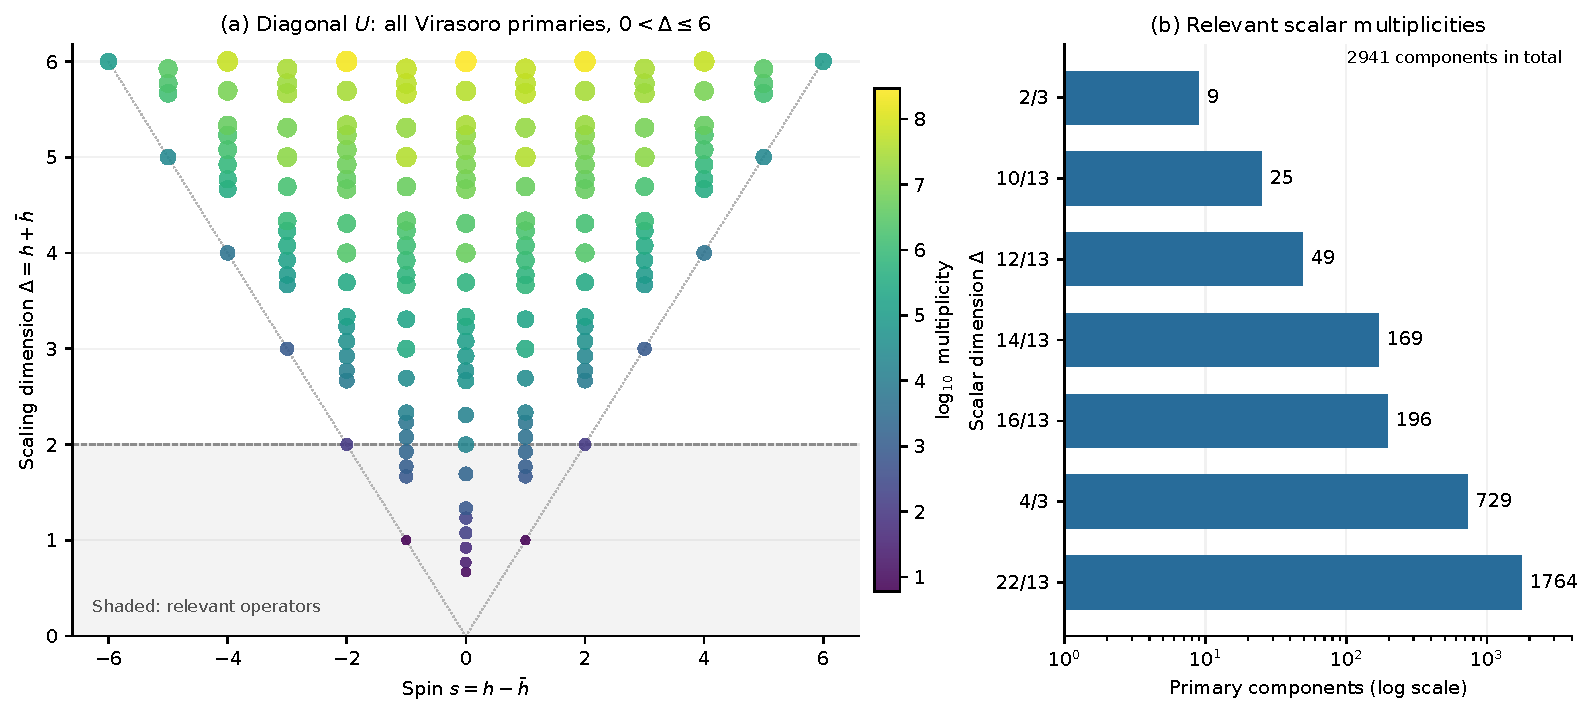
\includegraphics[width=\linewidth]{assets/physics_primary_spectrum.pdf}
\caption{Exact Virasoro-primary spectrum of the diagonal $U$ theory.
Left: all nonidentity $(\Delta,s)$ levels with $0<\Delta\leq6$,
aggregated over the twelve extended sectors; color and marker area
increase with the logarithm of the component multiplicity. The shaded
region has $\Delta<2$. Right: all seven relevant scalar levels,
with their exact multiplicities and a logarithmic count axis.
The identity and Virasoro descendants are excluded.}
\label{fig:physics-primary-spectrum}
\end{figure}
}{}

The complete additional relevant primary levels with nonzero spin
are
\[
\begin{array}{c|c|r}
 \Delta&s&\text{multiplicity for each displayed spin}\\\hline
 1&\pm1&6\\
 5/3&\pm1&720\\
 23/13&\pm1&1120\\
 25/13&\pm1&1995
\end{array}
\]
For example, the second line is $3(243-3)=720$: the three
$c_1$ ground states pair with its $240$ new grade-one Virasoro
primaries.  Including scalars, there are $10623$ nonidentity relevant
Virasoro-primary components.  The ordinary primary gap and the scalar
primary gap are both $2/3$.  There are six currents in each chirality,
generating the affine subalgebra
$\mathfrak{sl}_{2,1}\oplus\mathfrak{sl}_{2,39}$.

At dimension two the scalar-primary multiplicity is
\begin{equation}\label{eq:physics-diagonal-marginal-count}
 80^2+81^2+81^2+6^2=19558.
\end{equation}
The first three terms are the ground spaces of $b,a,c_0$; the final
term comprises the current bilinears $J^A\bar J^B$.  In addition there
are $113$ chiral weight-two primaries in each spin $\pm2$ channel.
Thus dimension two contains $19784$ Virasoro-primary components and
$19798$ states.  The difference consists of the two stress tensors
and twelve current derivatives.  We call dimension-two scalars
\emph{marginal by dimension}; their beta functions and exact
marginality require OPE data not fixed by the character vector.

\subsection{The holomorphic extension and symmetry-preserving perturbations}

For the full $E_8$ theory, the same descendant subtraction gives
$248$ chiral weight-one and $3875$ chiral weight-two Virasoro
primaries.  Consequently its ordinary primary gap is one, its scalar
primary gap is two, and it has no relevant scalar.  The
$\Delta=2$ scalar space has dimension $248^2=61504$; the total
dimension-two state multiplicity is
$2\cdot4124+248^2=69752$.

For the selected canonical extension, the defect construction below
specifies a first chiral $\mathcal H_3$ action inside the full
$\mathcal H_3\boxtimes\mathcal H_3^{\mathrm{op}}$ defect category.
Its invariant Hilbert space is
$U\otimes\overline{H'}$: the first factor acts in its vacuum
representation on $U$ and leaves the antiholomorphic extension
unrestricted.  It therefore has exactly $6\cdot248=1488$ invariant
scalar components at dimension two.  Requiring invariance under
\emph{both independent factors} instead gives
$U\otimes\overline U$ and $6^2=36$ such components.  Each convention
has invariant scalar gap exactly two.  These invariant counts use
the specified canonical-extension defect action, not only the
unflavoured character identity.  Neither count establishes an exactly
marginal family: that requires the corresponding OPE coefficients
and beta functions.

\subsection{Finite-temperature observables with controlled tails}

On a circle of circumference $L$ and velocity $v$, set
$t=\beta v/L$, $b=2\pi t$ and $E=\Delta-2/3$.  Then
\[
 H=\frac{2\pi v}{L}E,\qquad
 P=\frac{2\pi}{L}s,\qquad
 Z(b)=\sum_{\Delta,s}d_{\Delta,s}e^{-b(\Delta-2/3)}.
\]
The ground energy is $-4\pi v/(3L)$.  The exact finite spectral table
already gives a lower bound on $Z$ at every positive temperature.
The following elementary modular estimate also controls the omitted
tail and makes a finite-temperature table quantitatively meaningful.

\begin{proposition}[A tail bound from modular invariance]
\label{prop:physics-modular-tail}
Suppose $Z(b)=Z(4\pi^2/b)$ has nonnegative degeneracies, and that all
states with $\Delta\leq D$ are known, where $D>2/3$.  Write
$Z=L_D+H_D$ for its known and omitted sums, and put
$E_D=D-2/3$.  If $b>2\pi$ and $b'=4\pi^2/b$, then
\begin{equation}\label{eq:physics-thermal-tail}
 0\leq H_D(b)\leq
 \frac{L_D(b)-L_D(b')}{e^{(b-b')E_D}-1}.
\end{equation}
At $b=2\pi$ one has
$0\leq H_D(b)\leq L_D'(b)/E_D$.
For $b<2\pi$ the same bounds apply to $Z(b')=Z(b)$.
\end{proposition}
\begin{proof}
Every omitted energy exceeds $E_D>0$, hence
$H_D(b)\leq rH_D(b')$ with $r=e^{-(b-b')E_D}<1$.
Modular invariance gives
$H_D(b')=H_D(b)+L_D(b)-L_D(b')$; rearranging yields
\eqref{eq:physics-thermal-tail}.  At the fixed point $Z'(2\pi)=0$,
so $L_D'(2\pi)=-H_D'(2\pi)\geq E_DH_D(2\pi)$.
\end{proof}

The real-number rearrangement and the positive-division step at the
fixed point are formalized as
\artifact{modular_heavy_tail_comparison} and
\artifact{selfdual_tail_first_moment_comparison} in
\artifact{lean/HaagerupIzumi/CFT/PhysicsBounds.lean}.
Their hypotheses explicitly include the balance, contraction, and
first-moment inequalities used above. They do not formalize spectral
convergence, the modular functional equation, differentiation of
the trace, or the decimal interval implementation. The guarded
compiler and axiom report is
\artifact{c8_physics_20260927/physics_lean.log}.

To control energy and heat capacity, choose $0<b_0<b$ and bound
$H_D(b_0)$ by the same proposition.  For $k=1,2$,
\begin{equation}\label{eq:physics-moment-tail}
 \sum_{\Delta>D,s}d_{\Delta,s}E^ke^{-bE}
 \leq H_D(b_0)\sup_{E\geq E_D}E^ke^{-(b-b_0)E}.
\end{equation}
The supremum occurs at $E_D$ when $(b-b_0)E_D\geq k$, and otherwise
at $k/(b-b_0)$.  Together with the exact low-energy moments this bounds
$\langle E\rangle$, $C_V=b^2\operatorname{Var}(E)$, and
$S=\log Z+b\langle E\rangle$.  At $t=1$, modular invariance fixes
$\langle E\rangle=0$ exactly.

The supplied thermal tables use $D=24$ and
$t=1/2,3/4,1,3/2,2$, with $b_0=0.9b$ for moment bounds.
The implementation propagates closed decimal intervals with outward
rounding and a rational enclosure of $\pi$; the tables report both
endpoints. The supplied $100$-digit enclosure of $\pi$ is independently
checked by rational alternating sums in Machin's identity
$\pi=16\arctan(1/5)-4\arctan(1/239)$, using $80$ and $25$ terms
with explicit next-term bounds. Their certification is conditional on positivity and
modular invariance of the full CFT, which are mathematical premises
established elsewhere, and not consequences of finite coefficient
agreement.  No unbounded-temperature accuracy claim is made.

For direct comparison the following values are rounded from those
intervals.  Every displayed number has absolute error less than
$10^{-6}$, including both rounding and the omitted-state tail;
the exporter checks this containment before producing the table.
\begin{center}\small
\begin{tabular}{c|c|rrrr}
theory & $t$ & $Z$ & $\langle\Delta-2/3\rangle$ & $C_V$ & $S$\\\hline
$U$ diagonal & $1/2$ & 4367.819471 & 2.653128 & 17.089150 & 16.717068\\
$U$ diagonal & $3/4$ & 303.785760 & 0.983857 & 16.343538 & 10.352640\\
$U$ diagonal & $1$ & 147.219258 & 0.000000 & 19.266968 & 4.991923\\
$U$ diagonal & $3/2$ & 565.179187 & -0.621644 & 3.473060 & 0.478284\\
$U$ diagonal & $2$ & 4367.819471 & -0.663282 & 0.419054 & 0.046971\\
$E_8$ full & $1/2$ & 4356.000000 & 2.659753 & 16.984459 & 16.735170\\
$E_8$ full & $3/4$ & 297.792228 & 0.991916 & 16.622062 & 10.370689\\
$E_8$ full & $1$ & 144.000000 & 0.000000 & 19.157072 & 4.969813\\
$E_8$ full & $3/2$ & 557.169604 & -0.627321 & 3.435582 & 0.410512\\
$E_8$ full & $2$ & 4356.000000 & -0.664938 & 0.272738 & 0.023449\\
\end{tabular}

\end{center}

\IfFileExists{assets/physics_thermal_comparison.pdf}{%
\begin{figure}[htbp]
\centering
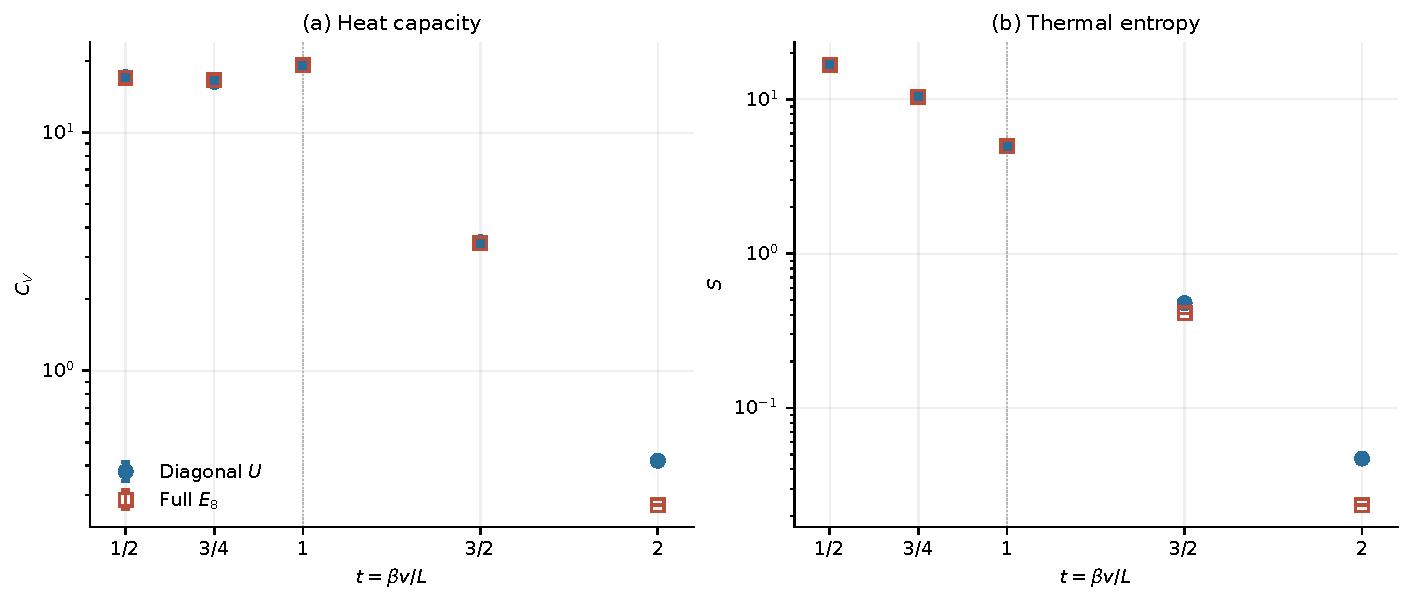
\includegraphics[width=\linewidth]{assets/physics_thermal_comparison.pdf}
\caption{Heat capacity and thermal entropy of the two full theories at
the five computed temperatures $t=\beta v/L$. Both vertical axes are
logarithmic. No interpolation is drawn. Error bars come from the
conditional certified intervals using all states through $\Delta=24$
and the modular/moment tail bounds; they are smaller than the markers.
The dotted line marks the modular fixed point $t=1$.}
\label{fig:physics-thermal}
\end{figure}
}{}

In the thermodynamic limit both theories have
\[
 f(T)-f(0)=-\frac{4\pi}{3v}T^2,
 \qquad s(T)=\frac{C_V(T)}L=\frac{8\pi}{3v}T.
\]
Their universal single-interval ground-state entanglement coefficient
is $8/3$ in front of $\log(\ell/\epsilon)$, and the R\'enyi coefficient
is $\frac43(1+n^{-1})$.  These central-charge observables do not
distinguish the diagonal theory from its holomorphic extension;
the low-energy spectrum and defect-resolved observables do.

\subsection{Dataset, reproducibility, and limits}

The standalone standard-library producer is
\artifact{c8_physics_20260927/spectrum.py}.  Its default run computes
24 grades of all twelve characters, including Virasoro-primary
multiplicities, and complete spectra through $\Delta=24$ for both
full theories.  The output directory contains
\artifact{characters.json}, \artifact{characters.tsv},
\artifact{fundamental_matrix.json},
\artifact{diagonal_sector_spectrum.tsv},
\artifact{diagonal_spectrum.tsv}, \artifact{e8_spectrum.tsv},
\artifact{scalars.tsv}, \artifact{low_spectrum.json},
\artifact{thermal.json}, and \artifact{thermal.tsv}.
The run summary records coefficient controls, nonnegative integrality,
descendant reconstruction, spin reflection, the $E_8$ product check,
and source/output hashes.  Paths in this paragraph are relative to
\artifact{c8_physics_20260927/data/}, except the explicitly named
producer.

For a replay into a fresh directory, run serially from the repository
root (ordinary Python, without optimization):
\begin{verbatim}
python hi_cft_safe_run.py --limit-mib 512 -- \
  python c8_physics_20260927/spectrum.py --order 24 --delta-cut 24 \
  --outdir /tmp/c8-physics-spectrum-replay
\end{verbatim}
Existing output files are not overwritten. The address cap in this
command is lower than the permanent machine limit; the launcher also
retains its host-memory reserve, process-group watchdog, and two-CPU
limit.

The spectrum exporter determines unflavoured graded dimensions and
the stated thermal observables.  It does not compute normalized
three-point coefficients, crossing matrices of conformal blocks,
defect eigenvectors, or branching characters with Cartan fugacities.
The separate defect and correlator datasets below provide further
information of those kinds in their stated scopes.  In particular an
exclusion plot that resolves Haagerup charges uses the specified
defect-sector decomposition; ordinary unflavoured gaps alone do not
supply its inputs.

\section{Exact correlators and channel data}
\label{sec:physics-correlators}

The vacuum algebra gives several explicit interacting chiral correlators,
in addition to current and stress-tensor Ward identities.  We give two
four-point functions of the weight-two generator, two spin-three four-point
functions, and selected intertwiner blocks for the lightest nonvacuum
module.  All normalizations below are fixed.  The last family consists of
chiral blocks obtained from the containing lattice theory; it does not
specify the diagonal $U$ theory's nonvacuum bulk four-point function.

\subsection{Conventions and Ward identities}

Write $T$ for the total stress tensor, with
\begin{equation}
 T(z)T(0)\sim \frac{4}{z^4}+\frac{2T(0)}{z^2}
                   +\frac{\partial T(0)}{z}.
\end{equation}
The two commuting affine $\mathfrak{sl}_2$ algebras have levels
$k_L=1$ and $k_R=39$.  We use Cartan currents with
$H_L(z)H_L(0)\sim2z^{-2}$ and
$H_R(z)H_R(0)\sim78z^{-2}$; their mixed two-point function vanishes.
More generally, for invariant form $\kappa$ normalized by
$\kappa(H,H)=2$, the currents obey
\begin{equation}
 J^a(z)J^b(0)\sim\frac{k\kappa^{ab}}{z^2}
               +\frac{f^{ab}{}_cJ^c(0)}{z}.
\end{equation}
This fixes every vacuum current correlator recursively.  For example,
with $f^{abc}=f^{ab}{}_d\kappa^{dc}$,
$\langle J^a(z_1)J^b(z_2)J^c(z_3)\rangle
=k f^{abc}/(z_{12}z_{13}z_{23})$.

Let $\widehat u=u/\sqrt{12}$ and let $\widehat u^\dagger$ denote its
chiral adjoint in the transported positive lattice form.  The symbol
$\dagger$ does not introduce an antiholomorphic field.  This primary has
weight two, Cartan charges $(q_L,q_R)=(1,13)$, and
\begin{align}
 \langle\widehat u(z)\widehat u^\dagger(0)\rangle&=z^{-4},\\
 \langle H_a(z_1)\widehat u(z_2)\widehat u^\dagger(z_3)\rangle
  &=\frac{q_a}{z_{12}z_{13}z_{23}^{3}},\\
 \langle T(z_1)\widehat u(z_2)\widehat u^\dagger(z_3)\rangle
  &=\frac{2}{z_{12}^{2}z_{13}^{2}z_{23}^{2}}.
\end{align}
Consequently the squared couplings to the unit Cartan currents are
$1/2$ and $13/6$.  A useful mixed four-point function is
\begin{equation}
 \begin{aligned}
 \langle H_a(z_1)H_b(z_2)\widehat u(z_3)
                  \widehat u^\dagger(z_4)\rangle
 ={}&\frac{1}{z_{34}^{4}}\left[
 \frac{K_{ab}}{z_{12}^{2}}+
 q_aq_b\left(\frac1{z_{13}}-\frac1{z_{14}}\right)
       \left(\frac1{z_{23}}-\frac1{z_{24}}\right)\right].
 \end{aligned}
\end{equation}
Here $K=\operatorname{diag}(2,78)$.
The unit stress tensor is $\widehat T=T/2$; both
$C_{\widehat T\widehat u\widehat u^\dagger}$ and
$C_{\widehat T\widehat T\widehat T}$ equal one in these conventions.
Writing $y=1-x$, the normalized four-point functions of any unit
Cartan current $\widehat H$ and of $\widehat T$ are
\begin{align}
 \langle\widehat H(\infty)\widehat H(1)
                 \widehat H(x)\widehat H(0)\rangle
 &=1+x^{-2}+y^{-2},\\
 \langle\widehat T(\infty)\widehat T(1)
                 \widehat T(x)\widehat T(0)\rangle
 &=1+x^{-4}+y^{-4}+x^{-2}+y^{-2}+x^{-1}+y^{-1}.
\end{align}
The first follows from Heisenberg Wick contractions, the second from
the Virasoro Ward identity at central charge eight.

\subsection{A three-exponential four-point function}

In simple-root coordinates of $E_6\oplus A_2$, put
\begin{align}
 a_1&=(0,0,0,0,0,-1,1,1),\\
 a_2&=(0,0,0,1,1,-1,0,0),\\
 a_3&=(1,1,0,0,0,-1,0,0),\\
 u&=e^{a_1}+\frac{\sqrt{13}+3\sqrt{-3}}{20}e^{a_2}
             +\frac{\sqrt{13}-3\sqrt{-3}}{20}e^{a_3}.
\end{align}
The simple-root Gram matrix has diagonal entries two and entries minus
one along the edges $(0,1),(1,2),(2,3),(3,4),(2,5),(6,7)$, with indices
starting at zero.  Thus $(a_i,a_i)=4$ and $(a_i,a_j)=2$ for $i\ne j$.
In the torus gauge $(5,8,9,8,5,1,2,2)$, the three exponential squared
norms are $4,40,40$.  Their coefficients therefore contribute $4,4,4$
to $\|u\|^2=12$.  In particular this calculation uses the transported
positive form, rather than treating the three displayed coefficients as
coordinates in an orthonormal basis.

The lattice Gaussian formula in a specified cocycle gauge is
\begin{equation}
 \left\langle\prod_{j=1}^{n}e^{b_j}(z_j)\right\rangle
 =\delta_{\sum_j b_j,0}\,
   \varepsilon(b_1,\ldots,b_n)
   \prod_{i<j}(z_i-z_j)^{(b_i,b_j)}.
\end{equation}
Here the integer-lattice cocycle is
\begin{equation}
 \varepsilon(a,b)=(-1)^{\sum_i a_i b_i+
                  \sum_{i>j}a_i b_jG_{ij}},
\end{equation}
and the multivariable factor is its iterated product.  These formulas
also give a short independent derivation: expand each of the four
fields, discard nonzero total charge, and multiply their six pairwise
Gaussian factors.  Of the $3^4=81$ terms, fifteen survive.  All fifteen
have coefficient $1/9$ after inserting the adjoint gauge and normalizing
the four external fields.

Set the insertion points to $(\infty,1,x,0)$, with
$\phi(\infty)=\lim_{R\to\infty}R^{2h}\phi(R)$.  The two useful
reflection-positive channels are
\begin{align}
 G_0(x)&=\langle\widehat u^\dagger(\infty)\widehat u(1)
                 \widehat u^\dagger(x)\widehat u(0)\rangle
       =\boxed{\frac{3-4x+4x^2}{3x^4(1-x)^4}},
       \label{eq:physics-u-neutral}\\
 G_+(x)&=\langle\widehat u^\dagger(\infty)\widehat u^\dagger(1)
                 \widehat u(x)\widehat u(0)\rangle
       =\boxed{\frac{x^2(4-4x+3x^2)}{3(1-x)^4}}.
       \label{eq:physics-u-charged}
\end{align}
For example, the fifteen neutral contributions to the first formula
sum to
\begin{equation}
 \frac{1}{3x^4(1-x)^4}
 +\frac{2}{3x^2(1-x)^4}
 +\frac{2}{3x^4(1-x)^2}.
\end{equation}
The three inequivalent orderings follow from
$G_0(1-x)=G_0(x)$,
$G_+(x)=x^{-4}G_0(1/x)$, and $G_+(1-x)$; their adjoint orderings agree.
These are exact rational identities, not truncated series fits.

To display positive channel data, expand in global conformal blocks:
\begin{equation}
 x^{2h_{\rm ext}}G(x)=A_0+
       \sum_{n\ge1}A_n x^n\,{}_2F_1(n,n;2n;x).
 \label{eq:physics-global-block-convention}
\end{equation}
For the two channels above, $A_n$ is the sum of squared couplings to
orthonormal global quasiprimaries of weight $n$ in the appropriate charge
sector.  This statement uses the positive radial pairing.  It does not
identify $A_n$ with a single primary coupling or a Virasoro block
coefficient.  The first neutral coefficients are
\begin{equation}
 (A_0,A_1,A_2,A_3,A_4)
 =\left(1,\frac83,\frac{14}3,\frac{58}9,\frac{107}{15}\right).
\end{equation}
The value $A_1=1/2+13/6$ reproduces the two Cartan-current exchanges.
At weight two the total stress tensor contributes one, leaving
$11/3$ as the squared-coupling sum to ambient Virasoro primaries.
In the equal-charge channel the first nonzero coefficient is
$A_6=4/3$, followed by $A_8=19/13$; odd weights vanish.  Indeed,
the leading state $\widehat u_{(-3)}\widehat u$ is supported on the
three momenta $a_i+a_j$ with $i<j$, each of norm squared twelve.
It is a weight-six Virasoro primary of squared norm $4/3$.
The normalized leading OPE coefficient can therefore be chosen
$2/\sqrt3$.  In particular the equal-charge OPE vanishes through
orders $x^0$ and $x^1$ and starts at $x^2$.

The four orthogonal commuting stress tensors give additional resolved
weight-two data.  If $T_i$ has central charge $c_i$ and $u$ has
$T_i$-weight $h_i$, then
$C_{\widehat T_i\widehat u\widehat u^\dagger}^2=2h_i^2/c_i$.
Here the entries are
\begin{center}
\begin{tabular}{c|c|c|c}
stress & $c_i$ & $h_i$ & squared unit-field coupling\\\hline
$T_L$ & $1$ & $1/4$ & $1/8$\\
$T_R$ & $117/41$ & $195/164$ & $325/328$\\
$e$ & $2400/1271$ & $180/1271$ & $27/1271$\\
$f$ & $70/31$ & $13/31$ & $169/1085$
\end{tabular}
\end{center}
Their charges and weights sum to eight and two, respectively.

\subsection{Potts and parafermion spin-three four-point functions}

The embedded Potts and parafermion algebras contain canonical spin-three generators with
parameters
\begin{equation}
 (c,\lambda)=\left(\frac45,\frac4{13}\right)
 \quad\hbox{and}\quad
 (c,\lambda)=\left(\frac85,\frac{14}{473}\right).
\end{equation}
These are the Potts and level-thirteen parafermion cases, in the
normalization of the universal $\mathcal W(c,\lambda)$ algebra
\cite{Linshaw,DLY}.  Denote either spin-three field by $a$, its intrinsic
stress tensor by $T_c$, and put
\begin{equation}
 N=\frac c3,\qquad b=a_{(1)}a,\qquad
 A=31-16\lambda(c+2),\qquad B=NA.
\end{equation}
The exact checked singular self-OPE is
\begin{align}
 a(z)a(0)\sim{}&\frac{N}{z^6}+\frac{2T_c}{z^4}
 +\frac{\partial T_c}{z^3}+\frac{b}{z^2}
 +\frac{\frac12\partial b-\frac1{12}\partial^3T_c}{z},
 \label{eq:physics-spin3-ope}\\
 a_{(3)}b={}&Aa,\qquad \|b\|^2=B.
\end{align}
The positive normalization is chosen so that $a$ has two-point
coefficient $N$; write $\widehat a=a/\sqrt N$.  The exact values of
$(A,B)$ are $(1119/65,1492/325)$ for Potts and
$(69283/2365,554264/35475)$ for the parafermion generator.

Meromorphy, the OPE and crossing determine the complete correlator:
\begin{align}
 N^2\langle\widehat a(\infty)\widehat a(1)
                 \widehat a(x)\widehat a(0)\rangle
 ={}&N^2\bigl[1+x^{-6}+(1-x)^{-6}\bigr]\nonumber\\
 &+2c\bigl[x^{-4}+(1-x)^{-4}
             +x^{-3}+(1-x)^{-3}\bigr]\nonumber\\
 &+B\bigl[x^{-2}+(1-x)^{-2}\bigr]
 +(2B-2c)\bigl[x^{-1}+(1-x)^{-1}\bigr].
 \label{eq:physics-spin3-fourpoint}
\end{align}
For completeness, the principal part at zero follows by pairing the
five terms of \eqref{eq:physics-spin3-ope} with the outer two fields.
The Ward identity gives
$\langle a(\infty)a(1)T_c(0)\rangle=3N$; its first derivative is
$6N$, and its third derivative is $72N$.  Likewise
$\langle a(\infty)a(1)b(0)\rangle=B$, whose first derivative is
$4B$.  These give residues $N^2,2c,2c,B,2B-2c$ at pole orders
$6,4,3,2,1$.  Interchange of the equal fields fixes the principal part
at one.  The identity channel at infinity fixes the constant $N^2$.
The difference between the displayed function and the correlator is
therefore a holomorphic function on the sphere vanishing at infinity.
Both crossing generators $x\mapsto1-x$ and $x\mapsto1/x$ can also be
verified directly in the displayed expression.

The self-cubic coefficient $C_{\widehat a\widehat a\widehat a}$
vanishes.  The squared coupling to the unit intrinsic stress tensor is
$18/c$.  To isolate the new weight-four channel from Virasoro
descendants, put
\begin{equation}
 \Lambda=:T_cT_c:-\frac3{10}\partial^2T_c,
 \qquad \|\Lambda\|^2=\frac{c(5c+22)}{10},
 \qquad W_4^{\rm prim}
 =b-\frac{32}{5c+22}\Lambda-\frac3{10}\partial^2T_c.
\end{equation}
The squared $\widehat a\widehat a\Lambda/\|\Lambda\|$ coupling
is $4608/[5c(5c+22)]$.  Subtracting this contribution from the global
weight-four coefficient gives
\begin{equation}
 \gamma_4^2
 =\frac{48(c+2)\{8-\lambda(5c+22)\}}{c(5c+22)}
 =\begin{cases}
 0,&\text{Potts},\\
 60552/2365,&\text{level-thirteen parafermion}.
 \end{cases}
\end{equation}
Thus the Potts extra weight-four primary is null, whereas the
parafermion channel has a strictly positive extra coupling.  This
separation refers to the intrinsic Virasoro algebra of central charge
$c$, not to the total central-charge-eight Virasoro algebra.  The
corresponding total global weight-four coefficients are $576/13$ and
$21192/473$.  Equation \eqref{eq:physics-spin3-fourpoint} supplies all
higher global coefficients without a new high-weight mode calculation.

\subsection{Selected blocks for the lightest module}

The two $B$-lattice sectors $(0,+1)$ and $(0,-1)$ both restrict to the
simple $U$-module $c_1$ of lowest weight $1/3$ and top dimension three.
In the $A_2$ simple-root basis its three fundamental weights are
\begin{equation}
 \beta_0=(2/3,1/3),\quad
 \beta_1=(-1/3,1/3),\quad
 \beta_2=(-1/3,-2/3),\qquad
 (\beta_i,\beta_j)=\delta_{ij}-\frac13.
\end{equation}
Their $H_R$ charges are $q=(2,0,-2)$; their $H_L$ charges vanish.
Choose paired lattice intertwiners with unit leading vacuum coefficient.
On the branch $0<x<1$ with positive real powers, the nine selected
four-point blocks are
\begin{equation}
 \mathcal F_{ij}(x)
 =\langle V_{-\beta_i}(\infty)V_{\beta_i}(1)
           V_{-\beta_j}(x)V_{\beta_j}(0)\rangle
 =\boxed{x^{-2/3}(1-x)^{-(\beta_i,\beta_j)}}.
 \label{eq:physics-lightest-block}
\end{equation}
Thus the diagonal entries are $[x(1-x)]^{-2/3}$ and the off-diagonal
entries are $x^{-2/3}(1-x)^{1/3}$.  Analytic continuation requires a
specified path; the fractional powers must not be replaced by a
single-valued rational function.

In the $x\to0$ channel these blocks factor through the $B$ vacuum
sector, whose restriction is $U\oplus X$, with $X$ the module denoted
$b$ in the modular table.  The first coefficient of the reduced block
is $(\beta_i,\beta_j)$.  The decomposition of the intermediate
weight-one Heisenberg vector gives the explicit split
\begin{equation}
 (\beta_i,\beta_j)
 =\underbrace{\frac{q_iq_j}{78}}_{U\text{ current exchange}}
 +\underbrace{\left(\beta_i,\beta_j\right)
                    -\frac{q_iq_j}{78}}_{X\text{ top exchange}}.
\end{equation}
For $i=j=0$ these two positive coefficients are $2/39$ and $8/13$.
The three-by-three $X$ Gram matrix has eigenvalues $0,1,35/39$,
providing a direct positive-channel check.  Off-diagonal entries need
not be positive: they are overlaps, rather than squared norms.
The six ordered triples with three distinct weights have nonzero
three-point functions proportional to
$(z_{12}z_{13}z_{23})^{-1/3}$, with coefficient of absolute square one
in this normalization.  Their phases depend on the lattice-intertwiner
cocycle and chosen bases.  Two distinct positive weights add to the
negative of the remaining weight and hence exhibit a $c_1$ channel.

Restriction of a lattice intertwiner gives a genuine $U$ intertwiner,
so these are nonvacuum chiral data, beyond Ward identities.  Their
particular linear combinations and normalizations remember the
extension $U\subset B$.  They neither form a complete basis of all
$U$ channels nor determine the diagonal theory's local bulk correlator
$\langle\Phi\Phi\Phi\Phi\rangle$ for its lightest scalar.
That quantity additionally requires channel and multiplicity bases,
the full relevant intertwining operators and the left-right sewing
coefficients.  In particular, multiplying one selected block by its
complex conjugate has not been justified as that bulk correlator.

\subsection{Reproducible data and verification scope}

The bounded standard-library script
\artifact{c8_physics_20260927/correlators.py} exports
\artifact{c8_physics_20260927/correlators.json}, together with the
tables \artifact{c8_physics_20260927/correlators.terms.tsv},
\artifact{c8_physics_20260927/correlators.global_blocks.tsv}, and
\artifact{c8_physics_20260927/correlators.samples.tsv}.
The first table retains all $486$ assignments across the six charge
orderings, including vanishing terms, their cocycle signs and exact
coefficients in $\mathbb Q(\sqrt{13},\sqrt{-3})$.
The second gives the exact global-block decomposition of the two
$u$ channels, both spin-three correlators and the two Ward correlators through the recorded
cutoff, with default weight $32$; the third gives exact values at five
rational cross-ratios.  Polynomial crossing identities, reconstruction
of the truncated series, positivity in the specified channels and the
lightest-module Gram decomposition are checked exactly.

The script checks the three-exponential input against
\artifact{hi_cft_20260923_c8_exact_fields.json}.  The spin-three
parameters and norms are read from
\artifact{hi_cft_20260923_proof_pf13_ope.json}; their singular OPE
provenance is
\artifact{hi_cft_20260923_proof_pf13_upper_poles.py} and its saved
report.  Source hashes are included.  The export does not import the
lattice mode engine or repeat its higher-grade computations.  Its
finite positivity tests provide reproducible consistency checks;
all-order positivity follows here from the positive VOA realization,
rather than from extrapolating those tests.  The separately exported
low-weight coupling tensor resolves many of the summed weight-two
channels above into individual normalized primary couplings.

\section{A complete weight-two chiral three-point dataset}
\label{sec:physics-couplings}

The coefficient $120$ of the vacuum character is small enough to
resolve its first interacting primary space completely. Its $113$
Virasoro primaries comprise the $96$ fields in the eight charged
current multiplets of the construction, together with $17$ fields
obtained from the currents and stress tensors. Here ``charged'' refers
to a nontrivial current multiplet; it does not exclude zero-weight
components within that multiplet.

\subsection{Actual fields and normalization}

Label the eight original highest fields by $v_{m,0,0}$,
$m=0,\ldots,7$, in the order
\[
 (n_m,r_m)=(1,5),(1,9),(1,9),(1,13),
            (2,2),(2,6),(2,8),(2,14).
\]
These are representation dimensions for the two current algebras.
The two $(1,9)$ copies are distinct and have different coset-stress
eigenvalues. In the last multiplet the highest field is the defining
field $u$, with the normalization inherited from its saved lattice
vector. Define all components by
\begin{equation}\label{eq:physics-primary-basis}
 v_{m,p,q}=(F_L)_0^p(F_R)_0^qv_{m,0,0},
 \quad 0\leq p<n_m,\quad0\leq q<r_m.
\end{equation}
No factorials divide the lowering powers. The Cartan charges are
$(n_m-1-2p,r_m-1-2q)$.

The remaining highest fields are
\[
 v_{8,0,0}=(E_R)_{-1}E_R,\qquad
 v_{9,0,0}=(E_L)_{-1}E_R,
\]
of current types $(1,5)$ and $(3,3)$, and three current singlets.
To specify the latter, use the four mutually commuting stress tensors
\[
 (T_L,T_R,T_e,T_f),\qquad
 (c_L^{\rm aff},c_R^{\rm aff},c_e,c_f)
 =\left(1,\frac{117}{41},\frac{2400}{1271},\frac{70}{31}\right).
\]
In the next formula abbreviate the first two central charges by
$c_l,c_r$, to distinguish them from the spacetime charges $c_L=c_R=8$.
The singlets are
\begin{align}
 v_{10,0,0}&=c_rT_L-c_lT_R,\\
 v_{11,0,0}&=c_e(T_L+T_R)-(c_l+c_r)T_e,\\
 v_{12,0,0}&=c_f(T_L+T_R+T_e)-(c_l+c_r+c_e)T_f.
 \label{eq:physics-stress-primaries}
\end{align}
Because $\langle T_i,T_j\rangle=\delta_{ij}c_i/2$, these three
vectors are mutually orthogonal and orthogonal to the total stress
tensor. A combination $\sum a_iT_i$ is a total-Virasoro primary
exactly when $\sum a_ic_i=0$, proving their primarity directly.

The right spin-two multiplet is the traceless symmetric current
product. The cross-current multiplet is primary because the two
current factors commute. At level one the left spin-two current
product is null, so there is no additional $(5,1)$ multiplet.
Together these add $5+9+3=17$ fields. The exact calculation checks
the Virasoro-primary conditions, all possible off-diagonal Gram
entries within equal Cartan weights, and positive norms for all
$113$ vectors. Distinct Cartan weights are orthogonal by the compact
real form. Their independence and the character count
$120-6-1=113$ prove completeness: the subtractions remove six current
derivatives and the total stress tensor.

Put $N_i=\langle v_i,v_i\rangle_g$ and
$\widehat v_i=v_i/\sqrt{N_i}$, choosing the positive square root.
The exported coefficients use the antilinear first-slot Hermitian
pairing and the transported lattice PCT of \eqref{eq:pct}:
\begin{equation}\label{eq:physics-primary-three-point}
 C_{ij}^{\ k}
 =\langle\widehat v_k,(\widehat v_i)_1\widehat v_j\rangle_g
 =\frac{\langle v_k,(v_i)_1v_j\rangle_g}
 {\sqrt{N_iN_jN_k}}.
\end{equation}
Equivalently this is the three-point coefficient with the conjugate
of $\widehat v_k$ at infinity. The singular OPE contains
$z^{-2}C_{ij}^{\ k}\widehat v_k(0)$, in addition to current,
stress-tensor and descendant contributions. The unnormalized
numerator and norm product lie in
$\mathbb Q(\sqrt{13},\sqrt{-3})$; the positive square-root
normalization is left explicit. Thus the table retains the complex
phase, not only $|C|^2$.

\subsection{From directly computed seeds to the full tensor}

Let $P$ be orthogonal projection onto this primary space and write
$P((v_i)_1v_j)=\sum_k p_{ij}^{\ k}v_k$. Since current zero modes
commute with the total Virasoro algebra, this projection is equivariant.
For either lowering operator $F$ the derivation identity gives
\begin{equation}\label{eq:physics-Ward-completion}
 P((Fv_i)_1v_j)=F\,P((v_i)_1v_j)-P((v_i)_1Fv_j).
\end{equation}
Starting with $i$ highest in each of the thirteen multiplets determines
the entire tensor recursively. In the raw basis \eqref{eq:physics-primary-basis},
$F$ simply advances one lowering exponent; its raising partner acts
by $E v_p=p(n-p)v_{p-1}$. Equation~\eqref{eq:physics-Ward-completion}
therefore uses only exact additions and multiplications of known
coefficients. Orthogonal projection is essential here: we do not
discard descendants before justifying equivariance.

The direct seed calculation evaluates $1137$ actual lattice mode
products and $3512$ charge-compatible projections, of which $1639$
are nonzero. The completed tensor has
\[
 113^3=1442897\quad\hbox{ordered entries},\qquad
 18365\quad\hbox{nonzero entries}.
\]
All omitted entries in the sparse table are exactly zero within this
complete weight-two primary tensor. Every raising and lowering Ward
identity is checked, including at the tops and bottoms of multiplets:
there are $51076$ pairwise checks. Primary skew-symmetry gives a
further $12769$ checks, and $33$ additional direct lattice products
test components outside the initial seed slice. These checks verify
the specified finite tensor; they are not a test of arbitrary-weight
associativity or full-CFT sewing.

A cross-check connects this tensor to an independent four-point
calculation. The weight $(-1,-13)$ component is unique, so
$\widehat v_{7,1,13}$ equals $\widehat u^\dagger$ up to a phase.
Summing its nine nonzero primary projections gives exactly
\[
 \sum_{k=1}^{113}|C_{\widehat u,\widehat u^\dagger}^{\ k}|^2
 =\frac{11}{3}.
\]
Adding the total-stress contribution one reproduces the global
weight-two coefficient $14/3$ in the Gaussian four-point function
\eqref{eq:physics-u-neutral}. The three stress-difference contributions
separately agree with their Ward values. The small standalone checker
\artifact{check_physics_crosslinks.py} verifies these sums without
importing the lattice mode engine.

Several entries are short enough to check without navigating a large
file. The indices below are the explicit $(m,p,q)$ labels above.
\begin{center}
\begin{tabular}{ccc|r}
\toprule
$i$&$j$&$k$&$|C_{ij}^{\ k}|^2$\\
\midrule
$(0,0,0)$&$(0,0,2)$&$(0,0,0)$&$4356/8645$\\
$(1,0,0)$&$(1,0,6)$&$(0,0,0)$&$39605/717288$\\
$(7,0,0)$&$(7,1,13)$&$(10,0,0)$&$13/316$\\
$(8,0,0)$&$(8,0,3)$&$(8,0,1)$&$1225/741$\\
$(9,0,0)$&$(9,2,0)$&$(8,0,0)$&$76/39$\\
$(10,0,0)$&$(10,0,0)$&$(10,0,0)$&$23104/9243$\\
$(12,0,0)$&$(12,0,0)$&$(12,0,0)$&$2916/3115$\\
\bottomrule
\end{tabular}
\end{center}
For example, for $A=c_rT_L-c_lT_R$ one has
\[
 \langle A,A\rangle=\frac{c_lc_r(c_l+c_r)}2,\qquad
 |C_{AAA}|^2=\frac{8(c_r-c_l)^2}{c_lc_r(c_l+c_r)}
 =\frac{23104}{9243}.
\]
This follows just from the two commuting stress OPEs and provides a
human-sized independent normalization check on the lattice table.

The principal files are
\artifact{c8_physics_20260927/full_weight_two/low_weight_basis.json},
which stores every actual lattice vector and norm;
\artifact{low_weight_products.jsonl}, which stores each seed product;
and \artifact{complete_primary_couplings.tsv}, which stores every
nonzero normalized coefficient by its exact numerator and norm product.
The accompanying JSON report documents the recurrence checks and
source hashes. The earlier $96$-field slice remains available as an
intermediate audit, but the $113$-field table is the complete release.

These are chiral vacuum-module observables of $U$, hence also
observables of its selected extension. They give local spinning fields
in either bulk theory. Factorized products of these fields give
additional full-CFT vacuum-sector correlators. They do not supply the
three-point constants of generic nonvacuum diagonal-sector primaries.

\section{Modular data, topological defects, and conformal boundaries}
\label{sec:physics-defects}

We use the positive spherical structure and the Evans--Gannon ordering
\[
 (0,b,a,c_0,c_1,c_2,d_1,d_2,d_3,d_4,d_5,d_6).
\]
The translation to the labels used in the Haagerup bootstrap literature is
\[
 (1,\pi_1,\pi_2,\sigma_1,\sigma_2,\sigma_3,
   \mu_5,\mu_2,\mu_1,\mu_3,\mu_6,\mu_4).
\]
The final permutation is fixed by the distinct thirteenth-root twists
in \cite[arXiv version~2, Eq.~(30)]{AHKZ}; retaining the same numerical subscripts for
the $d$ and $\mu$ labels would be incorrect.
In particular, $a$ is a simple object of the center, whereas $\alpha$
below denotes the invertible generator of the six-object Haagerup
category. These two objects have different dimensions and different roles.

Put $r=\sqrt{13}$, $d=(3+r)/2$, $s=2+3d$, and
\[
 A=\frac16-\frac1{2r},\qquad B=\frac16+\frac1{2r},\qquad
 u=\frac13,\qquad v=\frac1r.
\]
In blocks of sizes $1,1,4,6$, the complete normalized matrix is
\begin{equation}
 S=\begin{pmatrix}
 A&B&u\mathbf1_4^{\mathsf t}&v\mathbf1_6^{\mathsf t}\\
 B&A&u\mathbf1_4^{\mathsf t}&-v\mathbf1_6^{\mathsf t}\\
 u\mathbf1_4&u\mathbf1_4&C&0\\
 v\mathbf1_6&-v\mathbf1_6&0&D
 \end{pmatrix},
 \qquad
 C=\frac13\begin{pmatrix}
 2&-1&-1&-1\\-1&2&-1&-1\\-1&-1&-1&2\\-1&-1&2&-1
 \end{pmatrix},
 \label{eq:physics-S}
\end{equation}
where
\begin{equation}
 D_{ij}=-\frac2{\sqrt{13}}\cos\frac{2\pi ij}{13},
 \qquad 1\leq i,j\leq6.
 \label{eq:physics-Sd}
\end{equation}
The topological twist matrix and the character matrix are distinct:
\begin{align}
 \Theta&=\operatorname{diag}\left(
 1,1,1,1,e^{2\pi i/3},e^{4\pi i/3},
 e^{2\pi i6/13},e^{2\pi i11/13},e^{2\pi i2/13},
 e^{2\pi i5/13},e^{2\pi i7/13},e^{2\pi i8/13}\right),\\
 T_{\rm ch}&=e^{-2\pi i/3}\Theta.
 \label{eq:physics-T}
\end{align}
Thus the $d_j$ twist is $e^{2\pi i6j^2/13}$. The conformal weight of
$d_3$ is $15/13$, although its twist exponent is $2/13$.
These are the standard positive Haagerup modular data
\cite{EG}; no numerical eigenvector choice enters these formulas.

The categorical dimensions and total quantum dimension are
\begin{equation}
 (\operatorname{qdim}M_i)_i=(1,d^2,s,s,s,s,3d,3d,3d,3d,3d,3d),
 \qquad \mathcal D=\frac1{S_{00}}=3s.
 \label{eq:physics-qdim}
\end{equation}
Here $\mathcal D^2$, rather than $\mathcal D$, is the global dimension
of $\operatorname{Rep}(U)$. Every simple object is self-dual because
$S^2=1$. The six-object Haagerup category has global dimension
$3+3d^2=3s=\mathcal D$.

\begin{figure}[tbp]
 \centering
 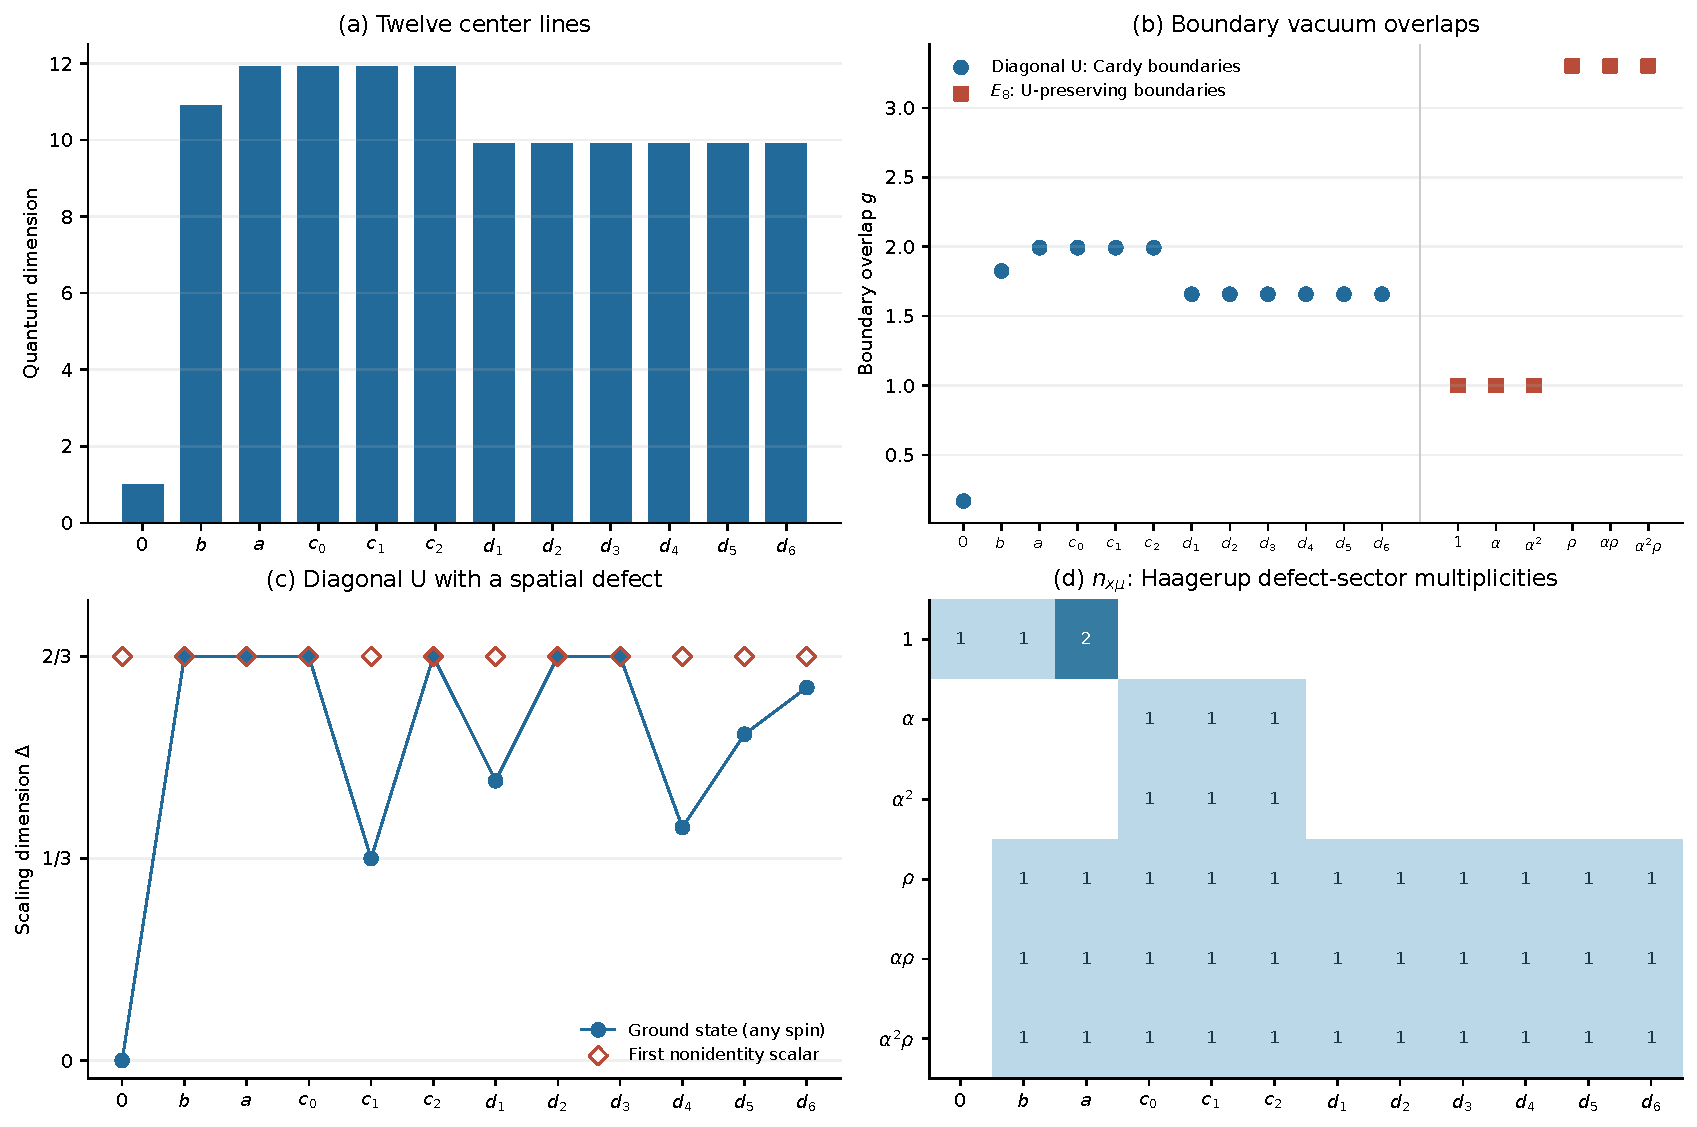
\includegraphics[width=\textwidth]{assets/defect_observables.pdf}
 \caption{Exact modular and defect observables, displayed using the
 positive embedding of the exported algebraic data. The ground-state
 gap in a twisted space and its scalar gap are distinct; the latter
 is $2/3$ for all twelve diagonal-theory lines. The final panel records
 the integer forgetful multiplicity matrix for the selected extension.}
 \label{fig:physics-defects}
\end{figure}

\subsection{Exact fusion and diagonal-theory defect spectra}

Consider first the diagonal full CFT
\begin{equation}
 \mathcal H_U=\bigoplus_i M_i\otimes\overline{M_i},
 \qquad Z_U(\tau,\bar\tau)=\sum_i|\chi_i(\tau)|^2.
\end{equation}
Its twelve chiral-algebra-preserving Verlinde lines form the fusion
category underlying $\operatorname{Rep}(U)=Z(\mathcal H_3)$.
Their multiplication and their action on bulk sectors are
\begin{equation}
 N_{ab}^{\phantom{ab}c}
   =\sum_i\frac{S_{ai}S_{bi}S_{ci}}{S_{0i}},
 \qquad
 \widehat L_a\big|_{M_i\otimes\overline{M_i}}
   =\lambda_a(i)\,\mathrm{id},
 \qquad \lambda_a(i)=\frac{S_{ai}}{S_{0i}}.
 \label{eq:physics-Verlinde}
\end{equation}
Complex conjugation is absent from the displayed Verlinde sum because
$S$ is real. In particular $\lambda_a(0)=\operatorname{qdim}(M_a)$.
The line insertion and its modular transform give
\begin{align}
 Z_U^{[a]}(\tau,\bar\tau)
   &=\sum_i\lambda_a(i)|\chi_i(\tau)|^2,\\
 Z_{U,[a]}(\tau,\bar\tau)
   &=\sum_{i,j}N_{ai}^{\phantom{ai}j}
           \chi_i(\tau)\overline{\chi_j(\tau)}.
 \label{eq:physics-twisted}
\end{align}
The first expression is a trace with a line operator and its coefficients
need not be positive. The second is the partition function of the Hilbert
space with an $a$ defect intersecting the spatial circle; all its
multiplicities are nonnegative integers. This is the usual distinction
between a twined trace and a twisted Hilbert space \cite{PZ,LS}.
Indeed, applying $S$ to the first expression makes the coefficient of
$\chi_i\overline{\chi_j}$ equal to the sum in
\eqref{eq:physics-Verlinde}, proving the second formula directly.

The attached data give all $1728$ integers $N_{ab}^{\phantom{ab}c}$,
all $144$ line eigenvalues, and all twelve matrices in
\eqref{eq:physics-twisted}. They also give the lowest scaling dimension
and the lowest nonidentity scalar dimension in each twisted space.
For orientation, some compact fusion products are
\begin{align}
 b^2&=1+b+a+\sum_{j=0}^2c_j+\sum_{j=1}^6d_j,\\
 a^2&=1+2b+2a+\sum_{j=0}^2c_j+\sum_{j=1}^6d_j,\\
 d_i^2&=1+a+\sum_{j=0}^2c_j+
                 \sum_{\substack{1\leq j\leq6\\j\ne[2i]}}d_j.
\end{align}
Here $[m]$ is the representative of $\{m,-m\}$ modulo $13$ in
$\{1,\ldots,6\}$. The gap data are particularly simple:
\begin{center}
\begin{tabular}{c|rr|rr}
\toprule
Line&ground $\Delta$&multiplicity&scalar gap&multiplicity\\
\midrule
$0$&$0$&$1$&$2/3$&$9$\\
$b$&$2/3$&$18$&$2/3$&$18$\\
$a,c_0$&$2/3$&$9$&$2/3$&$9$\\
$c_1$&$1/3$&$6$&$2/3$&$18$\\
$c_2$&$2/3$&$63$&$2/3$&$9$\\
$d_1$&$6/13$&$14$&$2/3$&$9$\\
$d_2,d_3$&$2/3$&$9$&$2/3$&$9$\\
$d_4$&$5/13$&$10$&$2/3$&$9$\\
$d_5$&$7/13$&$26$&$2/3$&$9$\\
$d_6$&$8/13$&$28$&$2/3$&$9$\\
\bottomrule
\end{tabular}
\end{center}
The scalar condition is $h=\bar h$, not merely integral spin.
For a summand $M_i\otimes\overline{M_j}$ it first requires
$h_i-h_j\in\mathbb Z$. Among the supplied lowest weights the only
unequal pair with this property is $0$ versus $1$; its scalar ground
states use $U_1$ on the vacuum side. Consequently all the reported
lowest scalar multiplicities follow from the twelve top dimensions and
$\dim U_1=6$, without an extrapolation of character coefficients.

A useful symmetry test follows immediately from invertibility of $S$.
If a bulk sector $i$ is fixed by every line, its eigenvalues must obey
$\lambda_a(i)=\lambda_a(0)$ for every $a$. The $i$th column of $S$
would then be proportional to the vacuum column; hence $i=0$.
Thus the fully Verlinde-invariant space is
$U\otimes\overline U$. Its first nonidentity scalars have weights
$(1,1)$ and multiplicity $6^2=36$. Its scalar gap is $2$, even though
the unrestricted diagonal theory has scalar gap $2/3$.

\subsection{Cardy boundaries and their annuli}

The diagonal theory has twelve elementary boundaries preserving $U$.
With the usual normalized Ishibashi states, Cardy's solution reads
\begin{equation}
 |a\rangle=\sum_i\frac{S_{ai}}{\sqrt{S_{0i}}}|i\rangle\!\rangle,
 \qquad
 Z_{ab}^{\rm open}(q)=\sum_iN_{ab}^{\phantom{ab}i}\chi_i(q).
 \label{eq:physics-Cardy}
\end{equation}
All labels are self-dual, so no conjugate label is needed in the annulus
formula. Modular transformation of the closed-channel overlap gives
the same Verlinde sum as above, providing a direct check of the open
channel multiplicities \cite{Cardy}.

The boundary vacuum overlaps, conventionally denoted by $g_a$, are
\begin{equation}
 g_a=\frac{S_{a0}}{\sqrt{S_{00}}}
     =\frac{\operatorname{qdim}(M_a)}{\sqrt{3s}},
 \qquad \log g_a\ \text{is the boundary entropy}.
 \label{eq:physics-g}
\end{equation}
They therefore take four values, in the proportions
$1:d^2:s:3d$. The exact squared values lie in $\mathbb Q(\sqrt{13})$;
the dataset supplies these as exact algebraic numbers as well as
decimal values of $g_a$ for plotting. The $144$ annulus entries include
the identity multiplicity, the lowest boundary weight, and the first
positive boundary weight. The last quantity includes weight-one
currents in the vacuum representation. Removing the entire vacuum
representation would define a different gap.
For the vacuum Cardy boundary the first positive boundary weight is
$1$, with six currents. Every other elementary Cardy boundary has
boundary-preserving fields of weight $1/3$; there are six for boundary
$c_1$ and three for each of the other ten boundaries. These are relevant
boundary perturbations, without implying a particular endpoint of
their renormalization-group flows.

\section{The Haagerup symmetry of the holomorphic extension}
\label{sec:physics-H3}

The twelve diagonal-theory lines above must be distinguished from the
six Haagerup lines obtained after extension. Let
$H'=V_{E_8}$ be the selected holomorphic extension, with underlying
$U$-module
\begin{equation}
 H'\big|_U\simeq M_0\oplus M_b\oplus2M_a,
 \qquad \chi_{E_8}=\chi_0+\chi_b+2\chi_a.
 \label{eq:physics-E8-extension}
\end{equation}
Its algebra object is denoted by $A$, and
$\mathcal C=\operatorname{Rep}(U)_A\simeq\mathcal H_3$ is the
category of all right $A$-modules, including the nonlocal ones.
The local $A$-module category is trivial. The six simples of
$\mathcal C$ are $1,\alpha,\alpha^2,\rho,\alpha\rho,\alpha^2\rho$,
with
\begin{equation}
 \alpha^3=1,\qquad \rho\alpha=\alpha^2\rho,\qquad
 \rho^2=1+\rho+\alpha\rho+\alpha^2\rho.
 \label{eq:physics-H3-ring}
\end{equation}
The full $E_8$ theory has the corresponding
$\mathcal C\boxtimes\mathcal C^{\rm op}$ defects. In this section
we select the first factor, leaving the antiholomorphic $H'$ theory as
a spectator. This convention specifies a single $\mathcal H_3$ action
to which the twelve-sector Haagerup bootstrap applies.

\subsection{Forgetful multiplicities and the physical sector assignment}

Under the center equivalence
$\operatorname{Rep}(U)\simeq Z(\mathcal C)$, the free-module functor
is the central forgetful functor $F:Z(\mathcal C)\to\mathcal C$.
Writing $X=\rho\oplus\alpha\rho\oplus\alpha^2\rho$, its values are
\begin{equation}
 F(0)=1,\quad F(b)=1\oplus X,\quad F(a)=2\cdot1\oplus X,
 \quad F(c_j)=\alpha\oplus\alpha^2\oplus X,
 \quad F(d_j)=X.
 \label{eq:physics-forgetful}
\end{equation}
These are the Haagerup branching rules of
\cite[Eq.~(4.49)]{LOST}. They specify the entire $6\times12$ matrix
$n_{x\mu}=\dim\operatorname{Hom}_{\mathcal C}(F(M_\mu),x)$.
For example its first three rows are
\begin{align}
 n_1&=(1,1,2,0,0,0,0,0,0,0,0,0),\\
 n_\alpha=n_{\alpha^2}&=(0,0,0,1,1,1,0,0,0,0,0,0),
\end{align}
and each of the other three rows is
$(0,1,1,1,1,1,1,1,1,1,1,1)$.

Here is an intrinsic reason for the sector identification, beyond a
check of modular covariance. If $R$ is restriction of an $A$-module
to $U$, free--forgetful adjunction gives
\begin{equation}
 \operatorname{Hom}_{U}(M_\mu,Rx)
 \simeq\operatorname{Hom}_{\mathcal C}(F(M_\mu),x),
 \qquad
 Rx\simeq\bigoplus_\mu n_{x\mu}M_\mu.
 \label{eq:physics-adjunction}
\end{equation}
In the standard rational-CFT construction of the selected first-factor
defects, their Hilbert spaces are $Rx\otimes\overline{H'}$.
The tube-algebra decomposition is therefore
\begin{equation}
 \mathcal H_x
  \simeq\bigoplus_\mu W_x^\mu\otimes\mathcal V_\mu,
 \qquad
 W_x^\mu=\operatorname{Hom}_{\mathcal C}(F(M_\mu),x),
 \qquad
 \mathcal V_\mu=M_\mu\otimes\overline{H'}.
 \label{eq:physics-tube-space}
\end{equation}
This is the multiplicity-space convention of
\cite[Eq.~(4.1)]{LS}. A full tube-projector image also contains the
finite-dimensional factor $W_x^\mu$; it is not in general a single
copy of $\mathcal V_\mu$. In particular $\dim W_1^a=2$.
The physical interpretation in \eqref{eq:physics-tube-space} uses the
canonical extension and its rational-CFT defect construction; modular
covariance alone would not establish that interpretation for an
arbitrary vector-valued function.

It follows that the twelve bootstrap partition functions and the six
twisted Hilbert-space partition functions are
\begin{equation}
 Z_\mu^{3d}(\tau,\bar\tau)
   =\chi_\mu(\tau)\overline{\chi_{E_8}(\tau)},
 \qquad
 Z_x(\tau,\bar\tau)=\sum_\mu n_{x\mu}Z_\mu^{3d}(\tau,\bar\tau).
 \label{eq:physics-H3-sector-functions}
\end{equation}
For $x=1$, \eqref{eq:physics-E8-extension} recovers
$Z_1=|\chi_{E_8}|^2$. Since $\chi_{E_8}$ is $S$-invariant and has
$T$ multiplier $e^{-2\pi i/3}$, these functions transform by
$(S,\Theta)$: the left and right central-charge phases cancel.
This also checks the spin convention used in the bootstrap.

\subsection{Untwisted charges and scalar gaps}

On the three untwisted multiplicity factors, one may choose bases in
which the line actions are
\begin{equation}
 \begin{array}{c|cc}
   &\widehat\alpha&\widehat\rho\\\hline
   M_0&1&d\\
   M_b&1&-d^{-1}\\
   \mathbb C^2\otimes M_a&
    \begin{pmatrix}\omega&0\\0&\omega^2\end{pmatrix}&
    \begin{pmatrix}0&1\\1&0\end{pmatrix}
 \end{array}
 \qquad \omega=e^{2\pi i/3}.
 \label{eq:physics-H3-action}
\end{equation}
The matrices obey \eqref{eq:physics-H3-ring}; for the two-dimensional
block the three noninvertible matrices sum to zero, so $\rho^2=1$ on
that block is consistent with the categorical fusion rule.
The resulting first-factor twined traces include
\begin{align}
 Z^{[\alpha]}&=(\chi_0+\chi_b-\chi_a)\overline{\chi_{E_8}},\\
 Z^{[\rho]}&=(d\chi_0-d^{-1}\chi_b)\overline{\chi_{E_8}}.
 \label{eq:physics-H3-twined}
\end{align}
They act trivially on the antiholomorphic factor. Squaring their
holomorphic factors in absolute value instead would correspond to
particular paired left/right insertions, rather than the selected
first-factor action.

Every antiholomorphic $E_8$ weight is an integer. Thus the sectors
$c_1,c_2,d_1,\ldots,d_6$ in
\eqref{eq:physics-H3-sector-functions} contain no scalar states at
any grade. Their nonintegral left weights cannot equal an integer
right weight. The remaining sectors $0,b,a,c_0$ have their first
nonidentity scalars at $(h,\bar h)=(1,1)$:
\begin{equation}
 \begin{array}{c|rrrr}
 \mu&0&b&a&c_0\\\hline
 \Delta_{\rm scalar}&2&2&2&2\\
 \text{multiplicity in }\mathcal V_\mu&6\cdot248&80\cdot248&81\cdot248&81\cdot248.
 \end{array}
 \label{eq:physics-H3-scalar-table}
\end{equation}
The $\mathcal H_3$-invariant scalar gap is therefore $2$, and so is
the scalar gap in $\mathcal V_{\pi_2}\cup\mathcal V_{\sigma_1}$.
The physical untwisted $\mathbb Z_3$-charged space contains two copies
of $\mathcal V_{\pi_2}$, with scalar multiplicity $2\cdot81\cdot248$.
The union used in the bootstrap is a union of tube multiplicity spaces;
it must not be identified with that entire untwisted charged space.

\subsection{Six boundaries of the extended theory}

The same module category supplies six elementary boundaries of the full
$E_8$ theory which preserve $U$. For $x,y\in\mathcal C$, their open
state space is $R(x^*\otimes_A y)$, hence
\begin{equation}
 Z^{E_8,\mathrm{open}}_{xy}(q)
  =\sum_{z,\mu}N_{x^*y}^{\phantom{x^*y}z}
                  n_{z\mu}\chi_\mu(q).
 \label{eq:physics-E8-annuli}
\end{equation}
The invertible duals are $\alpha^*=\alpha^2$; the three noninvertible
objects are self-dual. This dual must be retained in the annulus formula,
even though it could be omitted for the twelve self-dual center labels.

The normalization of the boundary entropy can be derived without an
unknown proportionality constant. Restriction multiplies categorical
dimensions by $\operatorname{qdim}(A)=\mathcal D$, so the coefficient
of the vacuum in the modular transform of
\eqref{eq:physics-E8-annuli} is
\[
 S_{00}\operatorname{qdim}_{\operatorname{Rep}(U)}
       R(x^*\otimes_A y)
 =\operatorname{qdim}_{\mathcal C}(x)
       \operatorname{qdim}_{\mathcal C}(y).
\]
Reflection positivity chooses the positive overlaps. Thus
\begin{equation}
 (g_1,g_\alpha,g_{\alpha^2},g_\rho,g_{\alpha\rho},g_{\alpha^2\rho})
   =(1,1,1,d,d,d).
 \label{eq:physics-E8-g}
\end{equation}
In particular the ordinary $E_8$ boundary has $g_1=1$ and self-annulus
$\chi_{E_8}$. Its first positive boundary weight is $1$, with $248$
currents. The same holds for the other two invertible boundaries.
Each noninvertible boundary instead has nine fields of weight $1/3$
in its self-annulus. Between distinct noninvertible boundaries there
are twelve ground fields of weight $1/3$; between two distinct
invertible boundaries, or an invertible and a noninvertible boundary,
there are three. All $36$ annuli and their exact $g$ values are supplied.

\subsection{What the attached exact data check}

The exporter \path{c8_physics_20260927/defects.py} works in
$\mathbb Q(\zeta_{13})$ and represents every field element by twelve
rational coefficients. Its square root is the explicit Gauss sum
\[
 \sqrt{13}=\sum_{j=1}^{12}\left(\frac j{13}\right)\zeta_{13}^j.
\]
It checks $S^2=1$, $(S\Theta)^3=1$, exact nonnegative integrality of
all Verlinde coefficients, associativity, and multiplicativity of
dimensions. The $6\times12$ forgetful table is independently checked
as a based-ring homomorphism, and its vacuum row is checked to be
$S$- and $\Theta$-invariant. No coefficient is inferred by rounding.
Decimal columns serve only as plot coordinates.
The guarded run completed all these checks successfully; the saved
JSON includes the generator hash and the precise normalization of
every exported array.

The output files contain the complete fusion, line, annulus, twisted,
and tube-sector recipes. These checks verify consequences of the
given modular data and character tops. They neither replace the
construction of $U$ nor reconstruct associators, braidings, or
operator-product coefficients from modular data alone.

\section{Perturbations, bootstrap coordinates, and use of the data}
\label{sec:physics-data-guide}

\subsection{Dimension-two operators and controlled deformations}

The absence of a relevant symmetry-invariant scalar has a precise but
limited meaning: it excludes an invariant scalar perturbation with
linearized RG eigenvalue $2-\Delta>0$. It does not settle the flow of
the dimension-two operators. For the diagonal theory all $36$ products
of vacuum currents are invariant under the full Verlinde category;
their nonabelian OPEs must still be taken into account.

There is nevertheless a concrete exactly marginal subfamily. Choose
the two Cartan currents and normalize them by
\[
 j^1=H_L/\sqrt2,\qquad j^2=H_R/\sqrt{78},\qquad
 j^a(z)j^b(0)\sim\frac{\delta^{ab}}{z^2}.
\]
Here $L,R$ label the two affine factors within one chirality, not the
two spacetime chiralities. The four local scalar fields
\begin{equation}\label{eq:physics-abelian-deformations}
 \mathcal O_{ab}(z,\bar z)=j^a(z)\overline{j^b}(\bar z),
 \qquad a,b\in\{1,2\},
\end{equation}
have the seed-point two-point functions
\[
 \langle\mathcal O_{ab}(z,\bar z)\mathcal O_{cd}(0)\rangle
 =\frac{\delta^{ac}\delta^{bd}}{|z|^4}.
\]
Thus the Zamolodchikov metric in this operator normalization is the
identity. The abelian current-current deformation criterion supplies
four simultaneous local exactly marginal directions
\cite[Section 2]{FR}. The associated current deformation space is locally
$O(2,2)/(O(2)\times O(2))$, before duality identifications. We do not
identify the complete conformal manifold or its global quotient.
Although these operators are categorical singlets at the rational
point, extending all topological lines and their junction data along
the deformation requires a separate argument. Exact marginality alone
does not prove that the entire deformed family retains the specified
Haagerup symmetry. In particular the count $36$ is not the dimension
of a claimed Haagerup-preserving conformal manifold.

The ordinary full $E_{8,1}$ theory has eight Cartan currents in each
chirality. Applying the same criterion gives the familiar $64$
toroidal deformation directions, locally
$O(8,8)/(O(8)\times O(8))$, at its enhanced-symmetry point. This
statement concerns the ordinary CFT; it does not identify which
deformations transport the specified Haagerup defect category.

\subsection{Coordinates for published exclusion plots}

For the ordinary scalar-gap bootstrap, allowing conserved currents,
the diagonal theory gives $(c,\Delta_{\rm scalar})=(8,2/3)$.
The holomorphic extension gives $(8,2)$, the familiar $E_{8,1}$ point
at the scalar-bound kink in Collier--Lin--Yin
\cite[Figure 8 and Section 3.3]{CLY}. Its ordinary bulk partition
function is the known $E_8$ one; the additional information here is
the specified Haagerup action and its relation to the explicit
subalgebra. The diagonal theory lies well below that scalar upper
bound. Chiral currents instead give the $E_8$ theory an all-primary
gap of one, so substituting that number in a scalar-gap plot would
compare different observables.

For the Haagerup bootstrap of Albert--Honda--Kaidi--Zheng, the physical
sector assignment in Section~\ref{sec:physics-H3} supplies
\begin{equation}\label{eq:physics-bootstrap-points}
 (c,\Delta_{\mathcal V_1}^{\rm scalar})=(8,2),\qquad
 (c,\Delta_{\mathcal V_{\pi_2}\cup\mathcal V_{\sigma_1}}^{\rm scalar})=(8,2).
\end{equation}
These are respectively the observables in Figures 2 and 3 of
\cite{AHKZ}. The multiplicity spaces $\mathcal V_\mu$ exclude the
finite-dimensional tube representation factors; the factor two in
the untwisted $\pi_2$ block must not be counted twice when constructing
the bootstrap vector. The $12$-sector vector for this comparison is
$\chi_\mu\overline{\chi_{E_8}}$, not the diagonal collection
$|\chi_\mu|^2$. The plots are numerical exclusions at the published
truncation, and our data do not rerun the associated semidefinite
program. In particular, the common value two is not by itself a
claim of saturation of either Haagerup bound.

Figure~\ref{fig:physics-Haagerup-bootstrap} places these two points on
the original published panels. Each point lies visibly below its
exclusion curve, in the shaded allowed region. We use this as a
consistency comparison, without extracting a numerical curve height
or claiming that the bounds single out this theory. The marker positions
are calibrated from the original axis ticks; the curves themselves
are reproduced without interpolation or refitting.
\begin{figure}[htbp]
 \centering
 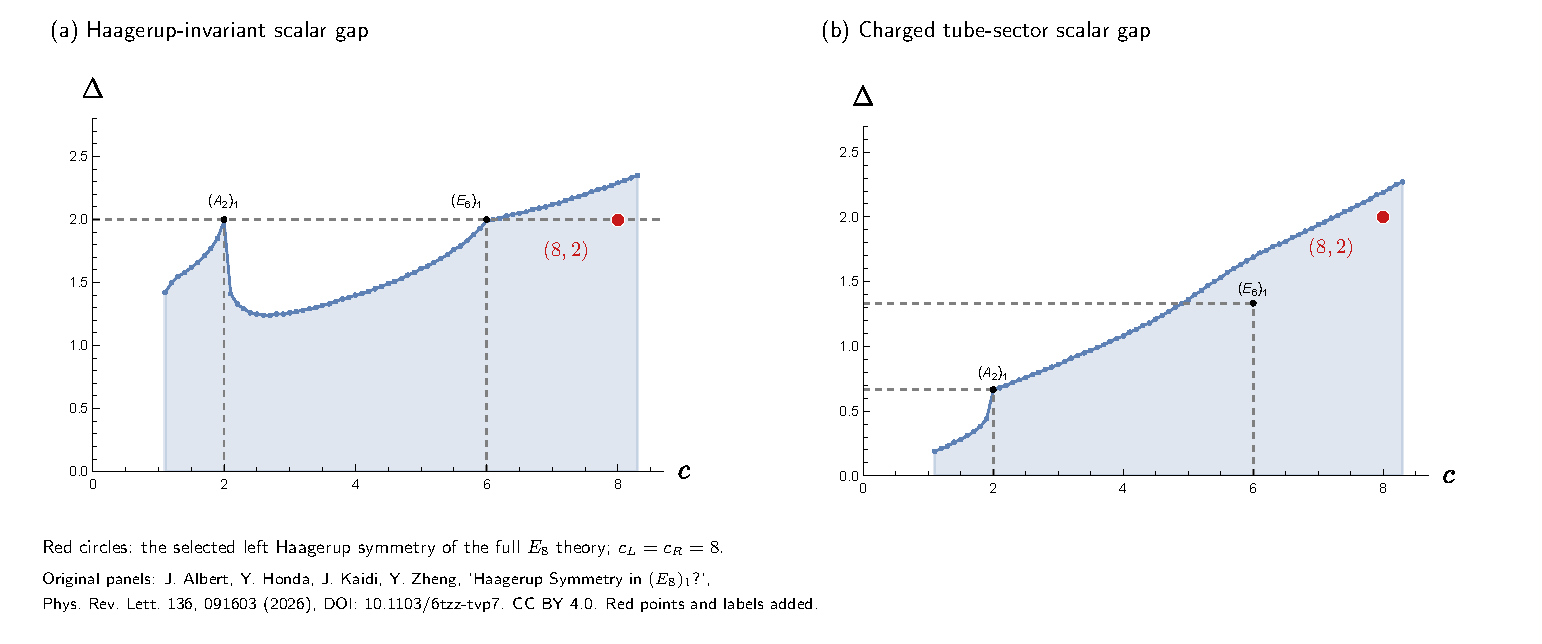
\includegraphics[width=\textwidth]{assets/haagerup_bootstrap_comparison.pdf}
 \caption{The $c_L=c_R=8$ Haagerup comparison points, shown in red.
 Original panels from J.~Albert, Y.~Honda, J.~Kaidi, and Y.~Zheng,
 \emph{Haagerup Symmetry in $(E_8)_1$?}, Phys.~Rev.~Lett.~136,
 091603 (2026), \href{https://doi.org/10.1103/6tzz-tvp7}{doi:10.1103/6tzz-tvp7},
 reproduced under CC~BY~4.0. Red markers and labels have been added.
 The left panel bounds $\mathcal V_1$; the right panel bounds
 $\mathcal V_{\pi_2}\cup\mathcal V_{\sigma_1}$.}
 \label{fig:physics-Haagerup-bootstrap}
\end{figure}

\subsection{Which observables are now supplied}

The release directory \artifact{c8_physics_20260927/} contains plain
TSV tables for inspection and JSON records retaining the algebraic
numbers, basis conventions, and exact derivations. There are four
distinct kinds of evidence.
\begin{enumerate}
 \item The character recurrence supplies complete spin-resolved state
 and Virasoro-primary spectra through $\Delta=24$, for both full
 theories. Thermodynamic intervals add a proved bound on the omitted
 tail, conditional on modular invariance and positivity.
 \item The actual lattice fields supply chiral vacuum-module
 three-point coefficients and the displayed four-point functions.
 Unit normalization and PCT are explicit. The current Ward completion
 of the weight-two tensor is checked against direct additional mode
 calculations.
 \item The positive modular data supply all Verlinde coefficients,
 diagonal-theory line eigenvalues, twisted partition functions and
 Cardy annuli. The selected extension and its free--forgetful
 adjunction supply the Haagerup-resolved $E_8$ sectors and boundaries.
 \item Universal CFT identities then give finite-size energies,
 momenta, entropy coefficients and the stress-tensor and current Ward
 observables. They do not determine the microscopic velocity $v$.
\end{enumerate}

The central unresolved interaction problem is the normalized bulk OPE
of the nonvacuum diagonal sectors, beginning with the nine scalar
components of dimension $2/3$. Neither their character coefficients
nor their fusion multiplicities determine their three-point constants.
An actual lattice intertwiner block, such as the example given above,
is useful input but must still be projected into channels and sewn
with consistent Hermitian pairings to obtain the full diagonal-CFT
four-point function. The corresponding numerical crossing tests,
general defect-junction correlators, and RG endpoints are not claimed
as outputs of this release. These are concrete follow-up calculations,
with the spectrum and normalization data here providing their starting
point.

Each exported number therefore has a mathematical location. Checking a
rational recurrence is separate from proving that its coefficients are
the characters of the constructed VOA; checking a lattice contraction
is separate from proving full-CFT sewing. This separation is intended
to make remaining gaps visible to both physicists and mathematicians.


\appendix
\section{The explicit lattice construction}\label{sec:construction}
\subsection{Lattice, cocycle, and currents}
Use simple lattice vectors indexed \(0,\ldots,7\). The Gram matrix
has diagonal entries two and off-diagonal entries minus one on
\[
 (0,1),(1,2),(2,3),(3,4),(2,5),(6,7),
\]
with all remaining off-diagonal entries zero. Fix the cocycle
\begin{equation}\label{eq:cocycle}
 \epsilon(a,b)=(-1)^{\sum_i a_i b_i+
                      \sum_{i>j}a_i b_jG_{ij}}.
\end{equation}
Write $L=E_6\oplus A_2$ and $\mathfrak h=L\otimes_{\ZZ}\CC$.
The underlying vector space is
\[
 B=S\bigl(\mathfrak h\otimes t^{-1}\CC[t^{-1}]\bigr)
       \otimes\CC_\epsilon[L].
\]
A monomial $h_1(-n_1)\cdots h_r(-n_r)e^\alpha$ has weight
$(\alpha,\alpha)/2+\sum_i n_i$. In particular its weight is a
nonnegative integer. The exponent in \eqref{eq:cocycle} is bilinear
modulo two, and hence defines a normalized two-cocycle. Directly,
\[
 \frac{\epsilon(\alpha,\beta)}{\epsilon(\beta,\alpha)}
       =(-1)^{(\alpha,\beta)},\qquad
 \epsilon(\alpha,-\alpha)=(-1)^{(\alpha,\alpha)/2}.
\]
These identities fix the signs of all root brackets. For example,
$e^\alpha_0e^{-\alpha}=-\alpha(-1)\one$ for a root $\alpha$.
The exponential fields obey
\begin{equation}\label{eq:lattice-product}
 Y(e^\alpha,z)e^\beta
 =\epsilon(\alpha,\beta)z^{(\alpha,\beta)}
   \exp\!\left(\sum_{n>0}\frac{\alpha(-n)}{n}z^n\right)e^{\alpha+\beta}.
\end{equation}
Together with the Heisenberg commutation relations, this formula
specifies the exact mode engine used by the certificates.

Put $\alpha_i=(0,\ldots,1,\ldots,0)$ and
$\alpha_L=(-1,-2,-3,-2,-1,-2,0,0)$. With
\[
 (c_0,\ldots,c_7)=(5,8,9,8,5,0,2,2),\qquad
 h_R=\sum_i c_i\alpha_i,
\]
the two current triples, in the order $(H,E,F)$, are
\begin{align}
 (H_L,E_L,F_L)&=
   (\alpha_L(-1)\one,e^{\alpha_L},-e^{-\alpha_L}),\label{eq:leftcurrents}\\
 (H_R,E_R,F_R)&=
   \left(h_R(-1)\one,\sum_{c_i\ne0}e^{\alpha_i},
                    -\sum_i c_i e^{-\alpha_i}\right).
                    \label{eq:rightcurrents}
\end{align}
Current letters also denote their zero-mode actions when applied to
a state. Thus, for example, $F_RE_Rv$ means
$(F_R)_0(E_R)_0v$.

\begin{lemma}[The two affine levels]\label{lem:levels}
The triples \eqref{eq:leftcurrents}--\eqref{eq:rightcurrents} commute
and generate $A_{1,1}\otimes A_{1,39}$.
\end{lemma}
\begin{proof}
We have $(\alpha_L,\alpha_L)=2$ and
$(\alpha_L,\alpha_i)=0$ whenever $c_i\ne0$.
Also $(h_R,\alpha_i)=2$ for every $c_i\ne0$, and
$(h_R,h_R)=78$. Formula~\eqref{eq:lattice-product} gives
$[H_0,E_0]=2E_0$, $[H_0,F_0]=-2F_0$ and $[E_0,F_0]=H_0$
for both triples. The double poles are
\[
 (H_L)_1H_L=2\one,\quad (E_L)_1F_L=\one,\quad
 (H_R)_1H_R=78\one,\quad (E_R)_1F_R=39\one.
\]
Orthogonality gives all mixed singular products equal to zero.
These are the affine relations at levels one and thirty-nine.
The positive-definite lattice representation is integrable; equivalently
one may use the principal $\mathfrak{sl}_2$ embeddings in $A_5$ and
$A_2$, whose levels $35$ and $4$ add in the diagonal. Thus the
generated factors are the simple positive-integral-level affine VOAs.
Their tensor product is simple and embeds in $B$.
\end{proof}

\subsection{The defining field and the positive real form}
The exact coefficient convention uses unnormalized simple-root
Heisenberg oscillators and a torus gauge in which the principal raising
current is the sum of the corresponding simple-root vertices. The
lowering current is \(-\sum_i c_i e^{-\alpha_i}\), with
\[
 (c_0,\ldots,c_7)=(5,8,9,8,5,0,2,2).
\]
The torus rescales simple-root vertices by
\( (1/\sqrt5,1/\sqrt8,1/3,1/\sqrt8,1/\sqrt5,1,1/\sqrt2,1/\sqrt2)\).
In this convention define
\begin{align}
 u={}&e^{(0,0,0,0,0,-1,1,1)}\notag\\
 &+\frac{\sqrt{13}+3\sqrt{-3}}{20}
                   e^{(0,0,0,1,1,-1,0,0)}\notag\\
 &+\frac{\sqrt{13}-3\sqrt{-3}}{20}
                   e^{(1,1,0,0,0,-1,0,0)}.\label{eq:u}
\end{align}
The compact real form and PCT operation must be transported through
this gauge. Ordinary coefficient conjugation in the displayed gauge
is not a replacement for the ambient PCT map.

Here is the transport explicitly. Set
$\widetilde c=(5,8,9,8,5,1,2,2)$ and let $g$ be the lattice torus
automorphism which fixes the oscillators and multiplies $e^\alpha$ by
$\prod_i\widetilde c_i^{-\alpha_i/2}$. If $\theta$ is the ordinary
lattice PCT involution, the transported involution is
$\theta_g=g\theta g^{-1}$. For real lattice oscillators,
\begin{equation}\label{eq:pct}
 \theta_g\bigl(h_1(-n_1)\cdots h_r(-n_r)e^\alpha\bigr)
 =(-1)^r\Bigl(\prod_i\widetilde c_i^{\alpha_i}\Bigr)
       h_1(-n_1)\cdots h_r(-n_r)e^{-\alpha}.
\end{equation}
It acts antilinearly on coefficients, so fixes $\sqrt{13}$ and
negates $\sqrt{-3}$. The transported Hermitian form is
$\langle v,w\rangle_g=\langle g^{-1}v,g^{-1}w\rangle$ and is
positive definite. Formula~\eqref{eq:pct} squares to the identity.
The same torus element acts on $V_{E_8}$: the positive real character
on $L$ extends by its real linear logarithm to the common Cartan space.
We transport the form and PCT on $H$ by that element as well, so the
entire inclusion $U\subset B\subset H$ uses one unitary convention.
It preserves the current algebra, including the root factor even
though its two root vectors have different norms in this gauge.

All three momenta in \eqref{eq:u} have squared norm four and Cartan
weight $(1,13)$. Substitution in the lattice formula verifies that
$u$ is a highest vector of current type $(2,14)$, where the entries
now denote representation dimensions. In the original positive unitary
basis, $g^{-1}u$ is, up to a common scalar,
\[
 e^a+\zeta e^b+\overline\zeta e^c,\qquad
 \zeta=\frac{\sqrt{13}+3i\sqrt3}{\sqrt{40}},\qquad |\zeta|=1,
\]
with $a,b,c$ the three displayed momenta. Thus the exact construction
fixes a relative phase; there is no remaining continuous parameter.

The ambient and affine conformal vectors are fixed by these conventions:
\begin{align}
 \omega_B&=\frac12\sum_{i,j}(G^{-1})_{ij}
               \alpha_i(-1)\alpha_j(-1)\one,\label{eq:ambient-stress}\\
 \omega_{A_{1,k}}&=\frac{1}{2(k+2)}
       \left(\tfrac12 H_{-1}H+E_{-1}F+F_{-1}E\right).
       \label{eq:sugawara}
\end{align}
The conformal vector of $U$ is $\omega_B$, not the sum of the two
affine conformal vectors. Their central charges sum to
$1+117/41<8$.

\subsection{The constructed spaces in weights two and three}

\begin{certificate}[Actual initial spaces]\label{cert:initial}
The saved exact construction gives a PCT-stable 120-dimensional
space \(S_2\subset U_2\), containing \(u,\omega_B\), the affine
vacuum descendants, two neutral primitive fields, and eight charged
current multiplets. The current multiplet dimensions are
\[
 (1,5),(1,9),(1,9),(1,13),(2,2),(2,6),(2,8),(2,14).
\]
These contribute 96 vectors, in addition to the 22 affine vacuum
vectors and two neutral fields. The exact generated grade-three
space \(S_3\subset U_3\) has dimension 956. Its normal subspace
\(N_3=K_{-1}S_2+TS_2\) has dimension 634, and
\[
 S_3=N_3+\Span\{a_0b:a,b\in S_2\},\qquad \dim(S_3/N_3)=322.
\]
The spaces are current-stable. These are dimensions of constructed
finite spaces, not initial assertions that they exhaust \(U_2,U_3\).
\end{certificate}
The source records are
\artifact{hi_cft_20260923_c8_exact_fields.json},
\artifact{hi_cft_20260923_c8_exact_unitary_certificate.json}, and
\artifact{hi_cft_20260923_c8_minimal_generators.json}, together with
the exact grade-three checkpoint bound into the final ledger.

The minimal-generator record is logically prior to the closure records.
It starts with the six specified currents, $\omega_B$, and $u$, then
closes their weight-two span under current zero modes and $u_1$.
Every intermediate vector is therefore an actual $U$-vector. The final
span has dimension $120$ and contains each independently specified
highest vector and neutral conformal vector. The equality with the saved
space $S_2$ is checked only after this construction. This is the step
that relates the large certificate presentation to the short definition
\eqref{eq:U}; an ambient weight-two dimension count alone would not do so.

For reference the two neutral fields, denoted $e,f$, satisfy
\begin{equation}\label{eq:two-coset-stresses}
 e+f=\omega_B-\omega_{A_{1,1}}-\omega_{A_{1,39}},\qquad
 c_e=\frac{2400}{1271},\quad c_f=\frac{70}{31}.
\end{equation}
They commute as Virasoro fields. The exact current and stress
eigenvalues on the eight primitive highest vectors are as follows.
The two occurrences of $(1,9)$ are distinct vectors.
\begin{center}
\begin{tabular}{@{}ccc@{}}
\toprule
Current dimensions $(n,m)$ & $e_1$ eigenvalue & $f_1$ eigenvalue\\
\midrule
$(1,5)$ & $798/1271$ & $38/31$\\
$(1,9)$ & $200/1271$ & $42/31$\\
$(1,9)$ & $1512/1271$ & $10/31$\\
$(1,13)$ & $420/1271$ & $20/31$\\
$(2,2)$ & $192/1271$ & $49/31$\\
$(2,6)$ & $1830/1271$ & $3/31$\\
$(2,8)$ & $752/1271$ & $24/31$\\
$(2,14)$ & $180/1271$ & $13/31$\\
\bottomrule
\end{tabular}
\end{center}
Each row obeys
\[
 \frac{n^2-1}{12}+\frac{m^2-1}{164}+h_e+h_f=2.
\]
The affine vacuum space contributes $22$ dimensions in weight two:
$4$ from $A_{1,1}$, $9$ from $A_{1,39}$, and $3\cdot3$ mixed
current products. The level-one null multiplet removes five of the
nine universal weight-two states of its affine factor. Together with
the two singlets and the $96$ charged states, this gives $120$.
The exact normal-space and rank calculations certify these spaces
inside the lattice algebra, including their intersections.

\section{Finite closure and the all-weight criterion}\label{sec:finite}
Write \(Y(a,z)=\sum_{n\in\ZZ}a_nz^{-n-1}\) and \(T=L(-1)\).
A singular product has mode index \(n\geq0\). The zero mode \(a_0\)
is a derivation and commutes with \(T\).

\begin{definition}[Differential normal span]\label{def:normal-span}
For a homogeneous positive-weight subspace $S\subset V$, let
$\mathcal N(S)$ be the linear span of the vacuum and every expression
obtained from vectors of $S$ by translation and arbitrary parenthesized
$(-1)$ products. Let $\mathcal N_d(S)=\mathcal N(S)\cap V_d$.
This definition makes translation and normal multiplication closed
operations on $\mathcal N(S)$; closure under singular products is a
separate assertion. We use the usual convention that a set strongly
generates when its differential normal span is the whole algebra.
\end{definition}

\begin{lemma}[Filtered Wick reduction]\label{lem:filtered-wick}
Let $V$ be a nonnegatively integer-graded vertex algebra with
$V_0=\CC\one$, and let $S$ have strictly positive weights. Fix $w$.
Suppose every singular product of two homogeneous generators of total
weight less than $w$ belongs to $\mathcal N(S)$. Then the same is
true for two normal expressions of total weight less than $w$.
It is also true at total weight $w$ if at least one expression is a
derivative of a positive-weight expression or a normal product of
two positive-weight expressions.
\end{lemma}
\begin{proof}
Use induction on total input weight. A vacuum factor has zero singular
bracket. Sesquilinearity removes a derivative and lowers the total input
weight; the resulting powers of the formal variable and translations
preserve coefficientwise membership in $\mathcal N(S)$. Skew symmetry
allows a composite input to be placed on the right. The noncommutative
Wick identity is
\begin{equation}\label{eq:wick}
 [x_\lambda:y z:]=:[x_\lambda y]z:+:y[x_\lambda z]:
             +\int_0^\lambda [[x_\lambda y]_\mu z]\,d\mu.
\end{equation}
The first two brackets have smaller total input weight, since an
omitted factor has positive weight. Their coefficients therefore admit
homogeneous expressions in $\mathcal N(S)$. A coefficient $x_jy$ in
the integral has weight $\wt(x)+\wt(y)-j-1$. Its pairing with $z$
has total weight at most $\wt(x)+\wt(y)+\wt(z)-1$, so induction
applies again. If the coefficient is scalar, its bracket is zero.
Normal multiplication preserves the first two terms by definition.
This proves both assertions, including the case in which both inputs
are composite. Neither a preferred parenthesization nor independence
of normal words was used.
\end{proof}

\begin{theorem}[Recursive strong-generation criterion]\label{thm:recursive}
Let \(V\) be a nonnegatively graded vertex algebra with \(V_0=\CC\one\).
Choose finite homogeneous subspaces \(S_d\subset V_d\),
\(1\leq d\leq h\), where $h\geq2$, and let \(\mathcal N\) be their differential
normally ordered span, allowing every parenthesization. Put
\(K=S_1\) and \(A=S_2\). Assume
\begin{enumerate}
\item \(k_ns,a_ns\in\mathcal N\) for every \(k\in K\), \(a\in A\),
\(s\in S_d\), and \(n\geq0\);
\item for \(d\geq3\),
\[
 S_d\subset A_0S_{d-1}+\mathcal N_d(S_1+\cdots+S_{d-1}).
\]
\end{enumerate}
Then \(\mathcal N\) is a vertex subalgebra. In particular, the chosen
spaces strongly generate the vertex algebra that they generate.
\end{theorem}

\begin{proof}
The first assumption, the derivation property and \([T,a_0]=0\)
give \(a_0\mathcal N\subset\mathcal N\) for \(a\in A\).
Explicitly, $a_0(x_{-1}y)=(a_0x)_{-1}y+x_{-1}(a_0y)$, so
induction on the construction of a normal expression proves this
stability before any singular-product closure is known.

Now induct lexicographically on
\((\wt(s)+\wt(t),\wt(s))\) for generator pairs \(s,t\).
Left weight one or two is the first assumption. Otherwise the second
assumption reduces the left input to \(s=a_0b\), with
\(\wt(b)=\wt(s)-1\), plus normal remainders. The latter are covered
by Lemma~\ref{lem:filtered-wick}: a homogeneous remainder of weight
$\wt(s)$ in lower-weight generators has no single undifferentiated
generator of that weight. Use
\begin{equation}\label{eq:recursive-jacobi}
 (a_0b)_nt=a_0(b_nt)-b_n(a_0t).
\end{equation}
The first term has smaller total pair weight before applying \(a_0\),
which preserves \(\mathcal N\). The known normal expression for
\(a_0t\) has weight \(\wt(t)+1\). Every derivative or composite term
reduces total pair weight in the second term. The only remaining
possibility is a single undifferentiated generator of weight
\(\wt(t)+1\); its pairing with \(b\) has the original total weight
and smaller left weight. It is therefore an earlier induction case.
If \(\wt(t)=h\), this single-generator possibility is absent.

All generator singular products close. Wick induction then gives closure
for all normal expressions. Translation and normal multiplication
preserve \(\mathcal N\) by definition. For $r\geq1$,
\[
 x_{-r}y=\frac{1}{(r-1)!}(T^{r-1}x)_{-1}y,
\]
so all negative modes close too.
\end{proof}
For the Wick identities see \cite[Section 2]{DSK}.
The full local derivation is
\artifact{hi_cft_20260923_next_structure_recursive_strong_certificate.md}.

\begin{remark}[Finite scope of the input]\label{rem:finite-scope}
Every membership in the first hypothesis has output weight at most
$h+1$. Thus the criterion avoids checking all generator pairs through
weight $2h-1$. The second hypothesis is essential: it asserts actual
zero-product identities, rather than agreement of a dimension or a
character coefficient. The proof takes place in the given ambient
vertex algebra and makes no assertion that its normal words are free.
This resolves the all-weight implication formerly marked F2.
\end{remark}

\subsection{The finite spaces and prerequisite controls}
Choose actual quotient lifts \(P_3\subset S_3\) and an actual triplet
\(P_4\subset U_4\), with joint current highest weight \((0,2)\), and set
\begin{align}
 N_4&=K_{-1}S_3+TS_3+(S_2)_{-1}S_2,&W_4&=N_4+P_4,\label{eq:normal4}\\
 N_5&=K_{-1}W_4+TW_4+(S_2)_{-1}S_3.&&\label{eq:normal5}
\end{align}
These denote full differential normal spaces, using the lower closure
identities to reorder expressions. A computational solver may use a
proper subset of actual words in these spaces.

The triplet is obtained from an actual \(a_0p\) by current-zero-mode
projectors and lowering. It satisfies
\(P_4\subset (S_2)_0S_3+N_4\).

\begin{lemma}[Bounds for the current projectors]\label{lem:current-bounds}
On ambient weight $d$, a Cartan element represented by $h\in L\otimes\mathbb R$
has eigenvalues $m$ satisfying $m^2\leq2d(h,h)$. At weight four
the two current highest weights are therefore at most $4$ and $24$.
\end{lemma}
\begin{proof}
Cartan zero modes act on a Fock monomial of momentum $\alpha$ by
$(h,\alpha)$, and commute with its oscillators. The grading gives
$(\alpha,\alpha)\leq2d$, so the estimate is Cauchy--Schwarz in the
positive lattice form. Every eigenvalue is integral. Apply the estimate
to $(h,h)=2,78$ and $d=4$, and then to the highest vectors in the
finite-dimensional semisimple current decomposition.
\end{proof}

Consequently finite polynomials in \(FE\) give exact projectors.
For an input of weight \((0,2)\), one may use
\[
 \prod_{\ell=1}^{2}\left(1-\frac{F_LE_L}{\ell(\ell+1)}\right),
 \qquad
 \prod_{\ell=2}^{12}\left(1-\frac{F_RE_R}{\ell(\ell+1)-2}\right).
\]
The raising operator acts first in every \(FE\) factor.
Indeed, on the weight-$m$ line in an $\mathfrak{sl}_2$ representation
of highest weight $j$, $FE$ acts by $(j-m)(j+m+2)/4$. The first
polynomial retains left highest weight zero. At right weight two the
second retains highest weight two and kills every possible larger
highest weight. Thus all denominators are nonzero and the projector
has a finite, justified range.

\begin{certificate}[Lower identities and the actual triplet]\label{cert:lower}
The lower-closure artifact contains 3,970 completed exact identities.
The actual \(P_4\) vectors satisfy 18 current-zero-mode identities and
six independently checked inclusions
\[
 L(1)P_4\subset S_3,\qquad L(2)P_4\subset S_2.
\]
These direct Virasoro checks are available before the weight-four gate.
\end{certificate}
The two gates left for the all-weight argument are
\begin{align}
 (S_2)_0S_3&\subset W_4 &&\text{(Gate 4)},\label{eq:gate4}\\
 (S_2)_0P_4&\subset N_5 &&\text{(Gate 5)}.\label{eq:gate5}
\end{align}

\section{Gate 4: exact seeds, raising, and singlet recovery}\label{sec:gate4}
Put \(P=S_3/N_3\), of independently known dimension 322. For a fixed
joint-highest primitive field \(a\in S_2\), the map
\[
 f_a:P\longrightarrow B_4/W_4,\qquad [p]\longmapsto[a_0p]
\]
is well defined because the lower relations give \(a_0N_3\subset N_4\).
Current covariance implies that its kernel is stable under both commuting
raising operators \(E_L,E_R\).

\begin{lemma}[Raising saturation]\label{lem:raising}
If \(C_a\subset\ker f_a\) and
\(P=E_LP+E_RP+C_a\), then \(f_a=0\).
\end{lemma}
\begin{proof}
On \(M=P/\ker f_a\) the hypothesis says
\(M=E_LM+E_RM\). The commuting ideal \((E_L,E_R)\) acts nilpotently
because all current weights are bounded. Iterating gives
\(M=(E_L,E_R)^rM=0\) for sufficiently large \(r\).
\end{proof}

In this application nilpotence is entirely finite-dimensional. At weight
three Lemma~\ref{lem:current-bounds} bounds the two Cartan eigenvalues
by $|m_L|\leq3$ and $|m_R|\leq21$. Either raising operator increases
$m_L+m_R$ by two. Every word of length $25$ in the two raising
operators therefore vanishes on $P$. The quotient by $\ker f_a$
inherits these operators because the kernel is stable. This gives an
explicit termination bound for the argument; there is no limiting step.

The exact raising coordinates comprise 644 images. Their rank is 294.
For each of nine independent highest left fields, the completed seed
sets and these images have rank 322. A nonzero minor at the good split
prime \(p=1{,}000{,}003\) proves a nonzero characteristic-zero minor.
This proves spanning because the exact ambient quotient dimension is
already 322. It does not give an upper rank for an unknown weight-four
normal space.

The original exact run supplies 2,145 seed identities. The saturation
calculation asks for 130 further inputs; 118 have direct exact residual
certificates. The remaining twelve outputs have weight \((0,0)\).
An exact replay of the known kernel and twelve additional identities
at output weight \((0,2)\) shows that both raising currents kill each
of these twelve remaining classes modulo \(W_4\).

\begin{lemma}[Recovery from a joint-singlet projection]\label{lem:singlet}
Let \(t\in B_4\) have weight \((0,0)\), with
\(E_Lt,E_Rt\in W_4\). Define
\begin{equation}\label{eq:projector}
 \Pi=\prod_{j\in\{2,4\}}
       \left(1-\frac{4F_LE_L}{j(j+2)}\right)
       \prod_{j\in\{2,4,\ldots,24\}}
       \left(1-\frac{4F_RE_R}{j(j+2)}\right).
\end{equation}
If \(\Pi t\) is a linear combination of \(\Pi n_i\), with
\(n_i\in N_4\), then \(t\in W_4\).
\end{lemma}
\begin{proof}
Both \(W_4\) and \(N_4\) are stable under current zero modes.
Every \(FE\) factor kills \([t]\in B_4/W_4\), so
\([\Pi t]=[t]\). Each \(\Pi n_i\) remains in \(N_4\subset W_4\).
Thus \([t]=0\). Equivalently, the weight-zero highest class is a singlet
in the finite semisimple current module. No dimension assertion about
the selected normal columns is needed.
\end{proof}

The prime search selects 21 independent projected normal columns.
All twelve projected identities have complete residual zero over
\(\QQ(\sqrt{13},\sqrt{-3})\). The final verifier repeats those
residuals by independent integer denominator clearing, authenticates
the raising premise, and repeats all nine saturation ranks. By
Lemmas~\ref{lem:raising} and~\ref{lem:singlet}, all \(9\cdot322=2898\)
required highest-left identities hold. Current covariance gives the
charged descendants. The second neutral field follows from
\(\omega_B-\omega_{K_L}-\omega_{K_R}\) minus the retained neutral field.
This proves \eqref{eq:gate4} with the certified lower controls.

\subsection{Positive modes available after Gate 4}
\label{sec:bootstrap}
The normal-product argument at the next gate uses positive modes on
$S_3$. We establish them here, before their first use. This also explains
why no additional unverified positive-mode gate is required.

\begin{lemma}[Virasoro and current bootstrap]\label{lem:bootstrap}
The lower identities, the direct $P_4$ controls, and Gate~4 imply
\begin{align}
 (S_2)_1S_3&\subset S_3,& (S_2)_2S_3&\subset S_2,&
 (S_2)_3S_3&\subset K,\label{eq:positive-S3}\\
 K_1W_4&\subset S_3,&K_2W_4&\subset S_2,&K_3W_4&\subset K,
 \label{eq:positive-W4}\\
 L(1)N_5&\subset W_4,&L(2)N_5&\subset S_3.&&
 \label{eq:positive-N5}
\end{align}
The next mode in each of the first two lines is scalar, and all further
modes vanish.
\end{lemma}
\begin{proof}
The exact lower inputs give all singular products of $K$ and $S_2$
with $S_2$ in the expected lower spaces. The provenance
$S_3=N_3+(S_2)_0S_2$ and the current commutator give
\[
 K_0S_3\subset S_3,\qquad K_1S_3\subset S_2,\qquad
 K_2S_3\subset K.
\]
For instance,
\begin{equation}\label{eq:k1-provenance}
 k_1(a_0b)=(k_0a)_1b+(k_1a)_0b+a_0(k_1b).
\end{equation}
The Virasoro commutators for a weight-two vector are
\begin{align}
 [L(1),a_n]&=(2-n)a_{n+1}+(L(1)a)_n,\label{eq:L1-weight2}\\
 [L(2),a_n]&=(3-n)a_{n+2}+3(L(1)a)_{n+1}+(L(2)a)_n.
 \label{eq:L2-weight2}
\end{align}
They show $L(1)S_3\subset S_2$ and $L(2)S_3\subset K$.
Applied to the three summands of $N_4$, they give
$L(1)N_4\subset S_3$ and $L(2)N_4\subset S_2$.
For a normal input $a_{-1}b$ the latter formula includes the scalar
term $(L(2)a)_{-1}b$; it must not be omitted. It lies in $S_2$.
The six direct controls of Certificate~\ref{cert:lower} extend these
inclusions to $W_4$ without using Gate~5.

Each of the eight charged primitive multiplets and the two neutral
singlets in $S_2$ is quasiprimary. Indeed, $L(1)$ is equivariant for
current zero modes, and none of their current types is $(3,1)$ or
$(1,3)$, the two types in $K$. For such a vector $a$ and $p\in S_3$,
Gate~4 and the preceding controls give
\begin{align*}
 2a_1p&=L(1)(a_0p)-a_0L(1)p\in S_3,\\
 a_2p&=L(1)(a_1p)-a_1L(1)p\in S_2,\\
 2a_3p&=L(2)(a_1p)-a_1L(2)p\in K.
\end{align*}
In the last line the possible $(L(2)a)_1$ term is zero since $L(2)a$
is scalar. The affine normal and derivative part of $S_2$ is handled
by the current iterate identities. This proves
\eqref{eq:positive-S3} on all of $S_2$.

The actual construction gives $P_4\subset(S_2)_0S_3+N_4$.
Equation~\eqref{eq:k1-provenance}, now with $b\in S_3$, gives
$K_1P_4\subset S_3$; the same inclusion for $N_4$ follows on its
normal generators. Since currents are primary of weight one,
\[
 [L(1),k_1]=-k_2,\qquad [L(2),k_1]=-k_3.
\]
The controls on $L(1)W_4,L(2)W_4$ consequently give
\eqref{eq:positive-W4}. The remaining modes follow from grading.

Finally apply $L(1),L(2)$ to
$N_5=K_{-1}W_4+TW_4+(S_2)_{-1}S_3$. The current and translation
summands follow from the established inclusions and the Virasoro
relations. For the third summand, the required formulas are
\begin{align*}
 L(1)(a_{-1}p)
 &=3a_0p+(L(1)a)_{-1}p+a_{-1}L(1)p,\\
 L(2)(a_{-1}p)
 &=4a_1p+3(L(1)a)_0p+(L(2)a)_{-1}p+a_{-1}L(2)p.
\end{align*}
Every term belongs respectively to $W_4$ or $S_3$ by Gate~4,
\eqref{eq:positive-S3}, and the lower identities. Reordering the last
normal term uses only already established lower products. This proves
\eqref{eq:positive-N5}.
\end{proof}

\section{Gate 5 from Jacobi identities}\label{sec:gate5}
The proof uses the full normal spaces in
\eqref{eq:normal4}--\eqref{eq:normal5}, not only the selected solver
columns. To see that the displayed formula for $N_5$ includes every
lower normal word of weight five, remove a leading derivative, or
split a normal product into weights $1+4$ or $2+3$. Reversed splits
are reordered by skew symmetry for normal products. Its correction
terms are derivatives of singular products, already controlled by
Lemma~\ref{lem:bootstrap} and the lower identities. Quasi-associativity
changes the parenthesization with correction terms of the same type.
Thus the resulting words lie in
$K_{-1}W_4+TW_4+(S_2)_{-1}S_3$.

\begin{lemma}[Normal-space controls]\label{lem:normal-controls}
Before using Gate 5, the lower controls and Gate 4 give
\begin{equation}\label{eq:normal-lemmas}
 (S_2)_0N_4\subset N_5,\qquad (N_3)_0S_3\subset N_5.
\end{equation}
\end{lemma}
\begin{proof}
The first follows by zero-mode derivation and skew reordering. For the
second, \((Ta)_0=0\) and, for a current \(x\),
\begin{equation}\label{eq:iterate}
 (x_{-1}a)_0p
 =\sum_{i\geq0}x_{-1-i}(a_ip)
  +\sum_{i\geq0}a_{-1-i}(x_ip).
\end{equation}
All inner products belong to the required lower spaces. To make the
translation reduction explicit, repeatedly use
\[
 x_{-r}v=\frac{T(x_{-(r-1)}v)-x_{-(r-1)}Tv}{r-1},\qquad r\geq2.
\]
The base terms are precisely those in \eqref{eq:normal5}; the same
identity applies to \(a_{-r}v\) with \(a\in S_2\). Thus no
unproved \(P_3\)-by-\(P_3\) closure enters \eqref{eq:normal-lemmas}.
All positive inner modes in \eqref{eq:iterate} are supplied by
\eqref{eq:positive-S3} and the current controls established before
this section. More explicitly the first sum has inner vectors in
$W_4,S_3,S_2,K,\CC\one$, in that order; the second has inner
vectors in $S_3,S_2,K,\CC\one$. Both sums are finite by grading.
\end{proof}

If \(P_4\subset N_4\), Gate 5 already follows. Otherwise
\(Q=W_4/N_4\) is the irreducible current triplet of highest weight
\((0,2)\), since the actual \(P_4\) is irreducible. Let
\(q_-,q_0,q_+\) be its weight basis, and set
\[
 \beta(a,p)=[a_0p]\in Q,\qquad
 F(a,q)=[a_0\widetilde q]\in B_5/N_5.
\]
The second map does not depend on the representative
\(\widetilde q\in W_4\), by \eqref{eq:normal-lemmas}.

\begin{lemma}[Jacobi reduction]\label{lem:jacobi}
If \(a,b\in S_2\) satisfy \(a_0b\in N_3\), then for \(p\in S_3\),
\begin{equation}\label{eq:jacobi-reduction}
 F(a,\beta(b,p))=F(b,\beta(a,p)).
\end{equation}
\end{lemma}
\begin{proof}
The difference is the class of \((a_0b)_0p\), which vanishes by
\eqref{eq:normal-lemmas} and \([a_0,b_0]=(a_0b)_0\).
\end{proof}

\subsection{The charged families}
Let \(a_0,\ldots,a_7\) denote the eight charged highest fields, with
current weights
\[
 (0,4),(0,8),(0,8),(0,12),(1,1),(1,5),(1,7),(1,13).
\]
In a product such as \((a_i)_0p\), the parenthesized subscript denotes
the field label and the next subscript denotes its mode.
The saved exact relations give
\[
 \beta(a_3,p_3)=c_3q_-,\qquad \beta(a_6,p_6)=c_6q_-,
 \qquad c_3c_6\neq0,
\]
where \(p_3=\texttt{r3\_000910}\) has weight \((0,-14)\), and
\(p_6=\texttt{r3\_000899}\) has weight \((-1,-9)\).
The coefficients are authenticated in the final Jacobi certificate.
Exact combinations of the lower relations establish \((a_i)_0a_j\in N_3\)
for the following pairs:
\begin{center}
\begin{tabular}{@{}cccl@{}}
\toprule
\(i\)&\(j\)&Input&Weight of \((a_i)_0p_j\)\\
\midrule
0&3&\(p_3\)&\((0,-10)\)\\
1,2&3&\(p_3\)&\((0,-6)\)\\
3&6&\(p_6\)&\((-1,3)\)\\
4&6&\(p_6\)&\((0,-8)\)\\
5&3&\(p_3\)&\((1,-9)\)\\
6&3&\(p_3\)&\((1,-7)\)\\
7&3&\(p_3\)&\((1,-1)\)\\
\bottomrule
\end{tabular}
\end{center}
Every listed output weight lies outside \(Q\), so
\(\beta(a_i,p_j)=0\). Equation~\eqref{eq:jacobi-reduction} and
\(c_j\neq0\) give \(F(a_i,q_-)=0\). Raise this resulting zero
with \(a_i\) held highest to obtain the other two right inputs.
Current covariance gives all left descendants.

\begin{remark}
The weight exclusion is used only at the displayed bottom inputs.
It need not hold after raising \(p_j\); using it there would be an
incorrect stronger assertion. We raise the proved zero identity instead.
\end{remark}

\subsection{The neutral family}
Let \(C\) be the full current span, inside \(P=S_3/N_3\), of
brackets of charged weight-two fields. The charged-span certificate
reconstructs 28 actual charged seeds from the exact lower relations.
Together with the 644 lowering images, of rank 294, these have rank 322.
The independent verifier also checks both \(\mathfrak{sl}_2\) commutators
and all cross-axis commutators against the saved exact raising matrices.
Since \(C\) is a current submodule, the nilpotent-ideal argument gives
\[
 P=F_LP+F_RP+C\quad\Longrightarrow\quad P/C=0.
\]
Once again the finite-prime full rank is a positive spanning witness
inside an independently exact 322-dimensional space.

For the retained neutral singlet \(e\), write
\[
 e_0a_3=\sum_i t_i(x_i)_0y_i+n,
 \qquad n\in N_3,
\]
with charged \(x_i,y_i\). Apply zero modes to \(p_3\). By Jacobi,
the charged conclusion and \eqref{eq:normal-lemmas},
\[
 (e_0a_3)_0p_3
 =\sum_i t_i[(x_i)_0,(y_i)_0]p_3+n_0p_3\in N_5.
\]
Indeed Gate 4 puts each inner product in \(W_4\), and the next charged
product is controlled on both \(N_4\) and \(P_4\). A second Jacobi
identity gives
\[
 e_0((a_3)_0p_3)=(a_3)_0(e_0p_3)+(e_0a_3)_0p_3\in N_5.
\]
The nonzero coefficient of \(q_-\) proves the neutral bottom identity;
covariance gives the triplet. The other neutral field is obtained from
the total stress minus the two affine Sugawara stresses and \(e\).
This proves Gate 5. Its 24 independent highest channels comprise
23 charged channels and one neutral channel; they are consequences
of the displayed identities, not 24 separately recomputed grade-five
lattice products.

\section{From the finite gates to properness}\label{sec:properness}
Lemma~\ref{lem:bootstrap} supplies the positive-current products and
$L(1)N_5\subset W_4$, $L(2)N_5\subset S_3$ before Gate~5.
For a quasiprimary primitive $a\in S_2$,
Gate 5 now yields, for \(p\in P_4\),
\begin{align*}
 2a_1p&=L(1)(a_0p)-a_0L(1)p\in W_4,\\
 a_2p&=L(1)(a_1p)-a_1L(1)p\in S_3,\\
 2a_3p&=L(2)(a_1p)-a_1L(2)p\in S_2,\\
 a_4p&=L(2)(a_2p)-a_2L(2)p\in K.
\end{align*}
The next mode is scalar. The 30 earlier prime-only \(a_1P_4\)
tests are therefore derived exactly here; they are not an omitted gate.

All hypotheses of Theorem~\ref{thm:recursive} hold for
\(K,S_2,S_3,P_4\). Their normal span is a vertex subalgebra of \(U\)
containing \(K,u,\omega_B\), hence equals \(U\). A normal word in
positive-weight generators cannot acquire weight one unless it is a
weight-one generator. Thus \(U_1=K\), proving
Proposition~\ref{prop:mainproper}.

\begin{proof}[Proof of Corollary~\ref{cor:initial-grades}]
A differential normal word of weight two uses only $K$ and $S_2$;
its current descendants are already in $S_2$. A word of weight three
uses only $K,S_2,S_3$, and the lower normal words lie in $N_3$.
Thus the strong-generation result proves $U_2=S_2$ and $U_3=S_3$.
The exact PCT certificate gives $\theta_gS_2=S_2$, while
$\theta_gK=K$. Since $S_2\subset U$ contains the original generators,
$\theta_gU=U$. The inherited positive form makes $U$ a unitary
subalgebra of $B$, hence simple by \cite[Proposition 5.29]{CKLW}.
It contains $\omega_B$, so has central charge eight, the same
nonnegative grading, and $U_0=\CC\one$. The character assertion is
now the definition of the graded trace.
\end{proof}

\begin{reviewnote}{F1: what the finite certificate establishes}
This proof of properness has the strongest computational support in the
manuscript. It still relies on correctness of the lattice mode engine,
the saved actual-vector recipes, and the stated algebraic lemmas.
Hashes authenticate the records; hashes alone do not prove those lemmas
or independently reconstruct every earlier mode calculation. The Lean
checks in Appendix~\ref{sec:formalization} cover selected abstract
implications, not the VOA construction or the complete strong-generation
argument. No second implementation of the entire construction is
claimed. In particular, \(\dim U_4=6010\) is not used as an input to
this proof.
\end{reviewnote}

% Fragment: regularity, branching, fusion-ring reduction, and characters.
% The main document supplies theorem environments, reviewnote, and artifact.

\section{Regularity from a positive conformal-vector identity}
\label{sec:regularity}

This section concerns the actual PCT-stable subalgebra $U\subset B$ defined
in the construction. Its conclusions do not require properness. We use
the convention $Y(a,z)=\sum_{n\in\mathbb Z}a_nz^{-n-1}$ and write
$L^e(n)=e_{n+1}$ for the Virasoro operators of a conformal vector $e$.
The subalgebras used below need not contain the ambient conformal vector.
We call an inclusion $A\subset V$ \emph{grading compatible} if the
$A$-weight of each homogeneous vector of $A$ equals its $V$-weight.
Thus a mode $a_n$ changes both gradings by $\operatorname{wt}(a)-n-1$;
the equality of the two energy operators is not required on all of $V$.
All subalgebras in the positive identity below are grading compatible
and stable under the ambient PCT involution.

\begin{certificate}[Embedded structural data]
\label{cert:structural-inputs}
The following are assertions about actual fields and their exact modes
in the lattice construction, in addition to the finite closure ledger.
\begin{enumerate}
\item The Potts fields lie in $U$, are PCT stable, and generate the
regular unitary algebra $K(\mathfrak{sl}_2,3)$, with its translation
and intrinsic grading inherited from the ambient VOA. The exact
records are \artifact{hi_cft_20260923_proof_potts.json} and
\artifact{hi_cft_20260923_proof_potts_exact.json}.
\item The actual fields $z,a$ of weights two and three lie in $U$,
are PCT stable, have central charge $8/5$, and satisfy the stress,
primary, and translation identities in
\artifact{hi_cft_20260923_proof_pf13_exact.json},
\artifact{hi_cft_20260923_proof_pf13_membership.json}, and
\artifact{hi_cft_20260923_proof_remaining_coset.json}.
Their full singular first rows agree with the parafermion rows at
$c=8/5$, $\lambda=14/473$, as polynomials in $z,a,a_1a,a_1(a_1a)$.
The polynomial records are
\artifact{hi_cft_20260923_proof_pf13_upper_poles.json},
\artifact{hi_cft_20260923_proof_pf13_nonlinear.json},
\artifact{hi_cft_20260923_proof_pf13_truncation.json},
\artifact{hi_cft_20260923_proof_pf13_simple_pole_algebra.json}, and
\artifact{hi_cft_20260923_proof_pf13_dly.json}.
The membership record also gives the positive identity
\eqref{eq:positive-stress}.
\item The lattice--Potts core $T$ below is embedded with its stated
charge realization. The six joint spectral vectors used to construct
its order-thirteen extension are actual vectors of $U_2$, with the
eigenvalues printed below. Their exact source is
\artifact{hi_cft_20260923_next_structure_core_extension.json}; the
construction of $T$ is described in
\artifact{hi_cft_20260923_proof_report.md}, Section~4.
\item The zero-mode action on the complementary eighty currents is
irreducible, and the four mixed lattice tops of dimension eighty-one
are irreducible as $U$-tops. These are exact
field-action assertions, as recorded in
\artifact{hi_cft_20260923_proof_current_module_v2.json} and
\artifact{hi_cft_20260923_next_81top_all.json}, respectively.
\end{enumerate}
All polynomial equalities here mean exact vector equalities in the
fixed lattice realization, not projected or floating-point matches.
\end{certificate}

The input from the local construction is the identity
\begin{equation}
 \omega_U=\omega_{A_{1,1}}
   +\frac{3403}{4563}\omega_{A_{1,39}}
   +\frac{25}{6}\overline p+\frac{25}{26}\overline z.
 \label{eq:positive-stress}
\end{equation}
Here $p$ and $z$ are the conformal vectors of actual embedded copies of
the three-state Potts algebra $K(\mathfrak{sl}_2,3)$ and the parafermion
algebra $K(\mathfrak{sl}_2,13)$; a bar denotes normalized averaging over
the compact current group. Each subalgebra is regular and unitary, and
its intrinsic grading agrees with the ambient grading on its states.
The averages take place in the finite-dimensional space $U_2$.
More concretely, $p,z$ lie in the already constructed current-stable
space $S_2$, whose invariant subspace is spanned by the four mutually
orthogonal stresses $\omega_{A_{1,1}},\omega_{A_{1,39}},e,f$.
For either vector $v$, its Haar average is therefore
\[
 \overline v=\sum_{w\in\{\omega_{A_{1,1}},\omega_{A_{1,39}},e,f\}}
       \frac{\langle v,w\rangle_g}{\langle w,w\rangle_g}\,w.
\]
Thus the exact coefficients in \eqref{eq:positive-stress} can be
verified inside $S_2$ without assuming $S_2=U_2$ or properness.
The compact orbit of a conformal vector has compact convex hull in the
real space of PCT-fixed weight-two vectors. Its Haar average belongs
to that hull. Carath\'eodory's theorem therefore replaces each average
by a finite convex combination of orbit points. In particular,
\begin{equation}
 \omega_U=\sum_{i=1}^N c_i e_i,\qquad c_i>0.
 \label{eq:finite-positive-stress}
\end{equation}
Zero coefficients, if any, are omitted. All simple modules of each
regular subalgebra $A_i$ have nonnegative lowest weights, with zero
occurring only for its vacuum module.

\begin{reviewnote}{R1: the embedded regular factors are local inputs}
Certificate~\ref{cert:structural-inputs} states the model-specific
field inputs explicitly. Proposition~\ref{prop:pf13-finite-reconstruction}
below proves the transport from the complete checked parafermion rows
to the actual factor identification. It does not replace verification
of the listed lattice identities, Potts embedding, or positive stress
identity. These inputs are separate from the finite closure theorem.
\end{reviewnote}

\begin{proposition}[Finite reconstruction of the parafermion factor]
\label{prop:pf13-finite-reconstruction}
Let $V,V'$ be simple vertex algebras of CFT type generated by a
conformal vector $L$ and a weight-three primary $a$. Set
$b=a_1a$ and $d=a_1b$, of weights four and five. Suppose the full
singular products $a_na,a_nb,a_nd$, $n\geq0$, agree as homogeneous
differential normal polynomials in $L,a,b,d$, with the same normal
ordering. Suppose also that their self-row is
\[
 a_5a=\frac c3\mathbf1,\quad a_4a=0,\quad a_3a=2L,\quad
 a_2a=TL,\quad a_1a=b,\quad a_0a=\frac12Tb-\frac1{12}T^3L,
\]
and that $a_nb=0$ for $n\geq4$, $a_3b\in\mathbb Ca$, and
$a_2b\in\mathbb CTa$. Then there is an isomorphism $V\cong V'$
identifying $L,a,b,d$. In particular $a_1d$ and both simple poles
must be specified polynomials; they cannot be left as independent
new generators.
\end{proposition}
\begin{proof}
We first recover the remaining generator OPEs without a circular
normal-product reduction. The Virasoro rows follow by commuting
Virasoro modes through $b=a_1a$ and $d=a_1b$:
\[
 L(m)b=(2m+1)a_{m+1}a,\qquad
 L(m)d=(2m+1)a_{m+1}b+a_1L(m)b\quad(m\geq1).
\]
These are linear in generators and derivatives under the displayed
hypotheses. Thus Virasoro creation operators can be moved to the
outside of any normal word using already known commutators.
Sesquilinearity removes derivatives. Since three non-Virasoro
factors have weight at least nine, the possible two-factor cores
through weight eight are exactly
\[
\begin{array}{c|c}
\text{weight bound}&\text{cores besides individual fields}\\\hline
6&:aa:\\
7&:aa:,\ :ab:\\
8&:aa:,\ :ab:,\ :bb:,\ :ad:.
\end{array}
\]
Reversing the order of a core uses skew symmetry and its already
known pair bracket. Commuting an external $a_n$ or $b_n$ through
outer Virasoro creation operators reduces their number; any resulting
negative mode is itself a normal product.

Write $A_r$ for the evaluation of $a_nP$, $n\geq0$, on every normal
polynomial $P$ of weight at most $r$, and $B_r$ for the corresponding
assertion with $b_n$. We use the noncommutative Wick identity \cite[Section~2]{DSK}
\[
 [x_\lambda:yz:]=:[x_\lambda y]z:+:y[x_\lambda z]:
              +\int_0^\lambda[[x_\lambda y]_\mu z]\,d\mu.
\]
The following order is acyclic. First $A_6$ is known: the only
two-factor core is $:aa:$, and $[a_\lambda a]$ is linear in the
vacuum and derivatives of $L,b$, whose brackets with $a$ are given.
The iterate identity
\begin{equation}
 b_ns=a_1(a_ns)-a_0(a_{n+1}s)
          +a_{n+1}(a_0s)-a_n(a_1s)
 \label{eq:pf13-b-iterate}
\end{equation}
with $s=b$ now determines $b_nb$, because each inner $a_jb$ has
weight at most six. Next $A_7$ follows: its new core $:ab:$ uses
only the just-computed $b,b$ row in the Wick integral.
Equation~\eqref{eq:pf13-b-iterate} with $s=d$ then determines
$b_nd$, since every inner $a_jd$ has weight at most seven.

At this point $B_6$ is known. For its core $:aa:$ the Wick integral
brackets a coefficient of $[b_\lambda a]$, of weight at most six,
with $a$, which is $A_6$ after skew symmetry. Single-field inputs
use the known $b,b$ and $b,d$ rows. We obtain $A_8$ next: its core
$:bb:$ uses $B_6$ on coefficients of $[a_\lambda b]$, and its core
$:ad:$ uses the known $L,d$ and $b,d$ rows. Finally $B_7$ follows
from $B_6$ on the coefficients of $[b_\lambda a]$ in the new core
$:ab:$. With $s=d$, the second iterate identity
\[
 d_ns=a_1(b_ns)-a_0(b_{n+1}s)
          +b_{n+1}(a_0s)-b_n(a_1s)
\]
computes $d_nd$: the first two terms use $A_8$, and the last two
use $B_7$. All generator singular products have therefore been
expressed by the same polynomials in the two algebras.

For the uniqueness step, take the vertex subalgebra $D\subset V\times V'$
generated by the diagonal pairs of the four named fields. Common
polynomial OPE closure and filtered Wick induction show that $D$ is
their differential normal span. Every generator has positive weight,
so $D_0=\mathbb C(\mathbf1,\mathbf1)$ and $D_n=0$ for $n<0$.
It follows that $D$ has a unique maximal proper graded ideal: every
proper graded ideal has zero degree-zero part, and so does their sum.
The coordinate projections are surjective because $L,a$ generate
each target. They preserve the conformal vector and hence the grading.
Their kernels are maximal proper graded ideals because $V,V'$ are
simple. The kernels coincide, which gives the asserted isomorphism.
No freeness or independence of normal monomials has been used.
\end{proof}

The exact parafermion records instantiate this proposition at
$c=8/5$ and $\lambda=14/473$. The upper-pole record supplies the
self-row and the remaining positive poles, the nonlinear record
supplies $a_0b$, and the truncation record supplies $a_1d$.
The algebraic simple-pole derivation supplies $a_0d$ from the
independently checked upper poles and skew symmetry. The
Dong--Lam--Yamada change-of-generators record matches the seven
weight-six decoupling coefficients with those of
$K(\mathfrak{sl}_2,13)$, using \cite[Appendix B]{DLY}. The common first rows are the recursive
formulas (5.4), (5.7), and (A.2) of Linshaw \cite{Linshaw}. Simplicity of the actual
generated subalgebra follows from its PCT stability; its translation
operator agrees with the ambient one by the complementary positive
energy argument. Thus the proposition transports the checked
polynomial identities to an identification with the parafermion
algebra. The exact membership, PCT, translation, and polynomial
identities remain the explicit finite inputs to this identification.

\begin{lemma}[Orthogonal energy bound]\label{lem:positive-c2}
Let $V$ be a unitary VOA of CFT type admitting an identity of the form
\eqref{eq:finite-positive-stress}, with the properties just stated.
Then $V$ is $C_2$-cofinite.
\end{lemma}
\begin{proof}
For an ordinary simple $A_i$-module $M$, put
\[
 C_{2,A_i}(M)=\operatorname{span}\{a_{-2}m:a\in A_i,\ m\in M\}.
\]
These quotients are finite-dimensional by \cite[Proposition~5.2]{ABD}.
They are graded for the intrinsic operator $L^{e_i}(0)$.
There are finitely many simple $A_i$-modules. Hence
there is a finite number $D_i$ bounding the intrinsic energy in all
their $C_{2,A_i}$ quotients; this includes their lowest weights.
Regularity decomposes the weak $A_i$-module $V$ into ordinary simples.
Consequently every intrinsic eigenvector of energy above $D_i$ lies
in $C_{2,A_i}(V)$. The intrinsic energy preserves each finite-dimensional
ambient grade $V_n$ and is self-adjoint for its positive form. We may
therefore diagonalize it on $V_n$. Since
\[
 C_{2,A_i}(V)\subset C_2(V),
\]
every vector in $V_n\cap C_2(V)^\perp$ has zero projection to the
intrinsic eigenvectors of energy above $D_i$. It follows that
\[
 \langle L^{e_i}(0)v,v\rangle\le D_i\|v\|^2
 \qquad (v\in V_n\cap C_2(V)^\perp).
\]
For $v\in V_n\cap C_2(V)^\perp$, the conformal-vector identity gives
\[
 n\|v\|^2
 =\sum_i c_i\langle L^{e_i}(0)v,v\rangle
 \le\Bigl(\sum_i c_iD_i\Bigr)\|v\|^2.
\]
The subspace $C_2(V)$ is ambient graded. Its orthogonal complement in
each finite-dimensional $V_n$ represents $(V/C_2(V))_n$, so the last
inequality makes the quotient vanish for
$n>\sum_i c_iD_i$. Finiteness of each $V_n$ proves the claim.
No simultaneous diagonalization of the different energy operators is
required. The same proof applies directly to averages, since every
conjugate factor has the same bound $D_i$.
\end{proof}

\begin{lemma}[Highest spaces for a compatible subalgebra]
\label{lem:compatible-top}
Let $A\subset V$ be grading compatible and regular, and let $M$ be a
weak $V$-module. Suppose a finite-dimensional subspace $E\subset M$ is
stable under every ambient degree-zero mode from $A$ and is killed by
every mode from $A$ of negative ambient degree. Then $E$ is a direct
sum of irreducible Zhu-algebra modules belonging to the tops of simple
ordinary $A$-modules. In particular $L^A(0)|_E$ is diagonalizable,
with eigenvalues among their lowest weights.
\end{lemma}
\begin{proof}
Write
\[
 \Omega_A(M)=\{v\in M:a_nv=0\text{ for all homogeneous }a\in A,
                   \ n\ge\operatorname{wt}_A(a)\}.
\]
Compatibility puts $E$ inside this space. Regularity decomposes
$M\downarrow_A$ as an algebraic direct sum of ordinary simples, and
$\Omega_A$ commutes with that sum. The highest space of an ordinary
simple is its top. Zero modes endow $\Omega_A(M)$ with the corresponding
semisimple Zhu-algebra action; its invariant finite-dimensional
subspace $E$ is therefore a sum of simple tops. This also explains why
one must impose the lowering condition for all states of $A$, rather
than only for a chosen generating set.
\end{proof}

\begin{lemma}[Vacuum-like vectors]\label{lem:vacuum-like}
Let $M$ be a weak module over a VOA $V$. If $v\in M$ satisfies
$L_M(-1)v=0$, then $a_nv=0$ for all $a\in V$ and $n\ge0$, and
$a\mapsto a_{-1}v$ is a $V$-module homomorphism $V\to M$ sending
$\mathbf1$ to $v$.
\end{lemma}
\begin{proof}
Translation covariance gives
$L_M(-1)a_{n+1}v=-(n+1)a_nv$. Lower truncation and downward induction
give $a_nv=0$ for every $n\ge0$. The module Jacobi identity then gives
$b_m(a_{-1}v)=(b_ma)_{-1}v$; equivalently this follows by taking the
constant coefficient in weak associativity, since the fields applied
to $v$ have no negative powers. This is the asserted homomorphism.
\end{proof}

\begin{lemma}[Lowest weights and projectivity of the vacuum]
\label{lem:vacuum-projective}
Let $V$ satisfy Lemma~\ref{lem:positive-c2}, and suppose every component
algebra has nonnegative simple lowest weights and its vacuum is the
unique simple of weight zero. Every simple ordinary $V$-module has
nonnegative lowest conformal weight, the only weight-zero simple is
$V$, and $V$ is projective among grading-restricted generalized modules.
\end{lemma}
\begin{proof}
Let $E=M_h$ be the lowest space of a simple ordinary module.
For a homogeneous state $a$,
$[L_V(0),a_n]=(\operatorname{wt}_V(a)-n-1)a_n$ on every module.
Thus degree-zero modes preserve $E$, and lowering modes kill $E$.
Lemma~\ref{lem:compatible-top} implies that every
$L^{e_i}(0)|_E$ is diagonalizable with nonnegative real spectrum.
Taking traces, rather than assuming the operators commute, gives
\begin{equation}
 h\dim E=\sum_i c_i\operatorname{Tr}_E L^{e_i}(0)\ge0.
 \label{eq:top-trace}
\end{equation}
In particular $h$ is real and nonnegative. If $h=0$, every summand vanishes.
Hence every partial energy is zero
on $E$, which lies in sums of vacuum tops for every $A_i$. Consequently
$L^{e_i}(-1)E=0$, and \eqref{eq:finite-positive-stress} gives
$L_V(-1)E=0$. By Lemma~\ref{lem:vacuum-like}, any nonzero $v\in E$
gives a nonzero module map $V\to M$, hence an
isomorphism.

Now let $\pi:N\twoheadrightarrow V$ be an epimorphism in the generalized
module category. $C_2$-cofiniteness gives finite length, and the preceding
argument excludes negative weights in all its composition factors.
The finite generalized weight-zero space $N_{[0]}$ therefore has no
lower-weight target for a lowering mode. It is again in every
$\Omega_{A_i}(N)$ and is invariant under degree-zero modes. On this
space $L_V(0)$ is nilpotent, so
\[
 0=\operatorname{Tr}_{N_{[0]}}L_V(0)
  =\sum_i c_i\operatorname{Tr}_{N_{[0]}}L^{e_i}(0).
\]
Diagonalizability and nonnegativity of each partial energy imply it is
zero. The vacuum-top argument gives $L_V(-1)N_{[0]}=0$. Generalized
weight decompositions are preserved by $\pi$, so one can choose
$v\in N_{[0]}$ with $\pi(v)=\mathbf1$. Then
\[
 s:V\longrightarrow N,\qquad s(a)=a_{-1}v,
 \qquad \pi s=\mathrm{id}_V,
\]
is a section. Every epimorphism onto the vacuum splits.
\end{proof}

\begin{lemma}[A projective unit in a finite braided $r$-category]
\label{lem:projective-unit}
Let $\mathcal C$ be a finite complex linear abelian braided monoidal
category with simple unit, right-exact tensor product, and
Grothendieck--Verdier duality with dualizing object $\mathbf1$.
If $\mathbf1$ is projective, then $\mathcal C$ is rigid and semisimple.
\end{lemma}
\begin{proof}
Realize $\mathcal C$ as
finite-dimensional modules for a finite-dimensional algebra, denote
underlying vector-space dimension by $d_0$, and let $P$ correspond to
its regular module. Every $Z$ is a quotient of $P^{\oplus d_0(Z)}$.
For fixed $X$, right exactness gives
\[
 d_0(Z\otimes X)\le C_Xd_0(Z),\qquad
 \dim\operatorname{End}(X^{\otimes n})
 \le d_0(\mathbf1)^2C_X^{2n}<n!
\]
for large $n$, where $C_X=\max\{1,d_0(P\otimes X)\}$.
This uses only right exactness. For nonzero indecomposable $X$,
Grothendieck--Verdier evaluation
$DX\otimes X\to\mathbf1$ is nonzero, hence surjective onto the simple
unit, and splits by projectivity. A finite abelian category is
idempotent complete, and its Hom spaces are finite-dimensional.
Thus $X$ is non-negligible and has moderate growth in the precise
sense of \cite[Theorem~1.1]{EP}; that theorem proves $X$ rigid.
Finite direct sums give
rigidity of all objects. Tensoring is now exact, and
\[
 \operatorname{Hom}(X,-)
 \cong\operatorname{Hom}(\mathbf1,-\otimes X^*)
\]
is exact. Every object is projective, so $\mathcal C$ is semisimple.
\end{proof}

\begin{theorem}[Positive stresses imply strong rationality]
\label{thm:positive-stress-rationality}
A simple unitary VOA of CFT type satisfying the hypotheses of
Lemma~\ref{lem:vacuum-projective} is strongly rational. In particular,
the actual generated algebra $U$ is strongly rational, independently
of its properness in $B$.
\end{theorem}
\begin{proof}
Unitarity gives self-contragredience. Lemmas~\ref{lem:positive-c2} and
\ref{lem:vacuum-projective} give $C_2$-cofiniteness and a projective
vacuum. The category of grading-restricted generalized modules is
finite abelian and braided, its tensor product is right exact, and
contragredient duality is Grothendieck--Verdier duality with dualizing
object $V'=V$; see \cite[Sections~2.3 and~3]{McRae}.
Lemma~\ref{lem:projective-unit} proves semisimplicity, hence rationality
in the $C_2$-cofinite setting. This argument does not assume that the
nonvacuum modules are unitarizable.
The local argument is recorded in
\artifact{hi_cft_20260923_next_structure_rationality.md}.
\end{proof}

\section{Branching and the boundary fusion ring}
\label{sec:branching}

From this point we use the properness conclusion and $\dim U_1=6$ of
the finite closure argument. Before that conclusion is supplied, every
statement in this section is conditional on the proper branch.

\subsection{A universal top bound and actual lattice branching}

The sharper bound uses an actual regular subalgebra $A_L\subset U$.
In the notation of the local construction, a rational lattice--Potts
core $\mathcal T$ of central charge $14/5$ and $K(\mathfrak{sl}_2,13)$
of central charge $8/5$ have pointed charges
$(j,k)\in(\mathbb Z/13)^2$ with quadratic form
$-(j^2+k^2)/13$. Put $A=\mathcal T\otimes K(\mathfrak{sl}_2,13)$.
The field certificate supplies nonzero weight-two vectors $v$ with
\[
 (\omega_U-\omega_A)_1v=0,\qquad
 z_1v=\frac{12}{13}v,\qquad
 (\omega_{\mathcal T})_1v=\frac{14}{13}v,
 \qquad p_1v=\frac23v,
\]
at Cartan weights $(\pm1,\pm5)$ and $(0,\pm8)$.
These are the top characters of the simple-current charges
$(5,1)$ and its inverse, up to reversing the second charge.
The label is forced by actual, unreduced lowest weights: the
$\tau$-labelled $\mathcal T$ module of charge $5$ starts at $31/65$,
whereas $14/13-31/65$ is not integral, and the only parafermion modules
starting at $12/13$ are the two inverse simple currents.

Here is why the witness gives an embedded extension. The kernel of
$(\omega_U-\omega_A)_1$ in $U$ is a connected unitary extension of
$A$ with conformal vector $\omega_A$. Regularity of $A$ and finite
ambient homogeneous spaces make this extension finite. In a connected
unitary extension, invertible constituents have multiplicity at most
one and their support is a subgroup: the invariant pairing gives a
nonzero product of a constituent with its inverse into the vacuum
line; associativity then makes multiplication by it invertible on
each supported invertible line. Integer grading makes that support
isotropic. The only isotropic lines for the displayed quadratic form
are $k=5j$ and $k=-5j$, since $5^2=-1\pmod{13}$. The witnessed
nonzero charge generates one of these lines, and both cannot occur
because together they generate nonintegral-spin charges. Consequently,
after the harmless choice of parafermion charge orientation,
\[
 A_L=\bigoplus_{k=-5j}\mathcal T_{1,j}\otimes\mathrm{PF}_{0,k}
 \subset U,\qquad
 \operatorname{Rep}(A_L)\simeq
 \mathrm{Fib}\boxtimes\mathrm{SO}(3)_{13}.
\]
The field witness and extension argument are in
\artifact{hi_cft_20260923_next_structure_order13_core.md} and
\artifact{hi_cft_20260923_next_structure_core_extension.json}.
There are fourteen simple modules, labelled $x_a=(1,a)$ and
$y_a=(\tau,a)$ for $0\le a\le6$. Indeed the free order-thirteen
extension removes the hyperbolic pointed factor; no orbit has a
stabilizer, so there is no fixed-point resolution. The two remaining
labels are the Fibonacci label and the even affine label $2a$.

We give enough charge data to reconstruct their tops. For
$\epsilon\in\{1,\tau\}$ put
\[
 p_1(m)=\begin{cases}0,&3\mid m,\\2/3,&3\nmid m,\end{cases}
 \qquad
 p_\tau(m)=\begin{cases}2/5,&3\mid m,\\1/15,&3\nmid m.\end{cases}
\]
The actual lowest weights of the lattice--Potts modules are
\begin{equation}
 h_{\mathcal T}(\epsilon,j)
 =\min_{m\equiv j\ (13)}
 \left(\frac{m^2}{156}+\frac{\mathbf1_{m\text{ odd}}}{4}
                   +p_\epsilon(m)\right).
 \label{eq:core-charge-minimum}
\end{equation}
An even minimizing $m$ contributes a left affine singlet and an odd
one a left doublet; their right Cartan charge is $m$. Choosing
$|m|\le6$ bounds the minimum by $14/13$, while $|m|\ge13$ gives
$m^2/156>14/13$. Thus $-12\le m\le12$ contains every minimizer.
For the representative $-6\le k\le6$, the parafermion formula is
\begin{equation}
 h_{\mathrm{PF}}(a,k)
 =\frac{a(a+1)}{15}-\frac{k^2}{13}+\max(0,|k|-a).
 \label{eq:pf-charge-minimum}
\end{equation}
The last term is the least affine grade needed for charge $2k$
outside the finite $\mathfrak{sl}_2$ top. This is equivalently the
actual-top formula in \cite[Section~2.4]{ALY}; the parafermion top is
one-dimensional. Finally minimize
$h_{\mathcal T}(\epsilon,j)+h_{\mathrm{PF}}(a,-5j)$ over
$j\in\mathbb Z/13$, using the representative in
\eqref{eq:pf-charge-minimum}.

Let $E$ be any simple $U$-module top and write $x_a,y_a$ also for the
nonnegative integer multiplicities of these $A_L$ tops in $E$.
Lemma~\ref{lem:compatible-top} justifies taking complete $A_L$ tops
here: the finite space $E$ is invariant under all their Zhu zero modes,
not merely contained in the sum of their highest spaces.
Set $D=\dim E$. For each top, let $L$ be the trace of the left affine
energy, $Q=\operatorname{Tr}H_R(0)^2$, and $P,Z$ the Potts and
parafermion energy traces. Its contribution to \eqref{eq:top-trace} is
\begin{equation}
 W=L+\frac{83}{6084}Q+\frac{25}{6}P+\frac{25}{26}Z.
 \label{eq:top-W}
\end{equation}
This is a trace formula on a complete right $\mathfrak{sl}_2$
representation, not an assertion about a single partial-energy
eigenvector. In fact, for an irreducible right $\mathfrak{sl}_2$
representation of highest weight $r$,
\[
 \frac{\operatorname{Tr}H_R(0)^2}{\dim}=\frac{r(r+2)}3,
 \qquad L^{A_{1,39}}(0)=\frac{r(r+2)}{164}.
\]
Thus the Sugawara trace is $3Q/164$, and multiplying by $3403/4563$
gives $83Q/6084$. Haar conjugation preserves traces on $E$.
The exact dimensions and trace contributions are
\[
\begin{array}{c|r|r@{\qquad}c|r|r}
 \text{top}&d&4680W&\text{top}&d&4680W\\\hline
 x_0&1&0&y_0&1&7800\\
 x_1&1&600&y_1&7&36960\\
 x_2&5&10440&y_2&15&110880\\
 x_3&9&56640&y_3&2&4080\\
 x_4&2&5520&y_4&14&81480\\
 x_5&14&148560&y_5&6&18240\\
 x_6&6&54240&y_6&2&4920
\end{array}
\]
For clarity, the lowest core weights and all minimizing absolute
charges used in this table are
\[
\begin{array}{c|c|l@{\qquad}c|c|l}
 &h_{A_L}&|j|&&h_{A_L}&|j|\\\hline
 x_0&0&0&y_0&2/5&0\\
 x_1&2/15&0&y_1&8/15&0,5\\
 x_2&2/5&0,3&y_2&4/5&0,2,3,5\\
 x_3&4/5&0,2,3,6&y_3&1/5&2\\
 x_4&1/3&6&y_4&11/15&1,2,4,6\\
 x_5&1&1,4,6&y_5&2/5&1,4\\
 x_6&4/5&4&y_6&1/5&4
\end{array}
\]
For each positive $j$ both signs occur. A convenient independent
check on every row is
\[
 Z=h_{A_L}d-L-Q/156-P,\qquad
 W=\frac L{26}+\frac{7Q}{936}+\frac{125P}{39}
                              +\frac{25}{26}h_{A_L}d.
\]
Complete right $\mathfrak{sl}_2$ characters imply
$y_2\ge x_5$ and $y_4\ge x_5+x_6$: these compare charges $10,12$
and charges $7,9$, respectively, with the common left doublet removed
in the second comparison. Direct comparison of the displayed table gives
\begin{align}
 4680\bigl(\tfrac{17}{10}D-W_{\rm total}\bigr)
 ={}&8460(y_2-x_5)+28716(y_4-x_5-x_6)\notag\\
 &+7956x_0+7356x_1+29340x_2+14964x_3+10392x_4\notag\\
 &+22212x_6+156y_0+18732y_1+11832y_3\notag\\
 &+1188y_4+29496y_5+10992y_6\ge0.
 \label{eq:sharp-top-bound}
\end{align}
Since $W_{\rm total}=hD$, this proves $0\le h\le17/10<2$ for
\emph{every} simple $U$-module, without assuming it is unitarizable.

\begin{reviewnote}{R2: scope of the core and finite-top certificates}
The charge minimizations and the nonnegative identity
\eqref{eq:sharp-top-bound} are specified above; their finite exact
check is
\artifact{hi_cft_20260923_next_structure_order13_top_check.json}.
The embedded lattice--Potts core and the spectral field witness remain
construction inputs, supplied by the exact core-extension certificate.
The finite-top irreducibility below is likewise imported from exact
field actions, particularly
\artifact{hi_cft_20260923_next_81top_all.json}; it should not be replaced
by numerical cyclicity alone.
\end{reviewnote}

The strongly rational restriction $B\downarrow_U$ is semisimple. Its
simple summands have integer lowest weights, hence only weights $0,1$
are possible. The vacuum occurs once, while the complementary current
space has dimension $86-6=80$. Its certified irreducible zero-mode
action therefore implies
\begin{equation}
 B\downarrow_U=U\oplus X,\qquad h_X=1,\qquad\dim X_{\rm top}=80.
 \label{eq:B-branching}
\end{equation}
The four mixed nontrivial $E_6\oplus A_2$ lattice sectors start at
weight $1$, with $81$-dimensional tops. Their next possible top weight
would be $2$, excluded by \eqref{eq:sharp-top-bound}. Their exact
top-action certificates use a one-dimensional Cartan eigenline,
positive-metric adjoint identities, and a cyclic span of dimension
$81$. The adjoint identities make the generated operator algebra a
star algebra; orthogonal complements are therefore invariant, and
the unique eigenline plus cyclicity proves irreducibility.

Write the actual lattice extension as $H=B\oplus J\oplus J^2$. Its
restriction is consequently
\begin{equation}
 H\downarrow_U=\mathbf1\oplus X\oplus Y\oplus Y^*,\qquad
 h_Y=1,\quad\dim Y_{\rm top}=81.
 \label{eq:H-branching-fork}
\end{equation}
At this stage $Y\cong Y^*$ has not been assumed. The three types
$\mathbf1,X,Y$ are distinguished by their lowest spaces.

\subsection{The rank-four or rank-six alternative}

Put $\mathcal C=\operatorname{Rep}(U)$ and
$\mathcal F=\mathcal C_H$, the category of \emph{all} right modules
over the extension algebra $H$. The strict positivity of nonvacuum
lowest weights gives the positive spherical structure through character
asymptotics. Since $H$ is holomorphic, it is Lagrangian and the
center correspondence \cite[Section~4]{DMNO}
gives $\mathcal C\simeq Z(\mathcal F)$.
Write $s=\operatorname{FPdim}_{\mathcal C}B$. Extension dimension
identities give
\[
 d_X=s-1,\qquad d_Y=d_{Y^*}=s,\qquad
 \operatorname{Dim}\mathcal C=9s^2,\quad
 \operatorname{Dim}\mathcal F=3s.
\]
Pseudo-unitarity of $\mathcal F$ follows from that of its center and
the squared global-dimension and Frobenius--Perron-dimension identities.
No $C^*$ structure is needed in this section. All categorical dimensions
below use the positive spherical structure and therefore equal
Frobenius--Perron dimensions.

For center induction $I$ and forgetful functor $F$, one has $H=I(\mathbf1)$
and $FI(\mathbf1)=\bigoplus_{a\in\operatorname{Irr}\mathcal F}a\otimes a^*$.
Adjunction therefore gives
\begin{equation}
 \operatorname{rank}\mathcal F
 =\dim\operatorname{End}_{\mathcal C}(H)
 =\begin{cases}4,&Y\not\cong Y^*,\\6,&Y\cong Y^*.
 \end{cases}
 \label{eq:rank-fork}
\end{equation}
\begin{lemma}[Automorphisms give invertible boundary objects]
\label{lem:automorphisms-invertibles}
For a pseudo-unitary fusion category $\mathcal F$, algebra
automorphisms of its canonical Lagrangian algebra $I(\mathbf1)$ inject
into $\operatorname{Inv}(\mathcal F)$.
\end{lemma}
\begin{proof}
Normalize the special Frobenius structure so that
$m\Delta=\mathrm{id}$ and set $f*g=m(f\otimes g)\Delta$.
If $f$ is an algebra automorphism, then $f*f=f$, and the same holds
for its composition inverse. Under the two-product description
\cite[Lemma~3.1 and Corollary~3.4]{BJ}, composition is fusion-ring
multiplication and the primitive convolution idempotents are
$d_a[a]$. Thus both $f$ and $f^{-1}$ have expansions with coefficients
$0$ or $d_a>0$. Their fusion product is $[\mathbf1]$.
Nonnegative fusion coefficients rule out cancellation. Every pair of
objects in the two supports must therefore multiply to copies of the
unit; rigidity then forces each pair to consist of inverse invertible
objects. The two supports are singletons and their dimensions are
one. Composition preserves this assignment, proving the injection.
\end{proof}

The actual order-three automorphisms of $H/B$ consequently inject into
$\operatorname{Inv}(\mathcal F)$. This injection is already spherical:
the proof used positivity of dimensions and fusion coefficients,
without using adjoints of morphisms.

\begin{lemma}[No sign extension]\label{lem:no-sign-extension}
The nonvacuum summand $X$ of $B\downarrow_U=U\oplus X$ is not
invertible.
\end{lemma}
\begin{proof}
If $X$ were invertible, self-duality of $B$ and connectedness would
give $X^2=\mathbf1$. The extension would have its $\mathbb Z/2$
grading, and its sign automorphism $g$ would satisfy $B^g=U$.
On currents this would give
$(E_6\oplus A_2)^g=U_1\cong\mathfrak{sl}_2\oplus\mathfrak{sl}_2$,
of rank two.

Every finite-order automorphism of a complex simple Lie algebra is
conjugate to a toral automorphism times a diagram automorphism;
see \cite[Section~5.2]{RLYG}. It therefore fixes a toral subalgebra
whose dimension is the number of orbits of the diagram automorphism
on simple roots. In type $E_6$ this number is at least four, and in
type $A_2$ at least one. Since the nonisomorphic ideals $E_6,A_2$
are preserved separately, $(E_6\oplus A_2)^g$ contains a toral
subalgebra of dimension at least five. Such a subalgebra cannot lie
in the rank-two Lie algebra $U_1$, a contradiction.
\end{proof}

If rank six had six invertibles, then $3s=6$ and
$d_X=s-1=1$, contradicting Lemma~\ref{lem:no-sign-extension}.
Thus there are
exactly three invertibles in either rank. Their associator is also
determined: the local $B$-module category has metric group
\[
 (\mathbb Z/3)^2,\qquad q(a,b)=\frac{2a^2+b^2}{3}\pmod1.
\]
The actual extension $H/B$ selects the diagonal isotropic line
$L_+=\{(a,a)\}$. Its complement
$L_-=\{(a,-a)\}$ is also isotropic, and
$(\mathbb Z/3)^2=L_+\oplus L_-$.
The pointed subcategory on $L_-$ is symmetric with trivial twists,
hence Tannakian; as a tensor category it is the untwisted
$\operatorname{Vec}_{\mathbb Z/3}$. Free $H/B$-module induction is
tensor on this subcategory. It is fully faithful since
\[
 \operatorname{Hom}_{H/B}(x\otimes(H/B),y\otimes(H/B))
 \cong\operatorname{Hom}_{\operatorname{Rep}(B)}
       (x,y\otimes(H/B))
\]
has dimension $\delta_{x,y}$ for $x,y\in L_-$: distinct elements of
$L_-$ represent distinct cosets of $L_+$. Every free module is a
direct sum of these three simple modules, and separability makes
every module a summand of a free module. Thus induction identifies the entire
all-module category for $H/B$ with this untwisted pointed category.
Viewing these modules in $\operatorname{Rep}(U)$ forgets only the
locality condition for the intermediate algebra $B$; it preserves
$H$-module morphisms and relative tensor products. This gives the
required full tensor embedding into $\mathcal F$.
Merely knowing the group of invertibles would not determine this
associator.

\subsection{Excluding rank four}

At rank four the fusion ring is near-group:
\[
 a^3=1,\qquad a\rho=\rho a=\rho,\qquad
 \rho^2=1+a+a^2+m\rho.
\]
There are exactly two self-dual simples, $\mathbf1$ and $\rho$.
Consequently \cite[Theorem~1.1]{Larson}, which assumes
pseudo-unitarity, restricts $m$ to $0,2,3,6$.
For $m=0$, $s=2$ contradicts Lemma~\ref{lem:no-sign-extension}.
For $m=2$, the categorical reduction
\cite[Theorem~7.1 and Corollary~7.4]{EGO} supplies the twisted $A_4$ double.
Its electric regular algebra gives a holomorphic $c=8$ extension
$H'$ with $U=(H')^{A_4}$ by the extension correspondence
\cite{HKL}. The nonvacuum lowest weights are positive, so $H'$ is
of CFT type, and \cite[Theorem~1]{DM} identifies it with $V_{E_8}$.
For completeness, the nontrivial order-two fixed Lie algebras are
$D_8$ and $E_7+A_1$, with dimensions $120,136$ and adjoint traces
$-8,24$. At order three the possibilities are
$A_8$, $E_6+A_2$, $D_7+\mathbb C$, and $E_7+\mathbb C$,
with dimensions $80,86,92,134$ and traces $-4,5,14,77$.
These lists follow by selecting Kac coordinates of total mark two
or three in the affine $E_8$ diagram, whose marks are
$1,2,2,3,3,4,4,5,6$. For order three the trace is
$(3\dim\mathfrak g^g-248)/2$, since the two nontrivial eigenspaces
are dual. Thus the two relevant traces are bounded below by $-8$
and $-4$. Averaging over $A_4$ gives
\[
 \dim(E_8^{A_4})\ge\frac{248+3(-8)+8(-4)}{12}=16,
\]
contradicting $\dim U_1=6$.

The remaining cases require a spherical induction argument before any
comparison with affine characters. We give this reduction explicitly.

\begin{lemma}[Near-group induction]\label{lem:near-group-induction}
Suppose $m=3k$, and put $d^2=3+3kd$, $s=2+kd$.
There are integers $p,q\ge0$, $p+q=k$, and a primitive cube root
$\zeta$ such that the known center objects have forgetful images
\[
\begin{array}{c|c|c}
 \text{object}&F(\text{object})&\text{twist}\\\hline
 X&1+k\rho&1\\
 Y,Y'&1+a+k\rho,\ 1+a^2+k\rho&1,1\\
 C&a+a^2+k\rho&\zeta\\
 D,D'&a+p\rho,\ a^2+p\rho&\zeta^2,\zeta^2\\
 E,E'&a+q\rho,\ a^2+q\rho&\zeta^2,\zeta^2
\end{array}
\]
Every further simple $Z_j$ forgets to $n_j\rho$, $n_j>0$. Its twist
$\theta_j$ satisfies
\begin{align}
 \sum_jn_j^2&=6+3k^2+4pq,\label{eq:near-group-length}\\
 S_1:=\sum_jn_j^2\theta_j&=k^2-kd-(p-q)^2\zeta^2,\notag\\
 \sum_jn_j^2\theta_j^2&=\overline{S_1}
                 +\varepsilon\sqrt{9k^2+12},
 \qquad\varepsilon=\nu_2(\rho)\in\{1,-1\}.
 \label{eq:near-group-moments}
\end{align}
\end{lemma}
\begin{proof}
The four one-dimensional representations of the fusion algebra have
formal codegrees $3s,9s/d^2,3,3$. Thus induction of the unit is
$1+X+Y+Y'$, with dimensions $1,d^2/3,s,s$ and trivial twists.
Since $FI(1)=4\cdot1+a+a^2+3k\rho$, adjunction and comparison of
rational and irrational dimension coefficients give the first two
rows. Also
\[
 FI(a)=1+4a+a^2+3k\rho,\qquad
 FI(a^2)=1+a+4a^2+3k\rho.
\]
The two inductions have norm four, share one constituent, and contain
$Y,Y'$ respectively. Their remaining norm-three parts are therefore
multiplicity-free, with a single common constituent $C$.
Write its $\rho$ multiplicity as $c$ and the other two as $p,q$.
Then $c+p+q=2k$.

The untwisted pointed subcategory gives $\nu_3(a)=1$, so positivity
in the twist-trace formula forces every constituent of $I(a)$ to
have cube-root twist. Its first indicator, separated over the
disjoint fields $\mathbb Q(d)$ and $\mathbb Q(\zeta)$, gives
\[
 2+2\theta_C+\theta_D+\theta_E=0,\qquad
 k+c\theta_C+p\theta_D+q\theta_E=0.
\]
The first equality forces $\theta_C=\zeta$ and
$\theta_D=\theta_E=\zeta^2$, up to simultaneous conjugation; the
second gives $c=k$ and $p+q=k$. Ribbon duality preserves the primed
twists. Subtracting the nine known squared dimensions from $9s^2$
gives \eqref{eq:near-group-length}. The first two twist traces of
$I(\rho)$ give \eqref{eq:near-group-moments}, using
$3/d=d-3k$ and $3s/d=\sqrt{9k^2+12}$.
\end{proof}

\begin{proposition}[The multiplicity-three modular representation]
\label{prop:m3-modular}
For $k=1$, the center has the modular data of
$G_{2,3}\otimes A_{2,1}$ or their simultaneous reversal.
\end{proposition}
\begin{proof}
One of $p,q$ is zero. The corresponding $D,D'$ are invertible and
generate a nondegenerate pointed category $\mathcal P$ with twists
$1,\zeta^2,\zeta^2$. Write
$Z(\mathcal F)=\mathcal M\boxtimes\mathcal P$ using its modular
centralizer. The known objects form three $\mathcal P$-orbits;
representatives $1,X,C$ in $\mathcal M$ have dimensions
$1,1+d,s$ and twists $1,1,\zeta$. Balancing verifies their trivial
monodromy with $D$ from $D X=E$ and $DC\in\{Y,Y'\}$.
The remaining free orbits, together with
\eqref{eq:near-group-length}, leave three simples in $\mathcal M$,
all of dimension $d$.

Take $\zeta=e^{2\pi i/3}$, the other choice conjugating the answer.
For their twists $z_1,z_2,z_3$, the two moments become
\[
 \sum_i z_i=\alpha:=\frac{-1-i\sqrt7}{2},\qquad
 \sum_i z_i^2=-\frac12-i(\varepsilon-\tfrac12)\sqrt7.
\]
The second sum would have absolute value four for $\varepsilon=-1$,
so $\varepsilon=1$. Since $\alpha^2+\alpha+2=0$, Newton's identity
and the unit modulus of all $z_i$ give elementary symmetric functions
$e_2=\overline\alpha$, $e_3=1$. Thus the twists are the roots of
$t^3-\alpha t^2+\overline\alpha t-1$, namely
$\zeta_7^3,\zeta_7^5,\zeta_7^6$.

The actual extension algebra $1+X$ lies in $\mathcal M$. Its local
module category has dimension three and is the pointed category with
nontrivial twist $\zeta$, fixed by its multiplicative central charge.
Its two nonvacuum simples must both restrict to $C$: each underlying
object has dimension $s$, cannot contain the unit by induction
reciprocity, and no other combination of the six known dimensions
has these properties. Hence the branching columns are $1+X,C,C$.
Modular intertwining for this extension
\cite[Theorems~4.1 and~4.5]{KO} fixes the first three rows
of $\widehat S=\sqrt3sS_{\mathcal M}$:
\[
 \begin{pmatrix}
 1&1+d&s&d&d&d\\
 1+d&1&s&-d&-d&-d\\
 s&s&-s&0&0&0
 \end{pmatrix}.
\]
All six objects are self-dual, the last three by their distinct
twists. Their fusion matrices are real symmetric, so Verlinde
diagonalization and the positive vacuum row make $S_{\mathcal M}$
real. For the remaining block $K$, orthogonality and the modular
relation yield
\[
 \sum_jK_{ij}=d,\qquad
 \sum_jK_{ij}z_j=d+i\sqrt3s\,z_i^{-1}.
\]
These determine each real row: three distinct points on a circle are
not collinear. The affine $G_{2,3}$ data
\cite[Table~4 and equation~(3.8)]{AGJS} realize these rows and twists
in the reversed orientation; conjugating gives the other possibility.
Thus the entire representation, rather than merely its twist list,
is forced.
\end{proof}

\begin{lemma}[The balanced multiplicity-six pattern is impossible]
\label{lem:m6-balanced}
In Lemma~\ref{lem:near-group-induction} with $k=2$, one has
$\{p,q\}=\{0,2\}$.
\end{lemma}
\begin{proof}
Suppose $p=q=1$, and put $d=3+2\sqrt3$, $r=1+d$.
The known dimensions are $1$, $1+2d$, three copies of $2r$, and four
copies of $r$. The remaining dimensions are $n_jd$, with
$\sum_jn_j^2=22$. Write
$u=(2-\sqrt3)/12$, $v=(2+\sqrt3)/12$.
The normalized vacuum row is
\[
 (u,v,1/3,1/3,1/3,1/6,1/6,1/6,1/6,n_j\sqrt3/12).
\]
Signed Galois symmetry \cite[Theorem~II(iii)]{DLN}, for an
automorphism reversing $\sqrt3$, sends this row to the $X$ row:
its first entry becomes $v>0$, uniquely identifying $X$ and a
positive sign. The forced row is
\[
 (v,u,1/3,1/3,1/3,1/6,1/6,1/6,1/6,-n_j\sqrt3/12).
\]
The object $X$ is self-dual because its dimension is unique.
Verlinde's formula consequently gives
\[
 N_{XX}^{X}=\frac{v^3}{u}+\frac{u^3}{v}
              +\frac39+\frac4{36}-\frac{22}{48}
            =\frac{97}{72}+\frac{32}{72}-\frac{33}{72}
            =\frac43,
\]
contradicting integrality. Here $u+v=1/3$, $uv=1/144$ verify the
first two terms directly.
\end{proof}

\begin{lemma}[A universal multiplicity-six character projection]
\label{lem:m6-projection}
The unbalanced case has a nondegenerate pointed factor $\mathcal P$
with twists $1,\zeta^2,\zeta^2$. In its modular centralizer there is
a character projection with matrices
\begin{equation}
 S_v=-\frac12\begin{pmatrix}1&2&1\\1&0&-1\\1&-2&1\end{pmatrix},
 \qquad T_v=\operatorname{diag}(1,-i,-1),
 \label{eq:m6-projection}
\end{equation}
before the common central-charge scalar, or the conjugate matrices.
\end{lemma}
\begin{proof}
The zero multiplicity gives the pointed factor just as for $k=1$.
In the centralizer the known simples have dimensions
$1,2d+1,2d+2$ and twists $1,1,\zeta$; all others have dimensions
$n_jd$, with $\sum n_j^2=6$.
The Gauss sum and the second indicator give
\[
 \sum n_j^2z_j=-2-4i,\qquad
 \sum n_j^2z_j^2=-2+4i(1-\varepsilon).
\]
The second equality excludes $\varepsilon=-1$ by absolute values.
Since $(1+\Re z)(1+\Im z)\ge0$ on the unit circle, summing gives
$6-2-4+\tfrac12\Im(-2)=0$. Thus each $z_j$ is $-1$ or $-i$,
with total squared multiplicity two or four, respectively.

Put
\[
 v_0=\chi_1-\chi_X,\qquad
 v_A=-\frac12\sum_{z_j=-i}n_j\chi_j,\qquad
 v_B=-\sum_{z_j=-1}n_j\chi_j.
\]
The vacuum row is $(u,v,1/\sqrt3,n_j/4)$, with
$u=(2\sqrt3-3)/12$, $v=(2\sqrt3+3)/12$; Galois symmetry gives
the $X$ row $(v,u,1/\sqrt3,-n_j/4)$.
Subtracting these rows yields
$Sv_0=-v_0/2-v_A-v_B/2$. All three combinations are fixed by
duality. Applying $S^2=1$ and
$STS=iT^{-1}ST^{-1}$ to $v_0$ then determines
\[
 Sv_A=-v_0/2+v_B/2,\qquad
 Sv_B=-v_0/2+v_A-v_B/2,
\]
which is \eqref{eq:m6-projection}. This proof permits either one
dimension-$2d$ object or four dimension-$d$ objects at twist $-i$;
no unproved rank-nine classification has been used.
\end{proof}

\begin{lemma}[Pole cancellation]\label{lem:pole-cancellation}
Let $\sigma$ be a finite-image representation of
$\mathrm{SL}_2(\mathbb Z)$ with no invariant vector. Two weight-zero
vector-valued modular functions, holomorphic on the upper half-plane,
with representation $\sigma$ and equal principal parts at infinity
are equal.
\end{lemma}
\begin{proof}
Their difference has no pole at infinity. Covariance makes every
component holomorphic at every cusp of the finite-index kernel of
$\sigma$. It descends to a holomorphic function on the compactified
modular curve and is constant. The resulting constant vector must be
invariant under $\sigma$, hence zero.
\end{proof}

\begin{proposition}[Current obstructions for the remaining near groups]
\label{prop:near-group-current-obstructions}
Under the hypotheses above, $m=3$ forces
\[
 \dim U_1=15+A+10B\quad\text{or}\quad14+42A,
 \qquad A,B\in\mathbb Z_{\ge0},
\]
whereas $m=6$ forces
\[
 \dim U_1=8+A\quad\text{or}\quad5+12P,
 \qquad A,P\in\mathbb Z_{\ge0}.
\]
In particular none allows $\dim U_1=6$.
\end{proposition}
\begin{proof}
We give the theta normalizations, since a factor of two in the vacuum
coordinate would change these obstructions. For $m=3$, use the affine
$G_{2,3}$ labels $1,7,27,77,14,64$, and for each $A_{2,1}$ label put
\[
 v=(\chi_1-\chi_{64},-\chi_{77},-\chi_{14},-\chi_7).
\]
The complement of the extension character is the even Fourier block
on $\mathbb Z/7$, with entries
\[
 S_{00}=-1/\sqrt7,\quad S_{0r}=-2/\sqrt7,\quad
 S_{r0}=-1/\sqrt7,\quad
 S_{rs}=-2\cos(4\pi rs/7)/\sqrt7,
\]
and twist exponents $r^2/7$, $0\le r\le3$.
Together with the even $A_2$ block, multiplication by $\eta^8$
identifies it with the Weil representation of a positive rank-four
lattice with discriminant form
$\mathbb Z_7(r^2/7)\oplus\mathbb Z_3(s^2/3)$.
The actual extension gives $\chi_1+\chi_{64}=\chi_B$. Thus a
difference of two such character vectors has vacuum projection
$\delta v_0=2\delta\chi_U$.

Take $L=L_7\oplus A_2$, where $L_7$ has Gram matrix
$\left(\begin{smallmatrix}2&1\\1&4\end{smallmatrix}\right)$.
For a basis $u,v$ of $L_7$, write $w=v-u/2$ and $x=pu+tw$.
Set $a=p^2$, $b=7t^2/4$, and $c=(y,y)/2$ on the $A_2$ factor.
The quadratics $H_1=a-b$ and $H_2=a+b-c$ are harmonic.
Poisson summation gives vector-valued theta series of weight four.
Their required coefficients are
\[
\begin{array}{c|c|r|r}
 (r,s)&q\text{-power}&\Theta_{H_1}&\Theta_{H_2}\\\hline
 (1,0)&1/7&-1/7&1/7\\
 (3,0)&2/7&3/7&4/7\\
 (0,0)&1&2&-4
\end{array}
\]
The first row comes from $2w/7$, the second from the two shortest
vectors with $a=1/4,b=1/28$, and the last from two $L_7$ roots and
six $A_2$ roots. The only nonvacuum polar top dimensions are $A$ at
$2/7$ and $B$ at $1/7$, with zero allowed for an integer-shifted top.
Subtract the affine reference, which has $22$ currents and $A=7,B=0$.
Pole matching gives
\[
 \eta^8\delta v=\lambda\Theta_{H_1}+\mu\Theta_{H_2},\qquad
 \lambda=7-A+4B,\quad\mu=7-A-3B.
\]
This identity follows from Lemma~\ref{lem:pole-cancellation}: after
division by $\eta^8$, the remainder has no poles; its only possible
$T$-fixed line is $(r,s)=(0,1)$, which the Fourier $S$ matrix does
not preserve. The vacuum coefficient therefore gives
$2(\dim U_1-22)=2\lambda-4\mu$, the first formula.

For the reverse orientation, realize the negative discriminant form
by the positive lattice with Gram matrix
\[
 G_7^-=
 \begin{pmatrix}2&-1&0&0\\-1&2&-1&0\\
 0&-1&2&-1\\0&0&-1&6\end{pmatrix}.
\]
Its dual generator $\ell=(16,11,6,1)/21$ has energy $8/21$;
$(r,s)\mapsto(9r+7s)\ell$ identifies the discriminant form.
Project the theta series to functions even separately in $r,s$.
Let $H=\|x_{A_3}\|^2-3\|x_{A_3^\perp}\|^2$ and
$F=-6D_2\Theta$, where $D_2=q\,d/dq-E_2/6$ is the modular derivative.
The necessary coefficients after projection are
\[
\begin{array}{c|c|r|r}
 (r,s)&q\text{-power}&F&\Theta_H\\\hline
 (0,0)&0&1&0\\
 (0,0)&1&-84&24\\
 (2,1)&2/21&3/14&-2/7
\end{array}
\]
There are twelve roots, all in $A_3$. The polar coset has shortest
vector $(1,2,3,4)/21$, perpendicular to $A_3$; the separately even
projection halves its coefficient, since the paired coset has no
vector of the same norm. If $A$ is its actual polar top dimension,
matching the coefficient $-A$ gives
$\eta^8v=F+(3+14A)\Theta_H/4$. Here $T$ has no fixed vector, so
pole cancellation again proves equality. Since
$\eta^8\chi_B=1+78q+\cdots$, its vacuum coefficient is
$2\dim U_1-94$. Thus
$2\dim U_1-94=-84+6(3+14A)$, giving $14+42A$.

For $m=6$, tensor the projection in
Lemma~\ref{lem:m6-projection} with its pointed factor and first take
the orientation with twists $1,i,-1$. After multiplication by
$\eta^8$ this is the Weil representation for
$L=A_1\oplus A_1\oplus A_2$, restricted by interchange of the two
$A_1$ factors and conjugation of the $A_2$ charge.
The harmonic quadratic
$H=\|x_{A_1^2}\|^2/2-\|y_{A_2}\|^2/2$ has coefficients
\[
 [q^{1/4}]\Theta_{H,(10,0)}=\frac12,
 \qquad [q]\Theta_{H,(00,0)}=-2.
\]
The first counts the two half-roots in a nontrivial $A_1$ coset;
the second counts four $A_1$ roots and six $A_2$ roots.
Let $A=\sum n_j\dim(M_j)_{\rm top}$ over the quarter-twist polar
modules. This is a nonnegative integer, and its projected polar
coefficient is $-A/2$. Use as reference the order-three simple-current
extension of $A_{2,9}$ tensored with $A_{2,1}$: it has $16$ currents
and $A=8$. Its projected representation agrees with
\eqref{eq:m6-projection}; its matrices are also given in
\cite[Lemma~3.4 and Proposition~3.5]{Yu}. Thus cancellation gives
\[
 \eta^8\delta v=(8-A)\Theta_H,
 \qquad 2(\dim U_1-16)=-2(8-A).
\]
As in the first orientation above, the sole $T$-fixed coordinate is
not $S$-invariant. This gives $\dim U_1=8+A$.

For the reverse orientation use the positive lattice with Gram matrix
\[
 G_6^-=
 \begin{pmatrix}2&-1&-1&-1\\-1&2&0&0\\
 -1&0&2&0\\-1&0&0&4\end{pmatrix}.
\]
Its first three basis vectors span $A_3$; if the basis is $a,b,c,e$,
then $w=e+a+(b+c)/2$ is perpendicular to $A_3$ and has norm three.
The discriminant generators $(b+e)/2,(c+e)/2,2w/3$ have quadratic
values $3/4,3/4,2/3$ and mutually integral pairings. The polar coset
is represented by $-w/3$, with energy $1/6$. This shortest vector
is unique, and the projection does not halve its coefficient.
With $H=\|x_{A_3}\|^2-3\|x_{A_3^\perp}\|^2$ and $F=-6D_2\Theta$,
\[
\begin{array}{c|c|r|r}
 \text{coordinate}&q\text{-power}&F&\Theta_H\\\hline
 \text{vacuum}&0&1&0\\
 \text{vacuum}&1&-84&24\\
 \text{polar}&1/6&0&-1
\end{array}
\]
Let $P$ be the weighted top dimension in the half-twist coordinate
with nonvacuum pointed charge; the weighting is by the integers $n_j$.
Contragredience equates the two pointed-charge sums, so averaging
does not change this integer. Pole cancellation gives
$\eta^8v=F+P\Theta_H$: there is no $T$-fixed coordinate in this
orientation. Comparing the vacuum coefficient yields
$2\dim U_1-94=-84+24P$, hence $\dim U_1=5+12P$.
\end{proof}

The representations used in the last proof have finite image because
they are Weil representations, with the finite-order eta multiplier
removed. Thus the proof does not assume a dimension formula for a
space of vector-valued modular forms. The coefficients $A,B,P$ are
weighted dimensions of actual polar tops, and distinct modules need
not have linearly independent characters.

\begin{remark}[Scope of the rank-four exclusion]
The universal induction, balanced-pattern obstruction, weighted
projection, and theta coefficient normalizations are printed above.
Their source calculations are
\artifact{hi_cft_20260923_next_m3_universal_data.md},
\artifact{hi_cft_20260923_next_structure_m6_universal_projection.md},
\artifact{hi_cft_20260923_next_structure_m3_character_obstruction.md},
and \artifact{hi_cft_20260923_next_structure_m6_character_obstruction.md}.
Lemma~\ref{lem:no-sign-extension} removes the formerly used pointwise
stabilizer calculation $\operatorname{Aut}(B/U)=1$ from this proof.
No classification restricted to $C^*$ categories is used here.
\end{remark}

\subsection{The rank-six ring and exclusion of higher multiplicity}

Rank four being excluded, \eqref{eq:rank-fork} gives
$H=\mathbf1\oplus X\oplus2Y$. The composition algebra of
$\operatorname{End}_{\mathcal C}(H)$, identified with the complex
fusion algebra by \cite[Corollary~3.4]{BJ}, is
\[
 K_0(\mathcal F)\otimes\mathbb C
 \cong\mathbb C\oplus\mathbb C\oplus M_2(\mathbb C),
\]
In particular it is noncommutative. Let $a$ generate the three
invertibles. A permutation of order three on three noninvertibles
is either transitive or trivial. If the left action were trivial,
duality would make the right action trivial as well. The two nontrivial
character idempotents of $\mathbb C[\mathbb Z/3]$ would then be
one-dimensional direct ideals. Their four-dimensional complementary
ideal would have to be $M_2(\mathbb C)$, but the dimension character
is nonzero on that ideal, a contradiction.

Choose a noninvertible $\rho$. The right action commutes with the free
left cyclic action, so it is either the same cycle or its inverse.
The same cycle would make the fusion ring generated by two commuting
elements $a,\rho$, which is impossible. Thus $\rho a=a^2\rho$.
If $\rho^*=a^k\rho$, then
$(a^i\rho)^*=a^{i+k}\rho$; involutivity gives $2k=0$ in
$\mathbb Z/3$, hence $k=0$. All three noninvertibles are self-dual.
Frobenius reciprocity gives one copy of the unit and no other
invertible in $\rho^2$. Write its remaining coefficients as
$m_0,m_1,m_2$. The identity $\rho^2a=a\rho^2$ cyclically equates
these coefficients, so
\begin{equation}
 a^3=1,\qquad\rho a=a^2\rho,\qquad
 \rho^2=1+m(\rho+a\rho+a^2\rho),\qquad m\ge1.
 \label{eq:rank6-ring}
\end{equation}

The following induction calculation determines the multiplicity.
Put
\[
 d=\frac{3m+\sqrt{9m^2+4}}2,\quad s=1+d^2,\quad
 \Delta=9m^2+4,\quad R=\rho+a\rho+a^2\rho.
\]
\begin{lemma}[Center induction and two moments]
\label{lem:rank6-induction}
For a pseudo-unitary categorification of \eqref{eq:rank6-ring} whose
pointed subcategory is untwisted, center induction satisfies
\[
 I(1)=1+X+2Y,\quad d_X=d^2,\quad d_Y=s,
 \qquad I(a)=I(a^2)=C_0+C_1+C_2,
\]
where $\theta_X=\theta_Y=1$, $d_{C_j}=s$, and the $C_j$ twists are
$1,\zeta_3,\zeta_3^2$. Every other central simple $Z_j$ satisfies
$F(Z_j)=n_jR$, with $n_j\in\mathbb Z_{>0}$, and
\begin{align}
 \sum_jn_j^2&=4m^2+2,\notag\\
 \sum_jn_j^2\theta_j&=-\frac{m^2+m\sqrt\Delta}{2},
 \label{eq:indicator-first}\\
 \sum_jn_j^2\theta_j^2
 &=\frac{-m^2+(2\varepsilon-m)\sqrt\Delta}{2},
 \qquad\varepsilon=\nu_2(\rho)\in\{1,-1\}.
 \label{eq:indicator-second}
\end{align}
\end{lemma}
\begin{proof}
The complex fusion algebra has two characters
$a\mapsto1$, $\rho\mapsto d,-d^{-1}$, and the two-dimensional
representation
\[
 a\longmapsto\begin{pmatrix}\zeta_3&0\\0&\zeta_3^2\end{pmatrix},
 \qquad \rho\longmapsto\begin{pmatrix}0&1\\1&0\end{pmatrix}.
\]
Their formal codegrees are respectively $3s,3s/d^2,3$.
The induction--formal-codegree correspondence
\cite[Theorems~2.5 and~2.13]{Ostrik13} gives
$I(1)=1+X+2Y$, with the stated dimensions and trivial twists.
Conjugation by $a$ cycles the three noninvertibles, so their
multiplicities in the forgetful image of a central object coincide.
Since
\[
 FI(1)=6\cdot1+3mR,
\]
adjunction and dimensions give $F(X)=1+mR$ and $F(Y)=2\cdot1+mR$.

Similarly,
\[
 FI(a)=FI(a^2)=3a+3a^2+3mR.
\]
Thus the two induced objects have self-inner-products and mutual
inner-product equal to three. They are equal, multiplicity-free sums
of three simples $C_j$, disjoint from $I(1)$. Adjunction gives
$F(C_j)=a+a^2+b_jR$, where $b_j\ge0$ and $\sum_jb_j=3m$.
Untwistedness gives $\nu_3(a)=1$. The center-twist formula
\cite[Theorem~4.1]{NS} therefore reads
\[
 \sum_jd_{C_j}\theta_{C_j}^3=\operatorname{Dim}\mathcal F
                         =\sum_jd_{C_j}.
\]
Positive dimensions and equality in the triangle inequality imply
$\theta_{C_j}^3=1$. The first indicator of $a$ is zero, so
\[
 \sum_j(2+3b_jd)\theta_{C_j}=0.
\]
The real quadratic field $\mathbb Q(d)$ is disjoint from
$\mathbb Q(\zeta_3)$. Equating its two coefficients shows that the
three twists are $1,\zeta_3,\zeta_3^2$ once each and $b_j=m$ for all
$j$. All invertible constituents have now been exhausted by induction
of $1,a,a^2$; every remaining forgetful image is $n_jR$.

The center dimension identity is
\[
 9s^2=1+d^4+4s^2+9d^2\sum_j n_j^2,
\]
which simplifies to the first asserted equation. Finally adjunction
gives
\[
 I(\rho)=mX+mY+m(C_0+C_1+C_2)+\sum_jn_jZ_j.
\]
Its first and second twist traces are
$\operatorname{Dim}\mathcal F\,\nu_1(\rho)=0$ and
$\operatorname{Dim}\mathcal F\,\nu_2(\rho)=3s\varepsilon$.
Using $d^{-1}=d-3m$ gives \eqref{eq:indicator-first} and
\eqref{eq:indicator-second}.
\end{proof}

The roots in these equations form a multiset of exactly $4m^2+2$
elements, with each $\theta_j$ repeated $n_j^2$ times. No distinctness
of the twists has been assumed.

Write $\Delta=t^2D$ with $D$ squarefree. Since
$(3m)^2<\Delta<(3m+1)^2$, we have $D>1$. Reduction modulo three and
seven gives $D\equiv1\pmod3$ and $7\nmid D$: the latter uses that
$m^2\equiv5\pmod7$ has no solution.
Except when $D=10$,
\begin{equation}
 \frac{\varphi(2D)}{\sqrt D}\ge\frac{12}{\sqrt{13}}.
 \label{eq:squareclass-bound}
\end{equation}
Indeed for odd $D$ the left side is the product of
$(p-1)/\sqrt p$ over its prime factors. A single prime must be at
least $13$, and two distinct primes contribute at least
$40/\sqrt{55}>12/\sqrt{13}$; all further factors exceed one.
For even $D$ there is an additional factor $\sqrt2$.
A single odd prime is $5$ (the exceptional $D=10$) or at least $11$,
and two odd primes again give a larger product.
Apply \cite[Theorem~1.3]{Larson} to two copies of the root multiset in
\eqref{eq:indicator-first}, to remove any half-integral coefficients.
Together with \eqref{eq:squareclass-bound} this gives
\[
 4m^2+2\ge\frac{mt}{2}\varphi(2D)
 \ge\frac{6m\sqrt{9m^2+4}}{\sqrt{13}}.
\]
For $m>1$ this is impossible, since
\[
 36m^2(9m^2+4)-13(4m^2+2)^2
 =4(m^2-1)(29m^2+13)>0.
\]
The exceptional squareclass requires the following equality statement.

\begin{lemma}[The conductor-forty bound]\label{lem:conductor40}
If a multiset of $N$ roots of unity has sum $-a-b\sqrt{10}$, where
$a,b\in\mathbb Z_{\ge0}$, then $N\ge a+8b$. If equality holds and
the sum of the squared roots lies in $\mathbb Q(\sqrt{10})$, that
second sum is $a$.
\end{lemma}
\begin{proof}
Choose a cyclotomic field containing all roots and
$\mathbb Q(\sqrt{10})$. Take the union of the multiset over its Galois
group $G$ fixing $\sqrt{10}$, and put $M=|G|$. This gives a multiset
of $MN$ roots, with sum $-Ma-Mb\sqrt{10}$, whose multiplicities are
constant on $G$-orbits. Multiplicities remain integral throughout.

If an orbit consists of primitive $n$th roots and $40\nmid n$, its
sum is the Ramanujan sum $\mu(n)\in\{0,1,-1\}$ and its size is
$\varphi(n)$. Its rational contribution therefore costs at least one
root per unit. A negative contribution realizes equality only for
the singleton orbit $\{-1\}$.

If $40\mid n$, the primitive roots split into two equal orbits,
distinguished by the primitive quadratic character of conductor $40$.
Their sums are
\[
 \frac{\mu(n)\pm\tau_n(\chi_{40})}{2}.
\]
Here $\mu(n)=0$, and the induced Gauss sum vanishes unless
$n=40u$ with $u$ squarefree and coprime to $40$. In that case
\[
 \tau_n(\chi_{40})=\mu(u)\chi_{40}(u)\sqrt{40}.
\]
This formula follows by separating the factors coprime to $40$ in the
Chinese remainder theorem; an extra power of a prime dividing the
conductor gives zero. Thus an orbit contributes zero or
$\pm\sqrt{10}$, at cost at least eight roots. Equality for a nonzero
contribution requires $n=40$.

The rational and irrational contributions come from disjoint types
of orbit, so $MN\ge Ma+8Mb$. Equality leaves only $Ma$ copies of
$\{-1\}$ and $Mb$ copies of the negative quadratic orbit of primitive
fortieth roots. The latter orbit has squared sum zero: reduction of
its exponents modulo $20$ gives every unit once, since
$\chi_{40}(x+20)=-\chi_{40}(x)$, and the resulting sum is
$\mu(20)=0$. The averaged squared sum is therefore $Ma$.
By the additional hypothesis, Galois averaging multiplied the original
second sum by $M$. Dividing by $M$ gives the assertion.
\end{proof}

In our application $m,t$ are even and $a=m^2/2$, $b=mt/2$.
Lemma~\ref{lem:conductor40} gives
\[
 4m^2+2\ge\frac{m^2}{2}+4mt
\]
For $m\ge4$ one has $t/m>\sqrt{9/10}>15/16$, making the right side
strictly larger than $17m^2/4>4m^2+2$. The remaining $m=t=2$ is the
equality case,
so the squared sum must be $2$, whereas \eqref{eq:indicator-second}
gives $-2$ or $-2-4\sqrt{10}$. Thus $m=1$.
The same argument, including the indispensable second-moment
hypothesis, is recorded in
\artifact{hi_cft_20260923_next_structure_rank6_indicators.md} and
\artifact{hi_cft_20260923_next_rank6_root_audit.md}.

Consequently
\begin{equation}
 d=\frac{3+\sqrt{13}}2,\qquad
 s=\frac{13+3\sqrt{13}}2,\qquad
 d_X=\frac{11+3\sqrt{13}}2.
 \label{eq:haagerup-dimensions}
\end{equation}
\begin{lemma}[The six residual twists]\label{lem:six-residual-twists}
For $m=1$, there are six residual central simples, each with $n_j=1$.
Their twists are the six primitive thirteenth roots with quadratic
nonresidue exponents, and $\nu_2(\rho)=1$.
\end{lemma}
\begin{proof}
Equation~\eqref{eq:indicator-first} gives a multiset of six roots
with sum $(-1-\sqrt{13})/2$. Average it over a cyclotomic Galois group
fixing $\sqrt{13}$, as in Lemma~\ref{lem:conductor40}. An orbit with
nonzero $\sqrt{13}$ coefficient has coefficient of absolute value
$1/2$ and at least six members. To see the equality condition, the
induced quadratic Gauss-sum formula is nonzero only at primitive
orders $13u$, with $u$ squarefree and coprime to $13$. The orbit size
is $6\varphi(u)$, so equality permits only $u=1,2$.

The entire available length is already needed for the irrational
coefficient. Hence no rational-only orbit or cancellation can occur.
The two possible negative quadratic orbits, of orders $13$ and $26$,
have sums $(-1-\sqrt{13})/2$ and $(1-\sqrt{13})/2$, respectively.
The required rational coefficient forces every orbit to be the former.
Consequently every original root is one of the six nonresidue
thirteenth roots. These six roots are linearly independent over
$\mathbb Q$: a rational relation would give a polynomial of degree
at most twelve, with zero constant term, divisible by
$\Phi_{13}(t)=1+t+\cdots+t^{12}$, and hence zero.
Comparison with the quadratic period shows that each root occurs
once. As each object was repeated $n_j^2$ times, all six objects have
$n_j=1$ and distinct twists.

Multiplication by two sends nonresidues modulo thirteen to residues,
so the second sum is $(-1+\sqrt{13})/2$.
Equation~\eqref{eq:indicator-second} now gives $\varepsilon=1$.
\end{proof}

The center thus has twelve simples. Its dimensions and twist exponents are
\[
 \begin{array}{c|cccc}
 \text{number}&1&1&4&6\\\hline
 \text{dimension}&1&d^2&s&3d
 \end{array}
 \qquad
 0,0,0,0,\tfrac13,\tfrac23,
 \tfrac2{13},\tfrac5{13},\tfrac6{13},
 \tfrac7{13},\tfrac8{13},\tfrac{11}{13}.
\]
The complete $S,T$ data follow from
\cite[Theorem~A(2), equivalently Theorem~5.1]{GSY}: this statement assumes
a complex spherical untwisted HI category. The auxiliary metric group
has prime order $13$ and its negative quadratic Gauss sum fixes its
isometry class. This identifies the standard Haagerup modular data.
It does not by itself identify a braided category; that stronger
conclusion is treated separately below and in the analytic section.

\subsection{An optional algebraic classification route}

There is a second possible route from this fusion ring to an abstract
ribbon identification. We isolate its extra input rather than folding
an unreplayed classification into the preceding modular-data argument.
Vercleyen \cite[Section~4.4 and Table~9.1, p.~171]{Vercleyen} reports an
exhaustive classification of complex pivotal multiplicity-free fusion
categories of rank at most seven. Its list for $\operatorname{HI}(\mathbb
Z_3)$ has four entries. Gauge equivalence there permits complex nonzero
scalars and ring automorphisms; no unitarity assumption is imposed.
The solution method uses exact polynomial and algebraic-number
operations, with a separate numerical redundancy check. The complete
notebooks and decision logs are available on request rather than
included in the thesis \cite[Sections~4.1.7--4.1.8 and~4.4.1]{Vercleyen}.
We have not independently replayed that exhaustion calculation.

\begin{proposition}[Ribbon identification with an additional classification input]
\label{prop:optional-algebraic-identification}
Assume, in addition to the hypotheses used above, that the four-entry
list in \cite[Table~9.1]{Vercleyen} exhausts complex pivotal fusion
categories with the $\operatorname{HI}(\mathbb Z_3)$ fusion ring. Then
$\mathcal F$ is tensor equivalent to $\mathcal H_2$ or $\mathcal H_3$,
and there is an abstract ribbon equivalence
\[
 \operatorname{Rep}(U)\simeq Z(\mathcal H_3).
\]
In particular this modular category is abstractly unitarizable.
\end{proposition}
\begin{proof}
Evans--Gannon \cite[Theorem~3(ii)]{EG15} construct four inequivalent
pivotal categories with this ring. Two have noninvertible dimension
$(3+\sqrt{13})/2$ and are the unitary categories $\mathcal H_2$ and
$\mathcal H_3$; the other two have dimension $(3-\sqrt{13})/2$.
Their theorem classifies the endomorphism realizations considered
there; the additional exhaustion hypothesis is what makes this a
complete list for the present abstract $\mathcal F$.

A pivotal structure on any categorification of this ring is unique
when it exists. Indeed, the ratio of two such structures is a tensor
automorphism of the identity. Write its scalar on a simple $Z$ as
$t_Z$. Since $\rho^2$ contains both $\mathbf1$ and $\rho$,
$t_\rho^2=1=t_\rho$. It also contains $a\rho$ and $a^2\rho$,
so their scalars are one, and $a\otimes\rho=a\rho$ gives $t_a=1$.
Thus all six scalars are one. The negative-dimensional examples
cannot acquire a positive spherical structure by repivotalization.
The positive spherical category $\mathcal F$ is therefore one of the
two positive examples.

The categories $\mathcal H_2$ and $\mathcal H_3$ are Morita equivalent
by \cite[Theorem~1.4]{GS}, so their centers are braided equivalent.
Combining this with $\operatorname{Rep}(U)\simeq Z(\mathcal F)$ gives
the claimed braided equivalence. Both sides have the positive
spherical structures, which are unique; the induced pivotal and
twist structures are consequently preserved. This makes the
equivalence ribbon. Transporting the unitary structure from the
Haagerup center proves abstract unitarizability.
\end{proof}

This proposition does not establish positivity of the canonical VOA
fusion pairings or the analytic realization of the transported adjoint.
Those are separate complete-unitarity assertions addressed later.
Neither this classification input nor the proposition is needed for
the character computation that follows.

\section{The complete character vector}
\label{sec:characters}

Let $q=e^{2\pi i\tau}$. Character exponents are $h-c/24=h-1/3$.
Using the preceding twist list and strict positivity of nonvacuum
lowest weights, the only allowed nonvacuum pole is
$\gamma q^{-7/39}$ in the twist-$2/13$ coordinate. Here
$\gamma\in\mathbb Z_{\ge0}$ is its top dimension if that module starts
at $2/13$, and is zero if its lowest weight is shifted upward. The
vacuum pole is $q^{-1/3}$ with coefficient one.

\begin{lemma}[Uniqueness from the principal part]\label{lem:haagerup-character-unique}
Two character vectors for this modular representation with the same
$\gamma$ coincide in every weight.
\end{lemma}
\begin{proof}
The modular representation has finite image by the congruence theorem
\cite[Theorem~I]{DLN}. A constant vector must be fixed by both $S$ and
the \emph{character} $T$ matrix, which
includes $e^{-2\pi i/3}$. The only $T$-fixed coordinate is the object
of categorical twist $e^{2\pi i/3}$. Its $S$ image has a nonzero vacuum
component, so it cannot span an invariant line. There are therefore
no invariant constants, and Lemma~\ref{lem:pole-cancellation} applies.
\end{proof}

Evans--Gannon \cite[Sections~1.4 and~2.4, equation~(2.7)]{EG}
provide a fundamental matrix $\Xi$ whose
vacuum and $d_3$ columns have precisely the two principal parts above.
Thus, in their labeling,
\[
 \boldsymbol\chi=\Xi_{:,0}+\gamma\Xi_{:,d_3},
 \qquad\dim U_1=6+13\gamma.
\]
The actual six-current result forces $\gamma=0$. Their recursive
construction of $\Xi$ and the uniqueness lemma give the entire vector,
not just a finite coefficient match. In particular,
\begin{equation}
 \operatorname{ch}U
 =q^{-1/3}\bigl(1+6q+120q^2+956q^3+6010q^4+\cdots\bigr).
 \label{eq:vacuum-character}
\end{equation}
The lowest weights and top dimensions are
\[
\begin{array}{c|c|r@{\qquad}c|c|r}
 \text{label}&h&\dim M_{\rm top}&\text{label}&h&\dim M_{\rm top}\\\hline
 0&0&1&d_1&6/13&7\\
 b&1&80&d_2&11/13&42\\
 a&1&81&d_3&15/13&119\\
 c_0&1&81&d_4&5/13&5\\
 c_1&1/3&3&d_5&7/13&13\\
 c_2&2/3&27&d_6&8/13&14
\end{array}
\]
In particular the final maximum is $15/13$, improving the preliminary
$17/10$ bound. The proof record is
\artifact{hi_cft_20260923_next_structure_conditional_characters.md}.
Although this vector fixes every unflavoured homogeneous dimension,
it does not determine the separate branching functions for the
fourteen-module core $A_L$, and it was not used to prove properness.

\begin{corollary}[The four unmixed lattice restrictions]
\label{cor:unmixed-lattice-restrictions}
The two lattice modules labelled $(0,\pm1)\in(\mathbb Z/3)^2$
restrict to the simple $U$-module $c_1$, and the two labelled
$(\pm1,0)$ restrict to $c_2$.
\end{corollary}
\begin{proof}
The first pair has lowest weight $1/3$, top dimension three, and
weights in $1/3+\mathbb Z_{\ge0}$. The next possible summand top,
$4/3$, exceeds the established maximum $15/13$. The character list
contains a unique simple of lowest weight $1/3$, with top dimension
three, so semisimplicity gives precisely one copy of $c_1$.
The second pair has lowest weight $2/3$, top dimension $27$, and
next possible top $5/3$; the same argument gives $c_2$.
No additional finite-top irreducibility calculation is required.
\end{proof}

% Fragment: analytic comparison, unitary identification, and full theories.
% No preamble.  The master document supplies theorem-like environments,
% criticalnote/reviewnote, \artifact, \Rep, \Com, \FPdim, \Vec, and \HH.

\section{From vacuum unitarity to complete unitarity}
\label{sec:analytic-unitarity}

The exact strong-generation certificates concern the actual subVOA
$U\subset B\subset H=V_{E_8}$.  In particular, they establish
$\dim U_1=6$ and $U\ne B$; they do not establish positivity on all
modules or on fusion products.  We now separate those questions.
\emph{Vacuum unitarity} is the positive invariant form inherited by the
PCT-stable subVOA $U$.  \emph{Strong unitarity} means that all simple
ordinary $U$-modules admit compatible positive invariant forms.
\emph{Complete unitarity} additionally includes positivity of the
canonical Hermitian fusion forms, giving the VOA representation category
its unitary modular tensor structure.  An abstract ribbon equivalence to
a unitary category does not, by itself, prove this last positivity statement.

We use the preceding algebraic analysis as input: regularity of $U$,
the actual restrictions
\begin{equation}
 B\mathord\downarrow_U=U\oplus X,
 \qquad
 H\mathord\downarrow_U=U\oplus X\oplus Y^{\oplus2},
 \qquad h_X=h_Y=1,
 \label{eq:analytic-branching}
\end{equation}
the twelve simple algebraic $U$-modules, and the
$\operatorname{HI}(\mathbb Z/3)$ fusion ring of the all-module category
for the original extension.  Every use of these inputs inherits the
qualifications attached to their preceding proofs.  Agreement of modular
data alone is never used as a classification of tensor categories.

\begin{reviewnote}{Analytic comparison}
The independent sector count and linear reconstruction resolve the
earlier obligations A2 and A3.  A separate pairwise comparison of
bounded annulus insertions resolves A1 and supplies the positivity
hypothesis.  It uses a common localizer for each pair; a global choice
of lifts for all individual annuli is unnecessary.  Complete unitarity
and the specified VOA extensions then follow from the same construction
inputs.  The net category also has a proof independent of A1.  These
arguments are mathematical deductions for review, not an assertion of
independent expert validation.
\end{reviewnote}

\subsection{The subnet and its sector count}
\label{subsec:analytic-net-count}

There are two net constructions in use.  Write $\mathcal N_V$ for the
net generated by the closed smeared fields of a strongly local VOA $V$,
and temporarily write $\mathcal A_V^{\mathrm{bl}}$ for the net generated
by Tener's bounded localized insertions.  For $V=U,B,H$ both exist:
strong locality passes to unitary subalgebras, as do bounded localized
vertex operators.  The conformal vectors are the ambient ones, so the
rotations and central charge agree in each construction.

First work with the bounded-insertion inclusion.  Regularity of $U$
and Tener~\cite[Corollary~4.24]{TenFusion} give
\[
 [\mathcal A_H^{\mathrm{bl}}:\mathcal A_U^{\mathrm{bl}}]<\infty.
\]
The ambient net is the holomorphic lattice net, by
Tener~\cite[Proposition~7.5]{TenFields}.  Hence
Longo~\cite[Theorem~24]{Longo} makes $\mathcal A_U^{\mathrm{bl}}$ completely
rational.  Tener's Lemma~7.6 gives a vacuum net isomorphism
$\mathcal A_U^{\mathrm{bl}}\cong\mathcal N_U$, using the ambient
lattice comparison.  It follows that $\mathcal N_U$ is completely
rational as well.  Only this isomorphism-invariant property is
transferred here: we do not infer equality of the two concrete net
constructions or an identification of their embedded extensions.
In particular, this step does not assume strong unitarity of $U$.

The actual smeared-field inclusion $\mathcal N_U\subset\mathcal N_H$
will be used for the sector calculation.  Its branching and index are
established below, after the elementary domain lemma needed for
reconstruction.

\begin{proposition}[The actual net branching and sector count; A2]
\label{clm:analytic-net-count}
Assume the algebraic branching and rank-six ring deductions of
Section~\ref{sec:branching}, including their certificate hypotheses.
The restriction of the holomorphic $H$ net has precisely the three
inequivalent irreducible $\mathcal N_U$ summands corresponding to
\eqref{eq:analytic-branching}, with multiplicities $1,1,2$.
Its boundary fusion category $\mathcal F_{\mathrm{net}}$ has rank six,
untwisted invertible subcategory $\Vec_{\mathbb Z/3}$, and the
$\operatorname{HI}(\mathbb Z/3)$ fusion ring.  Consequently
\[
 \Rep(\mathcal N_U)\simeq Z(\mathcal F_{\mathrm{net}}),
 \qquad
 \#\operatorname{Irr}\Rep(\mathcal N_U)=12.
\]
\end{proposition}
\begin{proof}
Every field $v\in U$ satisfies polynomial energy bounds on $H$, since
it is a field of the strongly local lattice VOA and the conformal
Hamiltonian is unchanged.  Its restriction to an algebraic unitary
summand satisfies the same bound.  Consequently the finite-energy
spaces are cores for the smeared fields in the respective Hilbert
completions.  Apply Lemma~\ref{lem:analytic-graph-reduction} below to
the orthogonal summand projections.  This proves that the algebraic
decomposition of $H$ is a Hilbert direct-sum decomposition for the
actual represented subnet.  Conversely, a subnet intertwiner commutes
with its local diffeomorphisms and hence with $L_0$.  The equality of
closed fields in reconstruction, or Fourier coefficients of their
matrix elements, then makes its finite-energy restriction a
$U$-module map.  Thus simple summands stay irreducible and inequivalent,
and the multiplicities remain $1,1,2$.

The inclusion is irreducible.  To see the local assertion explicitly,
let $x\in\mathcal N_H(I)\cap\mathcal N_U(I)'$.  Locality makes $x$
commute with $\mathcal N_U(I')$ as well.  Strong additivity of
$\mathcal N_U$ shows that the algebras of $I$ and its complementary
interval generate the global represented subnet: remove the two
endpoints from any test interval and apply strong additivity twice.
Thus $x$ commutes with the global subnet and, in particular, its local
diffeomorphisms and common rotations.  Its action on the vacuum lies
in the one-dimensional zero-energy space of $H$, so the separating
property of the vacuum makes it scalar.  The precise finite-index
input is now
Kawahigashi--Longo~\cite[Proposition~2.3]{KL}: an irreducible local extension
of a net with finitely many irreducible DHR sectors, and in which every
sector is a direct sum of finite-statistical-dimension sectors, has
finite index.  These hypotheses follow
from the complete rationality already established for $\mathcal N_U$.
Thus the actual inclusion has finite index.  Its dual canonical sector
is the restriction of the $H$ vacuum computed above, and its dimension
is the inclusion index.  Its algebra $A_{\mathrm{net}}$ is Lagrangian because
$\mathcal N_H$ is holomorphic.  The preceding comparison also gives
the algebra identity
\begin{equation}
 \operatorname{End}(A_{\mathrm{net}})
 \cong\mathbb C\oplus\mathbb C\oplus M_2(\mathbb C).
 \label{eq:analytic-end-algebra}
\end{equation}
Here the multiplication is composition, rather than a dimension count
alone.  Center induction identifies its dimension with
$\operatorname{rank}(\mathcal F_{\mathrm{net}})$, and identifies the
algebra with the complex fusion algebra of
$\mathcal F_{\mathrm{net}}$.  Thus the latter has rank six and is
noncommutative.

We next identify the invertible objects using only the actual
$\mathbb Z/3$ lattice-extension automorphisms of $H/B$.  They act
on the net inclusion and hence on its canonical algebra.  The
automorphism--invertible-object injection of
Lemma~\ref{lem:automorphisms-invertibles} embeds this group in
$\operatorname{Inv}(\mathcal F_{\mathrm{net}})$.  Since the category
has rank six, the latter group has order three or six.  If its order
were six, the category would be pointed of global dimension six.
The intermediate lattice inclusion has $[\mathcal N_H:\mathcal N_B]=3$,
so multiplicativity of index would give
$[\mathcal N_B:\mathcal N_U]=2$.  An irreducible local index-two
extension is the fixed-point extension of its sign involution: its
canonical algebra is $\mathbf1\oplus\beta$, where $\beta^2=\mathbf1$,
and $\mathbf1\oplus(-\mathrm{id}_\beta)$ is its nontrivial algebra
automorphism.  Theorem~6.9 of \cite{CKLW} lifts this vacuum-preserving
net automorphism to a unitary automorphism $g$ of the actual $B$.
Their Proposition~7.6 gives
$\mathcal N_{B^g}=\mathcal N_B^g=\mathcal N_U$, and injectivity of
their unitary-subalgebra/subnet correspondence (Theorem~7.5) gives
$B^g=U$.  This contradicts
Lemma~\ref{lem:no-sign-extension}.  Consequently
\[
 \operatorname{Inv}(\mathcal F_{\mathrm{net}})\cong\mathbb Z/3.
\]
This argument needs no assertion about the full pointwise stabilizer
$\operatorname{Aut}(B/U)$.

The lattice net $\mathcal N_B$ has discriminant metric group
$\mathbb Z/3\times\mathbb Z/3$ with
$q(a,b)=(2a^2+b^2)/3\pmod{\mathbb Z}$.  The extension $H/B$ is its
diagonal isotropic line $L_+=\{(a,a)\}$, and
$L_-=\{(a,-a)\}$ is a transverse isotropic line.  The subcategory
$\mathcal T_-$ supported on $L_-$ is Tannakian and is tensor
equivalent to the untwisted $\Vec_{\mathbb Z/3}$.  Let $Q_+$ be the
extension algebra supported on $L_+$.  Free-module induction
$t\mapsto t\otimes Q_+$ is a tensor functor from $\mathcal T_-$ to
the category of all $Q_+$-modules.  For simple $t,t'\in\mathcal T_-$,
its adjunction gives
\[
 \operatorname{Hom}_{Q_+}(t\otimes Q_+,t'\otimes Q_+)
 \cong\operatorname{Hom}(t,t'\otimes Q_+)
 =\begin{cases}\mathbb C,&t=t',\\0,&t\ne t'.\end{cases}
\]
Here transversality $L_+\cap L_-=\{0\}$ gives the last equality.
The target has dimension $9/3=3$, so these three distinct invertible
images exhaust its simple objects.  Induction is therefore a tensor
equivalence.  Forgetting the intermediate $B$-action embeds this
category fully faithfully and tensorially in
$\mathcal F_{\mathrm{net}}$; relative tensor product over the same
$H$ algebra is unchanged.  Thus the entire pointed subcategory is
untwisted.

We may now apply the rank-six ring and indicator argument of
Section~\ref{sec:branching} to $\mathcal F_{\mathrm{net}}$ itself.
Its hypotheses are the fusion-algebra decomposition above, the three
invertibles, and their untwisted associator.  They have just been
proved for this category, and its spherical structure is positive
because it is a $C^*$ fusion category.  The argument gives
\eqref{eq:rank6-ring} with multiplicity one.  In particular, for
$d=(3+\sqrt{13})/2$ and $s=1+d^2$, the center calculation gives dimensions
\begin{equation}
 1,\ d^2,\ \underbrace{s,s,s,s}_{4},\
 \underbrace{3d,3d,3d,3d,3d,3d}_{6}.
 \label{eq:analytic-center-dimensions}
\end{equation}
The same center-induction and indicator calculation gives the last
six twists with exponents
$\{2,5,6,7,8,11\}/13$.  This is the source of the net count
twelve.  Finally the Lagrangian-algebra theorem gives
$\Rep(\mathcal N_U)\simeq Z(\mathcal F_{\mathrm{net}})$, and the
displayed center dimensions give its rank twelve.  No VOA character
transformation matrix was assigned to the net category.
\end{proof}

For comparison, the first paragraph also follows for the
bounded-insertion inclusion directly from
Tener~\cite[Proposition~5.5 and Theorem~5.6]{TenFields}.  The argument above has the
additional advantage that the later automorphism comparison refers
throughout to the original lattice fields.  The purely categorical
deductions used in the proof are recorded in
\artifact{hi_cft_20260923_next_structure_rank46.md},
\artifact{hi_cft_20260923_next_structure_rank6_indicators.md}, and
\artifact{hi_cft_20260923_next_structure_rank6_center.md}.

\subsection{Reverse reconstruction and exhaustion}
\label{subsec:analytic-reconstruction}

Henriques--Tener~\cite[Theorem~9.5 and Corollary~9.7]{HTNet} reconstruct unitary
modules and identify their closed smeared fields.  Remark~9.8 extends
the construction beyond the finite-multiplicity hypothesis.  This
extension matters: finite-dimensional energy eigenspaces must not be
silently assumed for the net representation one is trying to reconstruct.
Their Theorem~8.9 identifies the reconstructed vacuum VOA of
$\mathcal N_U$ with the original $U$, since $U$ is strongly local.

The closure step can be isolated from the VOA theory.  Its formulation
also explains why a formal mode identity alone is insufficient.

\begin{lemma}[Reduction on a common core]
\label{lem:analytic-graph-reduction}
Let $T_0:D\to\mathcal K$ be a densely defined closable operator and
$P$ an orthogonal projection.  Suppose $PD\subset D$ and
$T_0P\xi=PT_0\xi$ for $\xi\in D$.  Then $P$ reduces
$T=\overline{T_0}$ and $T^*$, and it commutes with the von Neumann
algebra generated by $T$.  In particular, this holds simultaneously
for a family of fields satisfying these hypotheses on a common core.
\end{lemma}
\begin{proof}
If $\xi_j\in D$ converges to $\xi\in D(T)$ in graph norm, then
$P\xi_j\to P\xi$ and $T_0P\xi_j=PT_0\xi_j\to PT\xi$.
Thus $P\xi\in D(T)$ and $TP\xi=PT\xi$.  The same assertion holds
for $1-P$.  It follows that $T$ is the direct sum of its closed
restrictions to $P\mathcal K$ and $(1-P)\mathcal K$; taking adjoints
gives the corresponding direct sum for $T^*$.  Its polar partial
isometry and the spectral projections of $|T|$ are therefore block
diagonal.  These generate the von Neumann algebra of $T$, proving the
last assertion.  Notice that no separate assertion that $D$ is a core
for $T^*$ is required.
\end{proof}

\begin{proposition}[Reverse module comparison; A3]
\label{clm:analytic-reconstruction}
For this regular $U$, reconstruction sends each irreducible
$\mathcal N_U$ sector to an irreducible ordinary unitary $U$-module.
It preserves $L_0$ and induces a fully faithful linear $*$-functor on
finite direct sums,
\[
 \mathcal R:\Rep(\mathcal N_U)\longrightarrow\Rep^{u}(U).
\]
The functor preserves conformal Hamiltonians.  No tensorator or
compatibility with braiding is asserted.
\end{proposition}
\begin{proof}
Let $\mathcal K$ be an irreducible net representation and put
\[
 M=\bigcup_{R>0}1_{[0,R]}(L_0)\mathcal K
\]
as in Henriques--Tener, Remark~9.8.  This is a dense admissible weak
$U$-module with a positive invariant Hermitian form.  Theorem~9.5(ii)
and its extension in that remark identify the closed reconstructed
smeared field with $\pi_I(Y_U(v,f))$ for
$\operatorname{supp}(f)\subset I$.  By Definition~9.4, $M$ is a
core for this closed operator.  The proof of Corollary~9.6 applies
unchanged on bounded-energy vectors, so the VOA zero mode of the
conformal vector is precisely the self-adjoint rotation generator on
this domain.

Regularity decomposes the weak module $M$ algebraically into ordinary
simple modules.  Choose a nonzero simple summand $S$.  Its inherited
form is positive and invariant.  Since its $L_0$ is the restriction
of the net Hamiltonian, its energy decomposition is
\[
 S=\bigoplus_{n\geq0}S_{h+n},\qquad
 \dim S_{h+n}<\infty,\quad h\geq0.
\]
The Hilbert closure $\overline S$ is the orthogonal Hilbert sum of
these finite-dimensional spaces.  In particular it reduces $L_0$,
and the projection $P$ onto $\overline S$ satisfies
\begin{equation}
 P1_{[0,R]}(L_0)\mathcal K
   \subset\bigoplus_{h+n\leq R}S_{h+n}\subset S,
 \qquad PM\subset S\subset M.
 \label{eq:analytic-projection-core}
\end{equation}
This establishes the domain invariance before any commutation with
fields is used.  It requires finite energy multiplicities only for the
chosen ordinary summand, not for $\mathcal K$.

For a homogeneous $v\in U$, the unitary invariance identity expresses
the adjoint of a mode $v_{(n)}$, on $M$, as a finite linear combination
of modes of the vectors $L_1^j\theta v$, where $\theta$ is PCT.
Every such mode preserves $S$.  Testing against $s\in S$ therefore
gives
\[
 \langle Pv_{(n)}\xi,s\rangle
 =\langle\xi,v_{(n)}^{\dagger}s\rangle
 =\langle P\xi,v_{(n)}^{\dagger}s\rangle
 =\langle v_{(n)}P\xi,s\rangle.
\]
Both outer vectors lie in $S$, by
\eqref{eq:analytic-projection-core}, whence
$Pv_{(n)}\xi=v_{(n)}P\xi$ for $\xi\in M$.
The smeared fields on $M$ are Hilbert-space vectors, as in the paragraph
preceding Henriques--Tener Definition~9.4.  Taking their energy
components, or equivalently their convergent Fourier sums, now yields
\[
 P Y^M(v,f)\xi=Y^M(v,f)P\xi,\qquad \xi\in M.
\]
There is no assertion here that a smeared field maps $M$ into itself.
Only its value in $\mathcal K$ and the boundedness of $P$ are needed.
Lemma~\ref{lem:analytic-graph-reduction} extends this identity to the
closures and their adjoints.

The local algebras are generated by the closed smeared fields.
Normal representations preserve this generation statement (equivalently,
apply them to the polar decompositions and spectral projections).
Thus $P$ is a net intertwiner.  Irreducibility and $S\ne0$ imply
$P=1$.  Equation~\eqref{eq:analytic-projection-core} then implies
$M=S$.  This proves ordinaryness and simplicity, including the removal
of the infinite multiplicities permitted in Remark~9.8.

Finally consider morphisms.  A net intertwiner commutes with the
canonical diffeomorphism action, because that action is generated by
the local diffeomorphism groups.  It therefore preserves bounded-energy
vectors.  Commutation with the reconstructed fields gives commutation
with their Fourier coefficients, hence a module map.  Conversely, an
isomorphism of simple ordinary unitary modules is a scalar multiple
of a unitary.  To verify this without presupposing boundedness, compare
the two invariant forms on each finite-dimensional energy space.  The
resulting grade-preserving positive operator is an algebraic
$U$-endomorphism, by invariance of the forms.  An eigenvector in the
finite-dimensional lowest space has an eigenspace that is a nonzero
$U$-submodule.  Simplicity makes that eigenspace the whole module, so
the comparison operator is a single positive scalar on all grades.
The isomorphism therefore has a bounded unitary rescaling.  Its
unitary extension intertwines the smeared fields on their common cores
and hence their closures, so it intertwines the nets.  Between
inequivalent simples both morphism spaces vanish.  Matrices of these
maps handle finite direct sums and respect adjoints.  This proves full
faithfulness and the asserted linear $*$-functor.
\end{proof}

The preliminary version of this deduction is recorded in
\artifact{hi_cft_20260923_next_m3_unitarity_scope.md}.

\begin{proposition}[Strong unitarity from sector exhaustion]
\label{prop:analytic-strong-unitarity}
Under the preceding algebraic inputs, including the count of twelve
simple $U$-modules, every simple $U$-module is
unitarizable, and its character is the character of a net sector.
\end{proposition}
\begin{proof}
Full faithfulness makes the twelve net simples pairwise inequivalent
simple ordinary $U$-modules.  There are exactly twelve algebraic simple
modules, so this injection is a bijection.  Each image carries its
reconstructed positive form, and $L_0$ is preserved.  Finite direct sums
give the corresponding statement for ordinary modules.
\end{proof}

This counting step supplies essential surjectivity only as a linear
comparison.  Neither fusion compatibility, equality of categorical
$S$ matrices, nor positivity of VOA fusion forms follows from it.

\subsection{Pairwise annulus compatibility}
\label{subsec:analytic-annuli}

The next step concerns the specific geometric annulus system of
Tener~\cite[Definition~3.18 and Corollaries~3.20--3.22]{TenFields}.
Let $(B,A)$ be a localized pair for an interval $I$, with incoming
factor $A$ and outgoing factor $B$.  Subscripts distinguish their
actions on the vacuum and on a reconstructed module.  For an insertion
point $z\in\operatorname{int}(B,A)$, put
\[
 X_v(B,z,A)=\overline{B_UY_U(v,z)A_U}
       \in\mathcal A_U^{\mathrm{bl}}(I).
\]
Here the bar denotes the bounded operator represented by the
sesquilinear insertion form.  At a point outside the incoming annulus
one must not silently treat the unsmeared formal field as an everywhere
defined Hilbert-space operator.  The earlier abstract isomorphism
$\mathcal A_U^{\mathrm{bl}}\cong\mathcal N_U$ does not identify these
operators.  The following proposition includes the specific vacuum
identification needed to compare them, and then its module version.

\begin{proposition}[Pairwise annulus compatibility; A1]
\label{clm:analytic-annulus}
For Tener's geometric system above, the bounded-insertion and
smeared-field nets agree on the original vacuum Hilbert space:
$\mathcal A_U^{\mathrm{bl}}(I)=\mathcal N_U(I)$ for every interval.
The Henriques--Tener geometric point insertion for the corresponding
localized annulus pair is $X_v(B,z,A)$.  If $M$ is an ordinary
unitary module reconstructed from a sector $\pi_M$, then
\begin{equation}
 \pi_M\bigl(X_v(B,z,A)\bigr)
   =\overline{B_MY_M(v,z)A_M},
 \qquad v\in U,\quad z\in\operatorname{int}(B,A).
 \label{eq:analytic-annulus-identity}
\end{equation}
The right side exists as a bounded extension of the insertion form.
The assertion includes the generators $B_UA_U$ when the insertion
interior is empty.  It requires no global choice of central lifts for
individual incoming annuli.
\end{proposition}

We first record the domain and continuation arguments used in the proof.

\begin{lemma}[Dense inverse-energy domains]
\label{lem:analytic-inverse-domain}
Let $M$ be an ordinary unitary module and let $A_M,C_M$ be the actions
of geometric annuli on its Hilbert completion.  Suppose
\begin{equation}
 A_MC_M=\lambda r^{L_0},\qquad 0<r<1,\quad\lambda\ne0.
 \label{eq:analytic-round-factorization}
\end{equation}
Then $M^{\mathrm{fin}}\subset\operatorname{Ran}A_M$ and
$A_M^{-1}M^{\mathrm{fin}}=C_M M^{\mathrm{fin}}$ is dense.
The same conclusion holds for the outgoing adjoint factor.
\end{lemma}
\begin{proof}
The geometric annulus actions are injective and have dense range by
Henriques--Tener Lemma~4.15.  Equation
\eqref{eq:analytic-round-factorization} gives, for $v\in M^{\mathrm{fin}}$,
$v=A_MC_M(\lambda^{-1}r^{-L_0}v)$, proving the range assertion.
It also gives
$C_M M^{\mathrm{fin}}\subset A_M^{-1}M^{\mathrm{fin}}$.
Conversely, if $A_M\xi\in M^{\mathrm{fin}}$, then
\[
 A_M\xi
  =A_MC_M\lambda^{-1}r^{-L_0}A_M\xi,
 \qquad
 \xi=C_M\lambda^{-1}r^{-L_0}A_M\xi.
\]
The last equality uses injectivity of $A_M$, and proves the reverse
inclusion.  Finally $M^{\mathrm{fin}}$ is dense and $C_M$ is bounded
with dense range; hence $C_M M^{\mathrm{fin}}$ is dense.  This is the
argument of Henriques--Tener Lemma~7.9 with a central scalar retained.
\end{proof}

For the geometric annuli under consideration the factorization itself
is elementary.  The incoming annulus is embedded in the unit disc,
its smooth inner Jordan domain contains zero, and its outer
parametrization is the identity.  Choose a sufficiently small round
disc $r\mathbb D$ inside that inner domain.  The intervening annulus
$C$ has its outer parametrization chosen to sew to the inner boundary
of $A$, and its inner parametrization is the standard round one.
Then $AC$ is the round annulus.  Adjusting the lift of $C$ by the
central $\mathbb C^\times\times\mathbb Z$ fiber makes the product
a lift of the standard round annulus, giving
\eqref{eq:analytic-round-factorization}.  In particular the range and
density requirements in Tener's definition of incoming annulus
\cite[Definition~4.2]{TenFields} hold on each reconstructed module.

Define
\begin{equation}
 \mathcal D_A=\{\xi\in\mathcal K_M:A_M\xi\in M^{\mathrm{fin}}\},
 \qquad
 \mathcal D_{B^*}=\{\eta\in\mathcal K_M:B_M^*\eta\in M^{\mathrm{fin}}\}.
\label{eq:analytic-annulus-domains}
\end{equation}
Both domains are dense by Lemma~\ref{lem:analytic-inverse-domain}.

\begin{lemma}[Continuation of the insertion form]
\label{lem:analytic-insertion-continuation}
Let $O_{\mathrm{in}}$ and $O_{\mathrm{out}}$ be the incoming and
outgoing insertion interiors, and put
\[
 \Omega=\operatorname{int}
  (\overline{O_{\mathrm{in}}}\cup\overline{O_{\mathrm{out}}}).
\]
Suppose a bounded geometric insertion $G_v(z)$ is holomorphic on
$\Omega$.  If its matrix elements equal the algebraic insertion form
on $O_{\mathrm{in}}\cup O_{\mathrm{out}}$, for vectors in the two
domains \eqref{eq:analytic-annulus-domains}, the equality holds
throughout $\Omega$.  It uniquely defines a bounded extension of that
form.
\end{lemma}
\begin{proof}
For $\xi\in\mathcal D_A$ and $\eta\in\mathcal D_{B^*}$, consider
\begin{equation}
 \left\langle Y_M(v,z)A_M\xi,B_M^*\eta\right\rangle
 \label{eq:analytic-laurent-pairing}
\end{equation}
as a formal matrix coefficient.  It is a finite Laurent polynomial:
if $v$ has weight $k$, and the input and output energies are $p,q$,
only the mode with $q=p+k-n-1$ can contribute.  Both vectors have
finite energy support.  Thus the form and the geometric matrix
coefficient are holomorphic on $\Omega\subset\mathbb C^\times$.

Every component of $\Omega$ meets
$O_{\mathrm{in}}\cup O_{\mathrm{out}}$.  Indeed, its complement
inside $\Omega$ is contained in the union of the two boundaries;
boundaries of open sets are closed with empty interior, and a finite
union of such sets contains no nonempty open component.  The identity
theorem therefore extends the equality across every component,
including any part of the sewing circle lying in $\Omega$.
For fixed $z$, the form is now the restriction of the bounded operator
$G_v(z)$ to two dense test domains.  This proves existence and
uniqueness of its bounded extension.  A graph-core assertion is neither
used nor needed.
\end{proof}

\begin{proof}[Proof of Proposition~\ref{clm:analytic-annulus}]
Write $X=(\psi,\rho,t,\gamma)$ for the incoming tuple and
$\widetilde X$ for the tuple whose adjoint gives the outgoing factor.
If $(\varphi_s)_{s\geq0}$ is the semigroup generated by
$-z\rho(z)\partial_z$, put $F_X=\psi\circ\varphi_t$.
The corresponding embedded annulus is
\[
 A_X=\overline{\mathbb D}\setminus F_X(\mathbb D),
 \qquad \varphi_{\mathrm{out}}=\mathrm{id},\qquad
 \varphi_{\mathrm{in}}=F_X\circ\gamma^{-1}.
\]
Its inner Jordan domain contains zero by Tener's Definition~3.16.

First identify the annulus operator.  For the semigroup part, the
smooth framing $h(\theta,s)=\varphi_{t-s}(e^{i\theta})$, $0\leq s\leq t$,
runs from the inner to the outer boundary.  The flow identity
\[
 \varphi_u(z)\rho(\varphi_u(z))
   =z\rho(z)\varphi_u'(z)
\]
gives $(-h_s/h_\theta)\partial_\theta
=i\rho(e^{i\theta})\partial_\theta$.
In the convention of \cite[Remark~4.2]{HTAnn},
$\pi(f\partial_\theta)=T(if)$, so the time-ordered exponential
\cite[formula~(5.2) and Theorem~5.5]{HTAnn} is exactly
$e^{-tL(\rho)}$.  Since $\rho$ has only nonnegative Fourier modes,
every bounded-energy subspace is invariant under $L(\rho)$; uniqueness
of the evolution identifies this exponential with Tener's
finite-energy definition.  Thin factors implement boundary
reparametrization.  Thus the annulus $A_X$ has a central lift whose
vacuum action is exactly
$A_U=U(\psi)e^{-tL(\rho)}U(\gamma)^*$, with the prescribed scalar.
The case $t=0$ consists only of thin factors.

We choose lifts for the pair as follows.  By
\cite[Lemma~3.19 and Corollary~3.20]{TenFields}, there is a common
localizer $\delta$ such that
$\delta F_X\gamma^{-1}=\mathrm{id}$ on $I'$, and likewise for
$\widetilde X$.  Hence $\delta A_X$ and $\delta A_{\widetilde X}$
are localized annuli.  Their localized central extensions have
$\mathbb C^\times$ fibers and embed canonically in
$\widetilde{\operatorname{Ann}}_c$, as in \cite[Section~7]{HTAnn}.
Choose their lifts $D_A,D_{\widetilde A}$ with vacuum operators
$U(\delta)A_U,U(\delta)B_U^*$, respectively.  Such normalization
is possible by the preceding operator identification and is unique
in the scalar fiber, since annulus operators are nonzero.
Choose a common universal lift $\widetilde\delta$ projecting to the
fixed central lift used in $U(\delta)$, and set
\[
 \underline A=\widetilde\delta^{-1}D_A,
 \qquad
 \underline B=D_{\widetilde A}^{\dagger}\widetilde\delta.
\]
The product $\underline B\underline A
=D_{\widetilde A}^{\dagger}D_A$ is localized in $I$.
The local transport theorem \cite[Theorem~7.4]{HTAnn}, equivalently
\cite[Proposition~4.17]{HTNet}, identifies their actions on a sector:
\[
 A_M=U^M(\widetilde\delta)^*\pi_{M,I}(U(\delta)A_U),
 \qquad
 B_M=\pi_{M,I}(B_UU(\delta)^*)U^M(\widetilde\delta).
\]
These are precisely the paired actions of
\cite[Section~5.1, formula~(5.2)]{TenFields}.
Changing $\widetilde\delta$ by the deck transformation
$Z^m$, where $Z=e^{2\pi iL_0}$, replaces $A_M,B_M$ by
$Z^{-m}A_M,B_MZ^m$.  The operator $Z$ commutes with every
$U$-mode, since these change energy by integers.  The insertion form
is therefore unchanged, even at fractional lowest conformal weights.
No scalar comparison in the vacuum is being used to erase a deck
transformation in a nonvacuum sector.

Next reflect $A_{\widetilde X}$ by $j(z)=\bar z^{-1}$ and sew it
to $A_X$ along their standard unit circles.  Since $j$ fixes the
circle pointwise, the pair condition in Tener's formula~(3.2) makes
the resulting annulus $BA$ localized in $I$.  Its insertion interior
for this geometric representative is the union of the incoming and
outgoing interiors with their
interior seam points, namely the set $\Omega$ in
Lemma~\ref{lem:analytic-insertion-continuation}.
For $z\in\Omega$, the geometric operator
\[
 G_v(z)=(\underline B\underline A)[v(z)]
\]
is bounded, lies in $\mathcal N_U(I)$, and acts in any sector as
$\pi_{M,I}(G_v(z))$, by \cite[Lemma~6.8]{HTNet}.
It is holomorphic in $z$ by their Corollary~6.15.

For $z$ in the incoming interior, sewing
\cite[Section~6.2, formula~(76)]{HTNet} and Theorem~9.5(i) give
\[
 G_v^M(z)\xi=B_MY_M(v,z)A_M\xi,
 \qquad \xi\in\mathcal D_A.
\]
The theorem applies because $A_X$ is a divisor of a round annulus,
as shown above; it permits every central lift.  The outgoing equality
of matrix coefficients follows by taking adjoints, using
\cite[Proposition~6.19 and formula~(81)]{HTNet} and the invariant
unitary form of $M$.  The reflected state is
$e^{\bar zL_1}(-\bar z^{-2})^{L_0}\Theta v$, the usual
antiholomorphic change of local coordinate, a finite expression on $U$.
Lemma~\ref{lem:analytic-insertion-continuation} now identifies the
matrix coefficients on all of $\Omega$ and gives their unique bounded
extension.  In the vacuum the reconstructed VOA is the original $U$
by \cite[Theorem~8.9]{HTNet}; hence this extension is precisely
$X_v(B,z,A)$.  In the sector the same calculation proves
\eqref{eq:analytic-annulus-identity}.
Repeat the construction for every geometric pair representing the
same generalized operator pair.  The union of these sewn interiors
is the prescribed $\operatorname{int}(B,A)$, as explained in
\cite[proof of Theorem~4.28]{TenFields}.  The operators agree on
overlaps by the uniqueness of the bounded extension of the insertion
form, so the identity holds on that entire prescribed interior.

For a pair with no insertion points, local transport directly gives
$\pi_{M,I}(B_UA_U)=B_MA_M$.  This also covers empty insertion
interiors and supplies all no-insertion generators.  We have thus
proved $\mathcal A_U^{\mathrm{bl}}(I)\subset\mathcal N_U(I)$.
Both nets act on the same vacuum Hilbert space; the bounded-insertion
net has cyclic vacuum and the same conformal covariance by
\cite[Proposition~4.13]{TenFields}.  Haag duality for this vacuum
conformal net, together with locality of $\mathcal N_U$, gives
\[
 \mathcal A_U^{\mathrm{bl}}(I)\subset\mathcal N_U(I)
 \subset\mathcal A_U^{\mathrm{bl}}(I')'
 =\mathcal A_U^{\mathrm{bl}}(I).
\]
This proves equality of the concrete nets and completes the proof.
\end{proof}

\begin{theorem}[Complete unitarity]
\label{thm:analytic-complete-unitarity}
Under the preceding algebraic construction inputs, $U$ is completely
unitary.
\end{theorem}
\begin{proof}
Proposition~\ref{prop:analytic-strong-unitarity} unitarizes every simple
module.  Proposition~\ref{clm:analytic-annulus} supplies the representation
required by
Tener~\cite[Definition~2.18]{TenFusion}, for each such module; finite direct sums
preserve the property.  His Corollary~4.6 then supplies positivity of
the canonical fusion forms.  Strong unitarity must be established first:
the unitarizable-fusion-product hypothesis in Theorem~4.4 cannot be used
to bypass the exhaustion argument.
\end{proof}

The pairwise proof above does not require Gui's Condition~II.  His
extension comparison assumes that condition, including complete
unitarity and energy bounds and strong intertwining for a generating
family of charged fields; his inheritance theorem concerns regular
cosets \cite[Definition~4.15 and Theorems~4.20,~6.11]{GuiCompare}.
Those results alone do not supply the present subalgebra comparison.
Henriques--Tener also construct bounded vacuum
multidisc operators and prove the vacuum trace-class condition
\cite[Theorems~3.6 and~4.1]{HTGenusZero}.  Our comparison instead uses
the local transport and module point-insertion theorems explicitly,
with a common localizer cancelling the pair's lift ambiguity.  A linear
equivalence of unitary module categories alone would not give the
positivity of the canonical VOA fusion forms.

\section{Unitary categorical identifications}
\label{sec:analytic-category}

\begin{lemma}[All modules over a commutative Q-system]
\label{lem:analytic-unitary-all-modules}
Let $\mathcal C$ be a unitary braided fusion category and $A$ a
connected commutative Q-system in $\mathcal C$.  The category
$\mathcal C_A$ of all right $A$-modules, with relative tensor product,
is a unitarizable fusion category.  This assertion does not require
the modules to be local.
\end{lemma}
\begin{proof}
If $r:M\otimes A\to M$ is a right action, the braiding gives a left
action $l=r\circ c_{A,M}$.  Commutativity of $A$ and the hexagon
identity make these commuting actions, and hence an $A$-bimodule.
Naturality of the braiding makes every right-module morphism a
bimodule morphism for these choices.  This realizes $\mathcal C_A$
as the full subcategory of bimodules with $l=r\circ c_{A,M}$.
The relative tensor product is obtained by splitting the separability
idempotent on $M\otimes N$.  Its induced left and right actions again
satisfy this relation, by the same hexagon identity and the balancing
relation.  Thus the subcategory is closed under relative tensor
products, sums and summands, and its unit is $A$.

Every such bimodule is unitarizable by
Gui~\cite[Theorem~2.28]{Gui}; an isomorphism transporting the actions preserves
the displayed relation.  The unitary relative tensor product and its
associativity and unit constraints are supplied by Gui, Theorem~3.13.
The above full subcategory therefore inherits a $C^*$ tensor structure.
Separability gives semisimplicity, connectedness makes its unit simple,
and the usual module-category construction over a connected separable
algebra gives rigidity and finiteness.  It is consequently a unitary
fusion category up to tensor equivalence.

For clarity, locality is the additional monodromy condition
$r\circ c_{A,M}\circ c_{M,A}=r$.  We have not imposed it.  Only the
local subcategory inherits the ambient braiding by descent.
\end{proof}

\begin{theorem}[Unitary Haagerup-center identification]
\label{thm:analytic-category}
Under the hypotheses of Theorem~\ref{thm:analytic-complete-unitarity},
and the preceding determination of the all-module fusion ring and its
untwisted pointed subcategory, there is a unitary ribbon equivalence
\[
 \Rep(U)\simeq Z(\HH_3).
\]
For the original embedded extension $H/U$, its all-module category is
tensor equivalent to one of $\HH_2$ and $\HH_3$.
\end{theorem}
\begin{proof}
Put $\mathcal C=\Rep(U)$ and let $A$ be the algebra of the actual
unitary extension $H$.  Complete unitarity allows application of
Gui~\cite[Theorems~2.21 and~2.28]{Gui}: $A$ is a standard commutative
Q-system and its modules are unitarizable.
Lemma~\ref{lem:analytic-unitary-all-modules} makes
$\mathcal F=\mathcal C_A$ a $C^*$ fusion category.  Here $\mathcal C_A$ means
\emph{all} modules.  The local modules form $\mathcal C_A^0\simeq\Vec$
because the extension is holomorphic, so substituting local modules
would lose the Haagerup category.

Its already determined fusion ring is
$\operatorname{HI}(\mathbb Z/3)$.  The actual untwisted pointed
subcategory makes the obstruction $c^{(0,3)}$ vanish, while the other
obstruction is in
\[
 H^1\!\left(\mathbb Z/2,H^2(\mathbb Z/3,\mathbb C^\times)\right)=0.
\]
Indeed, the cyclic-group calculation gives
$H^2(\mathbb Z/3,\mathbb C^\times)=
\mathbb C^\times/(\mathbb C^\times)^3=0$;
every nonzero complex number has a cube root.  Also
$(\mathbb Z/3)/2(\mathbb Z/3)=0$, so no choice of distinguished
noninvertible object introduces an additional classification orbit.
These are the hypotheses in
Izumi~\cite[Definition~2.7 and Theorems~5.9 and~9.1]{Izumi}, giving the two
unitary tensor classes $\HH_2,\HH_3$.  No algebra structure on
$1+\rho$ is inserted as an extra assumption.
Grossman--Snyder~\cite[Theorem~1.4]{GS} place these categories in the same
Morita class.  Their centers are therefore braided equivalent.
The positive spherical structures make this a ribbon equivalence, and
the Lagrangian-center theorem gives
\[
 \mathcal C\simeq Z(\mathcal F)\simeq Z(\HH_3).
\]
Reutter~\cite[Theorem~5]{Reutter} provides the unitary braided realization of the
equivalence, preserving the associated positive ribbon structures.
\end{proof}

This uses the published unitary classification as an external input;
its classification equations have not been replayed here.  It avoids
the broader pivotal census, but it does not prove that the natural
reconstruction functor $\mathcal R$ preserves Connes fusion, the VOA
tensor product, or braiding.  That particular comparison is a distinct
statement and is not needed for the theorem just proved.

\begin{corollary}[Haagerup-center identification for the conformal net]
\label{cor:analytic-net-haagerup}
Under the preceding algebraic inputs, the completely rational
central-charge-eight net $\mathcal N_U$ satisfies
\[
 \Rep(\mathcal N_U)\simeq Z(\HH_3)
\]
as a unitary ribbon category.  Its actual extension to the $E_8$
lattice net has boundary category equivalent to $\HH_2$ or $\HH_3$.
Neither conclusion uses Proposition~\ref{clm:analytic-annulus}.
\end{corollary}
\begin{proof}
Proposition~\ref{clm:analytic-net-count} constructs
$\mathcal F_{\mathrm{net}}$ as a unitary fusion category with the
$\operatorname{HI}(\mathbb Z/3)$ fusion ring and an untwisted pointed
subcategory.  The Izumi classification and the vanishing obstruction
groups used in the preceding proof therefore apply directly to this
category.  Thus $\mathcal F_{\mathrm{net}}$ is tensor equivalent to
$\HH_2$ or $\HH_3$.  Their Morita equivalence, the unitary
Lagrangian-center theorem, and uniqueness of the unitary braided
structure give
$\Rep(\mathcal N_U)\simeq Z(\mathcal F_{\mathrm{net}})\simeq Z(\HH_3)$.
No positivity statement about VOA intertwining-operator spaces is
used in this argument.
\end{proof}

\section{Full net theory and a chosen \texorpdfstring{$E_8$}{E8} VOA extension}
\label{sec:analytic-full-theory}

\begin{corollary}[A chosen holomorphic net extension]
\label{cor:analytic-net-extension}
Under the preceding algebraic inputs, there is an irreducible local
conformal-net extension $\mathcal N_U\subset\mathcal E_3$ of central
charge eight.  It is holomorphic and has index
\[
 [\mathcal E_3:\mathcal N_U]
 =\operatorname{Dim}(\HH_3)=3(1+d^2),
 \qquad d=(3+\sqrt{13})/2.
\]
Its all-module boundary category is $\HH_3$, and its algebra-bimodule
category is $\HH_3\boxtimes\HH_3^{\mathrm{op}}$, with $36$ simple
objects.  This construction does not require A1.
\end{corollary}
\begin{proof}
Transport the canonical connected commutative Q-system
$I_{\HH_3}(\mathbf1)\in Z(\HH_3)$ along
Corollary~\ref{cor:analytic-net-haagerup}; call the result
$Q_3\in\Rep(\mathcal N_U)$.  The local-net reconstruction theorem
of Longo--Rehren~\cite[Theorem~4.9]{LRNets} produces the extension.
Connectedness is precisely the multiplicity-one hypothesis for the
identity sector, hence gives irreducibility.  The Q-system has finite
statistical dimension, which equals the displayed index; its
commutativity is precisely the locality condition in that theorem.
The conformal-net form of the correspondence is recalled in
\cite[Section~2.6]{BisTY}.  The represented local diffeomorphism
unitaries of the subnet give the conformal action of the extension,
so the central charge remains eight.

The finite-index theorem \cite[Theorem~24]{Longo} gives complete
rationality.  Since $Q_3$ is Lagrangian, the index relation gives
\[
 \mu(\mathcal E_3)
 =\frac{\mu(\mathcal N_U)}{\dim(Q_3)^2}=1,
\]
and the extension is holomorphic.  The canonical-algebra equivalences
of \cite[Corollary~4.1 and Proposition~4.4]{DMNO} identify the
all-module category with $\HH_3$.  The corresponding bimodule
category is $\HH_3\boxtimes\HH_3^{\mathrm{op}}$ by the
double-centralizer description \cite[Sections~4 and~8]{Mueger}; its
simple objects are the $6\cdot6$ ordered pairs.  As below, these
algebra-bimodule defects preserve the original $\mathcal N_U$ subnet.
\end{proof}

No identification of $\mathcal E_3$ with the $E_8$ lattice net is made
here.  Holomorphicity and central charge eight are the conclusions
of the cited net theorems; the VOA classification used later does not
by itself classify arbitrary holomorphic conformal nets.  Nor does
the present construction identify a reconstructed VOA extension with
the selected tensor category of VOA modules.

\begin{proposition}[Diagonal full theory]
\label{prop:analytic-diagonal}
Under the preceding algebraic inputs, the completely rational net
$\mathcal N_U$ admits its canonical unitary local diagonal full theory.
With the twelve-module character determination, its partition function is
\begin{equation}
 Z_{\mathrm{diag}}(\tau,\bar\tau)
   =\sum_{i=0}^{11}\chi_i(\tau)\overline{\chi_i(\tau)},
 \qquad c_L=c_R=8.
 \label{eq:analytic-diagonal-partition}
\end{equation}
\end{proposition}
\begin{proof}
Apply the diagonal Longo--Rehren construction, in the identity-coupling
case of
Rehren~\cite[Theorem~1.4, Proposition~1.5, and Corollary~1.6]{Rehren}.
Propositions~\ref{clm:analytic-net-count} and~\ref{clm:analytic-reconstruction}
identify all sector Hilbert spaces with the twelve ordinary
modules and preserve their Hamiltonians.  Hence their traces give
\eqref{eq:analytic-diagonal-partition}.  The annulus compatibility claim
is not needed for this net construction or this linear character matching.
\end{proof}

\begin{theorem}[Chosen $\HH_3$ extension and defects]
\label{thm:analytic-e8-extension}
Assume the hypotheses of Theorem~\ref{thm:analytic-category} and the
preceding strict positivity of all nonvacuum lowest conformal weights.
There exists a unitary holomorphic conformal extension $H'\supset U$
isomorphic to $V_{E_8}$ whose all-module category is $\HH_3$.
For its extension algebra $A_3\in\Rep(U)$,
\begin{equation}
 \Rep(U)_{A_3}\simeq\HH_3,
 \qquad
 {}_{A_3}\Rep(U)_{A_3}\simeq\HH_3\boxtimes\HH_3^{\mathrm{op}}.
 \label{eq:analytic-extension-defects}
\end{equation}
The second category describes algebra-bimodule defects preserving the
$U$ chiral subalgebra in the corresponding full extension theory and
contains an $\HH_3$ fusion subcategory.  It has $36$ simple objects,
labelled by ordered pairs of simple objects of $\HH_3$.
\end{theorem}
\begin{proof}
Let $I_{\HH_3}$ be the right adjoint of the forgetful functor
$Z(\HH_3)\to\HH_3$.  Transport the canonical algebra
$I_{\HH_3}(\mathbf1)$ along the unitary ribbon equivalence.  By the
canonical Lagrangian-algebra construction, as in
Davydov--M\"uger--Nikshych--Ostrik~\cite[Corollary~4.1 and
Proposition~4.4]{DMNO}, the resulting $A_3$
is connected, commutative, separable, and twist-free, with
\[
 \FPdim(A_3)^2=\FPdim(\Rep(U)),
 \qquad \Rep(U)_{A_3}^{0}\simeq\Vec,
 \qquad \Rep(U)_{A_3}\simeq\HH_3.
\]
Trivial twist makes its constituent conformal weights integral.
Connectedness and strict positivity away from the vacuum give a
one-dimensional weight-zero space.  The extension correspondence of
Huang--Kirillov--Lepowsky~\cite[Theorems~3.2--3.6]{HKL}, together with Gui's
unitary Q-system theorem, produces a unitary conformal VOA extension
$H'$.  Here the transported algebra is a Q-system: the canonical
algebra in the unitary center has its standard positive Frobenius
structure, and the equivalence is unitary.  Thus Gui's theorem is
applied to a specified positive algebra structure, rather than
to an arbitrary separable algebra without a chosen $*$-structure.

For completeness, the finiteness condition on the extension can be
checked at the level of $C_2$ spaces.  Write
$H'=\bigoplus_i M_i^{\oplus m_i}$ as a finite sum of ordinary
$U$-modules and set
\[
 C_2^U(H')=\operatorname{span}\{u_{(-2)}w:u\in U,\ w\in H'\}.
\]
The module $C_2$-cofiniteness theorem of
Abe--Buhl--Dong~\cite[Proposition~5.2]{ABD} implies
$\dim H'/C_2^U(H')<\infty$.  Since
$C_2^U(H')\subset C_2(H')$, the extension is $C_2$-cofinite.
Complete reducibility for the extension follows from the separable
algebra/module correspondence in Huang--Kirillov--Lepowsky,
Theorems~3.5--3.6.  The unitary invariant form makes the simple
extension self-contragredient.  Together with the already verified
CFT-type grading, these are the strong-rationality hypotheses.
The Lagrangian condition gives
$\Rep(H')\simeq\Rep(U)_{A_3}^0\simeq\Vec$, so it is holomorphic.
Its central charge is eight, so
Dong--Mason~\cite[Theorem~1]{DM} identifies $H'$ with $V_{E_8}$.

For the canonical algebra, the algebra-bimodule duality gives the
second equivalence in \eqref{eq:analytic-extension-defects}; see
M\"uger~\cite[Sections~4 and~8]{Mueger}.  One way to keep track of the opposite
is to view $\HH_3$ as a module category over its center.  The two
commuting actions on it are
\[
 (x\boxtimes y)\cdot m=x\otimes m\otimes y.
\]
Composing two such functors reverses the order of the right factors,
which accounts for ``op'' in the formula.  The double-centralizer
description identifies these endofunctors with the bimodule category
of the canonical algebra.  The equivalence transports with $A_3$.
The first-factor embedding $x\mapsto x\boxtimes\mathbf1$ is fully
faithful and tensor, and supplies the stated $\HH_3$ fusion subcategory.
There are $6\cdot6=36$ simple pairs, with dimensions
$\dim(x)\dim(y)$.  As a consistency check, their total squared
dimension is $\operatorname{Dim}(\HH_3)^2
=\operatorname{Dim}(\Rep(U))$, as required by Morita duality.
\end{proof}

\begin{remark}[Extension choice and preserved symmetry]
\label{rem:analytic-extension-scope}
The selection of the canonical $\HH_3$ algebra proves existence of
$H'$ with the specified all-module category.  It does not identify
$A_3$ with the original embedded $H/U$ algebra; the original boundary
category may be $\HH_2$ or $\HH_3$.  Both holomorphic VOAs being
isomorphic to $V_{E_8}$ does not identify their embeddings of $U$.
Moreover, the defects in \eqref{eq:analytic-extension-defects} preserve
$U$ and need not preserve the enlarged $E_8$ chiral algebra.
The local chiral $H'$-module category is $\Vec$.
\end{remark}

The finite certificates and algebraic arguments supply the stated
representation-theory inputs.  Comparisons A2--A3 give sector
exhaustion, strong unitarity, and the unitary Haagerup-center
identification for the conformal net.  The pairwise annulus comparison
A1 then proves complete unitarity of the VOA, its specified unitary
ribbon structure, and the chosen $\HH_3$ VOA extension.  The diagonal
net theory and its character interpretation also have a proof without
this last comparison.  The earlier synthesis sources are
\artifact{hi_cft_20260923_c8two_final_theorem.md} and
\artifact{hi_cft_20260923_c8two_certificate_audit.md}; the explicit
domain, lift, and insertion arguments above supply the analytic
intermediate steps needed for those conclusions.


\section{Relation to the proposed Haagerup theories}\label{sec:comparison}
Albert--Honda--Kaidi--Zheng explicitly assume the existence of a
\(c=8\) Haagerup-center theory in Section II, footnote 4 of
\cite{AHKZ}.
Their equation (12) displays the \(\gamma\)-dependent characters,
and their extension discussion relates the center theory to the
\(E_8\) theory with Haagerup defects.

Under the stated construction inputs, Theorem~\ref{thm:main-net}
supplies a $\gamma=0$ realization as a conformal net and a diagonal
full net theory. Theorem~\ref{claim:main} supplies the completely unitary VOA
realization and a compatible $E_8$ VOA extension. The distinction
between $U$-preserving and full-$E_8$-preserving defects is maintained.
Neither this construction
nor that finite gauging identifies the continuum limit of the
\(\rho\)-projector chain. Section III of the cited paper proposes
further asymmetric quotients towards charges two and six; those require
additional conformal and defect data. No uniqueness theorem for all
central-charge-eight CFTs is asserted here.

The ambient lattice is also compatible with the conditional
characterization in \cite[Section 4.3]{GR}: a rational chiral algebra
with the Haagerup center at central charge eight must arise from a
rank-two hypergroup action on $E_{6,1}\otimes A_{2,1}$. That
characterization constrains a realization; it does not supply its
generating fields. Conversely, the concrete inclusion constructed here
does not identify the original extension's fusion category as $\HH_3$
without the separate distinction between $\HH_2$ and $\HH_3$ discussed
above. Keeping these two statements separate avoids making an
existence argument depend on a desired choice of Morita representative.

\section{Certificate ledger and reproducibility}\label{sec:ledger}
The following frozen records supply the finite construction inputs.
The revision of 27 September 2026 additionally reran the original
provenance check, minimal generation, grade-two exact OPE and PCT
checks, the exact grade-three construction, and the final Gate~4,
charged-span, and Gate~5 verifiers. Fresh outputs were written under
\artifact{c8_revision_20260927/}; the frozen inputs were not overwritten.
All paths are relative to the project directory. The filenames preserve
an unambiguous connection to the actual records.

\begin{longtable}{@{}p{0.25\linewidth}p{0.67\linewidth}@{}}
\toprule
Result & Record and scope\\
\midrule\endfirsthead
\toprule Result & Record and scope\\\midrule\endhead
\bottomrule\endfoot
Minimal generation &
\artifact{hi_cft_20260923_c8_minimal_generators.json}:
the short generating set in \eqref{eq:U} generates all $120$ vectors
of $S_2$. This necessary provenance step was absent from the original
640-file bundle and is explicitly included in the supplemented ledger.\\
Initial spaces &
\artifact{hi_cft_20260923_c8_exact_unitary_certificate.json}
and \artifact{hi_cft_20260923_c8_grade3_exact_v2.json}:
PCT, stress and singular OPE identities, and exact dimension $956$.\\
Lower identities &
\artifact{hi_cft_20260923_next_structure_lower_closure.json}:
3,970 exact relations.\\
Actual triplet &
\artifact{hi_cft_20260923_next_structure_p4_controls.json}:
18 current-zero and six direct Virasoro controls.\\
Raising saturation &
\artifact{hi_cft_20260923_c8two_structure_saturation.json}:
644 exact images in a quotient of dimension 322.\\
Additional direct seeds &
\artifact{hi_cft_20260923_c8two_targeted_h4_trimmed_v2/summary.json}:
118 completed exact identities. The unfinished final block in this
historical directory is not counted as a completed identity.\\
Raised seeds &
\artifact{hi_cft_20260923_c8two_structure_h4_raised_exact/summary.json}:
twelve additional ordinary exact identities.\\
Singlet premise &
\artifact{hi_cft_20260923_c8two_h4_singlet_premise_verified.json}:
all 24 raising conditions replayed.\\
Projected residuals &
\artifact{hi_cft_20260923_c8two_h4_singlet_exact.json}:
twelve full exact residuals, using 21 selected columns.\\
Full Gate 4 &
\artifact{hi_cft_20260923_c8two_gate4_verified.json}:
all 2,898 identities, using singlet recovery and raising saturation.\\
Charged spanning &
\artifact{hi_cft_20260923_c8two_charged_span_verified.json}:
28 reconstructed seeds, rank 322, and current commutators.\\
Full Gate 5 &
\artifact{hi_cft_20260923_c8two_gate5_verified.json}:
all 24 channels by the stated Jacobi argument.\\
Combined provenance &
\artifact{hi_cft_20260923_c8two_proof_bundle.json}:
640 authenticated files, including earlier exact inputs and proof notes.
It checks provenance and completion, not formal correctness of every
mathematical argument.\\
\end{longtable}

The final Gate 4 verifier replays the twelve projected identities using
integer-cleared coefficients, separately from the rational producer.
A field element is represented in the basis
\(1,s,t,st\), with \(s^2=13\), \(t^2=-3\); all residuals are
exact four-component rational identities. Prime calculations are used
to select candidate columns and to certify positive spanning against
an independently known upper dimension. A vanishing prime residual
alone is never treated as a characteristic-zero containment proof.

The provenance-ledger replay can be written to a fresh output without
changing the original certificate:
\begin{quote}\small
\begin{verbatim}
python hi_cft_safe_run.py --limit-mib 1024 -- \
  python hi_cft_20260923_c8two_proof_bundle.py \
  --output /tmp/haagerup-c8-proof-review.json
\end{verbatim}
\end{quote}
These lines represent a single shell command. The output path must not
already exist. This rechecks the frozen source hashes and completion
flags; it does not rerun all original mode calculations. The original
and supplemented ledgers together bind the listed certificate
producers and verifiers, including the additional dependencies
described below.

\subsection{Fresh replay coverage}
The supplemented ledger
\artifact{c8_revision_20260927/finite_input_ledger_complete.json}
retains the original provenance graph and explicitly binds the
minimal-generation and exact grade-three records. This repairs an
omission in the original bundle's declared roots; it does not modify
the old bundle or infer a mathematical identity from a hash.
The principal fresh outputs are listed below. A ``replay'' means the
specific operation in the right column, rather than a full independent
reconstruction of every earlier lattice calculation.

\begin{longtable}{@{}p{0.38\linewidth}p{0.54\linewidth}@{}}
\toprule
Output under \artifact{c8_revision_20260927/} & Recomputed assertion\\
\midrule\endfirsthead
\toprule Output & Recomputed assertion\\\midrule\endhead
\bottomrule\endfoot
\artifact{provenance_replay.json} & All 640 original source hashes and
required completion flags agree.\\
\artifact{minimal_generators_replay.json} & The specified short
generating set gives the whole exact $120$-dimensional $S_2$.\\
\artifact{unitary_replay.json} & The PCT, stress, primarity and
grade-two singular-product tests, including all eight primary
multiplets, pass in the exact coefficient field.\\
\artifact{grade3_replay.json} & The characteristic-zero generated
span has dimension $956$, with normal subspace of dimension $634$.\\
\artifact{gate4_replay.json} & Integer-cleared projected residuals,
raising premises and saturation establish all $2,898$ required
Gate~4 inputs.\\
\artifact{charged_span_replay.json} & The reconstructed charged
seeds and lowering images span dimension $322$; the saved current
matrices satisfy both axis and cross-axis commutators.\\
\artifact{gate5_replay.json} & Exact quotient relations, nonzero
bottom coefficients and authenticated inputs support all $24$
channels of the printed Jacobi deduction.\\
\artifact{top_bound_replay.json} & Independent rational enumeration
reconstructs all fourteen core tops, trace coefficients, the two
current-character inequalities and the $17/10$ certificate.\\
\artifact{core_extension_replay.json} & The zero-complementary-energy
space in $S_2$ has dimension $25$ and contains all six required
order-thirteen spectral witnesses with their exact eigenvalues.\\
\artifact{top81_replay.json} & In each of four mixed lattice sectors,
exact zero-mode actions and weighted adjoints generate the entire
$81$-dimensional top from a unique Cartan eigenline.\\
\artifact{potts_replay.json} & The explicit Potts primary has the
required stress action and lies in the actual generated $S_3$.\\
\artifact{pf13_membership_replay.json} & The parafermion candidate
lies in the generated Cartan-zero $S_3$, its PCT line is stable,
and the positive stress identity has the stated exact coefficients.\\
\end{longtable}

The last two producers originally had fixed output paths. The adapter
\artifact{c8_revision_20260927/replay_structural_input.py} redirects
only that output construction to a fresh file, requires exactly one
write, and compares the complete mathematical output with the frozen
record, excluding timing and memory statistics. It authenticates the
unchanged producer and checks that the original record remains unchanged.
The parafermion polynomial OPE and decoupling records are authenticated
inputs, not claimed as newly reconstructed by this membership replay.

These calculations ran serially with at most two compute threads and
CPU affinity enforced. The permanent shared-desktop guard imposed
a $6$~GiB address ceiling, an $8$~GiB process-group RSS watchdog and
a $32$~GiB host-available-memory reserve; the exact lattice replays
used smaller address caps of at most $2$~GiB. The grade-three replay
took about $493$ seconds and peaked at $0.190$~GiB sampled group RSS.
No swap capacity was included in the allocation budget. Per-job
estimates and logs are recorded in
\artifact{c8_revision_20260927/resource_review.md}.

\section{Limited formalization}\label{sec:formalization}
The construction's two Lean files isolate implications that are useful independently
of the VOA implementation. They use the existing Lean~4.33.1 and
Mathlib~4.33.1 environment and were checked without \texttt{sorry} or
new axioms. The axiom reports contain only Lean's standard
propositional extensionality, quotient soundness and, for some
statements, classical choice.

\begin{enumerate}
\item \artifact{lean/HaagerupIzumi/CFT/FiniteClosure.lean} proves
raising saturation for a stable submodule, under an explicit joint
nilpotence hypothesis. It also proves recovery from a projected
residual and the abstract linear Jacobi-bottom-witness implication.
The hypotheses identify exactly where the current-representation
bounds and finite identities enter the manuscript's use of these
lemmas.
\item \artifact{lean/HaagerupIzumi/CFT/TopBound.lean} proves the
displayed fourteen-variable deficit identity and derives the
cleared-denominator $17/10$ inequality from nonnegative
multiplicities and the two stated $\mathfrak{sl}_2$ inequalities.
The independent rational checker separately reconstructs the
table to which this identity is applied.
\end{enumerate}

The physics revision adds
\artifact{lean/HaagerupIzumi/CFT/PhysicsBounds.lean}, with two checked
real-number implications. The theorem
\artifact{modular_heavy_tail_comparison} derives
$H\leq r(L-L_d)/(1-r)$ from $L+H=L_d+H_d$, $H\leq rH_d$, and
$0\leq r<1$. The theorem
\artifact{selfdual_tail_first_moment_comparison} derives
$H\leq L'/E_{\rm cut}$ from $E_{\rm cut}>0$ and
$E_{\rm cut}H\leq L'$. These are the algebraic steps in the thermal
tail argument; they do not prove its infinite-sum, modularity,
differentiability, or interval-arithmetic premises. The successful
compiler and standard-axiom report is
\artifact{c8_physics_20260927/physics_lean.log}.

The safe compiler commands, issued serially from the project root, are
\begin{quote}\small
\begin{verbatim}
python lean/safe_lean.py \
  lean/HaagerupIzumi/CFT/FiniteClosure.lean
python lean/safe_lean.py \
  lean/HaagerupIzumi/CFT/TopBound.lean
python lean/safe_lean.py \
  lean/HaagerupIzumi/CFT/PhysicsBounds.lean
\end{verbatim}
\end{quote}
The driver invokes the same resource guard. These formalizations do
not define a VOA, validate the lattice engine, prove filtered Wick
reduction, construct the embedded parafermion factor, or formalize
the analytic comparison.
Their value is to check the stated algebraic implications with their
premises exposed, rather than to certify the entire manuscript.

\section{Compilation and review scope of the base revision}\label{sec:compilation}
The following source names describe the preserved 27 September revision. This expanded draft has separate build instructions in Appendix~\ref{exp:assembly}.
The main source is \artifact{hi_cft_c8_proof.tex}; its companion sources
are \artifact{hi_cft_c8_manuscript_structure.tex} and
\artifact{hi_cft_c8_manuscript_analytic.tex}, with references in
\artifact{hi_cft_c8_bibliography.tex}. Run \texttt{pdflatex} twice
on the main source for cross-references and the table of contents.
The document uses standard TeX packages and requires no shell escape.

The frozen computational records remain unchanged. Fresh replays,
the supplemented provenance ledger and the two Lean modules are
additional checks with the scopes stated above. The original ledger
does not authenticate this revised exposition. The analytic comparison
proof and the exact embedded-field inputs should be examined directly
when assessing the VOA conclusion; neither a successful PDF build nor
a modular-character match verifies these arguments.


\clearpage
\renewcommand{\thesection}{S\arabic{section}}
\renewcommand{\theHsection}{supplement.\arabic{section}}
\setcounter{section}{0}
\part{Integrated human verification guide}
\section{How to audit the inputs}
The following guide is incorporated from the 27 September companion. All manuscript references now resolve within this volume. Original artifact paths identify the archived sources. This companion makes selected inputs inspectable without
asking the reader to trust a hash, a rank counter, or a printed
\texttt{true} value as a mathematical proof.

A useful audit proceeds in three passes.
\begin{enumerate}
\item Check the small equations below: the current levels, the three
momenta, the stress projection matrix, the explicit parafermion rows,
and the short Gate~5 relation. These are literal formulas, with all
coefficient conventions fixed.
\item For larger finite equalities, inspect a witness rather than repeat
the search that discovered it. The necessary format is an equation
$v=\sum_j c_jw_j$, the coordinates of each vector, and a recipe identifying
$w_j$ with the claimed lattice product. A rank lower bound needs a
nonzero minor or an elimination transcript; a rank upper bound needs
spanning expressions. These are different obligations.
\item Follow the printed implications in manuscript
Appendices~\msref{sec:finite}--\msref{sec:analytic-full-theory}.
An exact residual of zero proves its finite identity. It does not by
itself prove strong generation, regularity, module exhaustion, or
complete unitarity.
\end{enumerate}

\begin{center}\small
\begin{tabular}{@{}P{.25\linewidth}P{.65\linewidth}@{}}
\toprule Input & Human-facing evidence supplied here\\\midrule
Lattice, currents, $u$ & An eight-dimensional integer calculation and
explicit coefficient extraction; all $72$ current singular products
are independently checked.\\
Positive stress identity & Four orthogonal stress norms and eight actual
overlaps; the resulting vector identity is independently checked.\\
Low-grade fields & All $337$ monomials (also printed in Appendix~\ref{expdata:coordinates}) of eight relevant grade-two fields
are exported in plain tab-separated form.\\
Short generation & A $120$-row construction graph, exact elimination
identities and expansions of all ten target fields in two bases.\\
Factor membership & A $33$-word Potts expression and a $42$-word
parafermion expression, with full coordinates and an independent check.\\
Gates~4 and~5 & Denominator-cleared equations, named normal words,
nonzero scalar witnesses and a precise residual format.\\
Embedded factors and tops & Full first-row OPE formulas, charge and
spectral tables, an $80$-row cyclic basis and the precise distinction
between finite matrix evidence and its mode interpretation.\\
\bottomrule
\end{tabular}\end{center}

\subsection{Navigation in the expanded manuscript}
The following references locate the current arguments supported by
these finite inputs. Page numbers refer to the manuscript, not to this
guide. The Lean companion supplies a section-by-section assessment of
the remaining formalization work.
\begin{longtable}{@{}P{.28\linewidth}P{.60\linewidth}@{}}
\toprule Audit topic & Current manuscript location\\\midrule
\endhead
Lattice and initial spaces & Appendix~\msref{sec:construction},
p.~\mspageref{sec:construction}; Lemma~\msref{lem:levels} and
Certificate~\msref{cert:initial}.\\
All-weight closure & Appendix~\msref{sec:finite},
p.~\mspageref{sec:finite}; Theorem~\msref{thm:recursive} and
Certificate~\msref{cert:lower}.\\
Gates and properness & Appendices~\msref{sec:gate4}--\msref{sec:properness},
pp.~\mspageref{sec:gate4}--\mspageref{sec:properness};
Lemmas~\msref{lem:singlet}, \msref{lem:bootstrap}, and \msref{lem:jacobi}.\\
Embedded factors and stresses & Appendix~\msref{sec:regularity},
p.~\mspageref{sec:regularity}; Certificate~\msref{cert:structural-inputs},
Proposition~\msref{prop:pf13-finite-reconstruction}, and
Theorem~\msref{thm:positive-stress-rationality}.\\
Branching and characters & Appendices~\msref{sec:branching}--\msref{sec:characters},
pp.~\mspageref{sec:branching}--\mspageref{sec:characters}.\\
Analytic and categorical conclusions & Appendices~\msref{sec:analytic-unitarity}--\msref{sec:analytic-full-theory},
pp.~\mspageref{sec:analytic-unitarity}--\mspageref{sec:analytic-full-theory}.\\
Physical observables & Sections~\msref{sec:physics-spectrum}--\msref{sec:physics-data-guide},
pp.~\mspageref{sec:physics-spectrum}--\mspageref{sec:physics-data-guide};
the data guide is Section~\msref{sec:physics-data-guide}.\\
Evidence and formalization scope & Appendices~\msref{sec:ledger}--\msref{sec:compilation},
pp.~\mspageref{sec:ledger}--\mspageref{sec:compilation}.\\
\bottomrule
\end{longtable}

\section{The small lattice calculation}
Put $s^2=13$, $t^2=-3$, and use the coefficient field
$K=\QQ(s,t)$ with ordered basis $(1,s,t,st)$. Complex conjugation fixes
$s$ and negates $t$. If $x=(a,b,c,d)$ and $y=(e,f,g,h)$, then
\[
xy=(ae+13bf-3cg-39dh,\quad af+be-3ch-3dg,
\quad ag+ce+13bh+13df,\quad ah+de+bg+cf).
\]
Thus every vector equality is exactly four rational equalities per
lattice monomial. No numerical recognition tolerance occurs in the
checker. The historical field file also contains floating-point discovery
data; only its exact rational coefficient arrays are read.

The lattice Gram matrix is
\[
G=\begin{pmatrix}
2&-1&0&0&0&0&0&0\\-1&2&-1&0&0&0&0&0\\
0&-1&2&-1&0&-1&0&0\\0&0&-1&2&-1&0&0&0\\
0&0&0&-1&2&0&0&0\\0&0&-1&0&0&2&0&0\\
0&0&0&0&0&0&2&-1\\0&0&0&0&0&0&-1&2
\end{pmatrix}.
\]
Let $\ell=(-1,-2,-3,-2,-1,-2,0,0)$ and
$r=(5,8,9,8,5,0,2,2)$. Two matrix multiplications give
\[
G\ell=(0,0,0,0,0,-1,0,0),\qquad
Gr=(2,2,2,2,2,-9,2,2).
\]
Consequently $\ell^TG\ell=2$, $r^TGr=78$, and
$\ell^TG\alpha_i=0$ for every $i$ with $r_i\ne0$.
These are the geometric ingredients of levels $1$ and $39$.
Explicitly, with $I=\{0,1,2,3,4,6,7\}$, the six currents are
\[
\begin{aligned}
H_L&=\ell(-1)\one,& E_L&=e^\ell,& F_L&=-e^{-\ell},\\
H_R&=r(-1)\one,& E_R&=\sum_{i\in I}e^{\alpha_i},&
F_R&=-\sum_{i\in I}r_i e^{-\alpha_i}.
\end{aligned}
\]

For signs use
\[
\epsilon(\alpha,\beta)=(-1)^{\sum_i\alpha_i\beta_i+
 \sum_{i>j}\alpha_i\beta_jG_{ij}}.
\]
For example $\epsilon(\alpha_i,-\alpha_i)=-1$, so
$e^{\alpha_i}_0e^{-\alpha_i}=-\alpha_i(-1)\one$ and
$e^{\alpha_i}_1e^{-\alpha_i}=-\one$.
The minus signs in the lowering currents therefore give
\[
(E_R)_0F_R=\sum_i r_i\alpha_i(-1)\one=H_R,
\qquad (E_R)_1F_R=\sum_i r_i\one=39\one.
\]
Together with the Heisenberg brackets this checks the complete affine
relations. The reader can derive the mixed vanishing from the displayed
orthogonality. The independent checker evaluates all ordered pairs of
the six currents at modes $0$ and $1$, rather than checking only these
two examples. Higher singular modes vanish by weight.

\subsection{The three-term vector without a mode engine}
\label{hr:three-term-vector}
Write $u=e^a+(s+3t)e^b/20+(s-3t)e^c/20$, with
\[
\begin{split}
a&=(0,0,0,0,0,-1,1,1),\\
b&=(0,0,0,1,1,-1,0,0),\\
c&=(1,1,0,0,0,-1,0,0).
\end{split}
\]
The following table can be checked directly using $G$.
\begin{center}\small
\begin{tabular}{@{}ccccc@{}}\toprule
$\alpha$ & $G\alpha$ & $\alpha^TG\alpha$ & $\ell^TG\alpha$ & $r^TG\alpha$\\\midrule
$a$ & $(0,0,1,0,0,-2,1,1)$ & $4$ & $1$ & $13$\\
$b$ & $(0,0,0,1,1,-2,0,0)$ & $4$ & $1$ & $13$\\
$c$ & $(1,1,0,0,0,-2,0,0)$ & $4$ & $1$ & $13$\\\bottomrule
\end{tabular}\end{center}
For each summand the inner product with a raising root is nonnegative.
The coefficient of $z^{-1}$ in
\[
Y(e^\alpha,z)e^\beta
=\epsilon(\alpha,\beta)z^{\alpha^TG\beta}
\exp\left(\sum_{n>0}\frac{\alpha(-n)}n z^n\right)e^{\alpha+\beta}
\]
therefore vanishes for every raising current. The absolute inner
product with a root occurring in either current triple is at most one,
so positive current modes also vanish. The Cartan positive modes kill
oscillator-free exponentials. Thus $u$ is an affine primary highest
vector of current dimensions $(2,14)$; this check uses no cancellation
between its three coefficients.

Set $\widetilde r=(5,8,9,8,5,1,2,2)$ and
$q(\alpha)=\prod_i\widetilde r_i^{\alpha_i}$. In the transported
positive form, $\|e^\alpha\|^2=q(\alpha)$. Here
$q(a)=4$ and $q(b)=q(c)=40$, while
\[
\left|\frac{s\pm3t}{20}\right|^2=\frac{13+27}{400}=\frac1{10}.
\]
The three orthogonal summands each have norm squared four, and
$\|u\|^2=12$. This explains the equal-magnitude phase convention
without confusing the transported PCT with ordinary conjugation.

\section{A four-column check of the positive stress identity}
\label{hr:positive-stress-check}
The ordered axes are $w=(\omega_L,\omega_R,e,f)$. Their Gram matrix
is diagonal with diagonal
\[
N=\left(\frac12,\frac{117}{82},\frac{1200}{1271},\frac{35}{31}\right).
\]
The entries can be checked in two independent ways: from the stated
commuting Virasoro structures, or from the sparse fields and the lattice
Fock inner product. The new checker uses the latter, so it does not
assume the claimed central charges to compute the pairings.

For precision, if $\alpha=\beta$, the pairing of two oscillator
monomials with $r$ factors is
\[
\left\langle\prod_{k=1}^r\alpha_{i_k}(-n_k)e^\alpha,
\prod_{k=1}^r\alpha_{j_k}(-m_k)e^\alpha\right\rangle_g
=q(\alpha)\sum_{\sigma\in S_r}
\prod_{k=1}^r\delta_{n_k,m_{\sigma(k)}}\,n_kG_{i_kj_{\sigma(k)}}.
\]
Different momenta or different numbers of oscillator factors are
orthogonal. Coefficients in the first argument are conjugated. In
weight two there are at most two oscillator factors, so the permutation
sum has at most two terms. For example the pairing of
$\alpha_i(-1)\alpha_j(-1)\one$ with
$\alpha_k(-1)\alpha_l(-1)\one$ is
$G_{ik}G_{jl}+G_{il}G_{jk}$, while the pairing of the two mode-two
oscillators is $2G_{ij}$.

The freshly recomputed overlaps and normalized projections are
\begin{center}
\begin{tabular}{@{}ccccc@{}}\toprule
 & $\omega_L$ & $\omega_R$ & $e$ & $f$\\\midrule
$\langle w_i,p\rangle_g$ & $0$ & $13/205$ & $108/1271$ & $39/155$\\
$\langle w_i,z\rangle_g$ & $0$ & $21/205$ & $780/1271$ & $13/155$\\\midrule
$\langle w_i,p\rangle_g/N_i$ & $0$ & $2/45$ & $9/100$ & $39/175$\\
$\langle w_i,z\rangle_g/N_i$ & $0$ & $14/195$ & $13/20$ & $13/175$\\\bottomrule
\end{tabular}\end{center}
The squared norms of the actual saved fields are
$\langle p,p\rangle_g=2/5$ and $\langle z,z\rangle_g=4/5$.
These norm checks alone do not verify their Virasoro OPEs.

The four columns reduce the positive identity to
\[
\begin{split}
1&=1,\\
1&=\frac{3403}{4563}+\frac{25}{6}\frac{2}{45}
                         +\frac{25}{26}\frac{14}{195}
   =\frac{3403+845+315}{4563},\\
1&=\frac{25}{6}\frac9{100}+\frac{25}{26}\frac{13}{20}
   =\frac38+\frac58,\\
1&=\frac{25}{6}\frac{39}{175}+\frac{25}{26}\frac{13}{175}
   =\frac{13}{14}+\frac1{14}.
\end{split}
\]
Thus the exact vector identity
\[
\omega_B=\omega_L+\frac{3403}{4563}\omega_R
                      +\frac{25}{6}\overline p+\frac{25}{26}\overline z
\]
has a small inspectable arithmetic certificate. The identification of
the orthogonal projections with Haar averages still uses the separately
certified statement that these four axes exhaust the current invariants
in the actual $S_2$. The checker verifies the projected vector equality;
it does not replace that representation-theoretic input.

All $337$ monomials (also printed in Appendix~\ref{expdata:coordinates}) of $u,\omega_B,\omega_L,\omega_R,e,f,p,z$ are
printed as machine-independent rows in
\artifact{c8_reviewability_20260927/grade2_fields.tsv}. Each row has
the field name, eight momentum coordinates, the oscillator indices,
and the four rational coefficients. An oscillator index $8(n-1)+i$
means $\alpha_i(-n)$. Repeated indices are repeated commuting creation
operators, with no divided-power convention.

\section{Finite closure: identities that a reader can inspect}
\label{sec:reader-finite}

The finite closure argument in Appendices~\msref{sec:construction}--\msref{sec:properness} of the
base manuscript has three different kinds of
evidence.  A sparse identity gives an equality of actual vectors.  A
nonzero minor proves a positive rank assertion.  A file hash identifies
the source of either witness.  Only the first two supply mathematical
information; the third prevents a change of input from going unnoticed.
This section makes the distinction concrete and prints the small
identities responsible for the final Jacobi step.

\subsection{How to read a coefficient and a row}

Put $F=\QQ(s,t)$, where $s^2=13$ and $t^2=-3$.  The four rational
strings $[a,b,c,d]$ in a record mean
\[
                  a+bs+ct+dst.
\]
The order is significant.  For example, the coefficient
$[0,-54087/138650,20899/138650,0]$ is
$(-54087s+20899t)/138650$.  Multiplication can be checked using
only rational arithmetic: if $x=(x_0,x_1,x_2,x_3)$ and
$y=(y_0,y_1,y_2,y_3)$, the product has coordinates
\begin{align*}
z_0&=x_0y_0+13x_1y_1-3x_2y_2-39x_3y_3,\\
z_1&=x_0y_1+x_1y_0-3(x_2y_3+x_3y_2),\\
z_2&=x_0y_2+x_2y_0+13(x_1y_3+x_3y_1),\\
z_3&=x_0y_3+x_3y_0+x_1y_2+x_2y_1.
\end{align*}
In particular, zero testing requires four rational zero tests; it
does not involve a numerical tolerance or a choice of decimal roots.

A vector is a finite list of triples
\[
       [\,\lambda,\ \mathcal O,\ [a,b,c,d]\,].
\]
Here $\lambda\in\ZZ^8$ gives the momentum in the ordered simple-root
basis, and a nonnegative integer $8(n-1)+i$ in the oscillator list
$\mathcal O$ means $\alpha_i(-n)$, with $0\leq i<8$.
The triple denotes the corresponding oscillator monomial applied to
$e^\lambda$, with coefficient $a+bs+ct+dst$.
Thus the assertion $v=\sum_jc_jw_j$ means that, for every momentum
and oscillator monomial, all four coordinates of
$v-\sum_jc_jw_j$ vanish.  Checking a pivot coordinate alone is
insufficient.

The grade-three checkpoint also records how its normalized vectors
were made.  If a row has recipe $v$, elimination list
$[(d_1,r_1),\ldots,(d_m,r_m)]$, and scale $\gamma$, its meaning is
\begin{equation}\label{eq:reader-row-recipe}
       r=\gamma\left(v-\sum_{j=1}^m d_jr_j\right).
\end{equation}
The subtraction precedes the scaling.  All referenced rows are earlier
rows.  The leading coefficient of $r$ is one, and its leading state
is different from those already inserted in the same Cartan block.
These data give both a construction by actual modes and an exact
linear-independence witness.  The recipes are not merely names for
vectors obtained by approximate diagonalization.

\subsection{The short generators really produce the saved fields}

Let $K_{\rm cur}$ denote the six-dimensional current space, and let
$u$ be the displayed three-vertex field in
Section~\ref{hr:three-term-vector}.
There is a small, deterministic calculation connecting the definition
$U=\langle K_{\rm cur},\omega_B,u\rangle$ to the much larger saved
presentation.  Start with the span of
\[
 \{x_{-2}\one,\ x_{-1}y:x,y\in K_{\rm cur}\}
                   \cup\{\omega_B,u\}.
\]
Its exact dimension is $24$.  Keep a queue of newly accepted independent
vectors.  For each vector $v$ removed from the queue, insert the five
vectors
\[
       (E_L)_0v,\quad(F_L)_0v,\quad(E_R)_0v,\quad(F_R)_0v,
                          \quad u_1v
\]
by exact sparse elimination, adding a new queue entry only when the
remainder is nonzero.  The queue empties after $120$ accepted vectors
have been processed.  Every operation preserves membership in the
already defined VOA $U$, so the resulting space lies in $U_2$.
Its dimension is $120$, and direct exact reduction puts every saved
highest vector and the retained neutral stress in this span.

Independently, the saved $S_2$ has the decomposition by current types
\[
 \dim S_2=22+2+(5+9+9+13+4+12+16+28)=120.
\]
The $22$ affine vacuum descendants, the two neutral fields, and the
eight indicated multiplets are all in the queue-generated space;
dimension comparison identifies that space with $S_2$.
This establishes $S_2\subset U_2$ before finite closure is used.
It does not yet assert $S_2=U_2$; that conclusion uses the later
strong-generation argument.

The complete short algorithm is
\artifact{hi_cft_20260923_c8_minimal_generators.py}, and its fresh
exact replay is
\artifact{c8_revision_20260927/minimal_generators_replay.json}.
The new witness
\artifact{c8_reviewability_20260927/minimal_generation_witness.json}
records all $120$ accepted raw vectors, their $120$ normalized
remainders, every elimination and scale, and the expansions of
the normalized vectors in the raw vectors.  It also records the
eight highest fields, the retained neutral stress, and $\omega_B$
in both bases.  The adjacent
\artifact{minimal_generation_witness.recipes.tsv} and
\artifact{minimal_generation_witness.target_coefficients.tsv}
give readable recipe and coordinate tables.  There were $644$
candidate insertions and $8386$ retained sparse entries in the
generation rows; the verifier counts $8442$ after including the
input-field coordinates.

The independent verification record
\artifact{c8_reviewability_20260927/minimal_generation_checked.json}
checks $120$ unit-triangular normalization identities, $120$
expansions in the raw vectors, and all $20$ target-coordinate
identities.  It also checks the six current formulas, the ambient
stress and $u$, the earlier-parent condition in the recipe graph,
and the source bindings.  Thus the coefficient identities and
the rank-$120$ witness are available explicitly.  The exporter
recomputed the mode products in $1.81$ seconds; the independent
coordinate verifier took $1.02$ seconds, with peak RSS $35900$ KiB.
The latter does not recompute a raw vector from its named mode
recipe.  That remaining interpretation is supplied by the
exporter's actual mode calculation and the lattice-mode engine.

\subsection{Gate 4: twelve projected residuals and a finite rank argument}

Write $P=S_3/N_3$.  The constructed spaces have exact dimensions
\[
           \dim S_3=956,\qquad \dim N_3=634,
                   \qquad \dim P=322.
\]
The Gate 4 conclusion is $(S_2)_0S_3\subset W_4=N_4+P_4$.
It is reduced to nine highest left inputs, each with $322$ right
inputs.  There are $2145$ original exact seed relations and $118$
additional direct relations.  The last twelve targets have weight
$(0,0)$ and are the following.  The integer in the first column is
the primary key in the projected exact database.
\begin{center}
\begin{tabular}{rcl@{\qquad}rcl}
\toprule
ID&Left&Right&ID&Left&Right\\
\midrule
0&$a_0$&\texttt{r3\_000950}&6&$a_4$&\texttt{r3\_000873}\\
1&$a_1$&\texttt{r3\_000916}&7&$a_5$&\texttt{r3\_000879}\\
2&$a_1$&\texttt{r3\_000920}&8&$a_5$&\texttt{r3\_000897}\\
3&$a_2$&\texttt{r3\_000916}&9&$a_6$&\texttt{r3\_000882}\\
4&$a_2$&\texttt{r3\_000920}&10&$a_6$&\texttt{r3\_000898}\\
5&$a_3$&\texttt{r3\_000922}&11&$a_7$&\texttt{r3\_000902}\\
\bottomrule
\end{tabular}
\end{center}
The fields $a_0,\ldots,a_7$ are the eight charged highest vectors in
their saved order.  In $(a_i)_0p$, the first subscript labels a field
and the second denotes its mode.

Here is the projector used in all twelve records, with every
denominator exposed:
\begin{align*}
 \Pi={}&\left(1-\frac{F_LE_L}{2}\right)
         \left(1-\frac{F_LE_L}{6}\right)
         \prod_{d\in D}\left(1-\frac{F_RE_R}{d}\right),\\
 D={}&\{2,6,12,20,30,42,56,72,90,110,132,156\}.
\end{align*}
The symbols in this formula are current zero modes.  On the
weight-zero line of a highest-weight-$j$ $\mathfrak{sl}_2$ module,
$FE$ acts by $j(j+2)/4$.  The current bounds at grade four are
$j_L\leq4$, $j_R\leq24$, so this polynomial kills every nontrivial
joint type in the weight-$(0,0)$ subspace and is one on the joint
singlets.

For each target $t$, a record supplies rational quadruples
$c_0,\ldots,c_{20}$, with unused coefficients omitted, and asserts
\begin{equation}\label{eq:reader-projected-residual}
           \Pi t-\sum_{j=0}^{20}c_j\Pi n_j=0,
                         \qquad n_j\in N_4.
\end{equation}
The $n_j$ are actual normal words.  Their allowed recipes are
$x_{-1}p$, $Tp$, or $a_{-1}b$, followed if necessary by current
lowering.  For example, the database recipe
\texttt{normal\_descendant}, with current index $i<6$ and input $p$,
means $(x_i)_{-1}p$; current index $6$ means $(\omega_B)_0p=Tp$.
A \texttt{current\_lowering} recipe points to an earlier normal
column and applies $(F_L)_0$ or $(F_R)_0$.

The new packet
\artifact{c8_reviewability_20260927/finite_witnesses.json}
prints the coefficient list of each of the twelve equations, the
correspondence from projected columns to original normal columns,
and the recursive normal-word recipes.  In the original exact
database, projected target $i$ is stored as \texttt{target:$i$};
projected normal column $j$ is stored as \texttt{grade5:$j$}.
The latter is a historical storage prefix: these vectors have
conformal weight \emph{four}.

Four small entries of target $11$ illustrate the complete convention.
The target is $t=(a_7)_0\texttt{r3\_000902}$, and its recorded
coefficient $c_j$ multiplies $\Pi n_j$ as follows:
\begin{center}
\begin{tabular}{rll}
\toprule
$j$&Actual normal word $n_j$&Coefficient $c_j$\\
\midrule
2&$(H_L)_{-1}\texttt{r3\_000022}$&$(169-3st)/2240$\\
3&$(H_L)_{-1}\texttt{r3\_000023}$&$(-129s+117t)/5600$\\
14&$T\texttt{r3\_000536}$&$197/6720+st/560$\\
15&$T\texttt{r3\_000537}$&$-s/1400-39t/2800$\\
\bottomrule
\end{tabular}
\end{center}
These are four entries of the $21$-term relation, not a replacement
for its other terms.  The packet retains all coefficients, including
the longer fractions; the checker uses the entire relation.

The independent reader
\artifact{c8_reviewability_20260927/finite_witnesses.py}
uses Python's standard-library rational arithmetic to recalculate
all four coordinates of every residual in
\eqref{eq:reader-projected-residual}.  It imports neither the field
engine nor a vertex-mode routine from the research scripts.  This
is a full replay of these twelve \emph{saved-vector equalities}.
The recorded run passed in $21.15$ seconds with peak process RSS
$39512$ KiB.
The construction of the saved vectors by applying $\Pi$, their
normal-word membership, and the separate raising premises remain
inputs from the authenticated producer records.  In particular,
this reader does not turn a stored projected vector into a fresh
calculation of its ambient vertex modes.

The $33$ projected vectors are also exported as a portable text
packet, \artifact{c8_reviewability_20260927/gate4_vectors.jsonl.gz}:
twelve targets followed by the $21$ normal columns.  Every line
contains its name, exact rational coefficients, and the digest
of its original vector record.  A header binds the separate
relation packet and records the original source hashes.
The packet contains $66610$ sparse state terms and is approximately
$2.45$ MB compressed.
The standalone verifier
\artifact{c8_reviewability_20260927/check_gate4_packet.py}
reads only this compressed text packet and
\artifact{c8_reviewability_20260927/finite_witnesses.json}.
It repeats all twelve full residual checks without opening an
original SQLite database.  Its output is
\artifact{c8_reviewability_20260927/gate4_packet_checked.json}.
All twelve residuals passed in $20.28$ seconds with peak RSS
$35380$ KiB.
This makes the residual arithmetic independently reproducible
from the companion bundle while preserving the preceding
boundary concerning the interpretation of the projected vectors.

The mathematical recovery step is short enough to verify directly.
The earlier exact raising controls give $E_Lt,E_Rt\in W_4$.
Since $W_4$ is stable under all current zero modes,
$[\Pi t]=[t]$ in $B_4/W_4$.  Since $N_4$ is current-stable,
the right side of \eqref{eq:reader-projected-residual} lies in
$N_4\subset W_4$.  Thus $t\in W_4$.  Neither this inference nor
the residual equality requires the $21$ chosen columns to span
the entire normal space.

To finish Gate 4, the saved matrices of $E_L,E_R$ on $P$ provide
$644$ columns, of rank $294$.  For each of the nine highest left
fields, append its certified seed columns; the augmented rank is
$322$.  The prime used to exhibit this full rank is
\[
 p=1000003,\qquad s\longmapsto231543,\qquad
                         t\longmapsto1000.
\]
Both defining quadratic equations hold modulo $p$, and all
denominators in a specialized column must be invertible.  A reader
can make the witness completely explicit by retaining the accepted
column indices and nonzero pivot factors during elimination: their
product, with the row-swap sign, is the determinant of the selected
minor.  The existing verifier recomputes the elimination; the new
packet does not claim to export or recheck these $322\times322$
minors.

The direction of the rank argument matters.  A nonzero minor after
specialization proves that its characteristic-zero determinant is
nonzero.  More precisely, the reduction is a ring homomorphism on
$\ZZ[D^{-1},s,t]\subset F$, where $D$ contains the finitely many
denominators used and $p\nmid D$; it is not a homomorphism from the
whole characteristic-zero field to $\mathbb F_p$.  Because $P$
already has exact dimension $322$, the nonzero minor proves
spanning of $P$.  It supplies no characteristic-zero upper bound
for an otherwise unknown space.  If $C_a$ is the kernel of
$[p]\mapsto[(a)_0p]$, the resulting equality is
$P=E_LP+E_RP+C_a$.  The kernel is raising-stable.  Cartan weights
on $P$ satisfy $|m_L|\leq3$, $|m_R|\leq21$; every raising step
increases $m_L+m_R$ by two.  Thus every raising word of length
$25$ vanishes.  Iterating the spanning equality in $P/C_a$ gives
$P/C_a=0$.  This is the finite step that recovers all $2898$
highest-left identities from the smaller collection of witnesses.

\subsection{Gate 5: the entire small scalar calculation}

Assume the already proved normal controls
$(S_2)_0N_4\subset N_5$ and $(N_3)_0S_3\subset N_5$.
If $P_4\subset N_4$, Gate 5 follows immediately.  Otherwise
$Q=W_4/N_4$ is the triplet with weights $(0,-2),(0,0),(0,2)$.
For its lowest vector $q_-$, define
\[
 \beta(a,p)=[a_0p]\in Q,\qquad
 F(a,q)=[a_0\widetilde q]\in B_5/N_5.
\]
The normal controls make $F$ well defined.  The two saved bottom
relations are
\begin{align*}
 \beta(a_3,p_3)&=c_3q_-,& p_3&=\texttt{r3\_000910},\\
 \beta(a_6,p_6)&=c_6q_-,& p_6&=\texttt{r3\_000899},\\
 c_3&=\frac{-593619+1349829s+1399567t-1072149st}{9831968},\\
 c_6&=-\frac{57967}{42018}+\frac{22295}{798342}st.
\end{align*}
Their input weights are $(0,-14)$ and $(-1,-9)$, respectively.
The vector $q_-$ is the image of the actual stored field
\texttt{P4\_minus}; this specifies its normalization.  Both
$c_3$ and $c_6$ are visibly nonzero, since $1,s,t,st$ are a
$\QQ$-basis and their rational coordinates are nonzero.
The equations are quotient identities: the full records also
give the normal-space terms that were suppressed here.

The lower-closure database reduces eight brackets.  Seven are
exactly zero as vectors in $S_3$:
\begin{equation}\label{eq:reader-seven-zeros}
 (a_0)_0a_3=(a_1)_0a_3=(a_2)_0a_3=(a_3)_0a_6
          =(a_5)_0a_3=(a_6)_0a_3=(a_7)_0a_3=0.
\end{equation}
There is one nonzero normal-product identity.  Define
\begin{align*}
 R_1&=\frac{1+4st}{25}(E_L)_{-1}a_1,\\
 R_2&=\frac{81-15st}{71}
           \left((E_L)_{-1}a_2-\frac{-7+3st}{20}R_1\right).
\end{align*}
Then the identity, with its denominators cleared, is
\begin{equation}\label{eq:reader-small-bracket}
 554600(a_4)_0a_6
       =(-216348s+83596t)R_1+(34265s+103895t)R_2.
\end{equation}
Both $R_1,R_2$ belong to $N_3=K_{{\rm cur},-1}S_2+TS_2$.
Their saved row names are \texttt{r3\_000141} and
\texttt{r3\_000150}.  Their definitions follow directly from
the two checkpoint recipes and the normalization rule
\eqref{eq:reader-row-recipe}; thus the displayed normal terms can
be understood without treating a row identifier as an unexplained
new field.

The precise lower records and weight exclusions are:
\begin{center}
\begin{tabular}{ccrcl}
\toprule
$i$&$j$&Lower record&$\operatorname{wt}((a_i)_0p_j)$&Bracket\\
\midrule
0&3&537&$(0,-10)$&zero\\
1&3&777&$(0,-6)$&zero\\
2&3&1017&$(0,-6)$&zero\\
3&6&1286&$(-1,3)$&zero\\
4&6&1526&$(0,-8)$&equation \eqref{eq:reader-small-bracket}\\
5&3&1737&$(1,-9)$&zero\\
6&3&1977&$(1,-7)$&zero\\
7&3&2217&$(1,-1)$&zero\\
\bottomrule
\end{tabular}
\end{center}
For direct comparison with those database rows, the primitive
right inputs have the one-term expansions
\[
 a_3=\frac{6+2s-4t+st}{14}\,\texttt{r2\_000047},
 \qquad
 a_6=\frac{307+297st}{1880}\,\texttt{r2\_000076}.
\]
For example, row $1526$ records the mode
$(a_4)_0\texttt{r2\_000076}$.  Multiplying its coordinates by
$(307+297st)/1880$ gives exactly
\eqref{eq:reader-small-bracket}.  The reader script independently
performs this rational recombination for all eight rows.  It
also checks their stored residuals and the two bottom records,
but does not recalculate these eight ambient mode products.

Every weight in the table is outside $Q$, so
$\beta(a_i,p_j)=0$.  The zero-mode Jacobi identity and the normal
controls give
\[
 F(a_i,\beta(a_j,p_j))=F(a_j,\beta(a_i,p_j))=0.
\]
The displayed nonzero scalars imply $F(a_i,q_-)=0$ for all eight
charged highest fields.  Raise this \emph{proved zero identity},
holding the left highest vector fixed, to obtain the remaining
right triplet inputs; then use current covariance for the left
descendants.  No assertion is made that the weight exclusion
continues to hold after raising $p_j$.

The retained neutral field requires one additional input: actual
charged brackets span $P$ as a current module.  Its certificate
uses $28$ charged seeds and $644$ lowering columns of rank $294$;
the augmented rank is $322$.  The same finite nilpotent argument
therefore gives the full current span.  Writing $e_0a_3$, modulo
$N_3$, as a sum of those charged brackets and applying Jacobi
twice proves the neutral bottom identity.  The other neutral
field follows by subtracting the affine stresses and $e$ from
$\omega_B$.  This completes the $24$ independent highest channels
as consequences of lower identities; it does not require $24$
separate new grade-five mode calculations.

\subsection{Exact location and scope of the witnesses}

The compact packet retains every coefficient in the twelve
projected identities and in the eight small lower combinations.
For comparison with the frozen sources, the following names are
unambiguous:
\begin{itemize}
\item The twelve full projected vectors and relation records are in
\artifact{hi_cft_20260923_c8two_h4_singlet_exact.sqlite}.
Their selected-column recipes are in
\artifact{hi_cft_20260923_c8two_h4_singlet_prime.sqlite}; the
underlying normal-word recipes are in
\artifact{hi_cft_20260923_next_n4_strong_skip_v2.sqlite}.
\item The separate raising premise is
\artifact{hi_cft_20260923_c8two_h4_singlet_premise_verified.json}.
All seed references, quotient coordinates and saturation inputs
are in
\artifact{hi_cft_20260923_c8two_structure_saturation.json}.
The completed mathematical reduction is recorded by
\artifact{hi_cft_20260923_c8two_gate4_verified.json}.
\item The eight rows in the table are primary keys of
\texttt{identities} in
\artifact{hi_cft_20260923_next_structure_lower_closure.sqlite}.
The two bottom relations are named
\texttt{A3\_zero\_r3\_000910} and
\texttt{A6\_zero\_r3\_000899} in
\artifact{hi_cft_20260923_c8two_targeted_h4_trimmed_v2/block_p0_m2.sqlite}.
\item The charged-span verifier output is
\artifact{hi_cft_20260923_c8two_charged_span_verified.json}.
The Gate 5 coefficient summary is
\artifact{hi_cft_20260923_c8two_gate5_verified.json}.
When replaying its original checker, the \texttt{--charged-span}
argument takes the producer
\artifact{hi_cft_20260923_c8two_structure_charged_span.json},
whose schema contains the actual matrices and seeds.
\end{itemize}

The independent reader's complete invocation is
\begin{verbatim}
python hi_cft_safe_run.py --limit-mib 1024 -- \
  python c8_reviewability_20260927/finite_witnesses.py \
  --output c8_reviewability_20260927/finite_witnesses_review.json
\end{verbatim}
For a bundle-only Gate 4 replay, the invocation is
\begin{verbatim}
python hi_cft_safe_run.py --limit-mib 1024 -- \
  python c8_reviewability_20260927/check_gate4_packet.py \
  --packet c8_reviewability_20260927/gate4_vectors.jsonl.gz \
  --relations c8_reviewability_20260927/finite_witnesses.json \
  --output /tmp/c8-gate4-packet-review.json
\end{verbatim}
Both checkers refuse to overwrite an output; choose another fresh name
if a review output already exists.  The SQLite reader requires its
output to remain inside the repository, whereas the portable checker
accepts the displayed temporary path.  They must be run by the coordinating
agent when the numerical slot is free.  Their allocation reviews bound
individual decoded records and retain only one target residual and
one source vector at a time.  The permanent launcher supplies the
desktop memory reserve, process-group watchdog, and two-CPU limit.

The source ledger and the small reader have complementary scopes.
The ledger authenticates the unchanged construction files and
fresh replay outputs.  The reader exposes selected mathematical
content and repeats a specified set of exact equalities.  The
finite-to-all-weights theorem still uses the proved filtered Wick
and recursive zero-product argument, together with the full lower
controls and Gates 4--5.  Printing a sample scalar relation would
not replace that theorem, just as hashing all its inputs would
not prove a residual identity.

% Supplement to the manuscript's embedded structural-data certificate.
% Requires amsmath, amssymb, booktabs and hyperref/url; no research macros.
% The accompanying TSV files are direct transcriptions, not new verifications.
\section{Structural inputs in a form suitable for direct checking}
\label{hr:structural-inputs}

The manuscript's embedded structural-data certificate has four parts:
the Potts factor, the level-thirteen parafermion factor and positive
stress identity, the lattice--Potts core and its six spectral witnesses,
and irreducibility on five finite top spaces. This section replaces
short success flags by the equations they assert. It also distinguishes
an explicit saved witness from a producer's assertion that such a
witness was found. The formulas below do not certify their own
membership in the algebra generated by the original fields.

\subsection{Coordinates and the meaning of a check}

Use the manuscript's simple-root basis $\alpha_0,\ldots,\alpha_7$,
Gram matrix $G$, lattice cocycle $\epsilon$, and transported positive
form. Write
\[
 s^2=13,\qquad t^2=-3,\qquad
 K=\mathbb Q(s,t),\qquad
 \overline{s}=s,\quad\overline{t}=-t.
\]
A stored coefficient $(q_0,q_s,q_t,q_{st})$ means
$q_0+q_ss+q_tt+q_{st}st$. The state labelled by
$(\beta;(i_1,\ldots,i_r))$ is
\[
 h_{i_1\bmod8}(-1-\lfloor i_1/8\rfloor)\cdots
 h_{i_r\bmod8}(-1-\lfloor i_r/8\rfloor)e^\beta.
\]
Thus index $i+8$ means $h_i(-2)$, not a second coordinate
direction. Ordered oscillator lists represent commuting Heisenberg
creation operators. The coefficient tables accompanying this section
retain every rational coefficient and contain no floating-point
approximations.

Write $D=L_B(-1)$, $:ab:=a_{-1}b$, and
$Y(a,z)=\sum_n a_nz^{-n-1}$. A polynomial identity below is an
equality of actual lattice vectors in this basis. A check consists of
expanding both sides, collecting equal basis states, and checking that
each of the four rational components of every coefficient vanishes.
No numerical tolerance enters this definition.

\subsection{The Potts fields: a compact formula and two worked checks}

Set
\[
 \alpha=(0,0,0,1,1,0,-1,-1),\qquad
 \beta=(1,1,0,-1,-1,0,0,0),\qquad \gamma=\alpha+\beta.
\]
Their Gram matrix is $\left(\begin{smallmatrix}4&-2\\-2&4\end{smallmatrix}\right)$.
The complete Potts stress vector is
\begin{equation}
 p=\frac{h_\alpha(-1)^2+h_\beta(-1)^2+
                 h_\alpha(-1)h_\beta(-1)}{15}\mathbf1
     +\sum_{\delta=\pm\alpha,\pm\beta,\pm\gamma}p_\delta e^\delta,
 \label{hr:potts-field}
\end{equation}
where
\[
\begin{array}{c|rr}
 \delta&p_\delta&p_{-\delta}\\\hline
 \alpha&-(s+3t)/100&(-s+3t)/10\\
 \beta&(7+3st)/100&(7-3st)/100\\
 \gamma&(-s+3t)/100&-(s+3t)/10
\end{array}
\]
Let $A=\alpha-\beta$, $C=\alpha+2\beta$, $E=-2\alpha-\beta$,
and $X_\delta=5p_\delta e^\delta$. Its weight-three generator is
\begin{equation}
 w_P=:h_Ah_Ch_E:
 -9\bigl(:h_A(X_\gamma+X_{-\gamma}):
       +:h_C(X_\alpha+X_{-\alpha}):
       +:h_E(X_\beta+X_{-\beta}):\bigr).
 \label{hr:potts-primary}
\end{equation}
The triple product is the indicated nested Heisenberg product; its
factors commute. These formulas contain the complete fields, not only
their projections to a selected subspace. The independent readable-input
checker has compared their complete 27- and 92-term expansions with
the saved fields and obtained exact equality.

Here is a short check of $p_3p=2\mathbf1/5$. The Heisenberg part of
$p$ is $2/5$ times the rank-two plane's conformal vector, and its
contribution to $p_3p$ is $4/25$. Each root has squared norm four,
so $\epsilon(\delta,-\delta)=1$ in the specified cocycle. The table
gives
\[
 p_\alpha p_{-\alpha}
   =\frac{s^2-9t^2}{1000}=\frac1{25},\qquad
 p_\beta p_{-\beta}
   =\frac{49-9(st)^2}{10000}=\frac1{25},\qquad
 p_\gamma p_{-\gamma}=\frac1{25}.
\]
Both orders of each root pair occur. The total is therefore
$4/25+6/25=2/5$, giving central charge $4/5$.

The transported PCT factor on $e^\delta$ is
$g(\delta)=\prod_i(5,8,9,8,5,1,2,2)_i^{\delta_i}$.
For $\alpha,\beta,\gamma$ these factors are $10,1,10$.
For example $10\overline{p_\alpha}=p_{-\alpha}$; the other
two pairs work in the same way. The quadratic Heisenberg part is
PCT fixed. This verifies $\theta p=p$ directly.

The remaining field and membership checks have a precise finite form:
\begin{align*}
 p_1p&=2p,&p_2p&=0,&p_0p&=Dp,\\
 p_1w_P&=3w_P,&p_nw_P&=0\quad(n\geq2),&
 L_B(1)w_P&=0,\\
 p&\in S_2,&w_P&\in K_{-1}S_2+DS_2+\operatorname{span}(S_{2,0}S_2).
\end{align*}
In the last expression $S_{2,0}S_2$ means all $a_0b$ with
$a,b\in S_2$; one keeps total Cartan weight zero when checking $w_P$.
The saved exact primary has 92 basis terms, and $p$ has 27.
The original exact membership calculation reached rank 41 after
starting with a rank-40 descendant span and adding one zero-weight
pair. Its old record did not save a membership expression. The new
export described in Section~\ref{hr:membership-words} supplies an
explicit expression with 33 nonzero coefficients. The standard
lattice Potts identification applies after this membership and the
stated field identities are verified; the rank 41 alone does not
establish membership.

\subsection{Parafermion normalization and the complete polynomial rows}

The exact parafermion stress $z$ and unnormalized primary $w$ are
given by 64 and 342 basis terms, respectively. They are transcribed
in \path{structural_fields.tsv}. Put $L=z$ and $a=\sigma w$, where
\[
 \sigma^2=-\frac{7+3st}{9223500},\qquad
 w_5w=(-86086+36894st)\mathbf1.
\]
No choice of square root is needed in the stored even identities;
odd identities have a common factor $\sigma$. Indeed, $(st)^2=-39$
gives the worked normalization check
\[
 (-86086+36894st)(-7-3st)=4919200,
 \qquad \sigma^2w_5w=\frac8{15}\mathbf1.
\]
Define
\[
 c=\frac85,\qquad \ell=\frac{14}{473},\qquad
 b=a_1a,\quad d=a_1b,\quad R=a_1d.
\]
All normal products in the following formulas retain their indicated
order and parentheses. The full singular self-row is
\begin{equation}
\begin{array}{c|rrrrrr}
 n&5&4&3&2&1&0\\\hline
 a_na&\frac8{15}\mathbf1&0&2L&DL&b&
       \frac12Db-\frac1{12}D^3L .
\end{array}
\label{hr:pf-selfrow}
\end{equation}
Products with larger mode index vanish. The second row is
\begin{align}
 a_nb&=0\quad(n\geq4),\notag\\
 a_3b&=\frac{69283}{2365}a,\notag\\
 a_2b&=\frac83\bigl(5-2\ell(2+c)\bigr)Da,\notag\\
 a_1b&=d,\notag\\
 a_0b&=\frac25Dd+\frac{32\ell}{5}:LDa:
          -\frac{48\ell}{5}:DLa:
          +\frac2{15}\bigl(-5+2\ell(c-1)\bigr)D^3a.
 \label{hr:pf-ab}
\end{align}
For example the single coupling check is exactly
\[
 \frac{31-69283/2365}{16(2+8/5)}
 =\frac{4032/2365}{288/5}=\frac{14}{473}.
\]
This arithmetic is necessary but is not the parafermion
identification: the nonlinear rows and decoupling relation are needed.

The upper part of the third row is
\begin{align*}
 a_7d&=c\bigl(55-16\ell(2+c)\bigr)\mathbf1,\\
 a_6d&=0,\\
 a_5d&=\frac43\bigl(175-64\ell(2+c)\bigr)L,\\
 a_4d&=\bigl(110-32\ell(2+c)\bigr)DL,\\
 a_3d&=\bigl(95-16\ell(11+4c)\bigr)b
          +128\ell:LL:+\bigl(10+8\ell(c-1)\bigr)D^2L,\\
 a_2d&=64\ell:DLL:
          +\bigl(75/2-4\ell(13+5c)\bigr)Db
          +\frac{-25+8\ell(9+5c)}{12}D^3L.
\end{align*}
Here $:DLL:$ means $:(DL)L:$, not $D(:LL:)$.
For $a_1d=R$ the exact polynomial is
\begin{align}
 R={}&-\frac{148744}{473}:Lb:
 +\frac{566160}{473}:aa:
 -\frac{4800}{121}:L(:LL:):\notag\\
 &+\frac{3860}{11}:(D^2L)L:
 -\frac{33320}{121}:(DL)(DL):
 -\frac{489817}{4730}D^2b
 +\frac{2193061}{52030}D^4L.
 \label{hr:pf-decoupling}
\end{align}
The last simple pole is
\begin{align}
 a_0d={}&\frac13DR+\frac{448}{1419}:LDb:
 -\frac{896}{1419}:(DL)b:
 -\frac{224}{1419}:(D^3L)L:\notag\\
 &-\frac{34019}{28380}D^3b
 +\frac{9473}{170280}D^5L.
 \label{hr:pf-last-pole}
\end{align}
Thus every entry of all three singular rows is an explicit
differential normal polynomial in $L,a,b,d$.

There is a useful small algebraic alternative to directly expanding
the weight-seven vector in \eqref{hr:pf-last-pole}. Write
$a_0b=\beta Dd+Q$, where $\beta=2/5$ and $Q$ is the last three
terms of \eqref{hr:pf-ab}. The iterate identity and self-skew symmetry give
\begin{equation}
 (1-\beta)a_0d=\beta DR+a_1Q
       -\frac14D(b_1b)+\frac1{48}D^3(b_3b)
       -\frac1{480}D^5(b_5b).
 \label{hr:pf-derived-pole}
\end{equation}
The terms $b_1b,b_3b,b_5b$ are obtained from the already given
upper poles and $a_0b$, without using $a_0d$. Reordering uses, for
example,
\[
 :aDa:-:(Da)a:=\frac1{12}D^3b-\frac1{60}D^5L,
 \qquad :L(D^2L):-:(D^2L)L:=\frac16D^4L.
\]
Substituting $c,\ell$ in \eqref{hr:pf-derived-pole} gives precisely
\eqref{hr:pf-last-pole}. A scalar verification of this implication
checks an algebraic consequence of the other field identities; it
does not independently verify those identities in the lattice VOA.

The seven coefficients of \eqref{hr:pf-decoupling} also agree with
the Dong--Lam--Yamada parafermion formulas after the recorded change
of generators. The manuscript's finite reconstruction proposition
then transports the full polynomial presentation to the actual
simple generated algebra. The required actual-field inputs include
\[
 z_1z=2z,\quad z_2z=0,\quad z_3z=\tfrac45\mathbf1,
 \quad z_1w=3w,\quad z_nw=0\ (n\geq2),\quad z_0w=Dw,
\]
PCT stability, and $z\in S_2$, $w\in S_3$. The membership
construction reaches the 58-dimensional Cartan-zero grade-three
span after 154 zero-weight products. Its new export supplies an
expression for $w$ with 42 nonzero coefficients, as described next.
The recorded computation of the full nonlinear product $a_0b$
involves 25,045 nonzero basis terms; $R$ has 28,342.
These are the substantial vector identities behind the short
polynomials above. They can be checked by a sparse exact replay,
but are not replaced by the two worked scalar checks.

\subsection{Explicit membership expressions in generated words}
\label{hr:membership-words}

The new file \path{membership_witnesses.json} contains 120
explicit generated $S_2$ vectors $v_j$, 58 independent raw
grade-three source vectors $g_i$, and the two identities
\[
 w_P=\sum_{i\in I_P}\mu_i g_i,\quad |I_P|=33,
 \qquad
 w=\sum_{i\in I_{13}}\nu_i g_i,\quad |I_{13}|=42.
\]
Every $g_i$ is labelled as $J_{-1}v_j$, $Dv_j$, or
$(v_j)_0v_k$. The complete coefficient lists are in
\path{membership_witnesses.coefficients.tsv}; the JSON also
contains every source and target coordinate. Thus the proposed
linear identities are independently checkable without repeating
the search for a suitable span or choosing new pivots.

For example, in the Potts expression
\[
 \mu_0=\frac{1053}{70},\qquad
 \mu_1=-\frac{729}{280},\qquad
 \mu_2=\frac{1647}{280},\qquad
 \mu_{40}=-\frac1{3985293312000},
\]
where
\begin{align*}
 g_0&=(H_\mathrm{left})_{-1}v_0,
 &v_0&=(H_\mathrm{left})_{-2}\mathbf1,\\
 g_1&=(H_\mathrm{left})_{-1}v_1,
 &v_1&=(H_\mathrm{left})_{-1}H_\mathrm{left},\\
 g_2&=(H_\mathrm{left})_{-1}v_4,
 &v_4&=(H_\mathrm{left})_{-1}H_\mathrm{right},\\
 g_{40}&=(v_{92})_0v_{119}.&&
\end{align*}
The remaining 29 coefficients and the exact $v_{92},v_{119}$
appear in the same files. These are raw source words, not normalized
row-reduction vectors with an unstated change of basis.

The exporter uses the original low-grade mode engine and tracks all
linear combinations. It finished with 43,462 persistent sparse terms
and about 83 MiB peak resident memory. An independent coordinate-sum
checker, \path{check_membership_coordinates.py}, uses only exact
rational arithmetic in $K$. Its passing record checks both literal
sums and all 21,772 decoded basis rows, including source grades and
the Cartan-zero condition; duplicate basis rows and duplicate JSON
keys are rejected. Two boundaries remain separate:
checking a sum of supplied vectors is not checking that each
supplied vector equals the mode word named by its recipe, and the
generation of all 120 $v_j$ by the original short generating set
uses the finite construction certificate. The export makes both
boundaries explicit instead of encoding membership by a truth value.

\subsection{Where the positive stress identity is checked}

Section~\ref{hr:positive-stress-check} prints the full four-axis
Gram and overlap table and checks the resulting rational identity.
The independent calculation uses the actual saved $p,z,e$ and the
affine stresses; it imports no original mode engine. Its passing
record is \path{c8_reviewability_20260927/readable_checks.json},
and the exact fields are in \path{grade2_fields.tsv}.
Identifying these orthogonal projections with Haar averages still
uses the certified fact that the four stresses span the
current-invariant part of the constructed $S_2$. This is a statement
about $S_2$, and does not require $S_2=U_2$ or properness.

\subsection{The lattice core and six small spectral witnesses}

Return to the lattice vectors $\ell,r$ from the small lattice
calculation, and write $H=r$ for the right Cartan vector.  The rank-two
lattice core has basis $\ell$ and $v=(1,1,0,1,1,-3,1,1)$, with
\[
 G_{\mathrm{core}}=\begin{pmatrix}2&3\\3&24\end{pmatrix},
 \quad\det G_{\mathrm{core}}=48-9=39,
 \quad \rho=v/3=\ell/2+H/6,
 \quad \rho^2/2=4/3.
\]
The actual three-term field $u$ supplies the compact identities
\[
 p_1u=\tfrac23u,\qquad p_2u=p_3u=0,
 \qquad u_{-5}(u_{-3}u)=-\tfrac35e^v.
\]
The last is a leading-coefficient lattice identity. Its small
coefficient can be checked directly from the three exponential
terms of $u$; it does not require constructing an ambient basis in
weight twelve. Together with PCT and the left currents, these
identities place the rank-two lattice and the charged simple-current
sectors in the generated algebra.

The resulting core stress is
\[
 \omega_{\mathcal T}
 =\tfrac14h_{\ell}(-1)^2+\tfrac1{156}h_H(-1)^2+p,
 \qquad c_{\mathcal T}=14/5.
\]
Put $q=\omega_B-\omega_{\mathcal T}-z$, of central charge $18/5$.
The six order-thirteen witnesses are as follows. Every row names a
nonzero actual vector in $S_2$; each corresponding Cartan block
inside the constructed $S_2$ has dimension three.
\begin{equation}
\begin{array}{c|rrrrr}
 (h_{\ell}(0),h_H(0))&\dim\ker(q_1)&q_1&z_1&p_1&
                      (\omega_{\mathcal T})_1\\\hline
 (-1,-5)&1&0&12/13&2/3&14/13\\
 (-1, 5)&1&0&12/13&2/3&14/13\\
 ( 0,-8)&1&0&12/13&2/3&14/13\\
 ( 0, 8)&1&0&12/13&2/3&14/13\\
 ( 1,-5)&1&0&12/13&2/3&14/13\\
 ( 1, 5)&1&0&12/13&2/3&14/13
\end{array}
\label{hr:core-eigenvalues}
\end{equation}
The full six vectors, each with 21 basis terms, are printed in
\path{core_spectral_witnesses.tsv}. For example, the first vector
has nonzero coefficient
$35/16+(175/1872)st$ at momentum $(-1,0,1,1,1,1,0,0)$,
and coefficient $-203s/208-161t/48$ at $(0,0,0,0,0,1,1,1)$.
The former cannot vanish, since $(st)^2=-39$ while its putative
rational value $-234/10$ would have positive square.
Each line of \eqref{hr:core-eigenvalues} asserts the residual equations
\[
 q_1v=0,
 \quad(13z_1-12)v=0,
 \quad(3p_1-2)v=0,
 \quad(13(\omega_{\mathcal T})_1-14)v=0,
 \quad v\in S_2.
\]
These can be checked separately, one 21-term vector at a time;
the table of eigenvalues is not by itself the verification.

For a hand check of the module label, parafermion lowest weights are
\[
 h_{i,j}=\frac{i(13-i)}{390}+\frac{j(i-j)}{13},
 \qquad 1\leq i\leq13,\quad 0\leq j<i.
\]
Solving $h_{i,j}=12/13$ means
$i(13-i)+30j(i-j)=360$. Reduction modulo three forces
$i\equiv0,1\pmod3$. The candidates $i=1,3,4,6,7,9,10,12$
give, respectively, $i(13-i)=12,30,36,42,42,36,30,12$.
Except for $i=3,10$, the difference from 360 is not divisible
by 30. For $i=3,10$ it would require $j(i-j)=11$, impossible
for the permitted integral $j$. Thus $i=13$ and
$j(13-j)=12$, giving $j=1,12$. These are inverse simple
currents. This finite arithmetic check explains why the specific
energy $12/13$ matters; it does not produce the lattice eigenvectors.

\subsection{Finite irreducibility: the criterion and actual row recipes}

The following elementary argument turns cyclicity into the precise
irreducibility needed here. Let $E$ be a finite-dimensional Hilbert
space and $\mathcal A\subset\operatorname{End}(E)$ an adjoint-closed
algebra containing two commuting selfadjoint Cartan operators.
Suppose a joint eigenspace is the line $\mathbb Cv$, and
$\mathcal Av=E$. If $W$ is invariant, its orthogonal complement
is invariant, so the orthogonal projection $P_W$ commutes with
$\mathcal A$. It preserves $\mathbb Cv$ and acts there as zero
or one. Commuting with every $A\in\mathcal A$ and using cyclicity
then gives $P_W=0$ or $1$. Hence $E$ is irreducible.

Let $K_{\rm cur}$ be the span of the six affine currents.
For the eighty-current space, $E=K_{\rm cur}^\perp\cap B_1$ has
dimension 80. The operators are current zero modes and the zero modes $a_1$
of the named weight-two fields and their adjoints. The distinguished
Cartan line has weight $(0,10)$. The old v2 record saved only
assertions and dimensions. The new
\path{current80_witness.json} instead gives the full 86-state
ambient basis and positive Hermitian Gram matrix, an explicit
80-row basis of $E$, all 30 zero-mode and adjoint matrices,
and all 80 cyclic rows with their parent, operator, elimination
coefficients, normalization and pivot. The matrices have only
3,486 nonzero entries altogether. The exporter recomputes
invariance, adjointness and lowering-mode annihilation with the
original exact low-grade engine; it took about 1.3 seconds and
36 MiB. Thus these are finite matrices and row identities available
for inspection, rather than an unexplained rank assertion.

A first cyclicity step can also be checked directly. The seed is
$e^\beta$, where $\beta=(1,1,1,1,1,0,0,0)$. The left and right
Cartan weights are $0$ and $10$. In the prescribed cocycle,
\[
 (F_\mathrm{right})_0e^\beta
 =5e^{(0,1,1,1,1,0,0,0)}
  -5e^{(1,1,1,1,0,0,0,0)}.
\]
Only the negative simple roots $-\alpha_0,-\alpha_4$ contribute:
their pairings with $\beta$ are $-1$, and the corresponding
cocycle signs are $-1,+1$. Both coefficients in $F_\mathrm{right}$
are $-5$. Dividing this displayed result by five gives the first
nontrivial normalized cyclic row in the export.

The independent stdlib checker
\path{check_current80_matrices.py} has passed; its result is
\path{current80_matrix_checks.json}. It checks the lattice Gram matrix
by exact positive $LDL^{\mathsf T}$ decomposition, the root-state
metric by the positive torus factors, all fifteen adjoint pairs,
orthogonality and independence of the complement, invariance under
all thirty matrices, the two Cartan matrices and their unique
$(0,10)$ eigenline, and the eighty cyclic row recipes. The eight
positive diagonal entries of $D$ are
\[
 2,\quad\frac32,\quad\frac43,\quad\frac54,\quad
 \frac65,\quad\frac12,\quad2,\quad\frac32.
\]
The check used about 25 MiB of resident memory. Its scope is
the supplied finite matrices. Identifying those matrices with the
actual field modes and checking lowering-mode annihilation remain
separate from this independent linear-algebra verification.

The four 81-dimensional mixed tops have more complete saved data.
Each has 81 root states of squared norm two, a positive diagonal
metric, all 81 elimination rows, and their construction recipes.
All four have the same Cartan multiplicities:
\[
\begin{array}{c|rrrrrrrr}
 h_{\ell}(0)=\pm1,\ h_H(0)&-7&-5&-3&-1&1&3&5&7\\\hline
 \text{multiplicity}&1&2&3&3&3&3&2&1
\end{array}
\]
\[
\begin{array}{c|rrrrrrrrrrr}
 h_{\ell}(0)=0,\ h_H(0)&-10&-8&-6&-4&-2&0&2&4&6&8&10\\\hline
 \text{multiplicity}&1&2&4&5&7&7&7&5&4&2&1 .
\end{array}
\]
Each outer row sums to 18 and the middle row to 45, giving
$18+45+18=81$. In particular $(0,10)$ is a unique line.
The saved seed has index 68 in the ordered root list. Multiplying
its momentum by three gives
\[
\begin{array}{c|c}
 (\text{glue sign},\text{sector sign})&3\beta_{68}\\\hline
 (+,+)&(1,2,3,4,2,0,2,1)\\
 (+,-)&(2,4,3,2,1,0,1,2)\\
 (-,+)&(1,2,3,4,2,0,1,2)\\
 (-,-)&(2,4,3,2,1,0,2,1)
\end{array}
\]

Here is the complete first nontrivial cyclicity step in the $(+,+)$
case. Denote the root basis by $e_j$ and let $M_9$ be the adjoint
of the right raising-current zero mode, in the exact metric.
The saved recipe is
\[
 r_0=e_{68},\qquad
 r_1=\tfrac18M_9r_0=e_{62}-\tfrac14e_{67}.
\]
Thus the actual matrix identity to check is
$M_9e_{68}=8e_{62}-2e_{67}$, with
\[
 3\beta_{62}=(1,2,3,1,2,0,2,1),\qquad
 3\beta_{67}=(1,2,3,4,2,0,-1,1).
\]
Both output states have Cartan weight $(0,8)$, as predicted by
the current's weight. Subsequent steps have the exact format
\begin{equation}
 r_k=\lambda_k\left(M_{j_k}r_{p_k}
                   -\sum_{i<k}c_{ki}r_i\right),
 \qquad \lambda_k\ne0,
 \label{hr:cyclic-recipes}
\end{equation}
and each $r_k$ has a new normalized pivot. The saved recipes list
$p_k,j_k,\lambda_k,c_{ki}$ explicitly; all $p_k<k$. Checking
\eqref{hr:cyclic-recipes} and distinct pivots proves that 81
independent vectors belong to the cyclic span. Counting the saved
rows without checking their recipes does not establish cyclicity.

The matrices themselves need not be reconstructed by a general VOA
engine. On a pure root state $e^\beta$, the relevant zero modes of
the weight-one and weight-two summands have the elementary rules
\[
 \begin{array}{c|c}
 \text{state}&\text{zero-mode coefficient or action}\\\hline
 h_i(-1)\mathbf1&(\alpha_i,\beta)\\
 h_i(-2)\mathbf1&-(\alpha_i,\beta)\\
 h_i(-1)h_j(-1)\mathbf1&(\alpha_i,\beta)(\alpha_j,\beta)\\
 e^\alpha&g_0(\alpha)\epsilon'(\alpha,\beta)e^{\alpha+\beta}\\
 h_i(-1)e^\alpha&(\alpha_i,\beta)g_0(\alpha)
                          \epsilon'(\alpha,\beta)e^{\alpha+\beta}.
 \end{array}
\]
In the last two rows the term contributes only when
$\alpha+\beta$ is in the same norm-two root list.
The cocycle $\epsilon'$ of the chosen overlattice and its quadratic
gauge correction $g_0$ must be used; they are distinct from the
positive torus factor in the Hermitian metric. With diagonal metric
$\operatorname{diag}(d_i)$, each adjoint entry is checked by
\[
 (M^*)_{ji}=\overline{M_{ij}}\frac{d_i}{d_j}.
\]
This is a finite exact matrix problem. Passing from these irreducible
tops to entire irreducible restrictions uses the independently
proved bound $h<2$ and regularity. It is not a consequence of
finite cyclicity alone, and the four mixed restrictions are not
asserted to be mutually isomorphic.

\subsection{Source-to-equation map and remaining verification boundary}

Paths beginning \texttt{hi\_cft\_} refer to the repository root.
Unprefixed companion filenames throughout this section, such as
\path{structural_fields.tsv} and \path{current80_witness.json}, are
relative to \path{c8_reviewability_20260927/}; explicitly prefixed
paths remain repository-relative.  The accompanying TSV files
contain exact transcriptions, not new checks.
\begin{itemize}
\item \path{hi_cft_20260923_proof_potts_exact.json}:
keys \path{potts_stress}, \path{weight_three_primary};
the compact formulas \eqref{hr:potts-field}--\eqref{hr:potts-primary}.
The earlier \path{hi_cft_20260923_proof_potts.json} contains the
exact stress checks but only a numerical test of primary membership;
the later exact record supersedes that numerical membership test.
\item \path{hi_cft_20260923_proof_pf13_exact.json}:
keys \texttt{stress}, \texttt{primary} and
\path{K_invariant_stress_projection_coefficients}.
Membership, PCT and translation use the separate
\path{hi_cft_20260923_proof_pf13_membership.json} and
\path{hi_cft_20260923_proof_remaining_coset.json}.
\item The parafermion rows use
\path{hi_cft_20260923_proof_pf13_upper_poles.json},
\path{hi_cft_20260923_proof_pf13_nonlinear.json},
\path{hi_cft_20260923_proof_pf13_truncation.json},
\path{hi_cft_20260923_proof_pf13_simple_pole_algebra.json}, and
\path{hi_cft_20260923_proof_pf13_dly.json}, with the producer
formulas specified by those records. The upper-pole continuation
imports fifteen completed assertions from the earlier producer log;
its final record is not sixteen freshly independent calculations.
\item \path{hi_cft_20260923_next_structure_core_extension.json}:
for each entry of \texttt{blocks}, use its
\texttt{Cartan\_weight}, then the \texttt{joint\_eigenspaces}
entry with \texttt{PF13\_weight=12/13}, then
\texttt{vectors[0].vector}. These are the six full witnesses
in \path{core_spectral_witnesses.tsv}.
\item \path{hi_cft_20260923_proof_current_module_v2.json}:
the original eighty-current assertions. These are supplemented by
\path{current80_witness.json}, containing explicit matrices and
cyclic-basis recipes, and the separate independent matrix checker.
\item \path{hi_cft_20260923_next_81top_all.json}:
each entry of \texttt{sectors} contains \texttt{roots},
\texttt{metric}, \texttt{rows}, and \texttt{recipes}.
Its \texttt{operator\_matrices} entries contain hashes and sparse
term counts, not the matrix entries themselves. The elementary
formulas above reconstruct the latter. The files
\path{top81_seeds_and_first_steps.tsv} and
\path{top81_pivots.tsv} make the small identifying data readable.
\end{itemize}

The most economical further certificates would therefore be:
independent checks of the exported membership words' mode-product
provenance and the finite top matrices' actual field actions, and independent
coefficient-by-coefficient checks of the substantial parafermion
normal-product identities. The small scalar and matrix checks printed
here expose their mathematical content and allow parts to be
verified by hand. They do not remove those larger exact-vector
obligations or formalize the ambient VOA in a proof assistant.


\section{Reproduction and the remaining large checks}
The new small checker is
\artifact{c8_reviewability_20260927/check_readable_inputs.py}. It uses
only Python's exact rational arithmetic and the displayed formulas;
it imports none of the research mode engine. Run from the repository:
\begin{quote}\small\begin{verbatim}
python hi_cft_safe_run.py --limit-mib 512 -- \
  timeout 120s python \
  c8_reviewability_20260927/check_readable_inputs.py \
  --output-dir /tmp/c8-readable-review
\end{verbatim}\end{quote}
This writes a fresh report in the chosen output directory; use a new
directory if it already exists. The report from this revision is
\artifact{c8_reviewability_20260927/readable_checks.json}.
The source hashes in that report identify the exact coordinate inputs.
The mathematical content is the recomputation; the hashes identify
which inputs were used. The complete current singular brackets,
the highest-vector conditions, the stress Gram matrix, the overlaps,
the projected identity, both complete compact Potts formulas and the
eight primary energy sums are checked.
The script does not check every higher OPE or prove that a saved field
belongs to the algebra generated by the short defining set.

The old large calculations remain relevant. In particular, dimensions
$120$, $956$ and $322$ and the full Gate~4 closure are not established
by inspecting a representative row. The preceding sections specify
which actual saved witnesses can be checked and which missing witness
formats would make the remaining verification easier. The integrated formalization assessment in Appendix~\ref{sec:review-lean} explains how these finite
interfaces could become kernel-checked theorems, and why doing so would
still leave substantial VOA, tensor-category and analytic foundations.

\clearpage
\part{Additional finite construction records}
\begingroup
\setlength{\extrarowheight}{1.5pt}
% Expanded finite-lattice verification reference, 29 September 2026.
% Existing data transcribed; no new numerical or VOA replay is claimed.
\section{Expanded finite-lattice reference: coordinates, ranks, and recipes}
\label{expfinite:reference}

This section brings the finite construction's scattered ingredients into
one reading order. It prints the complete nine weight-two input fields,
the short-generation recipe graph, the grade-three weight census, and
the additional Gate~4 test list. It also records what the historical
numerical calculations found before exact certificates became available.
The arithmetic tables are transcriptions of saved records, with rational
coefficients rewritten in the basis $1,s,t,st$, where $s^2=13$ and
$t^2=-3$. Their inclusion here is a documentation step, not a fresh replay
of the vertex-mode calculations.

The distinction between three kinds of assertion is used throughout.
An \emph{ambient identity} compares actual lattice vectors. A
\emph{generation recipe} establishes that such a vector is in the VOA
generated by the six currents, $\omega_B$, and $u$. A
\emph{closure argument} shows that all higher products stay in the
normal span. The exact fields alone supply none of the last two
implications. Conversely, a successful normal-space membership test
need not compute the full dimension of the ambient normal space.

\subsection{A fully specified coordinate system}
\label{expfinite:coordinates}

For direct checking the Gram matrix is
\[
G=\begin{pmatrix}
2&-1&0&0&0&0&0&0\\
-1&2&-1&0&0&0&0&0\\
0&-1&2&-1&0&-1&0&0\\
0&0&-1&2&-1&0&0&0\\
0&0&0&-1&2&0&0&0\\
0&0&-1&0&0&2&0&0\\
0&0&0&0&0&0&2&-1\\
0&0&0&0&0&0&-1&2
\end{pmatrix}.
\]
All momenta are columns in this ordered simple-root basis, even though
the tuple notation suppresses transposition. Thus
$(\alpha,\beta)=\alpha^{\mathsf T}G\beta$. Let
\[
 [\lambda;\mathcal O]
 =\prod_{k\in\mathcal O}\alpha_{k\bmod8}
       (-1-\lfloor k/8\rfloor)e^\lambda,
\qquad
\wt[\lambda;\mathcal O]
 =\tfrac12\lambda^{\mathsf T}G\lambda+
       \sum_{k\in\mathcal O}(1+\lfloor k/8\rfloor).
\]
The oscillator list is sorted and repeated entries are retained.
The empty list means the pure exponential $e^\lambda$. These are
unnormalized simple-root oscillators. In particular,
$[0;(i,i)]$ has no hidden factor of $\sqrt2$ or $1/2$.

Two practical examples fix the mode conventions:
\[
 [0;(0,8)]=\alpha_0(-1)\alpha_0(-2)\mathbf1,
 \qquad [\lambda;(6)]=\alpha_6(-1)e^\lambda.
\]
In the exact engine, a coefficient encoded by
$[[q_0,q_s],[q_t,q_{st}]]$ means
$q_0+q_ss+q_tt+q_{st}st$. The two inner lists separate the
$rational+s$ and $t+st$ parts; they are not numerical real and
imaginary coordinates. Decimal fields retained in the old JSON are
historical reconstruction diagnostics and are omitted from the exact
tables below.

For an independent implementation, all required arithmetic can be done
with rational fractions. If $x=x_0+x_1s+x_2t+x_3st$ and
$y=y_0+y_1s+y_2t+y_3st$, then
\begin{align*}
(xy)_0&=x_0y_0+13x_1y_1-3x_2y_2-39x_3y_3,\\
(xy)_1&=x_0y_1+x_1y_0-3x_2y_3-3x_3y_2,\\
(xy)_2&=x_0y_2+x_2y_0+13x_1y_3+13x_3y_1,\\
(xy)_3&=x_0y_3+x_3y_0+x_1y_2+x_2y_1.
\end{align*}
Inversion can be performed by multiplying the other three Galois
conjugates and dividing by their product with $x$. Zero testing is four
rational zero tests. Complex conjugation is the automorphism fixing $s$
and negating $t$; it must still be combined with momentum reversal and
the PCT gauge factor when applied to a state.

\subsection{Reconstructing an arbitrary mode from the printed inputs}
\label{expfinite:mode-engine}

The root cocycle in these coordinates is
\[
 \epsilon(\alpha,\beta)=(-1)^{
 \sum_i\alpha_i\beta_i+\sum_{i>j}\alpha_i\beta_jG_{ij}}.
\]
Its exponent is bilinear modulo two, so associativity of the twisted
lattice multiplication follows directly. For a root $\alpha$,
$\epsilon(\alpha,-\alpha)=-1$; this accounts for the minus sign in
both lowering-current formulas. A checker that uses the opposite root
sign and leaves all field coefficients unchanged is checking a different
coordinate convention.

For a pure exponential acting on an arbitrary oscillator state, the
following finite coefficient extraction is sufficient:
\begin{align}
Y(e^\alpha,z)\prod_{j=1}^r h_j(-n_j)e^\beta
={}&\epsilon(\alpha,\beta)z^{(\alpha,\beta)}
\prod_{j=1}^r\bigl(h_j(-n_j)-(h_j,\alpha)z^{-n_j}\bigr)
\notag\\[-2pt]
&\hspace{10mm}\cdot
\exp\!\left(\sum_{n>0}\frac{\alpha(-n)}n z^n\right)
 e^{\alpha+\beta}.
\label{expfinite:full-vertex-action}
\end{align}
To obtain $(e^\alpha)_m$, keep the coefficient of $z^{-m-1}$.
Expanding the finite product corresponds to choosing a subset of the
input oscillators to contract. If $S$ is the contracted subset, the
required degree in the creation exponential is
\[
 d_S=-m-1-(\alpha,\beta)+\sum_{j\in S}n_j.
\]
Terms with $d_S<0$ are absent. At a fixed target conformal weight there
are only finitely many partitions of $d_S$ and finitely many momenta.
This is the mathematical meaning of the exact engine's contraction-mask
loop and its creation-polynomial cache.

The first creation polynomials, useful for manually checking the
weight-two rows, are
\begin{align*}
C_0(\alpha)&=1,\\
C_1(\alpha)&=\alpha(-1),\\
C_2(\alpha)&=\tfrac12\alpha(-2)+\tfrac12\alpha(-1)^2,\\
C_3(\alpha)&=\tfrac13\alpha(-3)+\tfrac12\alpha(-2)\alpha(-1)
                  +\tfrac16\alpha(-1)^3.
\end{align*}
In simple-root coordinates the mixed coefficient of
$\alpha_i(-1)\alpha_j(-1)$ in $C_2$ is $\alpha_i\alpha_j$ for
$i\ne j$, and the diagonal coefficient is $\alpha_i^2/2$.

Heisenberg modes are even simpler. For $m>0$, $h(m)$ contracts each
occurrence of $k(-m)$ with coefficient $m(h,k)$, including its
multiplicity. The zero mode is multiplication by $(h,\beta)$, and
negative modes insert another oscillator. General oscillator fields
are obtained from normal products and derivatives:
\[
Y(h(-n)a,z)=\frac1{(n-1)!}:
   (\partial_z^{n-1}h(z))Y(a,z):,
\qquad
(Ta)_m=-m a_{m-1}.
\]
The convention $a_mb\in B_{\wt a+\wt b-m-1}$ provides a check on
every intermediate state. No matrices for all ambient grades are
required to interpret this recipe.

\subsection{Ambient census and the affine search space}
\label{expfinite:ambient-census}

The saved lattice enumeration finds $78$ norm-two vectors, $702$
norm-four vectors, and $2346$ norm-six vectors. The ambient graded
dimensions are
\[
 \dim B_0=1,\quad\dim B_1=86,\quad
 \dim B_2=1370,\quad\dim B_3=11586.
\]
The first two nontrivial counts can be checked without a VOA product:
\[
86=8+78,
\qquad
1370=(8+36)+78\cdot8+702.
\]
At weight three the rank-eight oscillator counts are
$8+64+120=192$, so
\[
11586=192+78\cdot44+702\cdot8+2346.
\]
Here $44=8+36$ is the number of oscillator states of degree two;
$120$ is the number of three-oscillator monomials of mode number one.
These are ambient counts, unrelated to the later $120$-dimensional
selected space except through inclusion.

The original highest-space search imposed the two raising zero modes
and all six positive current modes at weight two. Its saved list of
ambient affine-primary multiplicities is printed below. The entries
$(n,m)$ are representation dimensions; the Cartan eigenvalues of a
highest vector are $(n-1,m-1)$. The last column is the dimension of the
ambient joint Cartan eigenspace before imposing the kernel equations.
This table is a floating kernel search result, from
\artifact{hi_cft_20260923_c8_lattice_control.json}; it is useful for
locating the exact selected fields, but its multiplicities are not
being promoted here to a new exact certificate.

\begin{longtable}{@{}crr@{}}
\toprule Type $(n,m)$&Primary multiplicity&Cartan-block dimension\\\midrule\endfirsthead
\toprule Type $(n,m)$&Primary multiplicity&Cartan-block dimension\\\midrule\endhead
\bottomrule\endfoot
$(1,1)$ & 4 & 86\\
$(1,3)$ & 6 & 78\\
$(1,5)$ & 11 & 66\\
$(1,7)$ & 9 & 48\\
$(1,9)$ & 11 & 34\\
$(1,11)$ & 7 & 19\\
$(1,13)$ & 5 & 9\\
$(1,15)$ & 2 & 3\\
$(1,17)$ & 1 & 1\\
$(2,2)$ & 4 & 47\\
$(2,4)$ & 5 & 42\\
$(2,6)$ & 8 & 34\\
$(2,8)$ & 7 & 23\\
$(2,10)$ & 5 & 14\\
$(2,12)$ & 3 & 7\\
$(2,14)$ & 3 & 3\\
\end{longtable}
The same exploratory record gives a largest current-algebra and
adjoint residual of approximately $1.16\times10^{-14}$. This measures
the numerical realization in its original orthonormal basis, whereas
the subsequent exact current formulas use the unnormalized simple-root
basis and the transported torus gauge.

\subsection{Complete charged highest fields and retained neutral stress}
\label{expfinite:complete-fields}

The next nine tables give every nonzero coordinate of the eight
charged highest fields $a_0,\ldots,a_7$ and the retained neutral stress
$e$. A row $(\lambda,\mathcal O,c)$ means $c[\lambda;\mathcal O]$,
and the field is the sum of all its rows. They therefore specify actual
ambient lattice vectors without opening an NPZ file or a recognition
script. The second neutral field is recovered exactly as
\[
 f=\omega_B-\omega_{A_{1,1}}-\omega_{A_{1,39}}-e.
\]
Its independent coordinate table is unnecessary once the currents,
ambient stress, and $e$ are given.

The source is \artifact{hi_cft_20260923_c8_exact_fields.json}.
That file retains its original historical scope string, ``Floating
reconstruction conjectures, requiring subsequent exact verification.''
The later exact and exact-unitary certificates verify the corrected
rational entries as lattice fields. In particular, the recorded repair
changes the coefficients of the two neutral oscillator states
$[0;(0,7)]$ and $[0;(4,6)]$ from
\[
 \frac{1799-503s}{4085}
 \quad\hbox{to}\quad
 -\frac{260}{3813}+\frac{5s}{279}.
\]
The tables below use the corrected entries, not the saved numerical
recognition approximations. The repair was constrained inside the
four-dimensional commutant space; its provenance is recorded in the
source's \texttt{stress\_repair} object.

The remaining descendants of a highest field of type $(n,m)$ are
obtained by the specified current modes
\[
 (F_L)_0^i(F_R)_0^j a,
 \qquad 0\le i<n,\quad 0\le j<m.
\]
There are no divided powers in this recipe. This convention matters
when comparing coefficients with checkpoint vectors, which may instead
have been normalized to a pivot equal to one.

\subsubsection{\texorpdfstring{Field $a_{0}$: type $(1,5)$, 61 terms}{Field a0: type (1,5), 61 terms}}
The $e_1$ eigenvalue is $\frac{798}{1271}$. 
\begingroup\scriptsize\setlength{\tabcolsep}{3pt}\renewcommand{\arraystretch}{1.35}
\begin{longtable}{@{}llr@{}}
\toprule Momentum $\lambda$&Oscillators $\mathcal O$&Coefficient\\\midrule\endfirsthead
\toprule Momentum $\lambda$&Oscillators $\mathcal O$&Coefficient\\\midrule\endhead
\bottomrule\endfoot
$(-1,0,1,1,1,0,0,0)$ & $\varnothing$ & $\frac{1159+589st}{10920}$\\
$(0,0,0,0,0,0,1,1)$ & $(0)$ & $\frac{-57s-95t}{364}$\\
$(0,0,0,0,0,0,1,1)$ & $(1)$ & $\frac{-19s+19t}{182}$\\
$(0,0,0,0,0,0,1,1)$ & $(2)$ & $\frac{57t}{182}$\\
$(0,0,0,0,0,0,1,1)$ & $(3)$ & $\frac{19s+19t}{182}$\\
$(0,0,0,0,0,0,1,1)$ & $(4)$ & $\frac{57s-95t}{364}$\\
$(0,0,0,0,0,0,1,1)$ & $(6)$ & $-1$\\
$(0,0,0,0,0,0,1,1)$ & $(7)$ & $1$\\
$(0,0,0,0,1,0,0,1)$ & $\varnothing$ & $\frac{16+19s-57t}{182}$\\
$(0,0,0,0,1,0,1,0)$ & $\varnothing$ & $\frac{16-19s+57t}{182}$\\
$(0,0,0,1,0,0,0,1)$ & $\varnothing$ & $\frac{140+19s+57t}{728}$\\
$(0,0,0,1,0,0,1,0)$ & $\varnothing$ & $\frac{140-19s-57t}{728}$\\
$(0,0,0,1,1,0,0,0)$ & $(0)$ & $\frac{703+133st}{3640}$\\
$(0,0,0,1,1,0,0,0)$ & $(1)$ & $\frac{57+19st}{728}$\\
$(0,0,0,1,1,0,0,0)$ & $(2)$ & $\frac{-57-57st}{1820}$\\
$(0,0,0,1,1,0,0,0)$ & $(3)$ & $\frac{-167-57st}{1820}$\\
$(0,0,0,1,1,0,0,0)$ & $(4)$ & $\frac{11}{182}$\\
$(0,0,0,1,1,0,0,0)$ & $(6)$ & $\frac{-76-19s+95t}{728}$\\
$(0,0,0,1,1,0,0,0)$ & $(7)$ & $\frac{-76+19s-95t}{728}$\\
$(0,0,1,0,0,0,0,1)$ & $\varnothing$ & $\frac{62+57t}{273}$\\
$(0,0,1,0,0,0,1,0)$ & $\varnothing$ & $\frac{62-57t}{273}$\\
$(0,0,1,0,1,0,0,0)$ & $\varnothing$ & $\frac{-89-19st}{1365}$\\
$(0,0,1,1,0,0,0,0)$ & $(0)$ & $\frac{95-19st}{1092}$\\
$(0,0,1,1,0,0,0,0)$ & $(1)$ & $\frac{57+19st}{728}$\\
$(0,0,1,1,0,0,0,0)$ & $(2)$ & $\frac{13+19st}{728}$\\
$(0,0,1,1,0,0,0,0)$ & $(3)$ & $\frac{-29-19st}{1092}$\\
$(0,0,1,1,0,0,0,0)$ & $(4)$ & $\frac{-95-19st}{1092}$\\
$(0,0,1,1,0,0,0,0)$ & $(6)$ & $\frac{-76-19s+95t}{2184}$\\
$(0,0,1,1,0,0,0,0)$ & $(7)$ & $\frac{-76+19s-95t}{2184}$\\
$(0,0,1,1,1,0,-1,0)$ & $\varnothing$ & $\frac{-76-19s+95t}{1092}$\\
$(0,0,1,1,1,0,0,-1)$ & $\varnothing$ & $\frac{-76+19s-95t}{1092}$\\
$(0,1,0,0,0,0,0,1)$ & $\varnothing$ & $\frac{140-19s+57t}{728}$\\
$(0,1,0,0,0,0,1,0)$ & $\varnothing$ & $\frac{140+19s-57t}{728}$\\
$(0,1,0,0,1,0,0,0)$ & $\varnothing$ & $\frac{111+171st}{3640}$\\
$(0,1,0,1,0,0,0,0)$ & $\varnothing$ & $\frac{1}{28}$\\
$(0,1,1,0,0,0,0,0)$ & $(0)$ & $\frac{95-19st}{1092}$\\
$(0,1,1,0,0,0,0,0)$ & $(1)$ & $\frac{29-19st}{1092}$\\
$(0,1,1,0,0,0,0,0)$ & $(2)$ & $\frac{-13+19st}{728}$\\
$(0,1,1,0,0,0,0,0)$ & $(3)$ & $\frac{-57+19st}{728}$\\
$(0,1,1,0,0,0,0,0)$ & $(4)$ & $\frac{-95-19st}{1092}$\\
$(0,1,1,0,0,0,0,0)$ & $(6)$ & $\frac{76-19s-95t}{2184}$\\
$(0,1,1,0,0,0,0,0)$ & $(7)$ & $\frac{76+19s+95t}{2184}$\\
$(0,1,1,1,0,0,-1,0)$ & $\varnothing$ & $\frac{-76+95t}{1092}$\\
$(0,1,1,1,0,0,0,-1)$ & $\varnothing$ & $\frac{-76-95t}{1092}$\\
$(0,1,1,1,1,0,-1,-1)$ & $\varnothing$ & $\frac{19s}{1092}$\\
$(1,0,0,0,0,0,0,1)$ & $\varnothing$ & $\frac{16-19s-57t}{182}$\\
$(1,0,0,0,0,0,1,0)$ & $\varnothing$ & $\frac{16+19s+57t}{182}$\\
$(1,0,0,0,1,0,0,0)$ & $\varnothing$ & $\frac{22}{65}$\\
$(1,0,0,1,0,0,0,0)$ & $\varnothing$ & $\frac{111-171st}{3640}$\\
$(1,0,1,0,0,0,0,0)$ & $\varnothing$ & $\frac{-89+19st}{1365}$\\
$(1,1,0,0,0,0,0,0)$ & $(0)$ & $\frac{-11}{182}$\\
$(1,1,0,0,0,0,0,0)$ & $(1)$ & $\frac{167-57st}{1820}$\\
$(1,1,0,0,0,0,0,0)$ & $(2)$ & $\frac{57-57st}{1820}$\\
$(1,1,0,0,0,0,0,0)$ & $(3)$ & $\frac{-57+19st}{728}$\\
$(1,1,0,0,0,0,0,0)$ & $(4)$ & $\frac{-703+133st}{3640}$\\
$(1,1,0,0,0,0,0,0)$ & $(6)$ & $\frac{76-19s-95t}{728}$\\
$(1,1,0,0,0,0,0,0)$ & $(7)$ & $\frac{76+19s+95t}{728}$\\
$(1,1,1,0,-1,0,0,0)$ & $\varnothing$ & $\frac{1159-589st}{10920}$\\
$(1,1,1,0,0,0,-1,0)$ & $\varnothing$ & $\frac{-76+19s+95t}{1092}$\\
$(1,1,1,0,0,0,0,-1)$ & $\varnothing$ & $\frac{-76-19s-95t}{1092}$\\
$(1,1,1,1,0,0,-1,-1)$ & $\varnothing$ & $\frac{19s}{1092}$\\
\end{longtable}
\endgroup
\subsubsection{\texorpdfstring{Field $a_{1}$: type $(1,9)$, 32 terms}{Field a1: type (1,9), 32 terms}}
The $e_1$ eigenvalue is $\frac{200}{1271}$. 
\begingroup\scriptsize\setlength{\tabcolsep}{3pt}\renewcommand{\arraystretch}{1.35}
\begin{longtable}{@{}llr@{}}
\toprule Momentum $\lambda$&Oscillators $\mathcal O$&Coefficient\\\midrule\endfirsthead
\toprule Momentum $\lambda$&Oscillators $\mathcal O$&Coefficient\\\midrule\endhead
\bottomrule\endfoot
$(0,0,0,1,1,0,1,1)$ & $\varnothing$ & $\frac{1-4st}{25}$\\
$(0,0,1,1,0,0,1,1)$ & $\varnothing$ & $\frac{-3-13st}{360}$\\
$(0,0,1,1,1,0,0,1)$ & $\varnothing$ & $\frac{-87-153s+581t+223st}{3600}$\\
$(0,0,1,1,1,0,1,0)$ & $\varnothing$ & $\frac{87-153s+581t-223st}{3600}$\\
$(0,0,1,2,1,0,0,0)$ & $\varnothing$ & $\frac{69s+287t}{3600}$\\
$(0,1,1,0,0,0,1,1)$ & $\varnothing$ & $\frac{81+st}{360}$\\
$(0,1,1,1,0,0,0,1)$ & $\varnothing$ & $\frac{42-18s+36t+7st}{360}$\\
$(0,1,1,1,0,0,1,0)$ & $\varnothing$ & $\frac{-42-18s+36t-7st}{360}$\\
$(0,1,1,1,1,0,0,0)$ & $(0)$ & $\frac{-91s-143t}{3600}$\\
$(0,1,1,1,1,0,0,0)$ & $(1)$ & $\frac{19s-363t}{3600}$\\
$(0,1,1,1,1,0,0,0)$ & $(2)$ & $\frac{33s-91t}{1200}$\\
$(0,1,1,1,1,0,0,0)$ & $(3)$ & $\frac{29s+117t}{3600}$\\
$(0,1,1,1,1,0,0,0)$ & $(4)$ & $\frac{-11s+22t}{360}$\\
$(0,1,1,1,1,0,0,0)$ & $(6)$ & $\frac{169+27s+221t-51st}{3600}$\\
$(0,1,1,1,1,0,0,0)$ & $(7)$ & $\frac{-169+27s+221t+51st}{3600}$\\
$(0,1,2,1,0,0,0,0)$ & $\varnothing$ & $\frac{-s+2t}{24}$\\
$(1,0,1,1,1,0,0,0)$ & $\varnothing$ & $\frac{-9s-107t}{900}$\\
$(1,1,0,0,0,0,1,1)$ & $\varnothing$ & $1$\\
$(1,1,0,1,1,0,0,0)$ & $\varnothing$ & $\frac{13s-26t}{200}$\\
$(1,1,1,0,0,0,0,1)$ & $\varnothing$ & $\frac{279-57s+59t-st}{720}$\\
$(1,1,1,0,0,0,1,0)$ & $\varnothing$ & $\frac{-279-57s+59t+st}{720}$\\
$(1,1,1,0,1,0,0,0)$ & $\varnothing$ & $\frac{51s+23t}{900}$\\
$(1,1,1,1,0,0,0,0)$ & $(0)$ & $\frac{11s-22t}{360}$\\
$(1,1,1,1,0,0,0,0)$ & $(1)$ & $\frac{11s+13t}{720}$\\
$(1,1,1,1,0,0,0,0)$ & $(2)$ & $\frac{-9s+13t}{240}$\\
$(1,1,1,1,0,0,0,0)$ & $(3)$ & $\frac{-7s+t}{144}$\\
$(1,1,1,1,0,0,0,0)$ & $(4)$ & $\frac{-13s-39t}{720}$\\
$(1,1,1,1,0,0,0,0)$ & $(6)$ & $\frac{65+21s+13t-5st}{720}$\\
$(1,1,1,1,0,0,0,0)$ & $(7)$ & $\frac{-65+21s+13t+5st}{720}$\\
$(1,1,1,1,1,0,-1,0)$ & $\varnothing$ & $\frac{-78-39s+78t-13st}{1800}$\\
$(1,1,1,1,1,0,0,-1)$ & $\varnothing$ & $\frac{78-39s+78t+13st}{1800}$\\
$(1,2,1,0,0,0,0,0)$ & $\varnothing$ & $\frac{-27s-31t}{720}$\\
\end{longtable}
\endgroup
\subsubsection{\texorpdfstring{Field $a_{2}$: type $(1,9)$, 32 terms}{Field a2: type (1,9), 32 terms}}
The $e_1$ eigenvalue is $\frac{1512}{1271}$. 
\begingroup\scriptsize\setlength{\tabcolsep}{3pt}\renewcommand{\arraystretch}{1.35}
\begin{longtable}{@{}llr@{}}
\toprule Momentum $\lambda$&Oscillators $\mathcal O$&Coefficient\\\midrule\endfirsthead
\toprule Momentum $\lambda$&Oscillators $\mathcal O$&Coefficient\\\midrule\endhead
\bottomrule\endfoot
$(0,0,0,1,1,0,1,1)$ & $\varnothing$ & $\frac{-7+3st}{20}$\\
$(0,0,1,1,0,0,1,1)$ & $\varnothing$ & $\frac{15+5st}{48}$\\
$(0,0,1,1,1,0,0,1)$ & $\varnothing$ & $\frac{159-43s+11t-11st}{480}$\\
$(0,0,1,1,1,0,1,0)$ & $\varnothing$ & $\frac{-159-43s+11t+11st}{480}$\\
$(0,0,1,2,1,0,0,0)$ & $\varnothing$ & $\frac{11s+53t}{480}$\\
$(0,1,1,0,0,0,1,1)$ & $\varnothing$ & $\frac{6+st}{12}$\\
$(0,1,1,1,0,0,0,1)$ & $\varnothing$ & $\frac{9-2s-6t-st}{96}$\\
$(0,1,1,1,0,0,1,0)$ & $\varnothing$ & $\frac{-9-2s-6t+st}{96}$\\
$(0,1,1,1,1,0,0,0)$ & $(0)$ & $\frac{s-2t}{24}$\\
$(0,1,1,1,1,0,0,0)$ & $(1)$ & $\frac{3s-11t}{96}$\\
$(0,1,1,1,1,0,0,0)$ & $(2)$ & $\frac{s-2t}{40}$\\
$(0,1,1,1,1,0,0,0)$ & $(3)$ & $\frac{7s+11t}{240}$\\
$(0,1,1,1,1,0,0,0)$ & $(4)$ & $\frac{s+3t}{96}$\\
$(0,1,1,1,1,0,0,0)$ & $(6)$ & $\frac{-38-33s+41t+2st}{480}$\\
$(0,1,1,1,1,0,0,0)$ & $(7)$ & $\frac{38-33s+41t-2st}{480}$\\
$(0,1,2,1,0,0,0,0)$ & $\varnothing$ & $\frac{s+3t}{96}$\\
$(1,0,1,1,1,0,0,0)$ & $\varnothing$ & $\frac{s-t}{24}$\\
$(1,1,0,0,0,0,1,1)$ & $\varnothing$ & $1$\\
$(1,1,0,1,1,0,0,0)$ & $\varnothing$ & $\frac{-s-3t}{160}$\\
$(1,1,1,0,0,0,0,1)$ & $\varnothing$ & $\frac{6+s-4t-st}{24}$\\
$(1,1,1,0,0,0,1,0)$ & $\varnothing$ & $\frac{-6+s-4t+st}{24}$\\
$(1,1,1,0,1,0,0,0)$ & $\varnothing$ & $\frac{-s+2t}{30}$\\
$(1,1,1,1,0,0,0,0)$ & $(0)$ & $\frac{-s-3t}{96}$\\
$(1,1,1,1,0,0,0,0)$ & $(1)$ & $\frac{-s-7t}{96}$\\
$(1,1,1,1,0,0,0,0)$ & $(2)$ & $\frac{s-t}{32}$\\
$(1,1,1,1,0,0,0,0)$ & $(3)$ & $\frac{3s-t}{48}$\\
$(1,1,1,1,0,0,0,0)$ & $(4)$ & $\frac{5s-5t}{96}$\\
$(1,1,1,1,0,0,0,0)$ & $(6)$ & $\frac{5-6s+10t-st}{96}$\\
$(1,1,1,1,0,0,0,0)$ & $(7)$ & $\frac{-5-6s+10t+st}{96}$\\
$(1,1,1,1,1,0,-1,0)$ & $\varnothing$ & $\frac{-63-3s-9t+7st}{480}$\\
$(1,1,1,1,1,0,0,-1)$ & $\varnothing$ & $\frac{63-3s-9t-7st}{480}$\\
$(1,2,1,0,0,0,0,0)$ & $\varnothing$ & $\frac{s+2t}{24}$\\
\end{longtable}
\endgroup
\subsubsection{\texorpdfstring{Field $a_{3}$: type $(1,13)$, 9 terms}{Field a3: type (1,13), 9 terms}}
The $e_1$ eigenvalue is $\frac{420}{1271}$. 
\begingroup\scriptsize\setlength{\tabcolsep}{3pt}\renewcommand{\arraystretch}{1.35}
\begin{longtable}{@{}llr@{}}
\toprule Momentum $\lambda$&Oscillators $\mathcal O$&Coefficient\\\midrule\endfirsthead
\toprule Momentum $\lambda$&Oscillators $\mathcal O$&Coefficient\\\midrule\endhead
\bottomrule\endfoot
$(0,1,1,1,1,0,1,1)$ & $\varnothing$ & $\frac{6+2s-4t+st}{14}$\\
$(0,1,2,2,1,0,0,0)$ & $\varnothing$ & $\frac{-26+9s-13t-6st}{168}$\\
$(1,1,1,1,0,0,1,1)$ & $\varnothing$ & $\frac{-6+2s+4t+st}{14}$\\
$(1,1,1,1,1,0,0,1)$ & $\varnothing$ & $\frac{1+4t}{7}$\\
$(1,1,1,1,1,0,1,0)$ & $\varnothing$ & $1$\\
$(1,1,1,2,1,0,0,0)$ & $\varnothing$ & $\frac{-2-3s-t+2st}{56}$\\
$(1,1,2,1,1,0,0,0)$ & $\varnothing$ & $\frac{-4-2t}{21}$\\
$(1,2,1,1,1,0,0,0)$ & $\varnothing$ & $\frac{-2+3s-t-2st}{56}$\\
$(1,2,2,1,0,0,0,0)$ & $\varnothing$ & $\frac{-26-9s-13t+6st}{168}$\\
\end{longtable}
\endgroup
\subsubsection{\texorpdfstring{Field $a_{4}$: type $(2,2)$, 42 terms}{Field a4: type (2,2), 42 terms}}
The $e_1$ eigenvalue is $\frac{192}{1271}$. 
\begingroup\scriptsize\setlength{\tabcolsep}{3pt}\renewcommand{\arraystretch}{1.35}
\begin{longtable}{@{}llr@{}}
\toprule Momentum $\lambda$&Oscillators $\mathcal O$&Coefficient\\\midrule\endfirsthead
\toprule Momentum $\lambda$&Oscillators $\mathcal O$&Coefficient\\\midrule\endhead
\bottomrule\endfoot
$(-1,-2,-2,-1,0,-1,1,1)$ & $\varnothing$ & $\frac{217+32st}{295}$\\
$(-1,-2,-1,0,0,-1,0,0)$ & $\varnothing$ & $\frac{-29s-42t}{885}$\\
$(-1,-1,-2,-1,-1,-1,1,1)$ & $\varnothing$ & $\frac{32+2st}{59}$\\
$(-1,-1,-2,-1,0,-1,0,1)$ & $\varnothing$ & $\frac{114-15s+80t+44st}{1180}$\\
$(-1,-1,-2,-1,0,-1,1,0)$ & $\varnothing$ & $\frac{-114-15s+80t-44st}{1180}$\\
$(-1,-1,-2,0,0,-1,0,0)$ & $\varnothing$ & $\frac{-29s-42t}{1180}$\\
$(-1,-1,-1,-1,-1,-1,0,1)$ & $\varnothing$ & $\frac{192-15s+80t+12st}{708}$\\
$(-1,-1,-1,-1,-1,-1,1,0)$ & $\varnothing$ & $\frac{-192-15s+80t-12st}{708}$\\
$(-1,-1,-1,-1,0,-1,0,0)$ & $(1)$ & $\frac{-29s-42t}{885}$\\
$(-1,-1,-1,-1,0,-1,0,0)$ & $(2)$ & $\frac{-29s-42t}{1180}$\\
$(-1,-1,-1,-1,0,-1,0,0)$ & $(3)$ & $\frac{22s-19t}{885}$\\
$(-1,-1,-1,-1,0,-1,0,0)$ & $(4)$ & $\frac{35s+10t}{708}$\\
$(-1,-1,-1,-1,0,-1,0,0)$ & $(6)$ & $\frac{-103-15s+80t+12st}{1770}$\\
$(-1,-1,-1,-1,0,-1,0,0)$ & $(7)$ & $\frac{103-15s+80t-12st}{1770}$\\
$(-1,-1,-1,0,-1,-1,0,0)$ & $\varnothing$ & $\frac{35s+10t}{708}$\\
$(-1,-1,-1,0,0,-1,-1,0)$ & $\varnothing$ & $\frac{-103-15s+80t+12st}{1770}$\\
$(-1,-1,-1,0,0,-1,0,-1)$ & $\varnothing$ & $\frac{103-15s+80t-12st}{1770}$\\
$(-1,0,-1,-1,-1,-1,0,0)$ & $\varnothing$ & $\frac{-29s-42t}{708}$\\
$(0,-1,-2,-2,-1,-1,1,1)$ & $\varnothing$ & $1$\\
$(0,-1,-2,-1,-1,-1,0,1)$ & $\varnothing$ & $\frac{-54+3s-16t+4st}{236}$\\
$(0,-1,-2,-1,-1,-1,1,0)$ & $\varnothing$ & $\frac{54+3s-16t-4st}{236}$\\
$(0,-1,-2,-1,0,-1,0,0)$ & $(0)$ & $\frac{87s+126t}{1180}$\\
$(0,-1,-2,-1,0,-1,0,0)$ & $(1)$ & $\frac{13s+29t}{295}$\\
$(0,-1,-2,-1,0,-1,0,0)$ & $(2)$ & $\frac{-9s+48t}{590}$\\
$(0,-1,-2,-1,0,-1,0,0)$ & $(3)$ & $\frac{-19s+3t}{295}$\\
$(0,-1,-2,-1,0,-1,0,0)$ & $(4)$ & $\frac{-21s-6t}{236}$\\
$(0,-1,-2,-1,0,-1,0,0)$ & $(6)$ & $\frac{64+15s-80t+4st}{590}$\\
$(0,-1,-2,-1,0,-1,0,0)$ & $(7)$ & $\frac{-64+15s-80t-4st}{590}$\\
$(0,-1,-1,-1,-1,-1,0,0)$ & $(0)$ & $\frac{29s+42t}{708}$\\
$(0,-1,-1,-1,-1,-1,0,0)$ & $(1)$ & $\frac{2s+9t}{177}$\\
$(0,-1,-1,-1,-1,-1,0,0)$ & $(2)$ & $\frac{-7s-2t}{236}$\\
$(0,-1,-1,-1,-1,-1,0,0)$ & $(3)$ & $\frac{-7s-2t}{177}$\\
$(0,-1,-1,-1,-1,-1,0,0)$ & $(6)$ & $\frac{5+3s-16t+4st}{354}$\\
$(0,-1,-1,-1,-1,-1,0,0)$ & $(7)$ & $\frac{-5+3s-16t-4st}{354}$\\
$(0,-1,-1,-1,0,-1,-1,0)$ & $\varnothing$ & $\frac{-64-15s+80t-4st}{1770}$\\
$(0,-1,-1,-1,0,-1,0,-1)$ & $\varnothing$ & $\frac{64-15s+80t+4st}{1770}$\\
$(0,-1,-1,0,0,-1,-1,-1)$ & $\varnothing$ & $\frac{-39+16st}{1770}$\\
$(0,0,-2,-1,-1,-1,0,0)$ & $\varnothing$ & $\frac{-7s-2t}{236}$\\
$(0,0,-1,-2,-1,-1,0,0)$ & $\varnothing$ & $\frac{7s+2t}{177}$\\
$(0,0,-1,-1,-1,-1,-1,0)$ & $\varnothing$ & $\frac{-5-3s+16t-4st}{354}$\\
$(0,0,-1,-1,-1,-1,0,-1)$ & $\varnothing$ & $\frac{5-3s+16t+4st}{354}$\\
$(0,0,-1,-1,0,-1,-1,-1)$ & $\varnothing$ & $\frac{-39+16st}{1770}$\\
\end{longtable}
\endgroup
\subsubsection{\texorpdfstring{Field $a_{5}$: type $(2,6)$, 32 terms}{Field a5: type (2,6), 32 terms}}
The $e_1$ eigenvalue is $\frac{1830}{1271}$. 
\begingroup\scriptsize\setlength{\tabcolsep}{3pt}\renewcommand{\arraystretch}{1.35}
\begin{longtable}{@{}llr@{}}
\toprule Momentum $\lambda$&Oscillators $\mathcal O$&Coefficient\\\midrule\endfirsthead
\toprule Momentum $\lambda$&Oscillators $\mathcal O$&Coefficient\\\midrule\endhead
\bottomrule\endfoot
$(-1,-1,-1,-1,0,-1,1,1)$ & $\varnothing$ & $\frac{-55+15st}{126}$\\
$(-1,-1,-1,0,0,-1,0,1)$ & $\varnothing$ & $\frac{55-20s+40t-15st}{252}$\\
$(-1,-1,-1,0,0,-1,1,0)$ & $\varnothing$ & $\frac{-55-20s+40t+15st}{252}$\\
$(-1,-1,-1,0,1,-1,0,0)$ & $\varnothing$ & $\frac{-s+17t}{126}$\\
$(-1,-1,0,0,0,-1,0,0)$ & $\varnothing$ & $\frac{5s-5t}{252}$\\
$(-1,0,-1,0,0,-1,0,0)$ & $\varnothing$ & $\frac{5s-5t}{252}$\\
$(0,-1,-2,-1,0,-1,1,1)$ & $\varnothing$ & $1$\\
$(0,-1,-1,-1,-1,-1,1,1)$ & $\varnothing$ & $\frac{55+15st}{126}$\\
$(0,-1,-1,-1,0,-1,0,1)$ & $\varnothing$ & $\frac{4+10t}{63}$\\
$(0,-1,-1,-1,0,-1,1,0)$ & $\varnothing$ & $\frac{-4+10t}{63}$\\
$(0,-1,-1,0,0,-1,0,0)$ & $(0)$ & $\frac{-7s+31t}{252}$\\
$(0,-1,-1,0,0,-1,0,0)$ & $(1)$ & $\frac{-13s+13t}{252}$\\
$(0,-1,-1,0,0,-1,0,0)$ & $(2)$ & $\frac{-s}{21}$\\
$(0,-1,-1,0,0,-1,0,0)$ & $(3)$ & $\frac{-s-3t}{42}$\\
$(0,-1,-1,0,0,-1,0,0)$ & $(4)$ & $\frac{-s-13t}{126}$\\
$(0,-1,-1,0,0,-1,0,0)$ & $(6)$ & $\frac{13+20s-5st}{252}$\\
$(0,-1,-1,0,0,-1,0,0)$ & $(7)$ & $\frac{-13+20s+5st}{252}$\\
$(0,0,-1,-1,-1,-1,0,1)$ & $\varnothing$ & $\frac{55+20s+40t+15st}{252}$\\
$(0,0,-1,-1,-1,-1,1,0)$ & $\varnothing$ & $\frac{-55+20s+40t-15st}{252}$\\
$(0,0,-1,-1,0,-1,0,0)$ & $(0)$ & $\frac{-s+13t}{126}$\\
$(0,0,-1,-1,0,-1,0,0)$ & $(1)$ & $\frac{-s+3t}{42}$\\
$(0,0,-1,-1,0,-1,0,0)$ & $(2)$ & $\frac{-s}{21}$\\
$(0,0,-1,-1,0,-1,0,0)$ & $(3)$ & $\frac{-13s-13t}{252}$\\
$(0,0,-1,-1,0,-1,0,0)$ & $(4)$ & $\frac{-7s-31t}{252}$\\
$(0,0,-1,-1,0,-1,0,0)$ & $(6)$ & $\frac{-13+20s-5st}{252}$\\
$(0,0,-1,-1,0,-1,0,0)$ & $(7)$ & $\frac{13+20s+5st}{252}$\\
$(0,0,-1,0,-1,-1,0,0)$ & $\varnothing$ & $\frac{-5s-5t}{252}$\\
$(0,0,-1,0,0,-1,-1,0)$ & $\varnothing$ & $\frac{-13}{126}$\\
$(0,0,-1,0,0,-1,0,-1)$ & $\varnothing$ & $\frac{13}{126}$\\
$(0,0,0,-1,-1,-1,0,0)$ & $\varnothing$ & $\frac{5s+5t}{252}$\\
$(0,0,0,0,0,-1,-1,-1)$ & $\varnothing$ & $\frac{-13}{126}$\\
$(1,0,-1,-1,-1,-1,0,0)$ & $\varnothing$ & $\frac{s+17t}{126}$\\
\end{longtable}
\endgroup
\subsubsection{\texorpdfstring{Field $a_{6}$: type $(2,8)$, 22 terms}{Field a6: type (2,8), 22 terms}}
The $e_1$ eigenvalue is $\frac{752}{1271}$. 
\begingroup\scriptsize\setlength{\tabcolsep}{3pt}\renewcommand{\arraystretch}{1.35}
\begin{longtable}{@{}llr@{}}
\toprule Momentum $\lambda$&Oscillators $\mathcal O$&Coefficient\\\midrule\endfirsthead
\toprule Momentum $\lambda$&Oscillators $\mathcal O$&Coefficient\\\midrule\endhead
\bottomrule\endfoot
$(-1,-1,-1,0,0,-1,1,1)$ & $\varnothing$ & $\frac{307+297st}{1880}$\\
$(-1,0,0,0,0,-1,0,0)$ & $\varnothing$ & $\frac{-267s-541t}{5640}$\\
$(0,-1,-1,-1,0,-1,1,1)$ & $\varnothing$ & $\frac{567+77st}{940}$\\
$(0,-1,-1,0,0,-1,0,1)$ & $\varnothing$ & $\frac{-827-385s-935t+143st}{3760}$\\
$(0,-1,-1,0,0,-1,1,0)$ & $\varnothing$ & $\frac{827-385s-935t-143st}{3760}$\\
$(0,-1,-1,0,1,-1,0,0)$ & $\varnothing$ & $\frac{103s+89t}{940}$\\
$(0,-1,0,0,0,-1,0,0)$ & $\varnothing$ & $\frac{-9s+5t}{282}$\\
$(0,0,-1,-1,-1,-1,1,1)$ & $\varnothing$ & $1$\\
$(0,0,-1,-1,0,-1,0,1)$ & $\varnothing$ & $\frac{-373-253s-319t+77st}{1880}$\\
$(0,0,-1,-1,0,-1,1,0)$ & $\varnothing$ & $\frac{373-253s-319t-77st}{1880}$\\
$(0,0,-1,0,0,-1,0,0)$ & $(0)$ & $\frac{267s+541t}{5640}$\\
$(0,0,-1,0,0,-1,0,0)$ & $(1)$ & $\frac{9s-5t}{282}$\\
$(0,0,-1,0,0,-1,0,0)$ & $(2)$ & $\frac{33s-81t}{940}$\\
$(0,0,-1,0,0,-1,0,0)$ & $(3)$ & $\frac{9s-193t}{2820}$\\
$(0,0,-1,0,0,-1,0,0)$ & $(4)$ & $\frac{-15s-23t}{282}$\\
$(0,0,-1,0,0,-1,0,0)$ & $(6)$ & $\frac{-81-363s+891t-11st}{11280}$\\
$(0,0,-1,0,0,-1,0,0)$ & $(7)$ & $\frac{81-363s+891t+11st}{11280}$\\
$(0,0,0,-1,0,-1,0,0)$ & $\varnothing$ & $\frac{-9s+193t}{2820}$\\
$(0,0,0,0,-1,-1,0,0)$ & $\varnothing$ & $\frac{15s+23t}{282}$\\
$(0,0,0,0,0,-1,-1,0)$ & $\varnothing$ & $\frac{81+363s-891t+11st}{11280}$\\
$(0,0,0,0,0,-1,0,-1)$ & $\varnothing$ & $\frac{-81+363s-891t-11st}{11280}$\\
$(1,0,-1,-1,0,-1,0,0)$ & $\varnothing$ & $\frac{59s+197t}{940}$\\
\end{longtable}
\endgroup
\subsubsection{\texorpdfstring{Field $a_{7}$: type $(2,14)$, 3 terms}{Field a7: type (2,14), 3 terms}}
The $e_1$ eigenvalue is $\frac{180}{1271}$. This is the original defining field $u$.
\begingroup\scriptsize\setlength{\tabcolsep}{3pt}\renewcommand{\arraystretch}{1.35}
\begin{longtable}{@{}llr@{}}
\toprule Momentum $\lambda$&Oscillators $\mathcal O$&Coefficient\\\midrule\endfirsthead
\toprule Momentum $\lambda$&Oscillators $\mathcal O$&Coefficient\\\midrule\endhead
\bottomrule\endfoot
$(0,0,0,0,0,-1,1,1)$ & $\varnothing$ & $1$\\
$(0,0,0,1,1,-1,0,0)$ & $\varnothing$ & $\frac{s+3t}{20}$\\
$(1,1,0,0,0,-1,0,0)$ & $\varnothing$ & $\frac{s-3t}{20}$\\
\end{longtable}
\endgroup
\subsubsection{\texorpdfstring{Field $e$: type $(1,1)$, 70 terms}{Field e: type (1,1), 70 terms}}
The $e_1$ eigenvalue is $2$. 
\begingroup\scriptsize\setlength{\tabcolsep}{3pt}\renewcommand{\arraystretch}{1.35}
\begin{longtable}{@{}llr@{}}
\toprule Momentum $\lambda$&Oscillators $\mathcal O$&Coefficient\\\midrule\endfirsthead
\toprule Momentum $\lambda$&Oscillators $\mathcal O$&Coefficient\\\midrule\endhead
\bottomrule\endfoot
$(-1,-1,0,0,0,0,1,1)$ & $\varnothing$ & $\frac{10s}{93}$\\
$(-1,-1,0,1,1,0,0,0)$ & $\varnothing$ & $\frac{-10}{93}$\\
$(-1,0,0,0,0,0,0,1)$ & $\varnothing$ & $\frac{260-205s}{3813}$\\
$(-1,0,0,0,0,0,1,0)$ & $\varnothing$ & $\frac{260+205s}{3813}$\\
$(-1,0,0,0,1,0,0,0)$ & $\varnothing$ & $\frac{5}{41}$\\
$(-1,0,0,1,0,0,0,0)$ & $\varnothing$ & $\frac{55}{3813}$\\
$(-1,0,1,0,0,0,0,0)$ & $\varnothing$ & $\frac{55}{3813}$\\
$(0,-1,-1,0,0,0,1,1)$ & $\varnothing$ & $\frac{6s}{31}$\\
$(0,-1,0,0,0,0,0,1)$ & $\varnothing$ & $\frac{416-164s}{3813}$\\
$(0,-1,0,0,0,0,1,0)$ & $\varnothing$ & $\frac{416+164s}{3813}$\\
$(0,-1,0,0,1,0,0,0)$ & $\varnothing$ & $\frac{88}{3813}$\\
$(0,-1,0,1,0,0,0,0)$ & $\varnothing$ & $\frac{166}{1271}$\\
$(0,0,-1,-1,0,0,1,1)$ & $\varnothing$ & $\frac{6s}{31}$\\
$(0,0,-1,0,0,0,0,1)$ & $\varnothing$ & $\frac{156}{1271}$\\
$(0,0,-1,0,0,0,1,0)$ & $\varnothing$ & $\frac{156}{1271}$\\
$(0,0,-1,0,1,0,0,0)$ & $\varnothing$ & $\frac{33}{1271}$\\
$(0,0,0,-1,-1,0,1,1)$ & $\varnothing$ & $\frac{10s}{93}$\\
$(0,0,0,-1,0,0,0,1)$ & $\varnothing$ & $\frac{416+164s}{3813}$\\
$(0,0,0,-1,0,0,1,0)$ & $\varnothing$ & $\frac{416-164s}{3813}$\\
$(0,0,0,0,-1,0,0,1)$ & $\varnothing$ & $\frac{260+205s}{3813}$\\
$(0,0,0,0,-1,0,1,0)$ & $\varnothing$ & $\frac{260-205s}{3813}$\\
$(0,0,0,0,0,0,0,0)$ & $(0,0)$ & $\frac{890}{11439}$\\
$(0,0,0,0,0,0,0,0)$ & $(0,1)$ & $\frac{980}{11439}$\\
$(0,0,0,0,0,0,0,0)$ & $(0,2)$ & $\frac{20}{1271}$\\
$(0,0,0,0,0,0,0,0)$ & $(0,3)$ & $\frac{-455}{11439}$\\
$(0,0,0,0,0,0,0,0)$ & $(0,4)$ & $\frac{-925}{11439}$\\
$(0,0,0,0,0,0,0,0)$ & $(0,6)$ & $\frac{-780-205s}{11439}$\\
$(0,0,0,0,0,0,0,0)$ & $(0,7)$ & $\frac{-780+205s}{11439}$\\
$(0,0,0,0,0,0,0,0)$ & $(1,1)$ & $\frac{980}{11439}$\\
$(0,0,0,0,0,0,0,0)$ & $(1,2)$ & $\frac{73}{1271}$\\
$(0,0,0,0,0,0,0,0)$ & $(1,3)$ & $\frac{-646}{11439}$\\
$(0,0,0,0,0,0,0,0)$ & $(1,4)$ & $\frac{-455}{11439}$\\
$(0,0,0,0,0,0,0,0)$ & $(1,6)$ & $\frac{-1248-164s}{11439}$\\
$(0,0,0,0,0,0,0,0)$ & $(1,7)$ & $\frac{-1248+164s}{11439}$\\
$(0,0,0,0,0,0,0,0)$ & $(2,2)$ & $\frac{63}{1271}$\\
$(0,0,0,0,0,0,0,0)$ & $(2,3)$ & $\frac{73}{1271}$\\
$(0,0,0,0,0,0,0,0)$ & $(2,4)$ & $\frac{20}{1271}$\\
$(0,0,0,0,0,0,0,0)$ & $(2,6)$ & $\frac{-156}{1271}$\\
$(0,0,0,0,0,0,0,0)$ & $(2,7)$ & $\frac{-156}{1271}$\\
$(0,0,0,0,0,0,0,0)$ & $(3,3)$ & $\frac{980}{11439}$\\
$(0,0,0,0,0,0,0,0)$ & $(3,4)$ & $\frac{980}{11439}$\\
$(0,0,0,0,0,0,0,0)$ & $(3,6)$ & $\frac{-1248+164s}{11439}$\\
$(0,0,0,0,0,0,0,0)$ & $(3,7)$ & $\frac{-1248-164s}{11439}$\\
$(0,0,0,0,0,0,0,0)$ & $(4,4)$ & $\frac{890}{11439}$\\
$(0,0,0,0,0,0,0,0)$ & $(4,6)$ & $\frac{-780+205s}{11439}$\\
$(0,0,0,0,0,0,0,0)$ & $(4,7)$ & $\frac{-780-205s}{11439}$\\
$(0,0,0,0,0,0,0,0)$ & $(6,6)$ & $\frac{1820}{11439}$\\
$(0,0,0,0,0,0,0,0)$ & $(6,7)$ & $\frac{1820}{11439}$\\
$(0,0,0,0,0,0,0,0)$ & $(7,7)$ & $\frac{1820}{11439}$\\
$(0,0,0,0,1,0,-1,0)$ & $\varnothing$ & $\frac{104-82s}{3813}$\\
$(0,0,0,0,1,0,0,-1)$ & $\varnothing$ & $\frac{104+82s}{3813}$\\
$(0,0,0,1,0,0,-1,0)$ & $\varnothing$ & $\frac{104-41s}{3813}$\\
$(0,0,0,1,0,0,0,-1)$ & $\varnothing$ & $\frac{104+41s}{3813}$\\
$(0,0,0,1,1,0,-1,-1)$ & $\varnothing$ & $\frac{s}{93}$\\
$(0,0,1,0,-1,0,0,0)$ & $\varnothing$ & $\frac{55}{3813}$\\
$(0,0,1,0,0,0,-1,0)$ & $\varnothing$ & $\frac{104}{3813}$\\
$(0,0,1,0,0,0,0,-1)$ & $\varnothing$ & $\frac{104}{3813}$\\
$(0,0,1,1,0,0,-1,-1)$ & $\varnothing$ & $\frac{s}{93}$\\
$(0,1,0,-1,0,0,0,0)$ & $\varnothing$ & $\frac{166}{1271}$\\
$(0,1,0,0,-1,0,0,0)$ & $\varnothing$ & $\frac{55}{3813}$\\
$(0,1,0,0,0,0,-1,0)$ & $\varnothing$ & $\frac{104+41s}{3813}$\\
$(0,1,0,0,0,0,0,-1)$ & $\varnothing$ & $\frac{104-41s}{3813}$\\
$(0,1,1,0,0,0,-1,-1)$ & $\varnothing$ & $\frac{s}{93}$\\
$(1,0,-1,0,0,0,0,0)$ & $\varnothing$ & $\frac{33}{1271}$\\
$(1,0,0,-1,0,0,0,0)$ & $\varnothing$ & $\frac{88}{3813}$\\
$(1,0,0,0,-1,0,0,0)$ & $\varnothing$ & $\frac{5}{41}$\\
$(1,0,0,0,0,0,-1,0)$ & $\varnothing$ & $\frac{104+82s}{3813}$\\
$(1,0,0,0,0,0,0,-1)$ & $\varnothing$ & $\frac{104-82s}{3813}$\\
$(1,1,0,-1,-1,0,0,0)$ & $\varnothing$ & $\frac{-10}{93}$\\
$(1,1,0,0,0,0,-1,-1)$ & $\varnothing$ & $\frac{s}{93}$\\
\end{longtable}
\endgroup

\subsection{Exactly what the low-weight checker asserts}
\label{expfinite:low-checker}

The implementation \artifact{hi_cft_20260923_c8_exact_check.py}
reconstructs the printed fields in the exact coefficient field and
checks the following equations. With
$T_K=\omega_B-\omega_{A_{1,1}}-\omega_{A_{1,39}}$ and $f=T_K-e$,
it tests
\[
 e_1e=2e,\quad e_2e=0,\quad
 e_3e=\frac{1200}{1271}\mathbf1,
 \qquad e_nf=0\quad(n=1,2,3),\quad
 f_3f=\frac{35}{31}\mathbf1.
\]
For a highest input $a_i$ of type $(n,m)$ it tests
\begin{gather*}
(E_L)_0a_i=(E_R)_0a_i=0,\qquad
x_1a_i=0\quad(x\in K),\\
e_1a_i=h_ea_i,\quad e_2a_i=0,\quad
(\omega_B)_2a_i=0,\quad (\omega_B)_1a_i=2a_i.
\end{gather*}
The lowering strings terminate at the stated dimensions. Exact sparse
elimination finds $22$ affine normal/translation descendants, $24$
vectors after adjoining $e,f$, and $120$ after the eight multiplets.
The transported PCT fixes $e,f$ and sends every charged highest field
into this same $120$-dimensional span.

When the closure option is used, every one of the eight left highest
fields is paired with all $96$ charged descendants. For each pair
$(a_i,v)$ the checker tests both
\[
 (a_i)_1v\in S_2,\qquad (a_i)_2v\in K.
\]
Thus the eight rows labelled ``96 exact pairs'' mean $768$ pairs and
two membership tests per pair. The boolean called
\texttt{exact\_OPE\_closure} in this record has this low-weight scope;
it does not assert the later Gate~4, Gate~5, or all-weight closure.
The current, neutral-stress and descendant consequences use covariance
and the separately saved lower-closure inputs.

Three useful scalar checks on the selected stress eigenvalues are
\begin{align*}
\operatorname{Tr}_{S_2}(e_1)&=\frac{67200}{1271},\\
\operatorname{Tr}_{S_2}\bigl(e_1(H_L)_0^2/2\bigr)
   &=\frac{19900}{1271},\\
\operatorname{Tr}_{S_2}\bigl(e_1(H_R)_0^2/2\bigr)
   &=\frac{792900}{1271}.
\end{align*}
They appear in \artifact{hi_cft_20260923_c8_trace_certificate.json}.
For a current multiplet of dimensions $(n,m)$ and stress eigenvalue
$h$, its contributions to these three sums are respectively
\[
 nmh,\qquad \frac{mn(n^2-1)}6h,
 \qquad\frac{nm(m^2-1)}6h.
\]
The neutral field $e$ contributes $2$ only to the first sum; the affine
vacuum descendants and $f$ contribute zero. These formulas make all
three traces a short rational calculation from the eight eigenvalue
rows. They are necessary consistency checks and do not select the
fields uniquely or establish any OPE closure.

\subsection{The complete accepted short-generation graph}
\label{expfinite:generation-graph}

To connect the explicit tables to the short definition of $U$, write
$v_i$ for an accepted \emph{raw} vector and $r_i$ for its normalized
remainder. The indices in this subsection are the local indices of
\artifact{c8_reviewability_20260927/minimal_generation_witness.json}.
They must not be identified with the independently constructed
\texttt{r2\_000000} or \texttt{r3\_000000} checkpoint labels.

Here is a deterministic interpretation of every row of the next table.
Compute its raw vector $v_i$ using the indicated mode product on inputs
or earlier $r_j$. Select all earlier normalized rows of the same joint
Cartan weight. In increasing lexicographic order of their pivot states,
subtract the current coefficient at that pivot times its normalized
row. If the result is $b_i$, define
\[
 \pi_i=\min\operatorname{supp}(b_i),\qquad
 r_i=b_i/b_i[\pi_i].
\]
The state order first compares momentum tuples, then oscillator tuples.
The witness records all subtractions explicitly; the stated algorithm
specifies them without a large coefficient matrix. Distinct unit pivots
supply the independence proof. Since only earlier rows enter a recipe,
every $v_i$ and every $r_i$ belongs to the originally generated $U$.

The six current labels below are $H_L,E_L,F_L,H_R,E_R,F_R$.
The table gives the raw recipe, its Cartan weight, and its raw and
normalized support sizes. A support size counts lattice-oscillator
basis states, not rational components. The initial $24$ independent
rows are followed by $96$ accepted descendants. There are $644$
attempted insertions in the full queue, so rejected dependent or zero
candidates are not extra generators. The complete input conformal
vectors are also tabulated in Section~\ref{expdata:coordinates}.

\begingroup\small
\begin{longtable}{@{}rlcrr@{}}
\toprule $i$&Raw vector $v_i$&Weight&$|v_i|$&$|r_i|$\\\midrule\endfirsthead
\toprule $i$&Raw vector $v_i$&Weight&$|v_i|$&$|r_i|$\\\midrule\endhead
\bottomrule\endfoot
0 & $(H_L)_{-2}\mathbf1$ & $(0,0)$ & 6 & 6\\
1 & $(H_L)_{-1}H_L$ & $(0,0)$ & 21 & 21\\
2 & $(H_L)_{-1}E_L$ & $(2,0)$ & 6 & 6\\
3 & $(H_L)_{-1}F_L$ & $(-2,0)$ & 6 & 6\\
4 & $(H_L)_{-1}H_R$ & $(0,0)$ & 32 & 30\\
5 & $(H_L)_{-1}E_R$ & $(0,2)$ & 42 & 42\\
6 & $(H_L)_{-1}F_R$ & $(0,-2)$ & 42 & 42\\
7 & $(E_L)_{-1}H_R$ & $(2,0)$ & 7 & 6\\
8 & $(E_L)_{-1}E_R$ & $(2,2)$ & 7 & 7\\
9 & $(E_L)_{-1}F_R$ & $(2,-2)$ & 7 & 7\\
10 & $(F_L)_{-1}H_R$ & $(-2,0)$ & 7 & 6\\
11 & $(F_L)_{-1}E_R$ & $(-2,2)$ & 7 & 7\\
12 & $(F_L)_{-1}F_R$ & $(-2,-2)$ & 7 & 7\\
13 & $(H_R)_{-2}\mathbf1$ & $(0,0)$ & 7 & 6\\
14 & $(H_R)_{-1}H_R$ & $(0,0)$ & 28 & 21\\
15 & $(H_R)_{-1}E_R$ & $(0,2)$ & 49 & 42\\
16 & $(H_R)_{-1}F_R$ & $(0,-2)$ & 49 & 42\\
17 & $(E_R)_{-2}\mathbf1$ & $(0,2)$ & 7 & 7\\
18 & $(E_R)_{-1}E_R$ & $(0,4)$ & 26 & 26\\
19 & $(E_R)_{-1}F_R$ & $(0,0)$ & 46 & 60\\
20 & $(F_R)_{-2}\mathbf1$ & $(0,-2)$ & 7 & 42\\
21 & $(F_R)_{-1}F_R$ & $(0,-4)$ & 26 & 26\\
22 & $\omega_B$ & $(0,0)$ & 24 & 26\\
23 & $u$ & $(1,13)$ & 3 & 3\\
24 & $u_1r_{3}$ & $(-1,13)$ & 3 & 3\\
25 & $u_1r_{6}$ & $(1,11)$ & 7 & 7\\
26 & $u_1r_{12}$ & $(-1,11)$ & 7 & 7\\
27 & $u_1r_{21}$ & $(1,9)$ & 12 & 12\\
28 & $(F_R)_0r_{26}$ & $(-1,9)$ & 12 & 12\\
29 & $(F_R)_0r_{27}$ & $(1,7)$ & 22 & 22\\
30 & $(F_R)_0r_{28}$ & $(-1,7)$ & 22 & 22\\
31 & $(F_R)_0r_{29}$ & $(1,5)$ & 32 & 32\\
32 & $(F_R)_0r_{30}$ & $(-1,5)$ & 32 & 32\\
33 & $(F_R)_0r_{31}$ & $(1,3)$ & 39 & 39\\
34 & $(F_R)_0r_{32}$ & $(-1,3)$ & 39 & 39\\
35 & $(F_R)_0r_{33}$ & $(1,1)$ & 44 & 44\\
36 & $(F_R)_0r_{34}$ & $(-1,1)$ & 44 & 44\\
37 & $(F_R)_0r_{35}$ & $(1,-1)$ & 44 & 44\\
38 & $(F_R)_0r_{36}$ & $(-1,-1)$ & 44 & 44\\
39 & $(F_R)_0r_{37}$ & $(1,-3)$ & 39 & 39\\
40 & $(F_R)_0r_{38}$ & $(-1,-3)$ & 39 & 39\\
41 & $u_1r_{38}$ & $(0,12)$ & 9 & 9\\
42 & $(F_R)_0r_{39}$ & $(1,-5)$ & 32 & 32\\
43 & $(F_R)_0r_{40}$ & $(-1,-5)$ & 32 & 32\\
44 & $u_1r_{40}$ & $(0,10)$ & 16 & 16\\
45 & $(F_R)_0r_{42}$ & $(1,-7)$ & 22 & 22\\
46 & $(F_R)_0r_{43}$ & $(-1,-7)$ & 22 & 22\\
47 & $u_1r_{43}$ & $(0,8)$ & 32 & 32\\
48 & $(F_R)_0r_{44}$ & $(0,8)$ & 30 & 31\\
49 & $(F_R)_0r_{45}$ & $(1,-9)$ & 12 & 12\\
50 & $(F_R)_0r_{46}$ & $(-1,-9)$ & 12 & 12\\
51 & $u_1r_{46}$ & $(0,6)$ & 42 & 42\\
52 & $(F_R)_0r_{47}$ & $(0,6)$ & 45 & 44\\
53 & $(F_R)_0r_{49}$ & $(1,-11)$ & 7 & 7\\
54 & $(F_R)_0r_{50}$ & $(-1,-11)$ & 7 & 7\\
55 & $u_1r_{50}$ & $(0,4)$ & 36 & 42\\
56 & $(F_R)_0r_{51}$ & $(0,4)$ & 59 & 57\\
57 & $(F_R)_0r_{52}$ & $(0,4)$ & 58 & 57\\
58 & $(F_R)_0r_{53}$ & $(1,-13)$ & 3 & 3\\
59 & $(F_R)_0r_{54}$ & $(-1,-13)$ & 3 & 3\\
60 & $u_1r_{54}$ & $(0,2)$ & 35 & 30\\
61 & $(F_R)_0r_{55}$ & $(0,2)$ & 59 & 72\\
62 & $(F_R)_0r_{56}$ & $(0,2)$ & 67 & 70\\
63 & $u_1r_{59}$ & $(0,0)$ & 29 & 25\\
64 & $(F_R)_0r_{60}$ & $(0,0)$ & 64 & 62\\
65 & $(F_R)_0r_{61}$ & $(0,0)$ & 82 & 58\\
66 & $(F_R)_0r_{62}$ & $(0,0)$ & 82 & 63\\
67 & $(F_R)_0r_{63}$ & $(0,-2)$ & 49 & 49\\
68 & $(F_R)_0r_{64}$ & $(0,-2)$ & 72 & 68\\
69 & $(F_R)_0r_{65}$ & $(0,-2)$ & 70 & 71\\
70 & $(F_R)_0r_{67}$ & $(0,-4)$ & 42 & 42\\
71 & $(F_R)_0r_{68}$ & $(0,-4)$ & 61 & 58\\
72 & $(F_R)_0r_{69}$ & $(0,-4)$ & 61 & 57\\
73 & $(F_R)_0r_{70}$ & $(0,-6)$ & 42 & 42\\
74 & $(F_R)_0r_{71}$ & $(0,-6)$ & 45 & 44\\
75 & $(F_R)_0r_{73}$ & $(0,-8)$ & 32 & 32\\
76 & $(F_R)_0r_{74}$ & $(0,-8)$ & 32 & 31\\
77 & $u_1r_{74}$ & $(1,7)$ & 22 & 21\\
78 & $(F_R)_0r_{75}$ & $(0,-10)$ & 16 & 16\\
79 & $u_1r_{75}$ & $(1,5)$ & 32 & 31\\
80 & $u_1r_{76}$ & $(1,5)$ & 32 & 30\\
81 & $(F_L)_0r_{77}$ & $(-1,7)$ & 21 & 21\\
82 & $(F_R)_0r_{78}$ & $(0,-12)$ & 9 & 9\\
83 & $u_1r_{78}$ & $(1,3)$ & 30 & 38\\
84 & $(F_L)_0r_{79}$ & $(-1,5)$ & 31 & 31\\
85 & $(F_L)_0r_{80}$ & $(-1,5)$ & 30 & 30\\
86 & $(F_R)_0r_{80}$ & $(1,3)$ & 39 & 37\\
87 & $u_1r_{82}$ & $(1,1)$ & 27 & 42\\
88 & $(F_L)_0r_{83}$ & $(-1,3)$ & 38 & 38\\
89 & $(F_R)_0r_{83}$ & $(1,1)$ & 43 & 42\\
90 & $(F_R)_0r_{85}$ & $(-1,3)$ & 39 & 37\\
91 & $(F_R)_0r_{86}$ & $(1,1)$ & 43 & 41\\
92 & $(F_L)_0r_{87}$ & $(-1,1)$ & 42 & 42\\
93 & $(F_R)_0r_{87}$ & $(1,-1)$ & 44 & 43\\
94 & $(F_R)_0r_{88}$ & $(-1,1)$ & 43 & 42\\
95 & $(F_R)_0r_{89}$ & $(1,-1)$ & 44 & 42\\
96 & $(F_R)_0r_{90}$ & $(-1,1)$ & 43 & 41\\
97 & $(F_R)_0r_{91}$ & $(1,-1)$ & 43 & 41\\
98 & $(F_R)_0r_{92}$ & $(-1,-1)$ & 44 & 43\\
99 & $(F_R)_0r_{93}$ & $(1,-3)$ & 39 & 38\\
100 & $(F_R)_0r_{94}$ & $(-1,-1)$ & 44 & 42\\
101 & $(F_R)_0r_{95}$ & $(1,-3)$ & 39 & 37\\
102 & $(F_R)_0r_{96}$ & $(-1,-1)$ & 43 & 41\\
103 & $(F_R)_0r_{98}$ & $(-1,-3)$ & 39 & 38\\
104 & $(F_R)_0r_{99}$ & $(1,-5)$ & 31 & 31\\
105 & $(F_R)_0r_{100}$ & $(-1,-3)$ & 39 & 37\\
106 & $(F_R)_0r_{101}$ & $(1,-5)$ & 31 & 30\\
107 & $(F_R)_0r_{103}$ & $(-1,-5)$ & 31 & 31\\
108 & $(F_R)_0r_{104}$ & $(1,-7)$ & 22 & 21\\
109 & $(F_R)_0r_{105}$ & $(-1,-5)$ & 31 & 30\\
110 & $(F_R)_0r_{107}$ & $(-1,-7)$ & 22 & 21\\
111 & $u_1r_{107}$ & $(0,8)$ & 32 & 30\\
112 & $u_1r_{110}$ & $(0,6)$ & 40 & 43\\
113 & $(F_R)_0r_{112}$ & $(0,4)$ & 57 & 56\\
114 & $(F_R)_0r_{113}$ & $(0,2)$ & 66 & 71\\
115 & $(F_R)_0r_{114}$ & $(0,0)$ & 82 & 62\\
116 & $(F_R)_0r_{115}$ & $(0,-2)$ & 71 & 70\\
117 & $(F_R)_0r_{116}$ & $(0,-4)$ & 61 & 56\\
118 & $(F_R)_0r_{117}$ & $(0,-6)$ & 45 & 43\\
119 & $(F_R)_0r_{118}$ & $(0,-8)$ & 32 & 30\\
\end{longtable}
\endgroup
The recipe inventory has four accepted current derivatives, eighteen
accepted current normal products, $\omega_B$, $u$, seventy-eight
current-zero-mode descendants, and eighteen $u_1$ descendants. The
absence of separate accepted derivatives for $E_L$ and $F_L$ is a
linear-dependence outcome of the insertion order; it does not omit
those vectors from the initial affine span.

\subsubsection{Coordinates of all target fields in the generation basis}

For each target the next table lists all nonzero $c_i$ in
$\text{target}=\sum_i c_ir_i$. Together with the accepted recipe graph
and the normalization rule, these are explicit membership expressions
for every field in the preceding coordinate tables. They are often
much shorter than the fields' ambient supports. In particular the
three-term $u$ is exactly $r_{23}$, and the retained stress $e$ has
nine normalized coordinates.

\begingroup\small\renewcommand{\arraystretch}{1.4}
\begin{longtable}{@{}lrr@{}}
\toprule Target&$i$&Coefficient of $r_i$\\\midrule\endfirsthead
\toprule Target&$i$&Coefficient of $r_i$\\\midrule\endhead
\bottomrule\endfoot
$a_{0}$ & 18 & $-1$\\
 & 55 & $\frac{1159+589st}{10920}$\\
 & 56 & $\frac{38s-19t}{273}$\\
 & 57 & $\frac{-703s-171t}{1820}$\\
$a_{1}$ & 47 & $\frac{1-4st}{25}$\\
 & 48 & $\frac{-3579-2609st}{16920}$\\
 & 111 & $\frac{239283+48015s+218845t-1507st}{1602000}$\\
$a_{2}$ & 47 & $\frac{-7+3st}{20}$\\
 & 48 & $\frac{621+511st}{2256}$\\
 & 111 & $\frac{-11487-44835s+25795t+15323st}{213600}$\\
$a_{3}$ & 41 & $\frac{6+2s-4t+st}{14}$\\
$a_{4}$ & 35 & $\frac{217+32st}{295}$\\
 & 87 & $\frac{447s-319t}{1770}$\\
 & 89 & $\frac{-1953+1187st}{11800}$\\
 & 91 & $\frac{18717-2496s-12058t+377st}{143960}$\\
$a_{5}$ & 31 & $\frac{-55+15st}{126}$\\
 & 79 & $\frac{275-60s+120t-75st}{756}$\\
 & 80 & $\frac{-11565-30195s+13115t+6585st}{139608}$\\
$a_{6}$ & 29 & $\frac{307+297st}{1880}$\\
 & 77 & $\frac{-253s-319t}{1410}$\\
$a_{7}$ & 23 & $1$\\
$e$ & 1 & $\frac{890}{11439}$\\
 & 4 & $\frac{-860}{3813}$\\
 & 14 & $\frac{860}{3813}$\\
 & 19 & $\frac{260-205s}{3813}$\\
 & 22 & $\frac{40-15s}{93}$\\
 & 63 & $\frac{10s}{93}$\\
 & 64 & $\frac{10s}{93}$\\
 & 65 & $\frac{-11-st}{62}$\\
 & 66 & $\frac{23+3st}{62}$\\
$\omega_B$ & 1 & $\frac{2}{3}$\\
 & 4 & $-1$\\
 & 14 & $1$\\
 & 22 & $1$\\
\end{longtable}
\endgroup
The independent coordinate verifier reports $120$ normalization
identities, $120$ raw-generator expansions, and $20$ target expansions
(two bases for each of ten targets), together with the earlier-parent
and source-binding checks. This demonstrates the precise benefit of
saving a recipe graph: membership in the original generated algebra
can be reviewed separately from the linear equations in the ambient
basis. A coordinate verifier that merely sums saved raw vectors does
not by itself establish that those raw vectors were produced by the
named vertex modes; the exact exporter and mode-engine formulas supply
that remaining interpretation.

\subsection{Grade three: exact history and complete charge census}
\label{expfinite:grade-three}

The exact record \artifact{hi_cft_20260923_c8_grade3_exact_v2.json}
constructs $N_3=K_{-1}S_2+TS_2$ first, obtaining dimension $634$.
It then adds charged zero-products and closes under currents. Its
order differs from the original floating and finite-field runs, which
explains why the intermediate dimensions differ even though the final
space agrees. The full recorded exact progression is as follows.

\begin{longtable}{@{}lrr@{}}
\toprule Completed stage&Dimension&Cumulative seconds\\\midrule\endfirsthead
\toprule Completed stage&Dimension&Cumulative seconds\\\midrule\endhead
\bottomrule\endfoot
$N_3$ & 634 & 131.23\\
$(2, 14)$ charged family & 924 & 253.37\\
$(1, 13)$ charged family & 953 & 302.35\\
$(2, 8)$ charged family & 956 & 332.99\\
$(1, 9)$ charged family & 956 & 367.70\\
$(1, 9)$ charged family & 956 & 402.15\\
$(2, 6)$ charged family & 956 & 436.17\\
$(2, 2)$ charged family & 956 & 483.15\\
$(1, 5)$ charged family & 956 & 534.52\\
\end{longtable}
The quotient $P=S_3/N_3$ has dimension $322$. The next table
contains the complete saved charge census in a compressed Weyl-symmetric
form. Each row represents all independent sign choices of its nonzero
Cartan coordinates. Thus a row $(1,3)$ stands for four weight spaces,
a row $(0,4)$ for two, and $(0,0)$ for one. The orbit size is printed
explicitly. The $P$ column is transcribed by counting the quotient
weights in the exact saturation record, and the $N_3$ column is their
difference from the exact $S_3$ multiplicity.

\begin{longtable}{@{}crrrr@{}}
\toprule Weight representative&Sign orbit&$\dim S_3[w]$&$\dim N_3[w]$&$\dim P[w]$\\\midrule\endfirsthead
\toprule Weight representative&Sign orbit&$\dim S_3[w]$&$\dim N_3[w]$&$\dim P[w]$\\\midrule\endhead
\bottomrule\endfoot
$(0,0)$ & 1 & 58 & 40 & 18\\
$(0,2)$ & 2 & 49 & 31 & 18\\
$(0,4)$ & 2 & 37 & 22 & 15\\
$(0,6)$ & 2 & 31 & 17 & 14\\
$(0,8)$ & 2 & 22 & 13 & 9\\
$(0,10)$ & 2 & 14 & 7 & 7\\
$(0,12)$ & 2 & 8 & 4 & 4\\
$(0,14)$ & 2 & 4 & 1 & 3\\
$(0,16)$ & 2 & 1 & 0 & 1\\
$(0,18)$ & 2 & 1 & 0 & 1\\
$(1,1)$ & 4 & 29 & 19 & 10\\
$(1,3)$ & 4 & 25 & 16 & 9\\
$(1,5)$ & 4 & 22 & 14 & 8\\
$(1,7)$ & 4 & 16 & 10 & 6\\
$(1,9)$ & 4 & 10 & 6 & 4\\
$(1,11)$ & 4 & 7 & 5 & 2\\
$(1,13)$ & 4 & 5 & 4 & 1\\
$(1,15)$ & 4 & 1 & 1 & 0\\
$(2,0)$ & 2 & 12 & 12 & 0\\
$(2,2)$ & 4 & 7 & 7 & 0\\
$(2,4)$ & 4 & 5 & 5 & 0\\
$(2,6)$ & 4 & 3 & 3 & 0\\
$(2,8)$ & 4 & 3 & 3 & 0\\
$(2,10)$ & 4 & 1 & 1 & 0\\
$(2,12)$ & 4 & 1 & 1 & 0\\
\midrule Total (with sign orbits)& & $956$&$634$&$322$\\
\end{longtable}
The exact quotient current-character decomposition gives a second
way to check the $322$ count. Here $(j_L,j_R)$ denotes highest Cartan
weights, so the irreducible has dimension $(j_L+1)(j_R+1)$. The sum of
multiplicities is $28$. Equivalently, the quotient by the two raising
images has dimension $28$, and those images have rank $322-28=294$.

\begin{longtable}{@{}crrr@{}}
\toprule Highest weight&Multiplicity&Irrep dimension&Total dimension\\\midrule\endfirsthead
\toprule Highest weight&Multiplicity&Irrep dimension&Total dimension\\\midrule\endhead
\bottomrule\endfoot
$(1,13)$ & 1 & 28 & 28\\
$(1,11)$ & 1 & 24 & 24\\
$(1,9)$ & 2 & 20 & 40\\
$(1,7)$ & 2 & 16 & 32\\
$(1,5)$ & 2 & 12 & 24\\
$(1,3)$ & 1 & 8 & 8\\
$(1,1)$ & 1 & 4 & 4\\
$(0,18)$ & 1 & 19 & 19\\
$(0,14)$ & 2 & 15 & 30\\
$(0,12)$ & 1 & 13 & 13\\
$(0,10)$ & 3 & 11 & 33\\
$(0,8)$ & 2 & 9 & 18\\
$(0,6)$ & 5 & 7 & 35\\
$(0,4)$ & 1 & 5 & 5\\
$(0,2)$ & 3 & 3 & 9\\
\midrule Total&$28$&&$322$\\
\end{longtable}
The ambient weight-three space has dimension $11586$, so these
counts are dimensions of explicitly constructed subspaces of a much
larger space. Before the two closure gates, they do not rule out extra
vectors appearing from higher-weight products. After strong generation,
weight bookkeeping gives $U_3=S_3$, just as it gives $U_2=S_2$.

\subsubsection{What the preceding numerical and modular records establish}

The floating span record reached $634\to902\to956$ by using the
$(1,5)$ and then the first $(1,9)$ families. Its smallest accepted
relative residual was $9.7730725\times10^{-5}$; its largest rejected
relative residual was $2.6155948\times10^{-9}$. These provide evidence
of numerical separation for that run, not an exact upper bound.

The modular run used $p=1000003$ with
$s\mapsto231543$ and $t\mapsto1000$. At a prime where all required
denominators remain invertible, a nonzero minor survives as a proof of
a characteristic-zero lower bound. A modular rank of $956$ therefore
shows that at least $956$ vectors are independent. It does not show
that a characteristic-zero span has no further vectors. The separate
number-field run is what records exact dimension $956$.

The historical single-generator action test used only the three-term
$u$, on all $956$ numerical source vectors. Its diagnostics are:

\begin{longtable}{@{}crrr@{}}
\toprule Mode&Target grade&Total leakage&Largest block relative leakage\\\midrule\endfirsthead
\toprule Mode&Target grade&Total leakage&Largest block relative leakage\\\midrule\endhead
\bottomrule\endfoot
1 & 3 & $4.111\times10^{-10}$ & $6.343\times10^{-11}$\\
2 & 2 & $1.524\times10^{-10}$ & $5.408\times10^{-11}$\\
3 & 1 & $6.015\times10^{-11}$ & $5.237\times10^{-11}$\\
\end{longtable}
These small floating residuals motivated the exact closure work.
They do not establish the action of every composite generator, and they
do not replace the finite gates. The exact positive-mode consequences
proved after Gate~4 apply to the whole $S_2$ and therefore have a
strictly different logical scope from this early single-generator test.


\subsection{The 3970 lower identities: an explicit task inventory}
\label{expfinite:3970}

The number $3970$ in the closure ledger is the size of a concrete
ordered task list. It is useful to unpack that number because an
unqualified ``all lower checks passed'' conceals several different
target spaces. The implementation
\artifact{hi_cft_20260923_next_structure_lower_closure.py} uses ten
weight-two primitive fields: the eight $a_i$, followed by $e,f$.
Its tasks are exactly:
\begin{center}\small
\begin{tabular}{@{}lrr@{}}
\toprule
Task family&Number&Target grade\\\midrule
$L(1)a=0$ for the ten primitive fields&$10$&$1$\\
$a_0v\in S_3$ for ten fields and $120$ basis vectors&$1200$&$3$\\
$a_1v\in S_2$ for the same pairs&$1200$&$2$\\
$x_0v\in S_2$ for six currents and $120$ basis vectors&$720$&$2$\\
$x_1v\in K$ for the same pairs&$720$&$1$\\
$L(1)v\in K$ for all $120$ basis vectors&$120$&$1$\\
\midrule Total&$3970$&\\\bottomrule
\end{tabular}
\end{center}
The first two left fields processed in the weight-two product portion
are $e,f$, since their zero-product families were not seeds in the old
grade-three construction. The source then processes $a_0,\ldots,a_7$.
This order is why database primary keys cannot be interpreted by simply
multiplying the charged-field index by $120$.

There is a further basis convention in this database. The six
\texttt{current\_basis} rows are unit-pivot echelon rows, and are
\[
\begin{array}{c|l}
0&-H_L\\
1&E_L\\
2&-F_L\\
3&-(H_R+5H_L)/2\\
4&E_R\\
5&-F_R/5
\end{array}
\]
in the canonical current notation. The left current in a stored
\texttt{current} task is still the original canonical current indexed
$0,\ldots,5$; the transformed rows appear when recording the target's
coordinates in $K$. Interchanging these two roles changes coefficients
and can appear to create a sign failure even when the exact identity
is correct.

The completed record has cursor $3970$, all residual lists empty,
$224480$ sparse input terms, and a largest recorded coefficient size
of $290$ bits. Its exact arithmetic uses four GMP rational components.
Its saved elapsed time is $77.88$ seconds and peak RSS $239784$ KiB.
These resource figures describe the old run; they are not estimates for
arbitrarily larger grades.

\subsection{The actual triplet before any quotient-dimension assertion}
\label{expfinite:actual-triplet}

The triplet record
\artifact{hi_cft_20260923_next_structure_p4_controls.json}
starts with the actual vector
\[
 t=(a_0)_0\texttt{r3\_000705}\in B_4,
 \qquad \operatorname{wt}_{\rm Cartan}(t)=(0,2).
\]
It constructs its highest triplet vector by
\begin{align*}
 v={}&\left(1-\frac{F_LE_L}{2}\right)
       \left(1-\frac{F_LE_L}{6}\right)
       \prod_{d\in D_2}\left(1-\frac{F_RE_R}{d}\right)t,\\
 D_2={}&\{4,10,18,28,40,54,70,88,108,130,154\}.
\end{align*}
Every operator here is a zero mode, with $E$ applied before $F$.
The three stored fields are
\[
 P4_{+}=v,\qquad P4_0=(F_R)_0v,\qquad
 P4_{-}=(F_R)_0^2v.
\]
They have $2313$, $2363$, and $2313$ nonzero lattice-oscillator
coordinates, respectively. The left projection retains $2669$ terms;
the first right projection lowers that support to $2313$, and the
remaining right factors retain this count. Support counts are a useful
fingerprint for a reconstruction, but are not an equality test.

There are eighteen current-zero-mode identities, six for each of the
three actual vectors. They establish the current type $(1,3)$ in
representation-dimension notation. Six further exact checks put
$L(1)P4_{\pm,0}$ in $S_3$ and $L(2)P4_{\pm,0}$ in $S_2$.
These direct positive-Virasoro controls precede Gate~4 in the logical
order, so subsequent positive-mode arguments do not use their own
conclusion as a premise.

The separate modular replacement control finds nonzero multipliers
$779530$, $591896$, and $665783$ at $p=1000003$ for the three
weights $(0,2),(0,0),(0,-2)$. It shows that these actual fields replace
the selected discovery columns. It does not prove that $N_4$ has a
particular characteristic-zero dimension. The later argument therefore
allows both possibilities: $P_4\subset N_4$, or an irreducible triplet
survives in $W_4/N_4$.

\subsection{Gate 4 saturation: every operator deficit and every added input}
\label{expfinite:gate4-inventory}

The exact saturation record contains $644$ raising-coordinate columns,
two for each basis vector of $P=S_3/N_3$. Their rank is $294$.
For each highest left input, the old exact seed inputs are appended to
these columns. The next table displays the resulting rank and the exact
deficit. The index $8$ denotes the retained neutral stress $e$; indices
$0,\ldots,7$ denote the charged highest fields. Each augmented rank
becomes $322$ after the listed additional requests are supplied.

\begin{longtable}{@{}rrrrr@{}}
\toprule Left index&Old seed inputs&Rank with raising images&Deficit&Completed rank\\\midrule\endfirsthead
\toprule Left index&Old seed inputs&Rank with raising images&Deficit&Completed rank\\\midrule\endhead
\bottomrule\endfoot
0 & 197 & 307 & 15 & 322\\
1 & 236 & 303 & 19 & 322\\
2 & 234 & 302 & 20 & 322\\
3 & 277 & 306 & 16 & 322\\
4 & 226 & 313 & 9 & 322\\
5 & 244 & 307 & 15 & 322\\
6 & 259 & 305 & 17 & 322\\
7 & 302 & 313 & 9 & 322\\
8 & 170 & 312 & 10 & 322\\
\midrule Total seed inputs&$2145$&&$130$&\\
\end{longtable}
The $130$ requested input pairs are printed next. ``Direct'' means
one of the $118$ completed additional ordinary exact identities.
``Singlet'' means one of the twelve weight-zero targets recovered by
raising controls and the projected exact identity. These are descriptions
of the completed later coverage, not success claims made by the original
request file. The source list is
\artifact{hi_cft_20260923_c8two_structure_saturation.json}; final
coverage is recorded in
\artifact{hi_cft_20260923_c8two_gate4_verified.json}.

\begingroup\small
\begin{longtable}{@{}rlccl@{}}
\toprule Left&Exact right input&Input weight&Output weight&Coverage\\\midrule\endfirsthead
\toprule Left&Exact right input&Input weight&Output weight&Coverage\\\midrule\endhead
\bottomrule\endfoot
0 & \texttt{r3\_000921} & $(0,-10)$ & $(0,-6)$ & Direct\\
0 & \texttt{r3\_000917} & $(0,-10)$ & $(0,-6)$ & Direct\\
0 & \texttt{r3\_000915} & $(0,-10)$ & $(0,-6)$ & Direct\\
0 & \texttt{r3\_000920} & $(0,-8)$ & $(0,-4)$ & Direct\\
0 & \texttt{r3\_000916} & $(0,-8)$ & $(0,-4)$ & Direct\\
0 & \texttt{r3\_000874} & $(-1,-3)$ & $(-1,1)$ & Direct\\
0 & \texttt{r3\_000952} & $(0,-6)$ & $(0,-2)$ & Direct\\
0 & \texttt{r3\_000951} & $(0,-6)$ & $(0,-2)$ & Direct\\
0 & \texttt{r3\_000946} & $(0,-6)$ & $(0,-2)$ & Direct\\
0 & \texttt{r3\_000913} & $(0,-6)$ & $(0,-2)$ & Direct\\
0 & \texttt{r3\_000912} & $(0,-6)$ & $(0,-2)$ & Direct\\
0 & \texttt{r3\_000955} & $(0,-2)$ & $(0,2)$ & Direct\\
0 & \texttt{r3\_000947} & $(0,-2)$ & $(0,2)$ & Direct\\
0 & \texttt{r3\_000945} & $(0,-2)$ & $(0,2)$ & Direct\\
0 & \texttt{r3\_000950} & $(0,-4)$ & $(0,0)$ & Singlet\\
1 & \texttt{r3\_000923} & $(0,-14)$ & $(0,-6)$ & Direct\\
1 & \texttt{r3\_000910} & $(0,-14)$ & $(0,-6)$ & Direct\\
1 & \texttt{r3\_000955} & $(0,-2)$ & $(0,6)$ & Direct\\
1 & \texttt{r3\_000947} & $(0,-2)$ & $(0,6)$ & Direct\\
1 & \texttt{r3\_000945} & $(0,-2)$ & $(0,6)$ & Direct\\
1 & \texttt{r3\_000922} & $(0,-12)$ & $(0,-4)$ & Direct\\
1 & \texttt{r3\_000950} & $(0,-4)$ & $(0,4)$ & Direct\\
1 & \texttt{r3\_000921} & $(0,-10)$ & $(0,-2)$ & Direct\\
1 & \texttt{r3\_000917} & $(0,-10)$ & $(0,-2)$ & Direct\\
1 & \texttt{r3\_000915} & $(0,-10)$ & $(0,-2)$ & Direct\\
1 & \texttt{r3\_000898} & $(-1,-7)$ & $(-1,1)$ & Direct\\
1 & \texttt{r3\_000882} & $(-1,-7)$ & $(-1,1)$ & Direct\\
1 & \texttt{r3\_000952} & $(0,-6)$ & $(0,2)$ & Direct\\
1 & \texttt{r3\_000951} & $(0,-6)$ & $(0,2)$ & Direct\\
1 & \texttt{r3\_000946} & $(0,-6)$ & $(0,2)$ & Direct\\
1 & \texttt{r3\_000913} & $(0,-6)$ & $(0,2)$ & Direct\\
1 & \texttt{r3\_000912} & $(0,-6)$ & $(0,2)$ & Direct\\
1 & \texttt{r3\_000920} & $(0,-8)$ & $(0,0)$ & Singlet\\
1 & \texttt{r3\_000916} & $(0,-8)$ & $(0,0)$ & Singlet\\
2 & \texttt{r3\_000923} & $(0,-14)$ & $(0,-6)$ & Direct\\
2 & \texttt{r3\_000910} & $(0,-14)$ & $(0,-6)$ & Direct\\
2 & \texttt{r3\_000955} & $(0,-2)$ & $(0,6)$ & Direct\\
2 & \texttt{r3\_000947} & $(0,-2)$ & $(0,6)$ & Direct\\
2 & \texttt{r3\_000945} & $(0,-2)$ & $(0,6)$ & Direct\\
2 & \texttt{r3\_000922} & $(0,-12)$ & $(0,-4)$ & Direct\\
2 & \texttt{r3\_000950} & $(0,-4)$ & $(0,4)$ & Direct\\
2 & \texttt{r3\_000900} & $(-1,-9)$ & $(-1,-1)$ & Direct\\
2 & \texttt{r3\_000921} & $(0,-10)$ & $(0,-2)$ & Direct\\
2 & \texttt{r3\_000917} & $(0,-10)$ & $(0,-2)$ & Direct\\
2 & \texttt{r3\_000915} & $(0,-10)$ & $(0,-2)$ & Direct\\
2 & \texttt{r3\_000898} & $(-1,-7)$ & $(-1,1)$ & Direct\\
2 & \texttt{r3\_000882} & $(-1,-7)$ & $(-1,1)$ & Direct\\
2 & \texttt{r3\_000952} & $(0,-6)$ & $(0,2)$ & Direct\\
2 & \texttt{r3\_000951} & $(0,-6)$ & $(0,2)$ & Direct\\
2 & \texttt{r3\_000946} & $(0,-6)$ & $(0,2)$ & Direct\\
2 & \texttt{r3\_000913} & $(0,-6)$ & $(0,2)$ & Direct\\
2 & \texttt{r3\_000912} & $(0,-6)$ & $(0,2)$ & Direct\\
2 & \texttt{r3\_000920} & $(0,-8)$ & $(0,0)$ & Singlet\\
2 & \texttt{r3\_000916} & $(0,-8)$ & $(0,0)$ & Singlet\\
3 & \texttt{r3\_000919} & $(0,-18)$ & $(0,-6)$ & Direct\\
3 & \texttt{r3\_000952} & $(0,-6)$ & $(0,6)$ & Direct\\
3 & \texttt{r3\_000951} & $(0,-6)$ & $(0,6)$ & Direct\\
3 & \texttt{r3\_000946} & $(0,-6)$ & $(0,6)$ & Direct\\
3 & \texttt{r3\_000913} & $(0,-6)$ & $(0,6)$ & Direct\\
3 & \texttt{r3\_000912} & $(0,-6)$ & $(0,6)$ & Direct\\
3 & \texttt{r3\_000920} & $(0,-8)$ & $(0,4)$ & Direct\\
3 & \texttt{r3\_000916} & $(0,-8)$ & $(0,4)$ & Direct\\
3 & \texttt{r3\_000902} & $(-1,-13)$ & $(-1,-1)$ & Direct\\
3 & \texttt{r3\_000923} & $(0,-14)$ & $(0,-2)$ & Direct\\
3 & \texttt{r3\_000910} & $(0,-14)$ & $(0,-2)$ & Direct\\
3 & \texttt{r3\_000901} & $(-1,-11)$ & $(-1,1)$ & Direct\\
3 & \texttt{r3\_000921} & $(0,-10)$ & $(0,2)$ & Direct\\
3 & \texttt{r3\_000917} & $(0,-10)$ & $(0,2)$ & Direct\\
3 & \texttt{r3\_000915} & $(0,-10)$ & $(0,2)$ & Direct\\
3 & \texttt{r3\_000922} & $(0,-12)$ & $(0,0)$ & Singlet\\
4 & \texttt{r3\_000898} & $(-1,-7)$ & $(0,-6)$ & Direct\\
4 & \texttt{r3\_000882} & $(-1,-7)$ & $(0,-6)$ & Direct\\
4 & \texttt{r3\_000897} & $(-1,-5)$ & $(0,-4)$ & Direct\\
4 & \texttt{r3\_000879} & $(-1,-5)$ & $(0,-4)$ & Direct\\
4 & \texttt{r3\_000874} & $(-1,-3)$ & $(0,-2)$ & Direct\\
4 & \texttt{r3\_000955} & $(0,-2)$ & $(1,-1)$ & Direct\\
4 & \texttt{r3\_000947} & $(0,-2)$ & $(1,-1)$ & Direct\\
4 & \texttt{r3\_000945} & $(0,-2)$ & $(1,-1)$ & Direct\\
4 & \texttt{r3\_000873} & $(-1,-1)$ & $(0,0)$ & Singlet\\
5 & \texttt{r3\_000901} & $(-1,-11)$ & $(0,-6)$ & Direct\\
5 & \texttt{r3\_000900} & $(-1,-9)$ & $(0,-4)$ & Direct\\
5 & \texttt{r3\_000899} & $(-1,-9)$ & $(0,-4)$ & Direct\\
5 & \texttt{r3\_000873} & $(-1,-1)$ & $(0,4)$ & Direct\\
5 & \texttt{r3\_000898} & $(-1,-7)$ & $(0,-2)$ & Direct\\
5 & \texttt{r3\_000882} & $(-1,-7)$ & $(0,-2)$ & Direct\\
5 & \texttt{r3\_000874} & $(-1,-3)$ & $(0,2)$ & Direct\\
5 & \texttt{r3\_000952} & $(0,-6)$ & $(1,-1)$ & Direct\\
5 & \texttt{r3\_000951} & $(0,-6)$ & $(1,-1)$ & Direct\\
5 & \texttt{r3\_000946} & $(0,-6)$ & $(1,-1)$ & Direct\\
5 & \texttt{r3\_000913} & $(0,-6)$ & $(1,-1)$ & Direct\\
5 & \texttt{r3\_000912} & $(0,-6)$ & $(1,-1)$ & Direct\\
5 & \texttt{r3\_000950} & $(0,-4)$ & $(1,1)$ & Direct\\
5 & \texttt{r3\_000897} & $(-1,-5)$ & $(0,0)$ & Singlet\\
5 & \texttt{r3\_000879} & $(-1,-5)$ & $(0,0)$ & Singlet\\
6 & \texttt{r3\_000902} & $(-1,-13)$ & $(0,-6)$ & Direct\\
6 & \texttt{r3\_000873} & $(-1,-1)$ & $(0,6)$ & Direct\\
6 & \texttt{r3\_000901} & $(-1,-11)$ & $(0,-4)$ & Direct\\
6 & \texttt{r3\_000874} & $(-1,-3)$ & $(0,4)$ & Direct\\
6 & \texttt{r3\_000900} & $(-1,-9)$ & $(0,-2)$ & Direct\\
6 & \texttt{r3\_000899} & $(-1,-9)$ & $(0,-2)$ & Direct\\
6 & \texttt{r3\_000897} & $(-1,-5)$ & $(0,2)$ & Direct\\
6 & \texttt{r3\_000920} & $(0,-8)$ & $(1,-1)$ & Direct\\
6 & \texttt{r3\_000879} & $(-1,-5)$ & $(0,2)$ & Direct\\
6 & \texttt{r3\_000916} & $(0,-8)$ & $(1,-1)$ & Direct\\
6 & \texttt{r3\_000952} & $(0,-6)$ & $(1,1)$ & Direct\\
6 & \texttt{r3\_000951} & $(0,-6)$ & $(1,1)$ & Direct\\
6 & \texttt{r3\_000946} & $(0,-6)$ & $(1,1)$ & Direct\\
6 & \texttt{r3\_000913} & $(0,-6)$ & $(1,1)$ & Direct\\
6 & \texttt{r3\_000912} & $(0,-6)$ & $(1,1)$ & Direct\\
6 & \texttt{r3\_000898} & $(-1,-7)$ & $(0,0)$ & Singlet\\
6 & \texttt{r3\_000882} & $(-1,-7)$ & $(0,0)$ & Singlet\\
7 & \texttt{r3\_000898} & $(-1,-7)$ & $(0,6)$ & Direct\\
7 & \texttt{r3\_000882} & $(-1,-7)$ & $(0,6)$ & Direct\\
7 & \texttt{r3\_000900} & $(-1,-9)$ & $(0,4)$ & Direct\\
7 & \texttt{r3\_000899} & $(-1,-9)$ & $(0,4)$ & Direct\\
7 & \texttt{r3\_000923} & $(0,-14)$ & $(1,-1)$ & Direct\\
7 & \texttt{r3\_000910} & $(0,-14)$ & $(1,-1)$ & Direct\\
7 & \texttt{r3\_000901} & $(-1,-11)$ & $(0,2)$ & Direct\\
7 & \texttt{r3\_000922} & $(0,-12)$ & $(1,1)$ & Direct\\
7 & \texttt{r3\_000902} & $(-1,-13)$ & $(0,0)$ & Singlet\\
8 & \texttt{r3\_000952} & $(0,-6)$ & $(0,-6)$ & Direct\\
8 & \texttt{r3\_000951} & $(0,-6)$ & $(0,-6)$ & Direct\\
8 & \texttt{r3\_000946} & $(0,-6)$ & $(0,-6)$ & Direct\\
8 & \texttt{r3\_000913} & $(0,-6)$ & $(0,-6)$ & Direct\\
8 & \texttt{r3\_000912} & $(0,-6)$ & $(0,-6)$ & Direct\\
8 & \texttt{r3\_000950} & $(0,-4)$ & $(0,-4)$ & Direct\\
8 & \texttt{r3\_000873} & $(-1,-1)$ & $(-1,-1)$ & Direct\\
8 & \texttt{r3\_000955} & $(0,-2)$ & $(0,-2)$ & Direct\\
8 & \texttt{r3\_000947} & $(0,-2)$ & $(0,-2)$ & Direct\\
8 & \texttt{r3\_000945} & $(0,-2)$ & $(0,-2)$ & Direct\\
\end{longtable}
\endgroup
There is no assertion that these seed inputs are stable under both
lowering operators, or that they exhaust all $322$ quotient basis
vectors for a fixed left field. The deduction uses stability of the
\emph{kernel} of $[p]\mapsto[a_0p]$ under the raising operators.
For a highest $a$, covariance makes that stability immediate. If the
raising images and certified kernel inputs span $P$, then the quotient
by this kernel equals its own image under the raising ideal. Because
every raising word of length $25$ vanishes on grade three, iteration
forces the quotient to vanish. This explains why the table's nine
completed rank-$322$ assertions imply $9\cdot322=2898$ highest-left
identities, despite far fewer direct computations for each family.

\subsubsection{The twelve additional raising-premise inputs}

The singlet route also uses twelve ordinary identities with output
Cartan weight $(0,2)$. These belong to a separate request file and should
not be silently identified with the twelve projected weight-zero targets.
The following table gives the complete list from
\artifact{hi_cft_20260923_c8two_structure_h4_raise_request.json}.
The request file itself has status ``request only''; the completed
raised-input summary and singlet-premise verifier are the later proof
records.

\begin{longtable}{@{}rlcc@{}}
\toprule Left&Exact right input&Input weight&Output weight\\\midrule\endfirsthead
\toprule Left&Exact right input&Input weight&Output weight\\\midrule\endhead
\bottomrule\endfoot
0 & \texttt{r3\_000944} & $(0,-2)$ & $(0,2)$\\
1 & \texttt{r3\_000905} & $(0,-6)$ & $(0,2)$\\
1 & \texttt{r3\_000907} & $(0,-6)$ & $(0,2)$\\
2 & \texttt{r3\_000905} & $(0,-6)$ & $(0,2)$\\
2 & \texttt{r3\_000907} & $(0,-6)$ & $(0,2)$\\
3 & \texttt{r3\_000909} & $(0,-10)$ & $(0,2)$\\
4 & \texttt{r3\_000842} & $(-1,1)$ & $(0,2)$\\
5 & \texttt{r3\_000850} & $(-1,-3)$ & $(0,2)$\\
5 & \texttt{r3\_000871} & $(-1,-3)$ & $(0,2)$\\
6 & \texttt{r3\_000854} & $(-1,-5)$ & $(0,2)$\\
6 & \texttt{r3\_000875} & $(-1,-5)$ & $(0,2)$\\
7 & \texttt{r3\_000885} & $(-1,-11)$ & $(0,2)$\\
\end{longtable}
Together with the earlier exact seed relations, these imply the
$24$ raising conditions $E_Lt,E_Rt\in W_4$ for the twelve remaining
weight-zero targets. The source-bound replay is
\artifact{hi_cft_20260923_c8two_h4_singlet_premise_verified.json}.
Only after this premise is available does a projected residual prove an
unprojected membership statement.

\subsection{All twenty-one normal columns in the singlet certificate}
\label{expfinite:projected-columns}

For weight-zero inputs the joint-singlet projector has the right-axis
denominators
\[
D_0=\{2,6,12,20,30,42,56,72,90,110,132,156\},
\]
with the same left-axis denominators $2,6$. Thus $D_0$ differs from
$D_2$ above: they project different Cartan weight spaces. The exact
projected equations have the form
\[
 \Pi t_i=\sum_{j=0}^{20}c_{ij}\Pi n_j.
\]
The following table exposes every unprojected word $n_j$ and its
original normal-column ID. The projected-column number is a separate
index. This translation is enough to interpret the saved coefficients
as actual elements of $N_4$, rather than as arbitrary vectors in a
linear solver.

\begin{longtable}{@{}rrl@{}}
\toprule Projected $j$&Original normal ID&Actual word $n_j$\\\midrule\endfirsthead
\toprule Projected $j$&Original normal ID&Actual word $n_j$\\\midrule\endhead
\bottomrule\endfoot
0 & 1 & $(H_L)_{-1}$\texttt{r3\_000001}\\
1 & 14 & $(H_L)_{-1}$\texttt{r3\_000014}\\
2 & 22 & $(H_L)_{-1}$\texttt{r3\_000022}\\
3 & 23 & $(H_L)_{-1}$\texttt{r3\_000023}\\
4 & 121 & $(H_L)_{-1}$\texttt{r3\_000121}\\
5 & 1811 & $(H_R)_{-1}$\texttt{r3\_000221}\\
6 & 1816 & $(H_R)_{-1}$\texttt{r3\_000226}\\
7 & 1819 & $(H_R)_{-1}$\texttt{r3\_000229}\\
8 & 1820 & $(H_R)_{-1}$\texttt{r3\_000230}\\
9 & 1823 & $(H_R)_{-1}$\texttt{r3\_000233}\\
10 & 1920 & $(H_R)_{-1}$\texttt{r3\_000330}\\
11 & 2256 & $(H_R)_{-1}$\texttt{r3\_000666}\\
12 & 2521 & $(H_R)_{-1}$\texttt{r3\_000931}\\
13 & 2544 & $(H_R)_{-1}$\texttt{r3\_000954}\\
14 & 4003 & $T$\texttt{r3\_000536}\\
15 & 4004 & $T$\texttt{r3\_000537}\\
16 & 4429 & $(a_{0})_{-1}$\texttt{r2\_000028}\\
17 & 4535 & $(a_{1})_{-1}$\texttt{r2\_000037}\\
18 & 4544 & $(a_{1})_{-1}$\texttt{r2\_000046}\\
19 & 4640 & $(a_{2})_{-1}$\texttt{r2\_000046}\\
20 & 4735 & $(a_{3})_{-1}$\texttt{r2\_000059}\\
\end{longtable}
The exact projected coefficients can be long: some have numerators
and denominators of approximately one hundred decimal digits. A compact
exact description of their reconstruction is to choose $21$ independent
pivot coordinates of the projected normal columns, form the square
matrix $M$ of their coefficients, and solve
\[
 c_i=M^{-1}(\Pi t_i)|_{\rm pivots}.
\]
This produces candidate coefficients only. The decisive check is the
entire sparse identity $\Pi t_i-\sum_jc_{ij}\Pi n_j=0$, on every
ambient basis state and all four rational components. A pivot solve
without that last check could pass while a nonzero residual remains
outside the chosen coordinates.

The following target-size table is transcribed from the portable
independent replay. All twelve full residuals were zero.

\begin{longtable}{@{}rrlrr@{}}
\toprule Target ID&Left&Right input&Target terms&Columns used\\\midrule\endfirsthead
\toprule Target ID&Left&Right input&Target terms&Columns used\\\midrule\endhead
\bottomrule\endfoot
0 & 0 & \texttt{r3\_000950} & 2343 & 19\\
1 & 1 & \texttt{r3\_000916} & 2343 & 19\\
2 & 1 & \texttt{r3\_000920} & 2343 & 19\\
3 & 2 & \texttt{r3\_000916} & 2343 & 19\\
4 & 2 & \texttt{r3\_000920} & 2343 & 19\\
5 & 3 & \texttt{r3\_000922} & 2343 & 19\\
6 & 4 & \texttt{r3\_000873} & 2726 & 21\\
7 & 5 & \texttt{r3\_000879} & 2726 & 21\\
8 & 5 & \texttt{r3\_000897} & 2726 & 21\\
9 & 6 & \texttt{r3\_000882} & 2726 & 21\\
10 & 6 & \texttt{r3\_000898} & 2726 & 21\\
11 & 7 & \texttt{r3\_000902} & 2726 & 21\\
\end{longtable}
The portable packet contains the twelve projected targets and the
$21$ projected normal columns, with $66610$ sparse state terms in
all. It permits exact residual checking without the original SQLite
stores. Its historical \texttt{grade5:} prefix for projected normal
vectors is a storage name; the vectors in this packet have weight four.
The portable residual replay does not reconstruct the projector action,
the normal-word provenance, or the raising premises, all of which remain
separately source-bound inputs.

The final recovery is a quotient calculation. Since $E_Lt_i,E_Rt_i$
lie in $W_4$ and $W_4$ is current-stable, every $FE$ factor acts as
zero on $[t_i]$. Hence $[\Pi t_i]=[t_i]$ in $B_4/W_4$.
Every $\Pi n_j$ stays in the current-stable space $N_4$. Therefore
the full residual equality implies $[t_i]=0$. The argument never needs
the $21$ selected columns to span all of $N_4$.


\subsection{Gate 5: the charged-span witness behind the neutral step}
\label{expfinite:gate5-seeds}

The charged part of Gate~5 is unusually small after Gate~4 is known.
The eight charged highest weights are
\[
(0,4),(0,8),(0,8),(0,12),(1,1),(1,5),(1,7),(1,13).
\]
If $Q=W_4/N_4$ is nonzero, it is the triplet with weights
$(0,-2),(0,0),(0,2)$. Two previously computed bottom relations give
nonzero coefficients of its lowest vector. Seven of the eight required
charged brackets vanish exactly, and the remaining bracket is an
explicit current normal product. The complete small coefficients and
normal-word identities are printed in the accompanying finite-witness
section. They imply $a_0P_4\subset N_5$ for every charged $a$.

A separate spanning witness is required for the retained neutral field.
This subsection exposes the $28$ accepted seeds of that witness.
For a checkpoint row $r$ of $S_2$, the seed indexed by $(i,x,r)$ is
\[
       \bigl[(a_i)_0(x_0r)\bigr]\in P=S_3/N_3.
\]
The saved lower identities express $x_0r$ in the exact $S_2$ basis,
and express every $(a_i)_0r'$ in the exact $S_3$ basis. Composing
these two saved coordinate maps gives the displayed seed. Thus no new
grade-three mode calculation is needed for this particular spanning
replay. The seed lies in the current span of charged brackets: a
current zero mode kills the neutral singlets, while the affine-normal
right parts contribute zero modulo $N_3$ by the lower normal controls.

Before inserting these seeds, the $644$ lowering images of the $322$
quotient basis vectors have rank $294$. Each row below adds one to
that rank; the final rank is $322$. The original producer tested
$1129$ candidates before obtaining this accepted list.

\begin{longtable}{@{}rrllr@{}}
\toprule Seed&$i$&Current $x$&Right input $r$&Rank after insertion\\\midrule\endfirsthead
\toprule Seed&$i$&Current $x$&Right input $r$&Rank after insertion\\\midrule\endhead
\bottomrule\endfoot
0 & 0 & $H_L$ & \texttt{r2\_000060} & 295\\
1 & 0 & $H_L$ & \texttt{r2\_000061} & 296\\
2 & 0 & $H_L$ & \texttt{r2\_000064} & 297\\
3 & 0 & $H_L$ & \texttt{r2\_000065} & 298\\
4 & 0 & $H_L$ & \texttt{r2\_000066} & 299\\
5 & 0 & $H_L$ & \texttt{r2\_000068} & 300\\
6 & 0 & $H_L$ & \texttt{r2\_000076} & 301\\
7 & 0 & $H_L$ & \texttt{r2\_000077} & 302\\
8 & 0 & $H_L$ & \texttt{r2\_000078} & 303\\
9 & 0 & $H_L$ & \texttt{r2\_000094} & 304\\
10 & 0 & $H_R$ & \texttt{r2\_000025} & 305\\
11 & 0 & $H_R$ & \texttt{r2\_000027} & 306\\
12 & 0 & $H_R$ & \texttt{r2\_000029} & 307\\
13 & 0 & $H_R$ & \texttt{r2\_000030} & 308\\
14 & 0 & $H_R$ & \texttt{r2\_000031} & 309\\
15 & 0 & $H_R$ & \texttt{r2\_000032} & 310\\
16 & 0 & $H_R$ & \texttt{r2\_000039} & 311\\
17 & 0 & $H_R$ & \texttt{r2\_000040} & 312\\
18 & 0 & $H_R$ & \texttt{r2\_000041} & 313\\
19 & 0 & $H_R$ & \texttt{r2\_000048} & 314\\
20 & 0 & $H_R$ & \texttt{r2\_000050} & 315\\
21 & 0 & $E_R$ & \texttt{r2\_000034} & 316\\
22 & 1 & $H_R$ & \texttt{r2\_000030} & 317\\
23 & 1 & $H_R$ & \texttt{r2\_000034} & 318\\
24 & 1 & $H_R$ & \texttt{r2\_000036} & 319\\
25 & 1 & $H_R$ & \texttt{r2\_000043} & 320\\
26 & 1 & $H_R$ & \texttt{r2\_000045} & 321\\
27 & 1 & $H_R$ & \texttt{r2\_000048} & 322\\
\end{longtable}
These columns are specialized at the same good split prime
$p=1000003$, with $s\mapsto231543$, $t\mapsto1000$.
The independent verifier reconstructs the seeds from the exact lower
relations, checks the two $\mathfrak{sl}_2$ commutators and the
cross-axis commutators against the saved raising maps, and recomputes
the positive full-rank witness. In particular, the lowering maps are
not merely arbitrary matrices with the desired rank.

Let $C$ be the full current submodule generated by charged brackets.
The rank witness gives
\[
 P=F_LP+F_RP+C.
\]
On $P/C$ the right side has no $C$ term. The lowering ideal is
nilpotent for the same bounded-weight reason as the raising ideal, so
iteration gives $P/C=0$. The proof needs full current stability of
$C$; the list of $28$ seeds itself need not be a current-stable basis.
The independent result is
\artifact{hi_cft_20260923_c8two_charged_span_verified.json}.

\subsubsection{How the neutral identity uses this particular spanning claim}

Because $P$ is generated by charged brackets, one may write
\[
 e_0a_3=\sum_jd_j(x_j)_0y_j+n,
 \qquad n\in N_3,
\]
where $x_j,y_j$ are charged fields, including their current
descendants. For the bottom input $p_3=\texttt{r3\_000910}$,
the zero-mode commutator gives
\[
 (e_0a_3)_0p_3
  =\sum_jd_j\bigl((x_j)_0(y_j)_0-(y_j)_0(x_j)_0\bigr)p_3
       +n_0p_3\in N_5.
\]
Here the inner products are in $W_4$ by Gate~4. The outer charged
products preserve membership modulo $N_5$ on its normal and triplet
parts by the charged conclusion and the normal-space identities.
A second application of Jacobi to $e,a_3,p_3$ then forces the neutral
bottom identity, since the coefficient of $P4_-$ in $(a_3)_0p_3$
is nonzero. Current covariance propagates it along the triplet, and
$f$ follows from the total ambient stress minus $e$ and the affine
Sugawara stresses.

This makes the dependencies of the saved Gate~5 flag explicit. The
record \artifact{hi_cft_20260923_c8two_jacobi_checked.json}
already has the exact small scalar data, but marks Gate~4 authentication,
charged-family derivation, neutral-family derivation and all-channel
completion false. Its status is conditional prerequisites. In contrast,
\artifact{hi_cft_20260923_c8two_gate5_verified.json}
authenticates Gate~4 and the charged-span certificate and records all
those flags true. The older conditional record is not evidence of a
contradiction: its prerequisites had not yet been supplied when it was
written.

\subsection{Why the unsuccessful direct routes remain in the archive}
\label{expfinite:historical-routes}

Several earlier files describe direct weight-five normal-product
searches, including the \texttt{n5\_direct}, \texttt{n5\_primitive},
\texttt{n5\_axisstop}, and \texttt{n5\_priority} families. Their
mathematical role was to search for positive containment identities
using a selected subset of actual normal words. They were useful
exploratory and engineering work. The completed Gate~5 conclusion uses
the Jacobi reduction above; it does not silently assume that all of
those direct searches completed.

The distinctions are especially relevant at weight four. The direct
pipeline retained $6007$ selected raw normal words, then adjoined the
actual triplet. Their characteristic-zero span had not been separately
shown to exhaust the full formal $N_4$. A prime rank over these columns
can establish a positive lower bound or a successful exact relation.
It cannot establish failure of containment in the full $N_4$, nor
prove a full characteristic-zero normal-space dimension. Consequently
``rank $6007$ plus three'' is not, by itself, a proof that
$\dim U_4=6010$.

The final strong-generation argument identifies $U_4=W_4$ by weight
bookkeeping, but the coefficient $6010$ in the full vacuum character
has a later character-theoretic dependency. This distinction is retained
even though the various numerical and modular counts are consistent
with $6010$.

The current-projector optimization called ``axis stop'' has a similarly
precise meaning. If a raising action is exactly zero on the current
vector, every remaining same-axis $FE$ factor acts as the identity.
The other commuting axis must still be processed. This is an algebraic
identity optimization and does not change projector ranges or permit
small numerical residuals to be treated as zero.

Finally, an apparently attractive shortcut through the single weak
generator $u$ was rejected in the source audits. Trying to show that
a Griess product preserves a not-yet-certified normal space introduces
\[
 (a_0x)_0p=a_0(x_0p)-x_0(a_0p).
\]
Even after Gate~4, $a_0p$ can contain a triplet component, so the second
term asks for exactly an unknown $x_0P_4$ identity. The eventual Jacobi
argument avoids this circle by choosing two concrete bottom witnesses,
using weight exclusion there, and only then propagating proved zero
identities by covariance. Weight exclusion is not asserted anew after
raising the bottom input.

\subsection{Finite membership of the structural weight-three fields}
\label{expfinite:structural-membership}

The Potts and parafermion primaries used later in the structural argument
also have finite generation obligations. It is not enough to recognize
their ambient OPEs: they must belong to the actual $U$. The portable
membership witness uses the same $120$ weight-two source fields and
$58$ accepted Cartan-zero weight-three words. Its source-word inventory
is
\[
34\text{ current normal products},\qquad
6\text{ translations},\qquad18\text{ zero-products}.
\]
The two target expansions have the following sizes:
\begin{center}\small
\begin{tabular}{@{}lrrrr@{}}
\toprule
Target&Ambient terms&Selected words&Rank at discovery&Pairs tried\\\midrule
Potts primary&$92$&$33$&$41$&$1$\\
Parafermion primary&$342$&$42$&$58$&$154$\\\bottomrule
\end{tabular}
\end{center}
Here ``pairs tried'' is the recorded cumulative number of Cartan-zero
weight-two pairs at discovery. The membership exporter has $43462$
persistent sparse terms in all of its source and target material.
The independent coordinate verifier decodes $21772$ basis rows,
checks every stored grade, confirms Cartan weight zero for all
weight-three sources and targets, and checks both exact coordinate sums.
These differing counts reflect different retained and decoded objects;
they are not competing claims for a vector-space dimension.

The complete expressions are in
\artifact{c8_reviewability_20260927/membership_witnesses.json}
and are printed in full, with their source-word conventions, in
Section~\ref{expfinite:complete-membership}. Its separate check record is
\artifact{c8_reviewability_20260927/membership_coordinate_check.json}.
That checker establishes saved coordinate sums and labels. It does not
recompute the source modes or prove the weight-two generation step;
those premises are supplied by the preceding finite construction.
The former rank-$41$ Potts membership assertion lacked a saved expression;
the $33$-word export is the additional concrete witness that repairs
that reviewability limitation.

\subsection{A compact provenance map for checking claims in this section}
\label{expfinite:provenance}

The next list orders the source records by their mathematical role,
not by filename or execution time. Every entry is a local artifact;
no claim of a new research replay is made by this transcription.
\begin{longtable}{@{}p{.34\linewidth}p{.60\linewidth}@{}}
\toprule Claim or object&Principal saved source\\\midrule\endfirsthead
\toprule Claim or object&Principal saved source\\\midrule\endhead
\bottomrule\endfoot
Ambient root enumeration and numerical primary kernels&
\artifact{hi_cft_20260923_c8_lattice_control.json}\\
Historical Virasoro-axis and primary-eigenvalue search&
\artifact{hi_cft_20260923_c8_ope_control.json}\\
All nine exact field-coordinate tables&
\artifact{hi_cft_20260923_c8_exact_fields.json}\\
Exact low-mode closure and transported PCT&
\artifact{hi_cft_20260923_c8_exact_unitary_certificate.json}\\
Short-generator membership graph&
\artifact{c8_reviewability_20260927/minimal_generation_witness.json}\\
Independent graph/coordinate verification&
\artifact{c8_reviewability_20260927/minimal_generation_checked.json}\\
Exact grade-three dimension and charge census&
\artifact{hi_cft_20260923_c8_grade3_exact_v2.json}\\
All lower-mode identities&
\artifact{hi_cft_20260923_next_structure_lower_closure.json}\\
Actual triplet, current action and Virasoro controls&
\artifact{hi_cft_20260923_next_structure_p4_controls.json}\\
Exact quotient raising maps and $130$ requests&
\artifact{hi_cft_20260923_c8two_structure_saturation.json}\\
Completed $118$ direct additional relations&
\artifact{hi_cft_20260923_c8two_targeted_h4_trimmed_v2/summary.json}\\
Completed twelve raised-input relations&
\artifact{hi_cft_20260923_c8two_structure_h4_raised_exact/summary.json}\\
Twenty-four raising premises for the singlet targets&
\artifact{hi_cft_20260923_c8two_h4_singlet_premise_verified.json}\\
Full projected exact residuals&
\artifact{hi_cft_20260923_c8two_h4_singlet_exact.json}\\
Portable residual-only independent replay&
\artifact{c8_reviewability_20260927/gate4_packet_checked.json}\\
Final Gate~4 recovery and saturation&
\artifact{hi_cft_20260923_c8two_gate4_verified.json}\\
Charged-span seeds and independent replay&
\artifact{hi_cft_20260923_c8two_structure_charged_span.json};
\artifact{hi_cft_20260923_c8two_charged_span_verified.json}\\
Final Gate~5 Jacobi prerequisites and conclusion&
\artifact{hi_cft_20260923_c8two_gate5_verified.json}\\
Potts/parafermion generated-field membership&
\artifact{c8_reviewability_20260927/membership_witnesses.json}\\
Repaired finite-input authentication ledger&
\artifact{c8_revision_20260927/finite_input_ledger.json}\\
\end{longtable}

The original proof-bundle ledger authenticated $640$ files but omitted
the independent short-generator record and its producer. That omission
mattered because the grade-four initializer imports saved highest
fields directly, whereas the short-generator record proves their
membership in $\langle K,\omega_B,u\rangle$. The independent
exact grade-three dimension record was also absent from that old ledger.
The $27$ September supplementary authentication bound these records,
the relevant fresh replay outputs, and their sources, reaching $650$
authenticated source/output files. Source authentication prevents
unnoticed changes of input; the equality and rank witnesses supply the
mathematical content.

For an efficient manual review, first check one full charged field from
its coordinate table and the elementary mode formula; then check the
short-generation coordinate expressions for that field; then inspect
its Gate~4 row and the common saturation argument. The remaining
Gate~5 work is the small bottom-witness/Jacobi calculation together with
the independent charged-span argument. This order keeps ambient
identities, actual generation, finite closure, and all-weight deductions
separate while making their connection explicit.


\subsection{Complete membership expressions for both structural primaries}
\label{expfinite:complete-membership}

Here are all $33$ Potts and all $42$ parafermion membership coefficients,
so neither expansion requires consulting the TSV file. The source is
\artifact{c8_reviewability_20260927/membership_witnesses.coefficients.tsv},
whose coefficients are also stored in the portable membership JSON.
The parafermion target is the \emph{unnormalized} saved primary $w$;
the normalized field $a=\sigma w$ used in the nonlinear OPE
presentation is obtained by multiplying the complete expression by
$\sigma$. The Potts target is the saved $w_P$.

The $S_2$ basis used here differs from the short-generation normalized
basis $r_i$. Denote it by $b_0,\ldots,b_{119}$. Its first $23$ vectors
are the \emph{raw} vectors $v_0,\ldots,v_{22}$ of
Section~\ref{expfinite:generation-graph}; the saved coordinates agree
entry by entry. Next, $b_{23}=e$. The remaining $96$ are the charged
multiplets, in the following completely specified order:
\[
 b_{q_i+m_i\ell+j}=(F_L)_0^\ell(F_R)_0^ja_i,
 \qquad0\le\ell<n_i,\quad0\le j<m_i.
\]
There are no pivot normalizations or divided powers in this formula.
\begin{center}\small
\begin{tabular}{@{}rrrrl@{}}
\toprule
$i$&$q_i$&$n_i$&$m_i$&Range of $b$ indices\\\midrule
0&24&1&5&24--28\\
1&29&1&9&29--37\\
2&38&1&9&38--46\\
3&47&1&13&47--59\\
4&60&2&2&60--63\\
5&64&2&6&64--75\\
6&76&2&8&76--91\\
7&92&2&14&92--119\\\bottomrule
\end{tabular}
\end{center}
Thus $b_{23}=e$, whereas $r_{23}=v_{23}=u$ in the short-generation
graph. This single example makes the index mismatch visible. The
checkpoint labels beginning \texttt{r2\_} provide yet a third
basis convention and are not used in the tables below.

Write $z_j$ for the indicated unreduced weight-three source word.
Each table asserts the actual lattice-vector equality
$\text{target}=\sum_j c_jz_j$, with precisely the listed nonzero
coefficients. A current factor such as $(H_L)_{-1}b_0$ is a normal
product; $Tb_i$ is an ambient translation; $(b_i)_0b_k$ is a
zero-product. The source ID $j$ is retained solely to allow a direct
comparison with the exported certificate.

\subsubsection{Potts primary}
\begingroup\footnotesize\renewcommand{\arraystretch}{1.55}
\begin{longtable}{@{}rlr@{}}
\toprule Source $j$&Actual source word $z_j$&Coefficient $c_j$\\\midrule\endfirsthead
\toprule Source $j$&Actual source word $z_j$&Coefficient $c_j$\\\midrule\endhead
\bottomrule\endfoot
0 & $(H_L)_{-1}b_{0}$ & $\frac{1053}{70}$\\
1 & $(H_L)_{-1}b_{1}$ & $\frac{-729}{280}$\\
2 & $(H_L)_{-1}b_{4}$ & $\frac{1647}{280}$\\
3 & $(H_L)_{-1}b_{13}$ & $\frac{-190971}{27265}$\\
4 & $(H_L)_{-1}b_{14}$ & $\frac{-204741}{218120}$\\
5 & $(H_L)_{-1}b_{19}$ & $\frac{27729}{54530}$\\
6 & $(H_L)_{-1}b_{22}$ & $\frac{-1053}{35}$\\
7 & $(H_L)_{-1}b_{23}$ & $\frac{2511}{140}$\\
8 & $(H_L)_{-1}b_{26}$ & $\frac{117}{152}$\\
9 & $(H_L)_{-1}b_{33}$ & $\frac{-27s-54t}{35200}$\\
10 & $(H_L)_{-1}b_{42}$ & $\frac{9s-27t}{44800}$\\
11 & $(H_L)_{-1}b_{53}$ & $\frac{-2+t}{985600}$\\
12 & $(E_L)_{-1}b_{3}$ & $\frac{81}{2}$\\
13 & $(E_L)_{-1}b_{10}$ & $\frac{-27}{2}$\\
14 & $(H_R)_{-1}b_{13}$ & $\frac{60903}{21812}$\\
15 & $(H_R)_{-1}b_{14}$ & $\frac{-13717}{218120}$\\
16 & $(H_R)_{-1}b_{19}$ & $\frac{-118071}{27265}$\\
17 & $(H_R)_{-1}b_{22}$ & $\frac{-351}{35}$\\
18 & $(H_R)_{-1}b_{23}$ & $\frac{837}{140}$\\
19 & $(H_R)_{-1}b_{26}$ & $\frac{39}{152}$\\
20 & $(H_R)_{-1}b_{33}$ & $\frac{-9s-18t}{35200}$\\
21 & $(H_R)_{-1}b_{42}$ & $\frac{3s-9t}{44800}$\\
22 & $(H_R)_{-1}b_{53}$ & $\frac{-2+t}{2956800}$\\
23 & $(E_R)_{-1}b_{16}$ & $\frac{-27729}{109060}$\\
24 & $(E_R)_{-1}b_{20}$ & $-9$\\
29 & $(F_R)_{-1}b_{15}$ & $\frac{518499}{109060}$\\
34 & $Tb_{22}$ & $\frac{-1053}{35}$\\
35 & $Tb_{23}$ & $\frac{2511}{140}$\\
36 & $Tb_{26}$ & $\frac{117}{152}$\\
37 & $Tb_{33}$ & $\frac{-27s-54t}{35200}$\\
38 & $Tb_{42}$ & $\frac{9s-27t}{44800}$\\
39 & $Tb_{53}$ & $\frac{-2+t}{985600}$\\
40 & $(b_{92})_0b_{119}$ & $\frac{-1}{3985293312000}$\\
\end{longtable}
\endgroup
\subsubsection{Unnormalized parafermion primary}
\begingroup\footnotesize\renewcommand{\arraystretch}{1.55}
\begin{longtable}{@{}rlr@{}}
\toprule Source $j$&Actual source word $z_j$&Coefficient $c_j$\\\midrule\endfirsthead
\toprule Source $j$&Actual source word $z_j$&Coefficient $c_j$\\\midrule\endhead
\bottomrule\endfoot
0 & $(H_L)_{-1}b_{0}$ & $\frac{-4901s-14703t}{280}$\\
1 & $(H_L)_{-1}b_{1}$ & $\frac{1521s+4563t}{1120}$\\
2 & $(H_L)_{-1}b_{4}$ & $\frac{-13637s-40911t}{3360}$\\
3 & $(H_L)_{-1}b_{13}$ & $\frac{1195337s+3586011t}{327180}$\\
4 & $(H_L)_{-1}b_{14}$ & $\frac{1281527s+3844581t}{2617440}$\\
5 & $(H_L)_{-1}b_{19}$ & $\frac{-173563s-520689t}{654360}$\\
6 & $(H_L)_{-1}b_{22}$ & $\frac{2197s+6591t}{140}$\\
7 & $(H_L)_{-1}b_{23}$ & $\frac{-5239s-15717t}{560}$\\
8 & $(H_L)_{-1}b_{26}$ & $\frac{-2197s-6591t}{5472}$\\
9 & $(H_L)_{-1}b_{33}$ & $\frac{-169+169st}{84480}$\\
10 & $(H_L)_{-1}b_{42}$ & $\frac{-169}{40320}$\\
11 & $(H_L)_{-1}b_{53}$ & $\frac{1521+338s+1014t-169st}{319334400}$\\
12 & $(E_L)_{-1}b_{3}$ & $\frac{-169s-507t}{8}$\\
13 & $(E_L)_{-1}b_{10}$ & $\frac{169s+507t}{24}$\\
14 & $(H_R)_{-1}b_{13}$ & $\frac{-729383s-2188149t}{261744}$\\
15 & $(H_R)_{-1}b_{14}$ & $\frac{788891s+2366673t}{34026720}$\\
16 & $(H_R)_{-1}b_{19}$ & $\frac{398907s+1196721t}{109060}$\\
17 & $(H_R)_{-1}b_{22}$ & $\frac{1287s+3861t}{140}$\\
18 & $(H_R)_{-1}b_{23}$ & $\frac{403s+1209t}{560}$\\
19 & $(H_R)_{-1}b_{26}$ & $\frac{-1079s-3237t}{5472}$\\
20 & $(H_R)_{-1}b_{33}$ & $\frac{-3+3st}{2560}$\\
21 & $(H_R)_{-1}b_{42}$ & $\frac{29}{40320}$\\
22 & $(H_R)_{-1}b_{53}$ & $\frac{9+2s+6t-st}{3225600}$\\
23 & $(E_R)_{-1}b_{16}$ & $\frac{318929s+956787t}{1308720}$\\
24 & $(E_R)_{-1}b_{20}$ & $\frac{91s+273t}{12}$\\
29 & $(F_R)_{-1}b_{15}$ & $\frac{-5281159s-15843477t}{1308720}$\\
34 & $Tb_{22}$ & $\frac{4901s+14703t}{140}$\\
35 & $Tb_{23}$ & $\frac{5239s+15717t}{560}$\\
36 & $Tb_{26}$ & $\frac{-2866747s-8600241t}{5296896}$\\
37 & $Tb_{33}$ & $\frac{-111163+111163st}{40888320}$\\
38 & $Tb_{42}$ & $\frac{-377}{19514880}$\\
39 & $Tb_{53}$ & $\frac{1453959+323102s+969306t-161551st}{309115699200}$\\
40 & $(b_{92})_0b_{119}$ & $\frac{13s+39t}{99325771776000}$\\
49 & $(b_{49})_0b_{37}$ & $\frac{-26+39s+13t+26st}{37468569600}$\\
50 & $(b_{49})_0b_{46}$ & $\frac{26-13t}{2554675200}$\\
51 & $(b_{49})_0b_{57}$ & $\frac{-468-13s-39t+52st}{303495413760000}$\\
52 & $(b_{57})_0b_{29}$ & $\frac{26-39s-13t-26st}{1686085632000}$\\
53 & $(b_{57})_0b_{38}$ & $\frac{-26+13t}{114960384000}$\\
54 & $(b_{29})_0b_{37}$ & $\frac{91s-143t}{1040793600}$\\
55 & $(b_{29})_0b_{46}$ & $\frac{-13s-26t}{70963200}$\\
56 & $(b_{37})_0b_{38}$ & $\frac{13s+26t}{70963200}$\\
57 & $(b_{38})_0b_{46}$ & $\frac{-13s+39t}{38707200}$\\
\end{longtable}
\endgroup
Each word on the right is in $U_3$ because every $b_i$ is in $U_2$
and the currents, translation and vertex modes preserve $U$. Thus,
once the mode-word provenance and exact coordinate sum are accepted,
these two tables prove membership of the actual saved primary fields.
The OPE identifications of those fields remain separate structural
calculations; a membership expression alone does not identify a Potts
or parafermion algebra.


\subsection{Historical discovery spectra, retained as numerical diagnostics}
\label{expfinite:discovery-spectra}

For completeness, the following two tables retain the exploratory
spectral information in
\artifact{hi_cft_20260923_c8_ope_control.json}.
They are rounded decimal transcriptions of that floating run and carry
no exact status. Their usefulness is diagnostic: a reviewer can see the
candidate eigenvalues available before the exact field selection, and
can distinguish a repeated numerical eigenvalue from a selected vector.

The commutant Griess calculation reported the following sorted list of
axis central charges. The saved record calls this list
\texttt{all\_axis\_charges}; this is the output of that search, rather
than a new assertion here that every possible Virasoro axis has been
classified. The selected stress has exact charge $2400/1271$ and its
commuting complement charge $70/31$ in the later exact certificate.

\begin{longtable}{@{}rr@{}}
\toprule Sorted index&Numerical axis charge\\\midrule\endfirsthead
\toprule Sorted index&Numerical axis charge\\\midrule\endhead
\bottomrule\endfoot
0 & $0$\\
1 & $0.799999999999999$\\
2 & $1.36216216216216$\\
3 & $1.80343063282447$\\
4 & $1.80343063282447$\\
5 & $1.88827694728558$\\
6 & $1.8882769472856$\\
7 & $1.98417930125248$\\
8 & $2.16216216216196$\\
9 & $2.25806451612902$\\
10 & $2.25806451612904$\\
11 & $2.34291083059015$\\
12 & $2.34291083059016$\\
13 & $2.78417930125247$\\
14 & $3.34634146341464$\\
15 & $4.14634146341463$\\
\end{longtable}
The next table gives all eigenvalues of the selected numerical
$e_1$ on each relevant ambient affine-highest space. The final column
is $\|e_2v\|$ for the corresponding normalized numerical eigenvector.
It was computed in the original orthonormal oscillator convention, so
it should not be compared directly with an untransported norm of the
exact-gauge coordinate table. An eigenvector with a visibly nonzero
final entry is not primary for this Virasoro stress, even though it
belongs to the affine-highest space. Tiny entries are floating residuals
and do not themselves prove exact vanishing.

For repeated numerical eigenvalues the particular eigenbasis returned
by a diagonalizer need not equal the later exact chosen basis. In
particular, multiplicity and phase information cannot be recovered
from this list alone. The exact charged fields, their $e_1$
eigenvalues, and their positive-mode checks supply the subsequent
selection.

\begingroup\small
\begin{longtable}{@{}crrr@{}}
\toprule Current type&Eigenvector index&Numerical $e_1$ eigenvalue&$\|e_2v\|$\\\midrule\endfirsthead
\toprule Current type&Eigenvector index&Numerical $e_1$ eigenvalue&$\|e_2v\|$\\\midrule\endhead
\bottomrule\endfoot
$(1,5)$ & 0 & $0.0524850686944$ & $9.08421\times10^{-16}$\\
$(1,5)$ & 1 & $0.122084992219$ & $3.92597\times10^{-15}$\\
$(1,5)$ & 2 & $0.26983331241$ & $6.95716\times10^{-16}$\\
$(1,5)$ & 3 & $0.627852084972$ & $1.44018\times10^{-14}$\\
$(1,5)$ & 4 & $0.627852084972$ & $8.67494\times10^{-16}$\\
$(1,5)$ & 5 & $0.714264339016$ & $1.60186\times10^{-14}$\\
$(1,5)$ & 6 & $0.966153927523$ & $2.24913\times10^{-15}$\\
$(1,5)$ & 7 & $1.12208499222$ & $0.494135593171$\\
$(1,5)$ & 8 & $1.46124613193$ & $2.33481\times10^{-16}$\\
$(1,5)$ & 9 & $1.71426433902$ & $1.19521072537$\\
$(1,5)$ & 10 & $1.7766387585$ & $9.22827\times10^{-15}$\\
$(1,9)$ & 0 & $0.0881552109736$ & $2.23261\times10^{-16}$\\
$(1,9)$ & 1 & $0.157356412274$ & $6.10418\times10^{-16}$\\
$(1,9)$ & 2 & $0.157356412274$ & $3.21692\times10^{-15}$\\
$(1,9)$ & 3 & $0.318646734854$ & $4.48097\times10^{-15}$\\
$(1,9)$ & 4 & $0.580108555496$ & $2.60578\times10^{-16}$\\
$(1,9)$ & 5 & $0.738001573564$ & $6.55504\times10^{-15}$\\
$(1,9)$ & 6 & $0.775315891617$ & $6.97350\times10^{-17}$\\
$(1,9)$ & 7 & $1.18961447679$ & $2.41474\times10^{-15}$\\
$(1,9)$ & 8 & $1.18961447679$ & $4.12746\times10^{-15}$\\
$(1,9)$ & 9 & $1.31864673485$ & $0.798306626372$\\
$(1,9)$ & 10 & $1.44391050714$ & $3.10381\times10^{-15}$\\
$(1,13)$ & 0 & $0.0930995402395$ & $0$\\
$(1,13)$ & 1 & $0.330448465775$ & $0$\\
$(1,13)$ & 2 & $0.330448465775$ & $0$\\
$(1,13)$ & 3 & $0.556254917388$ & $0$\\
$(1,13)$ & 4 & $0.82586190744$ & $0$\\
$(2,2)$ & 0 & $0.151062155783$ & $1.97606\times10^{-16}$\\
$(2,2)$ & 1 & $0.151062155783$ & $3.36752\times10^{-16}$\\
$(2,2)$ & 2 & $1.05428796223$ & $2.53151\times10^{-16}$\\
$(2,2)$ & 3 & $1.53815892998$ & $1.13555\times10^{-16}$\\
$(2,6)$ & 0 & $0.0701906421897$ & $2.02179\times10^{-15}$\\
$(2,6)$ & 1 & $0.166719040056$ & $6.82318\times10^{-16}$\\
$(2,6)$ & 2 & $0.310778914241$ & $1.67610\times10^{-15}$\\
$(2,6)$ & 3 & $0.64814137984$ & $9.57819\times10^{-15}$\\
$(2,6)$ & 4 & $0.874193627135$ & $6.99816\times10^{-16}$\\
$(2,6)$ & 5 & $1.31077891424$ & $0.788389388869$\\
$(2,6)$ & 6 & $1.43981117231$ & $7.96599\times10^{-16}$\\
$(2,6)$ & 7 & $1.43981117231$ & $6.90936\times10^{-15}$\\
$(2,8)$ & 0 & $0.052056041325$ & $2.08167\times10^{-17}$\\
$(2,8)$ & 1 & $0.164636264896$ & $6.59195\times10^{-17}$\\
$(2,8)$ & 2 & $0.591660110149$ & $1.73472\times10^{-16}$\\
$(2,8)$ & 3 & $0.591660110149$ & $6.93889\times10^{-17}$\\
$(2,8)$ & 4 & $0.591660110149$ & $2.94903\times10^{-16}$\\
$(2,8)$ & 5 & $0.986425890887$ & $2.77556\times10^{-17}$\\
$(2,8)$ & 6 & $1.22803837252$ & $6.24500\times10^{-17}$\\
$(2,14)$ & 0 & $0.141620771046$ & $0$\\
$(2,14)$ & 1 & $0.141620771046$ & $0$\\
$(2,14)$ & 2 & $0.496459480724$ & $0$\\
\end{longtable}\endgroup
The largest leakage of $e_1$ out of these affine-highest spaces
is on the order of $10^{-15}$ in this saved run. The two conspicuously
nonzero $e_2$ norms in the $(1,5)$ space, and the nonzero norms in the
$(1,9)$ and $(2,6)$ spaces, explain why diagonalizing $e_1$ alone
would have been insufficient. The exact primary checks test both the
eigenvalue equation and the required positive-mode annihilation.


\clearpage
\part{Additional structure and analytic records}
% Expanded structural and analytic verification material, 29 September 2026.
% This file is an additive fragment. It never changes the original manuscript.
% All calculations below are transcriptions or elementary deductions from
% archived results; no numerical research producer was run for this expansion.

\section{Additional structure: an atlas of the commuting algebras}
\label{expstructure:atlas}

Several different commutants occur in the construction. Their central
charges and their ambient algebras must be specified together. This
section collects the scattered structural calculations, including useful
routes that the main proof does not need. The exact inputs have the same
status as the finite certificate inputs in the main text. The additional
all-weight arguments below are reproduced from the named research notes
for verification; they are not new numerical replays or independent
external validation. In particular, identifying an ambient commutant
does not identify its intersection with the actual generated algebra
$U$.

We use $\mathcal T$ for the lattice--Potts core of charge $14/5$,
$P=K(\mathfrak{sl}_2,3)$, $Q=K(\mathfrak{sl}_2,13)$, and $R=A_L$
for the order-thirteen extension of $\mathcal T\otimes Q$. Write
$s_R=\omega_B-\omega_R$, so $c(s_R)=18/5$. This notation avoids
confusing the core $\mathcal T$ with the translation operator $D$.
The three ambient algebras remain
$U\subset B=V_{E_6\oplus A_2}\subset H=V_{E_8}$.

\begin{longtable}{@{}p{0.28\linewidth}p{0.12\linewidth}p{0.53\linewidth}@{}}
\toprule
Algebra or stress&Charge&Information available\\
\midrule\endhead
$P$&$4/5$&Actual Potts embedding, including its weight-three generator.\\
$\mathcal T$&$14/5$&Actual order-three extension of a rank-two lattice
and $P$; four currents.\\
$Q$&$8/5$&Actual parafermion embedding obtained from complete finite
polynomial OPE rows.\\
$R=A_L$&$22/5$&Actual order-thirteen simple-current extension;
fourteen simple modules and four currents.\\
$\Com(\mathcal T,B)$&$26/5$&An ambient rational frame
$V_M\otimes L(1/2,0)\otimes L(7/10,0)$.\\
$C_B=\Com(R,B)$&$18/5$&Five weight-two states; supplementary
all-weight identification with the $(4,8,1;13)$ diagonal coset.\\
$C_H=\Com(R,H)$&$18/5$&Thirteen weight-two states; supplementary
all-weight identification with an $F_4$ diagonal coset.\\
$C_U=\Com(R,U)$&$18/5$&Two weight-two states and two weight-three
states under the properness and finite-grade conclusions. No complete
character is supplied here.\\
$C_6=\Com(V_L,U)$&$6$&Lattice double commutant; supplementary
regularity and category factorization; seven weight-two states.\\
\bottomrule
\end{longtable}

The charge-$26/5$ and charge-$18/5$ ambient cosets are different
objects. The two charge-$18/5$ ambient cosets are also different from
$C_U$. Finally, the charge-$6$ lattice coset removes only the Cartan
plane; it retains the Potts and parafermion factors. These distinctions
explain several otherwise incompatible-looking dimensions in the old
records.

\subsection{The determinant-thirty-nine lattice and its actual extension}
\label{expstructure:lattice-core}

In the simple-root coordinates of the construction put
\[
\begin{split}
a_0&=(-1,-2,-3,-2,-1,-2,0,0),\\
H_R&=(5,8,9,8,5,0,2,2),\\
t_0&=(1,1,0,1,1,-3,1,1)=\tfrac12(3a_0+H_R).
\end{split}
\]
Their pairings are
$a_0^2=2$, $H_R^2=78$, $(a_0,H_R)=0$, $t_0^2=24$ and
$(a_0,t_0)=3$. Thus
\[
 L=\ZZ a_0+\ZZ t_0,
 \qquad G_L=\begin{pmatrix}2&3\\3&24\end{pmatrix},
 \qquad \det G_L=39.
\]
The vector $r_0=t_0/3=a_0/2+H_R/6$ has norm $8/3$. The exact
generating field $u$ has Potts weight $2/3$ and plane-Heisenberg
weight $4/3$. The identity
\begin{equation}
 u_{-5}(u_{-3}u)=-\frac35e^{t_0}
 \label{expstructure:triple-product}
\end{equation}
places the lattice field $e^{t_0}$ in $U$. PCT gives $e^{-t_0}$,
and the left affine factor already supplies $e^{\pm a_0}$ and
the required Heisenberg directions. This is the actual field-level
reason for $V_L\subset U$; it is not inferred from a character.
The inner product formula fixes the leading power in a product of
lattice exponentials. For the triple product in
\eqref{expstructure:triple-product}, only the leading terms at the
specified powers contribute. A basis of the full weight-twelve
ambient space is therefore unnecessary.

Let $\psi$ be the Potts simple current of weight $2/3$. The extension
is
\begin{equation}
 \mathcal T=(V_L\otimes P)
 \oplus(V_{L+r_0}\otimes\psi)
 \oplus(V_{L+2r_0}\otimes\psi^2).
 \label{expstructure:T-extension}
\end{equation}
The order-three support is closed under fusion. In the existing
unitary ambient algebra, nonzero multiplication with the conjugate
sector has a nonzero vacuum pairing, so multiplication by a supported
invertible sector is invertible. Connectedness then gives multiplicity
one. The commutant-energy argument removes a possible hidden
positive-energy complementary factor. These observations promote the
three witnessed charge sectors to the actual embedded extension.

The core stress and its complement are
\[
 \omega_{\mathcal T}
 =\frac14h_{a_0}(-1)^2\one
   +\frac1{156}h_{H_R}(-1)^2\one+p,
 \qquad c_{\mathcal T}=2+\frac45=\frac{14}5.
\]
Here the two Heisenberg terms have central charge one each. The
source is \artifact{hi_cft_20260923_proof_rational_core.json}, whose
exact record includes the three terms of $u_{-3}u$, the triple-product
coefficient, the lattice Gram matrix and the stress commutators.
Its historical caveat that this core alone does not prove rationality
of $U$ remains correct; the positive-stress proof uses additional
factors.

\subsection{Discriminant conventions and why two quadratic forms agree}

The discriminant generator $g=H_R/39$ has
$g^2/2=1/39$. Its pairings with the lattice basis are $0,1$, so it
lies in $L^*$, and its order is $39$. The class of $r_0$ is $26g$:
indeed $r_0-26g=a_0/2-H_R/2=2a_0-t_0\in L$.
Condensing the order-three diagonal current in
\eqref{expstructure:T-extension} leaves the order-thirteen pointed
generator $3g$, with quadratic form
\[
 q(j_{\rm old})=\frac{3j_{\rm old}^2}{13}\pmod1.
\]
The top-bound and core-extension files instead use the actual right
Cartan charge $j=6j_{\rm old}\pmod{13}$. Since $6^{-1}=11$ and
$3\cdot11^2\equiv-1\pmod{13}$, the same form becomes
\[
 q(j)=-\frac{j^2}{13}\pmod1.
\]
Thus the two formulas in the archive are a change of labels, not a
disagreement of discriminant forms. The remaining category is
\[
 \Rep(\mathcal T)\simeq
 \mathrm{Fib}\boxtimes\mathcal C(\ZZ/13,-j^2/13),
 \qquad
 \operatorname{Dim}\Rep(\mathcal T)
 =13\frac{5+\sqrt5}{2}.
\]
The equality of this core's central charge with that of $G_{2,1}$
does not identify the VOAs: $\mathcal T_1$ has dimension four, while
the affine $G_2$ vacuum algebra has fourteen currents.

\subsection{An explicit rational frame in the larger ambient commutant}
\label{expstructure:ambient26}

Let $\alpha=b-a$, $\beta=c-b$, and $\gamma=\alpha+\beta$, using
the three momenta in the original $u$. The Gram matrix is
$\left(\begin{smallmatrix}4&-2\\-2&4\end{smallmatrix}\right)$.
If $p_\delta$ denotes the exponential coefficient of the actual
Potts stress, set
\[
 e_I=\frac1{16}h_\alpha(-1)^2\one
       -\frac54\bigl(p_\alpha e^\alpha+p_{-\alpha}e^{-\alpha}\bigr),
 \qquad
 e_{TI}=\omega_{\sqrt2A_2}-p-e_I.
\]
The saved exact calculations give mutually commuting conformal
vectors with charges $1/2$ and $7/10$. In the unitary realization
they generate the simple Ising and tricritical Ising Virasoro VOAs.
The rank-four perpendicular lattice has basis
\[
\begin{aligned}
m_1&=(-1,1,0,0,0,0,0,0),&m_2&=(0,0,0,-1,1,0,0,0),\\
m_3&=(0,0,-1,0,0,0,1,0),&m_4&=(0,0,-1,0,0,0,0,1)
\end{aligned}
\]
and Gram matrix
\[
G_M=\begin{pmatrix}
6&0&1&1\\0&6&-1&-1\\1&-1&4&1\\1&-1&1&4
\end{pmatrix}.
\]
The lattice $L\oplus\sqrt2A_2\oplus M$ has index $156$ in
$E_6\oplus A_2$. Consequently the actual ambient commutant contains
\[
 C_0=V_M\otimes L(1/2,0)\otimes L(7/10,0),
 \qquad \omega_{C_0}=\omega_B-\omega_{\mathcal T}.
\]
The charge check is $4+1/2+7/10=26/5$. Because the conformal vector
is shared, restrictions to this regular frame have no independently
shifted copies of its simple modules: every copy starts at that
module's prescribed lowest weight. Finite-dimensional ambient graded
spaces then make the extension finite. The archived argument applies
the unitary extension theorem to obtain strong rationality of
$\Com(\mathcal T,B)$.

The exact record
\artifact{hi_cft_20260923_proof_ambient_coset.json} also explicitly
reports $e_I\notin S_2$ and $e_{TI}\notin S_2$. It therefore does
not give this frame inside $\Com(\mathcal T,U)$. The older numerical
record \artifact{hi_cft_20260923_proof_core_coset.json} found dimensions
$4$ and $15$ in the intersections with the selected $S_2,S_3$, with
a Potts-kernel residual approximately $7.665\times10^{-11}$.
Those two numerical dimensions are retained only as historical finite
span observations. Neither is used here as a certified full coset
character.

\subsection{Order-thirteen extension: the ten additional weight-two states}
\label{expstructure:R-extension}

The zero-$s_R$-energy part of the exact $120$-dimensional $S_2$ has
dimension $25$, while $(\mathcal T\otimes Q)_2$ has dimension $15$.
The ten additional states separate into the following simultaneous
energy types:
\[
\begin{array}{c|c|c|c|c}
\text{number}&(H_L,H_R)&h_{\mathcal T}&h_Q&h_P\\\hline
6&(\pm1,\pm5),(0,\pm8)&14/13&12/13&2/3\\
4&(\pm1,\pm3)&4/13&22/13&\text{not needed for the witness}
\end{array}
\]
In the first row, the four signs in $(\pm1,\pm5)$ are independent.
The saved vectors are actual joint eigenvectors in $S_2$. For charge
$j=5$, the Fibonacci-$\tau$ core module begins at $31/65$;
$14/13-31/65=3/5$ is not integral. Thus the witnessed core factor
has Fibonacci label $1$. The actual parafermion lowest-weight
formula singles out the two inverse simple currents at $12/13$.
By contrast, $22/13$ alone does not distinguish a simple current
from the $i=10$ parafermion sector. The second row is a consistency
check, not the step forcing the extension.

The pointed form of $\Rep(\mathcal T\otimes Q)$ is
$-(j^2+k^2)/13$. Its two maximal isotropic lines are $k=\pm5j$.
The witnessed nonzero pair generates one full line; both lines
cannot coexist in an integer-graded local extension since they
generate the entire pointed group, including nonintegral twists.
After reversing the parafermion charge convention if necessary,
\[
 R=\bigoplus_{j\in\ZZ/13}\mathcal T_{1,j}\otimes Q_{0,-5j}.
\]
There is no fixed-point resolution: the order-thirteen action on
the charge pairs is free. The remaining simple labels are
$x_a=(1,a)$ and $y_a=(\tau,a)$, $0\leq a\leq6$, with the second
entry corresponding to even affine label $2a$. The category is
$\mathrm{Fib}\boxtimes\mathrm{SO}(3)_{13}$.

The thirteen vacuum-extension sectors have lowest weights
\[
\begin{array}{c|rrrrrrr}
 |j|&0&1&2&3&4&5&6\\\hline
 h&0&4&3&2&4&2&3
\end{array}
\]
where positive $|j|$ denotes two conjugate sectors. Only the charge
$\pm3$ and $\pm5$ sectors add weight-two states. This supplies an
independent explanation of $\dim R_1=4$ and $\dim R_2=25$.
The source is
\artifact{hi_cft_20260923_next_structure_order13_core.md} and its
exact spectral record
\artifact{hi_cft_20260923_next_structure_core_extension.json}.

\subsection{Why the core is already its double commutant}
\label{expstructure:core-maximality}

The actual lowest-weight table has only two integer-weight labels:
$x_0$ of weight $0$ and $x_5$ of weight $1$. Hence a connected
integer-graded conformal extension $D$ of $R$, with finite graded
spaces, has underlying module
\[
 D=R\oplus mX,\qquad X=x_5,\qquad m\in\ZZ_{\geq0}.
\]
Regularity of $R$ supplies the decomposition; finite multiplicity
and the absence of shifted copies use the common conformal vector.
The truncated level-thirteen fusion rule gives
\[
 X\boxtimes X=x_0\oplus x_1\oplus x_2\oplus x_3.
\]
In particular the odd summand cannot multiply into itself. If
$m>0$, the transformation $+1$ on $R$ and $-1$ on $mX$ preserves
every vertex product and has fixed algebra $R$. The compact-orbifold
tensor theorem applied to this order-two automorphism forces the
odd part to be an invertible simple $R$-module. This contradicts
the four displayed fusion channels (or
$\FPdim X=\sin(11\pi/15)/\sin(\pi/15)>1$). Therefore $m=0$.

For $V=B$ or $H$, positivity identifies
\[
 \ker_V(s_R)_1=\Com(\operatorname{Vir}(s_R),V).
\]
This kernel has conformal vector $\omega_R$, ambient integer grading,
and one-dimensional grade zero, so the extension obstruction gives
\[
 \Com(\operatorname{Vir}(s_R),V)=R,
 \qquad \Com(\Com(R,V),V)=R.
\]
Restriction gives the same result inside $U$. This argument does
not assume rationality of the opposite commutant. It isolates the
double-commutant input needed later for coset and mirror theorems.
The archived proof is
\artifact{hi_cft_20260923_next_structure_core_maximality.md}; its
external input is McRae's compact-orbifold tensor equivalence,
Corollary 4.8 in the source cited in that note.

\section{Residual conformal vectors and their complete finite algebra}
\label{expstructure:residual}

The residual stress splits as $s_R=q+r$ into commuting PCT-fixed
Virasoro vectors with
\[
 c_q=\frac{32}{19},\qquad c_r=\frac{182}{95},\qquad
 \frac{32}{19}+\frac{182}{95}=\frac{18}5.
\]
These central charges agree with those of $K(\mathfrak{sl}_2,17)$
and the diagonal affine coset at levels $(13,4;17)$, respectively.
Only the Virasoro fields, their membership and their commutation
are certified by
\artifact{hi_cft_20260923_proof_remaining_axes.json}; the larger
VOA identifications do not follow from these numbers.

The right raising and lowering currents have the exact simultaneous
weights
\[
 (h_{\mathcal T},h_Q,h_{s_R})
 =\left(\frac6{65},\frac7{65},\frac45\right).
\]
They sum to one. In particular their $R$ energy is $1/5$. This
small branching datum later identifies a tensor-generating core
label. The translation and PCT checks that justify using the actual
parafermion stress in this decomposition are stored in
\artifact{hi_cft_20260923_proof_remaining_coset.json}.

\subsection{Five ambient directions, but only two permitted in the proper algebra}

The full ambient grade-two kernel of $(\omega_R)_1$ in $B$ has
dimension five. Its producer enumerated a complete momentum ball
using rational LDL bounds and worked in the entire $1370$-dimensional
ambient grade, whose Cartan-zero block has dimension $86$. Thus this
is a full ambient result, rather than a kernel in $S_2$.
For $H$, the three lattice-glue sectors have grade-two dimensions
$1370,1377,1377$ and Cartan-zero dimensions $86,83,83$. Their
residual kernels have dimensions $5,4,4$, totaling $13$.

\begin{center}
\begin{tabular}{@{}lrrrr@{}}
\toprule
Ambient space&Grade two&Cartan zero&Residual kernel&Scope\\
\midrule
$B$&1370&86&5&Full grade\\
$H/B$ glue sector $1$&1377&83&4&Full grade\\
$H/B$ glue sector $2$&1377&83&4&Full grade\\
$H$&4124&252&13&Full grade\\
$S_2\subset U$&120&\text{selected block}&2&Generated span\\
\bottomrule
\end{tabular}
\end{center}
Sources:
\artifact{hi_cft_20260923_next_residual_ambient2.json} and
\artifact{hi_cft_20260923_next_residual_e8_ambient2.json}.
The complete momentum enumeration is part of the finite certification
boundary; neither count by itself identifies a VOA at every weight.

There is also a direct properness-sensitive test. In the full
five-dimensional residual space consider
\[
 \Phi(v)=\bigl(v_1E_+\bmod K_1,\ v_1E_-\bmod K_1\bigr).
\]
Its exact rank is three, and its kernel is exactly $\Span\{q,r\}$.
The kernel is separately checked to preserve all six known currents.
If $v\in C_U$ and $U_1=K_1$, then $v_1E_\pm\in U_1$, so
$\Phi(v)=0$. Since $q,r\in C_U$, this proves
\[
 (C_U)_2=\Span\{q,r\}
\]
once properness is supplied. This is a stronger statement than the
absence of three directions from the selected $S_2$: it excludes
them from the actual algebra using the current-preservation
condition. See
\artifact{hi_cft_20260923_next_structure_residual_current_kernel.json}.

The exact grade-three computation in the authenticated $S_3$ has
$58$ Cartan-zero dimensions, a residual kernel of dimension two,
and no residual Virasoro primary of weight three. Its kernel is
precisely $\Span\{Dq,Dr\}$. Using the separate conclusion $U_3=S_3$
therefore gives
\begin{equation}
 \ch C_U=q_{\mathrm{ser}}^{-3/20}
 \bigl(1+2q_{\mathrm{ser}}^2+2q_{\mathrm{ser}}^3
       +O(q_{\mathrm{ser}}^4)\bigr).
 \label{expstructure:residual-character}
\end{equation}
Here $q_{\mathrm{ser}}$ is the character variable, distinct from
the stress $q$. The source
\artifact{hi_cft_20260923_next_structure_residual_grade3.json} checks
the positive core modes as well as the zero-energy kernel. The
formula does not prove generation by $q,r$ or identify higher
character coefficients; any new residual strong generator must
start at weight at least four.

\subsection{The finite Griess algebra in a reproducible basis}
\label{expstructure:griess}

Use the exact basis $(q,r,v_1,v_2,v_3)$ of
\artifact{hi_cft_20260923_next_structure_residual_tensor.json}.
The last three basis vectors are obtained from the saved complete
ambient kernel by subtracting their invariant-form projections to
$q$ and $r$, in the producer's pivot order. This fixes their gauge;
the sparse lattice embedding of the five vectors remains in that
source. The following tables specify the entire finite algebra in
this basis without importing its mode engine.

Write $s=\sqrt{13}$, $t=\sqrt{-3}$ and abbreviate
\[
 [a,b,c,d]=a+bs+ct+dst.
\]
All four entries are rational. The invariant bilinear form is
$\langle x,y\rangle\one=x_3y$; it is not the positive Hermitian
Gram matrix in this non-real basis. In particular a complex or
negative-looking diagonal entry below is not a failure of vacuum
unitarity. We have
\[
\langle q,q\rangle=16/19,\qquad
\langle r,r\rangle=91/95,\qquad
\langle q,r\rangle=\langle q,v_i\rangle
 =\langle r,v_i\rangle=0.
\]
The residual weight-one space vanishes, so $x_2y=0$ for these
weight-two vectors and the Griess product $x\cdot y=x_1y$ is
commutative. Its unit is $(q+r)/2$. The producer checks every
product in the full ambient space and verifies invariance
$\langle x\cdot y,z\rangle=\langle x,y\cdot z\rangle$.

% The exact finite tensor tables are appended immediately below by a
% stdlib-only transcription of the small archived coefficient arrays.
\paragraph{Invariant form on the three complementary directions.}
\begin{longtable}{@{}ll@{}}
\toprule
Entry&Exact coefficient\\
\midrule\endhead
$\langle v_1,v_1\rangle$&$[-\frac{1350}{91},0,-\frac{1350}{91},0]$\\[3pt]
$\langle v_1,v_2\rangle$&$[\frac{470}{91},\frac{30}{91},\frac{30}{7},\frac{470}{91}]$\\[3pt]
$\langle v_1,v_3\rangle$&$[-\frac{820}{91},\frac{720}{91},-\frac{40}{91},-\frac{220}{91}]$\\[3pt]
$\langle v_2,v_2\rangle$&$[\frac{22940}{273},-\frac{8095}{546},-\frac{14145}{182},-\frac{170}{91}]$\\[3pt]
$\langle v_2,v_3\rangle$&$[-\frac{34960}{273},0,0,\frac{1840}{273}]$\\[3pt]
$\langle v_3,v_3\rangle$&$[\frac{22940}{273},\frac{8095}{546},\frac{14145}{182},-\frac{170}{91}]$\\[3pt]
\bottomrule
\end{longtable}
\paragraph{Action of the first stress.}
Write $q\cdot v_j=\sum_{i=1}^3Q_{ij}v_i$.
The row index is the output coordinate and the column index is the
input vector. Then $r\cdot v_j=2v_j-q\cdot v_j$, while
$q\cdot q=2q$, $r\cdot r=2r$ and $q\cdot r=0$.
\paragraph{The nine entries of $Q$.}
\begin{longtable}{@{}ll@{}}
\toprule
Entry&Exact coefficient\\
\midrule\endhead
$Q_{11}$&$\frac{4}{57}$\\[3pt]
$Q_{12}$&$[\frac{55}{1368},\frac{107}{1368},-\frac{29}{1368},\frac{35}{1368}]$\\[3pt]
$Q_{13}$&$[-\frac{71}{1368},\frac{1}{1368},\frac{13}{1368},-\frac{71}{1368}]$\\[3pt]
$Q_{21}$&$[-\frac{11}{190},-\frac{2}{95},\frac{1}{95},\frac{1}{190}]$\\[3pt]
$Q_{22}$&$[\frac{64}{57},-\frac{10}{57},0,0]$\\[3pt]
$Q_{23}$&$[-\frac{9}{76},\frac{5}{76},-\frac{9}{76},\frac{5}{76}]$\\[3pt]
$Q_{31}$&$[\frac{1}{76},-\frac{1}{380},\frac{13}{380},-\frac{1}{76}]$\\[3pt]
$Q_{32}$&$[-\frac{9}{76},-\frac{5}{76},\frac{9}{76},\frac{5}{76}]$\\[3pt]
$Q_{33}$&$[\frac{64}{57},\frac{10}{57},0,0]$\\[3pt]
\bottomrule
\end{longtable}
Its exact characteristic polynomial is
\[
 \det(xI-Q)=x^3-\frac{44}{19}x^2+\frac{449}{361}x-\frac{910}{6859}.
\]
The remaining six products are recorded coordinate by coordinate below.
Together with commutativity and the preceding stress actions, this is
the complete multiplication table. Define
$v_i\cdot v_j=c^q_{ij}q+c^r_{ij}r+\sum_k c^k_{ij}v_k$.
\paragraph{$v_1\cdot v_1$.}
\begin{longtable}{@{}ll@{}}
\toprule
Entry&Exact coefficient\\
\midrule\endhead
$c^{q}_{11}$&$[-5,0,-5,0]$\\[3pt]
$c^{r}_{11}$&$[-\frac{220100}{8281},0,-\frac{220100}{8281},0]$\\[3pt]
$c^{1}_{11}$&$[-\frac{409}{182},0,\frac{409}{182},0]$\\[3pt]
$c^{2}_{11}$&$[\frac{9}{91},\frac{9}{455},-\frac{9}{35},-\frac{9}{91}]$\\[3pt]
$c^{3}_{11}$&$[-\frac{198}{455},\frac{72}{455},-\frac{36}{455},\frac{18}{455}]$\\[3pt]
\bottomrule
\end{longtable}
\paragraph{$v_1\cdot v_2$.}
\begin{longtable}{@{}ll@{}}
\toprule
Entry&Exact coefficient\\
\midrule\endhead
$c^{q}_{12}$&$[\frac{475}{96},\frac{5}{96},\frac{65}{96},\frac{475}{96}]$\\[3pt]
$c^{r}_{12}$&$[\frac{319675}{49686},\frac{31925}{49686},\frac{31925}{3822},\frac{319675}{49686}]$\\[3pt]
$c^{1}_{12}$&$[\frac{2813}{1092},\frac{2117}{1092},-\frac{1919}{1092},-\frac{827}{1092}]$\\[3pt]
$c^{2}_{12}$&$[\frac{3}{14},\frac{38}{91},-\frac{3}{14},-\frac{38}{91}]$\\[3pt]
$c^{3}_{12}$&$[-\frac{1381}{728},-\frac{13}{56},-\frac{1381}{728},-\frac{13}{56}]$\\[3pt]
\bottomrule
\end{longtable}
\paragraph{$v_1\cdot v_3$.}
\begin{longtable}{@{}ll@{}}
\toprule
Entry&Exact coefficient\\
\midrule\endhead
$c^{q}_{13}$&$[-\frac{335}{96},\frac{715}{96},-\frac{205}{96},-\frac{235}{96}]$\\[3pt]
$c^{r}_{13}$&$[-\frac{782375}{49686},\frac{495475}{49686},\frac{47675}{49686},-\frac{143875}{49686}]$\\[3pt]
$c^{1}_{13}$&$[\frac{2813}{1092},-\frac{2117}{1092},\frac{1919}{1092},-\frac{827}{1092}]$\\[3pt]
$c^{2}_{13}$&$[\frac{1381}{364},-\frac{13}{28},0,0]$\\[3pt]
$c^{3}_{13}$&$[\frac{3}{14},-\frac{38}{91},-\frac{3}{14},\frac{38}{91}]$\\[3pt]
\bottomrule
\end{longtable}
\paragraph{$v_2\cdot v_2$.}
\begin{longtable}{@{}ll@{}}
\toprule
Entry&Exact coefficient\\
\midrule\endhead
$c^{q}_{22}$&$[\frac{10405}{72},-\frac{4265}{144},-\frac{5615}{48},\frac{85}{24}]$\\[3pt]
$c^{r}_{22}$&$[\frac{3607250}{74529},-\frac{366500}{74529},-\frac{1476500}{24843},-\frac{174250}{24843}]$\\[3pt]
$c^{1}_{22}$&$[-\frac{286577}{13104},-\frac{817}{1008},\frac{559}{1008},\frac{15083}{13104}]$\\[3pt]
$c^{2}_{22}$&$[-\frac{6779}{1092},-\frac{601}{1092},\frac{869}{364},\frac{21}{52}]$\\[3pt]
$c^{3}_{22}$&$[\frac{547}{364},\frac{41}{182},\frac{41}{14},\frac{547}{364}]$\\[3pt]
\bottomrule
\end{longtable}
\paragraph{$v_2\cdot v_3$.}
\begin{longtable}{@{}ll@{}}
\toprule
Entry&Exact coefficient\\
\midrule\endhead
$c^{q}_{23}$&$[-\frac{20425}{96},0,0,\frac{1075}{96}]$\\[3pt]
$c^{r}_{23}$&$[-\frac{1330475}{16562},0,0,\frac{70025}{16562}]$\\[3pt]
$c^{1}_{23}$&$[\frac{288059}{26208},\frac{15161}{8736},\frac{288059}{26208},-\frac{15161}{26208}]$\\[3pt]
$c^{2}_{23}$&$[\frac{4673}{1092},-\frac{11}{14},\frac{499}{273},-\frac{457}{1092}]$\\[3pt]
$c^{3}_{23}$&$[\frac{4673}{1092},\frac{11}{14},-\frac{499}{273},-\frac{457}{1092}]$\\[3pt]
\bottomrule
\end{longtable}
\paragraph{$v_3\cdot v_3$.}
\begin{longtable}{@{}ll@{}}
\toprule
Entry&Exact coefficient\\
\midrule\endhead
$c^{q}_{33}$&$[\frac{10405}{72},\frac{4265}{144},\frac{5615}{48},\frac{85}{24}]$\\[3pt]
$c^{r}_{33}$&$[\frac{3607250}{74529},\frac{366500}{74529},\frac{1476500}{24843},-\frac{174250}{24843}]$\\[3pt]
$c^{1}_{33}$&$[\frac{22027}{1872},-\frac{27935}{13104},-\frac{139655}{13104},-\frac{2231}{13104}]$\\[3pt]
$c^{2}_{33}$&$[\frac{547}{364},-\frac{41}{182},-\frac{41}{14},\frac{547}{364}]$\\[3pt]
$c^{3}_{33}$&$[-\frac{6779}{1092},\frac{601}{1092},-\frac{869}{364},\frac{21}{52}]$\\[3pt]
\bottomrule
\end{longtable}

\subsection{The residual charge spectrum and a unique charge-four-fifths axis}
\label{expstructure:axes}

The exact idempotent equations for
$e=aq+br+t_1v_1+t_2v_2+t_3v_3$ are $e\cdot e=2e$.
If its central charge is $c_e$, invariance against the total stress
makes
\[
 \frac{c_e}{2}=\frac{16}{19}a+\frac{91}{95}b,
 \qquad b=\frac{95c_e}{182}-\frac{80a}{91}.
\]
This linear elimination is useful for independently reconstructing
the polynomial system from the printed multiplication table. The
all-charge calculation found a zero-dimensional quotient of length
$32$. Multiplication by $c_e$ on that quotient has the factored
characteristic polynomial encoded by the following table. A pair in
the first two columns contributes both linear factors with the listed
multiplicity.

\begin{center}
\begin{tabular}{@{}ccc@{}}
\toprule
$c_e$&$18/5-c_e$&Multiplicity of each factor\\
\midrule
$0$&$18/5$&1\\
$4/5$&$14/5$&1\\
$6/7$&$96/35$&1\\
$52/55$&$146/55$&1\\
$34/35$&$92/35$&1\\
$6/5$&$12/5$&2\\
$10/7$&$76/35$&2\\
$58/35$&$68/35$&1\\
$32/19$&$182/95$&2\\
$96/55$&$102/55$&1\\
$62/35$&$64/35$&1\\
\midrule
\multicolumn{2}{c}{$c_e^2-(18/5)c_e+32168/10225$}&2\\
\bottomrule
\end{tabular}
\end{center}
The sum of the factor degrees with multiplicity is $32$.
Complementation $e\mapsto q+r-e$ explains the symmetry about
$9/5$. These are algebraic central charges of the complex idempotent
scheme. A real charge is not a certificate of a PCT-fixed stress,
and a Virasoro stress alone is not a rational conformal frame.
Scheme multiplicity must not be read as a count of distinct unitary
axes. The record is
\artifact{hi_cft_20260923_next_structure_residual_all_charges_v2.json}.

At $c_e=4/5$, the reduced exact equations give a unique point:
\begin{align*}
 e={}&\frac1{24}q+\frac8{21}r
      +\frac7{120}(1+t)v_1\\
 &+\frac{19+s+7t+st}{400}v_2
      +\frac{19-s-7t+st}{400}v_3.
\end{align*}
The original ideal computation, in
\artifact{hi_cft_20260923_next_structure_residual_potts.json},
only established this algebraic point. The separate verifier
\artifact{hi_cft_20260923_next_structure_residual_potts_verify.json}
then checked its full ambient Virasoro products, PCT reality,
commutation with the core, and commutation with its complement.
Its $e_1$ spectrum on the five-dimensional residual algebra is
\[
 0^{\oplus3},\qquad (2/5)^{\oplus1},\qquad 2^{\oplus1}.
\]
The complement has central charge $14/5$. The verifier's conclusion
is the unitary minimal Virasoro subalgebra $L(4/5,0)$ in $C_B$;
it does not assert a weight-three Potts extension inside $C_B$.

The field $e$ has nonzero complementary coordinates and fails
membership in $S_2$. More decisively, the current-kernel argument
shows that $e\notin C_U$ in the proper case. In fact every
idempotent in $\Span\{q,r\}$ is one of $0,q,r,q+r$, because the
two stresses commute and each satisfies $x\cdot x=2x$. Thus
$C_U$ has no charge-$4/5$ conformal vector under the established
properness hypotheses. This does not conflict with the original
Potts algebra $P\subset U$: $P$ is part of the core, not a
subalgebra of this residual commutant.

The tensor producer also performed a complete test within the
rank-one lattice Ising ansatz supported by the residual momenta.
It checked $21$ momentum pairs with arbitrary coefficients
$u,v$ satisfying $uv=1/16$, found no such axis, and left no
underdetermined cases. This excludes that ansatz only. It is not
an exclusion of every Ising conformal vector by an unrestricted
idempotent classification.

\section{Supplementary all-weight identification of the ambient residual cosets}
\label{expstructure:neighbor}

\begin{reviewnote}{Scope of the supplementary coset route}
The following route is additional verification material from
\artifact{hi_cft_20260923_next_neighbor_independent_audit.md},
\artifact{hi_cft_20260923_next_structure_affine_pair.md},
\artifact{hi_cft_20260923_next_structure_residual_identification.md},
and \artifact{hi_cft_20260923_next_structure_residual_category.md}.
It is not needed to replace the main manuscript's positive-stress
regularity or finite closure arguments. Its conclusions use the
actual parafermion embeddings, actual simple-current sectors,
lattice gluing, and the external affine-embedding, coset-regularity
and mirror theorems specified below. The archived internal audits
are evidence of review, not independent formal certification of
these additional theorems or their application. We reproduce the
steps so they can be verified in this draft.
\end{reviewnote}

\subsection{The two-neighbor lattice preserves exactly the relevant perpendicular part}

Let $\Lambda=E_8$ be the actual ambient lattice and let
$\Pi=\Span_{\mathbb R}\{a_0,H_R\}$.
Because $\det L=39$ is squarefree, $L=\Lambda\cap\Pi$ is
saturated: the square of a nontrivial saturation index would divide
$39$. Put
\[
 \Lambda_0=\{x\in\Lambda:(x,t_0)\in2\ZZ\},\qquad
 \Lambda'=\Lambda_0\cup(t_0/2+\Lambda_0).
\]
The parity map is nontrivial since $(a_0,t_0)=3$.
Thus $[\Lambda:\Lambda_0]=2$. The vector $t_0/2$ has even norm
six, pairs integrally with $\Lambda_0$, and has double in
$\Lambda_0$. Hence $\Lambda'$ is even, integral and unimodular
of rank eight, and is again an $E_8$ lattice.

Let $N=\Lambda\cap\Pi^\perp$. Every vector of $N$ already lies
in $\Lambda_0$. Conversely, a new-coset vector $t_0/2+x$ cannot
be perpendicular to $a_0$: that would require
$(x,a_0)=-3/2$, contrary to integrality of $\Lambda$.
Therefore
\begin{equation}
 \Lambda\cap\Pi^\perp=\Lambda'\cap\Pi^\perp=N.
 \label{expstructure:perp-preserved}
\end{equation}
This equality needs the displayed integrality argument. It is not
a general property of neighboring lattices.

The plane lattice changes to
\[
 L'=\ZZ(2a_0)+\ZZ(t_0/2).
\]
Set $\alpha'=t_0/2$, $\gamma'=4a_0-t_0/2$, and
$\beta'=(\alpha'+\gamma')/2=2a_0$. Then
\[
 (\alpha')^2=6,\qquad (\gamma')^2=26,
 \qquad(\alpha',\gamma')=0,
 \qquad G_{(\alpha',\beta')}=
 \begin{pmatrix}6&3\\3&8\end{pmatrix}.
\]
Both $L$ and $L'$ have determinant $39$.

\subsection{The sign of the discriminant transport is substantive}

The natural old discriminant generator is
$\mu=H_R/39$. Its natural new partner is
\[
 \lambda'=\mu+a_0
 =\alpha'/3+3\gamma'/13,
 \qquad q_{L'}(\lambda')=40/39\equiv1/39\pmod1.
\]
If $\mu+\eta$, $\eta\in N^*$, is an old glue lift, then
$\lambda'+\eta=(\mu+\eta)+a_0$ has even $t_0$ pairing
$1+3=4$. Therefore the old class $n\mu$ and the new class
$n\lambda'$ have exactly the same $N$ discriminant component.
Unimodularity and the order $39$ account for every glue sector.
The expression $-\alpha'/3+3\gamma'/13$ is also a discriminant
generator, but corresponds to $14\lambda'$ modulo $L'$.
It is not the natural transport of $\mu$. The archived audit
explicitly corrects an earlier sign proposal at this point.

The actual $39$-sector description of the core is
\[
 R=\bigoplus_{n\bmod39}
     V_{L+n\mu}\otimes P_{-n}\otimes Q_{3n}.
\]
The symbols $P_{-n}\otimes Q_{3n}$ here denote the actual
multiplicity subspaces in the corresponding $N$-lattice sectors,
not formal modules with matching characters. The gluing preserves
these subspaces, so it transports the sum to
\[
 R'=\bigoplus_{n\bmod39}
     V_{L'+n\lambda'}\otimes P_{-n}\otimes Q_{3n}
     \subset V_{\Lambda'}.
\]
The multiplicity-space intertwining operators are unchanged; only
the torus factors are replaced by factors with the same charge
fusion. The old product closure excludes extra output multiplicity
spaces. Compatible lattice cocycles may be chosen to agree on
$N$; their remaining discrepancy is a coboundary and rescales the
nonzero intertwining operators. Positive lattice forms can likewise
be chosen to extend the original form on $N$. These are the
field-level ingredients of the transport.

\subsection{Actual affine currents in the neighbor}

The two identities
\[
 13\lambda'-\alpha'-6\beta'=\alpha'/3,
 \qquad
 9\lambda'-\alpha'-4\beta'=\gamma'/13
\]
exhibit the charged sectors supplying the affine currents. Their
parafermion charges are $(-1,0)$ and $(0,1)$, respectively.
The lattice and parafermion energies are
\[
\begin{array}{c|cc|c}
\text{factor}&h_{\rm lattice}&h_{\rm parafermion}&\text{sum}\\\hline
\alpha'&1/3&2/3&1\\
\gamma'&1/13&12/13&1
\end{array}
\]
with one-dimensional parafermion tops. They give actual commuting
$A_{1,3}$ and $A_{1,13}$ current algebras. Their stresses are
$\omega_{\alpha'}+p$ and $\omega_{\gamma'}+z$.
The primitive plane field $e^{\beta'}$ supplies the order-two
simple-current extension, so the standard lattice--parafermion
reconstruction gives
\[
 R'=(A_{1,3}\otimes A_{1,13})
       \oplus(J_3\otimes J_{13}),
 \qquad h_{J_3\otimes J_{13}}=3/4+13/4=4.
\]
The reconstruction uses the actual PF3 and PF13 fields already
identified earlier. Matching their central charges would not supply
these affine raising and lowering vectors.

Both old and new cores have plane stress plus $p+z$. A vector
commuting with either core has zero plane-Heisenberg energy and
therefore lies in the common $V_N$ of
\eqref{expstructure:perp-preserved}. Positivity then gives the
all-weight equality
\[
 \Com(R,V_\Lambda)=\Com(R',V_{\Lambda'})
 =\{v\in V_N:p_1v=z_1v=0\}.
\]
The order-two affine extension shares the affine-pair stress, so
it has the same commutant. This proof does not infer a full
commutant from the finite weight-two kernel.

\subsection{Why the affine pair has a unique relevant conjugacy class}

An index-three $\mathfrak{sl}_2$ in $E_8$ has Cartan characteristic
of norm six. In Euclidean $E_8$ coordinates the norm-six vectors
have three types, up to signs and permutations:
\[
 (2,1,1,0^5),\qquad (1^6,0^2),\qquad
 ((3/2)^2,(1/2)^6),
\]
with counts $1344$, $1792$, $3584$. The $D_8$ Weyl group is
transitive on each type; reflection in
$(1/2,\ldots,1/2)$ connects the types. Thus the characteristic
has one $E_8$ Weyl orbit. For fixed $h$, the centralizer group
acts with an open orbit on every possible raising operator:
$\operatorname{ad}(e):\mathfrak g_0\to\mathfrak g_2$ is
surjective by $\mathfrak{sl}_2$ representation theory. Two open
orbits in the vector space $\mathfrak g_2$ coincide. This
upgrades the Cartan-orbit assertion to conjugacy of the first
$\mathfrak{sl}_2$ embedding.

For its standard representative, use the conformal inclusion
$G_{2,1}\otimes F_{4,1}\subset E_{8,1}$. The finite branching
\[
 248=(14,1)\oplus(1,52)\oplus(7,26)
\]
and
\[
 14\downarrow A_{1,3}\times A_{1,1}
 =(3,1)\oplus(1,3)\oplus(4,2),
 \qquad
 7\downarrow A_{1,3}\times A_{1,1}=(3,1)\oplus(2,2)
\]
show that the current centralizer is exactly
$F_4\oplus A_1$, both at level one. The finite Lie centralizer
alone is not the required VOA assertion. To verify the latter,
list the simple lowest weights:
\[
\begin{array}{c|l}
A_{1,3}&0,3/20,2/5,3/4\\
A_{1,1}&0,1/4\\
F_{4,1}&0,3/5
\end{array}
\]
Only the vacuum triple and $(3,1,0)$, $(2,0,26)$, $(1,1,26)$
have integral sums, the last three at weight one. Only the
vacuum triple has zero $A_{1,3}$ energy. Regularity and the
shared conformal vector therefore imply
\[
 \Com(A_{1,3},V_{E_8})=F_{4,1}\otimes A_{1,1}
\]
at every weight, with no additional affine-commutant extension.

The second $A_{1,13}$ projects to the external $A_1$ with index
zero or one. The allowed $F_4$ indices quoted from the
Penkov--Zuckerman table in the archived affine-pair note are
\[
 1,2,3,4,6,8,9,10,11,12,28,35,36,60,156,
\]
and that source states uniqueness by index. There is no index
thirteen and there is a unique index twelve. Hence the second
factor must use indices $12+1$. The actual residual commutant is
therefore identified, under these external embedding inputs, as
\begin{equation}
 C_H\cong\Com(A_{1,13},F_{4,1}\otimes A_{1,1}).
 \label{expstructure:CH}
\end{equation}

\subsection{Transporting the order-three action distinguishes the \texorpdfstring{$B$}{B} coset}

Let $\chi:\Lambda\to\ZZ/3$ have kernel the $E_6\oplus A_2$
lattice. The vectors $a_0,t_0$ have charge zero. The extension
$\chi'$ to $\Lambda'$ is fixed by
$\chi'|_{\Lambda_0}=\chi$ and $\chi'(t_0/2)=0$; the relation
$2(t_0/2)=t_0$ is compatible. On $N$ the action is unchanged,
and on the reconstructed core it is trivial. Thus its action on
$C_H$ fixes precisely $C_B$.

The index-twelve $\mathfrak{sl}_2$ in $F_4$ has adjoint branching
\[
 52=6V_2\oplus4V_4\oplus2V_6.
\]
Its full triple centralizer has zero-dimensional Lie algebra;
the nilpotent centralizer has dimension $6+4+2=12$.
The weighted diagram is $0200$ (orbit $F_4(a_3)$), with
characteristic $h=(4,2,2,0)$ of norm $24$. The external orbit
and component-group tables cited in the archived residual
identification note give the finite triple centralizer $S_4$.
The actual order-three element is nontrivial because its fixed
weight-two space has dimension five inside a space of dimension
thirteen. All order-three elements of $S_4$ are conjugate.

A representative is the grading automorphism of
\[
 F_{4,1}\supset A_{2,1}\otimes A_{2,2}.
\]
The two nontrivial simple-current sectors have current tops
$(3,\overline6)$ and $(\overline3,6)$, of dimension $18$ each.
The principal $A_1$ factors in the two $A_2$ algebras have levels
four and eight. Consequently the same actual fixed residual is
\begin{equation}
 C_B\cong\Com(A_{1,13},
             A_{2,1}\otimes A_{2,2}\otimes A_{1,1}),
 \label{expstructure:CB}
\end{equation}
with diagonal levels $4+8+1$. It is the order-three fixed algebra
of \eqref{expstructure:CH}. The conjugacy of the grading action,
rather than a comparison of central charges, is the decisive step.

The finite count gives a convenient check on the identification.
The nineteen currents of the numerator in \eqref{expstructure:CB}
restrict as $3V_2\oplus2V_4$. Horizontal singlets at grade two
come from the separate factors with multiplicities $1,2,1$ and
from the three cross terms with multiplicities $2,1,1$, giving
eight. The diagonal affine vacuum removes one; the two
complementary $V_2$ current tops remove two descendant singlets.
Thus the commutant has $8-1-2=5$ states at weight two.
The charge-$4/5$ stress from the $A_{2,2}/A_{1,8}$ coset has
spectrum $0^3,(2/5)^1,2^1$, agreeing with the exact Griess result.

\subsection{Regularity and the full category of the ambient residual}

The displayed standard cosets contain a common conformal frame
\[
 L(4/5,0)\otimes
 \Com(A_{1,12},A_{1,4}\otimes A_{1,8})\otimes L(34/35,0).
\]
The charges are $4/5$, $64/35$, $34/35$, totaling $18/5$.
The last factor is the unitary minimal model $M(14,15)$. The
middle factor is the level-four diagonal $A_1$ coset; its
regularity is the specific theorem of Lin (Theorem 5.7 at $k=8$)
invoked in the archived note. The unitary finite extension of this
regular frame yields $C_2$-cofiniteness of the ambient residual.
Together with core maximality, the strong rationality of the
ambient lattice VOA, and quasiprimary compatibility of the core
stress, McRae's coset theorem supplies strong rationality. This
order of argument avoids assuming rationality of arbitrary cosets
or an unstated categorical-dimension condition on an arbitrary
extension.

There is more information than regularity. The right currents
have $R$ energy $1/5$ and charges $\pm2$. Among the fourteen core
simples, the two lowest-weight-$1/5$ tops are $y_3$ with charges
$\pm2$ and $y_6$ with charges $\pm4$. Hence the currents force
$y_3$ to occur in $B\downarrow_R$. Its fusion square is
\[
 y_3\boxtimes y_3
 =(1\oplus\tau)\boxtimes
 (0\oplus2\oplus4\oplus6\oplus8\oplus10\oplus12),
\]
so it tensor-generates every core label. Mutual commutants and
the mirror theorem then give fourteen distinct simple
multiplicity spaces $N_i$ and the actual diagonal branching
\[
 B=\bigoplus_{i\in\operatorname{Irr}(R)}M_i\otimes N_i.
\]
Their braided subcategory is $\Rep(R)^{\rm rev}$, with inverse
twists because $B$ is integer graded. This is a statement about
actual branching modules, not merely fourteen proposed characters.

Splitting off this nondegenerate subcategory by the modular
centralizer theorem, and using the local-module category of the
existing extension algebra $B$, yields
\begin{equation}
 \Rep(C_B)\simeq
 \mathrm{Fib}^{\rm rev}\boxtimes\mathrm{SO}(3)_{13}^{\rm rev}
 \boxtimes\mathcal P(E_6\oplus A_2).
 \label{expstructure:CB-category}
\end{equation}
The last factor has group $(\ZZ/3)^2$ and form
$(2a^2+b^2)/3$, so there are $14\cdot9=126$ simple residual
modules. The extension algebra is diagonal in the first two
mutually reversed factors; its dimension is the sum of squared
core dimensions, which is positive. Thus the local-module
argument does not omit a zero-dimension exception.

If $U$ contained all of $C_B$, its right currents would still
force the $y_3$ summand. Fusion closure of mirror labels would
force all fourteen summands, each of which has multiplicity one
in $B$. Hence $U=B$. Conversely $U=B$ certainly contains $C_B$.
This explains structurally why a proper $U$ must have a proper
residual $C_U\subsetneq C_B$. It supplies no further regularity
or character claim for $C_U$ itself.

\section{Complete finite top data behind the universal energy bound}
\label{expstructure:tops}

The main proof states the sharp bound $h\le17/10$. This section
prints the charge characters and all partial-energy traces used
there, so a reviewer need not recover them from the checking script.
The coefficients are the saved exact data in
\artifact{hi_cft_20260923_next_structure_order13_top_check.json},
with the preceding lattice--Potts minimization explained in
\artifact{hi_cft_20260923_next_structure_top_bound_sharp.md}.

\subsection{Every lattice--Potts top, including both minimizing charges}

For $\epsilon=1,\tau$ the core energy at right Cartan charge $m$ is
\[
 \frac{m^2}{156}+\frac{\mathbf1_{m\text{ odd}}}{4}
                  +p_\epsilon(m),
 \qquad m\equiv j\pmod{13},
\]
where $p_1(m)$ is $0$ or $2/3$ according as $3\mid m$ or not,
and $p_\tau(m)$ is $2/5$ or $1/15$ in the same two cases.
An odd $m$ carries a complete left affine doublet, and an even
$m$ a singlet. The minimum is attained within $-12\le m\le12$.
For a positive $j$, the table combines the conjugate labels $j,-j$;
its dimension is the dimension of that pair of tops. The absolute
charges listed can belong to different signs of $j$, but both
signs of every listed charge occur in the combined pair.

\begin{longtable}{@{}llllr@{}}
\toprule
Label&$|m|$&Left multiplicity&Potts weight&Pair dimension\\
\midrule\endhead
$(1,0)$&$0$&$1$&$0$&1\\
$(\tau,0)$&$0$&$1$&$2/5$&1\\
$(1,1)$&$1,12$&$2,1$&$2/3,0$&6\\
$(\tau,1)$&$1$&$2$&$1/15$&4\\
$(1,2)$&$2$&$1$&$2/3$&2\\
$(\tau,2)$&$2$&$1$&$1/15$&2\\
$(1,3)$&$3$&$2$&$0$&4\\
$(\tau,3)$&$3,10$&$2,1$&$2/5,1/15$&6\\
$(1,4)$&$4,9$&$1,2$&$2/3,0$&6\\
$(\tau,4)$&$4$&$1$&$1/15$&2\\
$(1,5)$&$5,8$&$2,1$&$2/3,2/3$&6\\
$(\tau,5)$&$5,8$&$2,1$&$1/15,1/15$&6\\
$(1,6)$&$6$&$1$&$0$&2\\
$(\tau,6)$&$6,7$&$1,2$&$2/5,1/15$&6\\
\bottomrule
\end{longtable}

As a worked minimization, for $(1,1)$ the charges $m=1,-12$
both have energy $12/13$:
\[
 \frac1{156}+\frac14+\frac23=\frac{12}{13},
 \qquad \frac{144}{156}=\frac{12}{13}.
\]
Their left multiplicities are two and one. For $(\tau,3)$,
$m=3,-10$ give respectively
\[
 \frac9{156}+\frac14+\frac25=\frac{46}{65},
 \qquad \frac{100}{156}+\frac1{15}=\frac{46}{65}.
\]
Omitting these second minimizers would remove charge ten and
invalidate the later right-$\mathfrak{sl}_2$ inequalities.
The analogous second minimizer at $(\tau,6)$ restores charge
seven.

\subsection{The fourteen core tops as full Cartan characters}

Let $\ell$ record the left Cartan and $z$ the right Cartan.
Write $\sigma=\ell+\ell^{-1}$ and $[m]=z^m+z^{-m}$ for
$m>0$. These are Laurent characters, unrelated to the square-root
normalization of the parafermion primary. The complete top characters
are:
\begin{longtable}{@{}llr@{}}
\toprule
Module&Top Cartan character&Dimension\\
\midrule\endhead
$x_0$&$1$&1\\
$x_1$&$1$&1\\
$x_2$&$1+\sigma[3]$&5\\
$x_3$&$1+[2]+\sigma[3]+[6]$&9\\
$x_4$&$[6]$&2\\
$x_5$&$\sigma[1]+[4]+[6]+\sigma[9]+[12]$&14\\
$x_6$&$[4]+\sigma[9]$&6\\
$y_0$&$1$&1\\
$y_1$&$1+\sigma[5]+[8]$&7\\
$y_2$&$1+[2]+\sigma[3]+\sigma[5]+[8]+[10]$&15\\
$y_3$&$[2]$&2\\
$y_4$&$\sigma[1]+[2]+[4]+[6]+\sigma[7]$&14\\
$y_5$&$\sigma[1]+[4]$&6\\
$y_6$&$[4]$&2\\
\bottomrule
\end{longtable}

These are complete $R$-tops. They need not individually be complete
right-$\mathfrak{sl}_2$ representations, because the right raising
and lowering currents are in $U$ but are not currents of $R$.
For instance $x_5$ has charge twelve but no charge ten. A genuine
$U$-module top is a nonnegative integral sum of such core tops
whose combined character must be a finite-dimensional representation
of both current Lie algebras.

This gives a direct way to see the two inequalities used in the
bound. The multiplicities of right charge twelve and ten are
$x_5$ and $y_2$, so the usual nonincreasing multiplicity string
within an $\mathfrak{sl}_2$ representation forces $y_2\ge x_5$.
In the left-doublet sector the right charge-nine multiplicity is
$x_5+x_6$, while charge seven occurs $y_4$ times. Dividing out
the common doublet gives $y_4\ge x_5+x_6$.

\subsection{All partial-energy traces, with the parafermion contribution retained}

For one core top write $d$ for dimension,
$L=\Tr\omega_{A_{1,1},1}$, $Q_H=\Tr H_R(0)^2$,
$P_0=\Tr p_1$, and $Z_0=\Tr z_1$. The traces are taken over
that entire core top. The relation
\[
 Z_0=h_Rd-L-Q_H/156-P_0
\]
checks each row from the common core stress. On a complete right
$\mathfrak{sl}_2$ representation the affine Sugawara trace is
$3Q_H/164$. Multiplying by its positive-stress coefficient gives
$83Q_H/6084$. Hence the contribution to the total trace is
\[
 W=L+\frac{83}{6084}Q_H+\frac{25}{6}P_0+\frac{25}{26}Z_0.
\]
The following table is a transcription, not a fresh evaluation of
the research checker.

\begin{longtable}{@{}lrrrrrrr@{}}
\toprule
Label&$h_R$&$d$&$L$&$Q_H$&$P_0$&$Z_0$&$4680W$\\
\midrule\endhead
$x_0$&$0$&$1$&$0$&$0$&$0$&$0$&$0$\\[3pt]
$x_1$&$\frac{2}{15}$&$1$&$0$&$0$&$0$&$\frac{2}{15}$&$600$\\[3pt]
$x_2$&$\frac{2}{5}$&$5$&$1$&$36$&$0$&$\frac{10}{13}$&$10440$\\[3pt]
$x_3$&$\frac{4}{5}$&$9$&$1$&$116$&$\frac{4}{3}$&$\frac{268}{65}$&$56640$\\[3pt]
$x_4$&$\frac{1}{3}$&$2$&$0$&$72$&$0$&$\frac{8}{39}$&$5520$\\[3pt]
$x_5$&$1$&$14$&$2$&$720$&$4$&$\frac{44}{13}$&$148560$\\[3pt]
$x_6$&$\frac{4}{5}$&$6$&$1$&$356$&$\frac{4}{3}$&$\frac{12}{65}$&$54240$\\[3pt]
$y_0$&$\frac{2}{5}$&$1$&$0$&$0$&$\frac{2}{5}$&$0$&$7800$\\[3pt]
$y_1$&$\frac{8}{15}$&$7$&$1$&$228$&$\frac{4}{5}$&$\frac{92}{195}$&$36960$\\[3pt]
$y_2$&$\frac{4}{5}$&$15$&$2$&$472$&$\frac{8}{3}$&$\frac{56}{13}$&$110880$\\[3pt]
$y_3$&$\frac{1}{5}$&$2$&$0$&$8$&$\frac{2}{15}$&$\frac{14}{65}$&$4080$\\[3pt]
$y_4$&$\frac{11}{15}$&$14$&$2$&$312$&$\frac{8}{5}$&$\frac{14}{3}$&$81480$\\[3pt]
$y_5$&$\frac{2}{5}$&$6$&$1$&$36$&$\frac{2}{5}$&$\frac{10}{13}$&$18240$\\[3pt]
$y_6$&$\frac{1}{5}$&$2$&$0$&$32$&$\frac{2}{15}$&$\frac{4}{65}$&$4920$\\[3pt]
\bottomrule
\end{longtable}

For example the $x_5$ character gives
$Q_H=2(2\cdot1^2+4^2+6^2+2\cdot9^2+12^2)=720$.
Its four odd-charge doublets contribute $L=2$, while the Potts
trace is $4$. Therefore
$Z_0=14-2-720/156-4=44/13$, agreeing with the table.
This row alone has $W/d>17/10$; it is the compatibility
inequalities between complete core tops that lower the universal
bound. Bounding every individual partial energy separately would
lose that information.

\subsection{What makes the top bound an all-module statement}

The top of an arbitrary simple $U$-module is not assumed to have a
positive Hermitian form at this point. Instead regularity of $R$
as a weak-module theory decomposes the restriction into ordinary
$R$-modules. Intrinsic and ambient weights agree for vectors of
$R$, so every $R$ mode lowering its intrinsic degree also lowers
ambient degree and annihilates the lowest $U$ space. That space is
stable under all $R$ Zhu zero modes and is therefore a direct sum
of complete simple $R$-tops. Finite-dimensional current Lie algebra
representations are semisimple algebraically. These are the precise
inputs behind the character inequalities.

Writing $D_E$ for the total dimension and $W_E$ for the sum of
the listed $W$ contributions, the printed dual identity in the
main proof has only the nonnegative differences
$y_2-x_5$, $y_4-x_5-x_6$ and nonnegative core multiplicities.
It gives $W_E\le(17/10)D_E$. The stress identity gives
$W_E=hD_E$, so every simple $U$-module satisfies $h<2$.
No simultaneous diagonalization of all partial stresses, and no
unitarity of the unknown module, enters this trace argument.

The resulting absence of hidden branching summands is particularly
concrete. Every simple summand of an integer-graded lattice module
has integral lowest weight. Only zero and one are below two.
The vacuum multiplicity is one; the remaining $80$ currents form
one exact irreducible top. Thus $B=U\oplus X$ after properness.
For a mixed lattice module starting at weight one with an
irreducible $81$-dimensional top, an additional summand could only
start at an integer weight at least two, which the same bound
excludes. The finite irreducibility checks and the universal top
bound have different jobs: one identifies the lowest action,
the other rules out all later summands.

\section{The supplementary charge-six lattice coset and its limits}
\label{expstructure:c6}

The charge-six construction uses the same saturated plane lattice
$L$ but removes only its Heisenberg/lattice sector. Put
\[
 C_6=\Com(V_L,U),\qquad N=E_8\cap\Pi^\perp.
\]
Lattice positivity gives
$C_6=U\cap V_N=\Com(\mathcal H_\Pi,U)$, where
$\mathcal H_\Pi$ is the plane Heisenberg algebra. Its conformal
vector is the perpendicular stress. The zero-perpendicular-energy
space in $V_{E_8}$ is exactly $V_L$: a vector of zero energy has
neither perpendicular momentum nor perpendicular oscillators.
This proves $\Com(C_6,U)=V_L$ at every weight.

The source route is
\artifact{hi_cft_20260923_next_c2_asymmetric_coset.md}, with the
independent local audit
\artifact{hi_cft_20260923_next_structure_c6_coset_audit.md}.
Its use of the lattice-coset regularity theorem is specific: it
checks the positive-definite lattice double commutant required by
Section 4.3 of the Creutzig--Kanade--Linshaw--Ridout source before
applying its Lemma 4.6, Theorem 4.12 and Corollary 4.13.
It does not claim rationality for arbitrary cosets. Under the
strong rationality of $U$ already obtained in the main proof,
this route yields a strongly rational $C_6$. As elsewhere in
this supplementary route, these theorem applications are written
out for review and are not a new external validation.

\subsection{A fully specified rank-six lattice, not only a determinant}

The lattice $N$ has determinant $39$ and root system
$A_2\oplus A_2\oplus A_1$. Its full isometry class is the even
index-six extension
\[
 N=(A_2\oplus A_2\oplus A_1\oplus\langle78\rangle)
       +\ZZ(\omega,\omega,\alpha/2,u/6),
\]
where $\omega^2=2/3$, $\alpha^2=2$ and $u^2=78$. The glue
vector has norm $2/3+2/3+1/2+78/36=4$. In a basis
$(a_1,a_2,b_1,b_2,c,v)$ consisting of simple roots and this glue
vector, the Gram matrix is
\begin{equation}
\begin{gathered}
G_N=\begin{pmatrix}
2&-1&0&0&0&1\\
-1&2&0&0&0&0\\
0&0&2&-1&0&1\\
0&0&-1&2&0&0\\
0&0&0&0&2&1\\
1&0&1&0&1&4
\end{pmatrix},\\
\nu=6v-4a_1-2a_2-4b_1-2b_2-3c.
\end{gathered}
\label{expstructure:N-gram}
\end{equation}
with $\nu^2=78$ and $\nu$ orthogonal to the five roots.
The determinant check is the Schur complement
\[
 18\left(4-\frac23-\frac23-\frac12\right)=39.
\]
The letter $\nu$ here is the perpendicular vector denoted $u$
in the abstract lattice description, not the original weight-two
generating field.

There is also a basis in the original ambient coordinates.
Let $e_0,\ldots,e_7$ be the simple-root basis, with diagonal Gram
entries two and edges
$(0,1),(1,2),(2,3),(3,4),(2,5),(6,7)$ of pairing $-1$.
The index-three glue vector is
\[
 \lambda=(4/3,5/3,2,4/3,2/3,1,2/3,1/3).
\]
The vectors $e_0,\ldots,e_6,\lambda$ form an integral basis of
$E_8$. For $x=\sum_{i=0}^6y_ie_i+k\lambda$, orthogonality to
the plane says
\[
 y_5=-k,\qquad y_6=-\sum_{i=0}^4y_i-8k.
\]
Thus $n_i=e_i-e_6$, $0\le i\le4$, and
$n_5=\lambda-e_5-8e_6$ form a complete integral basis of $N$.
After replacing $n_5$ by
\[
 w=n_5-2n_0-2n_1-2n_2-n_3-n_4
   =(-2/3,-1/3,0,1/3,-1/3,0,2/3,1/3),
\]
the Gram matrix is
\[
\begin{pmatrix}
4&1&2&2&2&-2\\
1&4&1&2&2&-1\\
2&1&4&1&2&-1\\
2&2&1&4&1&0\\
2&2&2&1&4&-2\\
-2&-1&-1&0&-2&2
\end{pmatrix}.
\]
The archived proof identifies the isometry class by the root and
glue argument below; it does not claim to have saved a change-of-basis
matrix from this ambient basis to \eqref{expstructure:N-gram}.
All of this data is in
\artifact{hi_cft_20260923_next_c6_lattice.md}.

\subsection{The root-and-glue proof, including the excluded alternative}

The authenticated neighbor adjoint table has $22$ joint
Cartan-zero vectors. Removing the eight Cartan directions leaves
$14$ roots in $N$. No such root lies in the $E_6\oplus A_2$
root lattice: orthogonality to $a_0$ removes the $e_5$ coordinate
of an $E_6$ root, leaving the parabolic $A_5$; $H_R$ has positive
pairing two with every simple root of that $A_5$, and also with
both roots of the separate $A_2$. Thus all perpendicular roots
carry nonzero charge in $E_8/(E_6\oplus A_2)=\ZZ/3$.

An $A_3$ subsystem would have consecutive simple roots
$r,s,t$. Nonzero charges of $r+s$ and $s+t$ force the three
simple charges to agree; then $r+s+t$ has zero charge, a
contradiction. Hence every irreducible root component is $A_1$
or $A_2$. Fourteen roots and rank at most six leave
$A_2\oplus A_1^4$ or $A_2^2\oplus A_1$. The first has full
rank and determinant $48$, whose index in $N$ would have square
$48/39$, impossible. Therefore the rank-five root lattice is
$R_0=A_2^2\oplus A_1$.

Its discriminant form
\[
 D_{R_0}=(\ZZ/3)^2\oplus\ZZ/2,
 \qquad q(a,b,c)=\frac{a^2+b^2}{3}+\frac{c^2}{4}
\]
has no nonzero isotropic element, so $R_0$ is primitive in its
span. Let its rank-one perpendicular have norm $2m$, and let
$r$ be the glue index. Injectivity of the glue projections into
the two discriminant groups gives $r\mid6$. Determinants give
\[
 39=\frac{18(2m)}{r^2},\qquad m=\frac{13r^2}{12}.
\]
Integrality forces $r=6$ and $2m=78$. The order-six class on the
rank-one side has quadratic value $13/12\equiv1/12$; its partner
must have value $11/12$, forcing nonzero components in both
$A_2$ discriminants and in the $A_1$ discriminant. Diagram
conjugation reverses either $A_2$ component, so the glue is unique
up to isometry. This recovers the complete lattice above.

Its VOA has weight-one dimension $6+14=20$, with Lie algebra
$A_2\oplus A_2\oplus A_1$ and one abelian current. Its chiral
category is the pointed category on $\ZZ/39$ with form
$-n^2/39$. In contrast $(C_6)_1=0$ in the proper branch: the
non-Cartan $U$ currents have nonzero plane charges and the two
Cartan currents fail the positive Heisenberg-mode condition.
The known $U_2=S_2$ conclusion gives $\dim(C_6)_2=7$.

\subsection{Category factorization and the transported extension algebra}

Every one of the $39$ lattice labels occurs in the actual core
$R$, hence in $U$. The mirror theorem for the regular mutual
pair $(V_L,C_6)$ identifies the branching modules with the full
reverse pointed category $\mathcal P_{39}^{\rm rev}$, where
$q_{\mathcal P_{39}}(n)=n^2/39$. Modular centralizer decomposition
and the existing diagonal extension give
\begin{equation}
 \Rep(C_6)\simeq\mathcal P_{39}^{\rm rev}\boxtimes\Rep(U).
 \label{expstructure:c6-category}
\end{equation}
The actual $U$ algebra over $V_L\otimes C_6$ is the diagonal
algebra in $\mathcal P_{39}\boxtimes\mathcal P_{39}^{\rm rev}$,
tensored with the unit of $\Rep(U)$. Its local-module category
is the second factor, explaining \eqref{expstructure:c6-category}.
Under the main Haagerup-center identification the rank is
$39\cdot12=468$. Its multiplicative central charge is consistent:
the reverse pointed factor has charge six modulo eight and a
Drinfeld center has trivial anomaly.

Let $A_U$ be the actual extension algebra of the original
$U\subset H$. Transitivity of extension algebras identifies the
ambient algebra over $V_L\otimes C_6$ as
$\Delta_{\mathcal P_{39}}\boxtimes A_U$, including its
multiplication. Taking the $V_L$ vacuum multiplicity yields the
actual extension $C_6\subset V_N$ with algebra
$\one_{\mathcal P_{39}^{\rm rev}}\boxtimes A_U$.
Thus the $C_6$-preserving algebra-bimodule category is
\[
 \mathcal P_{39}^{\rm rev}\boxtimes
 {}_{A_U}\Rep(U)_{A_U}
 \simeq\mathcal P_{39}^{\rm rev}\boxtimes
 \mathcal F\boxtimes\mathcal F^{\rm op},
 \qquad \mathcal F=\Rep(U)_{A_U}.
\]
This transports the actual associativity data of the original
extension, not just its fusion matrices. The categorical defect
statement retains the full-CFT realization requirements: this
supplementary coset argument does not independently prove complete
unitarity of $C_6$ or the needed comparison of every bimodule with
a physical defect operator. Nor does it select $\mathcal F=\HH_3$
when the original extension is only known to have
$\mathcal F\simeq\HH_2$ or $\HH_3$.

\subsection{Precise obstructions to obtaining charge two by the immediate routes}

Several negative results constrain this additional construction.
They do not identify the physical chain or rule out an unrelated
charge-two theory.

First, the simple dimensions of $\Rep(U)$ are
$1,d^2,1+d^2$ (four times), and $3d$ (six times), where
$d=(3+\sqrt{13})/2$. Its only invertible is the unit and
$(3d)^2>1+d^2$. If two nontrivial fusion factors existed, each
would have a noninvertible simple of dimension at least $3d$;
their external product would exceed the largest allowed simple
dimension. Thus this category has no nontrivial fusion-category
tensor factorization. In particular a tensor factorization of
$U$ into unitary strongly rational charges two and six would
force one factor to be holomorphic, whose charge must be zero
modulo eight, a contradiction. This does not exclude a finite
conformal extension of a tensor product or a mutual-commutant pair.

Second, the transparent current algebra inside $U$ is contained
in its two $\mathfrak{sl}_2$ factors. Their full Sugawara charge is
\[
 1+\frac{3\cdot39}{39+2}=\frac{158}{41}.
\]
A compact reductive current subalgebra has no larger Sugawara
charge, by positivity of the complementary affine coset.
An ordinary coset by such currents therefore has charge at least
$8-158/41=170/41>2$. The precise premise is that the gauged
currents commute with the specified symmetry action; generalized
quotients or modified actions are outside this statement.

Third, the exact charge-one and charge-two idempotent exclusions
in the complete seven-dimensional $(C_6)_2$ are recorded in
\artifact{hi_cft_20260923_next_c2_reduced_exclusion_c1_checked.json}
and
\artifact{hi_cft_20260923_next_c2_reduced_exclusion_c2_checked.json}.
Their original finite scope becomes exhaustive only after using
$U_2=S_2$ and the complete Cartan-commutant dimension. If $e$ is
any complex Virasoro vector in this weight-two space and $t_6$
is the total stress, the absence of weight-one states and
invariance give
\[
 (t_6,e)=(e,e)=c_e/2,
 \qquad t_6-e\text{ is a commuting Virasoro vector of charge }6-c_e.
\]
Thus the exclusions also rule out charges five and four. In
particular an ordinary conformal charge-four coset inside this
$C_6$ cannot leave charge two. The argument does not require
$e$ to be PCT real. The polynomial system and its finite
certificate interpretation are described in
\artifact{hi_cft_20260923_next_c2_slice_theorem.md}.

These facts distinguish an actual charge-six lattice commutant
from an asserted charge-two physical theory. Finite topological
gauging itself preserves the stress and central charge. Deleting
a commuting conformal sector is additional structure and does not
automatically transport the desired defect action.

\section{Categorical exclusions: diagnostic calculations and their scope}
\label{expstructure:categorical-diagnostics}

The main branching argument eliminates the rank-four and higher
multiplicity rank-six possibilities before invoking unitary
classification. Several early notes only compared with familiar
affine models; the later notes give universal replacements.
This section records the small diagnostic calculations that are
particularly useful when checking that upgrade.

\subsection{The rank is an endomorphism-algebra calculation}

From the actual extension restriction
$H=\one\oplus X\oplus Y\oplus Y^*$, the alternatives are
\[
\begin{array}{c|c|c}
\text{case}&\End_U(H)&\text{boundary rank}\\\hline
Y\not\cong Y^*&\CC^4&4\\
Y\cong Y^*&\CC\oplus\CC\oplus M_2(\CC)&6
\end{array}
\]
The dimension is the sum of squared multiplicities, not the number
of distinct summands. In the second case the composition algebra
is noncommutative, an essential input to the rank-six fusion-ring
analysis. Center induction identifies this algebra with the
complexified fusion algebra of the all-module boundary category.
The local modules are a different category: for a holomorphic
extension they form $\Vec$ and cannot give this rank calculation.

The actual order-three lattice grading automorphisms inject into
the invertible objects of the boundary category. Untwistedness
requires additional information. The metric group of $B$ has
quadratic form $(2a^2+b^2)/3$; its two transverse isotropic lines
are $(a,a)$ and $(a,-a)$. Induction from the second line to modules
of the first-line extension is fully faithful by adjunction:
only the trivial intersection can contribute a morphism.
The target dimension is $9/3=3$, so the three images exhaust it.
This gives the tensor equivalence with untwisted
$\Vec_{\ZZ/3}$. The existence of three invertible objects alone
would not determine their associator.

\subsection{Why the balanced multiplicity-six near-group case is impossible}

For a rank-four $\ZZ/3+6$ near-group category, put
$d=3+2\sqrt3$ and $r=1+d$. In the balanced induction pattern,
the known central dimensions are
\[
 1,\quad 1+2d,\quad 2r\ (3\text{ times}),
 \quad r\ (4\text{ times}),\quad n_jd,
 \qquad \sum_jn_j^2=22.
\]
The normalized modular vacuum row has entries
\[
 b,\ a,\ \underbrace{1/3,1/3,1/3}_{3},
 \underbrace{1/6,1/6,1/6,1/6}_{4},
 \frac{n_j\sqrt3}{12},
 \qquad
 a=\frac{2+\sqrt3}{12},\quad b=\frac{2-\sqrt3}{12}.
\]
Signed Galois symmetry under $\sqrt3\mapsto-\sqrt3$ forces the
row of the unique dimension-$1+2d$ object to be
\[
 a,\ b,\ 1/3,1/3,1/3,\ 1/6,1/6,1/6,1/6,
 -n_j\sqrt3/12.
\]
That object is self-dual because its dimension is unique. Its
self-fusion coefficient is therefore
\[
 N_{XX}^{X}
 =\frac{a^3}{b}+\frac{b^3}{a}+\frac{3}{9}
        +\frac4{36}-\frac{22}{48}
 =\frac{97}{72}+\frac{32}{72}-\frac{33}{72}
 =\frac43.
\]
For a hand check, $a+b=1/3$, $ab=1/144$, so
$a^2+b^2=7/72$ and
$(a^3/b)+(b^3/a)=97/72$. Nonintegrality excludes the balanced
case without specifying any unknown twist or unprinted modular
row. The source is
\artifact{hi_cft_20260923_next_structure_m6_balanced_exclusion.md}.

For the remaining unbalanced case, the later universal projection
uses only a forced three-dimensional character subspace. With
$d=3+2\sqrt3$, its remaining twists $z_j$ satisfy
\[
 \sum_jn_j^2=6,\qquad
 \sum_jn_j^2z_j=-2-4i,\qquad
 \sum_jn_j^2z_j^2=-2+4i(1-\epsilon),
 \quad\epsilon\in\{1,-1\}.
\]
The second-moment modulus excludes $\epsilon=-1$. Next
\[
 \sum_jn_j^2(1+\Re z_j)(1+\Im z_j)
 =6-2-4+\tfrac12\Im(-2)=0.
\]
Each summand is nonnegative, so every twist is $-1$ or $-i$;
the total squared multiplicities are two and four respectively.
This argument allows a dimension-$2d$ object at the latter twist;
it does not assume exhaustion by a familiar rank-nine model.
In the categorical twist convention, before the common character
phase $e^{-2\pi i/3}$ is included, the stable weighted projection obeys
\[
 S_v=-\frac12\begin{pmatrix}1&2&1\\1&0&-1\\1&-2&1\end{pmatrix},
 \qquad T_v=\operatorname{diag}(1,-i,-1).
\]
The harmonic-theta coefficient calculation in the two orientations
then gives either $\dim U_1=8+A$, $A\in\ZZ_{\geq0}$, or
$\dim U_1=5+12P$, $P\in\ZZ_{\geq0}$. Neither can be six.
The universal scope is supplied by
\artifact{hi_cft_20260923_next_structure_m6_universal_projection.md};
the earlier
\artifact{hi_cft_20260923_next_structure_m6_character_obstruction.md}
by itself only excluded the two explicit ribbon models compared there.

\subsection{The exceptional rank-six multiplicity-two check}

For the noncommutative rank-six family,
$d^2=1+3md$ and the residual central objects have dimensions
$3n_jd$. The first two indicator moments are
\[
\begin{split}
 \sum_jn_j^2&=4m^2+2,\\
 \sum_jn_j^2\theta_j
   &=-\frac{m^2+m\sqrt{9m^2+4}}2,\\
 \sum_jn_j^2\theta_j^2
   &=\frac{-m^2+(2\epsilon-m)\sqrt{9m^2+4}}2.
\end{split}
\]
The root-count estimate eliminates $m>1$ except possibly the
squareclass ten. In that squareclass, a multiset summing to
$-a-b\sqrt{10}$ has at least $a+8b$ roots. Its equality statement
requires that the sum of squared roots belongs to $\QQ(\sqrt{10})$;
this is an actual hypothesis, provided here by the displayed
second indicator moment. Without it, Galois averaging would not
recover the original squared sum.

The last candidate is $m=2$, $\sqrt{9m^2+4}=2\sqrt{10}$.
It has $18$ roots, $a=2$, $b=2$, and attains the lower bound
$2+8\cdot2=18$. Equality forces squared sum $2$. The indicator
formula instead gives $-2$ when $\epsilon=1$ and
$-2-4\sqrt{10}$ when $\epsilon=-1$. This explicit contradiction
removes the exceptional case.

The corrected proof and its prior audit are
\artifact{hi_cft_20260923_next_structure_rank6_indicators.md}.
The same note records a useful failed diagnostic: the HLPW
primary-$n$ positivity tests are nonnegative for the entire family,
so those tests cannot prove $m=1$. A criterion that every candidate
passes is not evidence that it selects the desired multiplicity.

At $m=1$, the remaining six-root sum is
$(-1-\sqrt{13})/2$. The minimal quadratic Gauss orbit forces
six distinct thirteenth-root twists with exponents
$\{2,5,6,7,8,11\}/13$, each with $n_j=1$; the squared sum is
$(-1+\sqrt{13})/2$ and forces second indicator $+1$.
This gives the twelve central dimensions and twists. Determining
these modular data and proving a braided category equivalence
remain separate steps. The main manuscript's unitary route uses
the separately stated unitary classification; the older optional
pivotal route invokes a broader external exhaustive census whose
equation-solving files were not independently replayed here.

\section{Analytic verification map: domains, sectors and extensions}
\label{expstructure:analytic-map}

The analytic part of the current manuscript proves three bridges:
A2 is the independent net sector count; A3 reconstructs and exhausts
ordinary unitary modules; A1 compares the particular bounded annulus
insertions. Their roles differ. The following table records both
the conclusion and the premise that would be lost by a shortcut.
The references point to the proofs already present in this draft.

\begin{longtable}{@{}p{0.19\linewidth}p{0.36\linewidth}p{0.37\linewidth}@{}}
\toprule
Step&Actual conclusion&Required distinction\\
\midrule\endhead
Vacuum form&The PCT-stable $U$ has a positive invariant form.&This
is a form on the vacuum VOA, not yet on every simple module.\\
Finite index&The bounded-insertion subnet is completely rational;
its abstract vacuum isomorphism transfers that property to
$\mathcal N_U$.&An isomorphism-invariant property does not identify
individual concrete insertion operators.\\
A2&The actual $H$ restriction has multiplicities $1,1,2$; the
boundary ring gives twelve net sectors.&The count is derived for
the net category, rather than copied from the VOA modular matrix.\\
A3&Each irreducible net sector reconstructs an irreducible ordinary
unitary $U$-module; the functor is fully faithful and linear $*$.&No
tensorator or braiding compatibility is claimed for this functor.\\
Exhaustion&Twelve distinct net images exhaust twelve algebraic
simple modules.&Equality of counts gives linear surjectivity,
not positivity of canonical fusion pairings.\\
A1&The two concrete nets coincide and each localized annulus
insertion transports to its bounded module form.&Central path lifts,
range domains and full insertion interiors are part of the claim.\\
Fusion positivity&Tener's theorem gives positivity of canonical
VOA fusion forms after strong unitarity and A1.&Unitarizability of
the fusion product is supplied before applying that theorem.\\
Classification&The now unitary all-module category has the
specified Haagerup classes and the center is $Z(\HH_3)$.&Matching
modular data alone is not this tensor classification.\\
\bottomrule
\end{longtable}

\subsection{Closed-field reduction: the domain fact needed before irreducibility}

For a closable smeared field $T_0$ on a common finite-energy core
$D$ and an orthogonal projection $P$, the two statements
$PD\subset D$ and $T_0P=PT_0$ on $D$ imply that $P$ reduces
the closure and its adjoint. A graph-norm approximation establishes
$TP=PT$ on the closed domain; applying the same argument to
$1-P$ decomposes the closed operator as a direct sum. Its polar
partial isometry and the spectral projections of its absolute
value are then block diagonal. This is the reason the formal
module projection becomes an intertwiner of the generated local
von Neumann algebras. Formal mode commutation without domain
invariance would not give that conclusion.

In reverse reconstruction, choose one ordinary simple algebraic
summand $S$ of the reconstructed weak module $M$ and let $P$
project onto its Hilbert closure. The needed domain inclusion is
\[
 P1_{[0,R]}(L_0)\mathcal K
   \subset\bigoplus_{h+n\le R}S_{h+n}\subset S.
\]
It uses finite-dimensional energy spaces of $S$, not a prior
finite-multiplicity assertion for the entire sector Hilbert space.
The invariant form then gives mode commutation. A smeared field
need not map $M$ into itself; its Hilbert-space value and boundedness
of $P$ suffice to pass to the closed field. Irreducibility forces
$P=1$ and hence $M=S$. These points are the substantive content
of Proposition~\ref{clm:analytic-reconstruction}.

Full faithfulness also needs boundedness of an algebraic module
isomorphism. Compare its two positive invariant forms grade by
grade. The resulting positive grade-preserving comparison operator
is a $U$-endomorphism. An eigenvector in the finite lowest space
generates an eigenspace submodule, so simplicity makes the operator
one scalar on the whole module. The isomorphism therefore has a
bounded unitary rescaling. This is stronger than simply observing
that algebraic Schur's lemma gives one-dimensional morphism spaces.

\subsection{A fractional-energy test for the common-lift argument}

Vacuum normalization cannot distinguish every universal rotation
lift: $Z=e^{2\pi iL_0}$ is the identity on the integer-graded
vacuum but acts by $e^{2\pi ih}$ on a simple module of lowest
weight $h$. For example, on a module with $h=2/13$ it acts by
$e^{4\pi i/13}$. Identifying two annulus lifts only from their
vacuum scalar would miss this phase.

The pairwise construction instead first chooses the lifts of the
two localized annuli in the canonical localized extension, whose
remaining ambiguity is scalar. It normalizes their nonzero vacuum
operators there, and then undoes the same universal lift
$\widetilde\delta$ of a common localizer. On a module, changing
that common lift by $Z^m$ changes the pair as
\[
 A_M\longmapsto Z^{-m}A_M,
 \qquad B_M\longmapsto B_MZ^m.
\]
Every $U$ mode changes conformal energy by an integer, so it
commutes with $Z$. Hence
\[
 B_MZ^mY_M(v,z)Z^{-m}A_M=B_MY_M(v,z)A_M.
\]
This is a pairwise cancellation at fractional as well as integer
lowest weights. It neither assumes a global choice of lifts for
all individual annuli nor discards a deck transformation by
vacuum normalization.

For the semigroup part of an incoming annulus, the framing
$h(\theta,s)=\varphi_{t-s}(e^{i\theta})$ has logarithmic velocity
$i\rho(e^{i\theta})\partial_\theta$. With the stated stress
convention its integrated action is exactly $e^{-tL(\rho)}$.
Thin annuli supply the boundary reparametrizations, giving the
specific operator
$U(\psi)e^{-tL(\rho)}U(\gamma)^*$, including its scalar.
This concrete identification is what an abstract vacuum-net
isomorphism alone does not provide.

\subsection{Range, density and holomorphic continuation are three separate checks}

For a geometrically complementary annulus $C_M$, round
factorization gives
\[
 A_MC_M=\lambda r^{L_0},\qquad0<r<1,\quad\lambda\ne0.
\]
Thus every finite-energy vector lies in $\operatorname{Ran}A_M$:
\[
 v=A_MC_M(\lambda^{-1}r^{-L_0}v).
\]
Injectivity of $A_M$ gives the equality of test domains
\[
 A_M^{-1}M^{\rm fin}=C_MM^{\rm fin}.
\]
Boundedness and dense range of $C_M$ then give density of this
domain. The outgoing adjoint has the same properties. These are
range and density statements; neither follows merely from saying
that an annulus operator is bounded.

On those two test domains, both the input $A_M\xi$ and output
$B_M^*\eta$ have finite energy support. For a weight-$k$ state
$v$, only modes with $q=p+k-n-1$ contribute between input energy
$p$ and output energy $q$. Hence
\[
 \langle Y_M(v,z)A_M\xi,B_M^*\eta\rangle
\]
is a finite Laurent polynomial in $z$. Sewing first identifies
it with the bounded geometric insertion on the incoming interior;
adjoints do so on the outgoing interior. The holomorphic identity
theorem extends it to the interior of the union of the two closed
regions. Every component meets one of the original open regions,
since the remaining set lies in their boundaries and has no open
component. Uniqueness on dense test domains identifies the bounded
operator, without treating the unsmeared formal field as everywhere
defined.

The prescribed insertion interior is the union over all compatible
geometric representatives of the same generalized operator pair.
The proof repeats over that union and uses uniqueness on overlaps.
Pairs with empty insertion interior still contribute the generator
$B_UA_U$, handled directly by local annulus transport. Finally,
locality and Haag duality on the same vacuum Hilbert space give
\[
 \mathcal A_U^{\rm bl}(I)\subset\mathcal N_U(I)
 \subset\mathcal A_U^{\rm bl}(I')'
 =\mathcal A_U^{\rm bl}(I).
\]
That is concrete equality of the two net constructions, the
conclusion needed for the module insertion representation.

\subsection{Primary theorem chain retained by the current A1 proof}

The following is the exact source map recorded by the final
27 September analytic revision. It is useful for reviewing the
pairwise argument without reconstructing its citation chain.

\begin{longtable}{@{}p{0.23\linewidth}p{0.68\linewidth}@{}}
\toprule
Source&Specific uses\\
\midrule\endhead
Tener, fields \cite{TenFields}&Definition 3.16 for incoming
semigroup data; Lemma 3.19 and Corollaries 3.20--3.22 for a common
localizer; Definition 4.2 for module range and density; Proposition
4.13 for vacuum covariance; proof of Theorem 4.28 for the union of
representative interiors; Section 5.1, formula (5.2), for paired
module annulus actions.\\
Henriques--Tener, annuli \cite{HTAnn}&Remark 4.2, formula (5.2)
and Theorem 5.5 for the integrated framing operator; Section 7
and Theorem 7.4 for the localized extension and local sector
transport.\\
Henriques--Tener, nets \cite{HTNet}&Lemmas 4.15 and 7.9 for
injectivity/dense range and round factorization; Proposition 4.17
for transport; Lemma 6.8 for local point insertions; formula (76)
for sewing; Corollary 6.15 for holomorphicity; Proposition 6.19 and
formula (81) for adjoints; Theorems 8.9 and 9.5(i) for vacuum
reconstruction and module insertions.\\
Tener, fusion \cite{TenFusion}&Definition 2.18 is the required
module representation property; Theorem 4.4 and Corollary 4.6
supply canonical fusion positivity after the separately proved
strong unitarity.\\
\bottomrule
\end{longtable}

The frozen earlier part of
\artifact{hi_cft_c8_revision_20260927_analytic.md} records an
unsuccessful search for a ready-made theorem proving A1. Its final
section explicitly supersedes that assessment with the pairwise
construction. Both records remain useful: the failed shortcut
explains why complete unitarity is not deduced from a linear
category equivalence, while the final proof supplies the additional
operator comparison. The current manuscript treats A1 as proved
under its ordinary construction inputs, not as an additional
unresolved assumption. External expert verification of the written
argument is still distinct from those internal review records.

\subsection{The three extension objects that must remain distinct}

\begin{longtable}{@{}p{0.2\linewidth}p{0.34\linewidth}p{0.37\linewidth}@{}}
\toprule
Object&Established construction&Identification boundary\\
\midrule\endhead
Original $H=V_{E_8}$&The given lattice inclusion over $U$, with
restriction $\one\oplus X\oplus Y^{\oplus2}$.&Its all-module
category is $\HH_2$ or $\HH_3$; the proof does not choose which.\\
Chosen net $\mathcal E_3$&Transport the canonical $\HH_3$ Q-system
to $\Rep(\mathcal N_U)$ and apply local net reconstruction.&It is
holomorphic of charge eight; no classification of arbitrary
holomorphic charge-eight nets as the $E_8$ lattice net is asserted.\\
Chosen VOA $H'$&After complete unitarity, transport the canonical
$\HH_3$ algebra to $\Rep(U)$ and use unitary VOA extension theory.&
Holomorphic charge-eight VOA classification identifies $H'$ with
$V_{E_8}$ as a VOA, but does not identify its embedding over $U$
with the original lattice embedding.\\
\bottomrule
\end{longtable}

For the chosen $\HH_3$ extension, all right algebra modules form
$\HH_3$, local modules form $\Vec$, and algebra bimodules form
$\HH_3\boxtimes\HH_3^{\rm op}$ with $36$ simples. Only the local
subcategory inherits the ambient braiding by descent. The
unitarization argument for all modules uses the braided left
action and the relative tensor product; it does not impose the
extra local-module monodromy condition. The diagonal full net
theory, by contrast, has partition function
$\sum_i|\chi_i|^2$ and uses the twelve-sector linear character
comparison. These constructions have different roles even though
they start from the same smaller chiral algebra.

\section{Structural provenance, replay results and historical status changes}
\label{expstructure:provenance}

A saved exact identity, an exact replay of its producer, and an
all-weight implication are different pieces of evidence. This
section records their relationship. No research producer was run
for the present expansion: the coefficients and results here were
read from the existing artifacts, with lightweight text and JSON
transcription only.

\subsection{The bounded structural replays of 27 September}

\begin{longtable}{@{}p{0.22\linewidth}p{0.47\linewidth}p{0.2\linewidth}@{}}
\toprule
Replay&Exact assertions recovered&Recorded resources\\
\midrule\endhead
Potts primary&Stress charge $4/5$; actual weight-three primary;
membership after a rank-$40$ descendant space and one additional
zero-mode pair, reaching rank $41$; $w_{P,2}$ eigenvalues $0,2,-2$
on $H_R,E_+,E_-$.&$8.234$ s; producer peak $97820$ KiB.\\
PF13 membership&The saved primary lies in the generated rank-$58$
Cartan-zero space after $154$ zero-weight pairs; PCT-stable primary
line; positive-stress coefficients $1,3403/4563,25/6,25/26$.&
$180.622$ s; adapter peak $120436$ KiB.\\
Order-thirteen core&$\dim S_2=120$; known tensor-core grade two
$15$; zero-residual-energy dimension $25$; ten extras and all six
one-dimensional witness charge spaces.&$6.455$ s; producer peak
$40216$ KiB.\\
Four mixed tops&All four sign choices complete; seed index $68$,
one-dimensional seed Cartan eigenspace, exact weighted adjoints,
cyclic dimension $81$, irreducible top.&$3.031$ s; producer peak
$26496$ KiB.\\
Top-bound arithmetic&All fourteen minima, dimensions, stress traces
and charge characters; both $\mathfrak{sl}_2$ inequalities and the
nonnegative dual identity.&Tiny exact Fraction calculation;
no field action is inferred.\\
\bottomrule
\end{longtable}

The files are, respectively,
\artifact{c8_revision_20260927/potts_replay.json},
\artifact{c8_revision_20260927/pf13_membership_replay.json},
\artifact{c8_revision_20260927/core_extension_replay.json},
\artifact{c8_revision_20260927/top81_replay.json}, and
\artifact{c8_revision_20260927/top_bound_replay.json}.
The first two corresponding logs end with the adapter status
\texttt{unchanged\_producer\_exact\_replay\_passed}. The adapter
compares complete mathematical outputs with the frozen certificate,
ignoring only run time and memory accounting. It authenticates
source and original certificate before and after, and redirects
exactly one requested output path and one write. This status is
stronger than an intermediate producer success message.

The core and top producers can record a bounded partial run, so
process exit zero alone is insufficient. The saved mixed-top record
has \texttt{status=complete}, four sectors, and in every sector
\texttt{cyclic\_dimension=81},
\texttt{seed\_eigenspace\_dimension=1},
\texttt{exact\_weighted\_adjoint\_checks=true}, and
\texttt{irreducible=true}. Even these full finite checks do not
supply the $h<2$ all-weight branching step by themselves.

The archived resource review
\artifact{c8_revision_20260927/structural_replay_review.md}
estimated below $0.5$ GiB for core and mixed-top jobs and below
$0.75$ GiB for the two membership jobs, including sparse pivots,
Fraction temporaries, copies and bounded mode caches. It used
serial root-controlled launches with a $2$ GiB address cap,
$8$ GiB process-group RSS watchdog, two CPUs/threads and the
permanent $32$ GiB host reserve. These measured historical jobs
do not authorize a larger future replay or renewal of an expired
resource exception.

\subsection{PF13 checkpoints and the boundary of the replay claim}

The full PF13 identification combines more than the membership
record. Its direct OPE stage used a continuation of a partially
completed run: fifteen completed exact assertions were retained
in an authenticated log, and the remaining direct coefficient was
computed by a separate continuation. The final simple pole is
obtained by a checked algebraic Jacobi/skew-symmetry derivation,
not by treating an interrupted weight-seven expansion as zero.
The weight-six decoupling identity had already completed before
that direct high-weight cross-check was stopped.

The reconstruction therefore depends on the recursive field
checkpoints
\artifact{hi_cft_20260923_proof_pf13_W5.json} and
\artifact{hi_cft_20260923_proof_pf13_W6.json}, as well as the
exact-field, DLY-conversion and weight-seven producers. A source
provenance audit found these five dependencies missing from an
earlier combined graph. Their historical hashes were retained in
\artifact{hi_cft_20260923_proof_artifact_audit.json}; the revised
\artifact{c8_revision_20260927/authenticate_inputs.py} explicitly
binds them. The $W^6$ file is about $8.8$ MiB and is stream-hashed
rather than parsed by the revision's $8$ MiB JSON cap.

Hash authentication proves identity of bytes with the recorded
checkpoint, not correctness of the modes that produced it. The
membership replays above do not rerun the expensive $W^5,W^6$
construction. The readable companion prints the complete nonlinear
rows and the seven-term decoupling relation so their algebraic
role can be checked separately. The finite-reconstruction theorem
then recovers the remaining generator brackets by an acyclic
sequence of Wick and iterate reductions. It is this combination,
not agreement of $(c,\lambda)$ alone, that identifies the PF13
factor.

\subsection{Reading old scope flags without reinstating obsolete gaps}

\begin{longtable}{@{}p{0.32\linewidth}p{0.29\linewidth}p{0.29\linewidth}@{}}
\toprule
Archived record&Original finite scope&Current use in this draft\\
\midrule\endhead
\artifact{hi_cft_20260923_proof_potts.json}&Potts stress exact;
weight-three membership numerical.&The separate exact primary and
membership record supplies that missing finite input.\\
\artifact{hi_cft_20260923_proof_pf13_membership.json}&Membership and
positive stress exact; PF identification explicitly false/conditional
in that one file.&The complete OPE, decoupling and reconstruction
chain supplies the identification separately. The old flag is
not edited.\\
\artifact{hi_cft_20260923_proof_core_coset.json}&Numerical dimensions
in selected $S_2,S_3$ only.&Retained as exploratory observations;
not promoted to a full coset character.\\
\artifact{hi_cft_20260923_next_structure_order13_core.md}&Actual
core established; no properness or $\Rep(U)$ identification.&Core
input to the top bound; properness uses the independent finite
strong-generation argument.\\
\artifact{hi_cft_20260923_next_structure_residual_low_character.md}&
Residual grades two and three conditional on properness and
$U_3=S_3$.&The present manuscript supplies those separate premises;
no claim about residual grades four and higher is added.\\
\artifact{hi_cft_20260923_next_structure_m6_character_obstruction.md}&
Two explicit ribbon models excluded; no general classification
claimed.&The later universal weighted projection supplies the
missing generality.\\
\artifact{hi_cft_20260923_next_structure_final_dependency_audit.md}&
Conditional identification coherent; properness and analytic bridges
not yet supplied at that date.&Useful audit of the algebraic chain;
current finite closure and analytic proofs are additional work.\\
\artifact{hi_cft_c8_revision_20260927_analytic.md}&Early entries
leave A1 open; final entry explicitly supersedes them.&Current
pairwise A1 proof is retained with its domain and lift obligations;
this appendix does not revert it to an assumption.\\
\bottomrule
\end{longtable}

A historical record can have a correct limited statement even
when later work proves more. Conversely, a later global argument
does not turn a numerical residual or a source hash into an
independent exact field verification. The source annotations above
preserve both directions of this distinction.

\subsection{Additional primary dependencies of the supplementary coset route}

The following source locations are retained from the archived notes;
the expansion does not claim a fresh external source audit.
They identify which theorem applications beyond the main proof a
reviewer should inspect when using the supplementary results.

\begin{longtable}{@{}p{0.27\linewidth}p{0.65\linewidth}@{}}
\toprule
Application&Primary source location recorded in the archive\\
\midrule\endhead
Lattice--parafermion reconstruction&Arakawa--Lam--Yamada
\cite{ALY}, Sections 2.4 and 6, equations (2.13), (2.16), (2.19)
and simple-current extension Theorem 2.4.\\
No proper extension of $R$&McRae,
\href{https://arxiv.org/abs/1810.00747}{compact-orbifold tensor theory},
Corollary 4.8 (and Theorem 4.14 for the optional regularity of a
hypothetical extension).\\
Index-twelve $F_4$ embedding&Penkov--Zuckerman,
\href{https://math.constructor.university/penkov/papers/gen_hc_r_final.pdf}{generalized Harish-Chandra modules},
Section 3 and Table B for the index list and uniqueness by index.\\
Finite centralizer $S_4$&Westaway,
\href{https://arxiv.org/abs/2312.01838}{Section 4.9}, and Xue,
\href{https://jolt.centre-mersenne.org/item/10.5802/jolt.950.pdf}{Section 5.1 and Table 13},
for the $F_4(a_3)$ diagram, nilpotent centralizer and component group.\\
Regular diagonal frame&Lin,
\href{https://arxiv.org/abs/2107.09400}{rationality of diagonal coset VOAs},
Theorem 5.7 at $k=8$, and Theorem 3.10 for the stated finite
extension $C_2$ step.\\
Ambient residual regularity&McRae,
\href{https://arxiv.org/abs/2108.01898}{Theorem 6.11}, after the
actual double-commutant and $C_2$ hypotheses have been checked.\\
Mirror branching&McRae,
\href{https://arxiv.org/abs/2107.06577}{mirror equivalence}, Theorem 1.1
and the twist discussion after Theorem 4.6.\\
Charge-six regularity&Creutzig--Kanade--Linshaw--Ridout,
\href{https://arxiv.org/abs/1611.00305}{Section 4.3}, including its
standing lattice hypothesis, Lemma 4.6, Theorem 4.12 and
Corollary 4.13.\\
Category splitting and actual extension transport&M\"uger modular
centralizer decomposition, and the Lagrangian/local-module and
extension-transitivity results used in \cite{DMNO,Mueger,HKL}.
The archived notes specify the diagonal algebra and nonzero dimension
rather than appealing only to a matching global dimension.\\
\bottomrule
\end{longtable}

\clearpage
\part{Interaction, defect and boundary data}
% Expanded verification companion. Original physics sections are retained.
% Every table below is a transcription of the saved 113-field release.
\clearpage
\section{Weight-two interactions: a complete printed reconstruction atlas}
\label{expphysics:interaction-atlas}

The short physics chapter identifies the fields and quotes selected
couplings. This section supplies the information needed to inspect the
entire weight-two primary tensor without opening its 18,365-row sparse
file. It gives the actual component index dictionary, every highest-vector
norm, every nonzero ordered map between current multiplets, a
phase-sensitive representative of each map, and an explicit elementary
formula reconstructing the other components. The compression uses
current-algebra equivariance, not a numerical approximation or a choice
to omit small coefficients.

The source distinction matters. The files
\artifact{c8_physics_20260927/complete_primary_couplings.json} and its
neighboring TSV concern the earlier 96-field slice. All interaction
tables in this section use the files of the same names in
\artifact{c8_physics_20260927/full_weight_two/}. That later release
contains all 113 Virasoro primaries in $U_2$. Its exact sparse tensor has
$113^3=1,442,897$ ordered entries, of which 18,365 are nonzero and
1,424,532 vanish. The additional 17 fields are retained throughout this
section, including in the normalization and the $u$-pair sum rule.

\subsection{Actual component basis, including the lowering gauge}
\label{expphysics:lowering-gauge}

Write $V_m$ for the current multiplet numbered $m$, with dimensions
$(n_m,r_m)$ under the left and right $\mathfrak{sl}_2$ factors. The
field denoted by $(m,p,q)$ is the actual saved vector
\begin{equation}
 v_{m,p,q}=(F_L)_0^p(F_R)_0^qv_{m,0,0},
 \qquad 0\leq p<n_m,\quad0\leq q<r_m.
 \label{expphysics:component-basis}
\end{equation}
The integer indices $0,\ldots,112$ used in the tensor are printed in
Table~\ref{expphysics:basis-dictionary}. There is no factorial division
in this convention. The Cartan charges are
$(n_m-1-2p,r_m-1-2q)$, and the algebraic raising rules are
\begin{align}
 (E_L)_0v_{m,p,q}&=p(n_m-p)v_{m,p-1,q},\\
 (E_R)_0v_{m,p,q}&=q(r_m-q)v_{m,p,q-1}.
 \label{expphysics:raising}
\end{align}
These rules fix an algebraic $\mathfrak{sl}_2$ basis. They do not by
themselves say that the displayed $E$ and $F$ are Hermitian adjoints.

In fact the left lowering normalization is substantial and must not
be lost in a comparison of component tables. The saved positive norms
give
\begin{equation}
 \boxed{\displaystyle
 N_{m,p,q}=N_{m,0,0}\,8640^{2p}
 \frac{p!\,(n_m-1)!}{(n_m-1-p)!}
 \frac{q!\,(r_m-1)!}{(r_m-1-q)!}.}
 \label{expphysics:all-norms}
\end{equation}
Thus on these multiplets the adjoints of the zero-mode lowering
operators are $(F_L)_0^*=8640^2(E_L)_0$ and
$(F_R)_0^*=(E_R)_0$. Equivalently one can pass to compactly normalized
generators $E'_L=8640E_L$, $F'_L=F_L/8640$. The tabulated vectors
continue to use the original saved generators, as in
\eqref{expphysics:component-basis}. For example, the highest defining
field has $N_{7,0,0}=12$, whereas $N_{7,1,0}=895795200$.
Replacing the latter by 12 would change normalized coefficients
incorrectly. The right lowering alone has the familiar
factor $q!(r_m-1)!/(r_m-1-q)!$.

The factor can also be derived directly from the torus gauge,
without consulting all component norms. The left root is
$\alpha_L=(-1,-2,-3,-2,-1,-2,0,0)$ and the gauge entries are
$(5,8,9,8,5,1,2,2)$. Hence
\[
 \prod_i\widetilde c_i^{(\alpha_L)_i}
 =\frac1{5^2\,8^4\,9^3}=\frac1{8640^2}.
\]
With $E_L=e^{\alpha_L}$ and $F_L=-e^{-\alpha_L}$, transported
PCT gives $\theta_g(E_L)=-F_L/8640^2$.
The adjoint identity for a weight-one zero mode is
$a_0^*=-(\theta_ga)_0$, yielding the adjoints just stated.
The right-current coefficients similarly pair each root with its
inverse gauge factor, giving the unit compact normalization on
the right. Iterating these adjoints and the raising rules proves
\eqref{expphysics:all-norms}.

Equation~\eqref{expphysics:all-norms} is also directly visible in the
saved data: the transcription checks its ratio against every one of
the 113 recorded norms. This is a check of an encoding convention,
not a new lattice-mode calculation. The highest vectors and their
norms are as follows.

\begingroup\small
\setlength{\tabcolsep}{5pt}
\begin{longtable}{rrrrr}
\caption{All thirteen multiplet highest-vector norms in the saved lattice gauge. The last column counts stored nonzero Fock-basis terms; it is not a representation dimension.}\label{expphysics:highest-norms}\\
\toprule
$m$ & first index & $(n_m,r_m)$ & $N_{m,0,0}$ & Fock terms\\
\midrule
\endfirsthead
\multicolumn{5}{l}{\small\itshape Continued from preceding page.}\\
\toprule
$m$ & first index & $(n_m,r_m)$ & $N_{m,0,0}$ & Fock terms\\
\midrule
\endhead
\midrule
\multicolumn{5}{r}{\small\itshape Continued on next page.}\\
\endfoot
\bottomrule
\endlastfoot
0 & 0 & $( 1,5)$ & $\frac{20520}{91}$ & 61\\
1 & 5 & $( 1,9)$ & $3432$ & 32\\
2 & 14 & $( 1,9)$ & $3900$ & 32\\
3 & 23 & $( 1,13)$ & $\frac{1123200}{7}$ & 9\\
4 & 36 & $( 2,2)$ & $\frac{65}{135936}$ & 42\\
5 & 40 & $( 2,6)$ & $\frac{65}{2268}$ & 32\\
6 & 52 & $( 2,8)$ & $\frac{143}{752}$ & 22\\
7 & 68 & $( 2,14)$ & $12$ & 3\\
8 & 96 & $( 1,5)$ & $2964$ & 26\\
9 & 101 & $( 3,3)$ & $\frac{13}{24883200}$ & 7\\
10 & 110 & $( 1,1)$ & $\frac{9243}{1681}$ & 66\\
11 & 111 & $( 1,1)$ & $\frac{33748800}{1615441}$ & 76\\
12 & 112 & $( 1,1)$ & $\frac{49840}{961}$ & 74\\
\end{longtable}
\endgroup


The first eight highest vectors are the original charged multiplets,
of types $(1,5)$, $(1,9)$, $(1,9)$, $(1,13)$, $(2,2)$,
$(2,6)$, $(2,8)$ and $(2,14)$.
The two copies of $(1,9)$ have different coset weights; their labels
must remain distinct. Multiplets 8 and 9 have highest vectors
$(E_R)_{-1}E_R$ and $(E_L)_{-1}E_R$ and types $(1,5),(3,3)$.
The last three are the following total-Virasoro primaries:
\begin{align}
 v_{10}&=c_rT_L-c_lT_R,\\
 v_{11}&=c_e(T_L+T_R)-(c_l+c_r)T_e,\\
 v_{12}&=c_f(T_L+T_R+T_e)-(c_l+c_r+c_e)T_f,
 \label{expphysics:stress-differences}
\end{align}
where
\[
 (c_l,c_r,c_e,c_f)=
 \left(1,\frac{117}{41},\frac{2400}{1271},\frac{70}{31}\right).
\]
The stress labels here are internal commuting chiral factors, not
the left and right spacetime central charges. Their sum is eight.

For a linear combination $A=\sum_i a_iT_i$, the fourth-order pole of
the total stress with $A$ is $\tfrac12\sum_i a_ic_i$. Hence $A$ is
primary of weight two exactly when $\sum_i a_ic_i=0$. Since the four
stress tensors are orthogonal and have norms $c_i/2$, the three
combinations above are mutually orthogonal and orthogonal to the
total stress. This verifies both the primary condition and the
normalization mechanism without referring to a mode engine.

There are $96+5+9+3=113$ displayed fields. The vacuum character gives
$\dim U_2=120$ and $\dim U_1=6$. The six current derivatives and the
total stress account for the remaining seven states. The positive
orthogonal primary vectors therefore exhaust the primary space:
there is no omitted primary multiplet at this weight. The first
column of the next table makes all subsequent tensor indices
unambiguous.

\begingroup\small
\setlength{\tabcolsep}{5pt}
\begin{longtable}{rrrr}
\caption{Complete index dictionary for all 113 weight-two Virasoro primaries. Multiplying the last column by Table~\ref{expphysics:highest-norms} gives the actual squared norm.}\label{expphysics:basis-dictionary}\\
\toprule
index $i$ & $(m,p,q)$ & $(H_L,H_R)$ & $N_i/N_{m,0,0}$\\
\midrule
\endfirsthead
\multicolumn{4}{l}{\small\itshape Continued from preceding page.}\\
\toprule
index $i$ & $(m,p,q)$ & $(H_L,H_R)$ & $N_i/N_{m,0,0}$\\
\midrule
\endhead
\midrule
\multicolumn{4}{r}{\small\itshape Continued on next page.}\\
\endfoot
\bottomrule
\endlastfoot
0 & $(0,0,0)$ & $(0,4)$ & 1\\
1 & $(0,0,1)$ & $(0,2)$ & 4\\
2 & $(0,0,2)$ & $(0,0)$ & 24\\
3 & $(0,0,3)$ & $(0,-2)$ & 144\\
4 & $(0,0,4)$ & $(0,-4)$ & 576\\
5 & $(1,0,0)$ & $(0,8)$ & 1\\
6 & $(1,0,1)$ & $(0,6)$ & 8\\
7 & $(1,0,2)$ & $(0,4)$ & 112\\
8 & $(1,0,3)$ & $(0,2)$ & 2016\\
9 & $(1,0,4)$ & $(0,0)$ & 40320\\
10 & $(1,0,5)$ & $(0,-2)$ & 806400\\
11 & $(1,0,6)$ & $(0,-4)$ & 14515200\\
12 & $(1,0,7)$ & $(0,-6)$ & 203212800\\
13 & $(1,0,8)$ & $(0,-8)$ & 1625702400\\
14 & $(2,0,0)$ & $(0,8)$ & 1\\
15 & $(2,0,1)$ & $(0,6)$ & 8\\
16 & $(2,0,2)$ & $(0,4)$ & 112\\
17 & $(2,0,3)$ & $(0,2)$ & 2016\\
18 & $(2,0,4)$ & $(0,0)$ & 40320\\
19 & $(2,0,5)$ & $(0,-2)$ & 806400\\
20 & $(2,0,6)$ & $(0,-4)$ & 14515200\\
21 & $(2,0,7)$ & $(0,-6)$ & 203212800\\
22 & $(2,0,8)$ & $(0,-8)$ & 1625702400\\
23 & $(3,0,0)$ & $(0,12)$ & 1\\
24 & $(3,0,1)$ & $(0,10)$ & 12\\
25 & $(3,0,2)$ & $(0,8)$ & 264\\
26 & $(3,0,3)$ & $(0,6)$ & 7920\\
27 & $(3,0,4)$ & $(0,4)$ & 285120\\
28 & $(3,0,5)$ & $(0,2)$ & 11404800\\
29 & $(3,0,6)$ & $(0,0)$ & 479001600\\
30 & $(3,0,7)$ & $(0,-2)$ & 20118067200\\
31 & $(3,0,8)$ & $(0,-4)$ & 804722688000\\
32 & $(3,0,9)$ & $(0,-6)$ & 28970016768000\\
33 & $(3,0,10)$ & $(0,-8)$ & 869100503040000\\
34 & $(3,0,11)$ & $(0,-10)$ & 19120211066880000\\
35 & $(3,0,12)$ & $(0,-12)$ & 229442532802560000\\
36 & $(4,0,0)$ & $(1,1)$ & 1\\
37 & $(4,0,1)$ & $(1,-1)$ & 1\\
38 & $(4,1,0)$ & $(-1,1)$ & 74649600\\
39 & $(4,1,1)$ & $(-1,-1)$ & 74649600\\
40 & $(5,0,0)$ & $(1,5)$ & 1\\
41 & $(5,0,1)$ & $(1,3)$ & 5\\
42 & $(5,0,2)$ & $(1,1)$ & 40\\
43 & $(5,0,3)$ & $(1,-1)$ & 360\\
44 & $(5,0,4)$ & $(1,-3)$ & 2880\\
45 & $(5,0,5)$ & $(1,-5)$ & 14400\\
46 & $(5,1,0)$ & $(-1,5)$ & 74649600\\
47 & $(5,1,1)$ & $(-1,3)$ & 373248000\\
48 & $(5,1,2)$ & $(-1,1)$ & 2985984000\\
49 & $(5,1,3)$ & $(-1,-1)$ & 26873856000\\
50 & $(5,1,4)$ & $(-1,-3)$ & 214990848000\\
51 & $(5,1,5)$ & $(-1,-5)$ & 1074954240000\\
52 & $(6,0,0)$ & $(1,7)$ & 1\\
53 & $(6,0,1)$ & $(1,5)$ & 7\\
54 & $(6,0,2)$ & $(1,3)$ & 84\\
55 & $(6,0,3)$ & $(1,1)$ & 1260\\
56 & $(6,0,4)$ & $(1,-1)$ & 20160\\
57 & $(6,0,5)$ & $(1,-3)$ & 302400\\
58 & $(6,0,6)$ & $(1,-5)$ & 3628800\\
59 & $(6,0,7)$ & $(1,-7)$ & 25401600\\
60 & $(6,1,0)$ & $(-1,7)$ & 74649600\\
61 & $(6,1,1)$ & $(-1,5)$ & 522547200\\
62 & $(6,1,2)$ & $(-1,3)$ & 6270566400\\
63 & $(6,1,3)$ & $(-1,1)$ & 94058496000\\
64 & $(6,1,4)$ & $(-1,-1)$ & 1504935936000\\
65 & $(6,1,5)$ & $(-1,-3)$ & 22574039040000\\
66 & $(6,1,6)$ & $(-1,-5)$ & 270888468480000\\
67 & $(6,1,7)$ & $(-1,-7)$ & 1896219279360000\\
68 & $(7,0,0)$ & $(1,13)$ & 1\\
69 & $(7,0,1)$ & $(1,11)$ & 13\\
70 & $(7,0,2)$ & $(1,9)$ & 312\\
71 & $(7,0,3)$ & $(1,7)$ & 10296\\
72 & $(7,0,4)$ & $(1,5)$ & 411840\\
73 & $(7,0,5)$ & $(1,3)$ & 18532800\\
74 & $(7,0,6)$ & $(1,1)$ & 889574400\\
75 & $(7,0,7)$ & $(1,-1)$ & 43589145600\\
76 & $(7,0,8)$ & $(1,-3)$ & 2092278988800\\
77 & $(7,0,9)$ & $(1,-5)$ & 94152554496000\\
78 & $(7,0,10)$ & $(1,-7)$ & 3766102179840000\\
79 & $(7,0,11)$ & $(1,-9)$ & 124281371934720000\\
80 & $(7,0,12)$ & $(1,-11)$ & 2982752926433280000\\
81 & $(7,0,13)$ & $(1,-13)$ & 38775788043632640000\\
82 & $(7,1,0)$ & $(-1,13)$ & 74649600\\
83 & $(7,1,1)$ & $(-1,11)$ & 970444800\\
84 & $(7,1,2)$ & $(-1,9)$ & 23290675200\\
85 & $(7,1,3)$ & $(-1,7)$ & 768592281600\\
86 & $(7,1,4)$ & $(-1,5)$ & 30743691264000\\
87 & $(7,1,5)$ & $(-1,3)$ & 1383466106880000\\
88 & $(7,1,6)$ & $(-1,1)$ & 66406373130240000\\
89 & $(7,1,7)$ & $(-1,-1)$ & 3253912283381760000\\
90 & $(7,1,8)$ & $(-1,-3)$ & 156187789602324480000\\
91 & $(7,1,9)$ & $(-1,-5)$ & 7028450532104601600000\\
92 & $(7,1,10)$ & $(-1,-7)$ & 281138021284184064000000\\
93 & $(7,1,11)$ & $(-1,-9)$ & 9277554702378074112000000\\
94 & $(7,1,12)$ & $(-1,-11)$ & 222661312857073778688000000\\
95 & $(7,1,13)$ & $(-1,-13)$ & 2894597067141959122944000000\\
96 & $(8,0,0)$ & $(0,4)$ & 1\\
97 & $(8,0,1)$ & $(0,2)$ & 4\\
98 & $(8,0,2)$ & $(0,0)$ & 24\\
99 & $(8,0,3)$ & $(0,-2)$ & 144\\
100 & $(8,0,4)$ & $(0,-4)$ & 576\\
101 & $(9,0,0)$ & $(2,2)$ & 1\\
102 & $(9,0,1)$ & $(2,0)$ & 2\\
103 & $(9,0,2)$ & $(2,-2)$ & 4\\
104 & $(9,1,0)$ & $(0,2)$ & 149299200\\
105 & $(9,1,1)$ & $(0,0)$ & 298598400\\
106 & $(9,1,2)$ & $(0,-2)$ & 597196800\\
107 & $(9,2,0)$ & $(-2,2)$ & 22290251120640000\\
108 & $(9,2,1)$ & $(-2,0)$ & 44580502241280000\\
109 & $(9,2,2)$ & $(-2,-2)$ & 89161004482560000\\
110 & $(10,0,0)$ & $(0,0)$ & 1\\
111 & $(11,0,0)$ & $(0,0)$ & 1\\
112 & $(12,0,0)$ & $(0,0)$ & 1\\
\end{longtable}
\endgroup


\subsection{What a phase-sensitive representative means}
\label{expphysics:phase-convention}

Let $N_i=\langle v_i,v_i\rangle_g>0$ and
$\widehat v_i=v_i/\sqrt{N_i}$, using the positive square root.
All pairings are antilinear in their first slot. The tensor is
\begin{equation}
 C_{ij}^{\ k}=
 \frac{\langle v_k,(v_i)_1v_j\rangle_g}
      {\sqrt{N_iN_jN_k}}.
 \label{expphysics:normalized-tensor}
\end{equation}
Thus its third entry refers to the adjoint field at infinity. In a
local OPE it multiplies $z^{-2}\widehat v_k$. Projection to the
primary space is understood: the identity, currents, their
derivatives, and the total stress have their own OPE terms.

To print complex phases compactly, use only in this section
\[
 \sigma=\sqrt{13}>0,\qquad\vartheta=i\sqrt3,
 \qquad\overline\sigma=\sigma,\quad
 \overline\vartheta=-\vartheta.
\]
The numerator in \eqref{expphysics:normalized-tensor} is a positive
rational multiple of a primitive integer combination
$\kappa=a+b\sigma+c\vartheta+d\sigma\vartheta$. ``Primitive''
means that the four integer coefficients have no common positive
factor. Its sign is retained; $\kappa$ and $-\kappa$ are different
phases. Each representative table row gives $\kappa$ and the saved
rational number $Q=|C_{ij}^{\ k}|^2$. The exact coefficient is
\begin{equation}
 \boxed{\displaystyle
 C_{ij}^{\ k}=\kappa
          \sqrt{\frac{Q}{\overline\kappa\kappa}}.}
 \label{expphysics:phase-reading}
\end{equation}
Every square root in this formula is positive real. This is a
complete exact complex value, including its phase; it is not merely
an absolute-value table. If desired its phase denominator is obtained
with rational arithmetic from
\[
 \overline\kappa\kappa=
 a^2+13b^2+3c^2+39d^2+(2ab+6cd)\sigma.
\]
For $\kappa=\pm1$ the coefficient is simply $\pm\sqrt Q$.
The use of $\sigma$ here avoids confusing $\sqrt{13}$ with the
dimension symbol $s=3d+2$ used in the modular-data discussion.

\subsection{An explicit reconstruction formula for every component}
\label{expphysics:transvectant}

For each fixed ordered triple $(m,n,\ell)$ the projection
\[
 P_\ell\bigl((\,\cdot\,)_1\,\cdot\,\bigr):V_m\otimes V_n\longrightarrow V_\ell
\]
is an $\mathfrak{sl}_2\oplus\mathfrak{sl}_2$ intertwiner. This
follows because current zero modes are derivations and commute with
the total Virasoro modes. Orthogonal projection onto the full
primary space preserves this property. Each factor in a finite
$\mathfrak{sl}_2$ tensor product occurs with multiplicity at most
one. Consequently a specified triple of the labeled current
multiplets has at most one intertwiner, even when two different
multiplets elsewhere in the list have the same dimensions.
One nonzero component fixes this map completely.

Here is a concrete formula that removes the need to choose a
Clebsch--Gordan phase convention. For one current factor let $a,b,c$
be the highest Cartan weights, i.e. the representation dimensions
minus one, and set $L=(a+b-c)/2$. A map is allowed only if
\[
 L\in\mathbb Z,\qquad0\leq L\leq\min(a,b).
\]
Use the polynomial realization with $F=Y\partial_X$ and basis
\[
 w_{a,p}=F^pX^a=a^{\underline p}X^{a-p}Y^p,
 \qquad a^{\underline p}=\frac{a!}{(a-p)!}.
\]
The $L$th transvectant is
\begin{equation}
 \mathcal T_L(f,g)=\sum_{t=0}^{L}(-1)^t\binom Lt
 (\partial_X^{L-t}\partial_Y^tf)
 (\partial_X^t\partial_Y^{L-t}g).
 \label{expphysics:transvectant-definition}
\end{equation}
It is equivariant and lands in degree $c=a+b-2L$. Put $r=p+q-L$.
The coefficient of $w_{c,r}$ in
$\mathcal T_L(w_{a,p},w_{b,q})$ is
\begin{equation}
 \begin{split}
 K_{a,b;c}(p,q;r)
 ={}&\frac{a^{\underline p}b^{\underline q}}{c^{\underline r}}
 \sum_{t=0}^{L}(-1)^t\binom Lt
 (a-p)^{\underline{L-t}}p^{\underline t}\,
 (b-q)^{\underline t}q^{\underline{L-t}}.
 \end{split}
 \label{expphysics:K-formula}
\end{equation}
Set this coefficient to zero if $r\ne p+q-L$ or $r$ is outside
$0,\ldots,c$. A falling factorial with more differentiations than
its nonnegative integer degree is zero. For degree zero,
$0^{\underline0}=1$. These conventions cover trivial representations,
tops and bottoms, without a limiting prescription.

For a full component triple $(i,j,k)$, multiply the $K$ factors
for the left and right current algebras and denote the result by
$K_{ijk}$. Use the lowering exponents from
Table~\ref{expphysics:basis-dictionary}. If $(i_*,j_*,k_*)$ is the
printed nonzero representative for the same ordered multiplet
triple, the exact normalized tensor is
\begin{equation}
 \boxed{\displaystyle
 C_{ij}^{\ k}=C_{i_*j_*}^{\ k_*}
 \frac{K_{ijk}}{K_{i_*j_*k_*}}
 \sqrt{\frac{N_kN_{i_*}N_{j_*}}
              {N_iN_jN_{k_*}}}.}
 \label{expphysics:full-reconstruction}
\end{equation}
The denominator $K_{i_*j_*k_*}$ is nonzero because that component
of the unique intertwiner is nonzero. All norm factors are explicit
in \eqref{expphysics:all-norms} and the printed highest-norm table.
The formula uses the raw algebraic lowering basis, so the factor
$8640^{2p}$ must be included in its norm conversion.

To see the normalization directly, write
$P_\ell((v_i)_1v_j)=B_{mn}^{\ \ell}K_{ijk}v_k$ in a
charge-compatible component. Pairing with $v_k$ gives a numerator
$B_{mn}^{\ \ell}K_{ijk}N_k$, hence
$C_{ij}^{\ k}=B_{mn}^{\ \ell}K_{ijk}\sqrt{N_k/(N_iN_j)}$.
Taking the ratio with the representative gives
\eqref{expphysics:full-reconstruction}; the unknown reduced scalar
$B_{mn}^{\ \ell}$ cancels. This proof also explains why the phase
of a representative is sufficient.

For example the first $V_0\otimes V_0\to V_1$ representative is
$(i,j,k)=(0,0,5)$, with
\[
 C_{00}^{\ 5}=\frac{\sigma+2\vartheta}{5}
                  \sqrt{\frac{3971}{2808}}.
\]
On the right factor its degrees are $(4,4,8)$, so $L=0$.
Moving to $(i,j,k)=(0,1,6)$ changes $K$ from 1 to $4/8=1/2$,
while $N_6/N_5=8$ and $N_1/N_0=4$. The normalized coefficient is
therefore divided by $\sqrt2$, and
$|C_{01}^{\ 6}|^2=3971/5616$, agreeing with the component export.
This example tests both the no-factorial convention and the
distinction between raw coefficients and unit-field coefficients.

The saved computation used a second, independent way to obtain
the components: the Ward recurrence
\[
 P((Fv_i)_1v_j)=F\,P((v_i)_1v_j)-P((v_i)_1Fv_j).
\]
Its directly computed highest-first slice contained 1137 actual
lattice mode products and 3512 charge-compatible projections,
with 1639 nonzero projections. After completion, the saved report
records 51,076 raising/lowering pair checks, 12,769 primary
skew-symmetry pair checks, and 33 additional direct lattice product
probes. The printed reconstruction formula is the representation
theory underlying those Ward identities; the document transcription
does not rerun the lattice calculation or extend its weight cutoff.

\subsection{Exhaustive support and all reduced coefficients}
\label{expphysics:atlas-coverage}

Among the $13^3=2197$ ordered multiplet triples, exactly 318 have
a nonzero projected map. The other 1879 maps vanish in the saved
complete tensor. This includes triples forbidden by the two
$\mathfrak{sl}_2$ triangle rules and any allowed triples whose reduced
coefficient is zero. A zero map is stronger than a vanishing selected
component. To make the distinction explicit, the support table lists
every ordered pair $(m,n)$, including pairs with no target.

\begingroup\small
\setlength{\tabcolsep}{5pt}
\begin{longtable}{rrlr}
\caption{Exhaustive support of the primary tensor by ordered pair of multiplets. A missing target means the entire equivariant map vanishes; the final column counts all nonzero ordered component triples for that pair.}\label{expphysics:coupling-support}\\
\toprule
first $m$ & second $n$ & nonzero target multiplets & nonzero components\\
\midrule
\endfirsthead
\multicolumn{4}{l}{\small\itshape Continued from preceding page.}\\
\toprule
first $m$ & second $n$ & nonzero target multiplets & nonzero components\\
\midrule
\endhead
\midrule
\multicolumn{4}{r}{\small\itshape Continued on next page.}\\
\endfoot
\bottomrule
\endlastfoot
0 & 0 & $0,1,2,8,10,11,12$ & 103\\
0 & 1 & $0,1,2,3$ & 148\\
0 & 2 & $0,1,2,3$ & 148\\
0 & 3 & $1,2,3$ & 149\\
0 & 4 & $5$ & 20\\
0 & 5 & $4,5,6$ & 120\\
0 & 6 & $5,6$ & 120\\
0 & 7 & $7$ & 124\\
0 & 8 & $0$ & 19\\
0 & 9 & $\varnothing$ & 0\\
0 & 10 & $0$ & 5\\
0 & 11 & $0$ & 5\\
0 & 12 & $0$ & 5\\
1 & 0 & $0,1,2,3$ & 148\\
1 & 1 & $0,1,2,3,8,10,11,12$ & 298\\
1 & 2 & $0,1,2,3$ & 232\\
1 & 3 & $0,1,2,3$ & 284\\
1 & 4 & $6$ & 32\\
1 & 5 & $5,6,7$ & 252\\
1 & 6 & $4,5,6,7$ & 352\\
1 & 7 & $5,6,7$ & 452\\
1 & 8 & $1$ & 39\\
1 & 9 & $\varnothing$ & 0\\
1 & 10 & $1$ & 9\\
1 & 11 & $1$ & 9\\
1 & 12 & $1$ & 9\\
2 & 0 & $0,1,2,3$ & 148\\
2 & 1 & $0,1,2,3$ & 232\\
2 & 2 & $0,1,2,3,8,10,11,12$ & 298\\
2 & 3 & $0,1,2,3$ & 284\\
2 & 4 & $6$ & 32\\
2 & 5 & $5,6,7$ & 252\\
2 & 6 & $4,5,6,7$ & 352\\
2 & 7 & $5,6,7$ & 452\\
2 & 8 & $2$ & 39\\
2 & 9 & $\varnothing$ & 0\\
2 & 10 & $2$ & 9\\
2 & 11 & $2$ & 9\\
2 & 12 & $2$ & 9\\
3 & 0 & $1,2,3$ & 149\\
3 & 1 & $0,1,2,3$ & 284\\
3 & 2 & $0,1,2,3$ & 284\\
3 & 3 & $0,1,2,3,8,10,11,12$ & 478\\
3 & 4 & $7$ & 52\\
3 & 5 & $6,7$ & 240\\
3 & 6 & $5,6,7$ & 392\\
3 & 7 & $4,5,6,7$ & 648\\
3 & 8 & $3$ & 59\\
3 & 9 & $\varnothing$ & 0\\
3 & 10 & $3$ & 13\\
3 & 11 & $3$ & 13\\
3 & 12 & $3$ & 13\\
4 & 0 & $5$ & 20\\
4 & 1 & $6$ & 32\\
4 & 2 & $6$ & 32\\
4 & 3 & $7$ & 52\\
4 & 4 & $9,10,11,12$ & 28\\
4 & 5 & $0$ & 20\\
4 & 6 & $1,2$ & 64\\
4 & 7 & $3$ & 52\\
4 & 8 & $\varnothing$ & 0\\
4 & 9 & $4$ & 16\\
4 & 10 & $4$ & 4\\
4 & 11 & $4$ & 4\\
4 & 12 & $4$ & 4\\
5 & 0 & $4,5,6$ & 120\\
5 & 1 & $5,6,7$ & 252\\
5 & 2 & $5,6,7$ & 252\\
5 & 3 & $6,7$ & 240\\
5 & 4 & $0$ & 20\\
5 & 5 & $0,1,2,8,9,10,11,12$ & 308\\
5 & 6 & $0,1,2,3$ & 320\\
5 & 7 & $1,2,3$ & 360\\
5 & 8 & $5$ & 44\\
5 & 9 & $5$ & 64\\
5 & 10 & $5$ & 12\\
5 & 11 & $5$ & 12\\
5 & 12 & $5$ & 12\\
6 & 0 & $5,6$ & 120\\
6 & 1 & $4,5,6,7$ & 352\\
6 & 2 & $4,5,6,7$ & 352\\
6 & 3 & $5,6,7$ & 392\\
6 & 4 & $1,2$ & 64\\
6 & 5 & $0,1,2,3$ & 320\\
6 & 6 & $0,1,2,3,8,9,10,11,12$ & 568\\
6 & 7 & $1,2,3$ & 464\\
6 & 8 & $6$ & 64\\
6 & 9 & $6$ & 88\\
6 & 10 & $6$ & 16\\
6 & 11 & $6$ & 16\\
6 & 12 & $6$ & 16\\
7 & 0 & $7$ & 124\\
7 & 1 & $5,6,7$ & 452\\
7 & 2 & $5,6,7$ & 452\\
7 & 3 & $4,5,6,7$ & 648\\
7 & 4 & $3$ & 52\\
7 & 5 & $1,2,3$ & 360\\
7 & 6 & $1,2,3$ & 464\\
7 & 7 & $0,1,2,3,8,9,10,11,12$ & 1168\\
7 & 8 & $7$ & 124\\
7 & 9 & $7$ & 160\\
7 & 10 & $7$ & 28\\
7 & 11 & $7$ & 28\\
7 & 12 & $7$ & 28\\
8 & 0 & $0$ & 19\\
8 & 1 & $1$ & 39\\
8 & 2 & $2$ & 39\\
8 & 3 & $3$ & 59\\
8 & 4 & $\varnothing$ & 0\\
8 & 5 & $5$ & 44\\
8 & 6 & $6$ & 64\\
8 & 7 & $7$ & 124\\
8 & 8 & $8,10,11,12$ & 34\\
8 & 9 & $9$ & 27\\
8 & 10 & $8$ & 5\\
8 & 11 & $8$ & 5\\
8 & 12 & $8$ & 5\\
9 & 0 & $\varnothing$ & 0\\
9 & 1 & $\varnothing$ & 0\\
9 & 2 & $\varnothing$ & 0\\
9 & 3 & $\varnothing$ & 0\\
9 & 4 & $4$ & 16\\
9 & 5 & $5$ & 64\\
9 & 6 & $6$ & 88\\
9 & 7 & $7$ & 160\\
9 & 8 & $9$ & 27\\
9 & 9 & $8,9,10,11,12$ & 90\\
9 & 10 & $9$ & 9\\
9 & 11 & $9$ & 9\\
9 & 12 & $9$ & 9\\
10 & 0 & $0$ & 5\\
10 & 1 & $1$ & 9\\
10 & 2 & $2$ & 9\\
10 & 3 & $3$ & 13\\
10 & 4 & $4$ & 4\\
10 & 5 & $5$ & 12\\
10 & 6 & $6$ & 16\\
10 & 7 & $7$ & 28\\
10 & 8 & $8$ & 5\\
10 & 9 & $9$ & 9\\
10 & 10 & $10,11,12$ & 3\\
10 & 11 & $10$ & 1\\
10 & 12 & $10$ & 1\\
11 & 0 & $0$ & 5\\
11 & 1 & $1$ & 9\\
11 & 2 & $2$ & 9\\
11 & 3 & $3$ & 13\\
11 & 4 & $4$ & 4\\
11 & 5 & $5$ & 12\\
11 & 6 & $6$ & 16\\
11 & 7 & $7$ & 28\\
11 & 8 & $8$ & 5\\
11 & 9 & $9$ & 9\\
11 & 10 & $10$ & 1\\
11 & 11 & $11,12$ & 2\\
11 & 12 & $11$ & 1\\
12 & 0 & $0$ & 5\\
12 & 1 & $1$ & 9\\
12 & 2 & $2$ & 9\\
12 & 3 & $3$ & 13\\
12 & 4 & $4$ & 4\\
12 & 5 & $5$ & 12\\
12 & 6 & $6$ & 16\\
12 & 7 & $7$ & 28\\
12 & 8 & $8$ & 5\\
12 & 9 & $9$ & 9\\
12 & 10 & $10$ & 1\\
12 & 11 & $11$ & 1\\
12 & 12 & $12$ & 1\\
\end{longtable}
\endgroup


The next table contains exactly one row for each of the 318 nonzero
maps. The choice of representative favors a short saved squared
coefficient and need not put the first component at the top of its
multiplet. Its first column identifies the ordered map; its second
column gives the actual component indices. These are all the rows
required by \eqref{expphysics:full-reconstruction}. A triple absent
from this table is a zero map, as specified by the support table.

\begingroup\small
\setlength{\tabcolsep}{5pt}
\begin{longtable}{rrlr}
\caption{Complete phase-sensitive representative atlas: one nonzero component for every nonzero ordered multiplet map. The coefficient is $C_{ij}^{\ k}=\kappa\sqrt{Q/(\overline\kappa\kappa)}$, with positive square roots. Use the index dictionary and the transvectant reconstruction in the text.}\label{expphysics:coupling-atlas}\\
\toprule
$(m,n,\ell)$ & $(i,j,k)$ & $\kappa$ & $Q=|C_{ij}^{\ k}|^2$\\
\midrule
\endfirsthead
\multicolumn{4}{l}{\small\itshape Continued from preceding page.}\\
\toprule
$(m,n,\ell)$ & $(i,j,k)$ & $\kappa$ & $Q=|C_{ij}^{\ k}|^2$\\
\midrule
\endhead
\midrule
\multicolumn{4}{r}{\small\itshape Continued on next page.}\\
\endfoot
\bottomrule
\endlastfoot
$(0,0,0)$ & $(0,2,0)$ & $1$ & $\frac{4356}{8645}$\\
$(0,0,1)$ & $(0,0,5)$ & $\sigma+2\vartheta$ & $\frac{3971}{2808}$\\
$(0,0,2)$ & $(0,0,14)$ & $-\sigma+3\vartheta$ & $\frac{361}{1560}$\\
$(0,0,8)$ & $(0,2,96)$ & $1$ & $\frac{2}{247}$\\
$(0,0,10)$ & $(0,4,110)$ & $-1$ & $\frac{4}{1027}$\\
$(0,0,11)$ & $(0,4,111)$ & $-1$ & $\frac{154587}{703100}$\\
$(0,0,12)$ & $(0,4,112)$ & $-1$ & $\frac{1681}{3115}$\\
$(0,1,0)$ & $(0,12,3)$ & $\sigma-2\vartheta$ & $\frac{3971}{5616}$\\
$(0,1,1)$ & $(0,7,5)$ & $1$ & $\frac{39605}{717288}$\\
$(0,1,2)$ & $(0,7,14)$ & $1+\sigma\vartheta$ & $\frac{57}{1144}$\\
$(0,1,3)$ & $(0,5,23)$ & $6-2\sigma+4\vartheta+\sigma\vartheta$ & $\frac{665}{858}$\\
$(0,2,0)$ & $(0,20,2)$ & $-\sigma-3\vartheta$ & $\frac{361}{7280}$\\
$(0,2,1)$ & $(0,16,5)$ & $1-\sigma\vartheta$ & $\frac{57}{1144}$\\
$(0,2,2)$ & $(0,16,14)$ & $-1$ & $\frac{39}{760}$\\
$(0,2,3)$ & $(0,15,24)$ & $9+2\sigma+6\vartheta-\sigma\vartheta$ & $\frac{19}{91}$\\
$(0,3,1)$ & $(0,35,13)$ & $6-2\sigma-4\vartheta-\sigma\vartheta$ & $\frac{665}{858}$\\
$(0,3,2)$ & $(0,34,21)$ & $9+2\sigma-6\vartheta+\sigma\vartheta$ & $\frac{19}{91}$\\
$(0,3,3)$ & $(2,24,24)$ & $1$ & $\frac{80}{1729}$\\
$(0,4,5)$ & $(0,36,40)$ & $-16-\sigma\vartheta$ & $\frac{19}{78}$\\
$(0,5,4)$ & $(0,45,37)$ & $-16+\sigma\vartheta$ & $\frac{19}{78}$\\
$(0,5,5)$ & $(1,42,41)$ & $1$ & $\frac{1815}{84721}$\\
$(0,5,6)$ & $(1,43,55)$ & $81-11\sigma\vartheta$ & $\frac{836}{4095}$\\
$(0,6,5)$ & $(1,56,42)$ & $81+11\sigma\vartheta$ & $\frac{836}{4095}$\\
$(0,6,6)$ & $(2,52,52)$ & $1$ & $\frac{208}{5985}$\\
$(0,7,7)$ & $(0,70,68)$ & $-1$ & $\frac{5}{133}$\\
$(0,8,0)$ & $(0,98,0)$ & $1$ & $\frac{2}{247}$\\
$(0,10,0)$ & $(0,110,0)$ & $-1$ & $\frac{4}{1027}$\\
$(0,11,0)$ & $(0,111,0)$ & $-1$ & $\frac{154587}{703100}$\\
$(0,12,0)$ & $(0,112,0)$ & $-1$ & $\frac{1681}{3115}$\\
$(1,0,0)$ & $(5,4,0)$ & $\sigma-2\vartheta$ & $\frac{3971}{2808}$\\
$(1,0,1)$ & $(5,4,7)$ & $1$ & $\frac{39605}{717288}$\\
$(1,0,2)$ & $(5,2,14)$ & $1+\sigma\vartheta$ & $\frac{133}{572}$\\
$(1,0,3)$ & $(5,0,23)$ & $6-2\sigma+4\vartheta+\sigma\vartheta$ & $\frac{665}{858}$\\
$(1,1,0)$ & $(5,11,0)$ & $1-4\sigma\vartheta$ & $\frac{39605}{717288}$\\
$(1,1,1)$ & $(7,9,7)$ & $-\sigma+2\vartheta$ & $\frac{5041}{960960}$\\
$(1,1,2)$ & $(7,9,16)$ & $-7\sigma-11\vartheta$ & $\frac{25}{17472}$\\
$(1,1,3)$ & $(5,7,23)$ & $-2+12\sigma+\vartheta+8\sigma\vartheta$ & $\frac{11767}{37752}$\\
$(1,1,8)$ & $(8,9,97)$ & $-1+4\sigma\vartheta$ & $\frac{5}{741}$\\
$(1,1,10)$ & $(5,13,110)$ & $-1+4\sigma\vartheta$ & $\frac{400}{9243}$\\
$(1,1,11)$ & $(5,13,111)$ & $1-4\sigma\vartheta$ & $\frac{100}{21093}$\\
$(1,1,12)$ & $(5,13,112)$ & $-1+4\sigma\vartheta$ & $\frac{343}{445}$\\
$(1,2,0)$ & $(5,20,0)$ & $-31-\sigma\vartheta$ & $\frac{57}{1144}$\\
$(1,2,1)$ & $(7,18,7)$ & $\sigma+3\vartheta$ & $\frac{25}{17472}$\\
$(1,2,2)$ & $(6,19,16)$ & $-\sigma+2\vartheta$ & $\frac{75}{4576}$\\
$(1,2,3)$ & $(7,20,29)$ & $-62-3\sigma+31\vartheta-2\sigma\vartheta$ & $\frac{35}{416}$\\
$(1,3,0)$ & $(5,35,4)$ & $-6-2\sigma+4\vartheta-\sigma\vartheta$ & $\frac{665}{858}$\\
$(1,3,1)$ & $(5,34,10)$ & $-2-\vartheta$ & $\frac{11767}{25168}$\\
$(1,3,2)$ & $(7,29,16)$ & $2-3\sigma+\vartheta+2\sigma\vartheta$ & $\frac{35}{416}$\\
$(1,3,3)$ & $(7,26,24)$ & $-\sigma+2\vartheta$ & $\frac{70}{1573}$\\
$(1,4,6)$ & $(6,36,52)$ & $231\sigma-937\vartheta$ & $\frac{49}{585}$\\
$(1,5,5)$ & $(5,44,40)$ & $-\sigma+2\vartheta$ & $\frac{11}{1560}$\\
$(1,5,6)$ & $(6,43,53)$ & $3\sigma-61\vartheta$ & $\frac{5}{3146}$\\
$(1,5,7)$ & $(5,40,68)$ & $-\sigma+2\vartheta$ & $\frac{9}{770}$\\
$(1,6,4)$ & $(6,59,37)$ & $459\sigma-443\vartheta$ & $\frac{49}{585}$\\
$(1,6,5)$ & $(6,58,42)$ & $147\sigma-19\vartheta$ & $\frac{5}{3146}$\\
$(1,6,6)$ & $(5,57,53)$ & $-\sigma+2\vartheta$ & $\frac{416}{1331}$\\
$(1,6,7)$ & $(6,52,68)$ & $-147\sigma+19\vartheta$ & $\frac{125}{363}$\\
$(1,7,5)$ & $(5,81,45)$ & $-\sigma+2\vartheta$ & $\frac{9}{770}$\\
$(1,7,6)$ & $(6,81,59)$ & $-3\sigma+61\vartheta$ & $\frac{125}{363}$\\
$(1,7,7)$ & $(8,69,68)$ & $-\sigma+2\vartheta$ & $\frac{21}{44}$\\
$(1,8,1)$ & $(8,99,9)$ & $1$ & $\frac{5}{741}$\\
$(1,10,1)$ & $(5,110,5)$ & $-1$ & $\frac{400}{9243}$\\
$(1,11,1)$ & $(5,111,5)$ & $1$ & $\frac{100}{21093}$\\
$(1,12,1)$ & $(5,112,5)$ & $-1$ & $\frac{343}{445}$\\
$(2,0,0)$ & $(14,4,0)$ & $-\sigma-3\vartheta$ & $\frac{361}{1560}$\\
$(2,0,1)$ & $(14,2,5)$ & $1-\sigma\vartheta$ & $\frac{133}{572}$\\
$(2,0,2)$ & $(14,2,14)$ & $-1$ & $\frac{91}{380}$\\
$(2,0,3)$ & $(15,0,24)$ & $9+2\sigma+6\vartheta-\sigma\vartheta$ & $\frac{19}{91}$\\
$(2,1,0)$ & $(14,11,0)$ & $-31-\sigma\vartheta$ & $\frac{57}{1144}$\\
$(2,1,1)$ & $(16,9,7)$ & $\sigma+3\vartheta$ & $\frac{25}{17472}$\\
$(2,1,2)$ & $(15,10,16)$ & $-\sigma+2\vartheta$ & $\frac{75}{4576}$\\
$(2,1,3)$ & $(16,11,29)$ & $-62-3\sigma+31\vartheta-2\sigma\vartheta$ & $\frac{35}{416}$\\
$(2,2,0)$ & $(14,20,0)$ & $7-3\sigma\vartheta$ & $\frac{39}{760}$\\
$(2,2,1)$ & $(15,19,7)$ & $\sigma-\vartheta$ & $\frac{75}{4576}$\\
$(2,2,2)$ & $(16,19,17)$ & $-\sigma-3\vartheta$ & $\frac{21}{520}$\\
$(2,2,3)$ & $(14,16,23)$ & $14-9\sigma-7\vartheta-6\sigma\vartheta$ & $\frac{3}{728}$\\
$(2,2,8)$ & $(17,18,97)$ & $7-3\sigma\vartheta$ & $\frac{5}{741}$\\
$(2,2,10)$ & $(14,22,110)$ & $7-3\sigma\vartheta$ & $\frac{400}{9243}$\\
$(2,2,11)$ & $(14,22,111)$ & $7-3\sigma\vartheta$ & $\frac{112908}{175775}$\\
$(2,2,12)$ & $(14,22,112)$ & $-7+3\sigma\vartheta$ & $\frac{45}{623}$\\
$(2,3,0)$ & $(15,34,4)$ & $9-2\sigma-6\vartheta-\sigma\vartheta$ & $\frac{19}{91}$\\
$(2,3,1)$ & $(16,29,7)$ & $2+3\sigma+\vartheta-2\sigma\vartheta$ & $\frac{35}{416}$\\
$(2,3,2)$ & $(14,35,20)$ & $-2-\vartheta$ & $\frac{3}{728}$\\
$(2,3,3)$ & $(16,29,27)$ & $\sigma+3\vartheta$ & $\frac{9}{104}$\\
$(2,4,6)$ & $(17,37,55)$ & $129\sigma+197\vartheta$ & $\frac{11}{65}$\\
$(2,5,5)$ & $(14,44,40)$ & $-\sigma-3\vartheta$ & $\frac{1573}{1176}$\\
$(2,5,6)$ & $(15,44,54)$ & $-9\sigma-5\vartheta$ & $\frac{27}{143}$\\
$(2,5,7)$ & $(14,40,68)$ & $\sigma+3\vartheta$ & $\frac{9}{14}$\\
$(2,6,4)$ & $(17,56,36)$ & $87\sigma+641\vartheta$ & $\frac{11}{65}$\\
$(2,6,5)$ & $(15,57,41)$ & $9\sigma-193\vartheta$ & $\frac{27}{143}$\\
$(2,6,6)$ & $(18,52,52)$ & $-\sigma-3\vartheta$ & $\frac{832}{63525}$\\
$(2,6,7)$ & $(15,52,68)$ & $9\sigma-193\vartheta$ & $\frac{3}{11}$\\
$(2,7,5)$ & $(14,81,45)$ & $\sigma+3\vartheta$ & $\frac{9}{14}$\\
$(2,7,6)$ & $(15,76,54)$ & $9\sigma+5\vartheta$ & $\frac{9}{91}$\\
$(2,7,7)$ & $(17,69,68)$ & $\sigma+3\vartheta$ & $\frac{5}{84}$\\
$(2,8,2)$ & $(17,99,18)$ & $1$ & $\frac{5}{741}$\\
$(2,10,2)$ & $(14,110,14)$ & $-1$ & $\frac{400}{9243}$\\
$(2,11,2)$ & $(14,111,14)$ & $-1$ & $\frac{112908}{175775}$\\
$(2,12,2)$ & $(14,112,14)$ & $1$ & $\frac{45}{623}$\\
$(3,0,1)$ & $(23,4,5)$ & $6-2\sigma-4\vartheta-\sigma\vartheta$ & $\frac{665}{858}$\\
$(3,0,2)$ & $(24,4,15)$ & $9+2\sigma-6\vartheta+\sigma\vartheta$ & $\frac{19}{91}$\\
$(3,0,3)$ & $(24,2,24)$ & $1$ & $\frac{80}{1729}$\\
$(3,1,0)$ & $(23,13,0)$ & $-6-2\sigma+4\vartheta-\sigma\vartheta$ & $\frac{665}{858}$\\
$(3,1,1)$ & $(23,11,5)$ & $-2-\vartheta$ & $\frac{11767}{37752}$\\
$(3,1,2)$ & $(29,7,16)$ & $2-3\sigma+\vartheta+2\sigma\vartheta$ & $\frac{35}{416}$\\
$(3,1,3)$ & $(24,9,24)$ & $\sigma-2\vartheta$ & $\frac{35}{1716}$\\
$(3,2,0)$ & $(24,21,0)$ & $9-2\sigma-6\vartheta-\sigma\vartheta$ & $\frac{19}{91}$\\
$(3,2,1)$ & $(29,16,7)$ & $2+3\sigma+\vartheta-2\sigma\vartheta$ & $\frac{35}{416}$\\
$(3,2,2)$ & $(23,20,14)$ & $-2-\vartheta$ & $\frac{3}{728}$\\
$(3,2,3)$ & $(27,20,29)$ & $\sigma+3\vartheta$ & $\frac{9}{104}$\\
$(3,3,0)$ & $(24,34,2)$ & $-1-4\vartheta$ & $\frac{80}{1729}$\\
$(3,3,1)$ & $(24,32,7)$ & $-24+\sigma+2\vartheta+4\sigma\vartheta$ & $\frac{70}{1573}$\\
$(3,3,2)$ & $(27,29,16)$ & $36+\sigma-3\vartheta+4\sigma\vartheta$ & $\frac{9}{104}$\\
$(3,3,3)$ & $(23,30,24)$ & $2+\vartheta$ & $\frac{9}{143}$\\
$(3,3,8)$ & $(25,33,98)$ & $1+4\vartheta$ & $\frac{2}{247}$\\
$(3,3,10)$ & $(23,35,110)$ & $-1-4\vartheta$ & $\frac{196}{1027}$\\
$(3,3,11)$ & $(23,35,111)$ & $1+4\vartheta$ & $\frac{147}{7031}$\\
$(3,3,12)$ & $(23,35,112)$ & $-1-4\vartheta$ & $\frac{5}{623}$\\
$(3,4,7)$ & $(23,36,68)$ & $-32+3\sigma-16\vartheta-2\sigma\vartheta$ & $\frac{1}{2}$\\
$(3,5,6)$ & $(24,45,53)$ & $-162-33\sigma-81\vartheta+22\sigma\vartheta$ & $\frac{128}{429}$\\
$(3,5,7)$ & $(23,42,68)$ & $-2-\vartheta$ & $\frac{1}{7}$\\
$(3,6,5)$ & $(24,58,40)$ & $-162+33\sigma-81\vartheta-22\sigma\vartheta$ & $\frac{128}{429}$\\
$(3,6,6)$ & $(25,57,53)$ & $2+\vartheta$ & $\frac{5776}{51909}$\\
$(3,6,7)$ & $(23,55,68)$ & $-162+33\sigma-81\vartheta-22\sigma\vartheta$ & $\frac{24}{77}$\\
$(3,7,4)$ & $(23,81,37)$ & $-32-3\sigma-16\vartheta+2\sigma\vartheta$ & $\frac{1}{2}$\\
$(3,7,5)$ & $(23,81,43)$ & $-2-\vartheta$ & $\frac{1}{7}$\\
$(3,7,6)$ & $(23,81,56)$ & $162+33\sigma+81\vartheta-22\sigma\vartheta$ & $\frac{24}{77}$\\
$(3,7,7)$ & $(23,74,68)$ & $2+\vartheta$ & $\frac{1}{22}$\\
$(3,8,3)$ & $(25,98,25)$ & $1$ & $\frac{2}{247}$\\
$(3,10,3)$ & $(23,110,23)$ & $-1$ & $\frac{196}{1027}$\\
$(3,11,3)$ & $(23,111,23)$ & $1$ & $\frac{147}{7031}$\\
$(3,12,3)$ & $(23,112,23)$ & $-1$ & $\frac{5}{623}$\\
$(4,0,5)$ & $(36,0,40)$ & $-16-\sigma\vartheta$ & $\frac{19}{78}$\\
$(4,1,6)$ & $(36,6,52)$ & $231\sigma-937\vartheta$ & $\frac{49}{585}$\\
$(4,2,6)$ & $(36,19,56)$ & $-129\sigma-197\vartheta$ & $\frac{11}{65}$\\
$(4,3,7)$ & $(36,23,68)$ & $-32+3\sigma-16\vartheta-2\sigma\vartheta$ & $\frac{1}{2}$\\
$(4,4,9)$ & $(36,36,101)$ & $-217-32\sigma\vartheta$ & $\frac{1}{39}$\\
$(4,4,10)$ & $(36,39,110)$ & $-217-32\sigma\vartheta$ & $\frac{361}{4108}$\\
$(4,4,11)$ & $(36,39,111)$ & $217+32\sigma\vartheta$ & $\frac{48}{175775}$\\
$(4,4,12)$ & $(36,39,112)$ & $217+32\sigma\vartheta$ & $\frac{567}{445}$\\
$(4,5,0)$ & $(36,51,4)$ & $16+\sigma\vartheta$ & $\frac{19}{78}$\\
$(4,6,1)$ & $(36,62,7)$ & $-27\sigma+203\vartheta$ & $\frac{98}{195}$\\
$(4,6,2)$ & $(36,63,17)$ & $-159\sigma-37\vartheta$ & $\frac{11}{65}$\\
$(4,7,3)$ & $(36,95,35)$ & $32+3\sigma-16\vartheta+2\sigma\vartheta$ & $\frac{1}{2}$\\
$(4,9,4)$ & $(36,106,37)$ & $1$ & $\frac{1}{78}$\\
$(4,10,4)$ & $(36,110,36)$ & $1$ & $\frac{361}{4108}$\\
$(4,11,4)$ & $(36,111,36)$ & $-1$ & $\frac{48}{175775}$\\
$(4,12,4)$ & $(36,112,36)$ & $-1$ & $\frac{567}{445}$\\
$(5,0,4)$ & $(40,4,36)$ & $-16+\sigma\vartheta$ & $\frac{19}{78}$\\
$(5,0,5)$ & $(41,2,41)$ & $1$ & $\frac{605}{338884}$\\
$(5,0,6)$ & $(41,2,54)$ & $-81+11\sigma\vartheta$ & $\frac{836}{4459}$\\
$(5,1,5)$ & $(40,10,41)$ & $-\sigma+2\vartheta$ & $\frac{11}{5460}$\\
$(5,1,6)$ & $(41,8,53)$ & $-3\sigma+61\vartheta$ & $\frac{65}{847}$\\
$(5,1,7)$ & $(40,5,68)$ & $-\sigma+2\vartheta$ & $\frac{9}{770}$\\
$(5,2,5)$ & $(40,19,41)$ & $-\sigma-3\vartheta$ & $\frac{1573}{4116}$\\
$(5,2,6)$ & $(41,21,57)$ & $9\sigma+5\vartheta$ & $\frac{27}{143}$\\
$(5,2,7)$ & $(40,14,68)$ & $\sigma+3\vartheta$ & $\frac{9}{14}$\\
$(5,3,6)$ & $(40,30,54)$ & $162+33\sigma+81\vartheta-22\sigma\vartheta$ & $\frac{64}{4719}$\\
$(5,3,7)$ & $(42,23,68)$ & $-2-\vartheta$ & $\frac{1}{7}$\\
$(5,4,0)$ & $(40,39,0)$ & $16+\sigma\vartheta$ & $\frac{19}{78}$\\
$(5,5,0)$ & $(41,49,1)$ & $-1$ & $\frac{1815}{84721}$\\
$(5,5,1)$ & $(40,47,5)$ & $\sigma+2\vartheta$ & $\frac{11}{1560}$\\
$(5,5,2)$ & $(40,47,14)$ & $\sigma-3\vartheta$ & $\frac{1573}{1176}$\\
$(5,5,8)$ & $(41,48,96)$ & $1$ & $\frac{6}{247}$\\
$(5,5,9)$ & $(40,44,101)$ & $-1$ & $\frac{5}{39}$\\
$(5,5,10)$ & $(40,51,110)$ & $-1$ & $\frac{1681}{36972}$\\
$(5,5,11)$ & $(40,51,111)$ & $1$ & $\frac{29403}{28124}$\\
$(5,5,12)$ & $(40,51,112)$ & $-1$ & $\frac{841}{3115}$\\
$(5,6,0)$ & $(41,65,2)$ & $81+11\sigma\vartheta$ & $\frac{836}{4459}$\\
$(5,6,1)$ & $(41,66,10)$ & $3\sigma+61\vartheta$ & $\frac{65}{847}$\\
$(5,6,2)$ & $(41,62,15)$ & $-9\sigma+5\vartheta$ & $\frac{27}{143}$\\
$(5,6,3)$ & $(40,61,24)$ & $162+33\sigma-81\vartheta+22\sigma\vartheta$ & $\frac{128}{429}$\\
$(5,7,1)$ & $(40,93,11)$ & $\sigma+2\vartheta$ & $\frac{3}{715}$\\
$(5,7,2)$ & $(40,93,20)$ & $-\sigma+3\vartheta$ & $\frac{3}{13}$\\
$(5,7,3)$ & $(42,95,35)$ & $2-\vartheta$ & $\frac{1}{7}$\\
$(5,8,5)$ & $(41,99,42)$ & $1$ & $\frac{8}{741}$\\
$(5,9,5)$ & $(40,106,41)$ & $1$ & $\frac{5}{78}$\\
$(5,10,5)$ & $(40,110,40)$ & $1$ & $\frac{1681}{36972}$\\
$(5,11,5)$ & $(40,111,40)$ & $-1$ & $\frac{29403}{28124}$\\
$(5,12,5)$ & $(40,112,40)$ & $1$ & $\frac{841}{3115}$\\
$(6,0,5)$ & $(54,2,41)$ & $-81-11\sigma\vartheta$ & $\frac{836}{4459}$\\
$(6,0,6)$ & $(52,2,52)$ & $1$ & $\frac{208}{5985}$\\
$(6,1,4)$ & $(52,12,36)$ & $-459\sigma+443\vartheta$ & $\frac{49}{585}$\\
$(6,1,5)$ & $(53,10,41)$ & $147\sigma-19\vartheta$ & $\frac{65}{847}$\\
$(6,1,6)$ & $(52,10,53)$ & $-\sigma+2\vartheta$ & $\frac{832}{3993}$\\
$(6,1,7)$ & $(52,6,68)$ & $-147\sigma+19\vartheta$ & $\frac{125}{363}$\\
$(6,2,4)$ & $(55,19,37)$ & $-87\sigma-641\vartheta$ & $\frac{11}{65}$\\
$(6,2,5)$ & $(54,21,44)$ & $-9\sigma+193\vartheta$ & $\frac{27}{143}$\\
$(6,2,6)$ & $(52,18,52)$ & $-\sigma-3\vartheta$ & $\frac{832}{63525}$\\
$(6,2,7)$ & $(52,15,68)$ & $9\sigma-193\vartheta$ & $\frac{3}{11}$\\
$(6,3,5)$ & $(53,34,45)$ & $162-33\sigma+81\vartheta+22\sigma\vartheta$ & $\frac{128}{429}$\\
$(6,3,6)$ & $(53,33,57)$ & $2+\vartheta$ & $\frac{5776}{51909}$\\
$(6,3,7)$ & $(52,26,68)$ & $162-33\sigma+81\vartheta+22\sigma\vartheta$ & $\frac{6}{121}$\\
$(6,4,1)$ & $(52,39,6)$ & $27\sigma-203\vartheta$ & $\frac{49}{585}$\\
$(6,4,2)$ & $(55,38,17)$ & $159\sigma+37\vartheta$ & $\frac{11}{65}$\\
$(6,5,0)$ & $(54,50,2)$ & $-81-11\sigma\vartheta$ & $\frac{836}{4459}$\\
$(6,5,1)$ & $(53,48,6)$ & $3\sigma+61\vartheta$ & $\frac{5}{3146}$\\
$(6,5,2)$ & $(54,47,15)$ & $9\sigma-5\vartheta$ & $\frac{27}{143}$\\
$(6,5,3)$ & $(53,46,24)$ & $-162-33\sigma+81\vartheta-22\sigma\vartheta$ & $\frac{128}{429}$\\
$(6,6,0)$ & $(52,67,2)$ & $-307-297\sigma\vartheta$ & $\frac{208}{5985}$\\
$(6,6,1)$ & $(52,65,7)$ & $-59\sigma+179\vartheta$ & $\frac{416}{1331}$\\
$(6,6,2)$ & $(52,67,18)$ & $149\sigma+147\vartheta$ & $\frac{832}{63525}$\\
$(6,6,3)$ & $(53,62,25)$ & $614+891\sigma-307\vartheta+594\sigma\vartheta$ & $\frac{5776}{51909}$\\
$(6,6,8)$ & $(52,65,96)$ & $-307-297\sigma\vartheta$ & $\frac{7}{247}$\\
$(6,6,9)$ & $(52,58,101)$ & $-307-297\sigma\vartheta$ & $\frac{7}{39}$\\
$(6,6,10)$ & $(52,67,110)$ & $-307-297\sigma\vartheta$ & $\frac{81}{4108}$\\
$(6,6,11)$ & $(52,67,111)$ & $307+297\sigma\vartheta$ & $\frac{29584}{527325}$\\
$(6,6,12)$ & $(52,67,112)$ & $307+297\sigma\vartheta$ & $\frac{169}{3115}$\\
$(6,7,1)$ & $(52,95,12)$ & $-3\sigma-61\vartheta$ & $\frac{125}{363}$\\
$(6,7,2)$ & $(52,95,21)$ & $-9\sigma+5\vartheta$ & $\frac{3}{11}$\\
$(6,7,3)$ & $(52,95,32)$ & $162+33\sigma-81\vartheta+22\sigma\vartheta$ & $\frac{6}{121}$\\
$(6,8,6)$ & $(52,100,54)$ & $1$ & $\frac{7}{247}$\\
$(6,9,6)$ & $(52,106,53)$ & $1$ & $\frac{7}{78}$\\
$(6,10,6)$ & $(52,110,52)$ & $1$ & $\frac{81}{4108}$\\
$(6,11,6)$ & $(52,111,52)$ & $-1$ & $\frac{29584}{527325}$\\
$(6,12,6)$ & $(52,112,52)$ & $-1$ & $\frac{169}{3115}$\\
$(7,0,7)$ & $(68,4,70)$ & $-1$ & $\frac{5}{133}$\\
$(7,1,5)$ & $(68,13,40)$ & $-\sigma+2\vartheta$ & $\frac{9}{770}$\\
$(7,1,6)$ & $(68,12,52)$ & $3\sigma-61\vartheta$ & $\frac{125}{363}$\\
$(7,1,7)$ & $(68,10,69)$ & $\sigma-2\vartheta$ & $\frac{21}{44}$\\
$(7,2,5)$ & $(68,22,40)$ & $\sigma+3\vartheta$ & $\frac{9}{14}$\\
$(7,2,6)$ & $(68,21,52)$ & $9\sigma+5\vartheta$ & $\frac{3}{11}$\\
$(7,2,7)$ & $(68,19,69)$ & $-\sigma-3\vartheta$ & $\frac{5}{84}$\\
$(7,3,4)$ & $(68,35,36)$ & $-32-3\sigma-16\vartheta+2\sigma\vartheta$ & $\frac{1}{2}$\\
$(7,3,5)$ & $(68,35,42)$ & $-2-\vartheta$ & $\frac{1}{7}$\\
$(7,3,6)$ & $(68,32,52)$ & $-162-33\sigma-81\vartheta+22\sigma\vartheta$ & $\frac{6}{121}$\\
$(7,3,7)$ & $(68,30,69)$ & $2+\vartheta$ & $\frac{3}{11}$\\
$(7,4,3)$ & $(68,39,23)$ & $32+3\sigma-16\vartheta+2\sigma\vartheta$ & $\frac{1}{2}$\\
$(7,5,1)$ & $(68,51,5)$ & $\sigma+2\vartheta$ & $\frac{9}{770}$\\
$(7,5,2)$ & $(68,51,14)$ & $-\sigma+3\vartheta$ & $\frac{9}{14}$\\
$(7,5,3)$ & $(68,49,23)$ & $2-\vartheta$ & $\frac{1}{7}$\\
$(7,6,1)$ & $(68,67,6)$ & $3\sigma+61\vartheta$ & $\frac{125}{363}$\\
$(7,6,2)$ & $(68,67,15)$ & $9\sigma-5\vartheta$ & $\frac{3}{11}$\\
$(7,6,3)$ & $(68,64,23)$ & $-162-33\sigma+81\vartheta-22\sigma\vartheta$ & $\frac{24}{77}$\\
$(7,7,0)$ & $(68,93,0)$ & $1$ & $\frac{5}{133}$\\
$(7,7,1)$ & $(68,94,8)$ & $-\sigma-2\vartheta$ & $\frac{21}{44}$\\
$(7,7,2)$ & $(68,94,17)$ & $\sigma-3\vartheta$ & $\frac{5}{84}$\\
$(7,7,3)$ & $(68,89,23)$ & $-2+\vartheta$ & $\frac{1}{22}$\\
$(7,7,8)$ & $(68,93,96)$ & $-1$ & $\frac{2}{19}$\\
$(7,7,9)$ & $(68,80,101)$ & $-1$ & $\frac{1}{3}$\\
$(7,7,10)$ & $(68,95,110)$ & $1$ & $\frac{13}{316}$\\
$(7,7,11)$ & $(68,95,111)$ & $-1$ & $\frac{1587}{7031}$\\
$(7,7,12)$ & $(68,95,112)$ & $-1$ & $\frac{81}{3115}$\\
$(7,8,7)$ & $(68,100,70)$ & $1$ & $\frac{2}{19}$\\
$(7,9,7)$ & $(68,106,69)$ & $1$ & $\frac{1}{6}$\\
$(7,10,7)$ & $(68,110,68)$ & $-1$ & $\frac{13}{316}$\\
$(7,11,7)$ & $(68,111,68)$ & $1$ & $\frac{1587}{7031}$\\
$(7,12,7)$ & $(68,112,68)$ & $1$ & $\frac{81}{3115}$\\
$(8,0,0)$ & $(96,2,0)$ & $1$ & $\frac{2}{247}$\\
$(8,1,1)$ & $(97,9,8)$ & $-1$ & $\frac{5}{741}$\\
$(8,2,2)$ & $(97,18,17)$ & $-1$ & $\frac{5}{741}$\\
$(8,3,3)$ & $(97,29,28)$ & $-1$ & $\frac{7}{494}$\\
$(8,5,5)$ & $(96,43,41)$ & $1$ & $\frac{6}{247}$\\
$(8,6,6)$ & $(96,54,52)$ & $1$ & $\frac{7}{247}$\\
$(8,7,7)$ & $(96,70,68)$ & $1$ & $\frac{2}{19}$\\
$(8,8,8)$ & $(96,99,97)$ & $-1$ & $\frac{1225}{741}$\\
$(8,8,10)$ & $(96,100,110)$ & $-1$ & $\frac{6724}{9243}$\\
$(8,8,11)$ & $(96,100,111)$ & $1$ & $\frac{4800}{7031}$\\
$(8,8,12)$ & $(96,100,112)$ & $1$ & $\frac{35}{89}$\\
$(8,9,9)$ & $(96,103,101)$ & $-1$ & $\frac{76}{39}$\\
$(8,10,8)$ & $(96,110,96)$ & $-1$ & $\frac{6724}{9243}$\\
$(8,11,8)$ & $(96,111,96)$ & $1$ & $\frac{4800}{7031}$\\
$(8,12,8)$ & $(96,112,96)$ & $1$ & $\frac{35}{89}$\\
$(9,4,4)$ & $(101,39,36)$ & $1$ & $\frac{1}{39}$\\
$(9,5,5)$ & $(101,47,40)$ & $1$ & $\frac{5}{39}$\\
$(9,6,6)$ & $(101,61,52)$ & $1$ & $\frac{7}{39}$\\
$(9,7,7)$ & $(101,83,68)$ & $1$ & $\frac{1}{3}$\\
$(9,8,9)$ & $(101,99,102)$ & $-1$ & $\frac{38}{39}$\\
$(9,9,8)$ & $(101,107,96)$ & $-1$ & $\frac{76}{39}$\\
$(9,9,9)$ & $(101,105,101)$ & $1$ & $\frac{4}{39}$\\
$(9,9,10)$ & $(101,109,110)$ & $1$ & $\frac{5776}{9243}$\\
$(9,9,11)$ & $(101,109,111)$ & $1$ & $\frac{4800}{7031}$\\
$(9,9,12)$ & $(101,109,112)$ & $1$ & $\frac{35}{89}$\\
$(9,10,9)$ & $(101,110,101)$ & $1$ & $\frac{5776}{9243}$\\
$(9,11,9)$ & $(101,111,101)$ & $1$ & $\frac{4800}{7031}$\\
$(9,12,9)$ & $(101,112,101)$ & $1$ & $\frac{35}{89}$\\
$(10,0,0)$ & $(110,0,0)$ & $-1$ & $\frac{4}{1027}$\\
$(10,1,1)$ & $(110,5,5)$ & $-1$ & $\frac{400}{9243}$\\
$(10,2,2)$ & $(110,14,14)$ & $-1$ & $\frac{400}{9243}$\\
$(10,3,3)$ & $(110,23,23)$ & $-1$ & $\frac{196}{1027}$\\
$(10,4,4)$ & $(110,36,36)$ & $1$ & $\frac{361}{4108}$\\
$(10,5,5)$ & $(110,40,40)$ & $1$ & $\frac{1681}{36972}$\\
$(10,6,6)$ & $(110,52,52)$ & $1$ & $\frac{81}{4108}$\\
$(10,7,7)$ & $(110,68,68)$ & $-1$ & $\frac{13}{316}$\\
$(10,8,8)$ & $(110,96,96)$ & $-1$ & $\frac{6724}{9243}$\\
$(10,9,9)$ & $(110,101,101)$ & $1$ & $\frac{5776}{9243}$\\
$(10,10,10)$ & $(110,110,110)$ & $1$ & $\frac{23104}{9243}$\\
$(10,10,11)$ & $(110,110,111)$ & $1$ & $\frac{4800}{7031}$\\
$(10,10,12)$ & $(110,110,112)$ & $1$ & $\frac{35}{89}$\\
$(10,11,10)$ & $(110,111,110)$ & $1$ & $\frac{4800}{7031}$\\
$(10,12,10)$ & $(110,112,110)$ & $1$ & $\frac{35}{89}$\\
$(11,0,0)$ & $(111,0,0)$ & $-1$ & $\frac{154587}{703100}$\\
$(11,1,1)$ & $(111,5,5)$ & $1$ & $\frac{100}{21093}$\\
$(11,2,2)$ & $(111,14,14)$ & $-1$ & $\frac{112908}{175775}$\\
$(11,3,3)$ & $(111,23,23)$ & $1$ & $\frac{147}{7031}$\\
$(11,4,4)$ & $(111,36,36)$ & $-1$ & $\frac{48}{175775}$\\
$(11,5,5)$ & $(111,40,40)$ & $-1$ & $\frac{29403}{28124}$\\
$(11,6,6)$ & $(111,52,52)$ & $-1$ & $\frac{29584}{527325}$\\
$(11,7,7)$ & $(111,68,68)$ & $1$ & $\frac{1587}{7031}$\\
$(11,8,8)$ & $(111,96,96)$ & $1$ & $\frac{4800}{7031}$\\
$(11,9,9)$ & $(111,101,101)$ & $1$ & $\frac{4800}{7031}$\\
$(11,10,10)$ & $(111,110,110)$ & $1$ & $\frac{4800}{7031}$\\
$(11,11,11)$ & $(111,111,111)$ & $-1$ & $\frac{1560001}{2109300}$\\
$(11,11,12)$ & $(111,111,112)$ & $1$ & $\frac{35}{89}$\\
$(11,12,11)$ & $(111,112,111)$ & $1$ & $\frac{35}{89}$\\
$(12,0,0)$ & $(112,0,0)$ & $-1$ & $\frac{1681}{3115}$\\
$(12,1,1)$ & $(112,5,5)$ & $-1$ & $\frac{343}{445}$\\
$(12,2,2)$ & $(112,14,14)$ & $1$ & $\frac{45}{623}$\\
$(12,3,3)$ & $(112,23,23)$ & $-1$ & $\frac{5}{623}$\\
$(12,4,4)$ & $(112,36,36)$ & $-1$ & $\frac{567}{445}$\\
$(12,5,5)$ & $(112,40,40)$ & $1$ & $\frac{841}{3115}$\\
$(12,6,6)$ & $(112,52,52)$ & $-1$ & $\frac{169}{3115}$\\
$(12,7,7)$ & $(112,68,68)$ & $1$ & $\frac{81}{3115}$\\
$(12,8,8)$ & $(112,96,96)$ & $1$ & $\frac{35}{89}$\\
$(12,9,9)$ & $(112,101,101)$ & $1$ & $\frac{35}{89}$\\
$(12,10,10)$ & $(112,110,110)$ & $1$ & $\frac{35}{89}$\\
$(12,11,11)$ & $(112,111,111)$ & $1$ & $\frac{35}{89}$\\
$(12,12,12)$ & $(112,112,112)$ & $-1$ & $\frac{2916}{3115}$\\
\end{longtable}
\endgroup


\subsection{Stress projections and an independent four-point cross-check}

For a unit primary of internal stress weight $h_i$, the squared
coupling to the unit stress $T_i/\sqrt{c_i/2}$ is $2h_i^2/c_i$.
The complete saved list for the eight original current multiplets
is printed below. It resolves the two distinct $(1,9)$ multiplets
without relying on their names. Each multiplet's four $h_i$ values
sum to two.

\begingroup\small
\setlength{\tabcolsep}{5pt}
\begin{longtable}{rlrrr}
\caption{Resolved stress couplings for the eight original highest multiplets. These are intrinsic-stress projections, before changing to the total stress and the three orthogonal stress-difference primaries.}\label{expphysics:stress-ward}\\
\toprule
$m$ & stress & $c_i$ & $h_i$ & $2h_i^2/c_i$\\
\midrule
\endfirsthead
\multicolumn{5}{l}{\small\itshape Continued from preceding page.}\\
\toprule
$m$ & stress & $c_i$ & $h_i$ & $2h_i^2/c_i$\\
\midrule
\endhead
\midrule
\multicolumn{5}{r}{\small\itshape Continued on next page.}\\
\endfoot
\bottomrule
\endlastfoot
0 & $T_L$ & $1$ & $0$ & $0$\\
0 & $T_R$ & $\frac{117}{41}$ & $\frac{6}{41}$ & $\frac{8}{533}$\\
0 & $T_e$ & $\frac{2400}{1271}$ & $\frac{798}{1271}$ & $\frac{53067}{127100}$\\
0 & $T_f$ & $\frac{70}{31}$ & $\frac{38}{31}$ & $\frac{1444}{1085}$\\
1 & $T_L$ & $1$ & $0$ & $0$\\
1 & $T_R$ & $\frac{117}{41}$ & $\frac{20}{41}$ & $\frac{800}{4797}$\\
1 & $T_e$ & $\frac{2400}{1271}$ & $\frac{200}{1271}$ & $\frac{100}{3813}$\\
1 & $T_f$ & $\frac{70}{31}$ & $\frac{42}{31}$ & $\frac{252}{155}$\\
2 & $T_L$ & $1$ & $0$ & $0$\\
2 & $T_R$ & $\frac{117}{41}$ & $\frac{20}{41}$ & $\frac{800}{4797}$\\
2 & $T_e$ & $\frac{2400}{1271}$ & $\frac{1512}{1271}$ & $\frac{47628}{31775}$\\
2 & $T_f$ & $\frac{70}{31}$ & $\frac{10}{31}$ & $\frac{20}{217}$\\
3 & $T_L$ & $1$ & $0$ & $0$\\
3 & $T_R$ & $\frac{117}{41}$ & $\frac{42}{41}$ & $\frac{392}{533}$\\
3 & $T_e$ & $\frac{2400}{1271}$ & $\frac{420}{1271}$ & $\frac{147}{1271}$\\
3 & $T_f$ & $\frac{70}{31}$ & $\frac{20}{31}$ & $\frac{80}{217}$\\
4 & $T_L$ & $1$ & $\frac{1}{4}$ & $\frac{1}{8}$\\
4 & $T_R$ & $\frac{117}{41}$ & $\frac{3}{164}$ & $\frac{1}{4264}$\\
4 & $T_e$ & $\frac{2400}{1271}$ & $\frac{192}{1271}$ & $\frac{768}{31775}$\\
4 & $T_f$ & $\frac{70}{31}$ & $\frac{49}{31}$ & $\frac{343}{155}$\\
5 & $T_L$ & $1$ & $\frac{1}{4}$ & $\frac{1}{8}$\\
5 & $T_R$ & $\frac{117}{41}$ & $\frac{35}{164}$ & $\frac{1225}{38376}$\\
5 & $T_e$ & $\frac{2400}{1271}$ & $\frac{1830}{1271}$ & $\frac{11163}{5084}$\\
5 & $T_f$ & $\frac{70}{31}$ & $\frac{3}{31}$ & $\frac{9}{1085}$\\
6 & $T_L$ & $1$ & $\frac{1}{4}$ & $\frac{1}{8}$\\
6 & $T_R$ & $\frac{117}{41}$ & $\frac{63}{164}$ & $\frac{441}{4264}$\\
6 & $T_e$ & $\frac{2400}{1271}$ & $\frac{752}{1271}$ & $\frac{35344}{95325}$\\
6 & $T_f$ & $\frac{70}{31}$ & $\frac{24}{31}$ & $\frac{576}{1085}$\\
7 & $T_L$ & $1$ & $\frac{1}{4}$ & $\frac{1}{8}$\\
7 & $T_R$ & $\frac{117}{41}$ & $\frac{195}{164}$ & $\frac{325}{328}$\\
7 & $T_e$ & $\frac{2400}{1271}$ & $\frac{180}{1271}$ & $\frac{27}{1271}$\\
7 & $T_f$ & $\frac{70}{31}$ & $\frac{13}{31}$ & $\frac{169}{1085}$\\
\end{longtable}
\endgroup


The extremal pair $(68,95)$ is
$(v_{7,0,0},v_{7,1,13})$. The normalized second component is the
chiral adjoint of $\widehat u$ up to a phase, because that extremal
Cartan weight occurs only once. There are exactly nine nonzero
primary targets. Printing all nine makes the aggregate
four-point check a short rational addition.

\begingroup\small
\setlength{\tabcolsep}{5pt}
\begin{longtable}{rrr}
\caption{All nine nonzero primary projections of the extremal $u$ pair. Their sum is $11/3$; targets 110, 111, 112 sum to $41/140$.}\label{expphysics:u-pair}\\
\toprule
target $k$ & $(m,p,q)$ & $|C_{68,95}^{\ k}|^2$\\
\midrule
\endfirsthead
\multicolumn{3}{l}{\small\itshape Continued from preceding page.}\\
\toprule
target $k$ & $(m,p,q)$ & $|C_{68,95}^{\ k}|^2$\\
\midrule
\endhead
\midrule
\multicolumn{3}{r}{\small\itshape Continued on next page.}\\
\endfoot
\bottomrule
\endlastfoot
2 & $(0,0,2)$ & $\frac{65}{133}$\\
9 & $(1,0,4)$ & $\frac{273}{880}$\\
18 & $(2,0,4)$ & $\frac{13}{336}$\\
29 & $(3,0,6)$ & $\frac{13}{154}$\\
98 & $(8,0,2)$ & $\frac{26}{19}$\\
105 & $(9,1,1)$ & $\frac{13}{12}$\\
110 & $(10,0,0)$ & $\frac{13}{316}$\\
111 & $(11,0,0)$ & $\frac{1587}{7031}$\\
112 & $(12,0,0)$ & $\frac{81}{3115}$\\
\end{longtable}
\endgroup


Their sum is $11/3$. The three stress-difference targets sum to
$41/140$; adding the total stress contribution 1 gives $181/140$
for the four commuting stresses. The six remaining primary targets
sum to $1417/420$. Thus the total global weight-two coefficient is
\[
 \frac{14}{3}
 =1+\frac{11}{3}
 =\frac{181}{140}+\frac{1417}{420}.
\]
The two decompositions resolve different orthogonal subspaces.
Neither interpretation counts the derivative of a weight-one
current as a new global quasiprimary.

\clearpage
\section{Correlator verification tables and exact channel expansions}
\label{expphysics:correlator-details}

This section prints the channel data of
\artifact{c8_physics_20260927/correlators.json}, including all
coefficients through the saved cutoff 32. Rational-function
identities are exact at every cross-ratio where defined. A finite
global-block table records coefficients only through its stated
cutoff. Those two statements should be kept distinct when checking
crossing and positivity.

\subsection{A Gaussian calculation with every surviving term visible}

Let the three lattice momenta of the defining weight-two field be
\begin{align*}
 a_0&=(0,0,0,0,0,-1,1,1),\\
 a_1&=(0,0,0,1,1,-1,0,0),\\
 a_2&=(1,1,0,0,0,-1,0,0).
\end{align*}
They have Gram matrix with diagonal 4 and off-diagonal 2, and
\[
 u=e^{a_0}+\frac{\sqrt{13}+3\sqrt{-3}}{20}e^{a_1}
            +\frac{\sqrt{13}-3\sqrt{-3}}{20}e^{a_2}.
\]
The three squared exponential norms in the transported form are
$(4,40,40)$. The coefficient absolute squares are $(1,1/10,1/10)$,
so each contributes four to the norm $\|u\|^2=12$. The normalized
field is $\widehat u=u/\sqrt{12}$. An adjoint at a chiral insertion
is still a holomorphic field; it is not an antiholomorphic insertion.

Number the four insertion points $(\infty,1,x,0)$. A letter $p$
means $\widehat u$ and a letter $m$ its chiral adjoint. Inserting
the three exponential terms at each position gives 81 choices per
ordering. Momentum conservation is imposed before assigning a
nonzero correlator. Exactly fifteen choices survive in each of the
six two-$p$, two-$m$ orderings. Although the cocycle signs vary,
the complete normalized coefficient of each surviving monomial is
$1/9$. The cocycle sign in the next table is one factor in this
calculation, not the sign of the final correlator contribution.

\begingroup\small
\setlength{\tabcolsep}{5pt}
\begin{longtable}{lrrrr}
\caption{Every surviving Gaussian term in the two independent reflection-positive $u$ orderings. Choices are numbered 0,1,2 in the momentum order of the text; each complete normalized coefficient is $1/9$, including its adjoint and cocycle factors.}\label{expphysics:gaussian-terms}\\
\toprule
ordering & momentum choices & cocycle sign & $x$ exponent & $(1-x)$ exponent\\
\midrule
\endfirsthead
\multicolumn{5}{l}{\small\itshape Continued from preceding page.}\\
\toprule
ordering & momentum choices & cocycle sign & $x$ exponent & $(1-x)$ exponent\\
\midrule
\endhead
\midrule
\multicolumn{5}{r}{\small\itshape Continued on next page.}\\
\endfoot
\bottomrule
\endlastfoot
\texttt{mpmp} & $(0,0,0,0)$ & 1 & -4 & -4\\
\texttt{mpmp} & $(0,0,1,1)$ & 1 & -4 & -2\\
\texttt{mpmp} & $(0,0,2,2)$ & 1 & -4 & -2\\
\texttt{mpmp} & $(0,1,1,0)$ & 1 & -2 & -4\\
\texttt{mpmp} & $(0,2,2,0)$ & 1 & -2 & -4\\
\texttt{mpmp} & $(1,0,0,1)$ & 1 & -2 & -4\\
\texttt{mpmp} & $(1,1,0,0)$ & 1 & -4 & -2\\
\texttt{mpmp} & $(1,1,1,1)$ & 1 & -4 & -4\\
\texttt{mpmp} & $(1,1,2,2)$ & 1 & -4 & -2\\
\texttt{mpmp} & $(1,2,2,1)$ & 1 & -2 & -4\\
\texttt{mpmp} & $(2,0,0,2)$ & 1 & -2 & -4\\
\texttt{mpmp} & $(2,1,1,2)$ & 1 & -2 & -4\\
\texttt{mpmp} & $(2,2,0,0)$ & 1 & -4 & -2\\
\texttt{mpmp} & $(2,2,1,1)$ & 1 & -4 & -2\\
\texttt{mpmp} & $(2,2,2,2)$ & 1 & -4 & -4\\
\texttt{mmpp} & $(0,0,0,0)$ & 1 & 4 & -4\\
\texttt{mmpp} & $(0,1,0,1)$ & 1 & 2 & -2\\
\texttt{mmpp} & $(0,1,1,0)$ & 1 & 2 & -4\\
\texttt{mmpp} & $(0,2,0,2)$ & 1 & 2 & -2\\
\texttt{mmpp} & $(0,2,2,0)$ & 1 & 2 & -4\\
\texttt{mmpp} & $(1,0,0,1)$ & 1 & 2 & -4\\
\texttt{mmpp} & $(1,0,1,0)$ & 1 & 2 & -2\\
\texttt{mmpp} & $(1,1,1,1)$ & 1 & 4 & -4\\
\texttt{mmpp} & $(1,2,1,2)$ & 1 & 2 & -2\\
\texttt{mmpp} & $(1,2,2,1)$ & 1 & 2 & -4\\
\texttt{mmpp} & $(2,0,0,2)$ & 1 & 2 & -4\\
\texttt{mmpp} & $(2,0,2,0)$ & 1 & 2 & -2\\
\texttt{mmpp} & $(2,1,1,2)$ & 1 & 2 & -4\\
\texttt{mmpp} & $(2,1,2,1)$ & 1 & 2 & -2\\
\texttt{mmpp} & $(2,2,2,2)$ & 1 & 4 & -4\\
\end{longtable}
\endgroup


Summing the monomials gives
\begin{align}
 G_0(x)&=G_{mpmp}(x)=G_{pmpm}(x)
       =\frac{3-4x+4x^2}{3x^4(1-x)^4},\\
 G_+(x)&=G_{mmpp}(x)=G_{ppmm}(x)
       =\frac{x^2(4-4x+3x^2)}{3(1-x)^4},\\
 G_{pmmp}(x)&=G_{mppm}(x)=G_+(1-x).
 \label{expphysics:all-u-orderings}
\end{align}
The neutral sum before collecting a numerator is particularly
simple:
\[
 G_0(x)=\frac1{3x^4(1-x)^4}
       +\frac2{3x^2(1-x)^4}
       +\frac2{3x^4(1-x)^2}.
\]
The three terms correspond to the three exponent pairs in the
surviving-term table. Crossing is a rational identity:
$G_0(1-x)=G_0(x)$ and $G_+(x)=x^{-4}G_0(1/x)$.

The equal-charge OPE starts at power $x^2$. Its leading state is
the weight-six primary $\widehat u_{(-3)}\widehat u$, with the
following three momentum components:
\begin{align}
 \widehat u_{(-3)}\widehat u={}&
 -\frac{\sqrt{13}+3\sqrt{-3}}{120}
 e^{(0,0,0,1,1,-2,1,1)}\nonumber\\
 &-\frac{\sqrt{13}-3\sqrt{-3}}{120}
 e^{(1,1,0,0,0,-2,1,1)}
 -\frac1{60}e^{(1,1,0,1,1,-2,0,0)}.
 \label{expphysics:charged-leading-vector}
\end{align}
Each momentum has squared length twelve. The saved exact norm of
this state is $4/3$, agreeing with the first equal-charge global
coefficient $A_6=4/3$. This supplies an actual state behind the
leading channel, not merely a power-series coefficient.

\subsection{How to verify the global-block columns by hand}
\label{expphysics:block-recursion}

For an external unit field of weight $h$, the convention is
\begin{equation}
 R(x)=x^{2h}G(x)=A_0+\sum_{n\geq1}
 A_nx^n\,{}_2F_1(n,n;2n;x).
 \label{expphysics:global-convention}
\end{equation}
Write $R(x)=\sum_{m\geq0}r_mx^m$. Since the hypergeometric
series has leading coefficient one, this is triangular:
\begin{align}
 A_0&=r_0,\\
 A_m&=r_m-\sum_{n=1}^{m-1}A_n
 \frac{(n)_{m-n}^{\,2}}{(2n)_{m-n}(m-n)!},\qquad m\geq1.
 \label{expphysics:block-triangular}
\end{align}
Here $(n)_j$ is the rising Pochhammer symbol. This recurrence is
enough to verify every entry of the next six tables with rational
arithmetic. The $A_0$ term is constant: it has no descendant
contribution to subtract.

For example the neutral generator has $r_1=8/3$, $r_2=6$ and
$r_3=12$. The first current block contributes $A_1/2$ at order
two, so $A_2=6-4/3=14/3$. At order three it contributes $A_1/3$,
while the weight-two block contributes $A_2$, giving
$A_3=12-8/9-14/3=58/9$. A bare Taylor coefficient such as 6
therefore cannot be interpreted directly as a primary coupling sum.

In a reflection-positive channel, $A_n$ is a sum of squared
couplings to orthonormal global quasiprimaries at weight $n$.
It includes global quasiprimaries which are Virasoro descendants
of lower-weight states. It is neither the squared coupling to
one distinguished field nor the coefficient of a single
Virasoro conformal block. Odd coefficients vanish for the
identical-boson equal-charge, spin-three, current and stress
channels displayed below. The neutral charged-adjoint ordering
does not have that odd-weight selection rule.

\subsubsection{Weight-two generator: neutral channel}
The first coefficient $A_1=8/3=1/2+13/6$ resolves the two Cartan
currents, whose charges on $u$ are $(1,13)$ and whose squared
norms are $(2,78)$. At weight two the decomposition was printed
in Table~\ref{expphysics:u-pair}.
\begingroup\small
\setlength{\tabcolsep}{5pt}
\begin{longtable}{rrr}
\caption{Global-block and reduced power-series coefficients through weight 32 for the neutral weight-two generator. All entries are copied as exact fractions.}\label{expphysics:blocks-u_neutral}\\
\toprule
$n$ & $A_n$ & $[x^n]x^{2h}G(x)$\\
\midrule
\endfirsthead
\multicolumn{3}{l}{\small\itshape Continued from preceding page.}\\
\toprule
$n$ & $A_n$ & $[x^n]x^{2h}G(x)$\\
\midrule
\endhead
\midrule
\multicolumn{3}{r}{\small\itshape Continued on next page.}\\
\endfoot
\bottomrule
\endlastfoot
0 & $1$ & $1$\\
1 & $\frac{8}{3}$ & $\frac{8}{3}$\\
2 & $\frac{14}{3}$ & $6$\\
3 & $\frac{58}{9}$ & $12$\\
4 & $\frac{107}{15}$ & $\frac{65}{3}$\\
5 & $\frac{674}{105}$ & $36$\\
6 & $\frac{131}{27}$ & $56$\\
7 & $\frac{2207}{693}$ & $\frac{248}{3}$\\
8 & $\frac{2402}{1287}$ & $117$\\
9 & $\frac{19264}{19305}$ & $160$\\
10 & $\frac{18047}{36465}$ & $\frac{638}{3}$\\
11 & $\frac{31957}{138567}$ & $276$\\
12 & $\frac{53957}{529074}$ & $351$\\
13 & $\frac{12497}{289731}$ & $\frac{1316}{3}$\\
14 & $\frac{136957}{7800450}$ & $540$\\
15 & $\frac{208007}{30087450}$ & $656$\\
16 & $\frac{153811}{58169070}$ & $\frac{2363}{3}$\\
17 & $\frac{888764}{901620585}$ & $936$\\
18 & $\frac{628679}{1750204665}$ & $1102$\\
19 & $\frac{872957}{6806351475}$ & $\frac{3860}{3}$\\
20 & $\frac{170281}{3786992550}$ & $1491$\\
21 & $\frac{1603037}{103384896615}$ & $1716$\\
22 & $\frac{2126357}{403693405830}$ & $\frac{5888}{3}$\\
23 & $\frac{2785279}{1578074222790}$ & $2232$\\
24 & $\frac{901658}{1543768261425}$ & $2525$\\
25 & $\frac{4621052}{24185702762325}$ & $\frac{8528}{3}$\\
26 & $\frac{5863327}{94807954828314}$ & $3186$\\
27 & $\frac{36319}{1832211328626}$ & $3556$\\
28 & $\frac{4549}{722515868004}$ & $\frac{11861}{3}$\\
29 & $\frac{11375107}{5736517950570330}$ & $4380$\\
30 & $\frac{1996091}{3221492839236540}$ & $4836$\\
31 & $\frac{17047367}{88698436173646068}$ & $\frac{15968}{3}$\\
32 & $\frac{10333541}{174535632470722908}$ & $5841$\\
\end{longtable}
\endgroup


\subsubsection{Weight-two generator: equal-charge channel}
There is no identity or current exchange in this charge sector,
and no exchange below weight six. The leading weight-six field
is the explicit vector \eqref{expphysics:charged-leading-vector}.
\begingroup\small
\setlength{\tabcolsep}{5pt}
\begin{longtable}{rrr}
\caption{Global-block and reduced power-series coefficients through weight 32 for the equal-charge weight-two generator. All entries are copied as exact fractions.}\label{expphysics:blocks-u_equal_charge}\\
\toprule
$n$ & $A_n$ & $[x^n]x^{2h}G(x)$\\
\midrule
\endfirsthead
\multicolumn{3}{l}{\small\itshape Continued from preceding page.}\\
\toprule
$n$ & $A_n$ & $[x^n]x^{2h}G(x)$\\
\midrule
\endhead
\midrule
\multicolumn{3}{r}{\small\itshape Continued on next page.}\\
\endfoot
\bottomrule
\endlastfoot
0 & $0$ & $0$\\
1 & $0$ & $0$\\
2 & $0$ & $0$\\
3 & $0$ & $0$\\
4 & $0$ & $0$\\
5 & $0$ & $0$\\
6 & $\frac{4}{3}$ & $\frac{4}{3}$\\
7 & $0$ & $4$\\
8 & $\frac{19}{13}$ & $9$\\
9 & $0$ & $\frac{52}{3}$\\
10 & $\frac{48}{85}$ & $30$\\
11 & $0$ & $48$\\
12 & $\frac{50}{357}$ & $\frac{217}{3}$\\
13 & $0$ & $104$\\
14 & $\frac{82}{3059}$ & $144$\\
15 & $0$ & $\frac{580}{3}$\\
16 & $\frac{259}{60030}$ & $253$\\
17 & $0$ & $324$\\
18 & $\frac{6272}{10235115}$ & $\frac{1222}{3}$\\
19 & $0$ & $504$\\
20 & $\frac{724}{9147325}$ & $615$\\
21 & $0$ & $\frac{2224}{3}$\\
22 & $\frac{50}{5270837}$ & $884$\\
23 & $0$ & $1044$\\
24 & $\frac{4895}{4574128182}$ & $\frac{3667}{3}$\\
25 & $0$ & $1420$\\
26 & $\frac{6952}{60541478179}$ & $1638$\\
27 & $0$ & $\frac{5632}{3}$\\
28 & $\frac{39}{3301329773}$ & $2139$\\
29 & $0$ & $2424$\\
30 & $\frac{923}{787266089745}$ & $\frac{8200}{3}$\\
31 & $0$ & $3068$\\
32 & $\frac{85225}{755565508531268}$ & $3429$\\
\end{longtable}
\endgroup


\subsection{Spin-three self-OPEs with the residues fully specialized}

For either intrinsic spin-three algebra put $N=c/3$,
$b=a_{(1)}a$ and $\widehat a=a/\sqrt N$. The self-OPE is
\[
 a(z)a(0)\sim\frac{N}{z^6}+\frac{2T_c}{z^4}
 +\frac{\partial T_c}{z^3}+\frac b{z^2}
+\frac{\frac12\partial b-\frac1{12}\partial^3T_c}{z}.
\]
Here $a$ is the canonically rescaled generator. The raw spin-three
coordinate fields printed in Appendix~\ref{expdata:coordinates}
must first be multiplied by the conversion factors stated there.
Their raw self-OPE coefficient is not, in general, $c/3$ and is
not automatically their positive Hermitian norm. The final unit
field $\widehat a$ includes the further positive factor $1/\sqrt{c/3}$.
The two cases have
\begin{center}
\begin{tabular}{lrrrr}
\toprule
algebra&$c$&$\lambda$&$a_{(3)}b/a$&$\|b\|^2$\\
\midrule
Potts&$4/5$&$4/13$&$1119/65$&$1492/325$\\
parafermion 13&$8/5$&$14/473$&$69283/2365$&$554264/35475$\\
\bottomrule
\end{tabular}
\end{center}
These are intrinsic central charges. Replacing either with the
ambient value eight would give different stress residues.

Let $S_j(x)=x^{-j}+(1-x)^{-j}$. Specializing every coefficient,
the complete unit-normalized functions are
\begin{align}
 G_{\rm Potts}(x)={}&1+S_6(x)
 +\frac{45}{2}\{S_4(x)+S_3(x)\}
 +\frac{3357}{52}S_2(x)+\frac{1386}{13}S_1(x),\\
 G_{\rm PF13}(x)={}&1+S_6(x)
 +\frac{45}{4}\{S_4(x)+S_3(x)\}
 +\frac{207849}{3784}S_2(x)+\frac{46641}{473}S_1(x).
 \label{expphysics:spin3-specialized}
\end{align}
Their denominators can be taken to be $x^6(1-x)^6$.
For a direct polynomial comparison, write their numerators as
$P(x)=\sum_{j=0}^{12}p_jx^j$. They are palindromic,
$p_{12-j}=p_j$, and their first seven coefficients are
\begin{align*}
 (p_0,\ldots,p_6)_{\rm Potts}={}&
 \left(1,-6,\frac{75}{2},-\frac{265}{2},\frac{14667}{52},
 -\frac{5190}{13},\frac{11319}{26}\right),\\
 (p_0,\ldots,p_6)_{\rm PF13}={}&
 \left(1,-6,\frac{105}{4},-\frac{305}{4},\frac{647739}{3784},
 -\frac{138690}{473},\frac{671793}{1892}\right).
\end{align*}
The principal parts at zero follow from the displayed OPE. Equal-field
crossing fixes those at one, and the identity channel fixes the
constant at infinity. There is no remaining holomorphic function on
the sphere vanishing at infinity. This is why the rational functions
are determined beyond the finite expansion cutoff.

The intrinsic Virasoro quasiprimary
$\Lambda=:T_cT_c:-\tfrac3{10}\partial^2T_c$ has norm
$c(5c+22)/10$. Its squared unit-normalized coupling in the
$\widehat a\widehat a$ channel is $4608/[5c(5c+22)]$.
Subtracting this from the global weight-four exchange leaves
\[
 \gamma_4^2=
 \frac{48(c+2)\{8-\lambda(5c+22)\}}{c(5c+22)}
 =0\quad\hbox{or}\quad\frac{60552}{2365},
\]
for Potts and the parafermion case, respectively. The new
weight-four primary is null in Potts. Its nonzero counterpart in
the parafermion case should not be confused with the unavoidable
weight-four global quasiprimary in the Virasoro vacuum module.

\subsubsection{Potts spin-three global blocks}
\begingroup\small
\setlength{\tabcolsep}{5pt}
\begin{longtable}{rrr}
\caption{Global-block and reduced power-series coefficients through weight 32 for the Potts spin-three generator. All entries are copied as exact fractions.}\label{expphysics:blocks-Potts}\\
\toprule
$n$ & $A_n$ & $[x^n]x^{2h}G(x)$\\
\midrule
\endfirsthead
\multicolumn{3}{l}{\small\itshape Continued from preceding page.}\\
\toprule
$n$ & $A_n$ & $[x^n]x^{2h}G(x)$\\
\midrule
\endhead
\midrule
\multicolumn{3}{r}{\small\itshape Continued on next page.}\\
\endfoot
\bottomrule
\endlastfoot
0 & $1$ & $1$\\
1 & $0$ & $0$\\
2 & $\frac{45}{2}$ & $\frac{45}{2}$\\
3 & $0$ & $\frac{45}{2}$\\
4 & $\frac{576}{13}$ & $\frac{3357}{52}$\\
5 & $0$ & $\frac{1386}{13}$\\
6 & $\frac{28765}{364}$ & $\frac{11345}{52}$\\
7 & $0$ & $\frac{5190}{13}$\\
8 & $\frac{211533}{3718}$ & $\frac{35427}{52}$\\
9 & $0$ & $\frac{14246}{13}$\\
10 & $\frac{3271869}{126412}$ & $\frac{87381}{52}$\\
11 & $0$ & $\frac{32220}{13}$\\
12 & $\frac{273438}{29393}$ & $\frac{184107}{52}$\\
13 & $0$ & $\frac{64026}{13}$\\
14 & $\frac{53701083}{19315400}$ & $\frac{348381}{52}$\\
15 & $0$ & $\frac{116242}{13}$\\
16 & $\frac{7887591}{11202932}$ & $\frac{46959}{4}$\\
17 & $0$ & $\frac{197526}{13}$\\
18 & $\frac{16764239}{108734340}$ & $\frac{1009781}{52}$\\
19 & $0$ & $\frac{319032}{13}$\\
20 & $\frac{114189576}{3829070245}$ & $\frac{1596555}{52}$\\
21 & $0$ & $\frac{494826}{13}$\\
22 & $\frac{220284561}{42408196168}$ & $\frac{2433501}{52}$\\
23 & $0$ & $\frac{742302}{13}$\\
24 & $\frac{492404611}{594636663660}$ & $\frac{3597475}{52}$\\
25 & $0$ & $\frac{1082598}{13}$\\
26 & $\frac{22355809337}{182593098187864}$ & $\frac{5181141}{52}$\\
27 & $0$ & $\frac{1541012}{13}$\\
28 & $\frac{295020099}{17383387729001}$ & $\frac{7294635}{52}$\\
29 & $0$ & $165186$\\
30 & $\frac{289881678351}{130291488164677840}$ & $\frac{10067229}{52}$\\
31 & $0$ & $\frac{2936682}{13}$\\
32 & $\frac{420256422603}{1512642148079598536}$ & $\frac{13648995}{52}$\\
\end{longtable}
\endgroup

\subsubsection{Parafermion spin-three global blocks}
\begingroup\small
\setlength{\tabcolsep}{5pt}
\begin{longtable}{rrr}
\caption{Global-block and reduced power-series coefficients through weight 32 for the level-thirteen parafermion spin-three generator. All entries are copied as exact fractions.}\label{expphysics:blocks-PF13}\\
\toprule
$n$ & $A_n$ & $[x^n]x^{2h}G(x)$\\
\midrule
\endfirsthead
\multicolumn{3}{l}{\small\itshape Continued from preceding page.}\\
\toprule
$n$ & $A_n$ & $[x^n]x^{2h}G(x)$\\
\midrule
\endhead
\midrule
\multicolumn{3}{r}{\small\itshape Continued on next page.}\\
\endfoot
\bottomrule
\endlastfoot
0 & $1$ & $1$\\
1 & $0$ & $0$\\
2 & $\frac{45}{4}$ & $\frac{45}{4}$\\
3 & $0$ & $\frac{45}{4}$\\
4 & $\frac{21192}{473}$ & $\frac{207849}{3784}$\\
5 & $0$ & $\frac{46641}{473}$\\
6 & $\frac{3619235}{79464}$ & $\frac{673685}{3784}$\\
7 & $0$ & $\frac{138690}{473}$\\
8 & $\frac{9200541}{270556}$ & $\frac{1757259}{3784}$\\
9 & $0$ & $\frac{336691}{473}$\\
10 & $\frac{15229635}{836264}$ & $\frac{4017657}{3784}$\\
11 & $0$ & $\frac{731460}{473}$\\
12 & $\frac{5502941}{731731}$ & $\frac{8344119}{3784}$\\
13 & $0$ & $\frac{1459221}{473}$\\
14 & $\frac{3445217631}{1405566800}$ & $\frac{1459407}{344}$\\
15 & $0$ & $\frac{2716742}{473}$\\
16 & $\frac{1595203417}{2445686232}$ & $\frac{29007459}{3784}$\\
17 & $0$ & $\frac{4776471}{473}$\\
18 & $\frac{108115736279}{735863828040}$ & $\frac{49733777}{3784}$\\
19 & $0$ & $\frac{8001672}{473}$\\
20 & $\frac{805110996}{27863849629}$ & $\frac{81547215}{3784}$\\
21 & $0$ & $\frac{12861561}{473}$\\
22 & $\frac{172584315463}{33946129948016}$ & $\frac{128670717}{3784}$\\
23 & $0$ & $\frac{19946442}{473}$\\
24 & $\frac{1925254375}{2360250141912}$ & $\frac{196356475}{3784}$\\
25 & $0$ & $\frac{2725713}{43}$\\
26 & $\frac{1609242967069}{13287159298901488}$ & $\frac{291007017}{3784}$\\
27 & $0$ & $\frac{43848652}{473}$\\
28 & $\frac{39551299737}{2349240684519278}$ & $\frac{420296295}{3784}$\\
29 & $0$ & $\frac{62588253}{473}$\\
30 & $\frac{20967212289587}{9481211369521941280}$ & $\frac{593290773}{3784}$\\
31 & $0$ & $\frac{87427662}{473}$\\
32 & $\frac{2767264286301}{10006709594988113392}$ & $\frac{820570515}{3784}$\\
\end{longtable}
\endgroup


\subsection{Current and stress Ward correlators as normalization controls}

For a unit Cartan current and the unit total stress $\widehat T=T/2$,
\begin{align}
 G_{\widehat H}(x)&=1+x^{-2}+(1-x)^{-2},\\
 G_{\widehat T}(x)&=1+x^{-4}+(1-x)^{-4}
 +x^{-2}+(1-x)^{-2}+x^{-1}+(1-x)^{-1}.
 \label{expphysics:ward-controls}
\end{align}
These controls use the same global-block extraction and normalization
as the interacting examples. The stress exchange in the first has
$A_2=2$, whereas in the second it has $A_2=1$; their external
weights differ. The coefficient $C_{\widehat T\widehat T\widehat T}$
is one at $c=8$.

\subsubsection{Unit Cartan current}
\begingroup\small
\setlength{\tabcolsep}{5pt}
\begin{longtable}{rrr}
\caption{Global-block and reduced power-series coefficients through weight 32 for the unit Cartan current. All entries are copied as exact fractions.}\label{expphysics:blocks-unit_Cartan}\\
\toprule
$n$ & $A_n$ & $[x^n]x^{2h}G(x)$\\
\midrule
\endfirsthead
\multicolumn{3}{l}{\small\itshape Continued from preceding page.}\\
\toprule
$n$ & $A_n$ & $[x^n]x^{2h}G(x)$\\
\midrule
\endhead
\midrule
\multicolumn{3}{r}{\small\itshape Continued on next page.}\\
\endfoot
\bottomrule
\endlastfoot
0 & $1$ & $1$\\
1 & $0$ & $0$\\
2 & $2$ & $2$\\
3 & $0$ & $2$\\
4 & $\frac{6}{5}$ & $3$\\
5 & $0$ & $4$\\
6 & $\frac{5}{21}$ & $5$\\
7 & $0$ & $6$\\
8 & $\frac{14}{429}$ & $7$\\
9 & $0$ & $8$\\
10 & $\frac{9}{2431}$ & $9$\\
11 & $0$ & $10$\\
12 & $\frac{11}{29393}$ & $11$\\
13 & $0$ & $12$\\
14 & $\frac{13}{371450}$ & $13$\\
15 & $0$ & $14$\\
16 & $\frac{2}{646323}$ & $15$\\
17 & $0$ & $16$\\
18 & $\frac{17}{64822395}$ & $17$\\
19 & $0$ & $18$\\
20 & $\frac{19}{883631595}$ & $19$\\
21 & $0$ & $20$\\
22 & $\frac{7}{4077711170}$ & $21$\\
23 & $0$ & $22$\\
24 & $\frac{23}{171529806825}$ & $23$\\
25 & $0$ & $24$\\
26 & $\frac{25}{2430973200726}$ & $25$\\
27 & $0$ & $26$\\
28 & $\frac{27}{34766775458002}$ & $27$\\
29 & $0$ & $28$\\
30 & $\frac{29}{501121108325684}$ & $29$\\
31 & $0$ & $30$\\
32 & $\frac{62}{14544636039226909}$ & $31$\\
\end{longtable}
\endgroup

\subsubsection{Unit total stress}
\begingroup\small
\setlength{\tabcolsep}{5pt}
\begin{longtable}{rrr}
\caption{Global-block and reduced power-series coefficients through weight 32 for the unit total stress tensor. All entries are copied as exact fractions.}\label{expphysics:blocks-unit_total_stress}\\
\toprule
$n$ & $A_n$ & $[x^n]x^{2h}G(x)$\\
\midrule
\endfirsthead
\multicolumn{3}{l}{\small\itshape Continued from preceding page.}\\
\toprule
$n$ & $A_n$ & $[x^n]x^{2h}G(x)$\\
\midrule
\endhead
\midrule
\multicolumn{3}{r}{\small\itshape Continued on next page.}\\
\endfoot
\bottomrule
\endlastfoot
0 & $1$ & $1$\\
1 & $0$ & $0$\\
2 & $1$ & $1$\\
3 & $0$ & $1$\\
4 & $\frac{31}{10}$ & $4$\\
5 & $0$ & $7$\\
6 & $\frac{589}{126}$ & $14$\\
7 & $0$ & $25$\\
8 & $\frac{4255}{1716}$ & $41$\\
9 & $0$ & $63$\\
10 & $\frac{18569}{24310}$ & $92$\\
11 & $0$ & $129$\\
12 & $\frac{60191}{352716}$ & $175$\\
13 & $0$ & $231$\\
14 & $\frac{8439}{273700}$ & $298$\\
15 & $0$ & $377$\\
16 & $\frac{557}{116280}$ & $469$\\
17 & $0$ & $575$\\
18 & $\frac{155101}{233360622}$ & $696$\\
19 & $0$ & $833$\\
20 & $\frac{1492639}{17672631900}$ & $987$\\
21 & $0$ & $1159$\\
22 & $\frac{86851}{8681578620}$ & $1350$\\
23 & $0$ & $1561$\\
24 & $\frac{4605151}{4116715363800}$ & $1793$\\
25 & $0$ & $2047$\\
26 & $\frac{5653}{47415831372}$ & $2324$\\
27 & $0$ & $2625$\\
28 & $\frac{383105}{31402248800776}$ & $2951$\\
29 & $0$ & $3303$\\
30 & $\frac{489857}{406314412155960}$ & $3682$\\
31 & $0$ & $4089$\\
32 & $\frac{26899071}{232714176627630544}$ & $4525$\\
\end{longtable}
\endgroup


\subsection{Nine lightest-module lattice blocks and their precise scope}

The two $A_2$ lattice cosets with charges $+1$ and $-1$ restrict
to the same lightest $U$-module $M_{c_1}$, of weight $1/3$ and
top dimension three. In simple-root coordinates take
\[
 \beta_0=(2/3,1/3),\quad
 \beta_1=(-1/3,1/3),\quad
 \beta_2=(-1/3,-2/3).
\]
Their mutual Gram matrix is
\[
 ((\beta_i,\beta_j))=
 \begin{pmatrix}2/3&-1/3&-1/3\\-1/3&2/3&-1/3\\-1/3&-1/3&2/3\end{pmatrix},
\]
and their right-Cartan charges are $(2,0,-2)$. With paired lattice
intertwiners normalized to unit leading vacuum coefficient,
\begin{equation}
 \mathcal B_{ij}(x)=
 \langle V_{-\beta_i}(\infty)V_{\beta_i}(1)
          V_{-\beta_j}(x)V_{\beta_j}(0)\rangle
 =x^{-2/3}(1-x)^{-(\beta_i,\beta_j)}.
 \label{expphysics:lightest-lattice-block}
\end{equation}
Positive real powers on $0<x<1$ specify the initial branch.
Analytic continuation requires a path, since these blocks have
fractional exponents.

\begingroup\small
\setlength{\tabcolsep}{5pt}
\begin{longtable}{rrrrrr}
\caption{All nine selected lightest-module lattice blocks and their relative-weight-one decomposition. Each block also has the common factor $x^{-2/3}$.}\label{expphysics:lightest-blocks}\\
\toprule
$i$ & $j$ & $(1-x)$ exponent & total weight 1 & current part & $M_b$ part\\
\midrule
\endfirsthead
\multicolumn{6}{l}{\small\itshape Continued from preceding page.}\\
\toprule
$i$ & $j$ & $(1-x)$ exponent & total weight 1 & current part & $M_b$ part\\
\midrule
\endhead
\midrule
\multicolumn{6}{r}{\small\itshape Continued on next page.}\\
\endfoot
\bottomrule
\endlastfoot
0 & 0 & $\frac{-2}{3}$ & $\frac{2}{3}$ & $\frac{2}{39}$ & $\frac{8}{13}$\\
0 & 1 & $\frac{1}{3}$ & $\frac{-1}{3}$ & $0$ & $\frac{-1}{3}$\\
0 & 2 & $\frac{1}{3}$ & $\frac{-1}{3}$ & $\frac{-2}{39}$ & $\frac{-11}{39}$\\
1 & 0 & $\frac{1}{3}$ & $\frac{-1}{3}$ & $0$ & $\frac{-1}{3}$\\
1 & 1 & $\frac{-2}{3}$ & $\frac{2}{3}$ & $0$ & $\frac{2}{3}$\\
1 & 2 & $\frac{1}{3}$ & $\frac{-1}{3}$ & $0$ & $\frac{-1}{3}$\\
2 & 0 & $\frac{1}{3}$ & $\frac{-1}{3}$ & $\frac{-2}{39}$ & $\frac{-11}{39}$\\
2 & 1 & $\frac{1}{3}$ & $\frac{-1}{3}$ & $0$ & $\frac{-1}{3}$\\
2 & 2 & $\frac{-2}{3}$ & $\frac{2}{3}$ & $\frac{2}{39}$ & $\frac{8}{13}$\\
\end{longtable}
\endgroup


The relative-weight-one coefficient is the Gram entry
$(\beta_i,\beta_j)$. Its projection to the $U$ current is
$q_iq_j/78$. The complement in the $M_b$ top is therefore
\[
 G_b=\begin{pmatrix}
 8/13&-1/3&-11/39\\
 -1/3&2/3&-1/3\\
 -11/39&-1/3&8/13
 \end{pmatrix},\qquad
 \operatorname{spec}(G_b)=\left\{0,1,\frac{35}{39}\right\}.
\]
The zero eigenvector is $(1,1,1)$, reflecting
$\beta_0+\beta_1+\beta_2=0$. The other eigenvectors can be
chosen as $(1,-2,1)$ and $(1,0,-1)$, with eigenvalues $1$ and
$35/39$. Negative off-diagonal entries are therefore consistent
with a positive semidefinite Gram matrix.

All six permutations of $(0,1,2)$ give charge-neutral chiral
three-point functions of the three corresponding lattice
intertwiners, with absolute coefficient squared one and coordinate
factor $(z_{12}z_{13}z_{23})^{-1/3}$. Their phases depend on the
intertwiner bases and cocycle convention. The data do not provide
a complete $U$-channel basis or the sewing constants of a
diagonal-$U$ bulk four-point function. In particular, taking
$|\mathcal B_{ij}|^2$ by itself is not the claimed construction
of that nonvacuum bulk correlator.

\subsection{Exact cross-ratio samples and saved check boundaries}

These rational-point evaluations are useful when comparing an
independent implementation, plotting convention, or crossing
transformation. They are exact values, not floating-point output.

\begingroup\small
\setlength{\tabcolsep}{5pt}
\begin{longtable}{lrr}
\caption{All fifty saved rational-point evaluations. Ordering names use $p=\widehat u$, $m=\widehat u^\dagger$ at $(\infty,1,x,0)$; spin-three and Ward names refer to the unit fields.}\label{expphysics:correlator-samples}\\
\toprule
function & $x$ & exact value\\
\midrule
\endfirsthead
\multicolumn{3}{l}{\small\itshape Continued from preceding page.}\\
\toprule
function & $x$ & exact value\\
\midrule
\endhead
\midrule
\multicolumn{3}{r}{\small\itshape Continued on next page.}\\
\endfoot
\bottomrule
\endlastfoot
\texttt{ppmm} & $\frac{1}{10}$ & $\frac{121}{6561}$\\
\texttt{ppmm} & $\frac{1}{4}$ & $\frac{17}{81}$\\
\texttt{ppmm} & $\frac{1}{2}$ & $\frac{11}{3}$\\
\texttt{ppmm} & $\frac{3}{4}$ & $129$\\
\texttt{ppmm} & $\frac{9}{10}$ & $7641$\\
\texttt{pmpm} & $\frac{1}{10}$ & $\frac{88000000}{6561}$\\
\texttt{pmpm} & $\frac{1}{4}$ & $\frac{16384}{27}$\\
\texttt{pmpm} & $\frac{1}{2}$ & $\frac{512}{3}$\\
\texttt{pmpm} & $\frac{3}{4}$ & $\frac{16384}{27}$\\
\texttt{pmpm} & $\frac{9}{10}$ & $\frac{88000000}{6561}$\\
\texttt{pmmp} & $\frac{1}{10}$ & $7641$\\
\texttt{pmmp} & $\frac{1}{4}$ & $129$\\
\texttt{pmmp} & $\frac{1}{2}$ & $\frac{11}{3}$\\
\texttt{pmmp} & $\frac{3}{4}$ & $\frac{17}{81}$\\
\texttt{pmmp} & $\frac{9}{10}$ & $\frac{121}{6561}$\\
\texttt{mppm} & $\frac{1}{10}$ & $7641$\\
\texttt{mppm} & $\frac{1}{4}$ & $129$\\
\texttt{mppm} & $\frac{1}{2}$ & $\frac{11}{3}$\\
\texttt{mppm} & $\frac{3}{4}$ & $\frac{17}{81}$\\
\texttt{mppm} & $\frac{9}{10}$ & $\frac{121}{6561}$\\
\texttt{mpmp} & $\frac{1}{10}$ & $\frac{88000000}{6561}$\\
\texttt{mpmp} & $\frac{1}{4}$ & $\frac{16384}{27}$\\
\texttt{mpmp} & $\frac{1}{2}$ & $\frac{512}{3}$\\
\texttt{mpmp} & $\frac{3}{4}$ & $\frac{16384}{27}$\\
\texttt{mpmp} & $\frac{9}{10}$ & $\frac{88000000}{6561}$\\
\texttt{mmpp} & $\frac{1}{10}$ & $\frac{121}{6561}$\\
\texttt{mmpp} & $\frac{1}{4}$ & $\frac{17}{81}$\\
\texttt{mmpp} & $\frac{1}{2}$ & $\frac{11}{3}$\\
\texttt{mmpp} & $\frac{3}{4}$ & $129$\\
\texttt{mmpp} & $\frac{9}{10}$ & $7641$\\
\texttt{Potts} & $\frac{1}{10}$ & $\frac{8672450492983}{6908733}$\\
\texttt{Potts} & $\frac{1}{4}$ & $\frac{124559725}{9477}$\\
\texttt{Potts} & $\frac{1}{2}$ & $\frac{27975}{13}$\\
\texttt{Potts} & $\frac{3}{4}$ & $\frac{124559725}{9477}$\\
\texttt{Potts} & $\frac{9}{10}$ & $\frac{8672450492983}{6908733}$\\
\texttt{PF13} & $\frac{1}{10}$ & $\frac{284160941571218}{251371593}$\\
\texttt{PF13} & $\frac{1}{4}$ & $\frac{3195504725}{344817}$\\
\texttt{PF13} & $\frac{1}{2}$ & $\frac{710850}{473}$\\
\texttt{PF13} & $\frac{3}{4}$ & $\frac{3195504725}{344817}$\\
\texttt{PF13} & $\frac{9}{10}$ & $\frac{284160941571218}{251371593}$\\
\texttt{unit\_Cartan} & $\frac{1}{10}$ & $\frac{8281}{81}$\\
\texttt{unit\_Cartan} & $\frac{1}{4}$ & $\frac{169}{9}$\\
\texttt{unit\_Cartan} & $\frac{1}{2}$ & $9$\\
\texttt{unit\_Cartan} & $\frac{3}{4}$ & $\frac{169}{9}$\\
\texttt{unit\_Cartan} & $\frac{9}{10}$ & $\frac{8281}{81}$\\
\texttt{unit\_total\_stress} & $\frac{1}{10}$ & $\frac{66363661}{6561}$\\
\texttt{unit\_total\_stress} & $\frac{1}{4}$ & $\frac{22945}{81}$\\
\texttt{unit\_total\_stress} & $\frac{1}{2}$ & $45$\\
\texttt{unit\_total\_stress} & $\frac{3}{4}$ & $\frac{22945}{81}$\\
\texttt{unit\_total\_stress} & $\frac{9}{10}$ & $\frac{66363661}{6561}$\\
\end{longtable}
\endgroup


The saved report records 486 charge assignments, six $u$ orderings
with fifteen surviving terms each, exact polynomial crossing
identities for the $u$ and spin-three functions, and reconstruction
of the global expansions through weight 32. Reflection-positive
coefficients were checked through the same cutoff. Positivity at
all weights follows from the positive VOA realization when its
construction inputs hold; it is not established by extending the
finite numerical-looking table by inspection. None of these checks
is a replay of all lattice self-OPE certificates or a verification
of arbitrary full-CFT sewing identities.

\clearpage
\section{Complete modular, fusion and diagonal-defect reference tables}
\label{expphysics:defect-details}

All rows in this section use the fixed sector order
\begin{equation}
 (0,b,a,c_0,c_1,c_2,d_1,d_2,d_3,d_4,d_5,d_6).
 \label{expphysics:center-order}
\end{equation}
The identity label $0$ in a coefficient vector means the vacuum
object. A zero coefficient means its absence. Confusing these
two uses of zero is avoided by always printing a full twelve-entry
vector. These tables concern the diagonal $U$ theory; the six-line
Haagerup action after holomorphic extension is treated separately.

\subsection{Every exact modular and line eigenvalue in compact form}

For direct inspection of the cyclotomic data, put
\[
 r=\sqrt{13},\quad d=\frac{3+r}{2},\quad s=3d+2=d^2+1,
 \quad A=\frac16-\frac1{2r},\quad B=\frac16+\frac1{2r},
 \quad t_j=-2\cos\frac{2\pi j}{13}.
\]
Indices on $t_j$ are taken modulo 13 with $t_j=t_{13-j}$.
The exact $S$ matrix is completely specified by
\begin{align}
 S_{00}=S_{bb}&=A,&S_{0b}=S_{b0}&=B,\\
 S_{0x}=S_{bx}&=\frac13&& (x=a,c_0,c_1,c_2),\\
 S_{0d_j}&=r^{-1},&S_{bd_j}&=-r^{-1},\\
 S_{xd_j}&=0&& (x=a,c_0,c_1,c_2),\\
 (S_{xy})_{x,y=a,c_0,c_1,c_2}
 &=\frac13\begin{pmatrix}2&-1&-1&-1\\-1&2&-1&-1\\-1&-1&-1&2\\-1&-1&2&-1\end{pmatrix},&&\\
 S_{d_id_j}&=r^{-1}t_{ij}.&&
 \label{expphysics:exact-S}
\end{align}
Symmetry supplies the transposed entries. Thus the twelve-term
cyclotomic encodings in the JSON may be checked using a small
real trigonometric matrix. The positive embedding is essential:
$S_{00}=1/(3s)>0$.

The quantum dimensions are
\[
 (1,d^2,s,s,s,s,3d,3d,3d,3d,3d,3d),
 \qquad\mathcal D=\frac1{S_{00}}=3s.
\]
Here $\mathcal D$ is the total quantum dimension and the global
dimension is $\mathcal D^2$. For a Verlinde line $x$ the eigenvalue
on the diagonal sector $i$ is $\lambda_x(i)=S_{xi}/S_{0i}$.
For the first six sector columns, the entire eigenvalue table is
\begin{center}\small
\begin{tabular}{c|rrrrrr}
\toprule
line $x$&$0$&$b$&$a$&$c_0$&$c_1$&$c_2$\\
\midrule
$0$&1&1&1&1&1&1\\
$b$&$d^2$&$d^{-2}$&1&1&1&1\\
$a$&$s$&$s/d^2$&2&$-1$&$-1$&$-1$\\
$c_0$&$s$&$s/d^2$&$-1$&2&$-1$&$-1$\\
$c_1$&$s$&$s/d^2$&$-1$&$-1$&$-1$&2\\
$c_2$&$s$&$s/d^2$&$-1$&$-1$&2&$-1$\\
$d_i$ ($1\leq i\leq6$)&$3d$&$-3/d$&0&0&0&0\\
\bottomrule
\end{tabular}
\end{center}
For the final six sector columns, the line $0$ has six entries 1,
the line $b$ six entries $-1$, and each of $a,c_0,c_1,c_2$ six
entries 0. The remaining $6\times6$ block is
\begin{equation}
 (\lambda_{d_i}(d_j))_{i,j=1}^6=
 \begin{pmatrix}
 t_1&t_2&t_3&t_4&t_5&t_6\\
 t_2&t_4&t_6&t_5&t_3&t_1\\
 t_3&t_6&t_4&t_1&t_2&t_5\\
 t_4&t_5&t_1&t_3&t_6&t_2\\
 t_5&t_3&t_2&t_6&t_1&t_4\\
 t_6&t_1&t_5&t_2&t_4&t_3
 \end{pmatrix}.
 \label{expphysics:line-cosine-block}
\end{equation}
Equations and tables above specify all 144 exact line eigenvalues
without decimal rounding. A line eigenvalue is not a Hilbert-space
multiplicity, and may be negative or irrational.

\subsection{All center fusion products}

The full coefficient tensor is
\[
 N_{xy}^{\ \ z}=\sum_i\frac{S_{xi}S_{yi}S_{zi}}{S_{0i}}.
\]
All labels are self-dual and $S$ is real in the stated basis. The
table below prints every unordered product; commutativity gives
the remaining ordered products. For example its $b,b$ vector is
$(1,1,1,1,1,1,1,1,1,1,1,1)$, and its $a,a$ vector is
$(1,2,2,1,1,1,1,1,1,1,1,1)$. All entries are exact integers
copied from the saved Verlinde output.

\begingroup\small
\setlength{\tabcolsep}{5pt}
\begin{longtable}{rrl}
\caption{All 78 unordered center fusion products. Vectors are in the fixed order $(0,b,a,c_0,c_1,c_2,d_1,d_2,d_3,d_4,d_5,d_6)$; commutativity supplies the other 66 ordered products. Every entry of the 1728-entry tensor is therefore printed.}\label{expphysics:fusion-complete}\\
\toprule
$a$ & $b$ & coefficient vector of $a\otimes b$\\
\midrule
\endfirsthead
\multicolumn{3}{l}{\small\itshape Continued from preceding page.}\\
\toprule
$a$ & $b$ & coefficient vector of $a\otimes b$\\
\midrule
\endhead
\midrule
\multicolumn{3}{r}{\small\itshape Continued on next page.}\\
\endfoot
\bottomrule
\endlastfoot
$0$ & $0$ & $(1,0,0,0,0,0,0,0,0,0,0,0)$\\
$0$ & $b$ & $(0,1,0,0,0,0,0,0,0,0,0,0)$\\
$0$ & $a$ & $(0,0,1,0,0,0,0,0,0,0,0,0)$\\
$0$ & $c_{0}$ & $(0,0,0,1,0,0,0,0,0,0,0,0)$\\
$0$ & $c_{1}$ & $(0,0,0,0,1,0,0,0,0,0,0,0)$\\
$0$ & $c_{2}$ & $(0,0,0,0,0,1,0,0,0,0,0,0)$\\
$0$ & $d_{1}$ & $(0,0,0,0,0,0,1,0,0,0,0,0)$\\
$0$ & $d_{2}$ & $(0,0,0,0,0,0,0,1,0,0,0,0)$\\
$0$ & $d_{3}$ & $(0,0,0,0,0,0,0,0,1,0,0,0)$\\
$0$ & $d_{4}$ & $(0,0,0,0,0,0,0,0,0,1,0,0)$\\
$0$ & $d_{5}$ & $(0,0,0,0,0,0,0,0,0,0,1,0)$\\
$0$ & $d_{6}$ & $(0,0,0,0,0,0,0,0,0,0,0,1)$\\
$b$ & $b$ & $(1,1,1,1,1,1,1,1,1,1,1,1)$\\
$b$ & $a$ & $(0,1,2,1,1,1,1,1,1,1,1,1)$\\
$b$ & $c_{0}$ & $(0,1,1,2,1,1,1,1,1,1,1,1)$\\
$b$ & $c_{1}$ & $(0,1,1,1,2,1,1,1,1,1,1,1)$\\
$b$ & $c_{2}$ & $(0,1,1,1,1,2,1,1,1,1,1,1)$\\
$b$ & $d_{1}$ & $(0,1,1,1,1,1,0,1,1,1,1,1)$\\
$b$ & $d_{2}$ & $(0,1,1,1,1,1,1,0,1,1,1,1)$\\
$b$ & $d_{3}$ & $(0,1,1,1,1,1,1,1,0,1,1,1)$\\
$b$ & $d_{4}$ & $(0,1,1,1,1,1,1,1,1,0,1,1)$\\
$b$ & $d_{5}$ & $(0,1,1,1,1,1,1,1,1,1,0,1)$\\
$b$ & $d_{6}$ & $(0,1,1,1,1,1,1,1,1,1,1,0)$\\
$a$ & $a$ & $(1,2,2,1,1,1,1,1,1,1,1,1)$\\
$a$ & $c_{0}$ & $(0,1,1,1,2,2,1,1,1,1,1,1)$\\
$a$ & $c_{1}$ & $(0,1,1,2,1,2,1,1,1,1,1,1)$\\
$a$ & $c_{2}$ & $(0,1,1,2,2,1,1,1,1,1,1,1)$\\
$a$ & $d_{1}$ & $(0,1,1,1,1,1,1,1,1,1,1,1)$\\
$a$ & $d_{2}$ & $(0,1,1,1,1,1,1,1,1,1,1,1)$\\
$a$ & $d_{3}$ & $(0,1,1,1,1,1,1,1,1,1,1,1)$\\
$a$ & $d_{4}$ & $(0,1,1,1,1,1,1,1,1,1,1,1)$\\
$a$ & $d_{5}$ & $(0,1,1,1,1,1,1,1,1,1,1,1)$\\
$a$ & $d_{6}$ & $(0,1,1,1,1,1,1,1,1,1,1,1)$\\
$c_{0}$ & $c_{0}$ & $(1,2,1,2,1,1,1,1,1,1,1,1)$\\
$c_{0}$ & $c_{1}$ & $(0,1,2,1,1,2,1,1,1,1,1,1)$\\
$c_{0}$ & $c_{2}$ & $(0,1,2,1,2,1,1,1,1,1,1,1)$\\
$c_{0}$ & $d_{1}$ & $(0,1,1,1,1,1,1,1,1,1,1,1)$\\
$c_{0}$ & $d_{2}$ & $(0,1,1,1,1,1,1,1,1,1,1,1)$\\
$c_{0}$ & $d_{3}$ & $(0,1,1,1,1,1,1,1,1,1,1,1)$\\
$c_{0}$ & $d_{4}$ & $(0,1,1,1,1,1,1,1,1,1,1,1)$\\
$c_{0}$ & $d_{5}$ & $(0,1,1,1,1,1,1,1,1,1,1,1)$\\
$c_{0}$ & $d_{6}$ & $(0,1,1,1,1,1,1,1,1,1,1,1)$\\
$c_{1}$ & $c_{1}$ & $(1,2,1,1,2,1,1,1,1,1,1,1)$\\
$c_{1}$ & $c_{2}$ & $(0,1,2,2,1,1,1,1,1,1,1,1)$\\
$c_{1}$ & $d_{1}$ & $(0,1,1,1,1,1,1,1,1,1,1,1)$\\
$c_{1}$ & $d_{2}$ & $(0,1,1,1,1,1,1,1,1,1,1,1)$\\
$c_{1}$ & $d_{3}$ & $(0,1,1,1,1,1,1,1,1,1,1,1)$\\
$c_{1}$ & $d_{4}$ & $(0,1,1,1,1,1,1,1,1,1,1,1)$\\
$c_{1}$ & $d_{5}$ & $(0,1,1,1,1,1,1,1,1,1,1,1)$\\
$c_{1}$ & $d_{6}$ & $(0,1,1,1,1,1,1,1,1,1,1,1)$\\
$c_{2}$ & $c_{2}$ & $(1,2,1,1,1,2,1,1,1,1,1,1)$\\
$c_{2}$ & $d_{1}$ & $(0,1,1,1,1,1,1,1,1,1,1,1)$\\
$c_{2}$ & $d_{2}$ & $(0,1,1,1,1,1,1,1,1,1,1,1)$\\
$c_{2}$ & $d_{3}$ & $(0,1,1,1,1,1,1,1,1,1,1,1)$\\
$c_{2}$ & $d_{4}$ & $(0,1,1,1,1,1,1,1,1,1,1,1)$\\
$c_{2}$ & $d_{5}$ & $(0,1,1,1,1,1,1,1,1,1,1,1)$\\
$c_{2}$ & $d_{6}$ & $(0,1,1,1,1,1,1,1,1,1,1,1)$\\
$d_{1}$ & $d_{1}$ & $(1,0,1,1,1,1,1,0,1,1,1,1)$\\
$d_{1}$ & $d_{2}$ & $(0,1,1,1,1,1,0,1,0,1,1,1)$\\
$d_{1}$ & $d_{3}$ & $(0,1,1,1,1,1,1,0,1,0,1,1)$\\
$d_{1}$ & $d_{4}$ & $(0,1,1,1,1,1,1,1,0,1,0,1)$\\
$d_{1}$ & $d_{5}$ & $(0,1,1,1,1,1,1,1,1,0,1,0)$\\
$d_{1}$ & $d_{6}$ & $(0,1,1,1,1,1,1,1,1,1,0,0)$\\
$d_{2}$ & $d_{2}$ & $(1,0,1,1,1,1,1,1,1,0,1,1)$\\
$d_{2}$ & $d_{3}$ & $(0,1,1,1,1,1,0,1,1,1,0,1)$\\
$d_{2}$ & $d_{4}$ & $(0,1,1,1,1,1,1,0,1,1,1,0)$\\
$d_{2}$ & $d_{5}$ & $(0,1,1,1,1,1,1,1,0,1,1,0)$\\
$d_{2}$ & $d_{6}$ & $(0,1,1,1,1,1,1,1,1,0,0,1)$\\
$d_{3}$ & $d_{3}$ & $(1,0,1,1,1,1,1,1,1,1,1,0)$\\
$d_{3}$ & $d_{4}$ & $(0,1,1,1,1,1,0,1,1,1,1,0)$\\
$d_{3}$ & $d_{5}$ & $(0,1,1,1,1,1,1,0,1,1,0,1)$\\
$d_{3}$ & $d_{6}$ & $(0,1,1,1,1,1,1,1,0,0,1,1)$\\
$d_{4}$ & $d_{4}$ & $(1,0,1,1,1,1,1,1,1,1,0,1)$\\
$d_{4}$ & $d_{5}$ & $(0,1,1,1,1,1,0,1,1,0,1,1)$\\
$d_{4}$ & $d_{6}$ & $(0,1,1,1,1,1,1,0,0,1,1,1)$\\
$d_{5}$ & $d_{5}$ & $(1,0,1,1,1,1,1,1,0,1,1,1)$\\
$d_{5}$ & $d_{6}$ & $(0,1,1,1,1,1,0,0,1,1,1,1)$\\
$d_{6}$ & $d_{6}$ & $(1,0,1,1,1,1,0,1,1,1,1,1)$\\
\end{longtable}
\endgroup


One way to verify an individual row independently is to check the
dimension identity
\[
 \operatorname{qdim}(x)\operatorname{qdim}(y)
 =\sum_zN_{xy}^{\ \ z}\operatorname{qdim}(z).
\]
It is a necessary consistency check, not a replacement for the
Verlinde calculation: distinct fusion vectors can have the same
weighted dimension. The saved exporter also checks exact
associativity and all Verlinde coefficients, rather than relying
on this single scalar test.

\subsection{All twelve spatially twisted Hilbert spaces}

For a line $x$, a temporal insertion has partition function
$\sum_i\lambda_x(i)|\chi_i|^2$. Its modular transform is the
spatially twisted Hilbert-space trace
\begin{equation}
 Z_{[x]}=\sum_{i,j}(N_x)_{ij}\chi_i\overline{\chi_j},
 \qquad(N_x)_{ij}=N_{xi}^{\ \ j}.
 \label{expphysics:twisted-matrix}
\end{equation}
The matrices below have both row and column order
\eqref{expphysics:center-order}. They print all twelve complete
bilinear forms, so a reader need not transpose indices in the
fusion table while verifying a twisted spectrum. Symmetry of each
matrix follows from the real self-dual modular data.

If $h_i$ and $t_i$ denote a module's lowest weight and top dimension,
the ground dimension is the minimum of $h_i+h_j$ over positive
matrix entries. Its multiplicity is the sum of
$(N_x)_{ij}t_it_j$ over pairs attaining that minimum. Scalars
require exact equality of left and right weights, not merely
integer spin. A pair with $h_i-h_j\notin\mathbb Z$ contributes
no scalar at any grade. The vacuum module has its first positive
weight at one with six states, which must be used when excluding
the identity. These elementary rules explain why the scalar gap
can differ from the ground-state gap of a defect space.

\subsubsection*{Line $0$}
\noindent Ground dimension $0$ with multiplicity 1; first nonidentity scalar dimension $\frac{2}{3}$ with multiplicity 9.
\[\renewcommand{\arraystretch}{0.93}N_{0}=\left(\begin{array}{rrrrrrrrrrrr}
1&0&0&0&0&0&0&0&0&0&0&0\\
0&1&0&0&0&0&0&0&0&0&0&0\\
0&0&1&0&0&0&0&0&0&0&0&0\\
0&0&0&1&0&0&0&0&0&0&0&0\\
0&0&0&0&1&0&0&0&0&0&0&0\\
0&0&0&0&0&1&0&0&0&0&0&0\\
0&0&0&0&0&0&1&0&0&0&0&0\\
0&0&0&0&0&0&0&1&0&0&0&0\\
0&0&0&0&0&0&0&0&1&0&0&0\\
0&0&0&0&0&0&0&0&0&1&0&0\\
0&0&0&0&0&0&0&0&0&0&1&0\\
0&0&0&0&0&0&0&0&0&0&0&1
\end{array}\right).\]
\subsubsection*{Line $b$}
\noindent Ground dimension $\frac{2}{3}$ with multiplicity 18; first nonidentity scalar dimension $\frac{2}{3}$ with multiplicity 18.
\[\renewcommand{\arraystretch}{0.93}N_{b}=\left(\begin{array}{rrrrrrrrrrrr}
0&1&0&0&0&0&0&0&0&0&0&0\\
1&1&1&1&1&1&1&1&1&1&1&1\\
0&1&2&1&1&1&1&1&1&1&1&1\\
0&1&1&2&1&1&1&1&1&1&1&1\\
0&1&1&1&2&1&1&1&1&1&1&1\\
0&1&1&1&1&2&1&1&1&1&1&1\\
0&1&1&1&1&1&0&1&1&1&1&1\\
0&1&1&1&1&1&1&0&1&1&1&1\\
0&1&1&1&1&1&1&1&0&1&1&1\\
0&1&1&1&1&1&1&1&1&0&1&1\\
0&1&1&1&1&1&1&1&1&1&0&1\\
0&1&1&1&1&1&1&1&1&1&1&0
\end{array}\right).\]
\subsubsection*{Line $a$}
\noindent Ground dimension $\frac{2}{3}$ with multiplicity 9; first nonidentity scalar dimension $\frac{2}{3}$ with multiplicity 9.
\[\renewcommand{\arraystretch}{0.93}N_{a}=\left(\begin{array}{rrrrrrrrrrrr}
0&0&1&0&0&0&0&0&0&0&0&0\\
0&1&2&1&1&1&1&1&1&1&1&1\\
1&2&2&1&1&1&1&1&1&1&1&1\\
0&1&1&1&2&2&1&1&1&1&1&1\\
0&1&1&2&1&2&1&1&1&1&1&1\\
0&1&1&2&2&1&1&1&1&1&1&1\\
0&1&1&1&1&1&1&1&1&1&1&1\\
0&1&1&1&1&1&1&1&1&1&1&1\\
0&1&1&1&1&1&1&1&1&1&1&1\\
0&1&1&1&1&1&1&1&1&1&1&1\\
0&1&1&1&1&1&1&1&1&1&1&1\\
0&1&1&1&1&1&1&1&1&1&1&1
\end{array}\right).\]
\subsubsection*{Line $c_{0}$}
\noindent Ground dimension $\frac{2}{3}$ with multiplicity 9; first nonidentity scalar dimension $\frac{2}{3}$ with multiplicity 9.
\[\renewcommand{\arraystretch}{0.93}N_{c_{0}}=\left(\begin{array}{rrrrrrrrrrrr}
0&0&0&1&0&0&0&0&0&0&0&0\\
0&1&1&2&1&1&1&1&1&1&1&1\\
0&1&1&1&2&2&1&1&1&1&1&1\\
1&2&1&2&1&1&1&1&1&1&1&1\\
0&1&2&1&1&2&1&1&1&1&1&1\\
0&1&2&1&2&1&1&1&1&1&1&1\\
0&1&1&1&1&1&1&1&1&1&1&1\\
0&1&1&1&1&1&1&1&1&1&1&1\\
0&1&1&1&1&1&1&1&1&1&1&1\\
0&1&1&1&1&1&1&1&1&1&1&1\\
0&1&1&1&1&1&1&1&1&1&1&1\\
0&1&1&1&1&1&1&1&1&1&1&1
\end{array}\right).\]
\subsubsection*{Line $c_{1}$}
\noindent Ground dimension $\frac{1}{3}$ with multiplicity 6; first nonidentity scalar dimension $\frac{2}{3}$ with multiplicity 18.
\[\renewcommand{\arraystretch}{0.93}N_{c_{1}}=\left(\begin{array}{rrrrrrrrrrrr}
0&0&0&0&1&0&0&0&0&0&0&0\\
0&1&1&1&2&1&1&1&1&1&1&1\\
0&1&1&2&1&2&1&1&1&1&1&1\\
0&1&2&1&1&2&1&1&1&1&1&1\\
1&2&1&1&2&1&1&1&1&1&1&1\\
0&1&2&2&1&1&1&1&1&1&1&1\\
0&1&1&1&1&1&1&1&1&1&1&1\\
0&1&1&1&1&1&1&1&1&1&1&1\\
0&1&1&1&1&1&1&1&1&1&1&1\\
0&1&1&1&1&1&1&1&1&1&1&1\\
0&1&1&1&1&1&1&1&1&1&1&1\\
0&1&1&1&1&1&1&1&1&1&1&1
\end{array}\right).\]
\subsubsection*{Line $c_{2}$}
\noindent Ground dimension $\frac{2}{3}$ with multiplicity 63; first nonidentity scalar dimension $\frac{2}{3}$ with multiplicity 9.
\[\renewcommand{\arraystretch}{0.93}N_{c_{2}}=\left(\begin{array}{rrrrrrrrrrrr}
0&0&0&0&0&1&0&0&0&0&0&0\\
0&1&1&1&1&2&1&1&1&1&1&1\\
0&1&1&2&2&1&1&1&1&1&1&1\\
0&1&2&1&2&1&1&1&1&1&1&1\\
0&1&2&2&1&1&1&1&1&1&1&1\\
1&2&1&1&1&2&1&1&1&1&1&1\\
0&1&1&1&1&1&1&1&1&1&1&1\\
0&1&1&1&1&1&1&1&1&1&1&1\\
0&1&1&1&1&1&1&1&1&1&1&1\\
0&1&1&1&1&1&1&1&1&1&1&1\\
0&1&1&1&1&1&1&1&1&1&1&1\\
0&1&1&1&1&1&1&1&1&1&1&1
\end{array}\right).\]
\subsubsection*{Line $d_{1}$}
\noindent Ground dimension $\frac{6}{13}$ with multiplicity 14; first nonidentity scalar dimension $\frac{2}{3}$ with multiplicity 9.
\[\renewcommand{\arraystretch}{0.93}N_{d_{1}}=\left(\begin{array}{rrrrrrrrrrrr}
0&0&0&0&0&0&1&0&0&0&0&0\\
0&1&1&1&1&1&0&1&1&1&1&1\\
0&1&1&1&1&1&1&1&1&1&1&1\\
0&1&1&1&1&1&1&1&1&1&1&1\\
0&1&1&1&1&1&1&1&1&1&1&1\\
0&1&1&1&1&1&1&1&1&1&1&1\\
1&0&1&1&1&1&1&0&1&1&1&1\\
0&1&1&1&1&1&0&1&0&1&1&1\\
0&1&1&1&1&1&1&0&1&0&1&1\\
0&1&1&1&1&1&1&1&0&1&0&1\\
0&1&1&1&1&1&1&1&1&0&1&0\\
0&1&1&1&1&1&1&1&1&1&0&0
\end{array}\right).\]
\subsubsection*{Line $d_{2}$}
\noindent Ground dimension $\frac{2}{3}$ with multiplicity 9; first nonidentity scalar dimension $\frac{2}{3}$ with multiplicity 9.
\[\renewcommand{\arraystretch}{0.93}N_{d_{2}}=\left(\begin{array}{rrrrrrrrrrrr}
0&0&0&0&0&0&0&1&0&0&0&0\\
0&1&1&1&1&1&1&0&1&1&1&1\\
0&1&1&1&1&1&1&1&1&1&1&1\\
0&1&1&1&1&1&1&1&1&1&1&1\\
0&1&1&1&1&1&1&1&1&1&1&1\\
0&1&1&1&1&1&1&1&1&1&1&1\\
0&1&1&1&1&1&0&1&0&1&1&1\\
1&0&1&1&1&1&1&1&1&0&1&1\\
0&1&1&1&1&1&0&1&1&1&0&1\\
0&1&1&1&1&1&1&0&1&1&1&0\\
0&1&1&1&1&1&1&1&0&1&1&0\\
0&1&1&1&1&1&1&1&1&0&0&1
\end{array}\right).\]
\subsubsection*{Line $d_{3}$}
\noindent Ground dimension $\frac{2}{3}$ with multiplicity 9; first nonidentity scalar dimension $\frac{2}{3}$ with multiplicity 9.
\[\renewcommand{\arraystretch}{0.93}N_{d_{3}}=\left(\begin{array}{rrrrrrrrrrrr}
0&0&0&0&0&0&0&0&1&0&0&0\\
0&1&1&1&1&1&1&1&0&1&1&1\\
0&1&1&1&1&1&1&1&1&1&1&1\\
0&1&1&1&1&1&1&1&1&1&1&1\\
0&1&1&1&1&1&1&1&1&1&1&1\\
0&1&1&1&1&1&1&1&1&1&1&1\\
0&1&1&1&1&1&1&0&1&0&1&1\\
0&1&1&1&1&1&0&1&1&1&0&1\\
1&0&1&1&1&1&1&1&1&1&1&0\\
0&1&1&1&1&1&0&1&1&1&1&0\\
0&1&1&1&1&1&1&0&1&1&0&1\\
0&1&1&1&1&1&1&1&0&0&1&1
\end{array}\right).\]
\subsubsection*{Line $d_{4}$}
\noindent Ground dimension $\frac{5}{13}$ with multiplicity 10; first nonidentity scalar dimension $\frac{2}{3}$ with multiplicity 9.
\[\renewcommand{\arraystretch}{0.93}N_{d_{4}}=\left(\begin{array}{rrrrrrrrrrrr}
0&0&0&0&0&0&0&0&0&1&0&0\\
0&1&1&1&1&1&1&1&1&0&1&1\\
0&1&1&1&1&1&1&1&1&1&1&1\\
0&1&1&1&1&1&1&1&1&1&1&1\\
0&1&1&1&1&1&1&1&1&1&1&1\\
0&1&1&1&1&1&1&1&1&1&1&1\\
0&1&1&1&1&1&1&1&0&1&0&1\\
0&1&1&1&1&1&1&0&1&1&1&0\\
0&1&1&1&1&1&0&1&1&1&1&0\\
1&0&1&1&1&1&1&1&1&1&0&1\\
0&1&1&1&1&1&0&1&1&0&1&1\\
0&1&1&1&1&1&1&0&0&1&1&1
\end{array}\right).\]
\subsubsection*{Line $d_{5}$}
\noindent Ground dimension $\frac{7}{13}$ with multiplicity 26; first nonidentity scalar dimension $\frac{2}{3}$ with multiplicity 9.
\[\renewcommand{\arraystretch}{0.93}N_{d_{5}}=\left(\begin{array}{rrrrrrrrrrrr}
0&0&0&0&0&0&0&0&0&0&1&0\\
0&1&1&1&1&1&1&1&1&1&0&1\\
0&1&1&1&1&1&1&1&1&1&1&1\\
0&1&1&1&1&1&1&1&1&1&1&1\\
0&1&1&1&1&1&1&1&1&1&1&1\\
0&1&1&1&1&1&1&1&1&1&1&1\\
0&1&1&1&1&1&1&1&1&0&1&0\\
0&1&1&1&1&1&1&1&0&1&1&0\\
0&1&1&1&1&1&1&0&1&1&0&1\\
0&1&1&1&1&1&0&1&1&0&1&1\\
1&0&1&1&1&1&1&1&0&1&1&1\\
0&1&1&1&1&1&0&0&1&1&1&1
\end{array}\right).\]
\subsubsection*{Line $d_{6}$}
\noindent Ground dimension $\frac{8}{13}$ with multiplicity 28; first nonidentity scalar dimension $\frac{2}{3}$ with multiplicity 9.
\[\renewcommand{\arraystretch}{0.93}N_{d_{6}}=\left(\begin{array}{rrrrrrrrrrrr}
0&0&0&0&0&0&0&0&0&0&0&1\\
0&1&1&1&1&1&1&1&1&1&1&0\\
0&1&1&1&1&1&1&1&1&1&1&1\\
0&1&1&1&1&1&1&1&1&1&1&1\\
0&1&1&1&1&1&1&1&1&1&1&1\\
0&1&1&1&1&1&1&1&1&1&1&1\\
0&1&1&1&1&1&1&1&1&1&0&0\\
0&1&1&1&1&1&1&1&1&0&0&1\\
0&1&1&1&1&1&1&1&0&0&1&1\\
0&1&1&1&1&1&1&0&0&1&1&1\\
0&1&1&1&1&1&0&0&1&1&1&1\\
1&0&1&1&1&1&0&1&1&1&1&1
\end{array}\right).\]


\subsection{All diagonal Cardy annuli and their positive gaps}

The elementary boundary labeled $x$ has closed-channel state
\[
 |x\rangle=\sum_i\frac{S_{xi}}{\sqrt{S_{0i}}}|i\rangle\!\rangle.
\]
The open annulus between $x$ and $y$ is
$Z_{xy}^{\rm open}=\sum_iN_{xy}^{\ \ i}\chi_i$. Accordingly
Table~\ref{expphysics:fusion-complete} already prints every full
annulus character vector. The next table adds all ground-state
and first-positive-weight data. A self-annulus has one vacuum,
whereas distinct elementary boundaries have none. The first
positive weight in a vacuum character is one, not an absent
state obtained by deleting the entire vacuum representation.

\begingroup\small
\setlength{\tabcolsep}{5pt}
\begin{longtable}{rrrrrr}
\caption{Ground states and first positive boundary weights for all 78 distinct Cardy annuli. The complete character coefficient vector is the corresponding row of Table~\ref{expphysics:fusion-complete}. Reversing the boundaries gives the same row.}\label{expphysics:cardy-gaps}\\
\toprule
$a$ & $b$ & $h_{\min}$ & vacua & $h_{>0}$ & multiplicity\\
\midrule
\endfirsthead
\multicolumn{6}{l}{\small\itshape Continued from preceding page.}\\
\toprule
$a$ & $b$ & $h_{\min}$ & vacua & $h_{>0}$ & multiplicity\\
\midrule
\endhead
\midrule
\multicolumn{6}{r}{\small\itshape Continued on next page.}\\
\endfoot
\bottomrule
\endlastfoot
$0$ & $0$ & $0$ & 1 & $1$ & 6\\
$0$ & $b$ & $1$ & 0 & $1$ & 80\\
$0$ & $a$ & $1$ & 0 & $1$ & 81\\
$0$ & $c_{0}$ & $1$ & 0 & $1$ & 81\\
$0$ & $c_{1}$ & $\frac{1}{3}$ & 0 & $\frac{1}{3}$ & 3\\
$0$ & $c_{2}$ & $\frac{2}{3}$ & 0 & $\frac{2}{3}$ & 27\\
$0$ & $d_{1}$ & $\frac{6}{13}$ & 0 & $\frac{6}{13}$ & 7\\
$0$ & $d_{2}$ & $\frac{11}{13}$ & 0 & $\frac{11}{13}$ & 42\\
$0$ & $d_{3}$ & $\frac{15}{13}$ & 0 & $\frac{15}{13}$ & 119\\
$0$ & $d_{4}$ & $\frac{5}{13}$ & 0 & $\frac{5}{13}$ & 5\\
$0$ & $d_{5}$ & $\frac{7}{13}$ & 0 & $\frac{7}{13}$ & 13\\
$0$ & $d_{6}$ & $\frac{8}{13}$ & 0 & $\frac{8}{13}$ & 14\\
$b$ & $b$ & $0$ & 1 & $\frac{1}{3}$ & 3\\
$b$ & $a$ & $\frac{1}{3}$ & 0 & $\frac{1}{3}$ & 3\\
$b$ & $c_{0}$ & $\frac{1}{3}$ & 0 & $\frac{1}{3}$ & 3\\
$b$ & $c_{1}$ & $\frac{1}{3}$ & 0 & $\frac{1}{3}$ & 6\\
$b$ & $c_{2}$ & $\frac{1}{3}$ & 0 & $\frac{1}{3}$ & 3\\
$b$ & $d_{1}$ & $\frac{1}{3}$ & 0 & $\frac{1}{3}$ & 3\\
$b$ & $d_{2}$ & $\frac{1}{3}$ & 0 & $\frac{1}{3}$ & 3\\
$b$ & $d_{3}$ & $\frac{1}{3}$ & 0 & $\frac{1}{3}$ & 3\\
$b$ & $d_{4}$ & $\frac{1}{3}$ & 0 & $\frac{1}{3}$ & 3\\
$b$ & $d_{5}$ & $\frac{1}{3}$ & 0 & $\frac{1}{3}$ & 3\\
$b$ & $d_{6}$ & $\frac{1}{3}$ & 0 & $\frac{1}{3}$ & 3\\
$a$ & $a$ & $0$ & 1 & $\frac{1}{3}$ & 3\\
$a$ & $c_{0}$ & $\frac{1}{3}$ & 0 & $\frac{1}{3}$ & 6\\
$a$ & $c_{1}$ & $\frac{1}{3}$ & 0 & $\frac{1}{3}$ & 3\\
$a$ & $c_{2}$ & $\frac{1}{3}$ & 0 & $\frac{1}{3}$ & 6\\
$a$ & $d_{1}$ & $\frac{1}{3}$ & 0 & $\frac{1}{3}$ & 3\\
$a$ & $d_{2}$ & $\frac{1}{3}$ & 0 & $\frac{1}{3}$ & 3\\
$a$ & $d_{3}$ & $\frac{1}{3}$ & 0 & $\frac{1}{3}$ & 3\\
$a$ & $d_{4}$ & $\frac{1}{3}$ & 0 & $\frac{1}{3}$ & 3\\
$a$ & $d_{5}$ & $\frac{1}{3}$ & 0 & $\frac{1}{3}$ & 3\\
$a$ & $d_{6}$ & $\frac{1}{3}$ & 0 & $\frac{1}{3}$ & 3\\
$c_{0}$ & $c_{0}$ & $0$ & 1 & $\frac{1}{3}$ & 3\\
$c_{0}$ & $c_{1}$ & $\frac{1}{3}$ & 0 & $\frac{1}{3}$ & 3\\
$c_{0}$ & $c_{2}$ & $\frac{1}{3}$ & 0 & $\frac{1}{3}$ & 6\\
$c_{0}$ & $d_{1}$ & $\frac{1}{3}$ & 0 & $\frac{1}{3}$ & 3\\
$c_{0}$ & $d_{2}$ & $\frac{1}{3}$ & 0 & $\frac{1}{3}$ & 3\\
$c_{0}$ & $d_{3}$ & $\frac{1}{3}$ & 0 & $\frac{1}{3}$ & 3\\
$c_{0}$ & $d_{4}$ & $\frac{1}{3}$ & 0 & $\frac{1}{3}$ & 3\\
$c_{0}$ & $d_{5}$ & $\frac{1}{3}$ & 0 & $\frac{1}{3}$ & 3\\
$c_{0}$ & $d_{6}$ & $\frac{1}{3}$ & 0 & $\frac{1}{3}$ & 3\\
$c_{1}$ & $c_{1}$ & $0$ & 1 & $\frac{1}{3}$ & 6\\
$c_{1}$ & $c_{2}$ & $\frac{1}{3}$ & 0 & $\frac{1}{3}$ & 3\\
$c_{1}$ & $d_{1}$ & $\frac{1}{3}$ & 0 & $\frac{1}{3}$ & 3\\
$c_{1}$ & $d_{2}$ & $\frac{1}{3}$ & 0 & $\frac{1}{3}$ & 3\\
$c_{1}$ & $d_{3}$ & $\frac{1}{3}$ & 0 & $\frac{1}{3}$ & 3\\
$c_{1}$ & $d_{4}$ & $\frac{1}{3}$ & 0 & $\frac{1}{3}$ & 3\\
$c_{1}$ & $d_{5}$ & $\frac{1}{3}$ & 0 & $\frac{1}{3}$ & 3\\
$c_{1}$ & $d_{6}$ & $\frac{1}{3}$ & 0 & $\frac{1}{3}$ & 3\\
$c_{2}$ & $c_{2}$ & $0$ & 1 & $\frac{1}{3}$ & 3\\
$c_{2}$ & $d_{1}$ & $\frac{1}{3}$ & 0 & $\frac{1}{3}$ & 3\\
$c_{2}$ & $d_{2}$ & $\frac{1}{3}$ & 0 & $\frac{1}{3}$ & 3\\
$c_{2}$ & $d_{3}$ & $\frac{1}{3}$ & 0 & $\frac{1}{3}$ & 3\\
$c_{2}$ & $d_{4}$ & $\frac{1}{3}$ & 0 & $\frac{1}{3}$ & 3\\
$c_{2}$ & $d_{5}$ & $\frac{1}{3}$ & 0 & $\frac{1}{3}$ & 3\\
$c_{2}$ & $d_{6}$ & $\frac{1}{3}$ & 0 & $\frac{1}{3}$ & 3\\
$d_{1}$ & $d_{1}$ & $0$ & 1 & $\frac{1}{3}$ & 3\\
$d_{1}$ & $d_{2}$ & $\frac{1}{3}$ & 0 & $\frac{1}{3}$ & 3\\
$d_{1}$ & $d_{3}$ & $\frac{1}{3}$ & 0 & $\frac{1}{3}$ & 3\\
$d_{1}$ & $d_{4}$ & $\frac{1}{3}$ & 0 & $\frac{1}{3}$ & 3\\
$d_{1}$ & $d_{5}$ & $\frac{1}{3}$ & 0 & $\frac{1}{3}$ & 3\\
$d_{1}$ & $d_{6}$ & $\frac{1}{3}$ & 0 & $\frac{1}{3}$ & 3\\
$d_{2}$ & $d_{2}$ & $0$ & 1 & $\frac{1}{3}$ & 3\\
$d_{2}$ & $d_{3}$ & $\frac{1}{3}$ & 0 & $\frac{1}{3}$ & 3\\
$d_{2}$ & $d_{4}$ & $\frac{1}{3}$ & 0 & $\frac{1}{3}$ & 3\\
$d_{2}$ & $d_{5}$ & $\frac{1}{3}$ & 0 & $\frac{1}{3}$ & 3\\
$d_{2}$ & $d_{6}$ & $\frac{1}{3}$ & 0 & $\frac{1}{3}$ & 3\\
$d_{3}$ & $d_{3}$ & $0$ & 1 & $\frac{1}{3}$ & 3\\
$d_{3}$ & $d_{4}$ & $\frac{1}{3}$ & 0 & $\frac{1}{3}$ & 3\\
$d_{3}$ & $d_{5}$ & $\frac{1}{3}$ & 0 & $\frac{1}{3}$ & 3\\
$d_{3}$ & $d_{6}$ & $\frac{1}{3}$ & 0 & $\frac{1}{3}$ & 3\\
$d_{4}$ & $d_{4}$ & $0$ & 1 & $\frac{1}{3}$ & 3\\
$d_{4}$ & $d_{5}$ & $\frac{1}{3}$ & 0 & $\frac{1}{3}$ & 3\\
$d_{4}$ & $d_{6}$ & $\frac{1}{3}$ & 0 & $\frac{1}{3}$ & 3\\
$d_{5}$ & $d_{5}$ & $0$ & 1 & $\frac{1}{3}$ & 3\\
$d_{5}$ & $d_{6}$ & $\frac{1}{3}$ & 0 & $\frac{1}{3}$ & 3\\
$d_{6}$ & $d_{6}$ & $0$ & 1 & $\frac{1}{3}$ & 3\\
\end{longtable}
\endgroup


Boundary overlaps in this normalization are
\begin{equation}
 g_x=\frac{\operatorname{qdim}(x)}{\sqrt{3s}},\qquad
 g_0^2=\frac1{3s},\quad g_b^2=\frac{d^4}{3s},\quad
 g_a^2=g_{c_j}^2=\frac{s}{3},\quad
 g_{d_j}^2=\frac{3d^2}{s}.
 \label{expphysics:cardy-g-exact}
\end{equation}
Their positive values, shown with the saved plotting precision, are
\begin{center}
\begin{tabular}{lr}
\toprule
boundary type&$g_x$\\\midrule
$0$&$0.1673069562521514$\\
$b$&$1.825038973650249$\\
$a,c_j$&$1.992345929902401$\\
$d_j$&$1.657732017398097$\\
\bottomrule
\end{tabular}
\end{center}
These decimals are the saved plotting values; the displayed
algebraic expressions define the observables. The boundary entropy
is $\log g_x$, not $g_x$ itself.

The vacuum Cardy boundary has six positive-weight-one currents.
Every other self-annulus contains weight-$1/3$ boundary fields:
six for $c_1$ and three for each other nonvacuum boundary. This
identifies relevant boundary operators. Neither their degeneracy
nor their conformal weight specifies a boundary renormalization
group flow or its endpoint.

\clearpage
\section{The six Haagerup lines and all extension boundary sectors}
\label{expphysics:extension-details}

The selected holomorphic extension is $H'=V_{E_8}$ with
$H'|_U=M_0\oplus M_b\oplus2M_a$. Its six right-module labels are
ordered as
\[
 (1,\alpha,\alpha^2,\rho,\alpha\rho,\alpha^2\rho).
\]
They have dimensions $(1,1,1,d,d,d)$ and fusion rules
$\alpha^3=1$, $\rho\alpha=\alpha^2\rho$,
$\rho^2=1+\rho+\alpha\rho+\alpha^2\rho$. Unlike the center
fusion table, the ordered product table need not be symmetric.

\begingroup\small
\setlength{\tabcolsep}{5pt}
\begin{longtable}{rrl}
\caption{All 36 ordered Haagerup products, in basis $(1,\alpha,\alpha^2,\rho,\alpha\rho,\alpha^2\rho)$. Order matters.}\label{expphysics:h3-fusion}\\
\toprule
$x$ & $y$ & coefficient vector of $x\otimes y$\\
\midrule
\endfirsthead
\multicolumn{3}{l}{\small\itshape Continued from preceding page.}\\
\toprule
$x$ & $y$ & coefficient vector of $x\otimes y$\\
\midrule
\endhead
\midrule
\multicolumn{3}{r}{\small\itshape Continued on next page.}\\
\endfoot
\bottomrule
\endlastfoot
$1$ & $1$ & $(1,0,0,0,0,0)$\\
$1$ & $\alpha$ & $(0,1,0,0,0,0)$\\
$1$ & $\alpha^2$ & $(0,0,1,0,0,0)$\\
$1$ & $\rho$ & $(0,0,0,1,0,0)$\\
$1$ & $\alpha\rho$ & $(0,0,0,0,1,0)$\\
$1$ & $\alpha^2\rho$ & $(0,0,0,0,0,1)$\\
$\alpha$ & $1$ & $(0,1,0,0,0,0)$\\
$\alpha$ & $\alpha$ & $(0,0,1,0,0,0)$\\
$\alpha$ & $\alpha^2$ & $(1,0,0,0,0,0)$\\
$\alpha$ & $\rho$ & $(0,0,0,0,1,0)$\\
$\alpha$ & $\alpha\rho$ & $(0,0,0,0,0,1)$\\
$\alpha$ & $\alpha^2\rho$ & $(0,0,0,1,0,0)$\\
$\alpha^2$ & $1$ & $(0,0,1,0,0,0)$\\
$\alpha^2$ & $\alpha$ & $(1,0,0,0,0,0)$\\
$\alpha^2$ & $\alpha^2$ & $(0,1,0,0,0,0)$\\
$\alpha^2$ & $\rho$ & $(0,0,0,0,0,1)$\\
$\alpha^2$ & $\alpha\rho$ & $(0,0,0,1,0,0)$\\
$\alpha^2$ & $\alpha^2\rho$ & $(0,0,0,0,1,0)$\\
$\rho$ & $1$ & $(0,0,0,1,0,0)$\\
$\rho$ & $\alpha$ & $(0,0,0,0,0,1)$\\
$\rho$ & $\alpha^2$ & $(0,0,0,0,1,0)$\\
$\rho$ & $\rho$ & $(1,0,0,1,1,1)$\\
$\rho$ & $\alpha\rho$ & $(0,0,1,1,1,1)$\\
$\rho$ & $\alpha^2\rho$ & $(0,1,0,1,1,1)$\\
$\alpha\rho$ & $1$ & $(0,0,0,0,1,0)$\\
$\alpha\rho$ & $\alpha$ & $(0,0,0,1,0,0)$\\
$\alpha\rho$ & $\alpha^2$ & $(0,0,0,0,0,1)$\\
$\alpha\rho$ & $\rho$ & $(0,1,0,1,1,1)$\\
$\alpha\rho$ & $\alpha\rho$ & $(1,0,0,1,1,1)$\\
$\alpha\rho$ & $\alpha^2\rho$ & $(0,0,1,1,1,1)$\\
$\alpha^2\rho$ & $1$ & $(0,0,0,0,0,1)$\\
$\alpha^2\rho$ & $\alpha$ & $(0,0,0,0,1,0)$\\
$\alpha^2\rho$ & $\alpha^2$ & $(0,0,0,1,0,0)$\\
$\alpha^2\rho$ & $\rho$ & $(0,0,1,1,1,1)$\\
$\alpha^2\rho$ & $\alpha\rho$ & $(0,1,0,1,1,1)$\\
$\alpha^2\rho$ & $\alpha^2\rho$ & $(1,0,0,1,1,1)$\\
\end{longtable}
\endgroup


\subsection{Forgetful matrix, tube factors and first-factor traces}

The entire forgetful multiplicity matrix, with the six rows above
and twelve columns in \eqref{expphysics:center-order}, is
\begin{equation}
 n=\left(\begin{array}{rrrrrrrrrrrr}
 1&1&2&0&0&0&0&0&0&0&0&0\\
 0&0&0&1&1&1&0&0&0&0&0&0\\
 0&0&0&1&1&1&0&0&0&0&0&0\\
 0&1&1&1&1&1&1&1&1&1&1&1\\
 0&1&1&1&1&1&1&1&1&1&1&1\\
 0&1&1&1&1&1&1&1&1&1&1&1
 \end{array}\right).
 \label{expphysics:forgetful-matrix}
\end{equation}
Restriction of a right module $x$ is
$Rx=\bigoplus_\mu n_{x\mu}M_\mu$. The selected action is on
the first chiral factor, with the antiholomorphic $H'$ theory a
spectator. Its Hilbert space and tube decomposition are
\begin{align}
 \mathcal H_x&=Rx\otimes\overline{H'}
 =\bigoplus_\mu W_x^\mu\otimes\mathcal V_\mu,\\
 \dim W_x^\mu&=n_{x\mu},\qquad
 \mathcal V_\mu=M_\mu\otimes\overline{H'},\\
 Z_x&=\sum_\mu n_{x\mu}\chi_\mu\overline{\chi_{E_8}}.
 \label{expphysics:tube-conventions}
\end{align}
The twelve functions $\chi_\mu\overline{\chi_{E_8}}$ count the
$\mathcal V_\mu$ factors; they exclude $W_x^\mu$.
For example $\dim W_1^a=2$, and omitting that factor would
incorrectly halve the corresponding physical untwisted charged
multiplicity. Conversely inserting it into the bootstrap
multiplicity-space function would count that factor twice.

\begingroup\small
\setlength{\tabcolsep}{5pt}
\begin{longtable}{rrrrr}
\caption{All twelve tube multiplicity spaces $\mathcal V_\mu=M_\mu\otimes\overline{V_{E_8}}$. These rows exclude the finite-dimensional $W_x^\mu$ factor. ``None means there is no scalar at any grade.}\label{expphysics:tube-spaces}\\
\toprule
$\mu$ & $\Delta_{\min}$ & mult. & $\Delta_{\rm scalar}$ & mult.\\
\midrule
\endfirsthead
\multicolumn{5}{l}{\small\itshape Continued from preceding page.}\\
\toprule
$\mu$ & $\Delta_{\min}$ & mult. & $\Delta_{\rm scalar}$ & mult.\\
\midrule
\endhead
\midrule
\multicolumn{5}{r}{\small\itshape Continued on next page.}\\
\endfoot
\bottomrule
\endlastfoot
$0$ & $0$ & 1 & $2$ & 1488\\
$b$ & $1$ & 80 & $2$ & 19840\\
$a$ & $1$ & 81 & $2$ & 20088\\
$c_{0}$ & $1$ & 81 & $2$ & 20088\\
$c_{1}$ & $\frac{1}{3}$ & 3 & none & 0\\
$c_{2}$ & $\frac{2}{3}$ & 27 & none & 0\\
$d_{1}$ & $\frac{6}{13}$ & 7 & none & 0\\
$d_{2}$ & $\frac{11}{13}$ & 42 & none & 0\\
$d_{3}$ & $\frac{15}{13}$ & 119 & none & 0\\
$d_{4}$ & $\frac{5}{13}$ & 5 & none & 0\\
$d_{5}$ & $\frac{7}{13}$ & 13 & none & 0\\
$d_{6}$ & $\frac{8}{13}$ & 14 & none & 0\\
\end{longtable}
\endgroup


All antiholomorphic weights of $H'$ are integers. A sector with
noninteger $h_\mu$ therefore has no scalar at any grade, because
adding integral grades never makes its left weight equal an integer
right weight. In the four integer-weight sectors, the first
nonidentity scalars occur at $(1,1)$ and have multiplicities
$6\cdot248$, $80\cdot248$, $81\cdot248$, $81\cdot248$.
The resulting physical six twisted spaces, including the
forgetful multiplicities, are the following.

\begingroup\small
\setlength{\tabcolsep}{5pt}
\begin{longtable}{rrrrr}
\caption{All six first-factor Haagerup twisted Hilbert spaces, with the full antiholomorphic $E_8$ theory as spectator. Multiplicities here include the forgetful matrix.}\label{expphysics:h3-twisted-gaps}\\
\toprule
$x$ & $\Delta_{\min}$ & mult. & $\Delta_{\rm scalar}$ & mult.\\
\midrule
\endfirsthead
\multicolumn{5}{l}{\small\itshape Continued from preceding page.}\\
\toprule
$x$ & $\Delta_{\min}$ & mult. & $\Delta_{\rm scalar}$ & mult.\\
\midrule
\endhead
\midrule
\multicolumn{5}{r}{\small\itshape Continued on next page.}\\
\endfoot
\bottomrule
\endlastfoot
$1$ & $0$ & 1 & $2$ & 61504\\
$\alpha$ & $\frac{1}{3}$ & 3 & $2$ & 20088\\
$\alpha^2$ & $\frac{1}{3}$ & 3 & $2$ & 20088\\
$\rho$ & $\frac{1}{3}$ & 3 & $2$ & 60016\\
$\alpha\rho$ & $\frac{1}{3}$ & 3 & $2$ & 60016\\
$\alpha^2\rho$ & $\frac{1}{3}$ & 3 & $2$ & 60016\\
\end{longtable}
\endgroup


For orientation, the untwisted invariant scalar multiplicity is
1488, while the entire untwisted scalar space at dimension two
has multiplicity $248^2=61504$. The untwisted $\mathbb Z_3$-charged
space contains two copies of $\mathcal V_a$, so its scalar
multiplicity is $2\cdot81\cdot248=40176$. In contrast, the
bootstrap union $\mathcal V_a\cup\mathcal V_{c_0}$ concerns
two tube multiplicity-space labels and is not that entire charged
subspace. Their identical scalar gap two does not identify the
underlying spaces.

On the three untwisted multiplicity factors, the line matrices
may be chosen as
\[
 \begin{array}{c|cc}
  &\alpha&\rho\\\hline
 M_0&1&d\\
 M_b&1&-d^{-1}\\
 \mathbb C^2\otimes M_a&
 \begin{pmatrix}\omega&0\\0&\omega^2\end{pmatrix}&
 \begin{pmatrix}0&1\\1&0\end{pmatrix}
 \end{array},\qquad\omega=e^{2\pi i/3}.
\]
Taking the traces on these multiplicity factors gives
\[
 Z^{[\alpha]}=(\chi_0+\chi_b-\chi_a)\overline{\chi_{E_8}},
 \qquad
 Z^{[\rho]}=(d\chi_0-d^{-1}\chi_b)\overline{\chi_{E_8}}.
\]
The antiholomorphic character is unchanged in a first-factor
insertion. Replacing either expression with the absolute square
of its holomorphic factor would describe a different paired
left/right insertion.

\subsection{All \texorpdfstring{$U$}{U}-preserving annuli of the full extension}

The open Hilbert space between boundary modules $x,y$ is
$R(x^*\otimes_Ay)$. Thus
\begin{equation}
 Z_{xy}^{E_8,\mathrm{open}}=
 \sum_{z,\mu}N_{x^*y}^{\ \ z}n_{z\mu}\chi_\mu.
 \label{expphysics:extension-annulus}
\end{equation}
The duals are $1^*=1$, $\alpha^*=\alpha^2$,
$(\alpha^2)^*=\alpha$ and the three noninvertible objects
are self-dual. The dual on $x$ cannot be dropped just because
the center labels in the earlier Cardy table were self-dual.
For instance the $\alpha,\alpha$ annulus has a vacuum;
using $\alpha\otimes\alpha$ instead of
$\alpha^*\otimes\alpha$ would incorrectly remove it.

\begingroup\footnotesize
\setlength{\tabcolsep}{5pt}
\begin{longtable}{rrlrr}
\caption{All 21 distinct $U$-preserving annuli of the selected full $E_8$ theory. The vector order is the twelve-sector center order. Equal boundaries have one identity; distinct boundaries have none. Reversal gives the other 15 ordered annuli.}\label{expphysics:e8-annuli}\\
\toprule
$x$ & $y$ & $U$-character coefficient vector & $h_{>0}$ & mult.\\
\midrule
\endfirsthead
\multicolumn{5}{l}{\small\itshape Continued from preceding page.}\\
\toprule
$x$ & $y$ & $U$-character coefficient vector & $h_{>0}$ & mult.\\
\midrule
\endhead
\midrule
\multicolumn{5}{r}{\small\itshape Continued on next page.}\\
\endfoot
\bottomrule
\endlastfoot
$1$ & $1$ & $(1,1,2,0,0,0,0,0,0,0,0,0)$ & $1$ & 248\\
$1$ & $\alpha$ & $(0,0,0,1,1,1,0,0,0,0,0,0)$ & $\frac{1}{3}$ & 3\\
$1$ & $\alpha^2$ & $(0,0,0,1,1,1,0,0,0,0,0,0)$ & $\frac{1}{3}$ & 3\\
$1$ & $\rho$ & $(0,1,1,1,1,1,1,1,1,1,1,1)$ & $\frac{1}{3}$ & 3\\
$1$ & $\alpha\rho$ & $(0,1,1,1,1,1,1,1,1,1,1,1)$ & $\frac{1}{3}$ & 3\\
$1$ & $\alpha^2\rho$ & $(0,1,1,1,1,1,1,1,1,1,1,1)$ & $\frac{1}{3}$ & 3\\
$\alpha$ & $\alpha$ & $(1,1,2,0,0,0,0,0,0,0,0,0)$ & $1$ & 248\\
$\alpha$ & $\alpha^2$ & $(0,0,0,1,1,1,0,0,0,0,0,0)$ & $\frac{1}{3}$ & 3\\
$\alpha$ & $\rho$ & $(0,1,1,1,1,1,1,1,1,1,1,1)$ & $\frac{1}{3}$ & 3\\
$\alpha$ & $\alpha\rho$ & $(0,1,1,1,1,1,1,1,1,1,1,1)$ & $\frac{1}{3}$ & 3\\
$\alpha$ & $\alpha^2\rho$ & $(0,1,1,1,1,1,1,1,1,1,1,1)$ & $\frac{1}{3}$ & 3\\
$\alpha^2$ & $\alpha^2$ & $(1,1,2,0,0,0,0,0,0,0,0,0)$ & $1$ & 248\\
$\alpha^2$ & $\rho$ & $(0,1,1,1,1,1,1,1,1,1,1,1)$ & $\frac{1}{3}$ & 3\\
$\alpha^2$ & $\alpha\rho$ & $(0,1,1,1,1,1,1,1,1,1,1,1)$ & $\frac{1}{3}$ & 3\\
$\alpha^2$ & $\alpha^2\rho$ & $(0,1,1,1,1,1,1,1,1,1,1,1)$ & $\frac{1}{3}$ & 3\\
$\rho$ & $\rho$ & $(1,4,5,3,3,3,3,3,3,3,3,3)$ & $\frac{1}{3}$ & 9\\
$\rho$ & $\alpha\rho$ & $(0,3,3,4,4,4,3,3,3,3,3,3)$ & $\frac{1}{3}$ & 12\\
$\rho$ & $\alpha^2\rho$ & $(0,3,3,4,4,4,3,3,3,3,3,3)$ & $\frac{1}{3}$ & 12\\
$\alpha\rho$ & $\alpha\rho$ & $(1,4,5,3,3,3,3,3,3,3,3,3)$ & $\frac{1}{3}$ & 9\\
$\alpha\rho$ & $\alpha^2\rho$ & $(0,3,3,4,4,4,3,3,3,3,3,3)$ & $\frac{1}{3}$ & 12\\
$\alpha^2\rho$ & $\alpha^2\rho$ & $(1,4,5,3,3,3,3,3,3,3,3,3)$ & $\frac{1}{3}$ & 9\\
\end{longtable}
\endgroup


The boundary overlaps are exactly
\[
 (g_1,g_\alpha,g_{\alpha^2},g_\rho,g_{\alpha\rho},g_{\alpha^2\rho})
 =(1,1,1,d,d,d).
\]
This normalization is fixed by the vacuum coefficient in the
closed channel, rather than by an arbitrary proportionality
constant. Restriction multiplies categorical dimensions by
$\operatorname{qdim}(A)=\mathcal D$, so multiplying by
$S_{00}=1/\mathcal D$ gives
$\operatorname{qdim}(x)\operatorname{qdim}(y)$ for that coefficient.
Positive boundary overlaps then give $g_x=\operatorname{qdim}(x)$.

The three invertible self-annuli equal $\chi_{E_8}$ and have
248 weight-one currents as their first positive boundary states.
Each noninvertible self-annulus instead has nine weight-$1/3$
states. Distinct noninvertible boundaries have twelve
weight-$1/3$ ground fields between them. All other distinct pairs
have three such ground fields. These are consequences of the
printed vectors and the $M_{c_1}$ top dimension three.

\subsection{Provenance and what has actually been incorporated}

The modular, fusion, defect, and boundary entries above are saved
exact consequences of the positive Haagerup modular data and the
supplied $\gamma=0$ character tops. The source exporter represents
numbers in $\mathbb Q(\zeta_{13})$ by twelve rational coefficients
and uses the positive Gauss sum
\[
 \sqrt{13}=\sum_{j=1}^{12}\left(\frac j{13}\right)\zeta_{13}^j.
\]
It records checks of $S^2=1$, $(S\Theta)^3=1$, nonnegative
integrality of the complete Verlinde tensor, associativity,
dimension multiplicativity, self-duality, and the forgetful
matrix's compatibility with the two fusion rings. These checks
do not reconstruct associators, braidings, or generic nonvacuum
OPE coefficients from modular data.

For reproducibility, the new transcription utility is
\artifact{physics_tables/build_physics_tables.py}; its input
hashes and coverage counts are recorded in
\artifact{physics_tables/transcription_manifest.json} and
\artifact{physics_sources.md}. It reads saved finite outputs and
formats exact entries. It does not import the lattice engine or
rerun a physics exporter. Its coverage checks include all 113
component labels, the 318 distinct nonzero multiplet triples,
all 18,365 sparse component entries when identifying that support,
198 global-block rows, all center fusion products, and every
boundary pair up to the stated reversal symmetry. Original
artifacts remain the provenance for the finite exact calculations;
the printed formulas and tables make their contents available for
inspection within this expanded draft.

\clearpage
\part{Complete spectral and coordinate tables}
\section{Character and recurrence tables through grade twenty-four}
\label{expdata:characters}
These tables transcribe the completed 27 September release. They add no
new character-identification assumption. Every coefficient is an exact
integer, and every grade is measured from the actual lowest weight $h_i$.
The column $v_i(n)$ includes the vacuum identity once. The formulas in
Section~\ref{sec:physics-spectrum} reconstruct every displayed full-spectrum
entry from these chiral tables. Equal $a$ and $c_0$ characters still label
two different modules.

The source is \artifact{c8_physics_20260927/data/characters.json}.
All thirteen rows of modules below (twelve $U$ modules and the $E_8$
vacuum module) retain all twenty-five supplied grades.

\subsection{Module 0}
$h=0$; $\chi=q^{h-1/3}\sum_n a(n)q^n$.

\begingroup\small
\setlength{\tabcolsep}{5pt}
\begin{longtable}{@{}rrr@{}}
\toprule
Grade $n$ & States $a(n)$ & Virasoro primaries $v(n)$\\
\midrule\endfirsthead
\toprule
Grade $n$ & States $a(n)$ & Virasoro primaries $v(n)$\\
\midrule\endhead
\bottomrule\endfoot
0 & 1 & 1\\
1 & 6 & 6\\
2 & 120 & 113\\
3 & 956 & 830\\
4 & 6010 & 4934\\
5 & 29512 & 22547\\
6 & 126979 & 91463\\
7 & 484920 & 328550\\
8 & 1698317 & 1087380\\
9 & 5519921 & 3342814\\
10 & 16883159 & 9695389\\
11 & 48970422 & 26700331\\
12 & 135729020 & 70389870\\
13 & 361328212 & 178454060\\
14 & 928246226 & 437193715\\
15 & 2309453500 & 1038459581\\
16 & 5582384430 & 2399169031\\
17 & 13143600484 & 5404345101\\
18 & 30212253455 & 11896439240\\
19 & 67929988152 & 25637618529\\
20 & 149654742594 & 54181554870\\
21 & 323527951168 & 112448204178\\
22 & 687223604695 & 229476596839\\
23 & 1435999900866 & 460992314155\\
24 & 2954844830174 & 912553664428\\
\end{longtable}
\endgroup

\subsection{Module b}
$h=1$; $\chi=q^{h-1/3}\sum_n a(n)q^n$.

\begingroup\small
\setlength{\tabcolsep}{5pt}
\begin{longtable}{@{}rrr@{}}
\toprule
Grade $n$ & States $a(n)$ & Virasoro primaries $v(n)$\\
\midrule\endfirsthead
\toprule
Grade $n$ & States $a(n)$ & Virasoro primaries $v(n)$\\
\midrule\endhead
\bottomrule\endfoot
0 & 80 & 80\\
1 & 1250 & 1170\\
2 & 10630 & 9300\\
3 & 65042 & 53162\\
4 & 322968 & 247296\\
5 & 1383275 & 995345\\
6 & 5292868 & 3587875\\
7 & 18520078 & 11854645\\
8 & 60223427 & 36476773\\
9 & 184149027 & 105739120\\
10 & 534214988 & 291290851\\
11 & 1480529982 & 767781803\\
12 & 3941558372 & 1946716675\\
13 & 10125500876 & 4768927567\\
14 & 25192449100 & 11328048327\\
15 & 60894204778 & 26170628095\\
16 & 143375095718 & 58952796631\\
17 & 329564542011 & 129769620970\\
18 & 741003385528 & 279664420747\\
19 & 1632481593304 & 591028830191\\
20 & 3529150491568 & 1226623611688\\
21 & 7496457100149 & 2503203118200\\
22 & 15664360124354 & 5028658544440\\
23 & 32232408099627 & 9954428604211\\
24 & 65373671940778 & 19434824155343\\
\end{longtable}
\endgroup

\subsection{Module a}
$h=1$; $\chi=q^{h-1/3}\sum_n a(n)q^n$.

\begingroup\small
\setlength{\tabcolsep}{5pt}
\begin{longtable}{@{}rrr@{}}
\toprule
Grade $n$ & States $a(n)$ & Virasoro primaries $v(n)$\\
\midrule\endfirsthead
\toprule
Grade $n$ & States $a(n)$ & Virasoro primaries $v(n)$\\
\midrule\endhead
\bottomrule\endfoot
0 & 81 & 81\\
1 & 1377 & 1296\\
2 & 11583 & 10125\\
3 & 71037 & 58077\\
4 & 352512 & 269892\\
5 & 1510245 & 1086777\\
6 & 5777730 & 3916350\\
7 & 20218491 & 12942180\\
8 & 65743326 & 39819519\\
9 & 201032037 & 115434315\\
10 & 583185663 & 317991582\\
11 & 1616258934 & 838171476\\
12 & 4302886212 & 2125170270\\
13 & 11053747701 & 5206122234\\
14 & 27501902460 & 12366507492\\
15 & 66476588382 & 28569796092\\
16 & 156518697519 & 64357143759\\
17 & 359776795149 & 141666059295\\
18 & 808933371912 & 305302037112\\
19 & 1782136338633 & 645210389241\\
20 & 3852678442104 & 1339071814071\\
21 & 8183680701318 & 2732679710793\\
22 & 17100360030654 & 5489650866690\\
23 & 35187252928542 & 10866982265118\\
24 & 71366677559406 & 21216473827326\\
\end{longtable}
\endgroup

\subsection{Module c0}
$h=1$; $\chi=q^{h-1/3}\sum_n a(n)q^n$.

\begingroup\small
\setlength{\tabcolsep}{5pt}
\begin{longtable}{@{}rrr@{}}
\toprule
Grade $n$ & States $a(n)$ & Virasoro primaries $v(n)$\\
\midrule\endfirsthead
\toprule
Grade $n$ & States $a(n)$ & Virasoro primaries $v(n)$\\
\midrule\endhead
\bottomrule\endfoot
0 & 81 & 81\\
1 & 1377 & 1296\\
2 & 11583 & 10125\\
3 & 71037 & 58077\\
4 & 352512 & 269892\\
5 & 1510245 & 1086777\\
6 & 5777730 & 3916350\\
7 & 20218491 & 12942180\\
8 & 65743326 & 39819519\\
9 & 201032037 & 115434315\\
10 & 583185663 & 317991582\\
11 & 1616258934 & 838171476\\
12 & 4302886212 & 2125170270\\
13 & 11053747701 & 5206122234\\
14 & 27501902460 & 12366507492\\
15 & 66476588382 & 28569796092\\
16 & 156518697519 & 64357143759\\
17 & 359776795149 & 141666059295\\
18 & 808933371912 & 305302037112\\
19 & 1782136338633 & 645210389241\\
20 & 3852678442104 & 1339071814071\\
21 & 8183680701318 & 2732679710793\\
22 & 17100360030654 & 5489650866690\\
23 & 35187252928542 & 10866982265118\\
24 & 71366677559406 & 21216473827326\\
\end{longtable}
\endgroup

\subsection{Module c1}
$h=1/3$; $\chi=q^{h-1/3}\sum_n a(n)q^n$.

\begingroup\small
\setlength{\tabcolsep}{5pt}
\begin{longtable}{@{}rrr@{}}
\toprule
Grade $n$ & States $a(n)$ & Virasoro primaries $v(n)$\\
\midrule\endfirsthead
\toprule
Grade $n$ & States $a(n)$ & Virasoro primaries $v(n)$\\
\midrule\endhead
\bottomrule\endfoot
0 & 3 & 3\\
1 & 243 & 240\\
2 & 2916 & 2670\\
3 & 21870 & 18711\\
4 & 123444 & 98658\\
5 & 581013 & 435702\\
6 & 2388204 & 1683990\\
7 & 8852004 & 5885706\\
8 & 30177684 & 18959589\\
9 & 96033357 & 57130029\\
10 & 288281592 & 162673434\\
11 & 823102236 & 441298935\\
12 & 2249539452 & 1147588638\\
13 & 5915357991 & 2875281948\\
14 & 15029087328 & 6969072330\\
15 & 37022515776 & 16396507860\\
16 & 88685084628 & 37552493430\\
17 & 207095279364 & 83924916075\\
18 & 472447033668 & 183402719829\\
19 & 1054885895460 & 392613233760\\
20 & 2309034290904 & 824608476846\\
21 & 4961888228889 & 1701583792920\\
22 & 10481005218960 & 3453903360714\\
23 & 21786435278208 & 6903820668978\\
24 & 44610098518620 & 13602293626383\\
\end{longtable}
\endgroup

\subsection{Module c2}
$h=2/3$; $\chi=q^{h-1/3}\sum_n a(n)q^n$.

\begingroup\small
\setlength{\tabcolsep}{5pt}
\begin{longtable}{@{}rrr@{}}
\toprule
Grade $n$ & States $a(n)$ & Virasoro primaries $v(n)$\\
\midrule\endfirsthead
\toprule
Grade $n$ & States $a(n)$ & Virasoro primaries $v(n)$\\
\midrule\endhead
\bottomrule\endfoot
0 & 27 & 27\\
1 & 594 & 567\\
2 & 5967 & 5346\\
3 & 39852 & 33291\\
4 & 210654 & 164835\\
5 & 942786 & 692307\\
6 & 3734964 & 2582118\\
7 & 13434984 & 8763228\\
8 & 44704413 & 27574911\\
9 & 139368816 & 81446040\\
10 & 411119766 & 228029175\\
11 & 1156080276 & 609537312\\
12 & 3117611322 & 1564789023\\
13 & 8101080540 & 3875827725\\
14 & 20364234354 & 9298340325\\
15 & 49684390416 & 21674859822\\
16 & 117979019019 & 49225632093\\
17 & 273305608812 & 109169981712\\
18 & 618924153411 & 236892911580\\
19 & 1372587876540 & 503826314355\\
20 & 2985593707386 & 1051821501192\\
21 & 6378266472066 & 2158285037733\\
22 & 13399324817472 & 4358030082525\\
23 & 27710297015328 & 8668408114125\\
24 & 56467520205534 & 17000534883915\\
\end{longtable}
\endgroup

\subsection{Module d1}
$h=6/13$; $\chi=q^{h-1/3}\sum_n a(n)q^n$.

\begingroup\small
\setlength{\tabcolsep}{5pt}
\begin{longtable}{@{}rrr@{}}
\toprule
Grade $n$ & States $a(n)$ & Virasoro primaries $v(n)$\\
\midrule\endfirsthead
\toprule
Grade $n$ & States $a(n)$ & Virasoro primaries $v(n)$\\
\midrule\endhead
\bottomrule\endfoot
0 & 7 & 7\\
1 & 292 & 285\\
2 & 3204 & 2905\\
3 & 23010 & 19514\\
4 & 126412 & 100198\\
5 & 583401 & 433986\\
6 & 2362991 & 1653470\\
7 & 8656740 & 5713559\\
8 & 29231455 & 18235026\\
9 & 92280130 & 54521551\\
10 & 275126813 & 154221639\\
11 & 780894920 & 415977380\\
12 & 2123094648 & 1076313049\\
13 & 5557092027 & 2684696613\\
14 & 14060468760 & 6481215751\\
15 & 34507145308 & 15193919772\\
16 & 82379301472 & 34684735750\\
17 & 191773721536 & 77284909612\\
18 & 436247645366 & 168430223304\\
19 & 971498203390 & 359651616744\\
20 & 2121325001394 & 753613575117\\
21 & 4548184405648 & 1551706327975\\
22 & 9586806849289 & 3143294525545\\
23 & 19888216227660 & 6271041793478\\
24 & 40647525486405 & 12333558962808\\
\end{longtable}
\endgroup

\subsection{Module d2}
$h=11/13$; $\chi=q^{h-1/3}\sum_n a(n)q^n$.

\begingroup\small
\setlength{\tabcolsep}{5pt}
\begin{longtable}{@{}rrr@{}}
\toprule
Grade $n$ & States $a(n)$ & Virasoro primaries $v(n)$\\
\midrule\endfirsthead
\toprule
Grade $n$ & States $a(n)$ & Virasoro primaries $v(n)$\\
\midrule\endhead
\bottomrule\endfoot
0 & 42 & 42\\
1 & 777 & 735\\
2 & 7147 & 6328\\
3 & 45367 & 37443\\
4 & 231832 & 179318\\
5 & 1012498 & 735341\\
6 & 3935828 & 2692275\\
7 & 13944635 & 9003498\\
8 & 45822436 & 27988117\\
9 & 141352107 & 81824015\\
10 & 413198624 & 227081946\\
11 & 1152763121 & 602380050\\
12 & 3087032234 & 1536027580\\
13 & 7971888860 & 3781850992\\
14 & 19927836136 & 9024204637\\
15 & 48374540289 & 20933790944\\
16 & 114341192576 & 47332698770\\
17 & 263764343996 & 104547822344\\
18 & 595004863391 & 226019997605\\
19 & 1314819817795 & 479051302311\\
20 & 2850439526659 & 996914439688\\
21 & 6070689103437 & 2039553499760\\
22 & 12716298286464 & 4106881397436\\
23 & 26226503718584 & 8147663799870\\
24 & 53307749485344 & 15940303264893\\
\end{longtable}
\endgroup

\subsection{Module d3}
$h=15/13$; $\chi=q^{h-1/3}\sum_n a(n)q^n$.

\begingroup\small
\setlength{\tabcolsep}{5pt}
\begin{longtable}{@{}rrr@{}}
\toprule
Grade $n$ & States $a(n)$ & Virasoro primaries $v(n)$\\
\midrule\endfirsthead
\toprule
Grade $n$ & States $a(n)$ & Virasoro primaries $v(n)$\\
\midrule\endhead
\bottomrule\endfoot
0 & 119 & 119\\
1 & 1623 & 1504\\
2 & 12996 & 11254\\
3 & 76429 & 61810\\
4 & 370216 & 280791\\
5 & 1554659 & 1108133\\
6 & 5860920 & 3937668\\
7 & 20257614 & 12855150\\
8 & 65211172 & 39170690\\
9 & 197684485 & 112598911\\
10 & 569238280 & 307973711\\
11 & 1567342047 & 806650418\\
12 & 4148722812 & 2033954639\\
13 & 10602953025 & 4957958635\\
14 & 26258444747 & 11724698013\\
15 & 63204697021 & 26977672153\\
16 & 148245904818 & 60547417743\\
17 & 339564573378 & 132830364976\\
18 & 761018127008 & 285372006535\\
19 & 1671554559985 & 601358399328\\
20 & 3603564686592 & 1244732883814\\
21 & 7634662170707 & 2533843728290\\
22 & 15914429034768 & 5078381952093\\
23 & 32672407194325 & 10030947469080\\
24 & 66124154006027 & 19544090515996\\
\end{longtable}
\endgroup

\subsection{Module d4}
$h=5/13$; $\chi=q^{h-1/3}\sum_n a(n)q^n$.

\begingroup\small
\setlength{\tabcolsep}{5pt}
\begin{longtable}{@{}rrr@{}}
\toprule
Grade $n$ & States $a(n)$ & Virasoro primaries $v(n)$\\
\midrule\endfirsthead
\toprule
Grade $n$ & States $a(n)$ & Virasoro primaries $v(n)$\\
\midrule\endhead
\bottomrule\endfoot
0 & 5 & 5\\
1 & 229 & 224\\
2 & 2738 & 2504\\
3 & 19942 & 16975\\
4 & 111748 & 89068\\
5 & 521123 & 389438\\
6 & 2130500 & 1497858\\
7 & 7857543 & 5208663\\
8 & 26688282 & 16720410\\
9 & 84649505 & 50218166\\
10 & 253420427 & 142623705\\
11 & 721826269 & 385998585\\
12 & 1968649660 & 1001781625\\
13 & 5167082331 & 2505424955\\
14 & 13106183982 & 6062956301\\
15 & 32237120040 & 14243942489\\
16 & 77116856674 & 32579916449\\
17 & 179856935180 & 72724504692\\
18 & 409838999796 & 158751966100\\
19 & 914127309737 & 339498239112\\
20 & 1998971629824 & 712382313257\\
21 & 4291684306837 & 1468721627927\\
22 & 9057634990856 & 2978811831450\\
23 & 18812763926905 & 5949651971360\\
24 & 38492434575816 & 11713966606545\\
\end{longtable}
\endgroup

\subsection{Module d5}
$h=7/13$; $\chi=q^{h-1/3}\sum_n a(n)q^n$.

\begingroup\small
\setlength{\tabcolsep}{5pt}
\begin{longtable}{@{}rrr@{}}
\toprule
Grade $n$ & States $a(n)$ & Virasoro primaries $v(n)$\\
\midrule\endfirsthead
\toprule
Grade $n$ & States $a(n)$ & Virasoro primaries $v(n)$\\
\midrule\endhead
\bottomrule\endfoot
0 & 13 & 13\\
1 & 347 & 334\\
2 & 3804 & 3444\\
3 & 26390 & 22239\\
4 & 143074 & 112880\\
5 & 652171 & 482720\\
6 & 2620211 & 1825313\\
7 & 9530967 & 6262402\\
8 & 32007218 & 19882777\\
9 & 100559827 & 59168520\\
10 & 298613588 & 166725104\\
11 & 844570064 & 448159934\\
12 & 2289163136 & 1156162609\\
13 & 5975309777 & 2876203659\\
14 & 15081569898 & 6927183975\\
15 & 36930910285 & 16204625013\\
16 & 87987869892 & 36920376179\\
17 & 204452003314 & 82120343886\\
18 & 464299854676 & 178677214710\\
19 & 1032349257472 & 380958458475\\
20 & 2250924763754 & 797149212279\\
21 & 4819528623477 & 1639220862003\\
22 & 10145940225070 & 3316561606896\\
23 & 21023290194574 & 6609232493660\\
24 & 42919713322672 & 12984894444655\\
\end{longtable}
\endgroup

\subsection{Module d6}
$h=8/13$; $\chi=q^{h-1/3}\sum_n a(n)q^n$.

\begingroup\small
\setlength{\tabcolsep}{5pt}
\begin{longtable}{@{}rrr@{}}
\toprule
Grade $n$ & States $a(n)$ & Virasoro primaries $v(n)$\\
\midrule\endfirsthead
\toprule
Grade $n$ & States $a(n)$ & Virasoro primaries $v(n)$\\
\midrule\endhead
\bottomrule\endfoot
0 & 14 & 14\\
1 & 441 & 427\\
2 & 4445 & 3990\\
3 & 30329 & 25443\\
4 & 161537 & 126763\\
5 & 729016 & 537164\\
6 & 2902745 & 2012633\\
7 & 10490312 & 6863010\\
8 & 35029813 & 21667526\\
9 & 109550894 & 64196751\\
10 & 324004097 & 180182735\\
11 & 913221244 & 482730535\\
12 & 2467650847 & 1241644820\\
13 & 6423760304 & 3080820330\\
14 & 16173881411 & 7402507021\\
15 & 39518591878 & 17279953730\\
16 & 93964270270 & 39294407141\\
17 & 217939078630 & 87247137965\\
18 & 494093912780 & 189524612354\\
19 & 1096885333844 & 403483222843\\
20 & 2388185132606 & 843112479335\\
21 & 5106550516940 & 1731505748532\\
22 & 10736677143348 & 3499064669915\\
23 & 22221194977604 & 6965077249750\\
24 & 45315169047136 & 13669544141362\\
\end{longtable}
\endgroup

\subsection{Module E8}
$h=0$; $\chi=q^{h-1/3}\sum_n a(n)q^n$.

\begingroup\small
\setlength{\tabcolsep}{5pt}
\begin{longtable}{@{}rrr@{}}
\toprule
Grade $n$ & States $a(n)$ & Virasoro primaries $v(n)$\\
\midrule\endfirsthead
\toprule
Grade $n$ & States $a(n)$ & Virasoro primaries $v(n)$\\
\midrule\endhead
\bottomrule\endfoot
0 & 1 & 1\\
1 & 248 & 248\\
2 & 4124 & 3875\\
3 & 34752 & 30380\\
4 & 213126 & 174250\\
5 & 1057504 & 809627\\
6 & 4530744 & 3260362\\
7 & 17333248 & 11749125\\
8 & 60655377 & 38826385\\
9 & 197230000 & 119458625\\
10 & 603096260 & 346303139\\
11 & 1749556736 & 953974346\\
12 & 4848776870 & 2514514625\\
13 & 12908659008 & 6375511275\\
14 & 33161242504 & 15618365750\\
15 & 82505707520 & 37099522892\\
16 & 199429765972 & 85709389310\\
17 & 469556091240 & 193071429250\\
18 & 1079330385764 & 424998178800\\
19 & 2426800117504 & 915906113500\\
20 & 5346409013164 & 1935631163543\\
21 & 11558035326944 & 4017215444008\\
22 & 24551042107480 & 8198039136625\\
23 & 51301080086528 & 16468952591975\\
24 & 105561758786885 & 32600946798875\\
\end{longtable}
\endgroup
\subsection{All entries of the characteristic matrix}
\label{expdata:recurrence}
Source: \artifact{c8_physics_20260927/data/fundamental_matrix.json}.
The row and column order is $(0,b,a,c_0,c_1,c_2,d_1,d_2,d_3,d_4,d_5,d_6)$.
The exponent diagonal is
\[
\Lambda=\operatorname{diag}(2/3,2/3,2/3,2/3,0,1/3,5/39,20/39,32/39,2/39,8/39,11/39 ).
\]
To keep each integer legible, the twelve-by-twelve characteristic matrix
$\chi=X_0$ is printed in two six-column panels. The panels have the same
row ordering and must be concatenated horizontally, not vertically.

\begingroup\footnotesize
\setlength{\tabcolsep}{5pt}
\begin{longtable}{@{}rrrrrrr@{}}
\toprule
$i$  & $j=0$ & $j=1$ & $j=2$ & $j=3$ & $j=4$ & $j=5$\\
\midrule\endfirsthead
\toprule
$i$  & $j=0$ & $j=1$ & $j=2$ & $j=3$ & $j=4$ & $j=5$\\
\midrule\endhead
\bottomrule\endfoot
0 & 6 & 80 & 81 & 81 & 8748 & 1215\\
1 & 80 & 6 & 81 & 81 & 8748 & 1215\\
2 & 81 & 81 & 167 & -81 & -8748 & -1215\\
3 & 81 & 81 & -81 & 167 & -8748 & -1215\\
4 & 3 & 3 & -3 & -3 & -12 & 18\\
5 & 27 & 27 & -27 & -27 & 1458 & -152\\
6 & 7 & -7 & 0 & 0 & 0 & 0\\
7 & 42 & -42 & 0 & 0 & 0 & 0\\
8 & 119 & -119 & 0 & 0 & 0 & 0\\
9 & 5 & -5 & 0 & 0 & 0 & 0\\
10 & 13 & -13 & 0 & 0 & 0 & 0\\
11 & 14 & -14 & 0 & 0 & 0 & 0\\
\end{longtable}
\endgroup

\begingroup\footnotesize
\setlength{\tabcolsep}{5pt}
\begin{longtable}{@{}rrrrrrr@{}}
\toprule
$i$  & $j=6$ & $j=7$ & $j=8$ & $j=9$ & $j=10$ & $j=11$\\
\midrule\endfirsthead
\toprule
$i$  & $j=6$ & $j=7$ & $j=8$ & $j=9$ & $j=10$ & $j=11$\\
\midrule\endhead
\bottomrule\endfoot
0 & 3549 & 273 & 13 & 5538 & 2275 & 1378\\
1 & -3549 & -273 & -13 & -5538 & -2275 & -1378\\
2 & 0 & 0 & 0 & 0 & 0 & 0\\
3 & 0 & 0 & 0 & 0 & 0 & 0\\
4 & 0 & 0 & 0 & 0 & 0 & 0\\
5 & 0 & 0 & 0 & 0 & 0 & 0\\
6 & -88 & -14 & -1 & 50 & 63 & 64\\
7 & -1484 & 92 & 16 & 2940 & -192 & -1041\\
8 & -2142 & 987 & 11 & -24990 & -6035 & 4641\\
9 & 17 & 13 & -3 & -2 & 35 & -14\\
10 & 174 & -1 & -5 & 294 & -147 & 51\\
11 & 448 & -77 & 7 & -343 & 125 & -24\\
\end{longtable}
\endgroup
\subsection{Scalar modular-form recurrence coefficients}
These are the complete saved $f_r,g_r$ used in the matrix recurrence.
The values at $r=25$ are needed by the nonvacuum grade-twenty-four
calculation. The recurrence in equation~\ref{eq:physics-xi-recurrence},
$X_{-1}=I$, and the matrix above are a compact exact specification of all
saved $12\times12$ coefficient matrices. Printing their 3,744 individual
entries would duplicate this finite specification without changing its
scope.
The two scalar sequences are printed separately to preserve legibility of the largest integers.

\begingroup\scriptsize
\setlength{\tabcolsep}{5pt}
\begin{longtable}{@{}rr@{}}
\toprule
$r$ & $f_r$\\
\midrule\endfirsthead
\toprule
$r$ & $f_r$\\
\midrule\endhead
\bottomrule\endfoot
0 & 1\\
1 & 0\\
2 & 338328\\
3 & 111221760\\
4 & 75650746392\\
5 & 36798073344000\\
6 & 20561692815386208\\
7 & 10812935351968856064\\
8 & 5835854082905153568792\\
9 & 3114524277111188324278272\\
10 & 1670230994092345751087741328\\
11 & 893834179235372381032339264512\\
12 & 478770106623952080200901398569056\\
13 & 256347544792251392656666808780427264\\
14 & 137278859985672540698960546143585422528\\
15 & 73510094303070229602953813726258039285760\\
16 & 39364408942416387240215368040663081946710040\\
17 & 21079227858196762501667364970830995580396625920\\
18 & 11287770158376127609655732199151044752020813454520\\
19 & 6044502221211806148485021115726663398637739268115456\\
20 & 3236781541565067475014862518003636273200051804220469392\\
21 & 1733269266199067724242476248411970952599824369084344352768\\
22 & 928151284225774669399020861969403881841019703425912195363616\\
23 & 497017254983451779860900933919607963001856481590900290562353152\\
24 & 266148595645567545142154085992967657479997759992229905559690018912\\
25 & 142520351417056430368484443214981368215685727084724482843311110144000\\
\end{longtable}
\endgroup

\begingroup\scriptsize
\setlength{\tabcolsep}{5pt}
\begin{longtable}{@{}rr@{}}
\toprule
$r$ & $g_r$\\
\midrule\endfirsthead
\toprule
$r$ & $g_r$\\
\midrule\endhead
\bottomrule\endfoot
0 & 0\\
1 & 1\\
2 & 240\\
3 & 199044\\
4 & 90246400\\
5 & 52098501126\\
6 & 27027759582144\\
7 & 14674033425574664\\
8 & 7811463279291691008\\
9 & 4193671459446763916301\\
10 & 2243207340058422507726240\\
11 & 1201788508249633900010245260\\
12 & 643416252201910574480397284352\\
13 & 344574371704661798059584392403470\\
14 & 184509699906794083352364505749591936\\
15 & 98805020211444275075440786620713099544\\
16 & 52908891035920178752441109674084596514816\\
17 & 28332355684442128880537857679864207736007698\\
18 & 15171720197322904176563567096102497150342941744\\
19 & 8124334147005129382796302533337586075069638295444\\
20 & 4350512085195382062467360726283122922782995809062400\\
21 & 2329663162850887687473186248791539862101927722371151904\\
22 & 1247515127590648774581752562580281846271024333180296225600\\
23 & 668033953957620024085297361979304518472837542006267478679832\\
24 & 357726604953446399151662603963680556365683671757121592526225408\\
25 & 191559612603623832314464650518457012561451793157609012919566366751\\
\end{longtable}
\endgroup
\section{Full scalar spectrum through total dimension twenty-four}
\label{expdata:scalars}
Source: \artifact{c8_physics_20260927/data/scalars.tsv}.
These are all recorded scalar levels, not only relevant or marginal
ones. ``States'' includes descendants; ``primaries'' removes both
left and right Virasoro descendants. The identity occurs at zero.
The counts describe undeformed theories and do not assert exact
marginality for dimension-two perturbations.
\subsection{diagonal\_U}

\begingroup\small
\setlength{\tabcolsep}{5pt}
\begin{longtable}{@{}rrr@{}}
\toprule
$\Delta$ & States & Primary components\\
\midrule\endfirsthead
\toprule
$\Delta$ & States & Primary components\\
\midrule\endhead
\bottomrule\endfoot
0 & 1 & 1\\
2/3 & 9 & 9\\
10/13 & 25 & 25\\
12/13 & 49 & 49\\
14/13 & 169 & 169\\
16/13 & 196 & 196\\
4/3 & 729 & 729\\
22/13 & 1764 & 1764\\
2 & 19558 & 19558\\
30/13 & 14161 & 14161\\
8/3 & 59049 & 57600\\
36/13 & 52441 & 50176\\
38/13 & 85264 & 81225\\
40/13 & 120409 & 111556\\
42/13 & 194481 & 182329\\
10/3 & 352836 & 321489\\
48/13 & 603729 & 540225\\
4 & 5369158 & 4740901\\
56/13 & 2634129 & 2262016\\
14/3 & 8503056 & 7128900\\
62/13 & 7496644 & 6270016\\
64/13 & 10265616 & 8439025\\
66/13 & 14470416 & 11861136\\
68/13 & 19758025 & 15920100\\
16/3 & 35605089 & 28579716\\
74/13 & 51079609 & 40043584\\
6 & 382242614 & 292210150\\
82/13 & 168896016 & 126652516\\
20/3 & 478296900 & 350101521\\
88/13 & 397683364 & 288150625\\
90/13 & 529460100 & 380796196\\
92/13 & 696432100 & 494573121\\
94/13 & 919848241 & 647346249\\
22/3 & 1588181904 & 1108290681\\
100/13 & 2058164689 & 1401978249\\
8 & 14359092602 & 9596418458\\
108/13 & 5841392041 & 3820476100\\
26/3 & 15238421136 & 9733400964\\
114/13 & 12487615504 & 7933108624\\
116/13 & 15979993744 & 10039639204\\
118/13 & 20470169476 & 12741894400\\
120/13 & 26094202369 & 16068858169\\
28/3 & 44375107716 & 27170577225\\
126/13 & 53746076224 & 32154945124\\
10 & 353708707456 & 207347062153\\
134/13 & 137059886656 & 78843585681\\
32/3 & 337576106169 & 189836232804\\
140/13 & 271569181129 & 151661955844\\
142/13 & 340356726801 & 188343848196\\
144/13 & 425327013241 & 233018598400\\
146/13 & 531464328256 & 288545162896\\
34/3 & 888845441796 & 479288982249\\
152/13 & 1025152200004 & 540726386281\\
12 & 6491253312116 & 3361245644852\\
160/13 & 2416964606281 & 1227958745689\\
38/3 & 5703518345616 & 2835822320100\\
166/13 & 4539030250000 & 2243578588164\\
168/13 & 5583726466081 & 2733963040900\\
170/13 & 6865505684521 & 3331767547969\\
172/13 & 8425928535025 & 4050691592689\\
40/3 & 13949956081296 & 6667333365924\\
178/13 & 15490742045584 & 7248344675625\\
14 & 95013926977624 & 43656386763125\\
186/13 & 34350383246400 & 15505229278224\\
44/3 & 78357974816016 & 34641535118436\\
192/13 & 61740981996849 & 27130170247569\\
194/13 & 74939147427600 & 32644756446481\\
196/13 & 90839331955089 & 39217678809604\\
198/13 & 110046645857344 & 47100906260100\\
46/3 & 180498795080256 & 76794164979984\\
204/13 & 194452845283225 & 81062976236004\\
16 & 1163452326392735 & 476715049645225\\
212/13 & 410370924972996 & 165254881522500\\
50/3 & 910692611603856 & 359466015048921\\
218/13 & 712264396111524 & 279572110568100\\
220/13 & 854477961417025 & 332516173220676\\
222/13 & 1024462004099524 & 395324821231729\\
224/13 & 1227087798814969 & 469481682960676\\
52/3 & 1998484541674569 & 760375716657921\\
230/13 & 2099695640974096 & 783334693205689\\
18 & 12301700514555122 & 4512917560714847\\
238/13 & 4252496953613584 & 1534342955076100\\
56/3 & 9222405656689449 & 3263840213540841\\
244/13 & 7165538696745025 & 2521864196403556\\
246/13 & 8515622392816900 & 2972599523445601\\
248/13 & 10112278806269929 & 3500913758990400\\
250/13 & 12001398376199236 & 4121222838956001\\
58/3 & 19423666873241856 & 6633457431681600\\
256/13 & 19980418153339449 & 6695169430720225\\
20 & 115023665003604748 & 37924924225274171\\
264/13 & 39079155609715225 & 12678514758385921\\
62/3 & 83106276286054464 & 26462646129352356\\
270/13 & 64221912820862329 & 20341521227927025\\
272/13 & 75694763231536969 & 23784313935846321\\
274/13 & 89170074938233744 & 27797260303810816\\
276/13 & 104978654872785409 & 32465817992080225\\
64/3 & 169019461995894756 & 51997304651180625\\
282/13 & 170733102875493376 & 51566210199146916\\
22 & 967994790692197366 & 287800559997539210\\
290/13 & 324032219417358400 & 94847806667111521\\
68/3 & 677497290908199696 & 194744750032134225\\
296/13 & 521033162618460361 & 148994907622002225\\
298/13 & 609796876081806400 & 173037180671664400\\
300/13 & 713298593004964096 & 200847326442884356\\
302/13 & 833973040492907536 & 233028769421386225\\
70/3 & 1336521604556236176 & 371535734720185344\\
308/13 & 1328862813137660641 & 362861724638002500\\
24 & 7434977277940713436 & 1999506477176584861\\
\end{longtable}
\endgroup
\subsection{E8\_full}

\begingroup\small
\setlength{\tabcolsep}{5pt}
\begin{longtable}{@{}rrr@{}}
\toprule
$\Delta$ & States & Primary components\\
\midrule\endfirsthead
\toprule
$\Delta$ & States & Primary components\\
\midrule\endhead
\bottomrule\endfoot
0 & 1 & 1\\
2 & 61504 & 61504\\
4 & 17007376 & 15015625\\
6 & 1207701504 & 922944400\\
8 & 45422691876 & 30363062500\\
10 & 1118314710016 & 655495879129\\
12 & 20527641193536 & 10629960371044\\
14 & 300441486229504 & 138041938265625\\
16 & 3679074759012129 & 1507488172168225\\
18 & 38899672900000000 & 14270363086890625\\
20 & 363725098825987600 & 119925864081253321\\
22 & 3060948772482973696 & 910067052826127716\\
24 & 23510637135046996900 & 6322783799338890625\\
\end{longtable}
\endgroup
\section{Complete spin-resolved spectrum through dimension twenty-four}
\label{expdata:spins}
The next tables preserve every saved $(\Delta,|s|)$ value. For $s>0$,
each printed multiplicity is the multiplicity at spin $+s$ separately
and also at spin $-s$ separately: it is not their sum. The two opposite
spin rows in each original TSV agree entry by entry. A spin-zero row
appears once. Thus no spectral information is lost by this folding.
The state and primary columns have the same meaning as in
Appendix~\ref{expdata:scalars}. Rows with zero primary multiplicity are
retained when they contain descendant states.
\subsection{Diagonal U}
Source: \artifact{c8_physics_20260927/data/diagonal_spectrum.tsv}. 2582 signed-spin rows are represented by 1345 nonnegative-spin rows.

\begingroup\footnotesize
\setlength{\tabcolsep}{5pt}
\begin{longtable}{@{}rrrr@{}}
\toprule
$\Delta$ & $|s|$ & States at each spin & Primaries at each spin\\
\midrule\endfirsthead
\toprule
$\Delta$ & $|s|$ & States at each spin & Primaries at each spin\\
\midrule\endhead
\bottomrule\endfoot
0 & 0 & 1 & 1\\
2/3 & 0 & 9 & 9\\
10/13 & 0 & 25 & 25\\
12/13 & 0 & 49 & 49\\
1 & 1 & 6 & 6\\
14/13 & 0 & 169 & 169\\
16/13 & 0 & 196 & 196\\
4/3 & 0 & 729 & 729\\
5/3 & 1 & 729 & 720\\
22/13 & 0 & 1764 & 1764\\
23/13 & 1 & 1145 & 1120\\
25/13 & 1 & 2044 & 1995\\
2 & 0 & 19558 & 19558\\
2 & 2 & 120 & 113\\
27/13 & 1 & 4511 & 4342\\
29/13 & 1 & 6174 & 5978\\
30/13 & 0 & 14161 & 14161\\
7/3 & 1 & 16038 & 15309\\
8/3 & 0 & 59049 & 57600\\
8/3 & 2 & 8748 & 8010\\
35/13 & 1 & 32634 & 30870\\
36/13 & 0 & 52441 & 50176\\
36/13 & 2 & 13690 & 12520\\
38/13 & 0 & 85264 & 81225\\
38/13 & 2 & 22428 & 20335\\
3 & 1 & 323794 & 304230\\
3 & 3 & 956 & 830\\
40/13 & 0 & 120409 & 111556\\
40/13 & 2 & 49452 & 44772\\
42/13 & 0 & 194481 & 182329\\
42/13 & 2 & 62230 & 55860\\
43/13 & 1 & 193137 & 178976\\
10/3 & 0 & 352836 & 321489\\
10/3 & 2 & 161109 & 144342\\
11/3 & 1 & 708588 & 640800\\
11/3 & 3 & 65610 & 56133\\
48/13 & 0 & 603729 & 540225\\
48/13 & 2 & 300174 & 265776\\
49/13 & 1 & 627002 & 560896\\
49/13 & 3 & 99710 & 84875\\
51/13 & 1 & 935568 & 827925\\
51/13 & 3 & 161070 & 136598\\
4 & 0 & 5369158 & 4740901\\
4 & 2 & 2732582 & 2389230\\
4 & 4 & 6010 & 4934\\
53/13 & 1 & 1319988 & 1150296\\
53/13 & 3 & 343070 & 289107\\
55/13 & 1 & 1960245 & 1703730\\
55/13 & 3 & 424606 & 356202\\
56/13 & 0 & 2634129 & 2262016\\
56/13 & 2 & 1546524 & 1339226\\
13/3 & 1 & 3544398 & 3031182\\
13/3 & 3 & 1076004 & 898857\\
14/3 & 0 & 8503056 & 7128900\\
14/3 & 2 & 5314410 & 4490640\\
14/3 & 4 & 370332 & 295974\\
61/13 & 1 & 5553219 & 4651080\\
61/13 & 3 & 1905414 & 1572606\\
62/13 & 0 & 7496644 & 6270016\\
62/13 & 2 & 4566718 & 3802400\\
62/13 & 4 & 558740 & 445340\\
64/13 & 0 & 10265616 & 8439025\\
64/13 & 2 & 6718920 & 5561490\\
64/13 & 4 & 884884 & 701386\\
5 & 1 & 45301802 & 37218790\\
5 & 3 & 16747414 & 13691038\\
5 & 5 & 29512 & 22547\\
66/13 & 0 & 14470416 & 11861136\\
66/13 & 2 & 9157330 & 7427826\\
66/13 & 4 & 1859962 & 1467440\\
68/13 & 0 & 19758025 & 15920100\\
68/13 & 2 & 13375089 & 10864161\\
68/13 & 4 & 2261518 & 1774682\\
69/13 & 1 & 21092508 & 16926016\\
69/13 & 3 & 9095051 & 7355390\\
16/3 & 0 & 35605089 & 28579716\\
16/3 & 2 & 23672088 & 18875997\\
16/3 & 4 & 5687658 & 4450545\\
17/3 & 1 & 63772920 & 49958370\\
17/3 & 3 & 29996892 & 23677920\\
17/3 & 5 & 1743039 & 1307106\\
74/13 & 0 & 51079609 & 40043584\\
74/13 & 2 & 35250159 & 27520605\\
74/13 & 4 & 9736944 & 7531356\\
75/13 & 1 & 54601196 & 42505400\\
75/13 & 3 & 25590292 & 19951232\\
75/13 & 5 & 2605615 & 1947190\\
77/13 & 1 & 73724040 & 56688170\\
77/13 & 3 & 36912304 & 28556430\\
77/13 & 5 & 4083807 & 3037902\\
6 & 0 & 382242614 & 292210150\\
6 & 2 & 277659598 & 213292666\\
6 & 4 & 83121456 & 63641466\\
6 & 6 & 126979 & 91463\\
79/13 & 1 & 100387560 & 76591116\\
79/13 & 3 & 49646678 & 37701920\\
79/13 & 5 & 8478223 & 6275360\\
81/13 & 1 & 134812405 & 101517570\\
81/13 & 3 & 71237817 & 54127801\\
81/13 & 5 & 10206224 & 7520296\\
82/13 & 0 & 168896016 & 126652516\\
82/13 & 2 & 124044267 & 92962240\\
82/13 & 4 & 44055704 & 33414129\\
19/3 & 1 & 237796884 & 177973686\\
19/3 & 3 & 125128476 & 93461445\\
19/3 & 5 & 25455222 & 18692289\\
20/3 & 0 & 478296900 & 350101521\\
20/3 & 2 & 359962704 & 263416860\\
20/3 & 4 & 141186159 & 104568480\\
20/3 & 6 & 7164612 & 5051970\\
87/13 & 1 & 324237949 & 236939304\\
87/13 & 3 & 180133464 & 131798730\\
87/13 & 5 & 42524916 & 30884322\\
88/13 & 0 & 397683364 & 288150625\\
88/13 & 2 & 305966024 & 223026272\\
88/13 & 4 & 119337167 & 87234112\\
88/13 & 6 & 10652500 & 7489290\\
90/13 & 0 & 529460100 & 380796196\\
90/13 & 2 & 405024048 & 291075190\\
90/13 & 4 & 170353092 & 123686010\\
90/13 & 6 & 16540937 & 11574290\\
7 & 1 & 2342785162 & 1674561070\\
7 & 3 & 1378069488 & 991444195\\
7 & 5 & 356083564 & 256234252\\
7 & 7 & 484920 & 328550\\
92/13 & 0 & 696432100 & 494573121\\
92/13 & 2 & 544253496 & 388758720\\
92/13 & 4 & 226303337 & 161228480\\
92/13 & 6 & 34062743 & 23729069\\
94/13 & 0 & 919848241 & 647346249\\
94/13 & 2 & 718031965 & 505784370\\
94/13 & 4 & 321496056 & 229369028\\
94/13 & 6 & 40638430 & 28176862\\
95/13 & 1 & 993271284 & 695609740\\
95/13 & 3 & 600860568 & 422309664\\
95/13 & 5 & 185004421 & 131867827\\
22/3 & 0 & 1588181904 & 1108290681\\
22/3 & 2 & 1256972418 & 881207910\\
22/3 & 4 & 560014884 & 392538069\\
22/3 & 6 & 100844028 & 69717186\\
23/3 & 1 & 2699720280 & 1845989838\\
23/3 & 3 & 1694233908 & 1163324340\\
23/3 & 5 & 580333572 & 404157600\\
23/3 & 7 & 26556012 & 17657118\\
100/13 & 0 & 2058164689 & 1401978249\\
100/13 & 2 & 1656903304 & 1134724304\\
100/13 & 4 & 786710946 & 540475635\\
100/13 & 6 & 165304776 & 113075550\\
101/13 & 1 & 2228478616 & 1511929300\\
101/13 & 3 & 1426834774 & 975152752\\
101/13 & 5 & 487884500 & 335520192\\
101/13 & 7 & 39287715 & 26043315\\
103/13 & 1 & 2908740120 & 1955263772\\
103/13 & 3 & 1869216804 & 1260729330\\
103/13 & 5 & 689993372 & 471238950\\
103/13 & 7 & 60597180 & 39994913\\
8 & 0 & 14359092602 & 9596418458\\
8 & 2 & 11627656304 & 7783879810\\
8 & 4 & 5903545960 & 3991814953\\
8 & 6 & 1362331220 & 923450000\\
8 & 8 & 1698317 & 1087380\\
105/13 & 1 & 3775722860 & 2510338320\\
105/13 & 3 & 2480858484 & 1662487680\\
105/13 & 5 & 909213217 & 609654542\\
105/13 & 7 & 123902571 & 81411226\\
107/13 & 1 & 4899255673 & 3225231009\\
107/13 & 3 & 3240476120 & 2143284360\\
107/13 & 5 & 1280110545 & 859394291\\
107/13 & 7 & 146864368 & 96082140\\
108/13 & 0 & 5841392041 & 3820476100\\
108/13 & 2 & 4811327136 & 3160021914\\
108/13 & 4 & 2523211557 & 1666632032\\
108/13 & 6 & 697449480 & 468582492\\
25/3 & 1 & 8394983208 & 5487521985\\
25/3 & 3 & 5625604062 & 3701073222\\
25/3 & 5 & 2218568616 & 1464060906\\
25/3 & 7 & 362744568 & 236607156\\
26/3 & 0 & 15238421136 & 9733400964\\
26/3 & 2 & 12706754310 & 8152420122\\
26/3 & 4 & 6964002864 & 4496253300\\
26/3 & 6 & 2151036972 & 1412569440\\
26/3 & 8 & 90533052 & 56878767\\
113/13 & 1 & 10517522344 & 6714203874\\
113/13 & 3 & 7236323206 & 4653237848\\
113/13 & 5 & 3058138356 & 1978822125\\
113/13 & 7 & 585674670 & 378146916\\
114/13 & 0 & 12487615504 & 7933108624\\
114/13 & 2 & 10392234866 & 6610710050\\
114/13 & 4 & 5833309000 & 3750636432\\
114/13 & 6 & 1799377347 & 1166740512\\
114/13 & 8 & 133441410 & 83602050\\
116/13 & 0 & 15979993744 & 10039639204\\
116/13 & 2 & 13424057010 & 8468802804\\
116/13 & 4 & 7571023164 & 4803330350\\
116/13 & 6 & 2527768080 & 1628364315\\
116/13 & 8 & 204620185 & 127645182\\
9 & 1 & 71266641664 & 44607032218\\
9 & 3 & 49811940844 & 31339857040\\
9 & 5 & 22586143820 & 14386119100\\
9 & 7 & 4767191684 & 3051529040\\
9 & 9 & 5519921 & 3342814\\
118/13 & 0 & 20470169476 & 12741894400\\
118/13 & 2 & 17210792690 & 10735210080\\
118/13 & 4 & 9967282644 & 6286377972\\
118/13 & 6 & 3307245549 & 2091642268\\
118/13 & 8 & 416093834 & 258476101\\
120/13 & 0 & 26094202369 & 16068858169\\
120/13 & 2 & 22110326264 & 13667063652\\
120/13 & 4 & 12902701525 & 8030405670\\
120/13 & 6 & 4626227592 & 2930505270\\
120/13 & 8 & 490417382 & 303345364\\
121/13 & 1 & 28295238664 & 17355691710\\
121/13 & 3 & 20204348364 & 12470928782\\
121/13 & 5 & 9512273160 & 5922252672\\
121/13 & 7 & 2410656066 & 1529762850\\
28/3 & 0 & 44375107716 & 27170577225\\
28/3 & 2 & 37571907672 & 23047592337\\
28/3 & 4 & 22286530188 & 13804002828\\
28/3 & 6 & 7980380496 & 4968750276\\
28/3 & 8 & 1207019151 & 744522597\\
29/3 & 1 & 71722568772 & 42985487916\\
29/3 & 3 & 52230021480 & 31509136890\\
29/3 & 5 & 25812443664 & 15714835020\\
29/3 & 7 & 7333177212 & 4550301360\\
29/3 & 9 & 288100071 & 171390087\\
126/13 & 0 & 53746076224 & 32154945124\\
126/13 & 2 & 45933996766 & 27533373063\\
126/13 & 4 & 28129362716 & 17036716200\\
126/13 & 6 & 10834981395 & 6617571030\\
126/13 & 8 & 1924542312 & 1175500914\\
127/13 & 1 & 58234453004 & 34686463784\\
127/13 & 3 & 42486431000 & 25426139550\\
127/13 & 5 & 21513952734 & 13042492152\\
127/13 & 7 & 6111616578 & 3745371840\\
127/13 & 9 & 423247525 & 251090830\\
129/13 & 1 & 73748887212 & 43484529228\\
129/13 & 3 & 54372422910 & 32265813580\\
129/13 & 5 & 27736194960 & 16597888895\\
129/13 & 7 & 8535584860 & 5196982410\\
129/13 & 9 & 645960910 & 381650857\\
10 & 0 & 353708707456 & 207347062153\\
10 & 2 & 305300664470 & 179599304990\\
10 & 4 & 190573663540 & 112946021500\\
10 & 6 & 79035619754 & 47538939150\\
10 & 8 & 15501412498 & 9388960802\\
10 & 10 & 16883159 & 9695389\\
131/13 & 1 & 93308713654 & 54489433600\\
131/13 & 3 & 69147368290 & 40593135807\\
131/13 & 5 & 36255798468 & 21567712488\\
131/13 & 7 & 11106504646 & 6640847518\\
131/13 & 9 & 1307277751 & 769190760\\
133/13 & 1 & 117763057592 & 68092520132\\
133/13 & 3 & 88037353105 & 51207421419\\
133/13 & 5 & 46629436840 & 27383409900\\
133/13 & 7 & 15448147533 & 9252033602\\
133/13 & 9 & 1533712516 & 898754514\\
134/13 & 0 & 137059886656 & 78843585681\\
134/13 & 2 & 118821032711 & 68493700730\\
134/13 & 4 & 76168516320 & 44314515672\\
134/13 & 6 & 32878107522 & 19334145600\\
134/13 & 8 & 7760129468 & 4661312110\\
31/3 & 1 & 198601642044 & 114116424345\\
31/3 & 3 & 148845785328 & 85961290338\\
31/3 & 5 & 80166549528 & 46848216888\\
31/3 & 7 & 26554421322 & 15634974537\\
31/3 & 9 & 3762958032 & 2199043080\\
32/3 & 0 & 337576106169 & 189836232804\\
32/3 & 2 & 294809454576 & 166139085420\\
32/3 & 4 & 193593327480 & 110127444966\\
32/3 & 6 & 87998126544 & 50622102630\\
32/3 & 8 & 23336105751 & 13711206960\\
32/3 & 10 & 864844776 & 488020302\\
139/13 & 1 & 234729436336 & 131859877438\\
139/13 & 3 & 178556708876 & 100806852825\\
139/13 & 5 & 99662306345 & 56974135344\\
139/13 & 7 & 35604032772 & 20571265995\\
139/13 & 9 & 5936788494 & 3436608630\\
140/13 & 0 & 271569181129 & 151661955844\\
140/13 & 2 & 238079114000 & 133411216344\\
140/13 & 4 & 156695122506 & 88417054425\\
140/13 & 6 & 73072516116 & 41867906640\\
140/13 & 8 & 19384736645 & 11248869184\\
140/13 & 10 & 1267102135 & 713118525\\
142/13 & 0 & 340356726801 & 188343848196\\
142/13 & 2 & 298710418292 & 165674387060\\
142/13 & 4 & 199191587400 & 111494390326\\
142/13 & 6 & 93657581820 & 52972750530\\
142/13 & 8 & 26945797960 & 15538642035\\
142/13 & 10 & 1925887691 & 1079551473\\
11 & 1 & 1515259935328 & 834831889549\\
11 & 3 & 1168038301676 & 647259394350\\
11 & 5 & 666873582698 & 373229868900\\
11 & 7 & 256998794074 & 146267755640\\
11 & 9 & 47400411108 & 27217660964\\
11 & 11 & 48970422 & 26700331\\
144/13 & 0 & 425327013241 & 233018598400\\
144/13 & 2 & 374884068614 & 206041331440\\
144/13 & 4 & 251522219130 & 139269558078\\
144/13 & 6 & 121755457272 & 68476283988\\
144/13 & 8 & 34894259969 & 19762285680\\
144/13 & 10 & 3881976644 & 2167426352\\
146/13 & 0 & 531464328256 & 288545162896\\
146/13 & 2 & 468900719065 & 255127396979\\
146/13 & 4 & 318160672648 & 174615563430\\
146/13 & 6 & 155707518785 & 86453428740\\
146/13 & 8 & 48311944254 & 27412012677\\
146/13 & 10 & 4536057358 & 2522558290\\
147/13 & 1 & 575559636344 & 311153773203\\
147/13 & 3 & 447944254680 & 243387259080\\
147/13 & 5 & 263267951544 & 144671858100\\
147/13 & 7 & 105837732156 & 58912717760\\
147/13 & 9 & 23524453715 & 13399270409\\
34/3 & 0 & 888845441796 & 479288982249\\
34/3 & 2 & 786785106456 & 425623420530\\
34/3 & 4 & 535410982368 & 291736623348\\
34/3 & 6 & 266751232371 & 147415474206\\
34/3 & 8 & 82785076704 & 46179904680\\
34/3 & 10 & 11100233682 & 6156787725\\
35/3 & 1 & 1387577570652 & 733717810980\\
35/3 & 3 & 1092726781776 & 580671982548\\
35/3 & 5 & 659985949080 & 354752869779\\
35/3 & 7 & 280033269012 & 152537177430\\
35/3 & 9 & 70052426856 & 39041624160\\
35/3 & 11 & 2469306708 & 1323896805\\
152/13 & 0 & 1025152200004 & 540726386281\\
152/13 & 2 & 912450876896 & 482773368450\\
152/13 & 4 & 632626256045 & 337117975614\\
152/13 & 6 & 327492950092 & 177108804376\\
152/13 & 8 & 109830587139 & 60140651025\\
152/13 & 10 & 17354342208 & 9537441732\\
153/13 & 1 & 1110252551500 & 583322823804\\
153/13 & 3 & 878064715164 & 463925196084\\
153/13 & 5 & 532217719644 & 283828959750\\
153/13 & 7 & 231770344690 & 125746287664\\
153/13 & 9 & 58033277783 & 31947709920\\
153/13 & 11 & 3609131345 & 1929992925\\
155/13 & 1 & 1378571312391 & 717582831420\\
155/13 & 3 & 1094315816880 & 572487184682\\
155/13 & 5 & 672615779550 & 355838297364\\
155/13 & 7 & 295665536520 & 158385105655\\
155/13 & 9 & 80337029396 & 43953167115\\
155/13 & 11 & 5466264440 & 2911841660\\
12 & 0 & 6491253312116 & 3361245644852\\
12 & 2 & 5797176266784 & 3008658021250\\
12 & 4 & 4087311688780 & 2138867746130\\
12 & 6 & 2168461963602 & 1148353784270\\
12 & 8 & 785854492728 & 424016093837\\
12 & 10 & 137507098978 & 74978106350\\
12 & 12 & 135729020 & 70389870\\
157/13 & 1 & 1708825628081 & 881115091360\\
157/13 & 3 & 1363633572558 & 706899937760\\
157/13 & 5 & 844670483020 & 442173077703\\
157/13 & 7 & 382529581908 & 203776382880\\
157/13 & 9 & 103618915036 & 55686184736\\
157/13 & 11 & 10979410832 & 5826079142\\
159/13 & 1 & 2116147548920 & 1081113992812\\
159/13 & 3 & 1694573529544 & 869975736630\\
159/13 & 5 & 1062419198477 & 551286864018\\
159/13 & 7 & 486953723830 & 256145036490\\
159/13 & 9 & 142885806777 & 76938027845\\
159/13 & 11 & 12785097416 & 6758227490\\
160/13 & 0 & 2416964606281 & 1227958745689\\
160/13 & 2 & 2169806358720 & 1105661735388\\
160/13 & 4 & 1548269180406 & 794576821500\\
160/13 & 6 & 847484391312 & 440826945260\\
160/13 & 8 & 320841919155 & 169348762144\\
160/13 & 10 & 67739355320 & 36648871609\\
37/3 & 1 & 3521271769704 & 1787618366226\\
37/3 & 3 & 2830133119536 & 1444486687380\\
37/3 & 5 & 1781560266876 & 917996362101\\
37/3 & 7 & 831613725072 & 435410529840\\
37/3 & 9 & 244205141004 & 129292542225\\
37/3 & 11 & 31214167452 & 16457507424\\
38/3 & 0 & 5703518345616 & 2835822320100\\
38/3 & 2 & 5143129400052 & 2564413875612\\
38/3 & 4 & 3725254023696 & 1870515131562\\
38/3 & 6 & 2100249517590 & 1068959972619\\
38/3 & 8 & 840629122272 & 434338068780\\
38/3 & 10 & 200013843348 & 105911744400\\
38/3 & 12 & 6748618356 & 3442765914\\
165/13 & 1 & 3985017978344 & 1979740190775\\
165/13 & 3 & 3232812621320 & 1614489254364\\
165/13 & 5 & 2078826454012 & 1047959064831\\
165/13 & 7 & 1010243508729 & 517782366920\\
165/13 & 9 & 321055330848 & 166905230310\\
165/13 & 11 & 48416051082 & 25299962100\\
166/13 & 0 & 4539030250000 & 2243578588164\\
166/13 & 2 & 4094746380789 & 2028451301394\\
166/13 & 4 & 2982362136936 & 1489253477880\\
166/13 & 6 & 1688080428710 & 852453367850\\
166/13 & 8 & 693865129126 & 357129757320\\
166/13 & 10 & 165298215601 & 86463683040\\
166/13 & 12 & 9843248300 & 5008908125\\
168/13 & 0 & 5583726466081 & 2733963040900\\
168/13 & 2 & 5050350772740 & 2479604616174\\
168/13 & 4 & 3695206689460 & 1827113135148\\
168/13 & 6 & 2123365791300 & 1063933546214\\
168/13 & 8 & 881506308852 & 448013861295\\
168/13 & 10 & 228021316640 & 118553553300\\
168/13 & 12 & 14861662536 & 7534191343\\
13 & 1 & 24834642327080 & 12113621818425\\
13 & 3 & 20286034681592 & 9942105135900\\
13 & 5 & 13290644162268 & 6580868060428\\
13 & 7 & 6630752626156 & 3328965867620\\
13 & 9 & 2279738501542 & 1168061613617\\
13 & 11 & 381090719988 & 197628662572\\
13 & 13 & 361328212 & 178454060\\
170/13 & 0 & 6865505684521 & 3331767547969\\
170/13 & 2 & 6215820279357 & 3022986693440\\
170/13 & 4 & 4579400708132 & 2244367867760\\
170/13 & 6 & 2653773834530 & 1315848716280\\
170/13 & 8 & 1135926088752 & 574201258176\\
170/13 & 10 & 293065812208 & 149685417956\\
170/13 & 12 & 29759120768 & 15030113917\\
172/13 & 0 & 8425928535025 & 4050691592689\\
172/13 & 2 & 7647605292992 & 3686561903640\\
172/13 & 4 & 5658610902581 & 2746640598338\\
172/13 & 6 & 3322569064126 & 1633357935693\\
172/13 & 8 & 1440198211165 & 718929112650\\
172/13 & 10 & 402730568604 & 206125938445\\
172/13 & 12 & 34547111858 & 17383027480\\
173/13 & 1 & 9111732026280 & 4363459853844\\
173/13 & 3 & 7499692824624 & 3609610423650\\
173/13 & 5 & 4984024664788 & 2421140348900\\
173/13 & 7 & 2569107567060 & 1267188144394\\
173/13 & 9 & 923873728440 & 463192461344\\
173/13 & 11 & 186513703593 & 95991399742\\
40/3 & 0 & 13949956081296 & 6667333365924\\
40/3 & 2 & 12666314825424 & 6066844086996\\
40/3 & 4 & 9417163416102 & 4545310454685\\
40/3 & 6 & 5554126055232 & 2711420117640\\
40/3 & 8 & 2453151643722 & 1219043969550\\
40/3 & 10 & 686711683944 & 345607655904\\
40/3 & 12 & 84175505694 & 42249303621\\
41/3 & 1 & 21140391360816 & 9911470046940\\
41/3 & 3 & 17533626713892 & 8260730846478\\
41/3 & 5 & 11854741721508 & 5636334401082\\
41/3 & 7 & 6304718417040 & 3043782623574\\
41/3 & 9 & 2400166120176 & 1178268156450\\
41/3 & 11 & 546638086836 & 275421273120\\
41/3 & 13 & 17746073973 & 8625845844\\
178/13 & 0 & 15490742045584 & 7248344675625\\
178/13 & 2 & 14118915048230 & 6620641222818\\
178/13 & 4 & 10623106982752 & 5018773164206\\
178/13 & 6 & 6412721038269 & 3063736593645\\
178/13 & 8 & 2953130565728 & 1436974554288\\
178/13 & 10 & 895696945017 & 442749336750\\
178/13 & 12 & 129655353828 & 64513158360\\
179/13 & 1 & 16740495361500 & 7801837543854\\
179/13 & 3 & 13907877580686 & 6511563029580\\
179/13 & 5 & 9459412884740 & 4472831609288\\
179/13 & 7 & 5053710155234 & 2421037392375\\
179/13 & 9 & 1976360324522 & 966540456840\\
179/13 & 11 & 450820772140 & 224399084000\\
179/13 & 13 & 25835411655 & 12527124775\\
181/13 & 1 & 20455798709340 & 9447198399730\\
181/13 & 3 & 17053660078455 & 7913745993636\\
181/13 & 5 & 11665315793560 & 5462950367098\\
181/13 & 7 & 6330667967130 & 3009481063446\\
181/13 & 9 & 2501987323680 & 1208414288900\\
181/13 & 11 & 619943637216 & 306749218965\\
181/13 & 13 & 38899644189 & 18792876291\\
14 & 0 & 95013926977624 & 43656386763125\\
14 & 2 & 86903761370383 & 40029443772185\\
14 & 4 & 65963766349712 & 30589869726962\\
14 & 6 & 40640314424462 & 19077297571276\\
14 & 8 & 19235600114930 & 9170495724530\\
14 & 10 & 6318127064136 & 3078799230612\\
14 & 12 & 1014560205376 & 501085642100\\
14 & 14 & 928246226 & 437193715\\
183/13 & 1 & 24973144574037 & 11430843781826\\
183/13 & 3 & 20874179370278 & 9597814113440\\
183/13 & 5 & 14387496688198 & 6678942537600\\
183/13 & 7 & 7880412587320 & 3707799587856\\
183/13 & 9 & 3212744523456 & 1543462812696\\
183/13 & 11 & 794339608192 & 386158311406\\
183/13 & 13 & 77679027101 & 37390647567\\
185/13 & 1 & 30450700706440 & 13812720405330\\
185/13 & 3 & 25537294154008 & 11639014936264\\
185/13 & 5 & 17696522764078 & 8137772747013\\
185/13 & 7 & 9826720257913 & 4584389326605\\
185/13 & 9 & 4059268429580 & 1926094834650\\
185/13 & 11 & 1088234023527 & 530182338140\\
185/13 & 13 & 89932644256 & 43131484620\\
186/13 & 0 & 34350383246400 & 15505229278224\\
186/13 & 2 & 31493681923626 & 14245215934950\\
186/13 & 4 & 24142219253152 & 10998777215790\\
186/13 & 6 & 15108827504065 & 6959738688910\\
186/13 & 8 & 7397820686880 & 3465936143594\\
186/13 & 10 & 2543796142281 & 1213202228672\\
186/13 & 12 & 493698014628 & 242040602041\\
43/3 & 1 & 50179181580576 & 22627688756904\\
43/3 & 3 & 42146694714618 & 19090303909677\\
43/3 & 5 & 29358598565664 & 13425158003400\\
43/3 & 7 & 16383944914632 & 7591319264925\\
43/3 & 9 & 6898331006892 & 3258586469952\\
43/3 & 11 & 1851861125268 & 887235376041\\
43/3 & 13 & 218729174580 & 104647348575\\
44/3 & 0 & 78357974816016 & 34641535118436\\
44/3 & 2 & 72070465639536 & 31927758280110\\
44/3 & 4 & 55796628850641 & 24891667895358\\
44/3 & 6 & 35586632842848 & 16049035651572\\
44/3 & 8 & 18001245901320 & 8257144372785\\
44/3 & 10 & 6559657042032 & 3064061663460\\
44/3 & 12 & 1437431991813 & 690067667520\\
44/3 & 14 & 45087261984 & 20907216990\\
191/13 & 1 & 54883684882780 & 24239892577950\\
191/13 & 3 & 46395124805128 & 20580809942897\\
191/13 & 5 & 32769941670024 & 14672518721770\\
191/13 & 7 & 18745581975008 & 8502629304078\\
191/13 & 9 & 8238798025787 & 3811860956400\\
191/13 & 11 & 2398624045818 & 1128980271300\\
191/13 & 13 & 334819332120 & 158837741664\\
192/13 & 0 & 61740981996849 & 27130170247569\\
192/13 & 2 & 56859384801000 & 25044799881780\\
192/13 & 4 & 44112803994115 & 19556862130708\\
192/13 & 6 & 28319225876396 & 12703208156940\\
192/13 & 8 & 14394659456398 & 6552325980375\\
192/13 & 10 & 5390162769080 & 2508461189000\\
192/13 & 12 & 1183261853799 & 561215189920\\
192/13 & 14 & 65530919910 & 30314781505\\
194/13 & 0 & 74939147427600 & 32644756446481\\
194/13 & 2 & 69073665081905 & 30151068440220\\
194/13 & 4 & 53836320122130 & 23661589832286\\
194/13 & 6 & 34779330684956 & 15452699784522\\
194/13 & 8 & 17968392109200 & 8117382593320\\
194/13 & 10 & 6802395252192 & 3126689407345\\
194/13 & 12 & 1622670871884 & 765138534705\\
194/13 & 14 & 98423281320 & 45368510257\\
15 & 1 & 332481840094204 & 144262456414375\\
15 & 3 & 282583533781824 & 123162592219093\\
15 & 5 & 201704909594432 & 88677059643263\\
15 & 7 & 117896243370778 & 52553337869644\\
15 & 9 & 53310045116824 & 24171766749000\\
15 & 11 & 16820455978288 & 7806265158370\\
15 & 13 & 2606316674998 & 1227529169558\\
15 & 15 & 2309453500 & 1038459581\\
196/13 & 0 & 90839331955089 & 39217678809604\\
196/13 & 2 & 83865664682998 & 36292291334201\\
196/13 & 4 & 65582202934417 & 28561827974400\\
196/13 & 6 & 42723840489512 & 18819929739520\\
196/13 & 8 & 22288203988960 & 9966628772226\\
196/13 & 10 & 8707976569344 & 3981824025396\\
196/13 & 12 & 2073432492619 & 960652022106\\
196/13 & 14 & 196060408674 & 90053391675\\
198/13 & 0 & 110046645857344 & 47100906260100\\
198/13 & 2 & 101682614536685 & 43608777855958\\
198/13 & 4 & 79864354540304 & 34484183554164\\
198/13 & 6 & 52338649817089 & 22840504036805\\
198/13 & 8 & 27697087109276 & 12282113002005\\
198/13 & 10 & 10968708014915 & 4954162831800\\
198/13 & 12 & 2832878294064 & 1315510280910\\
198/13 & 14 & 226434339754 & 103635098294\\
199/13 & 1 & 118728255044880 & 50619312790200\\
199/13 & 3 & 101381135450348 & 43406334221770\\
199/13 & 5 & 73185959298760 & 31616760818601\\
199/13 & 7 & 43506312502120 & 19035855076910\\
199/13 & 9 & 20369177242812 & 9078043804172\\
199/13 & 11 & 6733377123876 & 3059067777056\\
199/13 & 13 & 1261751409975 & 589997077565\\
46/3 & 0 & 180498795080256 & 76794164979984\\
46/3 & 2 & 166969373196132 & 71201674041498\\
46/3 & 4 & 131394968561376 & 56385663614280\\
46/3 & 6 & 86604023186964 & 37587189061125\\
46/3 & 8 & 46072111159152 & 20292106653792\\
46/3 & 10 & 18602786758374 & 8365362116958\\
46/3 & 12 & 4812041840760 & 2197594320075\\
46/3 & 14 & 549834327558 & 251055188775\\
47/3 & 1 & 267132979478736 & 111590566734834\\
47/3 & 3 & 229347247320828 & 96206397535710\\
47/3 & 5 & 167495352612696 & 70877140540668\\
47/3 & 7 & 101607032420784 & 43537670329230\\
47/3 & 9 & 49197427815240 & 21472531005618\\
47/3 & 11 & 17249183901756 & 7677002801160\\
47/3 & 13 & 3652068220704 & 1672577359200\\
47/3 & 15 & 111067547328 & 49189523580\\
204/13 & 0 & 194452845283225 & 81062976236004\\
204/13 & 2 & 180349226637008 & 75351707696175\\
204/13 & 4 & 143118725633286 & 60168553014115\\
204/13 & 6 & 95792663399168 & 40719880392828\\
204/13 & 8 & 52297404510407 & 22554916212150\\
204/13 & 10 & 22063019376398 & 9719982526240\\
204/13 & 12 & 6194157644220 & 2779660479120\\
204/13 & 14 & 836969117712 & 379016594754\\
205/13 & 1 & 209704323411126 & 87090980911830\\
205/13 & 3 & 180345770402500 & 75219681688428\\
205/13 & 5 & 132063213179521 & 55543090427790\\
205/13 & 7 & 80662641908212 & 34380121968780\\
205/13 & 9 & 39258811519720 & 17005243084375\\
205/13 & 11 & 14147471422278 & 6273584087320\\
205/13 & 13 & 3001316131878 & 1358102211424\\
205/13 & 15 & 161185600200 & 71219712445\\
207/13 & 1 & 253049105756700 & 104186896917534\\
207/13 & 3 & 218057116668830 & 90149748931970\\
207/13 & 5 & 160509257831013 & 66930032223054\\
207/13 & 7 & 98714488627040 & 41680101521240\\
207/13 & 9 & 48852407850480 & 21003172838186\\
207/13 & 11 & 17804922854508 & 7799043660765\\
207/13 & 13 & 4105656877920 & 1847146489035\\
207/13 & 15 & 241550017156 & 106357438404\\
16 & 0 & 1163452326392735 & 476715049645225\\
16 & 2 & 1081125743569916 & 443866729938375\\
16 & 4 & 864087809408216 & 357036390866017\\
16 & 6 & 585139450209360 & 244283842750241\\
16 & 8 & 326740734288560 & 138521089452970\\
16 & 10 & 141924857252224 & 61287279914800\\
16 & 12 & 43210286810674 & 19123316973713\\
16 & 14 & 6484560847520 & 2915848837350\\
16 & 16 & 5582384430 & 2399169031\\
209/13 & 1 & 305059738519806 & 124513942450354\\
209/13 & 3 & 263487964863497 & 108001068746760\\
209/13 & 5 & 194747122299548 & 80481542202880\\
209/13 & 7 & 120836017336736 & 50588293349920\\
209/13 & 9 & 60411015159040 & 25711900261551\\
209/13 & 11 & 22730078391708 & 9905645401596\\
209/13 & 13 & 5233304754606 & 2313679447650\\
209/13 & 15 & 480101833705 & 210660125169\\
211/13 & 1 & 367473667671656 & 148704447613260\\
211/13 & 3 & 317998309804030 & 129204499555383\\
211/13 & 5 & 236204170778552 & 96787678663540\\
211/13 & 7 & 147519020092028 & 61192370808205\\
211/13 & 9 & 74841382538663 & 31591169155260\\
211/13 & 11 & 28553614551280 & 12292473116700\\
211/13 & 13 & 7132681702251 & 3160870497967\\
211/13 & 15 & 553260286292 & 241919352220\\
212/13 & 0 & 410370924972996 & 165254881522500\\
212/13 & 2 & 382197462198240 & 154241172550920\\
212/13 & 4 & 307331963765615 & 124774569043163\\
212/13 & 6 & 210741119068480 & 86476246285401\\
212/13 & 8 & 119790385310163 & 49859062336580\\
212/13 & 10 & 53916801664752 & 22890125507306\\
212/13 & 12 & 17208592759575 & 7456769787040\\
212/13 & 14 & 3124754924893 & 1395239063547\\
49/3 & 1 & 600603073384392 & 241645232172708\\
49/3 & 3 & 520537510482624 & 210303285912720\\
49/3 & 5 & 387597959708076 & 157866194056725\\
49/3 & 7 & 243532934460504 & 100473082823520\\
49/3 & 9 & 124243046404344 & 52093391364693\\
49/3 & 11 & 48339147582180 & 20720175017850\\
49/3 & 13 & 12096355206276 & 5272158964275\\
49/3 & 15 & 1341478541232 & 585221215194\\
50/3 & 0 & 910692611603856 & 359466015048921\\
50/3 & 2 & 850087660297428 & 336250554465474\\
50/3 & 4 & 688475251140768 & 273940436121660\\
50/3 & 6 & 478233099445068 & 192274828577370\\
50/3 & 8 & 277692148112688 & 113218799847804\\
50/3 & 10 & 129368879263170 & 53799400529028\\
50/3 & 12 & 43824818648448 & 18607423121100\\
50/3 & 14 & 8996471333568 & 3935161886400\\
50/3 & 16 & 266055253884 & 112657480290\\
217/13 & 1 & 638977144830860 & 251990955433266\\
217/13 & 3 & 556337580589596 & 220292749984125\\
217/13 & 5 & 418362780402752 & 166982665253586\\
217/13 & 7 & 267247379867672 & 108017585805900\\
217/13 & 9 & 140049391359878 & 57513480677940\\
217/13 & 11 & 56975089682420 & 23931553077376\\
217/13 & 13 & 15483928677672 & 6632790408195\\
217/13 & 15 & 2031730692138 & 879219219648\\
218/13 & 0 & 712264396111524 & 279572110568100\\
218/13 & 2 & 665137125466215 & 261569503172058\\
218/13 & 4 & 539912219723500 & 213630057523890\\
218/13 & 6 & 376160270780087 & 150322516945230\\
218/13 & 8 & 219992662205680 & 89226685775500\\
218/13 & 10 & 103041955844802 & 42529588611125\\
218/13 & 12 & 35884731742716 & 15181642577704\\
218/13 & 14 & 7382300489160 & 3190643117536\\
218/13 & 16 & 385584283370 & 162899582245\\
220/13 & 0 & 854477961417025 & 332516173220676\\
220/13 & 2 & 798845092576200 & 311512098410009\\
220/13 & 4 & 650122182977683 & 255000853437330\\
220/13 & 6 & 455574877222920 & 180528359236680\\
220/13 & 8 & 268384640642976 & 107844414883702\\
220/13 & 10 & 127868687541270 & 52389169706082\\
220/13 & 12 & 45049741907040 & 18827931756655\\
220/13 & 14 & 10076086429936 & 4330267135020\\
220/13 & 16 & 576655110304 & 242793150250\\
17 & 1 & 3783178831222395 & 1466756868570745\\
17 & 3 & 3305881135973736 & 1286726524326450\\
17 & 5 & 2506690915975708 & 983548859485276\\
17 & 7 & 1621670780749232 & 643888001154762\\
17 & 9 & 869866677869432 & 351218871749970\\
17 & 11 & 364592596945302 & 150137872395050\\
17 & 13 & 107507935169840 & 45425149894507\\
17 & 15 & 15674238006704 & 6736352228690\\
17 & 17 & 13143600484 & 5404345101\\
222/13 & 0 & 1024462004099524 & 395324821231729\\
222/13 & 2 & 958432392662709 & 370537057985040\\
222/13 & 4 & 782430608027068 & 304325499757552\\
222/13 & 6 & 550804103208944 & 216335763340480\\
222/13 & 8 & 327519726520064 & 130507635303920\\
222/13 & 10 & 157688425015030 & 63963893172501\\
222/13 & 12 & 57370291891992 & 23857221609900\\
222/13 & 14 & 12815025868895 & 5412344754342\\
222/13 & 16 & 1143842308596 & 479964890327\\
224/13 & 0 & 1227087798814969 & 469481682960676\\
224/13 & 2 & 1149223057938928 & 440582944080510\\
224/13 & 4 & 940501272546265 & 362641718491255\\
224/13 & 6 & 665752898415904 & 259305465102740\\
224/13 & 8 & 398616914871839 & 157394622317660\\
224/13 & 10 & 194826226260016 & 78385311656190\\
224/13 & 12 & 71892902871895 & 29536003013790\\
224/13 & 14 & 17427699018198 & 7378540242710\\
224/13 & 16 & 1315499783780 & 550121699974\\
225/13 & 1 & 1321022750863608 & 503545095553500\\
225/13 & 3 & 1158612951826200 & 443377128679548\\
225/13 & 5 & 884971415146520 & 341275832291563\\
225/13 & 7 & 580255103272152 & 226500177520638\\
225/13 & 9 & 317082735798348 & 125718736236590\\
225/13 & 11 & 137795977512900 & 55796866478290\\
225/13 & 13 & 42617455824381 & 17633945811552\\
225/13 & 15 & 7521358945499 & 3210342986207\\
52/3 & 0 & 1998484541674569 & 760375716657921\\
52/3 & 2 & 1872417813058944 & 713730218217120\\
52/3 & 4 & 1535517525698424 & 588798237292650\\
52/3 & 6 & 1089936299088936 & 421986947858784\\
52/3 & 8 & 656737295424588 & 257931998606205\\
52/3 & 10 & 322844261680080 & 129030180792975\\
52/3 & 12 & 121513386390318 & 49708927377450\\
52/3 & 14 & 29512527907104 & 12289645519074\\
52/3 & 16 & 3185433513513 & 1329092066511\\
53/3 & 1 & 2898064301005188 & 1083161869398081\\
53/3 & 3 & 2551869805510368 & 957448006534404\\
53/3 & 5 & 1965736052424144 & 743142993550650\\
53/3 & 7 & 1307011665624876 & 500006664753876\\
53/3 & 9 & 730215451841004 & 283669566425784\\
53/3 & 11 & 328686139863360 & 130398312366630\\
53/3 & 13 & 107957656002816 & 43778675986200\\
53/3 & 15 & 21550475564604 & 9012598423200\\
53/3 & 17 & 621285838092 & 251774748225\\
230/13 & 0 & 2099695640974096 & 783334693205689\\
230/13 & 2 & 1971103538595945 & 736702355404470\\
230/13 & 4 & 1626278713900672 & 611367046167150\\
230/13 & 6 & 1167170354486258 & 442954748347050\\
230/13 & 8 & 715672856872688 & 275437393590440\\
230/13 & 10 & 361660681911620 & 141603846693456\\
230/13 & 12 & 142424244863992 & 57105166942936\\
230/13 & 14 & 37587017804553 & 15386336343840\\
230/13 & 16 & 4802330088192 & 1987973348340\\
231/13 & 1 & 2259149860600410 & 839668324968060\\
231/13 & 3 & 1991261902230861 & 742878815156415\\
231/13 & 5 & 1537850866104500 & 578171068530930\\
231/13 & 7 & 1025908616768180 & 390131832476750\\
231/13 & 9 & 577411116324588 & 223153189891940\\
231/13 & 11 & 261363520969044 & 102918683209475\\
231/13 & 13 & 88265234669520 & 35666831992456\\
231/13 & 15 & 17659760178346 & 7297901284576\\
231/13 & 17 & 899284675900 & 363622523460\\
233/13 & 1 & 2697482467489150 & 994201900045326\\
233/13 & 3 & 2381701287169620 & 881154433503201\\
233/13 & 5 & 1845247667905720 & 687806118508600\\
233/13 & 7 & 1238615540737848 & 467104794883314\\
233/13 & 9 & 702483117317124 & 269001231229374\\
233/13 & 11 & 323531386167600 & 126474444165014\\
233/13 & 13 & 110560893566832 & 44138336937660\\
233/13 & 15 & 24054756029824 & 9885149688750\\
233/13 & 17 & 1342416050752 & 540994367284\\
18 & 0 & 12301700514555122 & 4512917560714847\\
18 & 2 & 11568256161199843 & 4251985668116620\\
18 & 4 & 9590254753511804 & 3544620220113075\\
18 & 6 & 6947108793639290 & 2592456811732549\\
18 & 8 & 4317298791209728 & 1632571759573300\\
18 & 10 & 2234611738666926 & 860394763074700\\
18 & 12 & 907112643867360 & 356634547606330\\
18 & 14 & 259864166508128 & 104943652442117\\
18 & 16 & 36904898258422 & 15174507090044\\
18 & 18 & 30212253455 & 11896439240\\
235/13 & 1 & 3218640304831286 & 1176434488580040\\
235/13 & 3 & 2846076252979596 & 1044099624739808\\
235/13 & 5 & 2212951771963504 & 818032153609342\\
235/13 & 7 & 1492925811568256 & 558102814616480\\
235/13 & 9 & 854911471034498 & 324665869027920\\
235/13 & 11 & 398002629608220 & 154053644420025\\
235/13 & 13 & 140485182724140 & 55808728544772\\
235/13 & 15 & 30531790852524 & 12331405643786\\
235/13 & 17 & 2657876043082 & 1067564470518\\
237/13 & 1 & 3837547330802822 & 1390984771408026\\
237/13 & 3 & 3398904066808264 & 1236595912132350\\
237/13 & 5 & 2650848399914780 & 971559404848655\\
237/13 & 7 & 1798956949876552 & 666966898090480\\
237/13 & 9 & 1037674968227248 & 390534027491790\\
237/13 & 11 & 490537649314219 & 188341986135303\\
237/13 & 13 & 175660140897710 & 68947015382700\\
237/13 & 15 & 41438243189070 & 16778711849207\\
237/13 & 17 & 3051147100820 & 1221459931510\\
238/13 & 0 & 4252496953613584 & 1534342955076100\\
238/13 & 2 & 4004615990918790 & 1447475890741650\\
238/13 & 4 & 3336260020017600 & 1212698226645948\\
238/13 & 6 & 2436682419446973 & 893875947649594\\
238/13 & 8 & 1535923564567392 & 571116157039449\\
238/13 & 10 & 810373096747725 & 306451423229350\\
238/13 & 12 & 341254747932012 & 131949751438302\\
238/13 & 14 & 102581223265083 & 40574418918112\\
238/13 & 16 & 17641262673342 & 7205142711417\\
55/3 & 1 & 6230401109785008 & 2245867304302440\\
55/3 & 3 & 5523387478293744 & 1998271651176900\\
55/3 & 5 & 4317918211970064 & 1573897264986816\\
55/3 & 7 & 2939240307823092 & 1083314394146061\\
55/3 & 9 & 1706525020073160 & 638872063050375\\
55/3 & 11 & 811555467475608 & 309551047759575\\
55/3 & 13 & 296466757612272 & 115873800608412\\
55/3 & 15 & 70079537297286 & 27910933396731\\
55/3 & 17 & 7379251437924 & 2947589506224\\
56/3 & 0 & 9222405656689449 & 3263840213540841\\
56/3 & 2 & 8699670786392928 & 3084221449858626\\
56/3 & 4 & 7286104285480944 & 2597355789523110\\
56/3 & 6 & 5372359117424208 & 1932527790505620\\
56/3 & 8 & 3436899892424883 & 1252766095307496\\
56/3 & 10 & 1855250656117632 & 687554737933140\\
56/3 & 12 & 809682420021120 & 306795058568460\\
56/3 & 14 & 258605706775248 & 100265157458100\\
56/3 & 16 & 50324152885452 & 20141979858000\\
56/3 & 18 & 1417341101004 & 550208159487\\
243/13 & 1 & 6477097876472652 & 2290100105229755\\
243/13 & 3 & 5761903994182240 & 2044531846647108\\
243/13 & 5 & 4537077368999188 & 1621772749113750\\
243/13 & 7 & 3125613962860532 & 1129504056704780\\
243/13 & 9 & 1848138938191520 & 678153956183456\\
243/13 & 11 & 904066141981912 & 337893294223191\\
243/13 & 13 & 345732839445483 & 132469029093632\\
243/13 & 15 & 88843106631552 & 34789533595950\\
243/13 & 17 & 11078102447832 & 4391008538448\\
244/13 & 0 & 7165538696745025 & 2521864196403556\\
244/13 & 2 & 6763355820336414 & 2384726823319050\\
244/13 & 4 & 5671780947197067 & 2010536547741855\\
244/13 & 6 & 4194208100630000 & 1500526621259250\\
244/13 & 8 & 2692685445577713 & 975707683625290\\
244/13 & 10 & 1464589847620536 & 540015391817468\\
244/13 & 12 & 642872647837680 & 241790923750775\\
244/13 & 14 & 211145953573412 & 81580110788296\\
244/13 & 16 & 41187238156220 & 16290289051008\\
244/13 & 18 & 2049194998980 & 793759830500\\
246/13 & 0 & 8515622392816900 & 2972599523445601\\
246/13 & 2 & 8042357053502915 & 2812235596927614\\
246/13 & 4 & 6760004289760800 & 2376711303295420\\
246/13 & 6 & 5016853545372168 & 1779651337130030\\
246/13 & 8 & 3242013045643827 & 1165120744289418\\
246/13 & 10 & 1777411976889120 & 649404855818698\\
246/13 & 12 & 794009413537080 & 296494150430808\\
246/13 & 14 & 263943281916288 & 100759157353750\\
246/13 & 16 & 55997926688512 & 22026199239420\\
246/13 & 18 & 3053733517562 & 1179011563128\\
19 & 1 & 37616308678436092 & 13082509558333376\\
19 & 3 & 33559138704097904 & 11713191621733195\\
19 & 5 & 26578682942626416 & 9342977448292325\\
19 & 7 & 18494965026543728 & 6573148993607235\\
19 & 9 & 11090764588691504 & 3999375602258393\\
19 & 11 & 5559752379999240 & 2043764775958396\\
19 & 13 & 2192638802762632 & 823916522442230\\
19 & 15 & 611848594672906 & 236399179678011\\
19 & 17 & 84830277695748 & 33402849918830\\
19 & 19 & 67929988152 & 25637618529\\
248/13 & 0 & 10112278806269929 & 3500913758990400\\
248/13 & 2 & 9557790208878184 & 3314958063133808\\
248/13 & 4 & 8049569409171888 & 2806557667001468\\
248/13 & 6 & 5998090429741696 & 2110358640321617\\
248/13 & 8 & 3896923752575867 & 1388401030272480\\
248/13 & 10 & 2157780531586452 & 781940527098000\\
248/13 & 12 & 974606722421150 & 360374655664107\\
248/13 & 14 & 334705857069168 & 127153775560476\\
248/13 & 16 & 70944845149958 & 27428194857924\\
248/13 & 18 & 6035898110788 & 2322803791230\\
250/13 & 0 & 12001398376199236 & 4121222838956001\\
250/13 & 2 & 11349802929143861 & 3904114095363610\\
250/13 & 4 & 9579975774588128 & 3312984489010350\\
250/13 & 6 & 7162961157875015 & 2498975339011060\\
250/13 & 8 & 4683024041780864 & 1654905771744120\\
250/13 & 10 & 2612680281488707 & 938363997503023\\
250/13 & 12 & 1198559373067862 & 439653862752390\\
250/13 & 14 & 417671181350150 & 156784684492590\\
250/13 & 16 & 96111133675830 & 37254527911055\\
250/13 & 18 & 6917314778920 & 2653344572956\\
251/13 & 1 & 12891236953066420 & 4410577037118590\\
251/13 & 3 & 11531409350263920 & 3959048250961650\\
251/13 & 5 & 9186066350103240 & 3176321538145224\\
251/13 & 7 & 6449849258181108 & 2253892255978987\\
251/13 & 9 & 3925382857103400 & 1392150163080285\\
251/13 & 11 & 2006906673568463 & 724703584183530\\
251/13 & 13 & 821408242484916 & 303606722409862\\
251/13 & 15 & 240603103519614 & 91063316285472\\
251/13 & 17 & 40408184231982 & 15806813432144\\
58/3 & 0 & 19423666873241856 & 6633457431681600\\
58/3 & 2 & 18378867811727358 & 6287884206028425\\
58/3 & 4 & 15531920010775584 & 5341514439563136\\
58/3 & 6 & 11644166053662408 & 4040469902490714\\
58/3 & 8 & 7637585317984440 & 2683262664811575\\
58/3 & 10 & 4289807423607516 & 1532691927471375\\
58/3 & 12 & 1980022326858432 & 721577758334202\\
58/3 & 14 & 703980806486373 & 263160229169178\\
58/3 & 16 & 162343531634328 & 61899379630704\\
58/3 & 18 & 16710952142097 & 6396108612660\\
59/3 & 1 & 27684649041064344 & 9293538001949586\\
59/3 & 3 & 24839319177701424 & 8366846433737715\\
59/3 & 5 & 19912932227261808 & 6754369332208428\\
59/3 & 7 & 14127081615538164 & 4841946047612520\\
59/3 & 9 & 8732095115703264 & 3036438752325660\\
59/3 & 11 & 4570207437452544 & 1617646672451880\\
59/3 & 13 & 1939542800814360 & 702644704568730\\
59/3 & 15 & 603889834625424 & 224079525920250\\
59/3 & 17 & 114804629181324 & 44016652758960\\
59/3 & 19 & 3164657686380 & 1177839701280\\
256/13 & 0 & 19980418153339449 & 6695169430720225\\
256/13 & 2 & 18933767503528064 & 6355596073235682\\
256/13 & 4 & 16074860963805835 & 5423527575414900\\
256/13 & 6 & 12150027903479752 & 4135408652944500\\
256/13 & 8 & 8071521526972280 & 2780950090308272\\
256/13 & 10 & 4619910107081152 & 1618202327097566\\
256/13 & 12 & 2194607769291063 & 783823934316192\\
256/13 & 14 & 817196503340672 & 299521317816560\\
256/13 & 16 & 204944895284892 & 76842649422840\\
256/13 & 18 & 24990204262422 & 9492839899410\\
257/13 & 1 & 21451913702438635 & 7162300893225030\\
257/13 & 3 & 19264303022079858 & 6454054600619850\\
257/13 & 5 & 15468749355385380 & 5217942884217375\\
257/13 & 7 & 11008468906195500 & 3752770812246390\\
257/13 & 9 & 6829933915251786 & 2361145575948838\\
257/13 & 11 & 3602433690229920 & 1268679469610252\\
257/13 & 13 & 1537864355792908 & 553044081721775\\
257/13 & 15 & 492448288522840 & 182102159748768\\
257/13 & 17 & 93853130953284 & 35560440406400\\
257/13 & 19 & 4570636548685 & 1697491195560\\
259/13 & 1 & 25388738070125690 & 8408402956042089\\
259/13 & 3 & 22826694713708600 & 7585358339711880\\
259/13 & 5 & 18379078363127520 & 6149578107931391\\
259/13 & 7 & 13131358445972757 & 4439065308697110\\
259/13 & 9 & 8202891535052760 & 2812756898913486\\
259/13 & 11 & 4362117252674896 & 1522400373314856\\
259/13 & 13 & 1895547726870720 & 676837933425500\\
259/13 & 15 & 614443003801344 & 224512662422860\\
259/13 & 17 & 127384312446872 & 48002613641640\\
259/13 & 19 & 6800487423730 & 2517561317208\\
20 & 0 & 115023665003604748 & 37924924225274171\\
20 & 2 & 109123700515170814 & 36039148171753373\\
20 & 4 & 93006675071535124 & 30873853475380895\\
20 & 6 & 70759192961171456 & 23689028345557625\\
20 & 8 & 47511954395173644 & 16102503064130296\\
20 & 10 & 27594012772579840 & 9500038067308327\\
20 & 12 & 13438825815379244 & 4721616526055512\\
20 & 14 & 5162554696270198 & 1855978776221880\\
20 & 16 & 1406406441768696 & 520373179861660\\
20 & 18 & 190735057020896 & 71985909383078\\
20 & 20 & 149654742594 & 54181554870\\
261/13 & 1 & 30028530749129276 & 9864877650526080\\
261/13 & 3 & 27032338154721952 & 8910664028056718\\
261/13 & 5 & 21817938306832512 & 7240355034926818\\
261/13 & 7 & 15656572406102947 & 5249971929420267\\
261/13 & 9 & 9835762521948558 & 3343890248412000\\
261/13 & 11 & 5283853058116090 & 1829178071467440\\
261/13 & 13 & 2321999886449880 & 821072245844781\\
261/13 & 15 & 777735420606456 & 282822464343384\\
261/13 & 17 & 161112049572572 & 59678189713140\\
261/13 & 19 & 13420540347136 & 4952459960175\\
263/13 & 1 & 35494938486012718 & 11567146173293985\\
263/13 & 3 & 31989969404947372 & 10459576418106410\\
263/13 & 5 & 25886427292094264 & 8521420816108200\\
263/13 & 7 & 18646538103634480 & 6200560663228890\\
263/13 & 9 & 11791018330721576 & 3976360281428444\\
263/13 & 11 & 6383714776196486 & 2190458774675990\\
263/13 & 13 & 2849842353018830 & 999767600888463\\
263/13 & 15 & 968739204510350 & 348116080480350\\
263/13 & 17 & 217895415535980 & 80927009475158\\
263/13 & 19 & 15356394673816 & 5648765119802\\
264/13 & 0 & 39079155609715225 & 12678514758385921\\
264/13 & 2 & 37120695386064160 & 12063542761730590\\
264/13 & 4 & 31750610194095858 & 10369612120952700\\
264/13 & 6 & 24315332503307040 & 8009038095441852\\
264/13 & 8 & 16483976346893475 & 5494077576078455\\
264/13 & 10 & 9721296380455352 & 3292189679768283\\
264/13 & 12 & 4830671788618009 & 1667489915776930\\
264/13 & 14 & 1926603779014728 & 681400639279722\\
264/13 & 16 & 551113302592494 & 199776868923904\\
264/13 & 18 & 90561157113952 & 33959268777665\\
61/3 & 1 & 57297275021617056 & 18572073308217000\\
61/3 & 3 & 51681890119457988 & 16807937129579232\\
61/3 & 5 & 41885058229288848 & 13712602980446244\\
61/3 & 7 & 30257244178000560 & 10007844533621550\\
61/3 & 9 & 19199115049670244 & 6437306095379775\\
61/3 & 11 & 10466215578692064 & 3572775518759370\\
61/3 & 13 & 4701699865945188 & 1638770518008063\\
61/3 & 15 & 1630814567781204 & 583622722232352\\
61/3 & 17 & 367640947126134 & 134318280865860\\
61/3 & 19 & 37059872666580 & 13603310487585\\
62/3 & 0 & 83106276286054464 & 26462646129352356\\
62/3 & 2 & 79045270877286252 & 25211420954219115\\
62/3 & 4 & 67885890727989168 & 21757808917549782\\
62/3 & 6 & 52362772597763964 & 16923064213035288\\
62/3 & 8 & 35892526473078912 & 11735848112996700\\
62/3 & 10 & 21510562958561088 & 7143991267617720\\
62/3 & 12 & 10947641586818832 & 3704853896816940\\
62/3 & 14 & 4529173759690680 & 1570319104679325\\
62/3 & 16 & 1377655550175888 & 489685261943430\\
62/3 & 18 & 256337272596780 & 94227176102400\\
62/3 & 20 & 6927102872712 & 2473825430538\\
269/13 & 1 & 58406496111900768 & 18580756555733190\\
269/13 & 3 & 52822414335182756 & 16859483317865850\\
269/13 & 5 & 43047537736364590 & 13829621244474840\\
269/13 & 7 & 31375983388076080 & 10181782879486800\\
269/13 & 9 & 20176894232027728 & 6635867661976217\\
269/13 & 11 & 11214766424279448 & 3753805524496192\\
269/13 & 13 & 5187316883595392 & 1772278240045110\\
269/13 & 15 & 1885123766539412 & 661578619792832\\
269/13 & 17 & 462318778854807 & 166124698239675\\
269/13 & 19 & 55222432347390 & 20120154697062\\
270/13 & 0 & 64221912820862329 & 20341521227927025\\
270/13 & 2 & 61102236366846845 & 19384141017295110\\
270/13 & 4 & 52539877285284120 & 16750199500466250\\
270/13 & 6 & 40600571600372733 & 13049914262385165\\
270/13 & 8 & 27922724973651000 & 9081447599103258\\
270/13 & 10 & 16799504706604920 & 5547132475031182\\
270/13 & 12 & 8617654499606152 & 2901827998279532\\
270/13 & 14 & 3586707001359560 & 1234498467146700\\
270/13 & 16 & 1122139181441448 & 397514923114400\\
270/13 & 18 & 209335153929773 & 76047605561088\\
270/13 & 20 & 9994858149120 & 3561911566285\\
272/13 & 0 & 75694763231536969 & 23784313935846321\\
272/13 & 2 & 72061084733939600 & 22679731938516380\\
272/13 & 4 & 62061145663752840 & 19626596432654274\\
272/13 & 6 & 48106300833811980 & 15339172495475667\\
272/13 & 8 & 33224761135661160 & 10716495807805970\\
272/13 & 10 & 20131503079832508 & 6593948466171192\\
272/13 & 12 & 10413732257678464 & 3475341152678500\\
272/13 & 14 & 4412713332543360 & 1508137726168568\\
272/13 & 16 & 1397737455752664 & 489289798698120\\
272/13 & 18 & 283677475389880 & 102500710772040\\
272/13 & 20 & 14849275009758 & 5275295025819\\
21 & 1 & 333679949234110836 & 104473989232137539\\
21 & 3 & 302428278756844702 & 94992672812135987\\
21 & 5 & 247607350638704404 & 78280354803445375\\
21 & 7 & 181774204139461748 & 58031949611765175\\
21 & 9 & 118210558486184400 & 38249568715961386\\
21 & 11 & 66699217105470432 & 21947504523247205\\
21 & 13 & 31641633445913402 & 10636053289408442\\
21 & 15 & 11866743232301644 & 4085469220313950\\
21 & 17 & 3162208336733888 & 1121447303362071\\
21 & 19 & 420202542778430 & 152131478801542\\
21 & 21 & 323527951168 & 112448204178\\
274/13 & 0 & 89170074938233744 & 27797260303810816\\
274/13 & 2 & 84929819525218928 & 26516960018077680\\
274/13 & 4 & 73269743531515648 & 22987723330485193\\
274/13 & 6 & 56950480299364359 & 18011943546528918\\
274/13 & 8 & 39516895344008478 & 12644278962959175\\
274/13 & 10 & 24085268691478735 & 7822296586275360\\
274/13 & 12 & 12588776496928008 & 4167572063085520\\
274/13 & 14 & 5395488367456460 & 1826274327680754\\
274/13 & 16 & 1766196647187504 & 615364327461240\\
274/13 & 18 & 358225192342784 & 127240125130650\\
274/13 & 20 & 29262021928802 & 10362939759627\\
276/13 & 0 & 104978654872785409 & 32465817992080225\\
276/13 & 2 & 100044203699992136 & 30989731955491785\\
276/13 & 4 & 86441347719701611 & 26903371420115320\\
276/13 & 6 & 67387249802174848 & 21143700732993300\\
276/13 & 8 & 46948653396373195 & 14898529913196293\\
276/13 & 10 & 28809685776532048 & 9282169065421720\\
276/13 & 12 & 15178706326604990 & 4981076932414583\\
276/13 & 14 & 6609874315769270 & 2219828931243495\\
276/13 & 16 & 2196247442307100 & 756203203292460\\
276/13 & 18 & 483726432225204 & 172287336153961\\
276/13 & 20 & 33434591856484 & 11803574710690\\
277/13 & 1 & 112529576224085800 & 34677504475228721\\
277/13 & 3 & 102208211809749084 & 31597053461848420\\
277/13 & 5 & 84043225318490568 & 26146791977540850\\
277/13 & 7 & 62143059443283000 & 19522795062363180\\
277/13 & 9 & 40822927451926273 & 12992524783239729\\
277/13 & 11 & 23399390112326536 & 7575087541513023\\
277/13 & 13 & 11330286259334922 & 3742435890694830\\
277/13 & 15 & 4412981195620488 & 1494872927439904\\
277/13 & 17 & 1235132420133984 & 429199497828640\\
277/13 & 19 & 198914992638215 & 71561649520032\\
64/3 & 0 & 169019461995894756 & 51997304651180625\\
64/3 & 2 & 161121539267073216 & 49644400294644480\\
64/3 & 4 & 139370984112163986 & 43148918043001953\\
64/3 & 6 & 108837887437611360 & 33964762042896300\\
64/3 & 8 & 76059682199753256 & 24009411923308350\\
64/3 & 10 & 46841747702738976 & 15005657178789354\\
64/3 & 12 & 24852752272428426 & 8114107066049655\\
64/3 & 14 & 10891775122375824 & 3634377861174192\\
64/3 & 16 & 3693120423403437 & 1266429505306680\\
64/3 & 18 & 815317198664760 & 285669520239285\\
64/3 & 20 & 80611030099422 & 28399180532184\\
65/3 & 1 & 237285222972839712 & 71787613176992790\\
65/3 & 3 & 216030825279500364 & 65561772169010502\\
65/3 & 5 & 178511804199272844 & 54514163993199372\\
65/3 & 7 & 133037541143805312 & 41017910827114980\\
65/3 & 9 & 88417320266306304 & 27611555271161400\\
65/3 & 11 & 51527187074968164 & 16361696492437860\\
65/3 & 13 & 25564669665809616 & 8279864370127350\\
65/3 & 15 & 10332416626319160 & 3431648290720419\\
65/3 & 17 & 3076047271161360 & 1048277334139200\\
65/3 & 19 & 561095332689672 & 197906034443040\\
65/3 & 21 & 14885664686667 & 5104751378760\\
282/13 & 0 & 170733102875493376 & 51566210199146916\\
282/13 & 2 & 162945496025245947 & 49289154246900750\\
282/13 & 4 & 141455336972402024 & 42990519624266860\\
282/13 & 6 & 111165080413266100 & 34049887842770016\\
282/13 & 8 & 78432535443480608 & 24295640539079175\\
282/13 & 10 & 48979125293531922 & 15393474766551904\\
282/13 & 12 & 26507947357279232 & 8487604878038860\\
282/13 & 14 & 11966196994066532 & 3914584112026392\\
282/13 & 16 & 4252499758655477 & 1430254544844440\\
282/13 & 18 & 1021614998426715 & 352102707198585\\
282/13 & 20 & 119718460119678 & 41870406466896\\
283/13 & 1 & 182925521309796863 & 55052548317457425\\
283/13 & 3 & 166645219237418300 & 50307635939999750\\
283/13 & 5 & 137900550366945342 & 41891732471831550\\
283/13 & 7 & 102982404204476226 & 31579896155635563\\
283/13 & 9 & 68681184245220000 & 21335403208688562\\
283/13 & 11 & 40187367700524902 & 12687857502065662\\
283/13 & 13 & 20098652792494640 & 6477426183907056\\
283/13 & 15 & 8173009333931832 & 2694814624547500\\
283/13 & 17 & 2502880574059906 & 850103590736448\\
283/13 & 19 & 457764503229696 & 159573638169568\\
283/13 & 21 & 21458421534185 & 7343608139635\\
285/13 & 1 & 214845130627489960 & 64152713330525820\\
285/13 & 3 & 195919450119744240 & 58682256793018999\\
285/13 & 5 & 162441885518109285 & 48955512540166938\\
285/13 & 7 & 121717822333442400 & 37030808585067809\\
285/13 & 9 & 81540073798496228 & 25122690525408840\\
285/13 & 11 & 48060166858066272 & 15052689729199500\\
285/13 & 13 & 24242499686808832 & 7743793373303176\\
285/13 & 15 & 10038058319871660 & 3286747377554256\\
285/13 & 17 & 3112680243661560 & 1044787946641320\\
285/13 & 19 & 619426900407048 & 214779868908345\\
285/13 & 21 & 31837290839536 & 10861944295825\\
22 & 0 & 967994790692197366 & 287800559997539210\\
22 & 2 & 924769341898138810 & 275374529741740670\\
22 & 4 & 805140758020534320 & 240852996868414875\\
22 & 6 & 636081719176268352 & 191766481148175655\\
22 & 8 & 452257341674670400 & 137847950519161075\\
22 & 10 & 285734147148772100 & 88366233593251096\\
22 & 12 & 157042900050970288 & 49439599051460079\\
22 & 14 & 72732040978743038 & 23412589072568730\\
22 & 16 & 26681557550549344 & 8804524587844170\\
22 & 18 & 6966564037336562 & 2370011575936452\\
22 & 20 & 908407114653296 & 315734212039610\\
22 & 22 & 687223604695 & 229476596839\\
287/13 & 1 & 252200097128429632 & 74719511604783136\\
287/13 & 3 & 230197848930937472 & 68408430453868680\\
287/13 & 5 & 191253042649970386 & 57186915958481043\\
287/13 & 7 & 143741945006031366 & 43380810779407950\\
287/13 & 9 & 96766777368770135 & 29578512696354069\\
287/13 & 11 & 57383137095335532 & 17822203989126880\\
287/13 & 13 & 29251765922147236 & 9269744417851680\\
287/13 & 15 & 12252873164899640 & 3973602577935690\\
287/13 & 17 & 3927056575423488 & 1312020930987900\\
287/13 & 19 & 781070893022638 & 266247836901186\\
287/13 & 21 & 62653872105201 & 21309871206039\\
289/13 & 1 & 295887424523436668 & 86979708064313225\\
289/13 & 3 & 270333356368707218 & 79709563339979820\\
289/13 & 5 & 225023122205943152 & 66753754601603580\\
289/13 & 7 & 169669062252390232 & 50803479710193210\\
289/13 & 9 & 114712394980905110 & 34778205115471090\\
289/13 & 11 & 68501456455154320 & 21107540917488124\\
289/13 & 13 & 35205224944654310 & 11059708949857295\\
289/13 & 15 & 14985374280704620 & 4822074712122822\\
289/13 & 17 & 4875655308936580 & 1609898059143570\\
289/13 & 19 & 1053189643479246 & 360009028676045\\
289/13 & 21 & 71491707237160 & 24241080479448\\
290/13 & 0 & 324032219417358400 & 94847806667111521\\
290/13 & 2 & 309839205380040795 & 90827958624494798\\
290/13 & 4 & 270543076873655664 & 79671406638330910\\
290/13 & 6 & 214790529640582350 & 63735301946720250\\
290/13 & 8 & 153898643986587240 & 46167968175453684\\
290/13 & 10 & 98261751065970839 & 29894848775920349\\
290/13 & 12 & 54883005898100688 & 17001169975474713\\
290/13 & 14 & 25952580778707162 & 8210244859166560\\
290/13 & 16 & 9890191578595968 & 3211576561544890\\
290/13 & 18 & 2712933050855655 & 904443032589312\\
290/13 & 20 & 428824197704448 & 148123213173866\\
67/3 & 1 & 475287452546335416 & 138992290387077600\\
67/3 & 3 & 434497798695334752 & 127445869358818920\\
67/3 & 5 & 362154050206423020 & 106875604568207475\\
67/3 & 7 & 273593162718240336 & 81483476289569100\\
67/3 & 9 & 185569409565705024 & 55967045693862996\\
67/3 & 11 & 111228967424846934 & 34079249677408551\\
67/3 & 13 & 57572919718683048 & 17995033935497520\\
67/3 & 15 & 24665365361735172 & 7886401919409780\\
67/3 & 17 & 8190231859314180 & 2693455476541830\\
67/3 & 19 & 1773442662187284 & 596382791175864\\
67/3 & 21 & 172213194745782 & 58273696018791\\
68/3 & 0 & 677497290908199696 & 194744750032134225\\
68/3 & 2 & 648500814489367584 & 186682184562842892\\
68/3 & 4 & 568071685732505787 & 164264941072416492\\
68/3 & 6 & 453543048192788352 & 132130747088072370\\
68/3 & 8 & 327723457739215104 & 96505024690649160\\
68/3 & 10 & 211798073848928112 & 63238023411185700\\
68/3 & 12 & 120325049549115732 & 36566253783709650\\
68/3 & 14 & 58320751624112592 & 18094145532889482\\
68/3 & 16 & 23070354533710200 & 7346186216883360\\
68/3 & 18 & 6733143992276064 & 2201704633178820\\
68/3 & 20 & 1205738839620027 & 408380110300800\\
68/3 & 22 & 31443015656880 & 10361710082142\\
295/13 & 1 & 476320135395145504 & 136789633985577300\\
295/13 & 3 & 436358510652817038 & 125683943746333700\\
295/13 & 5 & 365291367086462960 & 105846888040662064\\
295/13 & 7 & 277886401256330360 & 81249408400820226\\
295/13 & 9 & 190393870156574292 & 56359522013757600\\
295/13 & 11 & 115770228800814848 & 34805674046230570\\
295/13 & 13 & 61149015397280672 & 18747306407081392\\
295/13 & 15 & 26993585637459497 & 8462866770324015\\
295/13 & 17 & 9397017237780865 & 3031436641024008\\
295/13 & 19 & 2214791512214043 & 732732113170680\\
295/13 & 21 & 254968942344354 & 85661246989920\\
296/13 & 0 & 521033162618460361 & 148994907622002225\\
296/13 & 2 & 498896037450604820 & 142877806958420625\\
296/13 & 4 & 437390961613396155 & 125817846290732530\\
296/13 & 6 & 349781534055498924 & 101375115164803410\\
296/13 & 8 & 253304556910461720 & 74191896216582207\\
296/13 & 10 & 164297463143957000 & 48800088492466242\\
296/13 & 12 & 93727585631807140 & 28321685658243096\\
296/13 & 14 & 45798688549203408 & 14139720116594800\\
296/13 & 16 & 18229526810775254 & 5762982608926200\\
296/13 & 18 & 5473184322458112 & 1783805312395528\\
296/13 & 20 & 982795706265673 & 328993644655648\\
296/13 & 22 & 45288174954280 & 14894059157250\\
298/13 & 0 & 609796876081806400 & 173037180671664400\\
298/13 & 2 & 584120264201596824 & 165990762493867311\\
298/13 & 4 & 512809174673523510 & 146373823305206763\\
298/13 & 6 & 411007959836845800 & 118185137731094526\\
298/13 & 8 & 298719385073575920 & 86811357058588548\\
298/13 & 10 & 194661547964622752 & 57350170020552500\\
298/13 & 12 & 111880980917823936 & 33540568782873432\\
298/13 & 14 & 55146937346006792 & 16876371514614192\\
298/13 & 16 & 22354173660003900 & 7018241649142416\\
298/13 & 18 & 6796725304466376 & 2189247435714885\\
298/13 & 20 & 1328069846449216 & 442236303472875\\
298/13 & 22 & 67107647945023 & 22003061678815\\
23 & 1 & 2682726089963743140 & 758590194887261387\\
23 & 3 & 2461970461077033440 & 698209438385785440\\
23 & 5 & 2068336485937477250 & 590027112012286193\\
23 & 7 & 1582582241223565020 & 455518323504241815\\
23 & 9 & 1093179555697384624 & 318463831111291575\\
23 & 11 & 672759307444338596 & 199056396224604944\\
23 & 13 & 360981700251301184 & 108828809353433680\\
23 & 15 & 163533001311331184 & 50456068764281348\\
23 & 17 & 58781319691513462 & 18607049193448650\\
23 & 19 & 15060537898154576 & 4918730414819106\\
23 & 21 & 1929596183253606 & 644327222185500\\
23 & 23 & 1435999900866 & 460992314155\\
300/13 & 0 & 713298593004964096 & 200847326442884356\\
300/13 & 2 & 683575217558291968 & 192761331226436336\\
300/13 & 4 & 600876117446528579 & 170180713721614680\\
300/13 & 6 & 482719095507523764 & 137731654212898575\\
300/13 & 8 & 351987287206295595 & 101479876090661226\\
300/13 & 10 & 230546784557587212 & 67391242604419027\\
300/13 & 12 & 133337667453294694 & 39641132400649920\\
300/13 & 14 & 66429237407914024 & 20169083996464800\\
300/13 & 16 & 27243696904686080 & 8472135158025525\\
300/13 & 18 & 8562517801320216 & 2745381887088876\\
300/13 & 20 & 1672376432346519 & 547499767909002\\
300/13 & 22 & 131897222925910 & 43115300889648\\
302/13 & 0 & 833973040492907536 & 233028769421386225\\
302/13 & 2 & 799528984393520159 & 223722959566182700\\
302/13 & 4 & 703728684144911776 & 197778655600747830\\
302/13 & 6 & 566568041311506143 & 160394013342700046\\
302/13 & 8 & 414562358600885936 & 118592495248527300\\
302/13 & 10 & 272754315704891150 & 79085220527412253\\
302/13 & 12 & 158881075346528080 & 46866021617831260\\
302/13 & 14 & 79814448388742860 & 24024708435830102\\
302/13 & 16 & 33267435290154676 & 10265823638794449\\
302/13 & 18 & 10615482914433670 & 3364018792546650\\
302/13 & 20 & 2251988777970540 & 739352954623164\\
302/13 & 22 & 150313480006872 & 48986905378810\\
303/13 & 1 & 892191091005959160 & 248427122711161198\\
303/13 & 3 & 820138132497971820 & 229021077374798129\\
303/13 & 5 & 691430993421195300 & 194206660724408150\\
303/13 & 7 & 531933437925053658 & 150722751661816950\\
303/13 & 9 & 370437672864319320 & 106229116351359204\\
303/13 & 11 & 230471830138447062 & 67094591665803819\\
303/13 & 13 & 125712238097709648 & 37297571011976016\\
303/13 & 15 & 58163854429094432 & 17638843723928350\\
303/13 & 17 & 21723523061565060 & 6767687426037312\\
303/13 & 19 & 5848585486338816 & 1872078257256256\\
303/13 & 21 & 908524798314133 & 301527403666510\\
70/3 & 0 & 1336521604556236176 & 371535734720185344\\
70/3 & 2 & 1281711637179590652 & 356817549963746025\\
70/3 & 4 & 1129038003180440640 & 315670819923459000\\
70/3 & 6 & 910371142990004202 & 256400906909586075\\
70/3 & 8 & 667508990288713344 & 189941738488225416\\
70/3 & 10 & 440647388791280316 & 127106390688712974\\
70/3 & 12 & 257668701709430232 & 75579142529089584\\
70/3 & 14 & 130378848612640794 & 39048243080289300\\
70/3 & 16 & 54700372055872080 & 16772881831192305\\
70/3 & 18 & 17815037651972262 & 5623037745372432\\
70/3 & 20 & 3788690284407204 & 1223747616394611\\
70/3 & 22 & 361781770071744 & 117666812228175\\
71/3 & 1 & 1851600952911414672 & 506429643767500530\\
71/3 & 3 & 1705288818895401672 & 467731988199369432\\
71/3 & 5 & 1443293708754000096 & 398143304315997570\\
71/3 & 7 & 1117253781973142784 & 310871050060869540\\
71/3 & 9 & 785040723867394512 & 221022935895911580\\
71/3 & 11 & 494585774558222256 & 141328719421139250\\
71/3 & 13 & 274497868372545684 & 79908931834934958\\
71/3 & 15 & 130219334479164240 & 38734436416294080\\
71/3 & 17 & 50498579942070480 & 15429249210265506\\
71/3 & 19 & 14468866075440324 & 4543228727096400\\
71/3 & 21 & 2546884268207280 & 828936806571360\\
71/3 & 23 & 65359305834624 & 20711462006934\\
308/13 & 0 & 1328862813137660641 & 362861724638002500\\
308/13 & 2 & 1275557471332446016 & 348804131976070680\\
308/13 & 4 & 1126843287130828020 & 309446232297172880\\
308/13 & 6 & 913141995960347296 & 252570495212298529\\
308/13 & 8 & 674565307622899515 & 188477344896722112\\
308/13 & 10 & 450027267294012928 & 127432641581001750\\
308/13 & 12 & 267060870767262008 & 76878300230259304\\
308/13 & 14 & 137941167489662312 & 40529453930533390\\
308/13 & 16 & 59649430673905765 & 17937117912430773\\
308/13 & 18 & 20372091297031873 & 6308474574345664\\
308/13 & 20 & 4716925433370549 & 1499071822323600\\
308/13 & 22 & 534084528031488 & 172489018692312\\
309/13 & 1 & 1421023039045918540 & 386686289729000625\\
309/13 & 3 & 1309444210666175337 & 357332989681558275\\
309/13 & 5 & 1109431986515228910 & 304470545974363966\\
309/13 & 7 & 860353350495371280 & 238164558432500490\\
309/13 & 9 & 605949017340791982 & 169697805350997687\\
309/13 & 11 & 383185200400990000 & 108930981148949736\\
309/13 & 13 & 213576529090690908 & 61824048174051800\\
309/13 & 15 & 102151898608490276 & 30238429161227616\\
309/13 & 17 & 39863492241950208 & 12092689767537575\\
309/13 & 19 & 11750631632119706 & 3677678956329208\\
309/13 & 21 & 2074198412906024 & 667253850244800\\
309/13 & 23 & 94063819634525 & 29748259856800\\
311/13 & 1 & 1657913825302388160 & 447721882182831620\\
311/13 & 3 & 1528905018936219951 & 414038311874608707\\
311/13 & 5 & 1297501885033738800 & 353365935110149801\\
311/13 & 7 & 1008694065249263140 & 277061522084334072\\
311/13 & 9 & 713136194224721280 & 198173284107034250\\
311/13 & 11 & 453159578026074176 & 127788279496153640\\
311/13 & 13 & 254507312554169766 & 73096358890809744\\
311/13 & 15 & 122809030886936680 & 36036372694515312\\
311/13 & 17 & 48811688282075940 & 14706015304833138\\
311/13 & 19 & 14572382835696192 & 4507706882767375\\
311/13 & 21 & 2799347599992388 & 895838939780325\\
311/13 & 23 & 139217513593620 & 43897292554346\\
24 & 0 & 7434977277940713436 & 1999506477176584861\\
24 & 2 & 7142097050138982112 & 1923398051740268565\\
24 & 4 & 6324587696459949460 & 1710431275189720595\\
24 & 6 & 5146056698294203120 & 1401538784665482401\\
24 & 8 & 3825358688438880118 & 1052363201086101175\\
24 & 10 & 2573884599302344244 & 717381062716501975\\
24 & 12 & 1546416925561331480 & 438172457251477200\\
24 & 14 & 811642572826434816 & 234535098778487283\\
24 & 16 & 360274530969613550 & 106631374014241636\\
24 & 18 & 127075311236465712 & 38617135833103890\\
24 & 20 & 31990894859179422 & 10037784314112263\\
24 & 22 & 4032023134319464 & 1294382077843910\\
24 & 24 & 2954844830174 & 912553664428\\
\end{longtable}
\endgroup
\subsection{Holomorphic E8 full theory}
Source: \artifact{c8_physics_20260927/data/e8_spectrum.tsv}. 325 signed-spin rows are represented by 169 nonnegative-spin rows.

\begingroup\footnotesize
\setlength{\tabcolsep}{5pt}
\begin{longtable}{@{}rrrr@{}}
\toprule
$\Delta$ & $|s|$ & States at each spin & Primaries at each spin\\
\midrule\endfirsthead
\toprule
$\Delta$ & $|s|$ & States at each spin & Primaries at each spin\\
\midrule\endhead
\bottomrule\endfoot
0 & 0 & 1 & 1\\
1 & 1 & 248 & 248\\
2 & 0 & 61504 & 61504\\
2 & 2 & 4124 & 3875\\
3 & 1 & 1022752 & 961000\\
3 & 3 & 34752 & 30380\\
4 & 0 & 17007376 & 15015625\\
4 & 2 & 8618496 & 7534240\\
4 & 4 & 213126 & 174250\\
5 & 1 & 143317248 & 117722500\\
5 & 3 & 52855248 & 43214000\\
5 & 5 & 1057504 & 809627\\
6 & 0 & 1207701504 & 922944400\\
6 & 2 & 878931624 & 675218750\\
6 & 4 & 262260992 & 200787496\\
6 & 6 & 4530744 & 3260362\\
7 & 1 & 7406554752 & 5293715000\\
7 & 3 & 4361146496 & 3137304625\\
7 & 5 & 1123624512 & 808569776\\
7 & 7 & 17333248 & 11749125\\
8 & 0 & 45422691876 & 30363062500\\
8 & 2 & 36750379008 & 24596468260\\
8 & 4 & 18684788256 & 12633902750\\
8 & 6 & 4298645504 & 2913783000\\
8 & 8 & 60655377 & 38826385\\
9 & 1 & 225381597504 & 141077504750\\
9 & 3 & 157452415488 & 99049797560\\
9 & 5 & 71482314752 & 45527859375\\
9 & 7 & 15042533496 & 9628943480\\
9 & 9 & 197230000 & 119458625\\
10 & 0 & 1118314710016 & 655495879129\\
10 & 2 & 965619345744 & 568118078500\\
10 & 4 & 602365034496 & 356938417500\\
10 & 6 & 250142774748 & 150452241875\\
10 & 8 & 48913040000 & 29625739000\\
10 & 10 & 603096260 & 346303139\\
11 & 1 & 4791279902976 & 2639677104974\\
11 & 3 & 3694165813248 & 2047285031250\\
11 & 5 & 2107895661504 & 1179545576300\\
11 & 7 & 813376520000 & 462902171875\\
11 & 9 & 149567872480 & 85883178472\\
11 & 11 & 1749556736 & 953974346\\
12 & 0 & 20527641193536 & 10629960371044\\
12 & 2 & 18329979092992 & 9512408826375\\
12 & 4 & 12927237878502 & 6765497586250\\
12 & 6 & 6854136960000 & 3629153027500\\
12 & 8 & 2487168976240 & 1341924663625\\
12 & 10 & 433890070528 & 236585637808\\
12 & 12 & 4848776870 & 2514514625\\
13 & 1 & 78532509376512 & 38306400683250\\
13 & 3 & 64143303799008 & 31434889608395\\
13 & 5 & 42034840980000 & 20815665406250\\
13 & 7 & 20958801227520 & 10520689362820\\
13 & 9 & 7215171979264 & 3696650590750\\
13 & 11 & 1202496663760 & 623599627000\\
13 & 13 & 12908659008 & 6375511275\\
14 & 0 & 300441486229504 & 138041938265625\\
14 & 2 & 274813985410488 & 126588070251370\\
14 & 4 & 208571513920000 & 96716928182875\\
14 & 6 & 128535493508760 & 60343321970750\\
14 & 8 & 60800595689472 & 28981740631480\\
14 & 10 & 19996355811880 & 9743744171875\\
14 & 12 & 3201347433984 & 1581126796200\\
14 & 14 & 33161242504 & 15618365750\\
15 & 1 & 1051354692074496 & 456176050663125\\
15 & 3 & 893598639120000 & 389478361522250\\
15 & 5 & 637776707335040 & 280376371519153\\
15 & 7 & 372876028916736 & 166230029790500\\
15 & 9 & 168504693786240 & 76390954307500\\
15 & 11 & 53235309748992 & 24705106190625\\
15 & 13 & 8223988140992 & 3873354706000\\
15 & 15 & 82505707520 & 37099522892\\
16 & 0 & 3679074759012129 & 1507488172168225\\
16 & 2 & 3418636503040000 & 1403534317453125\\
16 & 4 & 2732474761417440 & 1129073594876318\\
16 & 6 & 1850163246546944 & 772363387828942\\
16 & 8 & 1033400419195620 & 438154173406250\\
16 & 10 & 448601717846016 & 193688032534500\\
16 & 12 & 136756964086496 & 60521167281250\\
16 & 14 & 20461415464960 & 9200681677216\\
16 & 16 & 199429765972 & 85709389310\\
17 & 1 & 11963060005710000 & 4638146565820625\\
17 & 3 & 10453617042452480 & 4068758868003375\\
17 & 5 & 7926793684291584 & 3110301706673252\\
17 & 7 & 5127600935132480 & 2035818932294875\\
17 & 9 & 2751170859739008 & 1110932839668750\\
17 & 11 & 1152419499499008 & 474485951485000\\
17 & 13 & 340253537812480 & 143760651206500\\
17 & 15 & 49458581961056 & 21255928548880\\
17 & 17 & 469556091240 & 193071429250\\
18 & 0 & 38899672900000000 & 14270363086890625\\
18 & 2 & 36581031017590020 & 13445699001522515\\
18 & 4 & 30325500795158528 & 11208363837947250\\
18 & 6 & 21968566711091280 & 8198227931794250\\
18 & 8 & 13650958535596032 & 5161786067044425\\
18 & 10 & 7067522969907504 & 2721500231937500\\
18 & 12 & 2867238347735040 & 1127083505458960\\
18 & 14 & 822448354868528 & 332123883576250\\
18 & 16 & 116449910627520 & 47881714454000\\
18 & 18 & 1079330385764 & 424998178800\\
19 & 1 & 118948675359800000 & 41368896818123875\\
19 & 3 & 106120023404969472 & 37039375237919210\\
19 & 5 & 84045051984373760 & 29543346643453125\\
19 & 7 & 58485829348541952 & 20786474691581550\\
19 & 9 & 35068146592950016 & 12645050607075250\\
19 & 11 & 17584111420907520 & 6464591863931000\\
19 & 13 & 6930583227058944 & 2603851247237800\\
19 & 15 & 1936449320273760 & 748151788343750\\
19 & 17 & 267673935669472 & 105399548342400\\
19 & 19 & 2426800117504 & 915906113500\\
20 & 0 & 363725098825987600 & 119925864081253321\\
20 & 2 & 345065075041280000 & 113960463658434250\\
20 & 4 & 294104389038729990 & 97629512918380625\\
20 & 6 & 223748987933097984 & 74906678908884375\\
20 & 8 & 150245100507542976 & 50921526193401500\\
20 & 10 & 87250115725230080 & 30036775420481284\\
20 & 12 & 42503668302548472 & 14934861087267500\\
20 & 14 & 16318013282772480 & 5865510020615000\\
20 & 16 & 4451158510890736 & 1646867942850000\\
20 & 18 & 601846429140992 & 227144716148000\\
20 & 20 & 5346409013164 & 1935631163543\\
21 & 1 & 1055151124139407360 & 330364310545272094\\
21 & 3 & 956324262070100000 & 300380459644890625\\
21 & 5 & 782979578694686016 & 247538055334990875\\
21 & 7 & 574792040309972992 & 183502131492468750\\
21 & 9 & 373812239311994880 & 120957874655206904\\
21 & 11 & 210897775234453888 & 69392635738887370\\
21 & 13 & 100074611501616240 & 33642696546812500\\
21 & 15 & 37508889566070528 & 12911444671944000\\
21 & 17 & 10008123684586496 & 3549136189812500\\
21 & 19 & 1325909435264672 & 480036528558664\\
21 & 21 & 11558035326944 & 4017215444008\\
22 & 0 & 3060948772482973696 & 910067052826127716\\
22 & 2 & 2924279195871506200 & 870784307698907875\\
22 & 4 & 2545974816147840000 & 761609810583496875\\
22 & 6 & 2011407665868544008 & 606404681680313750\\
22 & 8 & 1430091889859624960 & 435886931898469500\\
22 & 10 & 903565215599043168 & 279443635949530220\\
22 & 12 & 496557444710664960 & 156315842049389750\\
22 & 14 & 230033367796338264 & 74055932655900000\\
22 & 16 & 84336157683499008 & 27825227728130000\\
22 & 18 & 22048590770288336 & 7500570758729125\\
22 & 20 & 2866392761082112 & 996269430113984\\
22 & 22 & 24551042107480 & 8198039136625\\
23 & 1 & 8483210234269496320 & 2398782444891810250\\
23 & 3 & 7785163969340110080 & 2207859567262392225\\
23 & 5 & 6540391859063920000 & 1865748497242093750\\
23 & 7 & 5004414794277335040 & 1440440359121105420\\
23 & 9 & 3456765592174637056 & 1007010328676853750\\
23 & 11 & 2127438443049082560 & 629482751212388500\\
23 & 13 & 1141396200266973056 & 344090000507307600\\
23 & 15 & 517214201843157504 & 159596640277375000\\
23 & 17 & 185798406025475328 & 58804474748436340\\
23 & 19 & 47665337688317056 & 15566709845531000\\
23 & 21 & 6088658442655040 & 2033113705883000\\
23 & 23 & 51301080086528 & 16468952591975\\
24 & 0 & 23510637135046996900 & 6322783799338890625\\
24 & 2 & 22584431320173477888 & 6082074198983751150\\
24 & 4 & 19999421331115435040 & 5408689085275089250\\
24 & 6 & 16272600694169600000 & 4431857992834343500\\
24 & 8 & 12096487640053431444 & 3327785747464944350\\
24 & 10 & 8138932179373547520 & 2268420356186906250\\
24 & 12 & 4890169669317928416 & 1385647912228725600\\
24 & 14 & 2566350831460950016 & 741542318954664500\\
24 & 16 & 1139458767339590664 & 337283730247367750\\
24 & 18 & 401664843681957888 & 122043005188963040\\
24 & 20 & 101248497651247520 & 31767401654421875\\
24 & 22 & 12722667861458944 & 4084300242809800\\
24 & 24 & 105561758786885 & 32600946798875\\
\end{longtable}
\endgroup
\section{Certified thermal intervals and explicit tail certificates}
\label{expdata:thermal}
The source \artifact{c8_physics_20260927/data/thermal.json} stores
eighty-digit directed-rounding intervals. Here every endpoint is rounded
\emph{outward} to twelve digits after the decimal point, so the printed
interval still encloses the stored interval. These wider intervals are
conditional on positivity and full modular invariance, as explained in
Section~\ref{sec:physics-spectrum}. The table is a transcription and
outward rounding of saved output, not a fresh thermal calculation.

Set $t=\beta v/L$, $b=2\pi t$, and $E=\Delta-2/3$.
The six columns printed as individual rows are $Z$, $\log Z$,
$F/(2\pi v/L)=-\log Z/b$, $\langle E\rangle$,
$C_V=b^2\operatorname{Var}(E)$, and $S=\log Z+b\langle E\rangle$.
The energy zero at $t=1$ is exact under the modular premise.
\subsection{diagonal\_U}

\begingroup\footnotesize
\setlength{\tabcolsep}{5pt}
\begin{longtable}{@{}cll@{}}
\toprule
$t$ & Observable & Enclosing interval\\
\midrule\endfirsthead
\toprule
$t$ & Observable & Enclosing interval\\
\midrule\endhead
\bottomrule\endfoot
$1/2$ & $Z$ & $[4367.819470935009,\,4367.819470935010]$\\
$1/2$ & $\log Z$ & $[8.382019186656,\,8.382019186657]$\\
$1/2$ & $F/(2\pi v/L)$ & $[-2.668079573295,\,-2.668079573294]$\\
$1/2$ & $\langle E\rangle$ & $[2.653128317037,\,2.653128317038]$\\
$1/2$ & $C_V$ & $[17.089150396217,\,17.089150396220]$\\
$1/2$ & $S$ & $[16.717067616493,\,16.717067616494]$\\
$3/4$ & $Z$ & $[303.785760211651,\,303.785760211652]$\\
$3/4$ & $\log Z$ & $[5.716322716817,\,5.716322716818]$\\
$3/4$ & $F/(2\pi v/L)$ & $[-1.213041355587,\,-1.213041355586]$\\
$3/4$ & $\langle E\rangle$ & $[0.983857183417,\,0.983857183418]$\\
$3/4$ & $C_V$ & $[16.343538404752,\,16.343538404753]$\\
$3/4$ & $S$ & $[10.352640466228,\,10.352640466229]$\\
$1$ & $Z$ & $[147.219258296160,\,147.219258296161]$\\
$1$ & $\log Z$ & $[4.991923028553,\,4.991923028554]$\\
$1$ & $F/(2\pi v/L)$ & $[-0.794489225529,\,-0.794489225528]$\\
$1$ & $\langle E\rangle$ & $[0.000000000000,\,0.000000000000]$\\
$1$ & $C_V$ & $[19.266967842265,\,19.266967842266]$\\
$1$ & $S$ & $[4.991923028553,\,4.991923028554]$\\
$3/2$ & $Z$ & $[565.179187258049,\,565.179187258050]$\\
$3/2$ & $\log Z$ & $[6.337142826455,\,6.337142826456]$\\
$3/2$ & $F/(2\pi v/L)$ & $[-0.672391737274,\,-0.672391737273]$\\
$3/2$ & $\langle E\rangle$ & $[-0.621644247673,\,-0.621644247672]$\\
$3/2$ & $C_V$ & $[3.473060477082,\,3.473060477083]$\\
$3/2$ & $S$ & $[0.478283821550,\,0.478283821551]$\\
$2$ & $Z$ & $[4367.819470935009,\,4367.819470935010]$\\
$2$ & $\log Z$ & $[8.382019186656,\,8.382019186657]$\\
$2$ & $F/(2\pi v/L)$ & $[-0.667019893324,\,-0.667019893323]$\\
$2$ & $\langle E\rangle$ & $[-0.663282079260,\,-0.663282079259]$\\
$2$ & $C_V$ & $[0.419053536545,\,0.419053536546]$\\
$2$ & $S$ & $[0.046970756819,\,0.046970756820]$\\
\end{longtable}
\endgroup
The following positive bounds are rounded upward to eight significant
digits. $H$ bounds the partition-function tail at the modular evaluation
temperature. $M_1,M_2$ bound omitted energy moments at the requested
temperature; these use the separate moment-tail certificate and its
reference temperature $t_0$. The exact cutoff is $D=24$, hence
$E_D=70/3$.

\begingroup\scriptsize
\setlength{\tabcolsep}{5pt}
\begin{longtable}{@{}rrrrrr@{}}
\toprule
$t$ & $t_{\rm eval}$ & $H$ upper bound & $t_0$ & $M_1$ upper bound & $M_2$ upper bound\\
\midrule\endfirsthead
\toprule
$t$ & $t_{\rm eval}$ & $H$ upper bound & $t_0$ & $M_1$ upper bound & $M_2$ upper bound\\
\midrule\endhead
\bottomrule\endfoot
1/2 & 2 & $3.2646838\times10^{-108}$ & 9/20 & $2.9584393\times10^{-11}$ & $6.9030250\times10^{-10}$\\
3/4 & 4/3 & $4.6643730\times10^{-66}$ & 27/40 & $1.7808481\times10^{-27}$ & $4.1553123\times10^{-26}$\\
1 & 1 & $5.0964961\times10^{-45}$ & 9/10 & $1.3778210\times10^{-43}$ & $3.2149157\times10^{-42}$\\
3/2 & 3/2 & $1.3745711\times10^{-76}$ & 27/20 & $2.7126666\times10^{-75}$ & $6.3295552\times10^{-74}$\\
2 & 2 & $3.2646838\times10^{-108}$ & 9/5 & $9.9405283\times10^{-86}$ & $2.3194566\times10^{-84}$\\
\end{longtable}
\endgroup
\subsection{E8\_full}

\begingroup\footnotesize
\setlength{\tabcolsep}{5pt}
\begin{longtable}{@{}cll@{}}
\toprule
$t$ & Observable & Enclosing interval\\
\midrule\endfirsthead
\toprule
$t$ & Observable & Enclosing interval\\
\midrule\endhead
\bottomrule\endfoot
$1/2$ & $Z$ & $[4355.999999999999,\,4356.000000000001]$\\
$1/2$ & $\log Z$ & $[8.379309484052,\,8.379309484053]$\\
$1/2$ & $F/(2\pi v/L)$ & $[-2.667217048168,\,-2.667217048167]$\\
$1/2$ & $\langle E\rangle$ & $[2.659752956672,\,2.659752956673]$\\
$1/2$ & $C_V$ & $[16.984458803503,\,16.984458803505]$\\
$1/2$ & $S$ & $[16.735169833099,\,16.735169833100]$\\
$3/4$ & $Z$ & $[297.792227617174,\,297.792227617175]$\\
$3/4$ & $\log Z$ & $[5.696396020571,\,5.696396020572]$\\
$3/4$ & $F/(2\pi v/L)$ & $[-1.208812779311,\,-1.208812779310]$\\
$3/4$ & $\langle E\rangle$ & $[0.991915807903,\,0.991915807904]$\\
$3/4$ & $C_V$ & $[16.622062155726,\,16.622062155727]$\\
$3/4$ & $S$ & $[10.370689143206,\,10.370689143207]$\\
$1$ & $Z$ & $[143.999999999999,\,144.000000000001]$\\
$1$ & $\log Z$ & $[4.969813299576,\,4.969813299577]$\\
$1$ & $F/(2\pi v/L)$ & $[-0.790970352872,\,-0.790970352871]$\\
$1$ & $\langle E\rangle$ & $[0.000000000000,\,0.000000000000]$\\
$1$ & $C_V$ & $[19.157071797970,\,19.157071797971]$\\
$1$ & $S$ & $[4.969813299576,\,4.969813299577]$\\
$3/2$ & $Z$ & $[557.169604095784,\,557.169604095785]$\\
$3/2$ & $\log Z$ & $[6.322869689261,\,6.322869689262]$\\
$3/2$ & $F/(2\pi v/L)$ & $[-0.670877310382,\,-0.670877310381]$\\
$3/2$ & $\langle E\rangle$ & $[-0.627320675215,\,-0.627320675214]$\\
$3/2$ & $C_V$ & $[3.435582054611,\,3.435582054612]$\\
$3/2$ & $S$ & $[0.410511615165,\,0.410511615166]$\\
$2$ & $Z$ & $[4355.999999999999,\,4356.000000000001]$\\
$2$ & $\log Z$ & $[8.379309484052,\,8.379309484053]$\\
$2$ & $F/(2\pi v/L)$ & $[-0.666804262042,\,-0.666804262041]$\\
$2$ & $\langle E\rangle$ & $[-0.664938239169,\,-0.664938239168]$\\
$2$ & $C_V$ & $[0.272738105411,\,0.272738105412]$\\
$2$ & $S$ & $[0.023449135006,\,0.023449135007]$\\
\end{longtable}
\endgroup
The following positive bounds are rounded upward to eight significant
digits. $H$ bounds the partition-function tail at the modular evaluation
temperature. $M_1,M_2$ bound omitted energy moments at the requested
temperature; these use the separate moment-tail certificate and its
reference temperature $t_0$. The exact cutoff is $D=24$, hence
$E_D=70/3$.

\begingroup\scriptsize
\setlength{\tabcolsep}{5pt}
\begin{longtable}{@{}rrrrrr@{}}
\toprule
$t$ & $t_{\rm eval}$ & $H$ upper bound & $t_0$ & $M_1$ upper bound & $M_2$ upper bound\\
\midrule\endfirsthead
\toprule
$t$ & $t_{\rm eval}$ & $H$ upper bound & $t_0$ & $M_1$ upper bound & $M_2$ upper bound\\
\midrule\endhead
\bottomrule\endfoot
1/2 & 2 & $1.2347657\times10^{-108}$ & 9/20 & $1.3306332\times10^{-11}$ & $3.1048108\times10^{-10}$\\
3/4 & 4/3 & $6.5056378\times10^{-67}$ & 27/40 & $3.4187009\times10^{-28}$ & $7.9769687\times10^{-27}$\\
1 & 1 & $2.3149019\times10^{-46}$ & 9/10 & $9.7501039\times10^{-45}$ & $2.2750243\times10^{-43}$\\
3/2 & 3/2 & $2.7314984\times10^{-77}$ & 27/20 & $3.9388323\times10^{-76}$ & $9.1906085\times10^{-75}$\\
2 & 2 & $1.2347657\times10^{-108}$ & 9/5 & $1.8934340\times10^{-86}$ & $4.4180126\times10^{-85}$\\
\end{longtable}
\endgroup

\section{Complete coordinate atlas for the small verification fields}
\label{expdata:coordinates}
All 337 rows of \artifact{c8_reviewability_20260927/grade2_fields.tsv}
are printed below, followed by the additional 434 rows for the two
weight-three structural fields in
\artifact{c8_reviewability_20260927/structural_fields.tsv}. The latter
also repeats the 91 rows of $p,z$; those repetitions agree exactly with
the first table and are printed only once. No coefficient is rounded.

Use $s=\sqrt{13}>0$, $t=i\sqrt3$, in the ordered coefficient basis
$(1,s,t,st)$. In a row $(\lambda;\mathcal O;c)$, the contribution is
$c\prod_{j\in\mathcal O}\alpha_{j\bmod8}(-1-\lfloor j/8\rfloor)e^\lambda$.
The momentum is always an eight-tuple in the ordered simple-root basis.
An empty oscillator list is denoted $\varnothing$. Oscillators commute;
the lists have no factorial or divided-power normalization. Each field
is the sum of every row in its subsection. Unlisted states have zero
coefficient. These are actual saved vectors, not new membership proofs.
The exact products and membership equations belong to the integrated
verification guide and the finite construction appendices.

\subsection{Field u}
$u$: 3 nonzero monomials.

\begingroup\scriptsize
\setlength{\tabcolsep}{5pt}
\begin{longtable}{@{}lll@{}}
\toprule
Momentum $\lambda$ & Oscillators $\mathcal O$ & Exact coefficient\\
\midrule\endfirsthead
\toprule
Momentum $\lambda$ & Oscillators $\mathcal O$ & Exact coefficient\\
\midrule\endhead
\bottomrule\endfoot
$(0,0,0,0,0,-1,1,1)$ & $\varnothing$ & $1$\\
$(0,0,0,1,1,-1,0,0)$ & $\varnothing$ & $\frac{1}{20}s+\frac{3}{20}t$\\
$(1,1,0,0,0,-1,0,0)$ & $\varnothing$ & $\frac{1}{20}s-\frac{3}{20}t$\\
\end{longtable}
\endgroup

\subsection{Field omega}
$\omega_B$: 24 nonzero monomials.

\begingroup\scriptsize
\setlength{\tabcolsep}{5pt}
\begin{longtable}{@{}lll@{}}
\toprule
Momentum $\lambda$ & Oscillators $\mathcal O$ & Exact coefficient\\
\midrule\endfirsthead
\toprule
Momentum $\lambda$ & Oscillators $\mathcal O$ & Exact coefficient\\
\midrule\endhead
\bottomrule\endfoot
$(0,0,0,0,0,0,0,0)$ & $(0,0)$ & $\frac{2}{3}$\\
$(0,0,0,0,0,0,0,0)$ & $(0,1)$ & $\frac{5}{3}$\\
$(0,0,0,0,0,0,0,0)$ & $(0,2)$ & $2$\\
$(0,0,0,0,0,0,0,0)$ & $(0,3)$ & $\frac{4}{3}$\\
$(0,0,0,0,0,0,0,0)$ & $(0,4)$ & $\frac{2}{3}$\\
$(0,0,0,0,0,0,0,0)$ & $(0,5)$ & $1$\\
$(0,0,0,0,0,0,0,0)$ & $(1,1)$ & $\frac{5}{3}$\\
$(0,0,0,0,0,0,0,0)$ & $(1,2)$ & $4$\\
$(0,0,0,0,0,0,0,0)$ & $(1,3)$ & $\frac{8}{3}$\\
$(0,0,0,0,0,0,0,0)$ & $(1,4)$ & $\frac{4}{3}$\\
$(0,0,0,0,0,0,0,0)$ & $(1,5)$ & $2$\\
$(0,0,0,0,0,0,0,0)$ & $(2,2)$ & $3$\\
$(0,0,0,0,0,0,0,0)$ & $(2,3)$ & $4$\\
$(0,0,0,0,0,0,0,0)$ & $(2,4)$ & $2$\\
$(0,0,0,0,0,0,0,0)$ & $(2,5)$ & $3$\\
$(0,0,0,0,0,0,0,0)$ & $(3,3)$ & $\frac{5}{3}$\\
$(0,0,0,0,0,0,0,0)$ & $(3,4)$ & $\frac{5}{3}$\\
$(0,0,0,0,0,0,0,0)$ & $(3,5)$ & $2$\\
$(0,0,0,0,0,0,0,0)$ & $(4,4)$ & $\frac{2}{3}$\\
$(0,0,0,0,0,0,0,0)$ & $(4,5)$ & $1$\\
$(0,0,0,0,0,0,0,0)$ & $(5,5)$ & $1$\\
$(0,0,0,0,0,0,0,0)$ & $(6,6)$ & $\frac{1}{3}$\\
$(0,0,0,0,0,0,0,0)$ & $(6,7)$ & $\frac{1}{3}$\\
$(0,0,0,0,0,0,0,0)$ & $(7,7)$ & $\frac{1}{3}$\\
\end{longtable}
\endgroup

\subsection{Field omegaL}
$\omega_L$: 21 nonzero monomials.

\begingroup\scriptsize
\setlength{\tabcolsep}{5pt}
\begin{longtable}{@{}lll@{}}
\toprule
Momentum $\lambda$ & Oscillators $\mathcal O$ & Exact coefficient\\
\midrule\endfirsthead
\toprule
Momentum $\lambda$ & Oscillators $\mathcal O$ & Exact coefficient\\
\midrule\endhead
\bottomrule\endfoot
$(0,0,0,0,0,0,0,0)$ & $(0,0)$ & $\frac{1}{4}$\\
$(0,0,0,0,0,0,0,0)$ & $(0,1)$ & $1$\\
$(0,0,0,0,0,0,0,0)$ & $(0,2)$ & $\frac{3}{2}$\\
$(0,0,0,0,0,0,0,0)$ & $(0,3)$ & $1$\\
$(0,0,0,0,0,0,0,0)$ & $(0,4)$ & $\frac{1}{2}$\\
$(0,0,0,0,0,0,0,0)$ & $(0,5)$ & $1$\\
$(0,0,0,0,0,0,0,0)$ & $(1,1)$ & $1$\\
$(0,0,0,0,0,0,0,0)$ & $(1,2)$ & $3$\\
$(0,0,0,0,0,0,0,0)$ & $(1,3)$ & $2$\\
$(0,0,0,0,0,0,0,0)$ & $(1,4)$ & $1$\\
$(0,0,0,0,0,0,0,0)$ & $(1,5)$ & $2$\\
$(0,0,0,0,0,0,0,0)$ & $(2,2)$ & $\frac{9}{4}$\\
$(0,0,0,0,0,0,0,0)$ & $(2,3)$ & $3$\\
$(0,0,0,0,0,0,0,0)$ & $(2,4)$ & $\frac{3}{2}$\\
$(0,0,0,0,0,0,0,0)$ & $(2,5)$ & $3$\\
$(0,0,0,0,0,0,0,0)$ & $(3,3)$ & $1$\\
$(0,0,0,0,0,0,0,0)$ & $(3,4)$ & $1$\\
$(0,0,0,0,0,0,0,0)$ & $(3,5)$ & $2$\\
$(0,0,0,0,0,0,0,0)$ & $(4,4)$ & $\frac{1}{4}$\\
$(0,0,0,0,0,0,0,0)$ & $(4,5)$ & $1$\\
$(0,0,0,0,0,0,0,0)$ & $(5,5)$ & $1$\\
\end{longtable}
\endgroup

\subsection{Field omegaR}
$\omega_R$: 60 nonzero monomials.

\begingroup\scriptsize
\setlength{\tabcolsep}{5pt}
\begin{longtable}{@{}lll@{}}
\toprule
Momentum $\lambda$ & Oscillators $\mathcal O$ & Exact coefficient\\
\midrule\endfirsthead
\toprule
Momentum $\lambda$ & Oscillators $\mathcal O$ & Exact coefficient\\
\midrule\endhead
\bottomrule\endfoot
$(-1,0,0,0,0,0,0,1)$ & $\varnothing$ & $-\frac{5}{41}$\\
$(-1,0,0,0,0,0,1,0)$ & $\varnothing$ & $-\frac{5}{41}$\\
$(-1,0,0,0,1,0,0,0)$ & $\varnothing$ & $-\frac{5}{41}$\\
$(-1,0,0,1,0,0,0,0)$ & $\varnothing$ & $-\frac{5}{41}$\\
$(-1,0,1,0,0,0,0,0)$ & $\varnothing$ & $-\frac{5}{41}$\\
$(0,-1,0,0,0,0,0,1)$ & $\varnothing$ & $-\frac{8}{41}$\\
$(0,-1,0,0,0,0,1,0)$ & $\varnothing$ & $-\frac{8}{41}$\\
$(0,-1,0,0,1,0,0,0)$ & $\varnothing$ & $-\frac{8}{41}$\\
$(0,-1,0,1,0,0,0,0)$ & $\varnothing$ & $-\frac{8}{41}$\\
$(0,0,-1,0,0,0,0,1)$ & $\varnothing$ & $-\frac{9}{41}$\\
$(0,0,-1,0,0,0,1,0)$ & $\varnothing$ & $-\frac{9}{41}$\\
$(0,0,-1,0,1,0,0,0)$ & $\varnothing$ & $-\frac{9}{41}$\\
$(0,0,0,-1,0,0,0,1)$ & $\varnothing$ & $-\frac{8}{41}$\\
$(0,0,0,-1,0,0,1,0)$ & $\varnothing$ & $-\frac{8}{41}$\\
$(0,0,0,0,-1,0,0,1)$ & $\varnothing$ & $-\frac{5}{41}$\\
$(0,0,0,0,-1,0,1,0)$ & $\varnothing$ & $-\frac{5}{41}$\\
$(0,0,0,0,0,0,0,0)$ & $(0,0)$ & $\frac{35}{164}$\\
$(0,0,0,0,0,0,0,0)$ & $(0,1)$ & $\frac{20}{41}$\\
$(0,0,0,0,0,0,0,0)$ & $(0,2)$ & $\frac{45}{82}$\\
$(0,0,0,0,0,0,0,0)$ & $(0,3)$ & $\frac{20}{41}$\\
$(0,0,0,0,0,0,0,0)$ & $(0,4)$ & $\frac{25}{82}$\\
$(0,0,0,0,0,0,0,0)$ & $(0,6)$ & $\frac{5}{41}$\\
$(0,0,0,0,0,0,0,0)$ & $(0,7)$ & $\frac{5}{41}$\\
$(0,0,0,0,0,0,0,0)$ & $(1,1)$ & $\frac{20}{41}$\\
$(0,0,0,0,0,0,0,0)$ & $(1,2)$ & $\frac{36}{41}$\\
$(0,0,0,0,0,0,0,0)$ & $(1,3)$ & $\frac{32}{41}$\\
$(0,0,0,0,0,0,0,0)$ & $(1,4)$ & $\frac{20}{41}$\\
$(0,0,0,0,0,0,0,0)$ & $(1,6)$ & $\frac{8}{41}$\\
$(0,0,0,0,0,0,0,0)$ & $(1,7)$ & $\frac{8}{41}$\\
$(0,0,0,0,0,0,0,0)$ & $(2,2)$ & $\frac{99}{164}$\\
$(0,0,0,0,0,0,0,0)$ & $(2,3)$ & $\frac{36}{41}$\\
$(0,0,0,0,0,0,0,0)$ & $(2,4)$ & $\frac{45}{82}$\\
$(0,0,0,0,0,0,0,0)$ & $(2,6)$ & $\frac{9}{41}$\\
$(0,0,0,0,0,0,0,0)$ & $(2,7)$ & $\frac{9}{41}$\\
$(0,0,0,0,0,0,0,0)$ & $(3,3)$ & $\frac{20}{41}$\\
$(0,0,0,0,0,0,0,0)$ & $(3,4)$ & $\frac{20}{41}$\\
$(0,0,0,0,0,0,0,0)$ & $(3,6)$ & $\frac{8}{41}$\\
$(0,0,0,0,0,0,0,0)$ & $(3,7)$ & $\frac{8}{41}$\\
$(0,0,0,0,0,0,0,0)$ & $(4,4)$ & $\frac{35}{164}$\\
$(0,0,0,0,0,0,0,0)$ & $(4,6)$ & $\frac{5}{41}$\\
$(0,0,0,0,0,0,0,0)$ & $(4,7)$ & $\frac{5}{41}$\\
$(0,0,0,0,0,0,0,0)$ & $(6,6)$ & $\frac{2}{41}$\\
$(0,0,0,0,0,0,0,0)$ & $(6,7)$ & $\frac{2}{41}$\\
$(0,0,0,0,0,0,0,0)$ & $(7,7)$ & $\frac{2}{41}$\\
$(0,0,0,0,1,0,-1,0)$ & $\varnothing$ & $-\frac{2}{41}$\\
$(0,0,0,0,1,0,0,-1)$ & $\varnothing$ & $-\frac{2}{41}$\\
$(0,0,0,1,0,0,-1,0)$ & $\varnothing$ & $-\frac{2}{41}$\\
$(0,0,0,1,0,0,0,-1)$ & $\varnothing$ & $-\frac{2}{41}$\\
$(0,0,1,0,-1,0,0,0)$ & $\varnothing$ & $-\frac{5}{41}$\\
$(0,0,1,0,0,0,-1,0)$ & $\varnothing$ & $-\frac{2}{41}$\\
$(0,0,1,0,0,0,0,-1)$ & $\varnothing$ & $-\frac{2}{41}$\\
$(0,1,0,-1,0,0,0,0)$ & $\varnothing$ & $-\frac{8}{41}$\\
$(0,1,0,0,-1,0,0,0)$ & $\varnothing$ & $-\frac{5}{41}$\\
$(0,1,0,0,0,0,-1,0)$ & $\varnothing$ & $-\frac{2}{41}$\\
$(0,1,0,0,0,0,0,-1)$ & $\varnothing$ & $-\frac{2}{41}$\\
$(1,0,-1,0,0,0,0,0)$ & $\varnothing$ & $-\frac{9}{41}$\\
$(1,0,0,-1,0,0,0,0)$ & $\varnothing$ & $-\frac{8}{41}$\\
$(1,0,0,0,-1,0,0,0)$ & $\varnothing$ & $-\frac{5}{41}$\\
$(1,0,0,0,0,0,-1,0)$ & $\varnothing$ & $-\frac{2}{41}$\\
$(1,0,0,0,0,0,0,-1)$ & $\varnothing$ & $-\frac{2}{41}$\\
\end{longtable}
\endgroup

\subsection{Field e}
$e$: 70 nonzero monomials.

\begingroup\scriptsize
\setlength{\tabcolsep}{5pt}
\begin{longtable}{@{}lll@{}}
\toprule
Momentum $\lambda$ & Oscillators $\mathcal O$ & Exact coefficient\\
\midrule\endfirsthead
\toprule
Momentum $\lambda$ & Oscillators $\mathcal O$ & Exact coefficient\\
\midrule\endhead
\bottomrule\endfoot
$(-1,-1,0,0,0,0,1,1)$ & $\varnothing$ & $\frac{10}{93}s$\\
$(-1,-1,0,1,1,0,0,0)$ & $\varnothing$ & $-\frac{10}{93}$\\
$(-1,0,0,0,0,0,0,1)$ & $\varnothing$ & $\frac{260}{3813}-\frac{5}{93}s$\\
$(-1,0,0,0,0,0,1,0)$ & $\varnothing$ & $\frac{260}{3813}+\frac{5}{93}s$\\
$(-1,0,0,0,1,0,0,0)$ & $\varnothing$ & $\frac{5}{41}$\\
$(-1,0,0,1,0,0,0,0)$ & $\varnothing$ & $\frac{55}{3813}$\\
$(-1,0,1,0,0,0,0,0)$ & $\varnothing$ & $\frac{55}{3813}$\\
$(0,-1,-1,0,0,0,1,1)$ & $\varnothing$ & $\frac{6}{31}s$\\
$(0,-1,0,0,0,0,0,1)$ & $\varnothing$ & $\frac{416}{3813}-\frac{4}{93}s$\\
$(0,-1,0,0,0,0,1,0)$ & $\varnothing$ & $\frac{416}{3813}+\frac{4}{93}s$\\
$(0,-1,0,0,1,0,0,0)$ & $\varnothing$ & $\frac{88}{3813}$\\
$(0,-1,0,1,0,0,0,0)$ & $\varnothing$ & $\frac{166}{1271}$\\
$(0,0,-1,-1,0,0,1,1)$ & $\varnothing$ & $\frac{6}{31}s$\\
$(0,0,-1,0,0,0,0,1)$ & $\varnothing$ & $\frac{156}{1271}$\\
$(0,0,-1,0,0,0,1,0)$ & $\varnothing$ & $\frac{156}{1271}$\\
$(0,0,-1,0,1,0,0,0)$ & $\varnothing$ & $\frac{33}{1271}$\\
$(0,0,0,-1,-1,0,1,1)$ & $\varnothing$ & $\frac{10}{93}s$\\
$(0,0,0,-1,0,0,0,1)$ & $\varnothing$ & $\frac{416}{3813}+\frac{4}{93}s$\\
$(0,0,0,-1,0,0,1,0)$ & $\varnothing$ & $\frac{416}{3813}-\frac{4}{93}s$\\
$(0,0,0,0,-1,0,0,1)$ & $\varnothing$ & $\frac{260}{3813}+\frac{5}{93}s$\\
$(0,0,0,0,-1,0,1,0)$ & $\varnothing$ & $\frac{260}{3813}-\frac{5}{93}s$\\
$(0,0,0,0,0,0,0,0)$ & $(0,0)$ & $\frac{890}{11439}$\\
$(0,0,0,0,0,0,0,0)$ & $(0,1)$ & $\frac{980}{11439}$\\
$(0,0,0,0,0,0,0,0)$ & $(0,2)$ & $\frac{20}{1271}$\\
$(0,0,0,0,0,0,0,0)$ & $(0,3)$ & $-\frac{455}{11439}$\\
$(0,0,0,0,0,0,0,0)$ & $(0,4)$ & $-\frac{925}{11439}$\\
$(0,0,0,0,0,0,0,0)$ & $(0,6)$ & $-\frac{260}{3813}-\frac{5}{279}s$\\
$(0,0,0,0,0,0,0,0)$ & $(0,7)$ & $-\frac{260}{3813}+\frac{5}{279}s$\\
$(0,0,0,0,0,0,0,0)$ & $(1,1)$ & $\frac{980}{11439}$\\
$(0,0,0,0,0,0,0,0)$ & $(1,2)$ & $\frac{73}{1271}$\\
$(0,0,0,0,0,0,0,0)$ & $(1,3)$ & $-\frac{646}{11439}$\\
$(0,0,0,0,0,0,0,0)$ & $(1,4)$ & $-\frac{455}{11439}$\\
$(0,0,0,0,0,0,0,0)$ & $(1,6)$ & $-\frac{416}{3813}-\frac{4}{279}s$\\
$(0,0,0,0,0,0,0,0)$ & $(1,7)$ & $-\frac{416}{3813}+\frac{4}{279}s$\\
$(0,0,0,0,0,0,0,0)$ & $(2,2)$ & $\frac{63}{1271}$\\
$(0,0,0,0,0,0,0,0)$ & $(2,3)$ & $\frac{73}{1271}$\\
$(0,0,0,0,0,0,0,0)$ & $(2,4)$ & $\frac{20}{1271}$\\
$(0,0,0,0,0,0,0,0)$ & $(2,6)$ & $-\frac{156}{1271}$\\
$(0,0,0,0,0,0,0,0)$ & $(2,7)$ & $-\frac{156}{1271}$\\
$(0,0,0,0,0,0,0,0)$ & $(3,3)$ & $\frac{980}{11439}$\\
$(0,0,0,0,0,0,0,0)$ & $(3,4)$ & $\frac{980}{11439}$\\
$(0,0,0,0,0,0,0,0)$ & $(3,6)$ & $-\frac{416}{3813}+\frac{4}{279}s$\\
$(0,0,0,0,0,0,0,0)$ & $(3,7)$ & $-\frac{416}{3813}-\frac{4}{279}s$\\
$(0,0,0,0,0,0,0,0)$ & $(4,4)$ & $\frac{890}{11439}$\\
$(0,0,0,0,0,0,0,0)$ & $(4,6)$ & $-\frac{260}{3813}+\frac{5}{279}s$\\
$(0,0,0,0,0,0,0,0)$ & $(4,7)$ & $-\frac{260}{3813}-\frac{5}{279}s$\\
$(0,0,0,0,0,0,0,0)$ & $(6,6)$ & $\frac{1820}{11439}$\\
$(0,0,0,0,0,0,0,0)$ & $(6,7)$ & $\frac{1820}{11439}$\\
$(0,0,0,0,0,0,0,0)$ & $(7,7)$ & $\frac{1820}{11439}$\\
$(0,0,0,0,1,0,-1,0)$ & $\varnothing$ & $\frac{104}{3813}-\frac{2}{93}s$\\
$(0,0,0,0,1,0,0,-1)$ & $\varnothing$ & $\frac{104}{3813}+\frac{2}{93}s$\\
$(0,0,0,1,0,0,-1,0)$ & $\varnothing$ & $\frac{104}{3813}-\frac{1}{93}s$\\
$(0,0,0,1,0,0,0,-1)$ & $\varnothing$ & $\frac{104}{3813}+\frac{1}{93}s$\\
$(0,0,0,1,1,0,-1,-1)$ & $\varnothing$ & $\frac{1}{93}s$\\
$(0,0,1,0,-1,0,0,0)$ & $\varnothing$ & $\frac{55}{3813}$\\
$(0,0,1,0,0,0,-1,0)$ & $\varnothing$ & $\frac{104}{3813}$\\
$(0,0,1,0,0,0,0,-1)$ & $\varnothing$ & $\frac{104}{3813}$\\
$(0,0,1,1,0,0,-1,-1)$ & $\varnothing$ & $\frac{1}{93}s$\\
$(0,1,0,-1,0,0,0,0)$ & $\varnothing$ & $\frac{166}{1271}$\\
$(0,1,0,0,-1,0,0,0)$ & $\varnothing$ & $\frac{55}{3813}$\\
$(0,1,0,0,0,0,-1,0)$ & $\varnothing$ & $\frac{104}{3813}+\frac{1}{93}s$\\
$(0,1,0,0,0,0,0,-1)$ & $\varnothing$ & $\frac{104}{3813}-\frac{1}{93}s$\\
$(0,1,1,0,0,0,-1,-1)$ & $\varnothing$ & $\frac{1}{93}s$\\
$(1,0,-1,0,0,0,0,0)$ & $\varnothing$ & $\frac{33}{1271}$\\
$(1,0,0,-1,0,0,0,0)$ & $\varnothing$ & $\frac{88}{3813}$\\
$(1,0,0,0,-1,0,0,0)$ & $\varnothing$ & $\frac{5}{41}$\\
$(1,0,0,0,0,0,-1,0)$ & $\varnothing$ & $\frac{104}{3813}+\frac{2}{93}s$\\
$(1,0,0,0,0,0,0,-1)$ & $\varnothing$ & $\frac{104}{3813}-\frac{2}{93}s$\\
$(1,1,0,-1,-1,0,0,0)$ & $\varnothing$ & $-\frac{10}{93}$\\
$(1,1,0,0,0,0,-1,-1)$ & $\varnothing$ & $\frac{1}{93}s$\\
\end{longtable}
\endgroup

\subsection{Field f}
$f$: 68 nonzero monomials.

\begingroup\scriptsize
\setlength{\tabcolsep}{5pt}
\begin{longtable}{@{}lll@{}}
\toprule
Momentum $\lambda$ & Oscillators $\mathcal O$ & Exact coefficient\\
\midrule\endfirsthead
\toprule
Momentum $\lambda$ & Oscillators $\mathcal O$ & Exact coefficient\\
\midrule\endhead
\bottomrule\endfoot
$(-1,-1,0,0,0,0,1,1)$ & $\varnothing$ & $-\frac{10}{93}s$\\
$(-1,-1,0,1,1,0,0,0)$ & $\varnothing$ & $\frac{10}{93}$\\
$(-1,0,0,0,0,0,0,1)$ & $\varnothing$ & $\frac{5}{93}+\frac{5}{93}s$\\
$(-1,0,0,0,0,0,1,0)$ & $\varnothing$ & $\frac{5}{93}-\frac{5}{93}s$\\
$(-1,0,0,1,0,0,0,0)$ & $\varnothing$ & $\frac{10}{93}$\\
$(-1,0,1,0,0,0,0,0)$ & $\varnothing$ & $\frac{10}{93}$\\
$(0,-1,-1,0,0,0,1,1)$ & $\varnothing$ & $-\frac{6}{31}s$\\
$(0,-1,0,0,0,0,0,1)$ & $\varnothing$ & $\frac{8}{93}+\frac{4}{93}s$\\
$(0,-1,0,0,0,0,1,0)$ & $\varnothing$ & $\frac{8}{93}-\frac{4}{93}s$\\
$(0,-1,0,0,1,0,0,0)$ & $\varnothing$ & $\frac{16}{93}$\\
$(0,-1,0,1,0,0,0,0)$ & $\varnothing$ & $\frac{2}{31}$\\
$(0,0,-1,-1,0,0,1,1)$ & $\varnothing$ & $-\frac{6}{31}s$\\
$(0,0,-1,0,0,0,0,1)$ & $\varnothing$ & $\frac{3}{31}$\\
$(0,0,-1,0,0,0,1,0)$ & $\varnothing$ & $\frac{3}{31}$\\
$(0,0,-1,0,1,0,0,0)$ & $\varnothing$ & $\frac{6}{31}$\\
$(0,0,0,-1,-1,0,1,1)$ & $\varnothing$ & $-\frac{10}{93}s$\\
$(0,0,0,-1,0,0,0,1)$ & $\varnothing$ & $\frac{8}{93}-\frac{4}{93}s$\\
$(0,0,0,-1,0,0,1,0)$ & $\varnothing$ & $\frac{8}{93}+\frac{4}{93}s$\\
$(0,0,0,0,-1,0,0,1)$ & $\varnothing$ & $\frac{5}{93}-\frac{5}{93}s$\\
$(0,0,0,0,-1,0,1,0)$ & $\varnothing$ & $\frac{5}{93}+\frac{5}{93}s$\\
$(0,0,0,0,0,0,0,0)$ & $(0,0)$ & $\frac{35}{279}$\\
$(0,0,0,0,0,0,0,0)$ & $(0,1)$ & $\frac{26}{279}$\\
$(0,0,0,0,0,0,0,0)$ & $(0,2)$ & $-\frac{2}{31}$\\
$(0,0,0,0,0,0,0,0)$ & $(0,3)$ & $-\frac{32}{279}$\\
$(0,0,0,0,0,0,0,0)$ & $(0,4)$ & $-\frac{16}{279}$\\
$(0,0,0,0,0,0,0,0)$ & $(0,6)$ & $-\frac{5}{93}+\frac{5}{279}s$\\
$(0,0,0,0,0,0,0,0)$ & $(0,7)$ & $-\frac{5}{93}-\frac{5}{279}s$\\
$(0,0,0,0,0,0,0,0)$ & $(1,1)$ & $\frac{26}{279}$\\
$(0,0,0,0,0,0,0,0)$ & $(1,2)$ & $\frac{2}{31}$\\
$(0,0,0,0,0,0,0,0)$ & $(1,3)$ & $-\frac{16}{279}$\\
$(0,0,0,0,0,0,0,0)$ & $(1,4)$ & $-\frac{32}{279}$\\
$(0,0,0,0,0,0,0,0)$ & $(1,6)$ & $-\frac{8}{93}+\frac{4}{279}s$\\
$(0,0,0,0,0,0,0,0)$ & $(1,7)$ & $-\frac{8}{93}-\frac{4}{279}s$\\
$(0,0,0,0,0,0,0,0)$ & $(2,2)$ & $\frac{3}{31}$\\
$(0,0,0,0,0,0,0,0)$ & $(2,3)$ & $\frac{2}{31}$\\
$(0,0,0,0,0,0,0,0)$ & $(2,4)$ & $-\frac{2}{31}$\\
$(0,0,0,0,0,0,0,0)$ & $(2,6)$ & $-\frac{3}{31}$\\
$(0,0,0,0,0,0,0,0)$ & $(2,7)$ & $-\frac{3}{31}$\\
$(0,0,0,0,0,0,0,0)$ & $(3,3)$ & $\frac{26}{279}$\\
$(0,0,0,0,0,0,0,0)$ & $(3,4)$ & $\frac{26}{279}$\\
$(0,0,0,0,0,0,0,0)$ & $(3,6)$ & $-\frac{8}{93}-\frac{4}{279}s$\\
$(0,0,0,0,0,0,0,0)$ & $(3,7)$ & $-\frac{8}{93}+\frac{4}{279}s$\\
$(0,0,0,0,0,0,0,0)$ & $(4,4)$ & $\frac{35}{279}$\\
$(0,0,0,0,0,0,0,0)$ & $(4,6)$ & $-\frac{5}{93}-\frac{5}{279}s$\\
$(0,0,0,0,0,0,0,0)$ & $(4,7)$ & $-\frac{5}{93}+\frac{5}{279}s$\\
$(0,0,0,0,0,0,0,0)$ & $(6,6)$ & $\frac{35}{279}$\\
$(0,0,0,0,0,0,0,0)$ & $(6,7)$ & $\frac{35}{279}$\\
$(0,0,0,0,0,0,0,0)$ & $(7,7)$ & $\frac{35}{279}$\\
$(0,0,0,0,1,0,-1,0)$ & $\varnothing$ & $\frac{2}{93}+\frac{2}{93}s$\\
$(0,0,0,0,1,0,0,-1)$ & $\varnothing$ & $\frac{2}{93}-\frac{2}{93}s$\\
$(0,0,0,1,0,0,-1,0)$ & $\varnothing$ & $\frac{2}{93}+\frac{1}{93}s$\\
$(0,0,0,1,0,0,0,-1)$ & $\varnothing$ & $\frac{2}{93}-\frac{1}{93}s$\\
$(0,0,0,1,1,0,-1,-1)$ & $\varnothing$ & $-\frac{1}{93}s$\\
$(0,0,1,0,-1,0,0,0)$ & $\varnothing$ & $\frac{10}{93}$\\
$(0,0,1,0,0,0,-1,0)$ & $\varnothing$ & $\frac{2}{93}$\\
$(0,0,1,0,0,0,0,-1)$ & $\varnothing$ & $\frac{2}{93}$\\
$(0,0,1,1,0,0,-1,-1)$ & $\varnothing$ & $-\frac{1}{93}s$\\
$(0,1,0,-1,0,0,0,0)$ & $\varnothing$ & $\frac{2}{31}$\\
$(0,1,0,0,-1,0,0,0)$ & $\varnothing$ & $\frac{10}{93}$\\
$(0,1,0,0,0,0,-1,0)$ & $\varnothing$ & $\frac{2}{93}-\frac{1}{93}s$\\
$(0,1,0,0,0,0,0,-1)$ & $\varnothing$ & $\frac{2}{93}+\frac{1}{93}s$\\
$(0,1,1,0,0,0,-1,-1)$ & $\varnothing$ & $-\frac{1}{93}s$\\
$(1,0,-1,0,0,0,0,0)$ & $\varnothing$ & $\frac{6}{31}$\\
$(1,0,0,-1,0,0,0,0)$ & $\varnothing$ & $\frac{16}{93}$\\
$(1,0,0,0,0,0,-1,0)$ & $\varnothing$ & $\frac{2}{93}-\frac{2}{93}s$\\
$(1,0,0,0,0,0,0,-1)$ & $\varnothing$ & $\frac{2}{93}+\frac{2}{93}s$\\
$(1,1,0,-1,-1,0,0,0)$ & $\varnothing$ & $\frac{10}{93}$\\
$(1,1,0,0,0,0,-1,-1)$ & $\varnothing$ & $-\frac{1}{93}s$\\
\end{longtable}
\endgroup

\subsection{Field p}
$p$: 27 nonzero monomials.

\begingroup\scriptsize
\setlength{\tabcolsep}{5pt}
\begin{longtable}{@{}lll@{}}
\toprule
Momentum $\lambda$ & Oscillators $\mathcal O$ & Exact coefficient\\
\midrule\endfirsthead
\toprule
Momentum $\lambda$ & Oscillators $\mathcal O$ & Exact coefficient\\
\midrule\endhead
\bottomrule\endfoot
$(-1,-1,0,0,0,0,1,1)$ & $\varnothing$ & $-\frac{1}{10}s-\frac{3}{10}t$\\
$(-1,-1,0,1,1,0,0,0)$ & $\varnothing$ & $\frac{7}{100}-\frac{3}{100}st$\\
$(0,0,0,-1,-1,0,1,1)$ & $\varnothing$ & $-\frac{1}{10}s+\frac{3}{10}t$\\
$(0,0,0,0,0,0,0,0)$ & $(0,0)$ & $\frac{1}{15}$\\
$(0,0,0,0,0,0,0,0)$ & $(0,1)$ & $\frac{2}{15}$\\
$(0,0,0,0,0,0,0,0)$ & $(0,3)$ & $-\frac{1}{15}$\\
$(0,0,0,0,0,0,0,0)$ & $(0,4)$ & $-\frac{1}{15}$\\
$(0,0,0,0,0,0,0,0)$ & $(0,6)$ & $-\frac{1}{15}$\\
$(0,0,0,0,0,0,0,0)$ & $(0,7)$ & $-\frac{1}{15}$\\
$(0,0,0,0,0,0,0,0)$ & $(1,1)$ & $\frac{1}{15}$\\
$(0,0,0,0,0,0,0,0)$ & $(1,3)$ & $-\frac{1}{15}$\\
$(0,0,0,0,0,0,0,0)$ & $(1,4)$ & $-\frac{1}{15}$\\
$(0,0,0,0,0,0,0,0)$ & $(1,6)$ & $-\frac{1}{15}$\\
$(0,0,0,0,0,0,0,0)$ & $(1,7)$ & $-\frac{1}{15}$\\
$(0,0,0,0,0,0,0,0)$ & $(3,3)$ & $\frac{1}{15}$\\
$(0,0,0,0,0,0,0,0)$ & $(3,4)$ & $\frac{2}{15}$\\
$(0,0,0,0,0,0,0,0)$ & $(3,6)$ & $-\frac{1}{15}$\\
$(0,0,0,0,0,0,0,0)$ & $(3,7)$ & $-\frac{1}{15}$\\
$(0,0,0,0,0,0,0,0)$ & $(4,4)$ & $\frac{1}{15}$\\
$(0,0,0,0,0,0,0,0)$ & $(4,6)$ & $-\frac{1}{15}$\\
$(0,0,0,0,0,0,0,0)$ & $(4,7)$ & $-\frac{1}{15}$\\
$(0,0,0,0,0,0,0,0)$ & $(6,6)$ & $\frac{1}{15}$\\
$(0,0,0,0,0,0,0,0)$ & $(6,7)$ & $\frac{2}{15}$\\
$(0,0,0,0,0,0,0,0)$ & $(7,7)$ & $\frac{1}{15}$\\
$(0,0,0,1,1,0,-1,-1)$ & $\varnothing$ & $-\frac{1}{100}s-\frac{3}{100}t$\\
$(1,1,0,-1,-1,0,0,0)$ & $\varnothing$ & $\frac{7}{100}+\frac{3}{100}st$\\
$(1,1,0,0,0,0,-1,-1)$ & $\varnothing$ & $-\frac{1}{100}s+\frac{3}{100}t$\\
\end{longtable}
\endgroup

\subsection{Field z}
$z$: 64 nonzero monomials.

\begingroup\scriptsize
\setlength{\tabcolsep}{5pt}
\begin{longtable}{@{}lll@{}}
\toprule
Momentum $\lambda$ & Oscillators $\mathcal O$ & Exact coefficient\\
\midrule\endfirsthead
\toprule
Momentum $\lambda$ & Oscillators $\mathcal O$ & Exact coefficient\\
\midrule\endhead
\bottomrule\endfoot
$(-1,-1,0,0,0,0,1,1)$ & $\varnothing$ & $\frac{1}{15}s+\frac{1}{5}t$\\
$(-1,0,0,0,0,0,0,1)$ & $\varnothing$ & $-\frac{1}{60}-\frac{1}{20}s+\frac{1}{60}t-\frac{1}{60}st$\\
$(-1,0,0,0,0,0,1,0)$ & $\varnothing$ & $-\frac{1}{60}+\frac{1}{20}s-\frac{1}{60}t-\frac{1}{60}st$\\
$(-1,0,0,0,1,0,0,0)$ & $\varnothing$ & $\frac{19}{150}-\frac{1}{150}st$\\
$(-1,0,1,0,0,0,0,0)$ & $\varnothing$ & $\frac{1}{90}+\frac{1}{90}st$\\
$(0,-1,-1,0,0,0,1,1)$ & $\varnothing$ & $\frac{1}{10}s-\frac{1}{10}t$\\
$(0,-1,0,0,0,0,0,1)$ & $\varnothing$ & $\frac{1}{10}-\frac{1}{30}s+\frac{1}{30}t+\frac{1}{30}st$\\
$(0,-1,0,0,0,0,1,0)$ & $\varnothing$ & $\frac{1}{10}+\frac{1}{30}s-\frac{1}{30}t+\frac{1}{30}st$\\
$(0,-1,0,1,0,0,0,0)$ & $\varnothing$ & $\frac{1}{12}-\frac{1}{60}st$\\
$(0,0,-1,-1,0,0,1,1)$ & $\varnothing$ & $\frac{1}{10}s+\frac{1}{10}t$\\
$(0,0,-1,0,0,0,0,1)$ & $\varnothing$ & $\frac{1}{10}-\frac{1}{10}t$\\
$(0,0,-1,0,0,0,1,0)$ & $\varnothing$ & $\frac{1}{10}+\frac{1}{10}t$\\
$(0,0,-1,0,1,0,0,0)$ & $\varnothing$ & $\frac{1}{50}+\frac{1}{50}st$\\
$(0,0,0,-1,-1,0,1,1)$ & $\varnothing$ & $\frac{1}{15}s-\frac{1}{5}t$\\
$(0,0,0,-1,0,0,0,1)$ & $\varnothing$ & $\frac{1}{10}+\frac{1}{30}s+\frac{1}{30}t-\frac{1}{30}st$\\
$(0,0,0,-1,0,0,1,0)$ & $\varnothing$ & $\frac{1}{10}-\frac{1}{30}s-\frac{1}{30}t-\frac{1}{30}st$\\
$(0,0,0,0,-1,0,0,1)$ & $\varnothing$ & $-\frac{1}{60}+\frac{1}{20}s+\frac{1}{60}t+\frac{1}{60}st$\\
$(0,0,0,0,-1,0,1,0)$ & $\varnothing$ & $-\frac{1}{60}-\frac{1}{20}s-\frac{1}{60}t+\frac{1}{60}st$\\
$(0,0,0,0,0,0,0,0)$ & $(0,0)$ & $\frac{11}{195}$\\
$(0,0,0,0,0,0,0,0)$ & $(0,1)$ & $\frac{4}{195}$\\
$(0,0,0,0,0,0,0,0)$ & $(0,2)$ & $-\frac{2}{195}$\\
$(0,0,0,0,0,0,0,0)$ & $(0,3)$ & $\frac{4}{195}$\\
$(0,0,0,0,0,0,0,0)$ & $(0,4)$ & $-\frac{4}{195}$\\
$(0,0,0,0,0,0,0,0)$ & $(0,6)$ & $-\frac{4}{65}$\\
$(0,0,0,0,0,0,0,0)$ & $(0,7)$ & $-\frac{4}{65}$\\
$(0,0,0,0,0,0,0,0)$ & $(1,1)$ & $\frac{11}{195}$\\
$(0,0,0,0,0,0,0,0)$ & $(1,2)$ & $\frac{2}{195}$\\
$(0,0,0,0,0,0,0,0)$ & $(1,3)$ & $-\frac{4}{195}$\\
$(0,0,0,0,0,0,0,0)$ & $(1,4)$ & $\frac{4}{195}$\\
$(0,0,0,0,0,0,0,0)$ & $(1,6)$ & $-\frac{14}{195}$\\
$(0,0,0,0,0,0,0,0)$ & $(1,7)$ & $-\frac{14}{195}$\\
$(0,0,0,0,0,0,0,0)$ & $(2,2)$ & $\frac{2}{65}$\\
$(0,0,0,0,0,0,0,0)$ & $(2,3)$ & $\frac{2}{195}$\\
$(0,0,0,0,0,0,0,0)$ & $(2,4)$ & $-\frac{2}{195}$\\
$(0,0,0,0,0,0,0,0)$ & $(2,6)$ & $-\frac{2}{65}$\\
$(0,0,0,0,0,0,0,0)$ & $(2,7)$ & $-\frac{2}{65}$\\
$(0,0,0,0,0,0,0,0)$ & $(3,3)$ & $\frac{11}{195}$\\
$(0,0,0,0,0,0,0,0)$ & $(3,4)$ & $\frac{4}{195}$\\
$(0,0,0,0,0,0,0,0)$ & $(3,6)$ & $-\frac{14}{195}$\\
$(0,0,0,0,0,0,0,0)$ & $(3,7)$ & $-\frac{14}{195}$\\
$(0,0,0,0,0,0,0,0)$ & $(4,4)$ & $\frac{11}{195}$\\
$(0,0,0,0,0,0,0,0)$ & $(4,6)$ & $-\frac{4}{65}$\\
$(0,0,0,0,0,0,0,0)$ & $(4,7)$ & $-\frac{4}{65}$\\
$(0,0,0,0,0,0,0,0)$ & $(6,6)$ & $\frac{7}{65}$\\
$(0,0,0,0,0,0,0,0)$ & $(6,7)$ & $\frac{16}{195}$\\
$(0,0,0,0,0,0,0,0)$ & $(7,7)$ & $\frac{7}{65}$\\
$(0,0,0,0,1,0,-1,0)$ & $\varnothing$ & $-\frac{1}{150}-\frac{1}{50}s+\frac{1}{150}t-\frac{1}{150}st$\\
$(0,0,0,0,1,0,0,-1)$ & $\varnothing$ & $-\frac{1}{150}+\frac{1}{50}s-\frac{1}{150}t-\frac{1}{150}st$\\
$(0,0,0,1,0,0,-1,0)$ & $\varnothing$ & $\frac{1}{40}-\frac{1}{120}s+\frac{1}{120}t+\frac{1}{120}st$\\
$(0,0,0,1,0,0,0,-1)$ & $\varnothing$ & $\frac{1}{40}+\frac{1}{120}s-\frac{1}{120}t+\frac{1}{120}st$\\
$(0,0,0,1,1,0,-1,-1)$ & $\varnothing$ & $\frac{1}{150}s+\frac{1}{50}t$\\
$(0,0,1,0,-1,0,0,0)$ & $\varnothing$ & $\frac{1}{90}-\frac{1}{90}st$\\
$(0,0,1,0,0,0,-1,0)$ & $\varnothing$ & $\frac{1}{45}-\frac{1}{45}t$\\
$(0,0,1,0,0,0,0,-1)$ & $\varnothing$ & $\frac{1}{45}+\frac{1}{45}t$\\
$(0,0,1,1,0,0,-1,-1)$ & $\varnothing$ & $\frac{1}{180}s-\frac{1}{180}t$\\
$(0,1,0,-1,0,0,0,0)$ & $\varnothing$ & $\frac{1}{12}+\frac{1}{60}st$\\
$(0,1,0,0,0,0,-1,0)$ & $\varnothing$ & $\frac{1}{40}+\frac{1}{120}s+\frac{1}{120}t-\frac{1}{120}st$\\
$(0,1,0,0,0,0,0,-1)$ & $\varnothing$ & $\frac{1}{40}-\frac{1}{120}s-\frac{1}{120}t-\frac{1}{120}st$\\
$(0,1,1,0,0,0,-1,-1)$ & $\varnothing$ & $\frac{1}{180}s+\frac{1}{180}t$\\
$(1,0,-1,0,0,0,0,0)$ & $\varnothing$ & $\frac{1}{50}-\frac{1}{50}st$\\
$(1,0,0,0,-1,0,0,0)$ & $\varnothing$ & $\frac{19}{150}+\frac{1}{150}st$\\
$(1,0,0,0,0,0,-1,0)$ & $\varnothing$ & $-\frac{1}{150}+\frac{1}{50}s+\frac{1}{150}t+\frac{1}{150}st$\\
$(1,0,0,0,0,0,0,-1)$ & $\varnothing$ & $-\frac{1}{150}-\frac{1}{50}s-\frac{1}{150}t+\frac{1}{150}st$\\
$(1,1,0,0,0,0,-1,-1)$ & $\varnothing$ & $\frac{1}{150}s-\frac{1}{50}t$\\
\end{longtable}
\endgroup

\subsection{Field w\_P}
$w_{\rm Potts}$: 92 nonzero monomials.
This is the raw Potts weight-three field. Its bilinear
self-OPE coefficient is $(w_P)_5w_P=8424\one$. The canonical field
used in the spin-three OPE formulas and its unit version are
\[
a_{\rm Potts}=\frac{w_P}{\sqrt{31590}},\qquad
(a_{\rm Potts})_5a_{\rm Potts}=\frac4{15}\one,\qquad
\widehat a_{\rm Potts}=\frac{w_P}{\sqrt{8424}},
\]
with the common overall sign chosen consistently. The rows below retain
the raw coefficients and have not been divided by either square root.

\begingroup\scriptsize
\setlength{\tabcolsep}{5pt}
\begin{longtable}{@{}lll@{}}
\toprule
Momentum $\lambda$ & Oscillators $\mathcal O$ & Exact coefficient\\
\midrule\endfirsthead
\toprule
Momentum $\lambda$ & Oscillators $\mathcal O$ & Exact coefficient\\
\midrule\endhead
\bottomrule\endfoot
$(-1,-1,0,0,0,0,1,1)$ & $(0)$ & $-\frac{9}{2}s-\frac{27}{2}t$\\
$(-1,-1,0,0,0,0,1,1)$ & $(1)$ & $-\frac{9}{2}s-\frac{27}{2}t$\\
$(-1,-1,0,0,0,0,1,1)$ & $(3)$ & $9s+27t$\\
$(-1,-1,0,0,0,0,1,1)$ & $(4)$ & $9s+27t$\\
$(-1,-1,0,0,0,0,1,1)$ & $(6)$ & $-\frac{9}{2}s-\frac{27}{2}t$\\
$(-1,-1,0,0,0,0,1,1)$ & $(7)$ & $-\frac{9}{2}s-\frac{27}{2}t$\\
$(-1,-1,0,1,1,0,0,0)$ & $(0)$ & $\frac{63}{20}-\frac{27}{20}st$\\
$(-1,-1,0,1,1,0,0,0)$ & $(1)$ & $\frac{63}{20}-\frac{27}{20}st$\\
$(-1,-1,0,1,1,0,0,0)$ & $(3)$ & $\frac{63}{20}-\frac{27}{20}st$\\
$(-1,-1,0,1,1,0,0,0)$ & $(4)$ & $\frac{63}{20}-\frac{27}{20}st$\\
$(-1,-1,0,1,1,0,0,0)$ & $(6)$ & $-\frac{63}{10}+\frac{27}{10}st$\\
$(-1,-1,0,1,1,0,0,0)$ & $(7)$ & $-\frac{63}{10}+\frac{27}{10}st$\\
$(0,0,0,-1,-1,0,1,1)$ & $(0)$ & $9s-27t$\\
$(0,0,0,-1,-1,0,1,1)$ & $(1)$ & $9s-27t$\\
$(0,0,0,-1,-1,0,1,1)$ & $(3)$ & $-\frac{9}{2}s+\frac{27}{2}t$\\
$(0,0,0,-1,-1,0,1,1)$ & $(4)$ & $-\frac{9}{2}s+\frac{27}{2}t$\\
$(0,0,0,-1,-1,0,1,1)$ & $(6)$ & $-\frac{9}{2}s+\frac{27}{2}t$\\
$(0,0,0,-1,-1,0,1,1)$ & $(7)$ & $-\frac{9}{2}s+\frac{27}{2}t$\\
$(0,0,0,0,0,0,0,0)$ & $(0,0,0)$ & $2$\\
$(0,0,0,0,0,0,0,0)$ & $(0,0,1)$ & $6$\\
$(0,0,0,0,0,0,0,0)$ & $(0,0,3)$ & $-3$\\
$(0,0,0,0,0,0,0,0)$ & $(0,0,4)$ & $-3$\\
$(0,0,0,0,0,0,0,0)$ & $(0,0,6)$ & $-3$\\
$(0,0,0,0,0,0,0,0)$ & $(0,0,7)$ & $-3$\\
$(0,0,0,0,0,0,0,0)$ & $(0,1,1)$ & $6$\\
$(0,0,0,0,0,0,0,0)$ & $(0,1,3)$ & $-6$\\
$(0,0,0,0,0,0,0,0)$ & $(0,1,4)$ & $-6$\\
$(0,0,0,0,0,0,0,0)$ & $(0,1,6)$ & $-6$\\
$(0,0,0,0,0,0,0,0)$ & $(0,1,7)$ & $-6$\\
$(0,0,0,0,0,0,0,0)$ & $(0,3,3)$ & $-3$\\
$(0,0,0,0,0,0,0,0)$ & $(0,3,4)$ & $-6$\\
$(0,0,0,0,0,0,0,0)$ & $(0,3,6)$ & $12$\\
$(0,0,0,0,0,0,0,0)$ & $(0,3,7)$ & $12$\\
$(0,0,0,0,0,0,0,0)$ & $(0,4,4)$ & $-3$\\
$(0,0,0,0,0,0,0,0)$ & $(0,4,6)$ & $12$\\
$(0,0,0,0,0,0,0,0)$ & $(0,4,7)$ & $12$\\
$(0,0,0,0,0,0,0,0)$ & $(0,6,6)$ & $-3$\\
$(0,0,0,0,0,0,0,0)$ & $(0,6,7)$ & $-6$\\
$(0,0,0,0,0,0,0,0)$ & $(0,7,7)$ & $-3$\\
$(0,0,0,0,0,0,0,0)$ & $(1,1,1)$ & $2$\\
$(0,0,0,0,0,0,0,0)$ & $(1,1,3)$ & $-3$\\
$(0,0,0,0,0,0,0,0)$ & $(1,1,4)$ & $-3$\\
$(0,0,0,0,0,0,0,0)$ & $(1,1,6)$ & $-3$\\
$(0,0,0,0,0,0,0,0)$ & $(1,1,7)$ & $-3$\\
$(0,0,0,0,0,0,0,0)$ & $(1,3,3)$ & $-3$\\
$(0,0,0,0,0,0,0,0)$ & $(1,3,4)$ & $-6$\\
$(0,0,0,0,0,0,0,0)$ & $(1,3,6)$ & $12$\\
$(0,0,0,0,0,0,0,0)$ & $(1,3,7)$ & $12$\\
$(0,0,0,0,0,0,0,0)$ & $(1,4,4)$ & $-3$\\
$(0,0,0,0,0,0,0,0)$ & $(1,4,6)$ & $12$\\
$(0,0,0,0,0,0,0,0)$ & $(1,4,7)$ & $12$\\
$(0,0,0,0,0,0,0,0)$ & $(1,6,6)$ & $-3$\\
$(0,0,0,0,0,0,0,0)$ & $(1,6,7)$ & $-6$\\
$(0,0,0,0,0,0,0,0)$ & $(1,7,7)$ & $-3$\\
$(0,0,0,0,0,0,0,0)$ & $(3,3,3)$ & $2$\\
$(0,0,0,0,0,0,0,0)$ & $(3,3,4)$ & $6$\\
$(0,0,0,0,0,0,0,0)$ & $(3,3,6)$ & $-3$\\
$(0,0,0,0,0,0,0,0)$ & $(3,3,7)$ & $-3$\\
$(0,0,0,0,0,0,0,0)$ & $(3,4,4)$ & $6$\\
$(0,0,0,0,0,0,0,0)$ & $(3,4,6)$ & $-6$\\
$(0,0,0,0,0,0,0,0)$ & $(3,4,7)$ & $-6$\\
$(0,0,0,0,0,0,0,0)$ & $(3,6,6)$ & $-3$\\
$(0,0,0,0,0,0,0,0)$ & $(3,6,7)$ & $-6$\\
$(0,0,0,0,0,0,0,0)$ & $(3,7,7)$ & $-3$\\
$(0,0,0,0,0,0,0,0)$ & $(4,4,4)$ & $2$\\
$(0,0,0,0,0,0,0,0)$ & $(4,4,6)$ & $-3$\\
$(0,0,0,0,0,0,0,0)$ & $(4,4,7)$ & $-3$\\
$(0,0,0,0,0,0,0,0)$ & $(4,6,6)$ & $-3$\\
$(0,0,0,0,0,0,0,0)$ & $(4,6,7)$ & $-6$\\
$(0,0,0,0,0,0,0,0)$ & $(4,7,7)$ & $-3$\\
$(0,0,0,0,0,0,0,0)$ & $(6,6,6)$ & $2$\\
$(0,0,0,0,0,0,0,0)$ & $(6,6,7)$ & $6$\\
$(0,0,0,0,0,0,0,0)$ & $(6,7,7)$ & $6$\\
$(0,0,0,0,0,0,0,0)$ & $(7,7,7)$ & $2$\\
$(0,0,0,1,1,0,-1,-1)$ & $(0)$ & $\frac{9}{10}s+\frac{27}{10}t$\\
$(0,0,0,1,1,0,-1,-1)$ & $(1)$ & $\frac{9}{10}s+\frac{27}{10}t$\\
$(0,0,0,1,1,0,-1,-1)$ & $(3)$ & $-\frac{9}{20}s-\frac{27}{20}t$\\
$(0,0,0,1,1,0,-1,-1)$ & $(4)$ & $-\frac{9}{20}s-\frac{27}{20}t$\\
$(0,0,0,1,1,0,-1,-1)$ & $(6)$ & $-\frac{9}{20}s-\frac{27}{20}t$\\
$(0,0,0,1,1,0,-1,-1)$ & $(7)$ & $-\frac{9}{20}s-\frac{27}{20}t$\\
$(1,1,0,-1,-1,0,0,0)$ & $(0)$ & $\frac{63}{20}+\frac{27}{20}st$\\
$(1,1,0,-1,-1,0,0,0)$ & $(1)$ & $\frac{63}{20}+\frac{27}{20}st$\\
$(1,1,0,-1,-1,0,0,0)$ & $(3)$ & $\frac{63}{20}+\frac{27}{20}st$\\
$(1,1,0,-1,-1,0,0,0)$ & $(4)$ & $\frac{63}{20}+\frac{27}{20}st$\\
$(1,1,0,-1,-1,0,0,0)$ & $(6)$ & $-\frac{63}{10}-\frac{27}{10}st$\\
$(1,1,0,-1,-1,0,0,0)$ & $(7)$ & $-\frac{63}{10}-\frac{27}{10}st$\\
$(1,1,0,0,0,0,-1,-1)$ & $(0)$ & $-\frac{9}{20}s+\frac{27}{20}t$\\
$(1,1,0,0,0,0,-1,-1)$ & $(1)$ & $-\frac{9}{20}s+\frac{27}{20}t$\\
$(1,1,0,0,0,0,-1,-1)$ & $(3)$ & $\frac{9}{10}s-\frac{27}{10}t$\\
$(1,1,0,0,0,0,-1,-1)$ & $(4)$ & $\frac{9}{10}s-\frac{27}{10}t$\\
$(1,1,0,0,0,0,-1,-1)$ & $(6)$ & $-\frac{9}{20}s+\frac{27}{20}t$\\
$(1,1,0,0,0,0,-1,-1)$ & $(7)$ & $-\frac{9}{20}s+\frac{27}{20}t$\\
\end{longtable}
\endgroup

\subsection{Field w}
$w_{\rm PF13}$: 342 nonzero monomials.
The export name \texttt{w} denotes the \emph{unnormalized}
parafermion weight-three field $w$. The normalized reconstruction
generator is $a=\sigma w$, where
\[
\sigma^2=-\frac{7+3st}{9223500},\qquad
w_5w=(-86086+36894st)\one,\qquad a_5a=\frac8{15}\one.
\]
The coefficients below are those of $w$, without the factor $\sigma$.
It is also distinct from the Potts generator \texttt{w\_P}.
The complex number in $w_5w$ is a bilinear self-OPE coefficient;
it is not the positive Hermitian squared norm of the raw vector.

\begingroup\scriptsize
\setlength{\tabcolsep}{5pt}
\begin{longtable}{@{}lll@{}}
\toprule
Momentum $\lambda$ & Oscillators $\mathcal O$ & Exact coefficient\\
\midrule\endfirsthead
\toprule
Momentum $\lambda$ & Oscillators $\mathcal O$ & Exact coefficient\\
\midrule\endhead
\bottomrule\endfoot
$(-1,-1,0,0,0,0,1,1)$ & $(0)$ & $-\frac{63}{2}+\frac{27}{2}st$\\
$(-1,-1,0,0,0,0,1,1)$ & $(1)$ & $\frac{63}{2}-\frac{27}{2}st$\\
$(-1,-1,0,0,0,0,1,1)$ & $(2)$ & $7-3st$\\
$(-1,-1,0,0,0,0,1,1)$ & $(3)$ & $-14+6st$\\
$(-1,-1,0,0,0,0,1,1)$ & $(4)$ & $14-6st$\\
$(-1,-1,0,0,0,0,1,1)$ & $(6)$ & $-\frac{7}{2}+\frac{3}{2}st$\\
$(-1,-1,0,0,0,0,1,1)$ & $(7)$ & $-\frac{7}{2}+\frac{3}{2}st$\\
$(-1,0,0,-1,0,0,1,1)$ & $\varnothing$ & $-247+13st$\\
$(-1,0,0,0,0,0,0,1)$ & $(0)$ & $-27+\frac{9}{2}s-9t-\frac{9}{2}st$\\
$(-1,0,0,0,0,0,0,1)$ & $(1)$ & $-12+2s-4t-2st$\\
$(-1,0,0,0,0,0,0,1)$ & $(2)$ & $6-s+2t+st$\\
$(-1,0,0,0,0,0,0,1)$ & $(3)$ & $-12+2s-4t-2st$\\
$(-1,0,0,0,0,0,0,1)$ & $(4)$ & $12-2s+4t+2st$\\
$(-1,0,0,0,0,0,0,1)$ & $(6)$ & $36-6s+12t+6st$\\
$(-1,0,0,0,0,0,0,1)$ & $(7)$ & $-3+\frac{1}{2}s-t-\frac{1}{2}st$\\
$(-1,0,0,0,0,0,1,0)$ & $(0)$ & $27+\frac{9}{2}s-9t+\frac{9}{2}st$\\
$(-1,0,0,0,0,0,1,0)$ & $(1)$ & $12+2s-4t+2st$\\
$(-1,0,0,0,0,0,1,0)$ & $(2)$ & $-6-s+2t-st$\\
$(-1,0,0,0,0,0,1,0)$ & $(3)$ & $12+2s-4t+2st$\\
$(-1,0,0,0,0,0,1,0)$ & $(4)$ & $-12-2s+4t-2st$\\
$(-1,0,0,0,0,0,1,0)$ & $(6)$ & $3+\frac{1}{2}s-t+\frac{1}{2}st$\\
$(-1,0,0,0,0,0,1,0)$ & $(7)$ & $-36-6s+12t-6st$\\
$(-1,0,0,0,1,0,0,0)$ & $(0)$ & $\frac{63}{10}s+\frac{99}{10}t$\\
$(-1,0,0,0,1,0,0,0)$ & $(1)$ & $\frac{14}{5}s+\frac{22}{5}t$\\
$(-1,0,0,0,1,0,0,0)$ & $(2)$ & $-\frac{7}{5}s-\frac{11}{5}t$\\
$(-1,0,0,0,1,0,0,0)$ & $(3)$ & $\frac{14}{5}s+\frac{22}{5}t$\\
$(-1,0,0,0,1,0,0,0)$ & $(4)$ & $\frac{63}{10}s+\frac{99}{10}t$\\
$(-1,0,0,0,1,0,0,0)$ & $(6)$ & $-\frac{42}{5}s-\frac{66}{5}t$\\
$(-1,0,0,0,1,0,0,0)$ & $(7)$ & $-\frac{42}{5}s-\frac{66}{5}t$\\
$(-1,0,1,0,0,0,0,0)$ & $(0)$ & $-3s+6t$\\
$(-1,0,1,0,0,0,0,0)$ & $(1)$ & $-\frac{4}{3}s+\frac{8}{3}t$\\
$(-1,0,1,0,0,0,0,0)$ & $(2)$ & $-\frac{11}{3}s+\frac{22}{3}t$\\
$(-1,0,1,0,0,0,0,0)$ & $(3)$ & $-\frac{4}{3}s+\frac{8}{3}t$\\
$(-1,0,1,0,0,0,0,0)$ & $(4)$ & $\frac{4}{3}s-\frac{8}{3}t$\\
$(-1,0,1,0,0,0,0,0)$ & $(6)$ & $4s-8t$\\
$(-1,0,1,0,0,0,0,0)$ & $(7)$ & $4s-8t$\\
$(0,-1,-1,0,0,0,1,1)$ & $(0)$ & $-33-3st$\\
$(0,-1,-1,0,0,0,1,1)$ & $(1)$ & $-\frac{297}{4}-\frac{27}{4}st$\\
$(0,-1,-1,0,0,0,1,1)$ & $(2)$ & $\frac{363}{4}+\frac{33}{4}st$\\
$(0,-1,-1,0,0,0,1,1)$ & $(3)$ & $33+3st$\\
$(0,-1,-1,0,0,0,1,1)$ & $(4)$ & $-33-3st$\\
$(0,-1,-1,0,0,0,1,1)$ & $(6)$ & $\frac{33}{4}+\frac{3}{4}st$\\
$(0,-1,-1,0,0,0,1,1)$ & $(7)$ & $\frac{33}{4}+\frac{3}{4}st$\\
$(0,-1,0,0,-1,0,1,1)$ & $\varnothing$ & $-\frac{325}{2}+\frac{65}{2}st$\\
$(0,-1,0,0,0,0,0,1)$ & $(0)$ & $11+3s-11t+st$\\
$(0,-1,0,0,0,0,0,1)$ & $(1)$ & $\frac{99}{4}+\frac{27}{4}s-\frac{99}{4}t+\frac{9}{4}st$\\
$(0,-1,0,0,0,0,0,1)$ & $(2)$ & $\frac{11}{2}+\frac{3}{2}s-\frac{11}{2}t+\frac{1}{2}st$\\
$(0,-1,0,0,0,0,0,1)$ & $(3)$ & $-11-3s+11t-st$\\
$(0,-1,0,0,0,0,0,1)$ & $(4)$ & $11+3s-11t+st$\\
$(0,-1,0,0,0,0,0,1)$ & $(6)$ & $-\frac{77}{2}-\frac{21}{2}s+\frac{77}{2}t-\frac{7}{2}st$\\
$(0,-1,0,0,0,0,0,1)$ & $(7)$ & $-\frac{11}{4}-\frac{3}{4}s+\frac{11}{4}t-\frac{1}{4}st$\\
$(0,-1,0,0,0,0,1,0)$ & $(0)$ & $-11+3s-11t-st$\\
$(0,-1,0,0,0,0,1,0)$ & $(1)$ & $-\frac{99}{4}+\frac{27}{4}s-\frac{99}{4}t-\frac{9}{4}st$\\
$(0,-1,0,0,0,0,1,0)$ & $(2)$ & $-\frac{11}{2}+\frac{3}{2}s-\frac{11}{2}t-\frac{1}{2}st$\\
$(0,-1,0,0,0,0,1,0)$ & $(3)$ & $11-3s+11t+st$\\
$(0,-1,0,0,0,0,1,0)$ & $(4)$ & $-11+3s-11t-st$\\
$(0,-1,0,0,0,0,1,0)$ & $(6)$ & $\frac{11}{4}-\frac{3}{4}s+\frac{11}{4}t+\frac{1}{4}st$\\
$(0,-1,0,0,0,0,1,0)$ & $(7)$ & $\frac{77}{2}-\frac{21}{2}s+\frac{77}{2}t+\frac{7}{2}st$\\
$(0,-1,0,1,0,0,0,0)$ & $(0)$ & $-\frac{7}{2}s-\frac{1}{2}t$\\
$(0,-1,0,1,0,0,0,0)$ & $(1)$ & $-\frac{63}{8}s-\frac{9}{8}t$\\
$(0,-1,0,1,0,0,0,0)$ & $(2)$ & $-\frac{7}{4}s-\frac{1}{4}t$\\
$(0,-1,0,1,0,0,0,0)$ & $(3)$ & $-\frac{63}{8}s-\frac{9}{8}t$\\
$(0,-1,0,1,0,0,0,0)$ & $(4)$ & $-\frac{7}{2}s-\frac{1}{2}t$\\
$(0,-1,0,1,0,0,0,0)$ & $(6)$ & $\frac{49}{4}s+\frac{7}{4}t$\\
$(0,-1,0,1,0,0,0,0)$ & $(7)$ & $\frac{49}{4}s+\frac{7}{4}t$\\
$(0,0,-1,-1,0,0,1,1)$ & $(0)$ & $-6-6st$\\
$(0,0,-1,-1,0,0,1,1)$ & $(1)$ & $6+6st$\\
$(0,0,-1,-1,0,0,1,1)$ & $(2)$ & $\frac{33}{2}+\frac{33}{2}st$\\
$(0,0,-1,-1,0,0,1,1)$ & $(3)$ & $-\frac{27}{2}-\frac{27}{2}st$\\
$(0,0,-1,-1,0,0,1,1)$ & $(4)$ & $-6-6st$\\
$(0,0,-1,-1,0,0,1,1)$ & $(6)$ & $\frac{3}{2}+\frac{3}{2}st$\\
$(0,0,-1,-1,0,0,1,1)$ & $(7)$ & $\frac{3}{2}+\frac{3}{2}st$\\
$(0,0,-1,0,0,0,0,1)$ & $(0)$ & $-\frac{27}{2}-\frac{3}{2}s-\frac{9}{2}t+\frac{3}{2}st$\\
$(0,0,-1,0,0,0,0,1)$ & $(1)$ & $\frac{27}{2}+\frac{3}{2}s+\frac{9}{2}t-\frac{3}{2}st$\\
$(0,0,-1,0,0,0,0,1)$ & $(2)$ & $\frac{297}{8}+\frac{33}{8}s+\frac{99}{8}t-\frac{33}{8}st$\\
$(0,0,-1,0,0,0,0,1)$ & $(3)$ & $\frac{27}{2}+\frac{3}{2}s+\frac{9}{2}t-\frac{3}{2}st$\\
$(0,0,-1,0,0,0,0,1)$ & $(4)$ & $-\frac{27}{2}-\frac{3}{2}s-\frac{9}{2}t+\frac{3}{2}st$\\
$(0,0,-1,0,0,0,0,1)$ & $(6)$ & $-\frac{81}{2}-\frac{9}{2}s-\frac{27}{2}t+\frac{9}{2}st$\\
$(0,0,-1,0,0,0,0,1)$ & $(7)$ & $\frac{27}{8}+\frac{3}{8}s+\frac{9}{8}t-\frac{3}{8}st$\\
$(0,0,-1,0,0,0,1,0)$ & $(0)$ & $\frac{27}{2}-\frac{3}{2}s-\frac{9}{2}t-\frac{3}{2}st$\\
$(0,0,-1,0,0,0,1,0)$ & $(1)$ & $-\frac{27}{2}+\frac{3}{2}s+\frac{9}{2}t+\frac{3}{2}st$\\
$(0,0,-1,0,0,0,1,0)$ & $(2)$ & $-\frac{297}{8}+\frac{33}{8}s+\frac{99}{8}t+\frac{33}{8}st$\\
$(0,0,-1,0,0,0,1,0)$ & $(3)$ & $-\frac{27}{2}+\frac{3}{2}s+\frac{9}{2}t+\frac{3}{2}st$\\
$(0,0,-1,0,0,0,1,0)$ & $(4)$ & $\frac{27}{2}-\frac{3}{2}s-\frac{9}{2}t-\frac{3}{2}st$\\
$(0,0,-1,0,0,0,1,0)$ & $(6)$ & $-\frac{27}{8}+\frac{3}{8}s+\frac{9}{8}t+\frac{3}{8}st$\\
$(0,0,-1,0,0,0,1,0)$ & $(7)$ & $\frac{81}{2}-\frac{9}{2}s-\frac{27}{2}t-\frac{9}{2}st$\\
$(0,0,-1,0,1,0,0,0)$ & $(0)$ & $\frac{12}{5}s-\frac{24}{5}t$\\
$(0,0,-1,0,1,0,0,0)$ & $(1)$ & $-\frac{12}{5}s+\frac{24}{5}t$\\
$(0,0,-1,0,1,0,0,0)$ & $(2)$ & $-\frac{33}{5}s+\frac{66}{5}t$\\
$(0,0,-1,0,1,0,0,0)$ & $(3)$ & $-\frac{12}{5}s+\frac{24}{5}t$\\
$(0,0,-1,0,1,0,0,0)$ & $(4)$ & $-\frac{27}{5}s+\frac{54}{5}t$\\
$(0,0,-1,0,1,0,0,0)$ & $(6)$ & $\frac{36}{5}s-\frac{72}{5}t$\\
$(0,0,-1,0,1,0,0,0)$ & $(7)$ & $\frac{36}{5}s-\frac{72}{5}t$\\
$(0,0,0,-1,-1,0,1,1)$ & $(0)$ & $-40$\\
$(0,0,0,-1,-1,0,1,1)$ & $(1)$ & $40$\\
$(0,0,0,-1,-1,0,1,1)$ & $(2)$ & $-20$\\
$(0,0,0,-1,-1,0,1,1)$ & $(3)$ & $-90$\\
$(0,0,0,-1,-1,0,1,1)$ & $(4)$ & $90$\\
$(0,0,0,-1,-1,0,1,1)$ & $(6)$ & $10$\\
$(0,0,0,-1,-1,0,1,1)$ & $(7)$ & $10$\\
$(0,0,0,-1,0,0,0,1)$ & $(0)$ & $-2-6s+2t-2st$\\
$(0,0,0,-1,0,0,0,1)$ & $(1)$ & $2+6s-2t+2st$\\
$(0,0,0,-1,0,0,0,1)$ & $(2)$ & $-1-3s+t-st$\\
$(0,0,0,-1,0,0,0,1)$ & $(3)$ & $-\frac{9}{2}-\frac{27}{2}s+\frac{9}{2}t-\frac{9}{2}st$\\
$(0,0,0,-1,0,0,0,1)$ & $(4)$ & $-2-6s+2t-2st$\\
$(0,0,0,-1,0,0,0,1)$ & $(6)$ & $7+21s-7t+7st$\\
$(0,0,0,-1,0,0,0,1)$ & $(7)$ & $\frac{1}{2}+\frac{3}{2}s-\frac{1}{2}t+\frac{1}{2}st$\\
$(0,0,0,-1,0,0,1,0)$ & $(0)$ & $2-6s+2t+2st$\\
$(0,0,0,-1,0,0,1,0)$ & $(1)$ & $-2+6s-2t-2st$\\
$(0,0,0,-1,0,0,1,0)$ & $(2)$ & $1-3s+t+st$\\
$(0,0,0,-1,0,0,1,0)$ & $(3)$ & $\frac{9}{2}-\frac{27}{2}s+\frac{9}{2}t+\frac{9}{2}st$\\
$(0,0,0,-1,0,0,1,0)$ & $(4)$ & $2-6s+2t+2st$\\
$(0,0,0,-1,0,0,1,0)$ & $(6)$ & $-\frac{1}{2}+\frac{3}{2}s-\frac{1}{2}t-\frac{1}{2}st$\\
$(0,0,0,-1,0,0,1,0)$ & $(7)$ & $-7+21s-7t-7st$\\
$(0,0,0,0,-1,0,0,1)$ & $(0)$ & $-\frac{15}{2}+\frac{5}{2}s-\frac{5}{2}t-\frac{5}{2}st$\\
$(0,0,0,0,-1,0,0,1)$ & $(1)$ & $\frac{15}{2}-\frac{5}{2}s+\frac{5}{2}t+\frac{5}{2}st$\\
$(0,0,0,0,-1,0,0,1)$ & $(2)$ & $-\frac{15}{4}+\frac{5}{4}s-\frac{5}{4}t-\frac{5}{4}st$\\
$(0,0,0,0,-1,0,0,1)$ & $(3)$ & $\frac{15}{2}-\frac{5}{2}s+\frac{5}{2}t+\frac{5}{2}st$\\
$(0,0,0,0,-1,0,0,1)$ & $(4)$ & $\frac{135}{8}-\frac{45}{8}s+\frac{45}{8}t+\frac{45}{8}st$\\
$(0,0,0,0,-1,0,0,1)$ & $(6)$ & $-\frac{45}{2}+\frac{15}{2}s-\frac{15}{2}t-\frac{15}{2}st$\\
$(0,0,0,0,-1,0,0,1)$ & $(7)$ & $\frac{15}{8}-\frac{5}{8}s+\frac{5}{8}t+\frac{5}{8}st$\\
$(0,0,0,0,-1,0,1,0)$ & $(0)$ & $\frac{15}{2}+\frac{5}{2}s-\frac{5}{2}t+\frac{5}{2}st$\\
$(0,0,0,0,-1,0,1,0)$ & $(1)$ & $-\frac{15}{2}-\frac{5}{2}s+\frac{5}{2}t-\frac{5}{2}st$\\
$(0,0,0,0,-1,0,1,0)$ & $(2)$ & $\frac{15}{4}+\frac{5}{4}s-\frac{5}{4}t+\frac{5}{4}st$\\
$(0,0,0,0,-1,0,1,0)$ & $(3)$ & $-\frac{15}{2}-\frac{5}{2}s+\frac{5}{2}t-\frac{5}{2}st$\\
$(0,0,0,0,-1,0,1,0)$ & $(4)$ & $-\frac{135}{8}-\frac{45}{8}s+\frac{45}{8}t-\frac{45}{8}st$\\
$(0,0,0,0,-1,0,1,0)$ & $(6)$ & $-\frac{15}{8}-\frac{5}{8}s+\frac{5}{8}t-\frac{5}{8}st$\\
$(0,0,0,0,-1,0,1,0)$ & $(7)$ & $\frac{45}{2}+\frac{15}{2}s-\frac{15}{2}t+\frac{15}{2}st$\\
$(0,0,0,0,0,0,-1,1)$ & $\varnothing$ & $\frac{117}{2}-\frac{13}{2}s-\frac{39}{2}t-\frac{13}{2}st$\\
$(0,0,0,0,0,0,0,0)$ & $(0,0,0)$ & $\frac{33}{26}s+\frac{99}{26}t$\\
$(0,0,0,0,0,0,0,0)$ & $(0,0,1)$ & $\frac{9}{13}s+\frac{27}{13}t$\\
$(0,0,0,0,0,0,0,0)$ & $(0,0,2)$ & $-\frac{9}{26}s-\frac{27}{26}t$\\
$(0,0,0,0,0,0,0,0)$ & $(0,0,3)$ & $\frac{9}{13}s+\frac{27}{13}t$\\
$(0,0,0,0,0,0,0,0)$ & $(0,0,4)$ & $-\frac{9}{13}s-\frac{27}{13}t$\\
$(0,0,0,0,0,0,0,0)$ & $(0,0,6)$ & $-\frac{27}{13}s-\frac{81}{13}t$\\
$(0,0,0,0,0,0,0,0)$ & $(0,0,7)$ & $-\frac{27}{13}s-\frac{81}{13}t$\\
$(0,0,0,0,0,0,0,0)$ & $(0,1,1)$ & $-\frac{9}{13}s-\frac{27}{13}t$\\
$(0,0,0,0,0,0,0,0)$ & $(0,1,2)$ & $-\frac{4}{13}s-\frac{12}{13}t$\\
$(0,0,0,0,0,0,0,0)$ & $(0,1,3)$ & $\frac{8}{13}s+\frac{24}{13}t$\\
$(0,0,0,0,0,0,0,0)$ & $(0,1,4)$ & $-\frac{8}{13}s-\frac{24}{13}t$\\
$(0,0,0,0,0,0,0,0)$ & $(0,1,6)$ & $\frac{2}{13}s+\frac{6}{13}t$\\
$(0,0,0,0,0,0,0,0)$ & $(0,1,7)$ & $\frac{2}{13}s+\frac{6}{13}t$\\
$(0,0,0,0,0,0,0,0)$ & $(0,2,2)$ & $-\frac{11}{26}s-\frac{33}{26}t$\\
$(0,0,0,0,0,0,0,0)$ & $(0,2,3)$ & $-\frac{4}{13}s-\frac{12}{13}t$\\
$(0,0,0,0,0,0,0,0)$ & $(0,2,4)$ & $\frac{4}{13}s+\frac{12}{13}t$\\
$(0,0,0,0,0,0,0,0)$ & $(0,2,6)$ & $\frac{12}{13}s+\frac{36}{13}t$\\
$(0,0,0,0,0,0,0,0)$ & $(0,2,7)$ & $\frac{12}{13}s+\frac{36}{13}t$\\
$(0,0,0,0,0,0,0,0)$ & $(0,3,3)$ & $-\frac{9}{13}s-\frac{27}{13}t$\\
$(0,0,0,0,0,0,0,0)$ & $(0,3,4)$ & $-\frac{8}{13}s-\frac{24}{13}t$\\
$(0,0,0,0,0,0,0,0)$ & $(0,3,6)$ & $\frac{2}{13}s+\frac{6}{13}t$\\
$(0,0,0,0,0,0,0,0)$ & $(0,3,7)$ & $\frac{2}{13}s+\frac{6}{13}t$\\
$(0,0,0,0,0,0,0,0)$ & $(0,4,4)$ & $-\frac{9}{13}s-\frac{27}{13}t$\\
$(0,0,0,0,0,0,0,0)$ & $(0,4,6)$ & $\frac{24}{13}s+\frac{72}{13}t$\\
$(0,0,0,0,0,0,0,0)$ & $(0,4,7)$ & $\frac{24}{13}s+\frac{72}{13}t$\\
$(0,0,0,0,0,0,0,0)$ & $(0,6,6)$ & $-\frac{3}{13}s-\frac{9}{13}t$\\
$(0,0,0,0,0,0,0,0)$ & $(0,6,7)$ & $\frac{20}{13}s+\frac{60}{13}t$\\
$(0,0,0,0,0,0,0,0)$ & $(0,7,7)$ & $-\frac{3}{13}s-\frac{9}{13}t$\\
$(0,0,0,0,0,0,0,0)$ & $(1,1,1)$ & $-\frac{33}{26}s-\frac{99}{26}t$\\
$(0,0,0,0,0,0,0,0)$ & $(1,1,2)$ & $-\frac{9}{26}s-\frac{27}{26}t$\\
$(0,0,0,0,0,0,0,0)$ & $(1,1,3)$ & $\frac{9}{13}s+\frac{27}{13}t$\\
$(0,0,0,0,0,0,0,0)$ & $(1,1,4)$ & $-\frac{9}{13}s-\frac{27}{13}t$\\
$(0,0,0,0,0,0,0,0)$ & $(1,1,6)$ & $\frac{63}{26}s+\frac{189}{26}t$\\
$(0,0,0,0,0,0,0,0)$ & $(1,1,7)$ & $\frac{63}{26}s+\frac{189}{26}t$\\
$(0,0,0,0,0,0,0,0)$ & $(1,2,2)$ & $\frac{11}{26}s+\frac{33}{26}t$\\
$(0,0,0,0,0,0,0,0)$ & $(1,2,3)$ & $\frac{4}{13}s+\frac{12}{13}t$\\
$(0,0,0,0,0,0,0,0)$ & $(1,2,4)$ & $-\frac{4}{13}s-\frac{12}{13}t$\\
$(0,0,0,0,0,0,0,0)$ & $(1,2,6)$ & $\frac{1}{13}s+\frac{3}{13}t$\\
$(0,0,0,0,0,0,0,0)$ & $(1,2,7)$ & $\frac{1}{13}s+\frac{3}{13}t$\\
$(0,0,0,0,0,0,0,0)$ & $(1,3,3)$ & $\frac{9}{13}s+\frac{27}{13}t$\\
$(0,0,0,0,0,0,0,0)$ & $(1,3,4)$ & $\frac{8}{13}s+\frac{24}{13}t$\\
$(0,0,0,0,0,0,0,0)$ & $(1,3,6)$ & $-\frac{28}{13}s-\frac{84}{13}t$\\
$(0,0,0,0,0,0,0,0)$ & $(1,3,7)$ & $-\frac{28}{13}s-\frac{84}{13}t$\\
$(0,0,0,0,0,0,0,0)$ & $(1,4,4)$ & $\frac{9}{13}s+\frac{27}{13}t$\\
$(0,0,0,0,0,0,0,0)$ & $(1,4,6)$ & $\frac{2}{13}s+\frac{6}{13}t$\\
$(0,0,0,0,0,0,0,0)$ & $(1,4,7)$ & $\frac{2}{13}s+\frac{6}{13}t$\\
$(0,0,0,0,0,0,0,0)$ & $(1,6,6)$ & $-\frac{7}{26}s-\frac{21}{26}t$\\
$(0,0,0,0,0,0,0,0)$ & $(1,6,7)$ & $-\frac{33}{13}s-\frac{99}{13}t$\\
$(0,0,0,0,0,0,0,0)$ & $(1,7,7)$ & $-\frac{7}{26}s-\frac{21}{26}t$\\
$(0,0,0,0,0,0,0,0)$ & $(2,2,2)$ & $\frac{11}{13}s+\frac{33}{13}t$\\
$(0,0,0,0,0,0,0,0)$ & $(2,2,3)$ & $\frac{11}{26}s+\frac{33}{26}t$\\
$(0,0,0,0,0,0,0,0)$ & $(2,2,4)$ & $-\frac{11}{26}s-\frac{33}{26}t$\\
$(0,0,0,0,0,0,0,0)$ & $(2,2,6)$ & $-\frac{33}{26}s-\frac{99}{26}t$\\
$(0,0,0,0,0,0,0,0)$ & $(2,2,7)$ & $-\frac{33}{26}s-\frac{99}{26}t$\\
$(0,0,0,0,0,0,0,0)$ & $(2,3,3)$ & $-\frac{9}{26}s-\frac{27}{26}t$\\
$(0,0,0,0,0,0,0,0)$ & $(2,3,4)$ & $-\frac{4}{13}s-\frac{12}{13}t$\\
$(0,0,0,0,0,0,0,0)$ & $(2,3,6)$ & $\frac{1}{13}s+\frac{3}{13}t$\\
$(0,0,0,0,0,0,0,0)$ & $(2,3,7)$ & $\frac{1}{13}s+\frac{3}{13}t$\\
$(0,0,0,0,0,0,0,0)$ & $(2,4,4)$ & $-\frac{9}{26}s-\frac{27}{26}t$\\
$(0,0,0,0,0,0,0,0)$ & $(2,4,6)$ & $\frac{12}{13}s+\frac{36}{13}t$\\
$(0,0,0,0,0,0,0,0)$ & $(2,4,7)$ & $\frac{12}{13}s+\frac{36}{13}t$\\
$(0,0,0,0,0,0,0,0)$ & $(2,6,6)$ & $-\frac{3}{26}s-\frac{9}{26}t$\\
$(0,0,0,0,0,0,0,0)$ & $(2,6,7)$ & $\frac{10}{13}s+\frac{30}{13}t$\\
$(0,0,0,0,0,0,0,0)$ & $(2,7,7)$ & $-\frac{3}{26}s-\frac{9}{26}t$\\
$(0,0,0,0,0,0,0,0)$ & $(3,3,3)$ & $-\frac{33}{26}s-\frac{99}{26}t$\\
$(0,0,0,0,0,0,0,0)$ & $(3,3,4)$ & $-\frac{9}{13}s-\frac{27}{13}t$\\
$(0,0,0,0,0,0,0,0)$ & $(3,3,6)$ & $\frac{63}{26}s+\frac{189}{26}t$\\
$(0,0,0,0,0,0,0,0)$ & $(3,3,7)$ & $\frac{63}{26}s+\frac{189}{26}t$\\
$(0,0,0,0,0,0,0,0)$ & $(3,4,4)$ & $\frac{9}{13}s+\frac{27}{13}t$\\
$(0,0,0,0,0,0,0,0)$ & $(3,4,6)$ & $\frac{2}{13}s+\frac{6}{13}t$\\
$(0,0,0,0,0,0,0,0)$ & $(3,4,7)$ & $\frac{2}{13}s+\frac{6}{13}t$\\
$(0,0,0,0,0,0,0,0)$ & $(3,6,6)$ & $-\frac{7}{26}s-\frac{21}{26}t$\\
$(0,0,0,0,0,0,0,0)$ & $(3,6,7)$ & $-\frac{33}{13}s-\frac{99}{13}t$\\
$(0,0,0,0,0,0,0,0)$ & $(3,7,7)$ & $-\frac{7}{26}s-\frac{21}{26}t$\\
$(0,0,0,0,0,0,0,0)$ & $(4,4,4)$ & $\frac{33}{26}s+\frac{99}{26}t$\\
$(0,0,0,0,0,0,0,0)$ & $(4,4,6)$ & $-\frac{27}{13}s-\frac{81}{13}t$\\
$(0,0,0,0,0,0,0,0)$ & $(4,4,7)$ & $-\frac{27}{13}s-\frac{81}{13}t$\\
$(0,0,0,0,0,0,0,0)$ & $(4,6,6)$ & $-\frac{3}{13}s-\frac{9}{13}t$\\
$(0,0,0,0,0,0,0,0)$ & $(4,6,7)$ & $\frac{20}{13}s+\frac{60}{13}t$\\
$(0,0,0,0,0,0,0,0)$ & $(4,7,7)$ & $-\frac{3}{13}s-\frac{9}{13}t$\\
$(0,0,0,0,0,0,0,0)$ & $(6,6,6)$ & $\frac{7}{26}s+\frac{21}{26}t$\\
$(0,0,0,0,0,0,0,0)$ & $(6,6,7)$ & $\frac{4}{13}s+\frac{12}{13}t$\\
$(0,0,0,0,0,0,0,0)$ & $(6,7,7)$ & $\frac{4}{13}s+\frac{12}{13}t$\\
$(0,0,0,0,0,0,0,0)$ & $(7,7,7)$ & $\frac{7}{26}s+\frac{21}{26}t$\\
$(0,0,0,0,0,0,1,-1)$ & $\varnothing$ & $\frac{117}{2}+\frac{13}{2}s+\frac{39}{2}t-\frac{13}{2}st$\\
$(0,0,0,0,1,0,-1,0)$ & $(0)$ & $\frac{24}{5}-\frac{4}{5}s+\frac{8}{5}t+\frac{4}{5}st$\\
$(0,0,0,0,1,0,-1,0)$ & $(1)$ & $-\frac{24}{5}+\frac{4}{5}s-\frac{8}{5}t-\frac{4}{5}st$\\
$(0,0,0,0,1,0,-1,0)$ & $(2)$ & $\frac{12}{5}-\frac{2}{5}s+\frac{4}{5}t+\frac{2}{5}st$\\
$(0,0,0,0,1,0,-1,0)$ & $(3)$ & $-\frac{24}{5}+\frac{4}{5}s-\frac{8}{5}t-\frac{4}{5}st$\\
$(0,0,0,0,1,0,-1,0)$ & $(4)$ & $-\frac{54}{5}+\frac{9}{5}s-\frac{18}{5}t-\frac{9}{5}st$\\
$(0,0,0,0,1,0,-1,0)$ & $(6)$ & $-\frac{6}{5}+\frac{1}{5}s-\frac{2}{5}t-\frac{1}{5}st$\\
$(0,0,0,0,1,0,-1,0)$ & $(7)$ & $\frac{72}{5}-\frac{12}{5}s+\frac{24}{5}t+\frac{12}{5}st$\\
$(0,0,0,0,1,0,0,-1)$ & $(0)$ & $-\frac{24}{5}-\frac{4}{5}s+\frac{8}{5}t-\frac{4}{5}st$\\
$(0,0,0,0,1,0,0,-1)$ & $(1)$ & $\frac{24}{5}+\frac{4}{5}s-\frac{8}{5}t+\frac{4}{5}st$\\
$(0,0,0,0,1,0,0,-1)$ & $(2)$ & $-\frac{12}{5}-\frac{2}{5}s+\frac{4}{5}t-\frac{2}{5}st$\\
$(0,0,0,0,1,0,0,-1)$ & $(3)$ & $\frac{24}{5}+\frac{4}{5}s-\frac{8}{5}t+\frac{4}{5}st$\\
$(0,0,0,0,1,0,0,-1)$ & $(4)$ & $\frac{54}{5}+\frac{9}{5}s-\frac{18}{5}t+\frac{9}{5}st$\\
$(0,0,0,0,1,0,0,-1)$ & $(6)$ & $-\frac{72}{5}-\frac{12}{5}s+\frac{24}{5}t-\frac{12}{5}st$\\
$(0,0,0,0,1,0,0,-1)$ & $(7)$ & $\frac{6}{5}+\frac{1}{5}s-\frac{2}{5}t+\frac{1}{5}st$\\
$(0,0,0,1,0,0,-1,0)$ & $(0)$ & $\frac{11}{4}+\frac{3}{4}s-\frac{11}{4}t+\frac{1}{4}st$\\
$(0,0,0,1,0,0,-1,0)$ & $(1)$ & $-\frac{11}{4}-\frac{3}{4}s+\frac{11}{4}t-\frac{1}{4}st$\\
$(0,0,0,1,0,0,-1,0)$ & $(2)$ & $\frac{11}{8}+\frac{3}{8}s-\frac{11}{8}t+\frac{1}{8}st$\\
$(0,0,0,1,0,0,-1,0)$ & $(3)$ & $\frac{99}{16}+\frac{27}{16}s-\frac{99}{16}t+\frac{9}{16}st$\\
$(0,0,0,1,0,0,-1,0)$ & $(4)$ & $\frac{11}{4}+\frac{3}{4}s-\frac{11}{4}t+\frac{1}{4}st$\\
$(0,0,0,1,0,0,-1,0)$ & $(6)$ & $-\frac{11}{16}-\frac{3}{16}s+\frac{11}{16}t-\frac{1}{16}st$\\
$(0,0,0,1,0,0,-1,0)$ & $(7)$ & $-\frac{77}{8}-\frac{21}{8}s+\frac{77}{8}t-\frac{7}{8}st$\\
$(0,0,0,1,0,0,0,-1)$ & $(0)$ & $-\frac{11}{4}+\frac{3}{4}s-\frac{11}{4}t-\frac{1}{4}st$\\
$(0,0,0,1,0,0,0,-1)$ & $(1)$ & $\frac{11}{4}-\frac{3}{4}s+\frac{11}{4}t+\frac{1}{4}st$\\
$(0,0,0,1,0,0,0,-1)$ & $(2)$ & $-\frac{11}{8}+\frac{3}{8}s-\frac{11}{8}t-\frac{1}{8}st$\\
$(0,0,0,1,0,0,0,-1)$ & $(3)$ & $-\frac{99}{16}+\frac{27}{16}s-\frac{99}{16}t-\frac{9}{16}st$\\
$(0,0,0,1,0,0,0,-1)$ & $(4)$ & $-\frac{11}{4}+\frac{3}{4}s-\frac{11}{4}t-\frac{1}{4}st$\\
$(0,0,0,1,0,0,0,-1)$ & $(6)$ & $\frac{77}{8}-\frac{21}{8}s+\frac{77}{8}t+\frac{7}{8}st$\\
$(0,0,0,1,0,0,0,-1)$ & $(7)$ & $\frac{11}{16}-\frac{3}{16}s+\frac{11}{16}t+\frac{1}{16}st$\\
$(0,0,0,1,1,0,-1,-1)$ & $(0)$ & $\frac{7}{5}-\frac{3}{5}st$\\
$(0,0,0,1,1,0,-1,-1)$ & $(1)$ & $-\frac{7}{5}+\frac{3}{5}st$\\
$(0,0,0,1,1,0,-1,-1)$ & $(2)$ & $\frac{7}{10}-\frac{3}{10}st$\\
$(0,0,0,1,1,0,-1,-1)$ & $(3)$ & $\frac{63}{20}-\frac{27}{20}st$\\
$(0,0,0,1,1,0,-1,-1)$ & $(4)$ & $-\frac{63}{20}+\frac{27}{20}st$\\
$(0,0,0,1,1,0,-1,-1)$ & $(6)$ & $-\frac{7}{20}+\frac{3}{20}st$\\
$(0,0,0,1,1,0,-1,-1)$ & $(7)$ & $-\frac{7}{20}+\frac{3}{20}st$\\
$(0,0,1,0,-1,0,0,0)$ & $(0)$ & $-\frac{5}{3}s+\frac{5}{3}t$\\
$(0,0,1,0,-1,0,0,0)$ & $(1)$ & $\frac{5}{3}s-\frac{5}{3}t$\\
$(0,0,1,0,-1,0,0,0)$ & $(2)$ & $\frac{55}{12}s-\frac{55}{12}t$\\
$(0,0,1,0,-1,0,0,0)$ & $(3)$ & $\frac{5}{3}s-\frac{5}{3}t$\\
$(0,0,1,0,-1,0,0,0)$ & $(4)$ & $\frac{15}{4}s-\frac{15}{4}t$\\
$(0,0,1,0,-1,0,0,0)$ & $(6)$ & $-5s+5t$\\
$(0,0,1,0,-1,0,0,0)$ & $(7)$ & $-5s+5t$\\
$(0,0,1,0,0,0,-1,0)$ & $(0)$ & $-3-\frac{1}{3}s-t+\frac{1}{3}st$\\
$(0,0,1,0,0,0,-1,0)$ & $(1)$ & $3+\frac{1}{3}s+t-\frac{1}{3}st$\\
$(0,0,1,0,0,0,-1,0)$ & $(2)$ & $\frac{33}{4}+\frac{11}{12}s+\frac{11}{4}t-\frac{11}{12}st$\\
$(0,0,1,0,0,0,-1,0)$ & $(3)$ & $3+\frac{1}{3}s+t-\frac{1}{3}st$\\
$(0,0,1,0,0,0,-1,0)$ & $(4)$ & $-3-\frac{1}{3}s-t+\frac{1}{3}st$\\
$(0,0,1,0,0,0,-1,0)$ & $(6)$ & $\frac{3}{4}+\frac{1}{12}s+\frac{1}{4}t-\frac{1}{12}st$\\
$(0,0,1,0,0,0,-1,0)$ & $(7)$ & $-9-s-3t+st$\\
$(0,0,1,0,0,0,0,-1)$ & $(0)$ & $3-\frac{1}{3}s-t-\frac{1}{3}st$\\
$(0,0,1,0,0,0,0,-1)$ & $(1)$ & $-3+\frac{1}{3}s+t+\frac{1}{3}st$\\
$(0,0,1,0,0,0,0,-1)$ & $(2)$ & $-\frac{33}{4}+\frac{11}{12}s+\frac{11}{4}t+\frac{11}{12}st$\\
$(0,0,1,0,0,0,0,-1)$ & $(3)$ & $-3+\frac{1}{3}s+t+\frac{1}{3}st$\\
$(0,0,1,0,0,0,0,-1)$ & $(4)$ & $3-\frac{1}{3}s-t-\frac{1}{3}st$\\
$(0,0,1,0,0,0,0,-1)$ & $(6)$ & $9-s-3t-st$\\
$(0,0,1,0,0,0,0,-1)$ & $(7)$ & $-\frac{3}{4}+\frac{1}{12}s+\frac{1}{4}t+\frac{1}{12}st$\\
$(0,0,1,1,0,0,-1,-1)$ & $(0)$ & $-\frac{11}{6}-\frac{1}{6}st$\\
$(0,0,1,1,0,0,-1,-1)$ & $(1)$ & $\frac{11}{6}+\frac{1}{6}st$\\
$(0,0,1,1,0,0,-1,-1)$ & $(2)$ & $\frac{121}{24}+\frac{11}{24}st$\\
$(0,0,1,1,0,0,-1,-1)$ & $(3)$ & $-\frac{33}{8}-\frac{3}{8}st$\\
$(0,0,1,1,0,0,-1,-1)$ & $(4)$ & $-\frac{11}{6}-\frac{1}{6}st$\\
$(0,0,1,1,0,0,-1,-1)$ & $(6)$ & $\frac{11}{24}+\frac{1}{24}st$\\
$(0,0,1,1,0,0,-1,-1)$ & $(7)$ & $\frac{11}{24}+\frac{1}{24}st$\\
$(0,1,0,-1,0,0,0,0)$ & $(0)$ & $s-7t$\\
$(0,1,0,-1,0,0,0,0)$ & $(1)$ & $\frac{9}{4}s-\frac{63}{4}t$\\
$(0,1,0,-1,0,0,0,0)$ & $(2)$ & $\frac{1}{2}s-\frac{7}{2}t$\\
$(0,1,0,-1,0,0,0,0)$ & $(3)$ & $\frac{9}{4}s-\frac{63}{4}t$\\
$(0,1,0,-1,0,0,0,0)$ & $(4)$ & $s-7t$\\
$(0,1,0,-1,0,0,0,0)$ & $(6)$ & $-\frac{7}{2}s+\frac{49}{2}t$\\
$(0,1,0,-1,0,0,0,0)$ & $(7)$ & $-\frac{7}{2}s+\frac{49}{2}t$\\
$(0,1,0,0,0,0,-1,0)$ & $(0)$ & $-\frac{1}{2}-\frac{3}{2}s+\frac{1}{2}t-\frac{1}{2}st$\\
$(0,1,0,0,0,0,-1,0)$ & $(1)$ & $-\frac{9}{8}-\frac{27}{8}s+\frac{9}{8}t-\frac{9}{8}st$\\
$(0,1,0,0,0,0,-1,0)$ & $(2)$ & $-\frac{1}{4}-\frac{3}{4}s+\frac{1}{4}t-\frac{1}{4}st$\\
$(0,1,0,0,0,0,-1,0)$ & $(3)$ & $\frac{1}{2}+\frac{3}{2}s-\frac{1}{2}t+\frac{1}{2}st$\\
$(0,1,0,0,0,0,-1,0)$ & $(4)$ & $-\frac{1}{2}-\frac{3}{2}s+\frac{1}{2}t-\frac{1}{2}st$\\
$(0,1,0,0,0,0,-1,0)$ & $(6)$ & $\frac{1}{8}+\frac{3}{8}s-\frac{1}{8}t+\frac{1}{8}st$\\
$(0,1,0,0,0,0,-1,0)$ & $(7)$ & $\frac{7}{4}+\frac{21}{4}s-\frac{7}{4}t+\frac{7}{4}st$\\
$(0,1,0,0,0,0,0,-1)$ & $(0)$ & $\frac{1}{2}-\frac{3}{2}s+\frac{1}{2}t+\frac{1}{2}st$\\
$(0,1,0,0,0,0,0,-1)$ & $(1)$ & $\frac{9}{8}-\frac{27}{8}s+\frac{9}{8}t+\frac{9}{8}st$\\
$(0,1,0,0,0,0,0,-1)$ & $(2)$ & $\frac{1}{4}-\frac{3}{4}s+\frac{1}{4}t+\frac{1}{4}st$\\
$(0,1,0,0,0,0,0,-1)$ & $(3)$ & $-\frac{1}{2}+\frac{3}{2}s-\frac{1}{2}t-\frac{1}{2}st$\\
$(0,1,0,0,0,0,0,-1)$ & $(4)$ & $\frac{1}{2}-\frac{3}{2}s+\frac{1}{2}t+\frac{1}{2}st$\\
$(0,1,0,0,0,0,0,-1)$ & $(6)$ & $-\frac{7}{4}+\frac{21}{4}s-\frac{7}{4}t-\frac{7}{4}st$\\
$(0,1,0,0,0,0,0,-1)$ & $(7)$ & $-\frac{1}{8}+\frac{3}{8}s-\frac{1}{8}t-\frac{1}{8}st$\\
$(0,1,0,0,1,0,-1,-1)$ & $\varnothing$ & $-\frac{247}{10}+\frac{13}{10}st$\\
$(0,1,1,0,0,0,-1,-1)$ & $(0)$ & $-\frac{1}{3}-\frac{1}{3}st$\\
$(0,1,1,0,0,0,-1,-1)$ & $(1)$ & $-\frac{3}{4}-\frac{3}{4}st$\\
$(0,1,1,0,0,0,-1,-1)$ & $(2)$ & $\frac{11}{12}+\frac{11}{12}st$\\
$(0,1,1,0,0,0,-1,-1)$ & $(3)$ & $\frac{1}{3}+\frac{1}{3}st$\\
$(0,1,1,0,0,0,-1,-1)$ & $(4)$ & $-\frac{1}{3}-\frac{1}{3}st$\\
$(0,1,1,0,0,0,-1,-1)$ & $(6)$ & $\frac{1}{12}+\frac{1}{12}st$\\
$(0,1,1,0,0,0,-1,-1)$ & $(7)$ & $\frac{1}{12}+\frac{1}{12}st$\\
$(1,0,-1,0,0,0,0,0)$ & $(0)$ & $\frac{27}{4}s-\frac{27}{4}t$\\
$(1,0,-1,0,0,0,0,0)$ & $(1)$ & $3s-3t$\\
$(1,0,-1,0,0,0,0,0)$ & $(2)$ & $\frac{33}{4}s-\frac{33}{4}t$\\
$(1,0,-1,0,0,0,0,0)$ & $(3)$ & $3s-3t$\\
$(1,0,-1,0,0,0,0,0)$ & $(4)$ & $-3s+3t$\\
$(1,0,-1,0,0,0,0,0)$ & $(6)$ & $-9s+9t$\\
$(1,0,-1,0,0,0,0,0)$ & $(7)$ & $-9s+9t$\\
$(1,0,0,0,-1,0,0,0)$ & $(0)$ & $\frac{9}{4}s+\frac{63}{4}t$\\
$(1,0,0,0,-1,0,0,0)$ & $(1)$ & $s+7t$\\
$(1,0,0,0,-1,0,0,0)$ & $(2)$ & $-\frac{1}{2}s-\frac{7}{2}t$\\
$(1,0,0,0,-1,0,0,0)$ & $(3)$ & $s+7t$\\
$(1,0,0,0,-1,0,0,0)$ & $(4)$ & $\frac{9}{4}s+\frac{63}{4}t$\\
$(1,0,0,0,-1,0,0,0)$ & $(6)$ & $-3s-21t$\\
$(1,0,0,0,-1,0,0,0)$ & $(7)$ & $-3s-21t$\\
$(1,0,0,0,0,0,-1,0)$ & $(0)$ & $\frac{27}{4}-\frac{9}{4}s+\frac{9}{4}t+\frac{9}{4}st$\\
$(1,0,0,0,0,0,-1,0)$ & $(1)$ & $3-s+t+st$\\
$(1,0,0,0,0,0,-1,0)$ & $(2)$ & $-\frac{3}{2}+\frac{1}{2}s-\frac{1}{2}t-\frac{1}{2}st$\\
$(1,0,0,0,0,0,-1,0)$ & $(3)$ & $3-s+t+st$\\
$(1,0,0,0,0,0,-1,0)$ & $(4)$ & $-3+s-t-st$\\
$(1,0,0,0,0,0,-1,0)$ & $(6)$ & $\frac{3}{4}-\frac{1}{4}s+\frac{1}{4}t+\frac{1}{4}st$\\
$(1,0,0,0,0,0,-1,0)$ & $(7)$ & $-9+3s-3t-3st$\\
$(1,0,0,0,0,0,0,-1)$ & $(0)$ & $-\frac{27}{4}-\frac{9}{4}s+\frac{9}{4}t-\frac{9}{4}st$\\
$(1,0,0,0,0,0,0,-1)$ & $(1)$ & $-3-s+t-st$\\
$(1,0,0,0,0,0,0,-1)$ & $(2)$ & $\frac{3}{2}+\frac{1}{2}s-\frac{1}{2}t+\frac{1}{2}st$\\
$(1,0,0,0,0,0,0,-1)$ & $(3)$ & $-3-s+t-st$\\
$(1,0,0,0,0,0,0,-1)$ & $(4)$ & $3+s-t+st$\\
$(1,0,0,0,0,0,0,-1)$ & $(6)$ & $9+3s-3t+3st$\\
$(1,0,0,0,0,0,0,-1)$ & $(7)$ & $-\frac{3}{4}-\frac{1}{4}s+\frac{1}{4}t-\frac{1}{4}st$\\
$(1,0,0,1,0,0,-1,-1)$ & $\varnothing$ & $-\frac{65}{4}+\frac{13}{4}st$\\
$(1,1,0,0,0,0,-1,-1)$ & $(0)$ & $9$\\
$(1,1,0,0,0,0,-1,-1)$ & $(1)$ & $-9$\\
$(1,1,0,0,0,0,-1,-1)$ & $(2)$ & $-2$\\
$(1,1,0,0,0,0,-1,-1)$ & $(3)$ & $4$\\
$(1,1,0,0,0,0,-1,-1)$ & $(4)$ & $-4$\\
$(1,1,0,0,0,0,-1,-1)$ & $(6)$ & $1$\\
$(1,1,0,0,0,0,-1,-1)$ & $(7)$ & $1$\\
\end{longtable}
\endgroup

\section{Complete finite top witness atlas}
\label{expdata:top-atlas}
This appendix fills in the finite coordinate and cyclic-generation
records that the integrated guide illustrates with its first few rows.
The tables are literal saved witnesses. Checking each row's mode action
and elimination, together with distinct pivots, is the finite cyclicity
argument. Merely counting the rows is not that verification. The ambient
VOA interpretation, positive metric, invariant subspace, and all-weight
module conclusion retain the separate hypotheses explained in
Appendix~\ref{hr:structural-inputs}.

\subsection{All six joint spectral eigenvectors}
The source is
\artifact{c8_reviewability_20260927/core_spectral_witnesses.tsv}.
Each of the six vectors has 21 nonzero terms, and has parafermion weight
$12/13$. The current charges distinguish the blocks. Coefficients use
$s=\sqrt{13}$, $t=i\sqrt3$ as in the coordinate atlas; oscillator indices
have the same meaning. Each subsection below specifies one entire vector
as the sum of its displayed monomials.
\paragraph{Cartan weight $(-1,-5)$.}

\begingroup\scriptsize
\setlength{\tabcolsep}{5pt}
\begin{longtable}{@{}lll@{}}
\toprule
Momentum $\lambda$ & Oscillators $\mathcal O$ & Coefficient\\
\midrule\endfirsthead
\toprule
Momentum $\lambda$ & Oscillators $\mathcal O$ & Coefficient\\
\midrule\endhead
\bottomrule\endfoot
$(-1,0,1,1,1,1,0,0)$ & $\varnothing$ & $\frac{35}{16}+\allowbreak \frac{175}{1872}st$\\
$(0,0,0,0,0,1,1,1)$ & $\varnothing$ & $-\frac{203}{208}s-\frac{161}{48}t$\\
$(0,0,0,1,1,1,0,0)$ & $\varnothing$ & $\frac{7}{8}-\frac{49}{156}st$\\
$(0,0,1,0,0,1,0,1)$ & $\varnothing$ & $\frac{161}{48}+\allowbreak \frac{203}{624}s+\allowbreak \frac{161}{144}t-\frac{203}{624}st$\\
$(0,0,1,0,0,1,1,0)$ & $\varnothing$ & $\frac{161}{48}-\frac{203}{624}s-\frac{161}{144}t-\frac{203}{624}st$\\
$(0,0,1,1,0,1,0,0)$ & $(3)$ & $\frac{91}{48}+\allowbreak \frac{371}{1872}st$\\
$(0,0,1,1,0,1,0,0)$ & $(4)$ & $\frac{91}{48}+\allowbreak \frac{371}{1872}st$\\
$(0,0,1,1,0,1,0,0)$ & $(6)$ & $-\frac{91}{48}-\frac{371}{1872}st$\\
$(0,0,1,1,0,1,0,0)$ & $(7)$ & $-\frac{91}{48}-\frac{371}{1872}st$\\
$(0,0,1,1,1,1,-1,0)$ & $\varnothing$ & $\frac{7}{24}-\frac{49}{156}s-\frac{7}{24}t-\frac{49}{468}st$\\
$(0,0,1,1,1,1,0,-1)$ & $\varnothing$ & $\frac{7}{24}+\allowbreak \frac{49}{156}s+\allowbreak \frac{7}{24}t-\frac{49}{468}st$\\
$(0,1,1,0,0,1,0,0)$ & $(0)$ & $\frac{7}{32}+\allowbreak \frac{1351}{3744}st$\\
$(0,1,1,0,0,1,0,0)$ & $(1)$ & $\frac{7}{32}+\allowbreak \frac{1351}{3744}st$\\
$(0,1,1,0,0,1,0,0)$ & $(6)$ & $-\frac{7}{32}-\frac{1351}{3744}st$\\
$(0,1,1,0,0,1,0,0)$ & $(7)$ & $-\frac{7}{32}-\frac{1351}{3744}st$\\
$(0,1,1,1,1,1,-1,-1)$ & $\varnothing$ & $\frac{63}{416}s-\frac{77}{288}t$\\
$(1,1,0,0,0,1,0,0)$ & $\varnothing$ & $-\frac{343}{160}-\frac{133}{6240}st$\\
$(1,1,1,0,-1,1,0,0)$ & $\varnothing$ & $\frac{119}{240}-\frac{3311}{9360}st$\\
$(1,1,1,0,0,1,-1,0)$ & $\varnothing$ & $\frac{343}{480}+\allowbreak \frac{133}{6240}s-\frac{343}{480}t+\allowbreak \frac{133}{18720}st$\\
$(1,1,1,0,0,1,0,-1)$ & $\varnothing$ & $\frac{343}{480}-\frac{133}{6240}s+\allowbreak \frac{343}{480}t+\allowbreak \frac{133}{18720}st$\\
$(1,1,1,1,0,1,-1,-1)$ & $\varnothing$ & $\frac{287}{1560}s-\frac{7}{45}t$\\
\end{longtable}
\endgroup
\paragraph{Cartan weight $(-1,5)$.}

\begingroup\scriptsize
\setlength{\tabcolsep}{5pt}
\begin{longtable}{@{}lll@{}}
\toprule
Momentum $\lambda$ & Oscillators $\mathcal O$ & Coefficient\\
\midrule\endfirsthead
\toprule
Momentum $\lambda$ & Oscillators $\mathcal O$ & Coefficient\\
\midrule\endhead
\bottomrule\endfoot
$(0,1,2,1,1,1,1,1)$ & $\varnothing$ & $\frac{1013}{488}-\frac{289}{488}s+\allowbreak \frac{735}{488}t+\allowbreak \frac{185}{488}st$\\
$(0,1,2,2,1,1,0,1)$ & $\varnothing$ & $-\frac{41}{122}-\frac{145}{244}s-\frac{23}{61}t+\allowbreak \frac{17}{244}st$\\
$(0,1,2,2,1,1,1,0)$ & $\varnothing$ & $\frac{179}{244}+\allowbreak \frac{47}{244}s+\allowbreak \frac{5}{244}t-\frac{81}{244}st$\\
$(0,1,2,2,2,1,0,0)$ & $\varnothing$ & $-\frac{2593}{2440}-\frac{163}{2440}s+\allowbreak \frac{1361}{2440}t-\frac{33}{2440}st$\\
$(0,1,3,2,1,1,0,0)$ & $\varnothing$ & $\frac{97}{732}-\frac{49}{366}s-\frac{29}{244}t-\frac{16}{183}st$\\
$(1,1,2,1,0,1,1,1)$ & $\varnothing$ & $\frac{376}{305}-\frac{481}{610}s+\allowbreak \frac{319}{305}t+\allowbreak \frac{283}{610}st$\\
$(1,1,2,2,1,1,0,0)$ & $(0)$ & $-\frac{2399}{2440}-\frac{359}{2440}s+\allowbreak \frac{1187}{2440}t-\frac{161}{2440}st$\\
$(1,1,2,2,1,1,0,0)$ & $(1)$ & $-\frac{2399}{2440}-\frac{359}{2440}s+\allowbreak \frac{1187}{2440}t-\frac{161}{2440}st$\\
$(1,1,2,2,1,1,0,0)$ & $(6)$ & $\frac{2399}{2440}+\allowbreak \frac{359}{2440}s-\frac{1187}{2440}t+\allowbreak \frac{161}{2440}st$\\
$(1,1,2,2,1,1,0,0)$ & $(7)$ & $\frac{2399}{2440}+\allowbreak \frac{359}{2440}s-\frac{1187}{2440}t+\allowbreak \frac{161}{2440}st$\\
$(1,2,2,1,0,1,0,1)$ & $\varnothing$ & $-\frac{2563}{4880}-\frac{187}{4880}s-\frac{6299}{4880}t-\frac{127}{4880}st$\\
$(1,2,2,1,0,1,1,0)$ & $\varnothing$ & $\frac{1073}{488}+\allowbreak \frac{71}{1220}s+\allowbreak \frac{467}{1220}t-\frac{3}{488}st$\\
$(1,2,2,1,1,1,0,0)$ & $(3)$ & $-\frac{1429}{4880}-\frac{1339}{4880}s+\allowbreak \frac{317}{4880}t-\frac{801}{4880}st$\\
$(1,2,2,1,1,1,0,0)$ & $(4)$ & $-\frac{1429}{4880}-\frac{1339}{4880}s+\allowbreak \frac{317}{4880}t-\frac{801}{4880}st$\\
$(1,2,2,1,1,1,0,0)$ & $(6)$ & $\frac{1429}{4880}+\allowbreak \frac{1339}{4880}s-\frac{317}{4880}t+\allowbreak \frac{801}{4880}st$\\
$(1,2,2,1,1,1,0,0)$ & $(7)$ & $\frac{1429}{4880}+\allowbreak \frac{1339}{4880}s-\frac{317}{4880}t+\allowbreak \frac{801}{4880}st$\\
$(1,2,2,2,1,1,-1,0)$ & $\varnothing$ & $\frac{2713}{4880}-\frac{71}{4880}s-\frac{467}{4880}t-\frac{343}{4880}st$\\
$(1,2,2,2,1,1,0,-1)$ & $\varnothing$ & $\frac{41}{305}-\frac{55}{488}s-\frac{159}{488}t-\frac{17}{610}st$\\
$(1,2,3,1,0,1,0,0)$ & $\varnothing$ & $-\frac{8167}{14640}-\frac{97}{14640}s+\allowbreak \frac{1477}{4880}t+\allowbreak \frac{157}{14640}st$\\
$(1,2,3,2,1,1,-1,-1)$ & $\varnothing$ & $-\frac{2057}{14640}-\frac{479}{14640}s-\frac{1123}{14640}t+\allowbreak \frac{69}{4880}st$\\
$(2,2,2,1,0,1,0,0)$ & $\varnothing$ & $-\frac{511}{12200}+\allowbreak \frac{3299}{12200}s+\allowbreak \frac{1423}{12200}t+\allowbreak \frac{2081}{12200}st$\\
\end{longtable}
\endgroup
\paragraph{Cartan weight $(0,-8)$.}

\begingroup\scriptsize
\setlength{\tabcolsep}{5pt}
\begin{longtable}{@{}lll@{}}
\toprule
Momentum $\lambda$ & Oscillators $\mathcal O$ & Coefficient\\
\midrule\endfirsthead
\toprule
Momentum $\lambda$ & Oscillators $\mathcal O$ & Coefficient\\
\midrule\endhead
\bottomrule\endfoot
$(-1,-2,-1,0,0,0,0,0)$ & $\varnothing$ & $\frac{1181}{1660}-\frac{201}{1660}s-\frac{1343}{1660}t+\allowbreak \frac{391}{1660}st$\\
$(-1,-1,-1,-1,-1,0,0,1)$ & $\varnothing$ & $\frac{103}{332}-\frac{39}{332}s+\allowbreak \frac{505}{332}t-\frac{117}{332}st$\\
$(-1,-1,-1,-1,-1,0,1,0)$ & $\varnothing$ & $-\frac{809}{332}+\allowbreak \frac{195}{332}s-\frac{201}{332}t+\allowbreak \frac{39}{332}st$\\
$(-1,-1,-1,-1,0,0,0,0)$ & $(3)$ & $\frac{292}{415}-\frac{189}{830}s+\allowbreak \frac{583}{830}t-\frac{98}{415}st$\\
$(-1,-1,-1,-1,0,0,0,0)$ & $(4)$ & $\frac{292}{415}-\frac{189}{830}s+\allowbreak \frac{583}{830}t-\frac{98}{415}st$\\
$(-1,-1,-1,-1,0,0,0,0)$ & $(6)$ & $-\frac{292}{415}+\allowbreak \frac{189}{830}s-\frac{583}{830}t+\allowbreak \frac{98}{415}st$\\
$(-1,-1,-1,-1,0,0,0,0)$ & $(7)$ & $-\frac{292}{415}+\allowbreak \frac{189}{830}s-\frac{583}{830}t+\allowbreak \frac{98}{415}st$\\
$(-1,-1,-1,0,0,0,-1,0)$ & $\varnothing$ & $-\frac{1263}{1660}+\allowbreak \frac{289}{1660}s-\frac{303}{1660}t+\allowbreak \frac{97}{1660}st$\\
$(-1,-1,-1,0,0,0,0,-1)$ & $\varnothing$ & $-\frac{543}{830}+\allowbreak \frac{29}{166}s+\allowbreak \frac{24}{83}t-\frac{24}{415}st$\\
$(-1,-1,0,-1,-1,0,0,0)$ & $\varnothing$ & $\frac{353}{498}-\frac{13}{83}s-\frac{76}{249}t+\allowbreak \frac{13}{166}st$\\
$(-1,-1,0,0,0,0,-1,-1)$ & $\varnothing$ & $\frac{59}{1660}+\allowbreak \frac{1}{4980}s+\allowbreak \frac{261}{1660}t-\frac{193}{4980}st$\\
$(0,-1,-1,-1,-1,0,0,0)$ & $(0)$ & $\frac{937}{830}-\frac{267}{830}s+\allowbreak \frac{431}{830}t-\frac{157}{830}st$\\
$(0,-1,-1,-1,-1,0,0,0)$ & $(1)$ & $\frac{937}{830}-\frac{267}{830}s+\allowbreak \frac{431}{830}t-\frac{157}{830}st$\\
$(0,-1,-1,-1,-1,0,0,0)$ & $(6)$ & $-\frac{937}{830}+\allowbreak \frac{267}{830}s-\frac{431}{830}t+\allowbreak \frac{157}{830}st$\\
$(0,-1,-1,-1,-1,0,0,0)$ & $(7)$ & $-\frac{937}{830}+\allowbreak \frac{267}{830}s-\frac{431}{830}t+\allowbreak \frac{157}{830}st$\\
$(0,-1,-1,0,0,0,-1,-1)$ & $\varnothing$ & $-\frac{147}{332}+\allowbreak \frac{47}{332}s+\allowbreak \frac{77}{1660}t-\frac{37}{1660}st$\\
$(0,0,-1,-2,-1,0,0,0)$ & $\varnothing$ & $\frac{1351}{830}-\frac{657}{1660}s-\frac{329}{1660}t+\allowbreak \frac{19}{830}st$\\
$(0,0,-1,-1,-1,0,-1,0)$ & $\varnothing$ & $-\frac{2019}{3320}+\allowbreak \frac{95}{664}s+\allowbreak \frac{183}{664}t-\frac{311}{3320}st$\\
$(0,0,-1,-1,-1,0,0,-1)$ & $\varnothing$ & $\frac{363}{3320}-\frac{229}{3320}s+\allowbreak \frac{1467}{3320}t-\frac{393}{3320}st$\\
$(0,0,-1,-1,0,0,-1,-1)$ & $\varnothing$ & $-\frac{279}{1660}+\allowbreak \frac{59}{830}s+\allowbreak \frac{43}{166}t-\frac{23}{332}st$\\
$(0,0,0,-1,-1,0,-1,-1)$ & $\varnothing$ & $-\frac{397}{1660}+\allowbreak \frac{88}{1245}s-\frac{23}{415}t+\allowbreak \frac{41}{4980}st$\\
\end{longtable}
\endgroup
\paragraph{Cartan weight $(0,8)$.}

\begingroup\scriptsize
\setlength{\tabcolsep}{5pt}
\begin{longtable}{@{}lll@{}}
\toprule
Momentum $\lambda$ & Oscillators $\mathcal O$ & Coefficient\\
\midrule\endfirsthead
\toprule
Momentum $\lambda$ & Oscillators $\mathcal O$ & Coefficient\\
\midrule\endhead
\bottomrule\endfoot
$(0,0,0,1,1,0,1,1)$ & $\varnothing$ & $\frac{177}{520}-\frac{9}{40}s-\frac{277}{1560}t-\frac{7}{120}st$\\
$(0,0,1,1,0,0,1,1)$ & $\varnothing$ & $-\frac{503}{1560}-\frac{197}{1560}s+\allowbreak \frac{2143}{4680}t-\frac{311}{4680}st$\\
$(0,0,1,1,1,0,0,1)$ & $\varnothing$ & $\frac{5}{78}+\allowbreak \frac{2}{15}s+\allowbreak \frac{101}{585}t-\frac{1}{18}st$\\
$(0,0,1,1,1,0,1,0)$ & $\varnothing$ & $\frac{227}{780}-\frac{1}{60}s+\allowbreak \frac{127}{2340}t-\frac{17}{180}st$\\
$(0,0,1,2,1,0,0,0)$ & $\varnothing$ & $-\frac{899}{3120}+\allowbreak \frac{43}{3120}s-\frac{857}{9360}t+\allowbreak \frac{37}{9360}st$\\
$(0,1,1,0,0,0,1,1)$ & $\varnothing$ & $\frac{191}{1560}-\frac{391}{1560}s+\allowbreak \frac{379}{4680}t-\frac{383}{4680}st$\\
$(0,1,1,1,1,0,0,0)$ & $(0)$ & $\frac{311}{1560}-\frac{67}{1560}s+\allowbreak \frac{163}{4680}t+\allowbreak \frac{157}{4680}st$\\
$(0,1,1,1,1,0,0,0)$ & $(1)$ & $\frac{311}{1560}-\frac{67}{1560}s+\allowbreak \frac{163}{4680}t+\allowbreak \frac{157}{4680}st$\\
$(0,1,1,1,1,0,0,0)$ & $(6)$ & $-\frac{311}{1560}+\allowbreak \frac{67}{1560}s-\frac{163}{4680}t-\frac{157}{4680}st$\\
$(0,1,1,1,1,0,0,0)$ & $(7)$ & $-\frac{311}{1560}+\allowbreak \frac{67}{1560}s-\frac{163}{4680}t-\frac{157}{4680}st$\\
$(1,1,0,0,0,0,1,1)$ & $\varnothing$ & $-\frac{1197}{2600}-\frac{3}{2600}s+\allowbreak \frac{3907}{7800}t-\frac{239}{7800}st$\\
$(1,1,0,1,1,0,0,0)$ & $\varnothing$ & $-\frac{147}{650}-\frac{3}{325}s-\frac{347}{3900}t+\allowbreak \frac{97}{3900}st$\\
$(1,1,1,0,0,0,0,1)$ & $\varnothing$ & $\frac{271}{780}-\frac{121}{3900}s+\allowbreak \frac{3749}{11700}t-\frac{23}{2340}st$\\
$(1,1,1,0,0,0,1,0)$ & $\varnothing$ & $\frac{638}{975}-\frac{59}{1950}s-\frac{79}{5850}t+\allowbreak \frac{31}{2925}st$\\
$(1,1,1,1,0,0,0,0)$ & $(3)$ & $\frac{967}{7800}-\frac{359}{7800}s+\allowbreak \frac{121}{23400}t+\allowbreak \frac{979}{23400}st$\\
$(1,1,1,1,0,0,0,0)$ & $(4)$ & $\frac{967}{7800}-\frac{359}{7800}s+\allowbreak \frac{121}{23400}t+\allowbreak \frac{979}{23400}st$\\
$(1,1,1,1,0,0,0,0)$ & $(6)$ & $-\frac{967}{7800}+\allowbreak \frac{359}{7800}s-\frac{121}{23400}t-\frac{979}{23400}st$\\
$(1,1,1,1,0,0,0,0)$ & $(7)$ & $-\frac{967}{7800}+\allowbreak \frac{359}{7800}s-\frac{121}{23400}t-\frac{979}{23400}st$\\
$(1,1,1,1,1,0,-1,0)$ & $\varnothing$ & $\frac{641}{3900}-\frac{17}{780}s-\frac{107}{2340}t-\frac{133}{11700}st$\\
$(1,1,1,1,1,0,0,-1)$ & $\varnothing$ & $-\frac{53}{3900}+\allowbreak \frac{109}{3900}s+\allowbreak \frac{1229}{11700}t-\frac{61}{11700}st$\\
$(1,2,1,0,0,0,0,0)$ & $\varnothing$ & $-\frac{1973}{15600}-\frac{479}{15600}s-\frac{3349}{46800}t+\allowbreak \frac{1949}{46800}st$\\
\end{longtable}
\endgroup
\paragraph{Cartan weight $(1,-5)$.}

\begingroup\scriptsize
\setlength{\tabcolsep}{5pt}
\begin{longtable}{@{}lll@{}}
\toprule
Momentum $\lambda$ & Oscillators $\mathcal O$ & Coefficient\\
\midrule\endfirsthead
\toprule
Momentum $\lambda$ & Oscillators $\mathcal O$ & Coefficient\\
\midrule\endhead
\bottomrule\endfoot
$(-2,-2,-2,-1,0,-1,0,0)$ & $\varnothing$ & $\frac{35}{16}+\allowbreak \frac{175}{1872}st$\\
$(-1,-2,-3,-2,-1,-1,1,1)$ & $\varnothing$ & $-\frac{203}{208}s-\frac{161}{48}t$\\
$(-1,-2,-3,-1,0,-1,0,0)$ & $\varnothing$ & $\frac{7}{8}-\frac{49}{156}st$\\
$(-1,-2,-2,-2,-1,-1,0,1)$ & $\varnothing$ & $-\frac{161}{48}-\frac{203}{624}s-\frac{161}{144}t+\allowbreak \frac{203}{624}st$\\
$(-1,-2,-2,-2,-1,-1,1,0)$ & $\varnothing$ & $-\frac{161}{48}+\allowbreak \frac{203}{624}s+\allowbreak \frac{161}{144}t+\allowbreak \frac{203}{624}st$\\
$(-1,-2,-2,-1,-1,-1,0,0)$ & $(3)$ & $\frac{91}{48}+\allowbreak \frac{371}{1872}st$\\
$(-1,-2,-2,-1,-1,-1,0,0)$ & $(4)$ & $\frac{91}{48}+\allowbreak \frac{371}{1872}st$\\
$(-1,-2,-2,-1,-1,-1,0,0)$ & $(6)$ & $-\frac{91}{48}-\frac{371}{1872}st$\\
$(-1,-2,-2,-1,-1,-1,0,0)$ & $(7)$ & $-\frac{91}{48}-\frac{371}{1872}st$\\
$(-1,-2,-2,-1,0,-1,-1,0)$ & $\varnothing$ & $-\frac{7}{24}+\allowbreak \frac{49}{156}s+\allowbreak \frac{7}{24}t+\allowbreak \frac{49}{468}st$\\
$(-1,-2,-2,-1,0,-1,0,-1)$ & $\varnothing$ & $-\frac{7}{24}-\frac{49}{156}s-\frac{7}{24}t+\allowbreak \frac{49}{468}st$\\
$(-1,-1,-2,-2,-1,-1,0,0)$ & $(0)$ & $\frac{7}{32}+\allowbreak \frac{1351}{3744}st$\\
$(-1,-1,-2,-2,-1,-1,0,0)$ & $(1)$ & $\frac{7}{32}+\allowbreak \frac{1351}{3744}st$\\
$(-1,-1,-2,-2,-1,-1,0,0)$ & $(6)$ & $-\frac{7}{32}-\frac{1351}{3744}st$\\
$(-1,-1,-2,-2,-1,-1,0,0)$ & $(7)$ & $-\frac{7}{32}-\frac{1351}{3744}st$\\
$(-1,-1,-2,-1,0,-1,-1,-1)$ & $\varnothing$ & $\frac{63}{416}s-\frac{77}{288}t$\\
$(0,-1,-3,-2,-1,-1,0,0)$ & $\varnothing$ & $-\frac{343}{160}-\frac{133}{6240}st$\\
$(0,-1,-2,-2,-2,-1,0,0)$ & $\varnothing$ & $\frac{119}{240}-\frac{3311}{9360}st$\\
$(0,-1,-2,-2,-1,-1,-1,0)$ & $\varnothing$ & $-\frac{343}{480}-\frac{133}{6240}s+\allowbreak \frac{343}{480}t-\frac{133}{18720}st$\\
$(0,-1,-2,-2,-1,-1,0,-1)$ & $\varnothing$ & $-\frac{343}{480}+\allowbreak \frac{133}{6240}s-\frac{343}{480}t-\frac{133}{18720}st$\\
$(0,-1,-2,-1,-1,-1,-1,-1)$ & $\varnothing$ & $\frac{287}{1560}s-\frac{7}{45}t$\\
\end{longtable}
\endgroup
\paragraph{Cartan weight $(1,5)$.}

\begingroup\scriptsize
\setlength{\tabcolsep}{5pt}
\begin{longtable}{@{}lll@{}}
\toprule
Momentum $\lambda$ & Oscillators $\mathcal O$ & Coefficient\\
\midrule\endfirsthead
\toprule
Momentum $\lambda$ & Oscillators $\mathcal O$ & Coefficient\\
\midrule\endhead
\bottomrule\endfoot
$(-1,-1,-1,-1,0,-1,1,1)$ & $\varnothing$ & $-\frac{1013}{488}+\allowbreak \frac{289}{488}s-\frac{735}{488}t-\frac{185}{488}st$\\
$(-1,-1,-1,0,0,-1,0,1)$ & $\varnothing$ & $-\frac{41}{122}-\frac{145}{244}s-\frac{23}{61}t+\allowbreak \frac{17}{244}st$\\
$(-1,-1,-1,0,0,-1,1,0)$ & $\varnothing$ & $\frac{179}{244}+\allowbreak \frac{47}{244}s+\allowbreak \frac{5}{244}t-\frac{81}{244}st$\\
$(-1,-1,-1,0,1,-1,0,0)$ & $\varnothing$ & $\frac{2593}{2440}+\allowbreak \frac{163}{2440}s-\frac{1361}{2440}t+\allowbreak \frac{33}{2440}st$\\
$(-1,-1,0,0,0,-1,0,0)$ & $\varnothing$ & $-\frac{97}{732}+\allowbreak \frac{49}{366}s+\allowbreak \frac{29}{244}t+\allowbreak \frac{16}{183}st$\\
$(0,-1,-1,-1,-1,-1,1,1)$ & $\varnothing$ & $-\frac{376}{305}+\allowbreak \frac{481}{610}s-\frac{319}{305}t-\frac{283}{610}st$\\
$(0,-1,-1,0,0,-1,0,0)$ & $(0)$ & $\frac{2399}{2440}+\allowbreak \frac{359}{2440}s-\frac{1187}{2440}t+\allowbreak \frac{161}{2440}st$\\
$(0,-1,-1,0,0,-1,0,0)$ & $(1)$ & $\frac{2399}{2440}+\allowbreak \frac{359}{2440}s-\frac{1187}{2440}t+\allowbreak \frac{161}{2440}st$\\
$(0,-1,-1,0,0,-1,0,0)$ & $(6)$ & $-\frac{2399}{2440}-\frac{359}{2440}s+\allowbreak \frac{1187}{2440}t-\frac{161}{2440}st$\\
$(0,-1,-1,0,0,-1,0,0)$ & $(7)$ & $-\frac{2399}{2440}-\frac{359}{2440}s+\allowbreak \frac{1187}{2440}t-\frac{161}{2440}st$\\
$(0,0,-1,-1,-1,-1,0,1)$ & $\varnothing$ & $-\frac{2563}{4880}-\frac{187}{4880}s-\frac{6299}{4880}t-\frac{127}{4880}st$\\
$(0,0,-1,-1,-1,-1,1,0)$ & $\varnothing$ & $\frac{1073}{488}+\allowbreak \frac{71}{1220}s+\allowbreak \frac{467}{1220}t-\frac{3}{488}st$\\
$(0,0,-1,-1,0,-1,0,0)$ & $(3)$ & $\frac{1429}{4880}+\allowbreak \frac{1339}{4880}s-\frac{317}{4880}t+\allowbreak \frac{801}{4880}st$\\
$(0,0,-1,-1,0,-1,0,0)$ & $(4)$ & $\frac{1429}{4880}+\allowbreak \frac{1339}{4880}s-\frac{317}{4880}t+\allowbreak \frac{801}{4880}st$\\
$(0,0,-1,-1,0,-1,0,0)$ & $(6)$ & $-\frac{1429}{4880}-\frac{1339}{4880}s+\allowbreak \frac{317}{4880}t-\frac{801}{4880}st$\\
$(0,0,-1,-1,0,-1,0,0)$ & $(7)$ & $-\frac{1429}{4880}-\frac{1339}{4880}s+\allowbreak \frac{317}{4880}t-\frac{801}{4880}st$\\
$(0,0,-1,0,0,-1,-1,0)$ & $\varnothing$ & $\frac{2713}{4880}-\frac{71}{4880}s-\frac{467}{4880}t-\frac{343}{4880}st$\\
$(0,0,-1,0,0,-1,0,-1)$ & $\varnothing$ & $\frac{41}{305}-\frac{55}{488}s-\frac{159}{488}t-\frac{17}{610}st$\\
$(0,0,0,-1,-1,-1,0,0)$ & $\varnothing$ & $\frac{8167}{14640}+\allowbreak \frac{97}{14640}s-\frac{1477}{4880}t-\frac{157}{14640}st$\\
$(0,0,0,0,0,-1,-1,-1)$ & $\varnothing$ & $\frac{2057}{14640}+\allowbreak \frac{479}{14640}s+\allowbreak \frac{1123}{14640}t-\frac{69}{4880}st$\\
$(1,0,-1,-1,-1,-1,0,0)$ & $\varnothing$ & $\frac{511}{12200}-\frac{3299}{12200}s-\frac{1423}{12200}t-\frac{2081}{12200}st$\\
\end{longtable}
\endgroup
\subsection{The 86-state ambient basis and the eighty-current complement}
\label{expdata:80-top}
Source: \artifact{c8_reviewability_20260927/current80_witness.json}.
The 86 ambient basis states are ordered as follows. Oscillator rows are
Cartan states; the remaining rows are root exponentials. The positive
Hermitian form is the lattice Gram form on the Cartan states and the
transported torus norm on the mutually orthogonal root states, as specified
in the integrated guide. These ambient basis indices are the $e_j$ used
in the subsequent complement and cyclic-row tables.

\begingroup\scriptsize
\setlength{\tabcolsep}{5pt}
\begin{longtable}{@{}rll@{}}
\toprule
$j$ & Momentum $\lambda$ & Oscillators $\mathcal O$\\
\midrule\endfirsthead
\toprule
$j$ & Momentum $\lambda$ & Oscillators $\mathcal O$\\
\midrule\endhead
\bottomrule\endfoot
0 & $(0,0,0,0,0,0,0,0)$ & $(0)$\\
1 & $(0,0,0,0,0,0,0,0)$ & $(1)$\\
2 & $(0,0,0,0,0,0,0,0)$ & $(2)$\\
3 & $(0,0,0,0,0,0,0,0)$ & $(3)$\\
4 & $(0,0,0,0,0,0,0,0)$ & $(4)$\\
5 & $(0,0,0,0,0,0,0,0)$ & $(5)$\\
6 & $(0,0,0,0,0,0,0,0)$ & $(6)$\\
7 & $(0,0,0,0,0,0,0,0)$ & $(7)$\\
8 & $(-1,-2,-3,-2,-1,-2,0,0)$ & $\varnothing$\\
9 & $(-1,-2,-3,-2,-1,-1,0,0)$ & $\varnothing$\\
10 & $(-1,-2,-2,-2,-1,-1,0,0)$ & $\varnothing$\\
11 & $(-1,-2,-2,-1,-1,-1,0,0)$ & $\varnothing$\\
12 & $(-1,-2,-2,-1,0,-1,0,0)$ & $\varnothing$\\
13 & $(-1,-1,-2,-2,-1,-1,0,0)$ & $\varnothing$\\
14 & $(-1,-1,-2,-1,-1,-1,0,0)$ & $\varnothing$\\
15 & $(-1,-1,-2,-1,0,-1,0,0)$ & $\varnothing$\\
16 & $(-1,-1,-1,-1,-1,-1,0,0)$ & $\varnothing$\\
17 & $(-1,-1,-1,-1,-1,0,0,0)$ & $\varnothing$\\
18 & $(-1,-1,-1,-1,0,-1,0,0)$ & $\varnothing$\\
19 & $(-1,-1,-1,-1,0,0,0,0)$ & $\varnothing$\\
20 & $(-1,-1,-1,0,0,-1,0,0)$ & $\varnothing$\\
21 & $(-1,-1,-1,0,0,0,0,0)$ & $\varnothing$\\
22 & $(-1,-1,0,0,0,0,0,0)$ & $\varnothing$\\
23 & $(-1,0,0,0,0,0,0,0)$ & $\varnothing$\\
24 & $(0,-1,-2,-2,-1,-1,0,0)$ & $\varnothing$\\
25 & $(0,-1,-2,-1,-1,-1,0,0)$ & $\varnothing$\\
26 & $(0,-1,-2,-1,0,-1,0,0)$ & $\varnothing$\\
27 & $(0,-1,-1,-1,-1,-1,0,0)$ & $\varnothing$\\
28 & $(0,-1,-1,-1,-1,0,0,0)$ & $\varnothing$\\
29 & $(0,-1,-1,-1,0,-1,0,0)$ & $\varnothing$\\
30 & $(0,-1,-1,-1,0,0,0,0)$ & $\varnothing$\\
31 & $(0,-1,-1,0,0,-1,0,0)$ & $\varnothing$\\
32 & $(0,-1,-1,0,0,0,0,0)$ & $\varnothing$\\
33 & $(0,-1,0,0,0,0,0,0)$ & $\varnothing$\\
34 & $(0,0,-1,-1,-1,-1,0,0)$ & $\varnothing$\\
35 & $(0,0,-1,-1,-1,0,0,0)$ & $\varnothing$\\
36 & $(0,0,-1,-1,0,-1,0,0)$ & $\varnothing$\\
37 & $(0,0,-1,-1,0,0,0,0)$ & $\varnothing$\\
38 & $(0,0,-1,0,0,-1,0,0)$ & $\varnothing$\\
39 & $(0,0,-1,0,0,0,0,0)$ & $\varnothing$\\
40 & $(0,0,0,-1,-1,0,0,0)$ & $\varnothing$\\
41 & $(0,0,0,-1,0,0,0,0)$ & $\varnothing$\\
42 & $(0,0,0,0,-1,0,0,0)$ & $\varnothing$\\
43 & $(0,0,0,0,0,-1,0,0)$ & $\varnothing$\\
44 & $(0,0,0,0,0,0,-1,-1)$ & $\varnothing$\\
45 & $(0,0,0,0,0,0,-1,0)$ & $\varnothing$\\
46 & $(0,0,0,0,0,0,0,-1)$ & $\varnothing$\\
47 & $(0,0,0,0,0,0,0,1)$ & $\varnothing$\\
48 & $(0,0,0,0,0,0,1,0)$ & $\varnothing$\\
49 & $(0,0,0,0,0,0,1,1)$ & $\varnothing$\\
50 & $(0,0,0,0,0,1,0,0)$ & $\varnothing$\\
51 & $(0,0,0,0,1,0,0,0)$ & $\varnothing$\\
52 & $(0,0,0,1,0,0,0,0)$ & $\varnothing$\\
53 & $(0,0,0,1,1,0,0,0)$ & $\varnothing$\\
54 & $(0,0,1,0,0,0,0,0)$ & $\varnothing$\\
55 & $(0,0,1,0,0,1,0,0)$ & $\varnothing$\\
56 & $(0,0,1,1,0,0,0,0)$ & $\varnothing$\\
57 & $(0,0,1,1,0,1,0,0)$ & $\varnothing$\\
58 & $(0,0,1,1,1,0,0,0)$ & $\varnothing$\\
59 & $(0,0,1,1,1,1,0,0)$ & $\varnothing$\\
60 & $(0,1,0,0,0,0,0,0)$ & $\varnothing$\\
61 & $(0,1,1,0,0,0,0,0)$ & $\varnothing$\\
62 & $(0,1,1,0,0,1,0,0)$ & $\varnothing$\\
63 & $(0,1,1,1,0,0,0,0)$ & $\varnothing$\\
64 & $(0,1,1,1,0,1,0,0)$ & $\varnothing$\\
65 & $(0,1,1,1,1,0,0,0)$ & $\varnothing$\\
66 & $(0,1,1,1,1,1,0,0)$ & $\varnothing$\\
67 & $(0,1,2,1,0,1,0,0)$ & $\varnothing$\\
68 & $(0,1,2,1,1,1,0,0)$ & $\varnothing$\\
69 & $(0,1,2,2,1,1,0,0)$ & $\varnothing$\\
70 & $(1,0,0,0,0,0,0,0)$ & $\varnothing$\\
71 & $(1,1,0,0,0,0,0,0)$ & $\varnothing$\\
72 & $(1,1,1,0,0,0,0,0)$ & $\varnothing$\\
73 & $(1,1,1,0,0,1,0,0)$ & $\varnothing$\\
74 & $(1,1,1,1,0,0,0,0)$ & $\varnothing$\\
75 & $(1,1,1,1,0,1,0,0)$ & $\varnothing$\\
76 & $(1,1,1,1,1,0,0,0)$ & $\varnothing$\\
77 & $(1,1,1,1,1,1,0,0)$ & $\varnothing$\\
78 & $(1,1,2,1,0,1,0,0)$ & $\varnothing$\\
79 & $(1,1,2,1,1,1,0,0)$ & $\varnothing$\\
80 & $(1,1,2,2,1,1,0,0)$ & $\varnothing$\\
81 & $(1,2,2,1,0,1,0,0)$ & $\varnothing$\\
82 & $(1,2,2,1,1,1,0,0)$ & $\varnothing$\\
83 & $(1,2,2,2,1,1,0,0)$ & $\varnothing$\\
84 & $(1,2,3,2,1,1,0,0)$ & $\varnothing$\\
85 & $(1,2,3,2,1,2,0,0)$ & $\varnothing$\\
\end{longtable}
\endgroup
Every supplied complement row is printed next. This is an
80-row basis of $K_{\rm cur}^{\perp}\cap B_1$, not a second choice of
ambient coordinates. The symbol $b_i$ is used here only for these rows;
it is unrelated to the module label $b$. The recorded independent matrix
check verifies orthogonality to the current plane, positive metric, and
independence.

\begingroup\footnotesize
\setlength{\tabcolsep}{5pt}
\begin{longtable}{@{}rP{.82\linewidth}@{}}
\toprule
$i$ & Complete complement row\\
\midrule\endfirsthead
\toprule
$i$ & Complete complement row\\
\midrule\endhead
\bottomrule\endfoot
0 & $b_{0}=\bigl(1\bigr)e_{0}+\allowbreak \bigl(-\frac{4}{17}\bigr)e_{1}+\allowbreak \bigl(-\frac{9}{34}\bigr)e_{2}+\allowbreak \bigl(-\frac{4}{17}\bigr)e_{3}+\allowbreak \bigl(-\frac{5}{34}\bigr)e_{4}+\allowbreak \bigl(-\frac{1}{17}\bigr)e_{6}+\allowbreak \bigl(-\frac{1}{17}\bigr)e_{7}$\\
1 & $b_{1}=\bigl(1\bigr)e_{1}+\allowbreak \bigl(-\frac{9}{26}\bigr)e_{2}+\allowbreak \bigl(-\frac{4}{13}\bigr)e_{3}+\allowbreak \bigl(-\frac{5}{26}\bigr)e_{4}+\allowbreak \bigl(-\frac{1}{13}\bigr)e_{6}+\allowbreak \bigl(-\frac{1}{13}\bigr)e_{7}$\\
2 & $b_{2}=\bigl(1\bigr)e_{2}+\allowbreak \bigl(-\frac{8}{17}\bigr)e_{3}+\allowbreak \bigl(-\frac{5}{17}\bigr)e_{4}+\allowbreak \bigl(-\frac{2}{17}\bigr)e_{6}+\allowbreak \bigl(-\frac{2}{17}\bigr)e_{7}$\\
3 & $b_{3}=\bigl(1\bigr)e_{3}+\allowbreak \bigl(-\frac{5}{9}\bigr)e_{4}+\allowbreak \bigl(-\frac{2}{9}\bigr)e_{6}+\allowbreak \bigl(-\frac{2}{9}\bigr)e_{7}$\\
4 & $b_{4}=\bigl(1\bigr)e_{4}+\allowbreak \bigl(-\frac{1}{2}\bigr)e_{6}+\allowbreak \bigl(-\frac{1}{2}\bigr)e_{7}$\\
5 & $b_{5}=\bigl(1\bigr)e_{6}+\allowbreak \bigl(-1\bigr)e_{7}$\\
6 & $b_{6}=\bigl(1\bigr)e_{9}$\\
7 & $b_{7}=\bigl(1\bigr)e_{10}$\\
8 & $b_{8}=\bigl(1\bigr)e_{11}$\\
9 & $b_{9}=\bigl(1\bigr)e_{13}$\\
10 & $b_{10}=\bigl(1\bigr)e_{12}$\\
11 & $b_{11}=\bigl(1\bigr)e_{14}$\\
12 & $b_{12}=\bigl(1\bigr)e_{24}$\\
13 & $b_{13}=\bigl(1\bigr)e_{15}$\\
14 & $b_{14}=\bigl(1\bigr)e_{16}$\\
15 & $b_{15}=\bigl(1\bigr)e_{25}$\\
16 & $b_{16}=\bigl(1\bigr)e_{17}$\\
17 & $b_{17}=\bigl(1\bigr)e_{18}$\\
18 & $b_{18}=\bigl(1\bigr)e_{26}$\\
19 & $b_{19}=\bigl(1\bigr)e_{27}$\\
20 & $b_{20}=\bigl(1\bigr)e_{19}$\\
21 & $b_{21}=\bigl(1\bigr)e_{28}$\\
22 & $b_{22}=\bigl(1\bigr)e_{20}$\\
23 & $b_{23}=\bigl(1\bigr)e_{29}$\\
24 & $b_{24}=\bigl(1\bigr)e_{34}$\\
25 & $b_{25}=\bigl(1\bigr)e_{21}$\\
26 & $b_{26}=\bigl(1\bigr)e_{30}$\\
27 & $b_{27}=\bigl(1\bigr)e_{35}$\\
28 & $b_{28}=\bigl(1\bigr)e_{22}$\\
29 & $b_{29}=\bigl(1\bigr)e_{32}$\\
30 & $b_{30}=\bigl(1\bigr)e_{37}$\\
31 & $b_{31}=\bigl(1\bigr)e_{40}$\\
32 & $b_{32}=\bigl(1\bigr)e_{44}$\\
33 & $b_{33}=\bigl(1\bigr)e_{23}+\allowbreak \bigl(-\frac{4}{17}\bigr)e_{33}+\allowbreak \bigl(-\frac{9}{34}\bigr)e_{39}+\allowbreak \bigl(-\frac{4}{17}\bigr)e_{41}+\allowbreak \bigl(-\frac{5}{34}\bigr)e_{42}+\allowbreak \bigl(-\frac{1}{17}\bigr)e_{45}+\allowbreak \bigl(-\frac{1}{17}\bigr)e_{46}$\\
34 & $b_{34}=\bigl(1\bigr)e_{33}+\allowbreak \bigl(-\frac{9}{26}\bigr)e_{39}+\allowbreak \bigl(-\frac{4}{13}\bigr)e_{41}+\allowbreak \bigl(-\frac{5}{26}\bigr)e_{42}+\allowbreak \bigl(-\frac{1}{13}\bigr)e_{45}+\allowbreak \bigl(-\frac{1}{13}\bigr)e_{46}$\\
35 & $b_{35}=\bigl(1\bigr)e_{39}+\allowbreak \bigl(-\frac{8}{17}\bigr)e_{41}+\allowbreak \bigl(-\frac{5}{17}\bigr)e_{42}+\allowbreak \bigl(-\frac{2}{17}\bigr)e_{45}+\allowbreak \bigl(-\frac{2}{17}\bigr)e_{46}$\\
36 & $b_{36}=\bigl(1\bigr)e_{41}+\allowbreak \bigl(-\frac{5}{9}\bigr)e_{42}+\allowbreak \bigl(-\frac{2}{9}\bigr)e_{45}+\allowbreak \bigl(-\frac{2}{9}\bigr)e_{46}$\\
37 & $b_{37}=\bigl(1\bigr)e_{42}+\allowbreak \bigl(-\frac{1}{2}\bigr)e_{45}+\allowbreak \bigl(-\frac{1}{2}\bigr)e_{46}$\\
38 & $b_{38}=\bigl(1\bigr)e_{45}+\allowbreak \bigl(-1\bigr)e_{46}$\\
39 & $b_{39}=\bigl(1\bigr)e_{31}$\\
40 & $b_{40}=\bigl(1\bigr)e_{36}$\\
41 & $b_{41}=\bigl(1\bigr)e_{38}$\\
42 & $b_{42}=\bigl(1\bigr)e_{43}$\\
43 & $b_{43}=\bigl(1\bigr)e_{47}+\allowbreak \bigl(-\frac{2}{37}\bigr)e_{48}+\allowbreak \bigl(-\frac{2}{37}\bigr)e_{51}+\allowbreak \bigl(-\frac{2}{37}\bigr)e_{52}+\allowbreak \bigl(-\frac{2}{37}\bigr)e_{54}+\allowbreak \bigl(-\frac{2}{37}\bigr)e_{60}+\allowbreak \bigl(-\frac{2}{37}\bigr)e_{70}$\\
44 & $b_{44}=\bigl(1\bigr)e_{48}+\allowbreak \bigl(-\frac{2}{35}\bigr)e_{51}+\allowbreak \bigl(-\frac{2}{35}\bigr)e_{52}+\allowbreak \bigl(-\frac{2}{35}\bigr)e_{54}+\allowbreak \bigl(-\frac{2}{35}\bigr)e_{60}+\allowbreak \bigl(-\frac{2}{35}\bigr)e_{70}$\\
45 & $b_{45}=\bigl(1\bigr)e_{51}+\allowbreak \bigl(-\frac{1}{6}\bigr)e_{52}+\allowbreak \bigl(-\frac{1}{6}\bigr)e_{54}+\allowbreak \bigl(-\frac{1}{6}\bigr)e_{60}+\allowbreak \bigl(-\frac{1}{6}\bigr)e_{70}$\\
46 & $b_{46}=\bigl(1\bigr)e_{52}+\allowbreak \bigl(-\frac{4}{11}\bigr)e_{54}+\allowbreak \bigl(-\frac{4}{11}\bigr)e_{60}+\allowbreak \bigl(-\frac{4}{11}\bigr)e_{70}$\\
47 & $b_{47}=\bigl(1\bigr)e_{54}+\allowbreak \bigl(-\frac{9}{13}\bigr)e_{60}+\allowbreak \bigl(-\frac{9}{13}\bigr)e_{70}$\\
48 & $b_{48}=\bigl(1\bigr)e_{60}+\allowbreak \bigl(-\frac{8}{5}\bigr)e_{70}$\\
49 & $b_{49}=\bigl(1\bigr)e_{49}$\\
50 & $b_{50}=\bigl(1\bigr)e_{53}$\\
51 & $b_{51}=\bigl(1\bigr)e_{56}$\\
52 & $b_{52}=\bigl(1\bigr)e_{61}$\\
53 & $b_{53}=\bigl(1\bigr)e_{71}$\\
54 & $b_{54}=\bigl(1\bigr)e_{50}$\\
55 & $b_{55}=\bigl(1\bigr)e_{55}$\\
56 & $b_{56}=\bigl(1\bigr)e_{57}$\\
57 & $b_{57}=\bigl(1\bigr)e_{62}$\\
58 & $b_{58}=\bigl(1\bigr)e_{58}$\\
59 & $b_{59}=\bigl(1\bigr)e_{63}$\\
60 & $b_{60}=\bigl(1\bigr)e_{72}$\\
61 & $b_{61}=\bigl(1\bigr)e_{59}$\\
62 & $b_{62}=\bigl(1\bigr)e_{64}$\\
63 & $b_{63}=\bigl(1\bigr)e_{73}$\\
64 & $b_{64}=\bigl(1\bigr)e_{65}$\\
65 & $b_{65}=\bigl(1\bigr)e_{74}$\\
66 & $b_{66}=\bigl(1\bigr)e_{66}$\\
67 & $b_{67}=\bigl(1\bigr)e_{67}$\\
68 & $b_{68}=\bigl(1\bigr)e_{75}$\\
69 & $b_{69}=\bigl(1\bigr)e_{68}$\\
70 & $b_{70}=\bigl(1\bigr)e_{77}$\\
71 & $b_{71}=\bigl(1\bigr)e_{78}$\\
72 & $b_{72}=\bigl(1\bigr)e_{69}$\\
73 & $b_{73}=\bigl(1\bigr)e_{79}$\\
74 & $b_{74}=\bigl(1\bigr)e_{81}$\\
75 & $b_{75}=\bigl(1\bigr)e_{76}$\\
76 & $b_{76}=\bigl(1\bigr)e_{80}$\\
77 & $b_{77}=\bigl(1\bigr)e_{82}$\\
78 & $b_{78}=\bigl(1\bigr)e_{83}$\\
79 & $b_{79}=\bigl(1\bigr)e_{84}$\\
\end{longtable}
\endgroup
\subsection{Operator indices and all eighty cyclic recipes}
The original current names $K0,\ldots,K5$ denote
$(H_L,E_L,F_L,H_R,E_R,F_R)$ in that order. The weight-two field
names $\mathrm{field}0,\ldots,\mathrm{field}7$ denote the charged
highest fields $a_0,\ldots,a_7$ in the finite supplement, and
$\mathrm{field}8$ is the retained neutral stress $e$. Each even
operator index is followed by its adjoint. The current operators use
mode zero; the weight-two operators use mode one. The adjoints are with
respect to the transported positive form, so replacing an adjoint by an
unscaled Chevalley lowering operator can change a row.

\begingroup\small
\setlength{\tabcolsep}{5pt}
\begin{longtable}{@{}rl@{}}
\toprule
$j$ & Saved operator name\\
\midrule\endfirsthead
\toprule
$j$ & Saved operator name\\
\midrule\endhead
\bottomrule\endfoot
0 & \texttt{K0}\\
1 & \texttt{adjoint:K0}\\
2 & \texttt{K1}\\
3 & \texttt{adjoint:K1}\\
4 & \texttt{K2}\\
5 & \texttt{adjoint:K2}\\
6 & \texttt{K3}\\
7 & \texttt{adjoint:K3}\\
8 & \texttt{K4}\\
9 & \texttt{adjoint:K4}\\
10 & \texttt{K5}\\
11 & \texttt{adjoint:K5}\\
12 & \texttt{field0}\\
13 & \texttt{adjoint:field0}\\
14 & \texttt{field1}\\
15 & \texttt{adjoint:field1}\\
16 & \texttt{field2}\\
17 & \texttt{adjoint:field2}\\
18 & \texttt{field3}\\
19 & \texttt{adjoint:field3}\\
20 & \texttt{field4}\\
21 & \texttt{adjoint:field4}\\
22 & \texttt{field5}\\
23 & \texttt{adjoint:field5}\\
24 & \texttt{field6}\\
25 & \texttt{adjoint:field6}\\
26 & \texttt{field7}\\
27 & \texttt{adjoint:field7}\\
28 & \texttt{field8}\\
29 & \texttt{adjoint:field8}\\
\end{longtable}
\endgroup
The symbols $b_i$ and $r_i$ in this appendix are local names for
the complement and cyclic rows. They are not the $b_i$ membership basis
or the $r_i$ short-generation basis in the finite supplement.
In the next table, $r_i$ is normalized after subtracting the
earlier rows, exactly in the order written. The pivot is an ambient basis
index. The unique seed has Cartan weight $(0,10)$ and ambient index 76.
All referenced parents and reduction rows precede the new row. A list of
recipes still requires the claimed identification of the matrices with
field modes; those finite-mode obligations are separate from reading
the scalar coefficients.

\begingroup\footnotesize\setlength{\lineskip}{2pt}\setlength{\lineskiplimit}{2pt}
\setlength{\tabcolsep}{5pt}
\begin{longtable}{@{}rrP{.80\linewidth}@{}}
\toprule
$i$ & Pivot & Exact cyclic-row recipe\\
\midrule\endfirsthead
\toprule
$i$ & Pivot & Exact cyclic-row recipe\\
\midrule\endhead
\bottomrule\endfoot
0 & 76 & $r_{0}=e_{76}$\\
1 & 65 & $r_{1}=\bigl(\frac{1}{5}\bigr)\bigl[M_{9}r_{0}\bigr]$\\
2 & 58 & $r_{2}=\bigl(-\frac{6461}{118600}+\allowbreak \frac{931}{118600}st\bigr)\bigl[M_{13}r_{0}\bigr]$\\
3 & 47 & $r_{3}=\bigl(-\frac{1}{2600}+\allowbreak \frac{1}{5200}s-\frac{1}{2600}t-\frac{1}{15600}st\bigr)\bigl[M_{15}r_{0}\bigr]$\\
4 & 48 & $r_{4}=\bigl(\frac{1}{3200}+\allowbreak \frac{1}{28800}s+\allowbreak \frac{1}{9600}t-\frac{1}{28800}st\bigr)\bigl[M_{17}r_{0}-\allowbreak \bigl(-945+\allowbreak 45s-135t-105st\bigr)r_{3}\bigr]$\\
5 & 33 & $r_{5}=\bigl(\frac{1}{288000}-\frac{1}{192000}s+\allowbreak \frac{1}{576000}t+\allowbreak \frac{1}{288000}st\bigr)\bigl[M_{19}r_{0}\bigr]$\\
6 & 84 & $r_{6}=\bigl(-3456s+\allowbreak 18432t\bigr)\bigl[M_{21}r_{0}\bigr]$\\
7 & 80 & $r_{7}=\bigl(-\frac{6804}{47}s-\frac{3780}{47}t\bigr)\bigl[M_{23}r_{0}\bigr]$\\
8 & 69 & $r_{8}=\bigl(\frac{1062}{215}s+\allowbreak \frac{3546}{215}t\bigr)\bigl[M_{25}r_{0}\bigr]$\\
9 & 59 & $r_{9}=\bigl(\frac{1}{80}s-\frac{3}{80}t\bigr)\bigl[M_{27}r_{0}\bigr]$\\
10 & 63 & $r_{10}=\bigl(-\frac{2314}{33535}-\frac{539}{201210}st\bigr)\bigl[M_{9}r_{1}-\allowbreak \bigl(8\bigr)r_{2}\bigr]$\\
11 & 53 & $r_{11}=\bigl(-\frac{6461}{213480}+\allowbreak \frac{931}{213480}st\bigr)\bigl[M_{13}r_{1}\bigr]$\\
12 & 0 & $r_{12}=\bigl(-\frac{67}{144800}s+\allowbreak \frac{77}{434400}t\bigr)\bigl[M_{15}r_{1}\bigr]$\\
13 & 1 & $r_{13}=\bigl(\frac{1}{12800}s-\frac{83}{115200}t\bigr)\bigl[M_{17}r_{1}-\allowbreak \bigl(150s+\allowbreak 150t\bigr)r_{12}\bigr]$\\
14 & 22 & $r_{14}=\bigl(-\frac{1}{288000}+\allowbreak \frac{1}{192000}s-\frac{1}{576000}t-\frac{1}{288000}st\bigr)\bigl[M_{19}r_{1}\bigr]$\\
15 & 43 & $r_{15}=\bigl(-2s-\frac{32}{3}t\bigr)\bigl[M_{20}r_{1}\bigr]$\\
16 & 83 & $r_{16}=\bigl(-1920s+\allowbreak 10240t\bigr)\bigl[M_{21}r_{1}\bigr]$\\
17 & 79 & $r_{17}=\bigl(\frac{945}{944}s+\allowbreak \frac{310905}{944}t\bigr)\bigl[M_{23}r_{1}-\allowbreak \bigl(-\frac{1}{2016}s+\allowbreak \frac{5}{18144}t\bigr)r_{8}\bigr]$\\
18 & 68 & $r_{18}=\bigl(-\frac{387}{110}s-\frac{1101}{110}t\bigr)\bigl[M_{25}r_{1}\bigr]$\\
19 & 57 & $r_{19}=\bigl(-\frac{1}{80}s+\allowbreak \frac{3}{80}t\bigr)\bigl[M_{27}r_{1}\bigr]$\\
20 & 74 & $r_{20}=\bigl(\frac{1}{2}-\frac{71}{798}st\bigr)\bigl[M_{8}r_{2}-\allowbreak \bigl(\frac{6393}{11860}+\allowbreak \frac{10241}{154180}st\bigr)r_{1}\bigr]$\\
21 & 51 & $r_{21}=\bigl(-\frac{7168048979}{546824905896}+\allowbreak \frac{417551771}{546824905896}st\bigr)\bigl[M_{13}r_{2}-\allowbreak \bigl(\frac{6228333}{269815}-\frac{7654644}{501085}s-\frac{9534732}{269815}t-\frac{1666737}{501085}st\bigr)r_{3}-\allowbreak \bigl(\frac{34832529}{539630}+\allowbreak \frac{27964143}{1002170}s+\allowbreak \frac{34832529}{539630}t-\frac{9321381}{1002170}st\bigr)r_{4}\bigr]$\\
22 & 23 & $r_{22}=\bigl(-\frac{132071}{474974400}s+\allowbreak \frac{919451}{1424923200}t\bigr)\bigl[M_{15}r_{2}-\allowbreak \bigl(-\frac{1065708}{14825}s-\frac{7184316}{14825}t\bigr)r_{5}\bigr]$\\
23 & 39 & $r_{23}=\bigl(-\frac{24781637}{250186821120}s+\allowbreak \frac{1320293767}{750560463360}t\bigr)\bigl[M_{17}r_{2}-\allowbreak \bigl(-\frac{425484}{7709}s-\frac{51636}{593}t\bigr)r_{22}-\allowbreak \bigl(\frac{67626}{593}s-\frac{1398}{593}t\bigr)r_{5}\bigr]$\\
24 & 21 & $r_{24}=\bigl(-\frac{271}{28339200}-\frac{77}{245606400}s-\frac{271}{56678400}t+\allowbreak \frac{77}{368409600}st\bigr)\bigl[M_{19}r_{2}\bigr]$\\
25 & 38 & $r_{25}=\bigl(\frac{482}{661}s-\frac{7982}{1983}t\bigr)\bigl[M_{20}r_{2}\bigr]$\\
26 & 82 & $r_{26}=\bigl(\frac{1141152}{631}s-\frac{2111904}{631}t\bigr)\bigl[M_{21}r_{2}-\allowbreak \bigl(-\frac{68409}{2910918400}s+\allowbreak \frac{439553}{6045753600}t\bigr)r_{7}\bigr]$\\
27 & 77 & $r_{27}=\bigl(-\frac{59444280}{1397023}s+\allowbreak \frac{150608640}{1397023}t\bigr)\bigl[M_{23}r_{2}-\allowbreak \bigl(\frac{191939}{233120160}s-\frac{20449}{17932320}t\bigr)r_{18}\bigr]$\\
28 & 66 & $r_{28}=\bigl(\frac{1635598}{302531}s+\allowbreak \frac{4199754}{302531}t\bigr)\bigl[M_{25}r_{2}\bigr]$\\
29 & 55 & $r_{29}=\bigl(\frac{133}{4160}s-\frac{71}{960}t\bigr)\bigl[M_{27}r_{2}\bigr]$\\
30 & 72 & $r_{30}=\bigl(-\frac{1564601}{375516}+\allowbreak \frac{626603}{2628612}st\bigr)\bigl[M_{28}r_{2}-\allowbreak \bigl(\frac{317243}{1507406}+\allowbreak \frac{305501}{19596278}st\bigr)r_{2}-\allowbreak \bigl(-\frac{71563899}{937144585}-\frac{58157176}{29051482135}st\bigr)r_{10}\bigr]$\\
31 & 49 & $r_{31}=\bigl(\frac{1}{2}-\frac{1}{2}t\bigr)\bigl[M_{8}r_{3}-\allowbreak \bigl(\frac{27}{40}+\allowbreak \frac{1}{520}s-\frac{9}{40}t+\allowbreak \frac{1}{520}st\bigr)r_{11}\bigr]$\\
32 & 41 & $r_{32}=\bigl(-\frac{5456231417}{2248411915712}+\allowbreak \frac{54360841717}{2248411915712}s-\frac{5456231417}{6745235747136}t-\frac{54360841717}{2248411915712}st\bigr)\bigl[M_{13}r_{3}-\allowbreak \bigl(\frac{2733}{1183}-\frac{657}{1183}s-\frac{911}{1183}t-\frac{657}{1183}st\bigr)r_{22}-\allowbreak \bigl(-\frac{57}{13}+\allowbreak \frac{3147}{1183}s+\allowbreak \frac{19}{13}t+\allowbreak \frac{3147}{1183}st\bigr)r_{5}-\allowbreak \bigl(-\frac{883386}{16723057}+\allowbreak \frac{27719784}{117061399}s+\allowbreak \frac{294462}{16723057}t+\allowbreak \frac{27719784}{117061399}st\bigr)r_{23}\bigr]$\\
33 & 30 & $r_{33}=\bigl(-\frac{605371}{1359976320}-\frac{155441}{453325440}s+\allowbreak \frac{605371}{1359976320}t-\frac{155441}{1359976320}st\bigr)\bigl[M_{15}r_{3}-\allowbreak \bigl(-\frac{2664}{13}+\allowbreak \frac{288}{13}s-\frac{2664}{13}t-\frac{96}{13}st\bigr)r_{24}\bigr]$\\
34 & 35 & $r_{34}=\bigl(-\frac{91}{625200}+\allowbreak \frac{1213}{937800}s+\allowbreak \frac{91}{625200}t+\allowbreak \frac{1213}{2813400}st\bigr)\bigl[M_{17}r_{3}-\allowbreak \bigl(-\frac{630}{13}+\allowbreak \frac{810}{13}s-\frac{630}{13}t-\frac{270}{13}st\bigr)r_{24}-\allowbreak \bigl(-\frac{48429}{1066}+\allowbreak \frac{57483}{1066}s-\frac{48429}{1066}t-\frac{19161}{1066}st\bigr)r_{33}\bigr]$\\
35 & 17 & $r_{35}=\bigl(-\frac{13}{4032000}-\frac{13}{2419200}t\bigr)\bigl[M_{19}r_{3}\bigr]$\\
36 & 20 & $r_{36}=\bigl(-\frac{486837}{430720}-\frac{69069}{430720}s+\allowbreak \frac{486837}{430720}t-\frac{23023}{430720}st\bigr)\bigl[M_{20}r_{3}\bigr]$\\
37 & 78 & $r_{37}=\bigl(-\frac{486268848}{10609}-\frac{42835824}{10609}s+\allowbreak \frac{486268848}{10609}t-\frac{14278608}{10609}st\bigr)\bigl[M_{21}r_{3}-\allowbreak \bigl(\frac{89}{17671680}+\allowbreak \frac{173}{10603008}s+\allowbreak \frac{89}{17671680}t-\frac{173}{31809024}st\bigr)r_{18}-\allowbreak \bigl(-\frac{99923}{1619904000}-\frac{5327}{539968000}s-\frac{99923}{1619904000}t+\allowbreak \frac{5327}{1619904000}st\bigr)r_{27}\bigr]$\\
38 & 64 & $r_{38}=\bigl(312-312t\bigr)\bigl[M_{23}r_{3}-\allowbreak \bigl(\frac{137}{131040}-\frac{101}{131040}s+\allowbreak \frac{137}{131040}t+\allowbreak \frac{101}{393120}st\bigr)r_{9}\bigr]$\\
39 & 62 & $r_{39}=\bigl(\frac{117}{46}-\frac{579}{46}s-\frac{117}{46}t-\frac{193}{46}st\bigr)\bigl[M_{25}r_{3}-\allowbreak \bigl(\frac{1069}{146640}+\allowbreak \frac{209}{48880}s+\allowbreak \frac{1069}{146640}t-\frac{209}{146640}st\bigr)r_{19}\bigr]$\\
40 & 52 & $r_{40}=\bigl(\frac{1606361015313301}{132356594576872}+\allowbreak \frac{399773767573843}{297802337797962}s+\allowbreak \frac{1606361015313301}{397069783730616}t-\frac{399773767573843}{297802337797962}st\bigr)\bigl[M_{28}r_{3}-\allowbreak \bigl(\frac{1003}{2542}-\frac{349}{2542}t\bigr)r_{3}-\allowbreak \bigl(\frac{1047}{2542}+\allowbreak \frac{349}{2542}t\bigr)r_{4}-\allowbreak \bigl(-\frac{224}{1271}-\frac{1077}{33046}s+\allowbreak \frac{224}{3813}t-\frac{1077}{33046}st\bigr)r_{21}\bigr]$\\
41 & 56 & $r_{41}=\bigl(\frac{87133293}{361785616}+\allowbreak \frac{91727181}{361785616}s+\allowbreak \frac{87133293}{361785616}t-\frac{30575727}{361785616}st\bigr)\bigl[M_{8}r_{4}-\allowbreak \bigl(-1\bigr)r_{31}-\allowbreak \bigl(\frac{23}{60}+\allowbreak \frac{2}{65}s+\allowbreak \frac{1}{15}t+\allowbreak \frac{3}{260}st\bigr)r_{11}\bigr]$\\
42 & 42 & $r_{42}=\bigl(-\frac{79937}{4536960}+\allowbreak \frac{371593}{28734080}s-\frac{79937}{4536960}t-\frac{371593}{86202240}st\bigr)\bigl[M_{13}r_{4}-\allowbreak \bigl(-\frac{211}{2366}-\frac{3695}{2366}s+\allowbreak \frac{3855}{2366}t-\frac{6323}{7098}st\bigr)r_{22}-\allowbreak \bigl(-\frac{449}{182}-\frac{4817}{2366}s-\frac{83}{182}t+\allowbreak \frac{7771}{7098}st\bigr)r_{5}-\allowbreak \bigl(-\frac{101425059}{234122798}-\frac{195278337}{234122798}s+\allowbreak \frac{93180123}{234122798}t-\frac{28133067}{234122798}st\bigr)r_{23}-\allowbreak \bigl(\frac{8295648957}{3293836910}+\allowbreak \frac{4643613357}{6117125690}s-\frac{8470912519}{3293836910}t+\allowbreak \frac{4790747077}{6117125690}st\bigr)r_{32}\bigr]$\\
43 & 29 & $r_{43}=\bigl(-\frac{3717677}{361180}-\frac{341033}{361180}s+\allowbreak \frac{3717677}{1083540}t-\frac{341033}{361180}st\bigr)\bigl[M_{20}r_{4}-\allowbreak \bigl(\frac{1317}{61360}-\frac{421}{61360}s-\frac{7883}{61360}t-\frac{2279}{184080}st\bigr)r_{36}\bigr]$\\
44 & 73 & $r_{44}=\bigl(-\frac{71442}{863}-\frac{214326}{11219}s+\allowbreak \frac{23814}{863}t-\frac{214326}{11219}st\bigr)\bigl[M_{23}r_{4}-\allowbreak \bigl(\frac{3511}{2358720}+\allowbreak \frac{23}{262080}s+\allowbreak \frac{8443}{7076160}t-\frac{473}{786240}st\bigr)r_{9}-\allowbreak \bigl(\frac{17}{117936}+\allowbreak \frac{103}{176904}t\bigr)r_{38}\bigr]$\\
45 & 54 & $r_{45}=\bigl(-\frac{81116728393209849}{3599792168321216}-\frac{147333876920252613}{46797298188175808}s-\frac{81116728393209849}{3599792168321216}t+\allowbreak \frac{49111292306750871}{46797298188175808}st\bigr)\bigl[M_{28}r_{4}-\allowbreak \bigl(-\frac{163}{2542}-\frac{7}{62}t\bigr)r_{3}-\allowbreak \bigl(\frac{2027}{2542}+\allowbreak \frac{349}{2542}t\bigr)r_{4}-\allowbreak \bigl(-\frac{1631}{19065}+\allowbreak \frac{522}{82615}s-\frac{203}{6355}t-\frac{1621}{82615}st\bigr)r_{21}-\allowbreak \bigl(\frac{6049024880463}{376466163338317}-\frac{1194379412559}{376466163338317}s+\allowbreak \frac{4450702145733}{376466163338317}t+\allowbreak \frac{763232897515}{376466163338317}st\bigr)r_{40}\bigr]$\\
46 & 2 & $r_{46}=\bigl(\frac{1180}{2867}+\allowbreak \frac{620}{8601}st\bigr)\bigl[M_{8}r_{5}-\allowbreak \bigl(-1\bigr)r_{13}\bigr]$\\
47 & 60 & $r_{47}=\bigl(\frac{4465537531}{1021051284}+\allowbreak \frac{40498003}{92822844}st\bigr)\bigl[M_{12}r_{5}-\allowbreak \bigl(-\frac{1251}{3640}+\allowbreak \frac{276}{455}s-\frac{92}{455}t-\frac{1251}{3640}st\bigr)r_{3}-\allowbreak \bigl(\frac{957}{7280}-\frac{2871}{7280}s+\allowbreak \frac{957}{7280}t+\allowbreak \frac{957}{7280}st\bigr)r_{4}-\allowbreak \bigl(-\frac{19979}{59150}+\allowbreak \frac{7191}{59150}st\bigr)r_{21}-\allowbreak \bigl(-\frac{4643856259779}{269539109864570}-\frac{7335869436352}{134769554932285}st\bigr)r_{40}-\allowbreak \bigl(\frac{3076461412688453}{18066675159743028}+\allowbreak \frac{882783969937693}{54200025479229084}st\bigr)r_{45}\bigr]$\\
48 & 15 & $r_{48}=\bigl(\frac{161}{110}s-\frac{1259}{330}t\bigr)\bigl[M_{20}r_{5}\bigr]$\\
49 & 34 & $r_{49}=\bigl(\frac{14343}{3068}s+\allowbreak \frac{7}{4}t\bigr)\bigl[M_{22}r_{5}-\allowbreak \bigl(-\frac{2}{21}s-\frac{4}{9}t\bigr)r_{36}-\allowbreak \bigl(-\frac{483029}{4522560}s+\allowbreak \frac{4939639}{13567680}t\bigr)r_{43}\bigr]$\\
50 & 31 & $r_{50}=\bigl(\frac{107}{176}s+\allowbreak \frac{617}{528}t\bigr)\bigl[M_{24}r_{5}\bigr]$\\
51 & 50 & $r_{51}=\bigl(-\frac{10}{7}s-\frac{170}{49}t\bigr)\bigl[M_{25}r_{5}\bigr]$\\
52 & 36 & $r_{52}=\bigl(-\frac{1}{52}+\allowbreak \frac{105}{676}st\bigr)\bigl[M_{2}r_{7}-\allowbreak \bigl(-1\bigr)r_{50}\bigr]$\\
53 & 67 & $r_{53}=\bigl(\frac{10258302691}{862871513040}-\frac{4186896077}{2588614539120}st\bigr)\bigl[M_{13}r_{8}-\allowbreak \bigl(-\frac{64989}{3913}+\allowbreak \frac{15273}{3913}st\bigr)r_{28}\bigr]$\\
54 & 61 & $r_{54}=\bigl(\frac{27167872978}{959124501257}s-\frac{227860380134}{221336423367}t\bigr)\bigl[M_{20}r_{8}-\allowbreak \bigl(-\frac{2130}{2537}+\allowbreak \frac{420}{2537}st\bigr)r_{31}-\allowbreak \bigl(-\frac{35781}{253700}s-\frac{11669}{126850}t\bigr)r_{11}-\allowbreak \bigl(-\frac{3266644}{58673199}s-\frac{137243541}{195577330}t\bigr)r_{41}\bigr]$\\
55 & 81 & $r_{55}=\bigl(-\frac{115661}{24138}-\frac{341899}{313794}st\bigr)\bigl[M_{28}r_{8}-\allowbreak \bigl(\frac{15921}{54653}+\allowbreak \frac{532}{54653}st\bigr)r_{8}-\allowbreak \bigl(-\frac{131928}{11750395}+\allowbreak \frac{652}{379045}st\bigr)r_{17}\bigr]$\\
56 & 12 & $r_{56}=\bigl(-1\bigr)\bigl[M_{2}r_{9}\bigr]$\\
57 & 75 & $r_{57}=\bigl(-\frac{2639}{16082}+\allowbreak \frac{47449}{627198}st\bigr)\bigl[M_{8}r_{9}-\allowbreak \bigl(1\bigr)r_{28}-\allowbreak \bigl(-\frac{2610697}{2420248}-\frac{687133}{2420248}st\bigr)r_{53}\bigr]$\\
58 & 45 & $r_{58}=\bigl(-\frac{347361}{83191}+\allowbreak \frac{82705}{83191}st\bigr)\bigl[M_{20}r_{9}-\allowbreak \bigl(\frac{29}{708}s+\allowbreak \frac{7}{118}t\bigr)r_{22}-\allowbreak \bigl(\frac{1}{708}s+\allowbreak \frac{31}{236}t\bigr)r_{5}-\allowbreak \bigl(\frac{21348183}{934116320}s+\allowbreak \frac{85494879}{934116320}t\bigr)r_{23}-\allowbreak \bigl(-\frac{3151589789}{51253550160}s+\allowbreak \frac{790152389}{17084516720}t\bigr)r_{32}-\allowbreak \bigl(-\frac{16670531767}{6981910685632}s-\frac{2768777465519}{6981910685632}t\bigr)r_{42}\bigr]$\\
59 & 71 & $r_{59}=\bigl(\frac{3217201}{4540941}s-\frac{1176037}{4540941}t\bigr)\bigl[M_{24}r_{9}-\allowbreak \bigl(-\frac{25}{188}-\frac{15}{188}st\bigr)r_{31}-\allowbreak \bigl(\frac{4}{47}s+\allowbreak \frac{3}{47}t\bigr)r_{11}-\allowbreak \bigl(\frac{254206}{1811615}s+\allowbreak \frac{551497}{1811615}t\bigr)r_{41}-\allowbreak \bigl(-\frac{143921835}{4250980988}s+\allowbreak \frac{39366717}{4250980988}t\bigr)r_{54}\bigr]$\\
60 & 3 & $r_{60}=\bigl(\frac{183129037}{2154706560}+\allowbreak \frac{14846741}{2154706560}st\bigr)\bigl[M_{13}r_{11}-\allowbreak \bigl(\frac{2478941}{269815}-\frac{349619}{115635}st\bigr)r_{12}-\allowbreak \bigl(\frac{485801488}{48836515}+\allowbreak \frac{209093776}{634874695}st\bigr)r_{13}-\allowbreak \bigl(\frac{333663}{1349075}-\frac{8445949}{17537975}st\bigr)r_{46}\bigr]$\\
61 & 32 & $r_{61}=\bigl(-\frac{224183}{1107164928}s+\allowbreak \frac{512473}{3321494784}t\bigr)\bigl[M_{15}r_{11}-\allowbreak \bigl(-\frac{2686916}{38545}s+\allowbreak \frac{43836}{2965}t\bigr)r_{14}\bigr]$\\
62 & 37 & $r_{62}=\bigl(-\frac{2649855649}{4540554912000}s+\allowbreak \frac{36653790619}{13621664736000}t\bigr)\bigl[M_{17}r_{11}-\allowbreak \bigl(-\frac{866618}{7709}s-\frac{45122}{593}t\bigr)r_{14}-\allowbreak \bigl(-\frac{4728816}{38545}s+\allowbreak \frac{361296}{2965}t\bigr)r_{61}\bigr]$\\
63 & 19 & $r_{63}=\bigl(-\frac{191}{113318400}-\frac{49}{17433600}s-\frac{191}{226636800}t+\allowbreak \frac{49}{26150400}st\bigr)\bigl[M_{19}r_{11}\bigr]$\\
64 & 40 & $r_{64}=\bigl(-\frac{1581307}{115997888}-\frac{5325887}{1043980992}st\bigr)\bigl[M_{13}r_{12}-\allowbreak \bigl(-\frac{2753619}{82355}+\allowbreak \frac{326751}{82355}st\bigr)r_{14}-\allowbreak \bigl(-\frac{5452776}{294125}+\allowbreak \frac{7660728}{2058875}st\bigr)r_{61}-\allowbreak \bigl(-\frac{73371682557}{9132669035}+\allowbreak \frac{196548839649}{118724697455}st\bigr)r_{62}\bigr]$\\
65 & 28 & $r_{65}=\bigl(\frac{37}{288000}s-\frac{1973}{7776000}t\bigr)\bigl[M_{15}r_{12}-\allowbreak \bigl(-\frac{59940}{181}s-\frac{135756}{181}t\bigr)r_{63}\bigr]$\\
66 & 18 & $r_{66}=\bigl(\frac{28843}{878690}s-\frac{556039}{878690}t\bigr)\bigl[M_{20}r_{12}\bigr]$\\
67 & 4 & $r_{67}=\bigl(-\frac{87362185}{9311112}+\allowbreak \frac{199616905}{121044456}st\bigr)\bigl[M_{28}r_{12}-\allowbreak \bigl(\frac{39025}{460102}-\frac{3395}{460102}st\bigr)r_{12}-\allowbreak \bigl(\frac{2391528}{208196155}-\frac{142072}{5077955}st\bigr)r_{13}-\allowbreak \bigl(-\frac{1589829}{23005100}+\allowbreak \frac{248181}{23005100}st\bigr)r_{46}-\allowbreak \bigl(-\frac{249107742}{3297781085}-\frac{50629962}{3297781085}st\bigr)r_{60}\bigr]$\\
68 & 44 & $r_{68}=\bigl(-\frac{477441965}{16656094944}s-\frac{303826705}{5552031648}t\bigr)\bigl[M_{13}r_{13}-\allowbreak \bigl(-\frac{297}{182}-\frac{309}{182}st\bigr)r_{14}-\allowbreak \bigl(\frac{15768}{2275}+\allowbreak \frac{15348}{2275}st\bigr)r_{61}-\allowbreak \bigl(-\frac{2002212081}{807307760}+\allowbreak \frac{57567403407}{10495000880}st\bigr)r_{62}-\allowbreak \bigl(-\frac{107611240272}{1655410645}+\allowbreak \frac{35991831822}{4304067677}st\bigr)r_{64}\bigr]$\\
69 & 26 & $r_{69}=\bigl(\frac{8510832320}{31266341277}s+\allowbreak \frac{63961234720}{93799023831}t\bigr)\bigl[M_{20}r_{13}-\allowbreak \bigl(-\frac{334}{1475}s-\frac{10643}{35400}t\bigr)r_{66}\bigr]$\\
70 & 6 & $r_{70}=\bigl(-\frac{1004464945}{1939325948}s-\frac{273944985}{277046564}t\bigr)\bigl[M_{28}r_{13}-\allowbreak \bigl(\frac{6785}{20336}-\frac{23}{496}st\bigr)r_{12}-\allowbreak \bigl(\frac{855674}{1150255}+\allowbreak \frac{26497}{1150255}st\bigr)r_{13}-\allowbreak \bigl(-\frac{3417}{50840}-\frac{3163}{127100}st\bigr)r_{46}-\allowbreak \bigl(\frac{1205607}{7287914}+\allowbreak \frac{577989}{36439570}st\bigr)r_{60}-\allowbreak \bigl(-\frac{81846609}{2291358800}-\frac{63228141}{2291358800}st\bigr)r_{67}\bigr]$\\
71 & 14 & $r_{71}=\bigl(\frac{17}{48}s-\frac{23}{144}t\bigr)\bigl[M_{20}r_{14}-\allowbreak \bigl(\frac{5409}{29500}s+\allowbreak \frac{357}{29500}t\bigr)r_{56}\bigr]$\\
72 & 27 & $r_{72}=\bigl(-\frac{1284675}{1273064}s-\frac{33005}{97928}t\bigr)\bigl[M_{22}r_{14}-\allowbreak \bigl(\frac{4}{105}s+\allowbreak \frac{23}{45}t\bigr)r_{66}-\allowbreak \bigl(-\frac{18575777}{123016600}s+\allowbreak \frac{46179349}{123016600}t\bigr)r_{69}\bigr]$\\
73 & 24 & $r_{73}=\bigl(-\frac{1}{291600}+\allowbreak \frac{1}{842400}s-\frac{1}{583200}t-\frac{1}{1263600}st\bigr)\bigl[M_{19}r_{15}-\allowbreak \bigl(-\frac{224640}{7}-\frac{77760}{7}s+\allowbreak \frac{112320}{7}t-\frac{51840}{7}st\bigr)r_{56}-\allowbreak \bigl(-\frac{172800}{7}+\allowbreak \frac{86400}{7}t\bigr)r_{71}\bigr]$\\
74 & 11 & $r_{74}=\bigl(1\bigr)\bigl[M_{2}r_{19}\bigr]$\\
75 & 16 & $r_{75}=\bigl(-\frac{2143578782}{14604298825}s-\frac{311561186}{14604298825}t\bigr)\bigl[M_{20}r_{22}-\allowbreak \bigl(\frac{157099627}{1868232640}s+\allowbreak \frac{757800451}{1868232640}t\bigr)r_{48}\bigr]$\\
76 & 25 & $r_{76}=\bigl(-\frac{1625399704085}{2781170445222}s+\allowbreak \frac{953771098765}{641808564282}t\bigr)\bigl[M_{20}r_{23}-\allowbreak \bigl(-\frac{2984911921}{12813387540}s+\allowbreak \frac{3224844077}{76880325240}t\bigr)r_{48}-\allowbreak \bigl(\frac{106032828437}{451031241408}s-\frac{1432471320743}{1353093724224}t\bigr)r_{75}\bigr]$\\
77 & 13 & $r_{77}=\bigl(-\frac{126}{403}s+\allowbreak \frac{38}{527}t\bigr)\bigl[M_{20}r_{24}-\allowbreak \bigl(-\frac{10575}{77408}s+\allowbreak \frac{32851}{232224}t\bigr)r_{74}\bigr]$\\
78 & 10 & $r_{78}=\bigl(-1\bigr)\bigl[M_{2}r_{29}\bigr]$\\
79 & 9 & $r_{79}=\bigl(-\frac{2}{3}s-\frac{32}{9}t\bigr)\bigl[M_{20}r_{35}\bigr]$\\
\end{longtable}
\endgroup
\subsection{All four mixed 81-dimensional tops: basis and recipes}
\label{expdata:81-tops}
Source: \artifact{hi_cft_20260923_next_81top_all.json}; its readable
recipe export is \artifact{c8_reviewability_20260927/top81_pivots.tsv}.
Each root basis is printed as the integer tuple $3\beta_j$. Thus the
actual momentum is one third of that tuple, not the tuple itself.
The listed norm is the exact diagonal Hermitian entry
$\langle e^{\beta_j},e^{\beta_j}\rangle$. Every table is specific to its
glue and sector signs; no unproved identification of the four bases is
used to discard repeated-looking rows. All four seeds have index 68 and
Cartan weight $(0,10)$.

The operator index order is the same interleaved field/adjoint order
listed above, now acting in the indicated mixed lattice sector. Each
sector uses its actual overlattice cocycle and quadratic gauge. The
mode-on-root rules in the integrated guide specify the elementary
calculation, while the archived matrix metadata binds the sector-specific
action. The full sparse elimination rows and matrix hashes remain in
the source; this appendix prints the complete basis, metric, pivot
schedule, and all recipes needed to reconstruct those rows.
\subsubsection{Glue and sector signs (1,1)}

\begingroup\scriptsize
\setlength{\tabcolsep}{5pt}
\begin{longtable}{@{}rll@{}}
\toprule
$j$ & $3\beta_j$ & Squared norm\\
\midrule\endfirsthead
\toprule
$j$ & $3\beta_j$ & Squared norm\\
\midrule\endhead
\bottomrule\endfoot
0 & $(-2,-4,-6,-5,-4,-3,-1,-2)$ & $1/4299816960000$\\
1 & $(-2,-4,-6,-5,-4,-3,-1,1)$ & $1/2149908480000$\\
2 & $(-2,-4,-6,-5,-4,-3,2,1)$ & $1/1074954240000$\\
3 & $(-2,-4,-6,-5,-1,-3,-1,-2)$ & $1/859963392000$\\
4 & $(-2,-4,-6,-5,-1,-3,-1,1)$ & $1/429981696000$\\
5 & $(-2,-4,-6,-5,-1,-3,2,1)$ & $1/214990848000$\\
6 & $(-2,-4,-6,-2,-1,-3,-1,-2)$ & $1/107495424000$\\
7 & $(-2,-4,-6,-2,-1,-3,-1,1)$ & $1/53747712000$\\
8 & $(-2,-4,-6,-2,-1,-3,2,1)$ & $1/26873856000$\\
9 & $(-2,-4,-3,-2,-1,-3,-1,-2)$ & $1/11943936000$\\
10 & $(-2,-4,-3,-2,-1,-3,-1,1)$ & $1/5971968000$\\
11 & $(-2,-4,-3,-2,-1,-3,2,1)$ & $1/2985984000$\\
12 & $(-2,-4,-3,-2,-1,0,-1,-2)$ & $1/11943936000$\\
13 & $(-2,-4,-3,-2,-1,0,-1,1)$ & $1/5971968000$\\
14 & $(-2,-4,-3,-2,-1,0,2,1)$ & $1/2985984000$\\
15 & $(-2,-1,-3,-2,-1,-3,-1,-2)$ & $1/1492992000$\\
16 & $(-2,-1,-3,-2,-1,-3,-1,1)$ & $1/746496000$\\
17 & $(-2,-1,-3,-2,-1,-3,2,1)$ & $1/373248000$\\
18 & $(-2,-1,-3,-2,-1,0,-1,-2)$ & $1/1492992000$\\
19 & $(-2,-1,-3,-2,-1,0,-1,1)$ & $1/746496000$\\
20 & $(-2,-1,-3,-2,-1,0,2,1)$ & $1/373248000$\\
21 & $(-2,-1,0,-2,-1,0,-1,-2)$ & $1/165888000$\\
22 & $(-2,-1,0,-2,-1,0,-1,1)$ & $1/82944000$\\
23 & $(-2,-1,0,-2,-1,0,2,1)$ & $1/41472000$\\
24 & $(-2,-1,0,1,-1,0,-1,-2)$ & $1/20736000$\\
25 & $(-2,-1,0,1,-1,0,-1,1)$ & $1/10368000$\\
26 & $(-2,-1,0,1,-1,0,2,1)$ & $1/5184000$\\
27 & $(-2,-1,0,1,2,0,-1,-2)$ & $1/4147200$\\
28 & $(-2,-1,0,1,2,0,-1,1)$ & $1/2073600$\\
29 & $(-2,-1,0,1,2,0,2,1)$ & $1/1036800$\\
30 & $(1,-1,-3,-2,-1,-3,-1,-2)$ & $1/298598400$\\
31 & $(1,-1,-3,-2,-1,-3,-1,1)$ & $1/149299200$\\
32 & $(1,-1,-3,-2,-1,-3,2,1)$ & $1/74649600$\\
33 & $(1,-1,-3,-2,-1,0,-1,-2)$ & $1/298598400$\\
34 & $(1,-1,-3,-2,-1,0,-1,1)$ & $1/149299200$\\
35 & $(1,-1,-3,-2,-1,0,2,1)$ & $1/74649600$\\
36 & $(1,-1,0,-2,-1,0,-1,-2)$ & $1/33177600$\\
37 & $(1,-1,0,-2,-1,0,-1,1)$ & $1/16588800$\\
38 & $(1,-1,0,-2,-1,0,2,1)$ & $1/8294400$\\
39 & $(1,-1,0,1,-1,0,-1,-2)$ & $1/4147200$\\
40 & $(1,-1,0,1,-1,0,-1,1)$ & $1/2073600$\\
41 & $(1,-1,0,1,-1,0,2,1)$ & $1/1036800$\\
42 & $(1,-1,0,1,2,0,-1,-2)$ & $1/829440$\\
43 & $(1,-1,0,1,2,0,-1,1)$ & $1/414720$\\
44 & $(1,-1,0,1,2,0,2,1)$ & $1/207360$\\
45 & $(1,2,0,-2,-1,0,-1,-2)$ & $1/4147200$\\
46 & $(1,2,0,-2,-1,0,-1,1)$ & $1/2073600$\\
47 & $(1,2,0,-2,-1,0,2,1)$ & $1/1036800$\\
48 & $(1,2,0,1,-1,0,-1,-2)$ & $1/518400$\\
49 & $(1,2,0,1,-1,0,-1,1)$ & $1/259200$\\
50 & $(1,2,0,1,-1,0,2,1)$ & $1/129600$\\
51 & $(1,2,0,1,2,0,-1,-2)$ & $1/103680$\\
52 & $(1,2,0,1,2,0,-1,1)$ & $1/51840$\\
53 & $(1,2,0,1,2,0,2,1)$ & $1/25920$\\
54 & $(1,2,3,1,-1,0,-1,-2)$ & $1/57600$\\
55 & $(1,2,3,1,-1,0,-1,1)$ & $1/28800$\\
56 & $(1,2,3,1,-1,0,2,1)$ & $1/14400$\\
57 & $(1,2,3,1,-1,3,-1,-2)$ & $1/57600$\\
58 & $(1,2,3,1,-1,3,-1,1)$ & $1/28800$\\
59 & $(1,2,3,1,-1,3,2,1)$ & $1/14400$\\
60 & $(1,2,3,1,2,0,-1,-2)$ & $1/11520$\\
61 & $(1,2,3,1,2,0,-1,1)$ & $1/5760$\\
62 & $(1,2,3,1,2,0,2,1)$ & $1/2880$\\
63 & $(1,2,3,1,2,3,-1,-2)$ & $1/11520$\\
64 & $(1,2,3,1,2,3,-1,1)$ & $1/5760$\\
65 & $(1,2,3,1,2,3,2,1)$ & $1/2880$\\
66 & $(1,2,3,4,2,0,-1,-2)$ & $1/1440$\\
67 & $(1,2,3,4,2,0,-1,1)$ & $1/720$\\
68 & $(1,2,3,4,2,0,2,1)$ & $1/360$\\
69 & $(1,2,3,4,2,3,-1,-2)$ & $1/1440$\\
70 & $(1,2,3,4,2,3,-1,1)$ & $1/720$\\
71 & $(1,2,3,4,2,3,2,1)$ & $1/360$\\
72 & $(1,2,6,4,2,3,-1,-2)$ & $1/160$\\
73 & $(1,2,6,4,2,3,-1,1)$ & $1/80$\\
74 & $(1,2,6,4,2,3,2,1)$ & $1/40$\\
75 & $(1,5,6,4,2,3,-1,-2)$ & $1/20$\\
76 & $(1,5,6,4,2,3,-1,1)$ & $1/10$\\
77 & $(1,5,6,4,2,3,2,1)$ & $1/5$\\
78 & $(4,5,6,4,2,3,-1,-2)$ & $1/4$\\
79 & $(4,5,6,4,2,3,-1,1)$ & $1/2$\\
80 & $(4,5,6,4,2,3,2,1)$ & $1$\\
\end{longtable}
\endgroup

\begingroup\footnotesize\setlength{\lineskip}{2pt}\setlength{\lineskiplimit}{2pt}
\setlength{\tabcolsep}{5pt}
\begin{longtable}{@{}rrlP{.64\linewidth}@{}}
\toprule
$i$ & Pivot & Cartan weight & Exact cyclic-row recipe\\
\midrule\endfirsthead
\toprule
$i$ & Pivot & Cartan weight & Exact cyclic-row recipe\\
\midrule\endhead
\bottomrule\endfoot
0 & 68 & $(0,10)$ & $r_{0}=e_{68}$\\
1 & 62 & $(0,8)$ & $r_{1}=\bigl(\frac{1}{8}\bigr)\bigl[M_{9}r_{0}\bigr]$\\
2 & 53 & $(0,6)$ & $r_{2}=\bigl(-\frac{69393779}{959499936}-\frac{16057223}{959499936}s+\allowbreak \frac{2387749}{319833312}t-\frac{3103555}{319833312}st\bigr)\bigl[M_{13}r_{0}\bigr]$\\
3 & 29 & $(0,2)$ & $r_{3}=\bigl(-\frac{143}{15140}-\frac{261}{121120}s-\frac{89}{363360}t+\allowbreak \frac{7}{90840}st\bigr)\bigl[M_{15}r_{0}\bigr]$\\
4 & 41 & $(0,2)$ & $r_{4}=\bigl(\frac{241}{634240}-\frac{27931}{123676800}s-\frac{667}{3171200}t-\frac{1591}{24735360}st\bigr)\bigl[M_{17}r_{0}-\allowbreak \bigl(-150+\allowbreak 240t-30st\bigr)r_{3}\bigr]$\\
5 & 23 & $(0,-2)$ & $r_{5}=\bigl(\frac{1}{288000}+\allowbreak \frac{1}{192000}s+\allowbreak \frac{1}{576000}t-\frac{1}{288000}st\bigr)\bigl[M_{19}r_{0}\bigr]$\\
6 & 77 & $(-1,5)$ & $r_{6}=\bigl(\frac{2454543}{14491}-\frac{1264977}{14491}s+\allowbreak \frac{595161}{14491}t+\allowbreak \frac{166509}{14491}st\bigr)\bigl[M_{23}r_{0}\bigr]$\\
7 & 74 & $(-1,3)$ & $r_{7}=\bigl(-\frac{4977}{1348}+\allowbreak \frac{31149}{1348}s-\frac{11853}{1348}t+\allowbreak \frac{1413}{1348}st\bigr)\bigl[M_{25}r_{0}\bigr]$\\
8 & 59 & $(-1,-3)$ & $r_{8}=\bigl(-\frac{1}{80}s-\frac{3}{80}t\bigr)\bigl[M_{27}r_{0}\bigr]$\\
9 & 56 & $(0,6)$ & $r_{9}=\bigl(\frac{22949}{422560}-\frac{135}{84512}s-\frac{1013}{253536}t-\frac{2053}{1267680}st\bigr)\bigl[M_{9}r_{1}-\allowbreak \bigl(-9\bigr)r_{2}\bigr]$\\
10 & 44 & $(0,4)$ & $r_{10}=\bigl(\frac{69393779}{959499936}+\allowbreak \frac{16057223}{959499936}s-\frac{2387749}{319833312}t+\allowbreak \frac{3103555}{319833312}st\bigr)\bigl[M_{13}r_{1}\bigr]$\\
11 & 26 & $(0,0)$ & $r_{11}=\bigl(\frac{8177}{8049900}+\allowbreak \frac{3019}{4024950}s+\allowbreak \frac{11549}{8049900}t+\allowbreak \frac{91}{670825}st\bigr)\bigl[M_{15}r_{1}\bigr]$\\
12 & 28 & $(0,0)$ & $r_{12}=\bigl(\frac{2965217}{4392794400}-\frac{97549}{4392794400}s+\allowbreak \frac{2667893}{4392794400}t-\frac{592871}{1464264800}st\bigr)\bigl[M_{17}r_{1}-\allowbreak \bigl(-\frac{945}{4}-\frac{285}{4}s-\frac{345}{4}t-\frac{105}{4}st\bigr)r_{11}\bigr]$\\
13 & 20 & $(0,-4)$ & $r_{13}=\bigl(-\frac{1}{43200}-\frac{1}{86400}t\bigr)\bigl[M_{19}r_{1}\bigr]$\\
14 & 76 & $(-1,3)$ & $r_{14}=\bigl(\frac{15101856}{248167}-\frac{12445272}{248167}s-\frac{18897480}{248167}t+\allowbreak \frac{2862720}{248167}st\bigr)\bigl[M_{23}r_{1}-\allowbreak \bigl(-\frac{13}{18144}-\frac{1}{1296}s-\frac{1}{1008}t-\frac{5}{18144}st\bigr)r_{7}\bigr]$\\
15 & 71 & $(-1,1)$ & $r_{15}=\bigl(-\frac{1106}{337}+\allowbreak \frac{6922}{337}s-\frac{2634}{337}t+\allowbreak \frac{314}{337}st\bigr)\bigl[M_{25}r_{1}\bigr]$\\
16 & 58 & $(-1,-5)$ & $r_{16}=\bigl(\frac{1}{20}s+\allowbreak \frac{3}{20}t\bigr)\bigl[M_{27}r_{1}\bigr]$\\
17 & 67 & $(0,8)$ & $r_{17}=\bigl(\frac{39}{38}-\frac{345}{494}s-\frac{87}{38}t+\allowbreak \frac{27}{494}st\bigr)\bigl[M_{8}r_{2}-\allowbreak \bigl(\frac{2257138}{9994791}+\allowbreak \frac{139840}{3331597}s+\allowbreak \frac{4891360}{29984373}t+\allowbreak \frac{334438}{29984373}st\bigr)r_{1}\bigr]$\\
18 & 43 & $(0,2)$ & $r_{18}=\bigl(\frac{4209107406326711478135}{389213232508376545955744}-\frac{816417127743365603819}{389213232508376545955744}s-\frac{6112267014873831769503}{389213232508376545955744}t+\allowbreak \frac{1505296427930095050523}{389213232508376545955744}st\bigr)\bigl[M_{13}r_{2}-\allowbreak \bigl(\frac{68427746}{303175327}+\allowbreak \frac{288173475}{43310761}s+\allowbreak \frac{9077438765}{909525981}t-\frac{7627980502}{909525981}st\bigr)r_{3}-\allowbreak \bigl(\frac{5065154554027}{459007445078}-\frac{6324506293347}{459007445078}s-\frac{31532161180029}{459007445078}t-\frac{9555889988887}{459007445078}st\bigr)r_{4}\bigr]$\\
19 & 25 & $(0,-2)$ & $r_{19}=\bigl(-\frac{1510291547123907}{2953532232249927200}+\allowbreak \frac{115775485311147}{590706446449985440}s+\allowbreak \frac{80170230663631}{590706446449985440}t-\frac{383349910276747}{2953532232249927200}st\bigr)\bigl[M_{15}r_{2}-\allowbreak \bigl(\frac{6278241320}{9994791}-\frac{257965832}{9994791}s-\frac{1536636088}{3331597}t+\allowbreak \frac{153214360}{3331597}st\bigr)r_{5}\bigr]$\\
20 & 27 & $(0,-2)$ & $r_{20}=\bigl(\frac{69786587505807635417071}{990088755402788955200602240}+\allowbreak \frac{102051285074209808948471}{990088755402788955200602240}s-\frac{1104547357326832702300729}{990088755402788955200602240}t-\frac{610404547055133764779543}{2970266266208366865601806720}st\bigr)\bigl[M_{17}r_{2}-\allowbreak \bigl(\frac{558554860}{3331597}-\frac{847105100}{3331597}s-\frac{2303233900}{3331597}t+\allowbreak \frac{231252540}{3331597}st\bigr)r_{5}-\allowbreak \bigl(\frac{1152444798}{3331597}+\allowbreak \frac{626444072}{3331597}s-\frac{5987552218}{9994791}t+\allowbreak \frac{981133076}{9994791}st\bigr)r_{19}\bigr]$\\
21 & 14 & $(0,-6)$ & $r_{21}=\bigl(\frac{260736019}{289844493096960}+\allowbreak \frac{747453749}{724611232742400}s+\allowbreak \frac{211704113}{241537077580800}t-\frac{462962227}{483074155161600}st\bigr)\bigl[M_{19}r_{2}\bigr]$\\
22 & 32 & $(1,7)$ & $r_{22}=\bigl(-\frac{3775}{59622}+\allowbreak \frac{10879}{59622}s+\allowbreak \frac{8105}{29811}t-\frac{200}{1569}st\bigr)\bigl[M_{20}r_{2}\bigr]$\\
23 & 79 & $(-1,5)$ & $r_{23}=\bigl(\frac{965768400}{43909}-\frac{2218896288}{570817}s+\allowbreak \frac{620367552}{43909}t-\frac{2125126800}{570817}st\bigr)\bigl[M_{21}r_{2}-\allowbreak \bigl(\frac{504476999}{20379778640640}+\allowbreak \frac{1036279}{20379778640640}s-\frac{2484611551}{61139335921920}t-\frac{130550767}{61139335921920}st\bigr)r_{6}\bigr]$\\
24 & 73 & $(-1,1)$ & $r_{24}=\bigl(-\frac{4625839906337719566}{46880232503780887}-\frac{10481247827293793130}{609443022549151531}s-\frac{312002748743826420}{46880232503780887}t-\frac{790502293380431520}{609443022549151531}st\bigr)\bigl[M_{23}r_{2}-\allowbreak \bigl(-\frac{85210123}{15112123992}+\allowbreak \frac{72371797}{60448495968}s+\allowbreak \frac{108744235}{60448495968}t-\frac{6885227}{7556061996}st\bigr)r_{15}\bigr]$\\
25 & 65 & $(-1,-1)$ & $r_{25}=\bigl(-\frac{4990106743191}{12710171598004}+\allowbreak \frac{26882500263453}{12710171598004}s+\allowbreak \frac{22001305098519}{12710171598004}t-\frac{2531878407441}{12710171598004}st\bigr)\bigl[M_{25}r_{2}\bigr]$\\
26 & 57 & $(-1,-7)$ & $r_{26}=\bigl(-\frac{19443}{183080}+\allowbreak \frac{543}{183080}s+\allowbreak \frac{1863}{7960}t-\frac{501}{7960}st\bigr)\bigl[M_{27}r_{2}\bigr]$\\
27 & 61 & $(0,6)$ & $r_{27}=\bigl(\frac{17340313665761643}{11885830292420716}-\frac{2386698723398202}{2971457573105179}s-\frac{831178029744497}{312785007695282}t-\frac{4275448153377961}{11885830292420716}st\bigr)\bigl[M_{28}r_{2}-\allowbreak \bigl(\frac{12131611235}{76220276166}-\frac{2597278757}{76220276166}s-\frac{1018825657}{8468919574}t+\allowbreak \frac{44035825}{8468919574}st\bigr)r_{2}-\allowbreak \bigl(\frac{2973573145379029}{84645081137939034}-\frac{811739789499649}{28215027045979678}s+\allowbreak \frac{7079533160948411}{84645081137939034}t+\allowbreak \frac{2821183164629173}{253935243413817102}st\bigr)r_{9}\bigr]$\\
28 & 50 & $(0,4)$ & $r_{28}=\bigl(-\frac{1429683987129}{51521839148435}+\allowbreak \frac{1963201104232}{51521839148435}s+\allowbreak \frac{13994269295236}{51521839148435}t-\frac{3095148706709}{51521839148435}st\bigr)\bigl[M_{8}r_{3}-\allowbreak \bigl(\frac{13289}{15140}+\allowbreak \frac{3857}{15140}s+\allowbreak \frac{28139}{15140}t+\allowbreak \frac{3591}{15140}st\bigr)r_{10}\bigr]$\\
29 & 66 & $(0,6)$ & $r_{29}=\bigl(-\frac{5645877097263}{1428966551855}+\allowbreak \frac{1663979336859}{1428966551855}s-\frac{35393909658029}{4286899655565}t+\allowbreak \frac{10049794261381}{4286899655565}st\bigr)\bigl[M_{12}r_{3}-\allowbreak \bigl(\frac{440053}{551096}+\allowbreak \frac{330427}{688870}s+\allowbreak \frac{158191}{105980}t+\allowbreak \frac{45665}{78728}st\bigr)r_{2}-\allowbreak \bigl(\frac{105015070980059}{27540446704680}+\allowbreak \frac{26136842435713}{27540446704680}s-\frac{4744758963157}{3934349529240}t-\frac{8236088242789}{27540446704680}st\bigr)r_{9}-\allowbreak \bigl(\frac{150486841}{95752930}+\allowbreak \frac{66900845}{153204688}s-\frac{486646705}{459614064}t-\frac{77716423}{287258790}st\bigr)r_{27}\bigr]$\\
30 & 35 & $(0,-2)$ & $r_{30}=\bigl(\frac{5399667862305394232622199209797629}{354227572701164123537546372141280672}-\frac{6612765365655307568942795210686129}{1771137863505820617687731860706403360}s+\allowbreak \frac{1677007129255349652451581296762083}{1771137863505820617687731860706403360}t-\frac{46729076029476539161528654532671}{354227572701164123537546372141280672}st\bigr)\bigl[M_{13}r_{3}-\allowbreak \bigl(-\frac{6863718}{68887}-\frac{317115}{9841}s+\allowbreak \frac{1791585}{68887}t-\frac{9856}{9841}st\bigr)r_{5}-\allowbreak \bigl(\frac{7964113}{98410}+\allowbreak \frac{13013549}{688870}s-\frac{2492961}{98410}t-\frac{327097}{52990}st\bigr)r_{19}-\allowbreak \bigl(\frac{9879083785262813821845}{508649937207501837566}+\allowbreak \frac{199798336928285395287}{39126918246730910582}s-\frac{2705140670921613564593}{72664276743928833938}t-\frac{5007885606396611027981}{508649937207501837566}st\bigr)r_{20}\bigr]$\\
31 & 19 & $(0,-6)$ & $r_{31}=\bigl(\frac{34485240132913470703}{45626150717837331656400}-\frac{6959510861529665681}{45626150717837331656400}s-\frac{23402546085374945821}{15208716905945777218800}t+\allowbreak \frac{6656086015160983271}{15208716905945777218800}st\bigr)\bigl[M_{15}r_{3}-\allowbreak \bigl(-\frac{14488916}{3785}-\frac{4130008}{3785}s-\frac{2225416}{3785}t-\frac{1893164}{3785}st\bigr)r_{21}\bigr]$\\
32 & 21 & $(0,-6)$ & $r_{32}=\bigl(-\frac{3818770679663453907281}{29838341436225853749417600}-\frac{57575118688234138171439}{387898438670936098742428800}s-\frac{1686295052840227021117}{5967668287245170749883520}t-\frac{4242867179573571859403}{387898438670936098742428800}st\bigr)\bigl[M_{17}r_{3}-\allowbreak \bigl(\frac{549216}{757}+\allowbreak \frac{80136}{757}s+\allowbreak \frac{1148472}{757}t+\allowbreak \frac{161064}{757}st\bigr)r_{21}-\allowbreak \bigl(\frac{3190391053282671}{4761551242934}+\allowbreak \frac{210361114536873}{2380775621467}s+\allowbreak \frac{467118279637371}{2380775621467}t+\allowbreak \frac{330697400617359}{4761551242934}st\bigr)r_{31}\bigr]$\\
33 & 12 & $(0,-10)$ & $r_{33}=\bigl(-\frac{7}{384000}-\frac{1}{1152000}s-\frac{497}{79488000}t+\allowbreak \frac{151}{79488000}st\bigr)\bigl[M_{19}r_{3}\bigr]$\\
34 & 11 & $(1,3)$ & $r_{34}=\bigl(-\frac{3465135273}{1521576578}+\allowbreak \frac{865181079}{1521576578}s-\frac{6410461}{1521576578}t-\frac{123361657}{1521576578}st\bigr)\bigl[M_{20}r_{3}\bigr]$\\
35 & 75 & $(-1,1)$ & $r_{35}=\bigl(\frac{4308310935946512}{367217837005}-\frac{2300229222013872}{954766376213}s-\frac{890830893214512}{73443567401}t+\allowbreak \frac{16178383876295376}{4773831881065}st\bigr)\bigl[M_{21}r_{3}-\allowbreak \bigl(\frac{8045719}{30871065600}+\allowbreak \frac{716743}{6174213120}s-\frac{364699}{6174213120}t+\allowbreak \frac{108401}{30871065600}st\bigr)r_{15}-\allowbreak \bigl(\frac{7805856289}{11703992745600}+\allowbreak \frac{2476919909}{11703992745600}s-\frac{5012575907}{11703992745600}t-\frac{690328519}{11703992745600}st\bigr)r_{24}\bigr]$\\
36 & 64 & $(-1,-3)$ & $r_{36}=\bigl(-\frac{56566377}{713659}+\allowbreak \frac{321865299}{9277567}s+\allowbreak \frac{49146489}{713659}t-\frac{87825591}{9277567}st\bigr)\bigl[M_{23}r_{3}-\allowbreak \bigl(\frac{176501}{17168760}+\allowbreak \frac{261031}{68675040}s+\allowbreak \frac{191237}{68675040}t+\allowbreak \frac{9269}{4905360}st\bigr)r_{8}\bigr]$\\
37 & 63 & $(-1,-5)$ & $r_{37}=\bigl(-\frac{180921}{18038}+\allowbreak \frac{337017}{117247}s-\frac{15193}{9019}t+\allowbreak \frac{229417}{234494}st\bigr)\bigl[M_{25}r_{3}-\allowbreak \bigl(-\frac{112181}{2277056}-\frac{3740471}{170779200}s-\frac{5389367}{170779200}t-\frac{110267}{6831168}st\bigr)r_{16}\bigr]$\\
38 & 47 & $(0,2)$ & $r_{38}=\bigl(-\frac{21036954247551180195852073029493181}{12207365803404471412349710670940720}+\allowbreak \frac{974458481940608214758161836460937}{2441473160680894282469942134188144}s+\allowbreak \frac{19572730465158522320288428316098511}{2441473160680894282469942134188144}t-\frac{26387676354763151678737840097797751}{12207365803404471412349710670940720}st\bigr)\bigl[M_{28}r_{3}-\allowbreak \bigl(\frac{3846031}{34637292}-\frac{1511605}{34637292}s-\frac{1281735}{3848588}t-\frac{271959}{3848588}st\bigr)r_{3}-\allowbreak \bigl(-\frac{29343533398}{10925179185}-\frac{15542193319}{21850358370}s-\frac{32458435763}{21850358370}t-\frac{4225074917}{10925179185}st\bigr)r_{4}-\allowbreak \bigl(\frac{27865549721}{9534876770}+\allowbreak \frac{19385963327}{24790679602}s+\allowbreak \frac{550741659}{1906975354}t+\allowbreak \frac{10485800737}{123953398010}st\bigr)r_{18}\bigr]$\\
39 & 52 & $(0,4)$ & $r_{39}=\bigl(\frac{6112292834948821}{10471790908042492}-\frac{10943051262279513}{20943581816084984}s+\allowbreak \frac{29234168743122667}{62830745448254952}t-\frac{531506011565383}{31415372724127476}st\bigr)\bigl[M_{8}r_{4}-\allowbreak \bigl(\frac{1909}{3964}-\frac{54137}{257660}s+\allowbreak \frac{2513}{19820}t-\frac{3521}{51532}st\bigr)r_{10}-\allowbreak \bigl(-\frac{57738058093}{52825802032}+\allowbreak \frac{59719999775}{686735426416}s-\frac{8645300695}{52825802032}t-\frac{11091536431}{686735426416}st\bigr)r_{28}\bigr]$\\
40 & 37 & $(0,-2)$ & $r_{40}=\bigl(\frac{4705098139995842887554215256987235}{40449338005564379848669846808944128}-\frac{4172240651189039202792557215123265}{768537422105723217124727089369938432}s-\frac{88601618918110358507602519418438111}{768537422105723217124727089369938432}t+\allowbreak \frac{417770369741708273794178499354257}{256179140701907739041575696456646144}st\bigr)\bigl[M_{13}r_{4}-\allowbreak \bigl(\frac{2352543}{90181}+\allowbreak \frac{35928}{6937}s-\frac{779638}{90181}t-\frac{141847}{90181}st\bigr)r_{5}-\allowbreak \bigl(-\frac{5163231}{180362}-\frac{3662595}{2344706}s+\allowbreak \frac{95217}{25766}t+\allowbreak \frac{242545}{334958}st\bigr)r_{19}-\allowbreak \bigl(\frac{1082847801560227747815}{332940612795663356029}-\frac{2723962106643094785516}{618318280906231946911}s+\allowbreak \frac{415117147577397873854}{47562944685094765147}t+\allowbreak \frac{5091314168278271010255}{4328227966343623628377}st\bigr)r_{20}-\allowbreak \bigl(-\frac{7620905418861026519664965857335}{139511240704654548076477360321}-\frac{23948827126305354758697706591197}{1813646129160509124994205684173}s-\frac{50502921863413882086736004721}{10731633900358042159729027717}t+\allowbreak \frac{1380276760296136041510621323403}{259092304165787017856315097739}st\bigr)r_{30}\bigr]$\\
41 & 33 & $(0,-6)$ & $r_{41}=\bigl(\frac{1997548163517683}{6047532507495513600}+\allowbreak \frac{24504122512673}{211663637762342976}s+\allowbreak \frac{5424870578449}{10079220845825856}t-\frac{2198155165461083}{14110909184156198400}st\bigr)\bigl[M_{17}r_{4}-\allowbreak \bigl(\frac{26895}{991}+\allowbreak \frac{1579485}{12883}s-\frac{588195}{991}t+\allowbreak \frac{555195}{12883}st\bigr)r_{21}-\allowbreak \bigl(-\frac{8245472183815035}{24933671237768}+\allowbreak \frac{6364010654985675}{324137726090984}s-\frac{946307958088785}{24933671237768}t+\allowbreak \frac{19360838600163405}{324137726090984}st\bigr)r_{31}-\allowbreak \bigl(\frac{11072394836770932864602935}{25119730756320442039718}-\frac{5197003969670284759034455}{326556499832165746516334}s-\frac{16775032911400451520205115}{25119730756320442039718}t+\allowbreak \frac{38440589082905211199509535}{326556499832165746516334}st\bigr)r_{32}\bigr]$\\
42 & 16 & $(1,3)$ & $r_{42}=\bigl(-\frac{6313899170717159}{1780895370106340}+\allowbreak \frac{13007936146487227}{23151639811382420}s-\frac{12348617717642501}{5342686110319020}t-\frac{25105106263421579}{69454919434147260}st\bigr)\bigl[M_{20}r_{4}-\allowbreak \bigl(\frac{1002653}{14032560}+\allowbreak \frac{1820639}{36484656}s-\frac{124277}{935504}t-\frac{6722281}{182423280}st\bigr)r_{34}\bigr]$\\
43 & 69 & $(-1,-3)$ & $r_{43}=\bigl(\frac{382514616540}{3456258367}-\frac{308111158152}{3456258367}s-\frac{311960329884}{3456258367}t+\allowbreak \frac{22798812960}{3456258367}st\bigr)\bigl[M_{23}r_{4}-\allowbreak \bigl(\frac{14177}{8990352}-\frac{10915}{17980704}s-\frac{132071}{17980704}t-\frac{65}{142704}st\bigr)r_{8}-\allowbreak \bigl(-\frac{23467}{44951760}+\allowbreak \frac{1909}{6421680}s+\allowbreak \frac{373}{14983920}t+\allowbreak \frac{26113}{44951760}st\bigr)r_{36}\bigr]$\\
44 & 49 & $(0,2)$ & $r_{44}=\bigl(-\frac{4898038736083462257124222532165345827986839}{13819188798931402873340896808422980291175368}+\allowbreak \frac{3410217091780110223730769881074112187500113}{13819188798931402873340896808422980291175368}s+\allowbreak \frac{187399333431160732169601205129793500973720297}{41457566396794208620022690425268940873526104}t+\allowbreak \frac{28062225417405048976807902675002313552576917}{41457566396794208620022690425268940873526104}st\bigr)\bigl[M_{28}r_{4}-\allowbreak \bigl(\frac{473429}{5038244}+\allowbreak \frac{218785}{5038244}s+\allowbreak \frac{516515}{5038244}t-\frac{53921}{5038244}st\bigr)r_{3}-\allowbreak \bigl(\frac{40168134913}{34325556372}+\allowbreak \frac{5724357293}{34325556372}s-\frac{149882653}{3813950708}t+\allowbreak \frac{4070501}{123030668}st\bigr)r_{4}-\allowbreak \bigl(-\frac{1632205644}{6241124755}-\frac{9928684179}{81134621815}s+\allowbreak \frac{400712911}{6241124755}t+\allowbreak \frac{3658982778}{81134621815}st\bigr)r_{18}-\allowbreak \bigl(\frac{33179849863372252913192583923}{183839178131806226475211075644}+\allowbreak \frac{7857687203596013882689270729}{183839178131806226475211075644}s+\allowbreak \frac{22459658369523039893132209337}{183839178131806226475211075644}t+\allowbreak \frac{10807930559880014033978918575}{183839178131806226475211075644}st\bigr)r_{38}\bigr]$\\
45 & 38 & $(0,0)$ & $r_{45}=\bigl(-\frac{16575187865}{33503395304}+\allowbreak \frac{1715651335}{16751697652}s+\allowbreak \frac{5528651965}{50255092956}t-\frac{314401795}{100510185912}st\bigr)\bigl[M_{8}r_{5}-\allowbreak \bigl(\frac{9}{10}-\frac{3}{20}s-\frac{1}{20}t+\allowbreak \frac{1}{10}st\bigr)r_{11}-\allowbreak \bigl(\frac{560827}{1073320}+\allowbreak \frac{48091}{1073320}s-\frac{346307}{1073320}t-\frac{32723}{214664}st\bigr)r_{12}\bigr]$\\
46 & 51 & $(0,2)$ & $r_{46}=\bigl(-\frac{60611164061816893130553832099994890745839497838}{23103477525558535462552811569520262294346418997}-\frac{21731866149765947380429629168998865814779184561}{23103477525558535462552811569520262294346418997}s+\allowbreak \frac{6573634993758283481374531587907340395035281899}{7701159175186178487517603856506754098115472999}t-\frac{194302204217191704328025462637882944165619616}{7701159175186178487517603856506754098115472999}st\bigr)\bigl[M_{12}r_{5}-\allowbreak \bigl(\frac{1249}{3640}-\frac{439}{3640}s-\frac{47}{104}t+\allowbreak \frac{583}{3640}st\bigr)r_{3}-\allowbreak \bigl(-\frac{801186}{1722175}+\allowbreak \frac{369981}{6888700}s+\allowbreak \frac{40599}{529900}t+\allowbreak \frac{243631}{1722175}st\bigr)r_{4}-\allowbreak \bigl(\frac{759019}{1803620}-\frac{2500859}{117235300}s+\allowbreak \frac{690939}{9018100}t-\frac{17663}{23447060}st\bigr)r_{18}-\allowbreak \bigl(-\frac{622985192405221152811407}{8514039461120736942781900}+\allowbreak \frac{13938911899460391522787167}{110682512994569580256164700}s-\frac{1750454385400721827915807}{8514039461120736942781900}t+\allowbreak \frac{6744832254233988935266811}{110682512994569580256164700}st\bigr)r_{38}-\allowbreak \bigl(-\frac{44544761720506579740197882653821513}{142419267706385499810746624494308400}+\allowbreak \frac{121989070896030665496473921354537907}{1851450480183011497539706118426009200}s+\allowbreak \frac{373050634746732921900837067658081}{10955328285106576908518971114946800}t-\frac{15225090846336559486637474527633651}{1851450480183011497539706118426009200}st\bigr)r_{44}\bigr]$\\
47 & 5 & $(1,-1)$ & $r_{47}=\bigl(-\frac{2401745}{7552276}+\allowbreak \frac{34665}{7552276}s-\frac{14000365}{22656828}t-\frac{382255}{22656828}st\bigr)\bigl[M_{20}r_{5}\bigr]$\\
48 & 30 & $(1,3)$ & $r_{48}=\bigl(-\frac{53698568}{3628507}-\frac{485398375}{94341182}s-\frac{257322275}{43542084}t-\frac{987663593}{566047092}st\bigr)\bigl[M_{22}r_{5}-\allowbreak \bigl(-\frac{3}{140}-\frac{1}{28}s+\allowbreak \frac{1}{12}t-\frac{13}{1260}st\bigr)r_{34}-\allowbreak \bigl(\frac{327126980077}{958593244140}-\frac{11411961313}{136941892020}s+\allowbreak \frac{71221864103}{958593244140}t-\frac{11444282077}{958593244140}st\bigr)r_{42}\bigr]$\\
49 & 17 & $(1,5)$ & $r_{49}=\bigl(\frac{10405}{6124}-\frac{4070}{19903}s+\allowbreak \frac{1915}{9186}t-\frac{52375}{238836}st\bigr)\bigl[M_{24}r_{5}\bigr]$\\
50 & 31 & $(1,5)$ & $r_{50}=\bigl(-\frac{6749}{102764}-\frac{123}{333983}s+\allowbreak \frac{21049}{51382}t+\allowbreak \frac{47953}{1335932}st\bigr)\bigl[M_{2}r_{6}-\allowbreak \bigl(-1\bigr)r_{49}\bigr]$\\
51 & 80 & $(-1,7)$ & $r_{51}=\bigl(-\frac{73}{30}-\frac{11}{30}s-\frac{53}{30}t-\frac{13}{30}st\bigr)\bigl[M_{8}r_{6}\bigr]$\\
52 & 70 & $(-1,-1)$ & $r_{52}=\bigl(\frac{388030549667728331}{22271875515417394080}+\allowbreak \frac{129113681413938221}{22271875515417394080}s-\frac{2315083558958893541}{66815626546252182240}t-\frac{46984302872305253}{3516611923486956960}st\bigr)\bigl[M_{13}r_{7}-\allowbreak \bigl(\frac{681021}{30667}+\allowbreak \frac{26163}{2359}s+\allowbreak \frac{390279}{30667}t-\frac{444999}{30667}st\bigr)r_{25}\bigr]$\\
53 & 55 & $(0,4)$ & $r_{53}=\bigl(-\frac{2855938717683614553763}{3713050676601726603361}-\frac{869885210183391401749}{48269658795822445843693}s-\frac{1615029940088566767943}{3713050676601726603361}t+\allowbreak \frac{305585515810286849519}{48269658795822445843693}st\bigr)\bigl[M_{20}r_{7}-\allowbreak \bigl(\frac{96129}{795320}+\allowbreak \frac{111081}{795320}s-\frac{444047}{795320}t+\allowbreak \frac{15909}{795320}st\bigr)r_{10}-\allowbreak \bigl(-\frac{1697344569535}{4239497161664}-\frac{621328814801}{4239497161664}s+\allowbreak \frac{606586736543}{4239497161664}t+\allowbreak \frac{64573387693}{4239497161664}st\bigr)r_{28}-\allowbreak \bigl(-\frac{482371961144242779}{13112431715690663744}-\frac{6627153740827297623}{65562158578453318720}s+\allowbreak \frac{26060819600106260541}{65562158578453318720}t+\allowbreak \frac{594393359195812317}{13112431715690663744}st\bigr)r_{39}\bigr]$\\
54 & 78 & $(-1,3)$ & $r_{54}=\bigl(\frac{311181582577}{80156221704}+\allowbreak \frac{2596346689}{6165863208}s+\allowbreak \frac{139619791037}{26718740568}t+\allowbreak \frac{32381011529}{26718740568}st\bigr)\bigl[M_{28}r_{7}-\allowbreak \bigl(\frac{866938}{3854943}+\allowbreak \frac{52519}{7709886}s+\allowbreak \frac{354913}{2569962}t-\frac{37808}{1284981}st\bigr)r_{7}-\allowbreak \bigl(-\frac{346210631}{2309539184}+\allowbreak \frac{200219243}{2309539184}s+\allowbreak \frac{400860707}{2309539184}t-\frac{170502187}{2309539184}st\bigr)r_{14}\bigr]$\\
55 & 2 & $(1,-3)$ & $r_{55}=\bigl(-1\bigr)\bigl[M_{2}r_{8}\bigr]$\\
56 & 72 & $(-1,-1)$ & $r_{56}=\bigl(\frac{12248741}{10319492}+\allowbreak \frac{20432593}{134153396}s+\allowbreak \frac{94538741}{30958476}t+\allowbreak \frac{218709341}{402460188}st\bigr)\bigl[M_{8}r_{8}-\allowbreak \bigl(1\bigr)r_{25}-\allowbreak \bigl(-\frac{8513351902931}{25420343196008}-\frac{818982162117}{127101715980040}s-\frac{10872775852471}{127101715980040}t+\allowbreak \frac{935605023501}{25420343196008}st\bigr)r_{52}\bigr]$\\
57 & 39 & $(0,-2)$ & $r_{57}=\bigl(\frac{363840574697423656399108093}{468946144464909386398981832}-\frac{712049397186483436503103331}{468946144464909386398981832}s+\allowbreak \frac{1354002510106949425057938487}{468946144464909386398981832}t+\allowbreak \frac{1818425222752730362531416619}{468946144464909386398981832}st\bigr)\bigl[M_{20}r_{8}-\allowbreak \bigl(-\frac{103}{1770}-\frac{41}{708}s+\allowbreak \frac{11}{354}t+\allowbreak \frac{2}{295}st\bigr)r_{5}-\allowbreak \bigl(-\frac{61}{2360}+\allowbreak \frac{13}{3540}s+\allowbreak \frac{29}{3540}t+\allowbreak \frac{7}{7080}st\bigr)r_{19}-\allowbreak \bigl(\frac{4965227156456257}{1742584017027457048}-\frac{326340565679533583}{26138760255411855720}s-\frac{90707766371366009}{26138760255411855720}t-\frac{6656689963698799}{5227752051082371144}st\bigr)r_{20}-\allowbreak \bigl(\frac{9677367959286237676278413}{456369035693473034037777595}-\frac{58045137990831412724219123}{1825476142773892136151110380}s+\allowbreak \frac{350799244598195328758795323}{5476428428321676408453331140}t-\frac{10895175577460688142051141}{1369107107080419102113332785}st\bigr)r_{30}-\allowbreak \bigl(\frac{154798556565377247184310022135868}{57290095365593978313364133652235635}+\allowbreak \frac{1771122618647045268642327599631973}{229160381462375913253456534608942540}s-\frac{21626198669332872484739676984505033}{687481144387127739760369603826827620}t+\allowbreak \frac{49129114401396536401684319098373}{343740572193563869880184801913413810}st\bigr)r_{40}\bigr]$\\
58 & 54 & $(0,2)$ & $r_{58}=\bigl(-\frac{3309115692918275918437221}{220312836276759948919720}-\frac{15569499119093888976505629}{2864066871597879335956360}s+\allowbreak \frac{4707690501423545634661551}{220312836276759948919720}t+\allowbreak \frac{20266084082701960004568627}{2864066871597879335956360}st\bigr)\bigl[M_{22}r_{8}-\allowbreak \bigl(\frac{17}{252}s+\allowbreak \frac{31}{252}t\bigr)r_{3}-\allowbreak \bigl(\frac{388765}{381528}+\allowbreak \frac{55723}{381528}s+\allowbreak \frac{83221}{381528}t+\allowbreak \frac{143}{381528}st\bigr)r_{4}-\allowbreak \bigl(-\frac{13721}{41622}-\frac{45856}{579735}s+\allowbreak \frac{77183}{312165}t+\allowbreak \frac{52249}{1623258}st\bigr)r_{18}-\allowbreak \bigl(\frac{158226017071562793741947}{1021684735334488433133828}-\frac{45714154603222855964923}{1021684735334488433133828}s+\allowbreak \frac{18171655383081731108825}{3065054206003465299401484}t+\allowbreak \frac{19417136349824131746517}{437864886571923614200212}st\bigr)r_{38}-\allowbreak \bigl(\frac{135941456771628577031536733868953}{1971959091319183843533414800690424}+\allowbreak \frac{205487857392811506411405290321173}{25635468187149389965934392408975512}s-\frac{210078687770481867730873293336167}{1971959091319183843533414800690424}t+\allowbreak \frac{514071749621245480811691369967673}{25635468187149389965934392408975512}st\bigr)r_{44}-\allowbreak \bigl(\frac{3496420405430083795150691651455332535639}{255572844365970462650954498438469912914736}-\frac{49952510103565777475915360788807743128851}{3322446976757616014462408479700108867891568}s+\allowbreak \frac{142469299897433867812534564006257485671}{255572844365970462650954498438469912914736}t+\allowbreak \frac{5354009991678334587355092285973156994761}{3322446976757616014462408479700108867891568}st\bigr)r_{46}\bigr]$\\
59 & 60 & $(0,4)$ & $r_{59}=\bigl(\frac{51756051121}{2791074024}+\allowbreak \frac{1110614328055}{253987736184}s+\allowbreak \frac{9355499125}{25119666216}t+\allowbreak \frac{3766099670551}{2285889625656}st\bigr)\bigl[M_{24}r_{8}-\allowbreak \bigl(-\frac{1093}{9400}s+\allowbreak \frac{461}{9400}t\bigr)r_{10}-\allowbreak \bigl(\frac{87662153}{1066111040}+\allowbreak \frac{7432863889}{50107218880}s+\allowbreak \frac{8170000021}{150321656640}t+\allowbreak \frac{72896929}{3198333120}st\bigr)r_{28}-\allowbreak \bigl(\frac{55046373384677013}{387444230396231200}-\frac{442631930830137}{387444230396231200}s-\frac{26862795824643951}{387444230396231200}t-\frac{4217749441458177}{387444230396231200}st\bigr)r_{39}-\allowbreak \bigl(-\frac{105445998557751}{13003280651994640}+\allowbreak \frac{18662139247761}{13003280651994640}s+\allowbreak \frac{373663183696503}{13003280651994640}t-\frac{44529984580101}{13003280651994640}st\bigr)r_{53}\bigr]$\\
60 & 45 & $(0,-2)$ & $r_{60}=\bigl(\frac{16964687443799914703}{3453231075537716386200}+\allowbreak \frac{14420631419180968733}{6413143425998616145800}s-\frac{4933546017501358399}{3453231075537716386200}t+\allowbreak \frac{2226968092214665367}{6413143425998616145800}st\bigr)\bigl[M_{15}r_{9}-\allowbreak \bigl(\frac{79729}{278}-\frac{4033}{278}s-\frac{92521}{278}t+\allowbreak \frac{10461}{278}st\bigr)r_{5}-\allowbreak \bigl(\frac{194399}{2780}+\allowbreak \frac{170747}{1390}s+\allowbreak \frac{195019}{1390}t+\allowbreak \frac{207771}{2780}st\bigr)r_{19}-\allowbreak \bigl(\frac{345356873331037206883}{4105409802827398808}-\frac{4252370563599715825}{4105409802827398808}s+\allowbreak \frac{148654344302439347527}{4105409802827398808}t-\frac{26750091963561381369}{4105409802827398808}st\bigr)r_{20}-\allowbreak \bigl(\frac{246453460238313538972934396271}{8601396062561729048305231960}-\frac{380263806593015640050355865287}{8601396062561729048305231960}s+\allowbreak \frac{1803210990497867290089894444001}{8601396062561729048305231960}t-\frac{174412532298534036031699104541}{8601396062561729048305231960}st\bigr)r_{30}-\allowbreak \bigl(\frac{1208134020044668325067566324094970125}{35992421495220623663537241028975156}+\allowbreak \frac{754967670338898535813842955258174263}{179962107476103118317686205144875780}s-\frac{23961606889986775233645147291812240147}{539886322428309354953058615434627340}t+\allowbreak \frac{2317594171488732142665766346544924955}{107977264485661870990611723086925468}st\bigr)r_{40}-\allowbreak \bigl(-\frac{1166818951785228699653052523555771}{48354747897861700508492857517710}+\allowbreak \frac{740981101625906327901155058570049}{48354747897861700508492857517710}s+\allowbreak \frac{3514194380911681753740324901609673}{48354747897861700508492857517710}t-\frac{607946968891261576423259039208959}{48354747897861700508492857517710}st\bigr)r_{57}\bigr]$\\
61 & 40 & $(0,0)$ & $r_{61}=\bigl(-\frac{161636161680845430643566229}{4882565778879950622447878280}-\frac{5982879165905917148392519}{4882565778879950622447878280}s-\frac{24617993923257912819059327}{4882565778879950622447878280}t-\frac{5347709229916385520061783}{1627521926293316874149292760}st\bigr)\bigl[M_{13}r_{10}-\allowbreak \bigl(\frac{16239460205}{1212701308}-\frac{692791205}{303175327}s+\allowbreak \frac{386114390}{303175327}t+\allowbreak \frac{1494686015}{1212701308}st\bigr)r_{11}-\allowbreak \bigl(\frac{218246838821645}{65080828395128}+\allowbreak \frac{278119865027245}{65080828395128}s-\frac{1086698500224215}{195242485185384}t-\frac{77085334456885}{27891783597912}st\bigr)r_{12}-\allowbreak \bigl(-\frac{7023092710897167}{554911199443237}-\frac{115524109015641}{79273028491891}s+\allowbreak \frac{713114830347511}{554911199443237}t-\frac{2482776247695353}{554911199443237}st\bigr)r_{45}\bigr]$\\
62 & 22 & $(0,-4)$ & $r_{62}=\bigl(\frac{228500447862849}{155975642793910900}+\allowbreak \frac{12313155391809}{31195128558782180}s+\allowbreak \frac{28873306193791}{93585385676346540}t-\frac{42963662681713}{467926928381732700}st\bigr)\bigl[M_{15}r_{10}-\allowbreak \bigl(\frac{1748921896}{3331597}+\allowbreak \frac{622310771}{3331597}s+\allowbreak \frac{482944467}{3331597}t+\allowbreak \frac{191611134}{3331597}st\bigr)r_{13}\bigr]$\\
63 & 24 & $(0,-4)$ & $r_{63}=\bigl(\frac{234273156309885308053981}{61909734766874338980900640}+\allowbreak \frac{195803384561687011722933}{309548673834371694904503200}s+\allowbreak \frac{1360184146082014989744767}{928646021503115084713509600}t+\allowbreak \frac{17949106016709452749963}{185729204300623016942701920}st\bigr)\bigl[M_{17}r_{10}-\allowbreak \bigl(\frac{1767480975}{6663194}-\frac{1724649195}{6663194}s-\frac{3813125715}{6663194}t+\allowbreak \frac{548322375}{6663194}st\bigr)r_{13}-\allowbreak \bigl(\frac{20512969815}{26652776}-\frac{7988284785}{26652776}s-\frac{4550765745}{26652776}t-\frac{10507365}{26652776}st\bigr)r_{62}\bigr]$\\
64 & 13 & $(0,-8)$ & $r_{64}=\bigl(\frac{3266417257}{137912496854400}-\frac{429307223}{275824993708800}s+\allowbreak \frac{1429035347}{275824993708800}t-\frac{9325979}{3447812421360}st\bigr)\bigl[M_{19}r_{10}\bigr]$\\
65 & 34 & $(0,-4)$ & $r_{65}=\bigl(\frac{1944985809949350515231237018029}{44275772390037324744321689182524}-\frac{258802617609193076015965183025}{18642430480015715681819658603168}s-\frac{51642434083163746286047242035195}{1062618537360895793863720540380576}t+\allowbreak \frac{912079024196315279496934276871}{66413658585055987116482533773786}st\bigr)\bigl[M_{13}r_{11}-\allowbreak \bigl(-\frac{60458091}{4883606}-\frac{33632985}{4883606}s+\allowbreak \frac{4312807}{4883606}t+\allowbreak \frac{43712729}{4883606}st\bigr)r_{13}-\allowbreak \bigl(-\frac{242824509}{19534424}-\frac{106190631}{19534424}s+\allowbreak \frac{11506835}{58603272}t-\frac{64283771}{58603272}st\bigr)r_{62}-\allowbreak \bigl(\frac{41888782682986753954347}{3808617925011000173527}+\allowbreak \frac{10365359030308695000477}{3808617925011000173527}s+\allowbreak \frac{15233907166177413751439}{11425853775033000520581}t+\allowbreak \frac{12467444382546480726313}{11425853775033000520581}st\bigr)r_{63}\bigr]$\\
66 & 18 & $(0,-8)$ & $r_{66}=\bigl(\frac{1270343747}{83611103472}+\allowbreak \frac{870777929}{209027758680}s+\allowbreak \frac{24609607}{34837959780}t+\allowbreak \frac{718109}{27870367824}st\bigr)\bigl[M_{15}r_{11}-\allowbreak \bigl(\frac{5469128}{26833}+\allowbreak \frac{18000992}{134165}s-\frac{74421448}{402495}t+\allowbreak \frac{2908496}{80499}st\bigr)r_{64}\bigr]$\\
67 & 8 & $(1,1)$ & $r_{67}=\bigl(-\frac{3094675479}{11112498314}-\frac{2578427565}{11112498314}s+\allowbreak \frac{5696922655}{33337494942}t-\frac{7056493643}{33337494942}st\bigr)\bigl[M_{20}r_{11}\bigr]$\\
68 & 42 & $(0,0)$ & $r_{68}=\bigl(\frac{344472314542920708847565878331469870226755}{25173158742046662741667541465956039331552}-\frac{974493673218117266965991705333114219123805}{327251063646606615641678039057428511310176}s+\allowbreak \frac{481304352492620106903457534478755215686435}{75519476226139988225002624397868117994656}t-\frac{2138365789416156873586048112012492820536425}{981753190939819846925034117172285533930528}st\bigr)\bigl[M_{28}r_{11}-\allowbreak \bigl(\frac{109979029}{1227770748}-\frac{11744167}{1227770748}s+\allowbreak \frac{73787701}{1227770748}t+\allowbreak \frac{36763661}{1227770748}st\bigr)r_{11}-\allowbreak \bigl(\frac{2687629855429}{16472386240542}+\allowbreak \frac{690192785453}{16472386240542}s-\frac{890096487331}{16472386240542}t-\frac{240076340363}{16472386240542}st\bigr)r_{12}-\allowbreak \bigl(-\frac{60577731821656}{936344525398995}+\allowbreak \frac{5642424826204}{936344525398995}s-\frac{506838214853756}{2809033576196985}t-\frac{225958191512872}{2809033576196985}st\bigr)r_{45}-\allowbreak \bigl(-\frac{215043150040069309}{1428280858087908590}+\allowbreak \frac{21218215258080601}{1428280858087908590}s-\frac{269502176452836767}{12854527722791177310}t+\allowbreak \frac{3166455942641551}{313525066409540910}st\bigr)r_{61}\bigr]$\\
69 & 36 & $(0,-4)$ & $r_{69}=\bigl(\frac{26751960987616095673}{428437544321145367080}+\allowbreak \frac{384825154080450684031}{27420002836553303493120}s+\allowbreak \frac{495529183118805191213}{27420002836553303493120}t+\allowbreak \frac{7412361006694585607}{1713750177284581468320}st\bigr)\bigl[M_{13}r_{12}-\allowbreak \bigl(\frac{4837677567}{333120242}+\allowbreak \frac{1138610181}{333120242}s+\allowbreak \frac{12122620149}{333120242}t+\allowbreak \frac{854728827}{333120242}st\bigr)r_{13}-\allowbreak \bigl(-\frac{29636892527}{1332480968}+\allowbreak \frac{125092979}{1332480968}s+\allowbreak \frac{21397608507}{1332480968}t-\frac{3194177683}{1332480968}st\bigr)r_{62}-\allowbreak \bigl(\frac{948602902700316725175004}{259793219368065775672189}+\allowbreak \frac{936297174333079706026190}{259793219368065775672189}s+\allowbreak \frac{44045149079865386075900}{19984093797543521205553}t-\frac{565361236757668942222194}{259793219368065775672189}st\bigr)r_{63}-\allowbreak \bigl(-\frac{1957883805353454346220060416499190}{64448080711553104327836420546109}-\frac{861371881606975239598274182525698}{64448080711553104327836420546109}s+\allowbreak \frac{752090870663635216773974630648862}{64448080711553104327836420546109}t+\allowbreak \frac{433312611147661276636947206577858}{64448080711553104327836420546109}st\bigr)r_{65}\bigr]$\\
70 & 10 & $(1,1)$ & $r_{70}=\bigl(\frac{95595143660968799}{23038529553523056}-\frac{6211399972314235}{23038529553523056}s-\frac{62227185748809055}{23038529553523056}t+\allowbreak \frac{13220875825477591}{23038529553523056}st\bigr)\bigl[M_{20}r_{12}-\allowbreak \bigl(-\frac{1827805469}{4319581160}+\allowbreak \frac{30596041}{863916232}s+\allowbreak \frac{199588023}{863916232}t+\allowbreak \frac{154633621}{4319581160}st\bigr)r_{67}\bigr]$\\
71 & 46 & $(0,0)$ & $r_{71}=\bigl(\frac{107242049843894817360198827206274104801243178638415}{30601377621270954030583906824802172287256242511328}+\allowbreak \frac{244390731754657144232702849088056805040609824811159}{1989089545382612011987953943612141198671655763236320}s-\frac{192389716778477570092341815854109831534356789728311}{153006888106354770152919534124010861436281212556640}t+\allowbreak \frac{245401331230973573970890314389135418009919754193565}{397817909076522402397590788722428239734331152647264}st\bigr)\bigl[M_{28}r_{12}-\allowbreak \bigl(\frac{4088162255}{27916208412}-\frac{1787130881}{27916208412}s+\allowbreak \frac{1651430561}{9305402804}t+\allowbreak \frac{247163205}{9305402804}st\bigr)r_{11}-\allowbreak \bigl(\frac{422057805762487}{561806715239397}-\frac{32068280425840}{561806715239397}s-\frac{63838261587421}{561806715239397}t-\frac{14188736368760}{561806715239397}st\bigr)r_{12}-\allowbreak \bigl(-\frac{32652235910863924}{63869877073680465}+\allowbreak \frac{1686005454103948}{63869877073680465}s-\frac{31263890429805964}{63869877073680465}t+\allowbreak \frac{2247216725574004}{63869877073680465}st\bigr)r_{45}-\allowbreak \bigl(\frac{109519116848089654787}{292277426817526905390}-\frac{29775954483784213223}{292277426817526905390}s-\frac{1347831400697249437}{97425808939175635130}t+\allowbreak \frac{3469696069968467461}{97425808939175635130}st\bigr)r_{61}-\allowbreak \bigl(\frac{662577776138960636952424834605698171}{2839640080593996031344251993160168570}+\allowbreak \frac{18876419648131116207294976161035159}{567928016118799206268850398632033714}s-\frac{1008407635271536771507546802342210423}{8518920241781988094032755979480505710}t+\allowbreak \frac{281862840019184893304557933293836741}{8518920241781988094032755979480505710}st\bigr)r_{68}\bigr]$\\
72 & 48 & $(0,0)$ & $r_{72}=\bigl(\frac{34822956149976572808751418}{11015222958979911373872045}+\allowbreak \frac{11015103581767735836032414}{11015222958979911373872045}s-\frac{1027031832033232359170878}{11015222958979911373872045}t-\frac{1103734608009293774314522}{11015222958979911373872045}st\bigr)\bigl[M_{12}r_{13}-\allowbreak \bigl(\frac{185}{1456}-\frac{19}{1092}s+\allowbreak \frac{569}{2184}t-\frac{5}{624}st\bigr)r_{11}-\allowbreak \bigl(\frac{126865679}{586032720}+\allowbreak \frac{7835129}{97672120}s-\frac{19066523}{62789220}t-\frac{79773613}{1758098160}st\bigr)r_{12}-\allowbreak \bigl(-\frac{82959248}{118971515}+\allowbreak \frac{87753303}{1332480968}s-\frac{258889733}{6662404840}t-\frac{99817759}{2498401815}st\bigr)r_{45}-\allowbreak \bigl(\frac{366111486841}{6097617945328}-\frac{1257688950391}{15244044863320}s-\frac{8221571840431}{45732134589960}t+\allowbreak \frac{1513632587171}{18292853835984}st\bigr)r_{61}-\allowbreak \bigl(\frac{1027814133733461199909579015}{13671184180863861742854059184}-\frac{11563808929921633765289888}{7934169390679919761477802205}s+\allowbreak \frac{449638299221902240549964441}{4272245056519956794641893495}t-\frac{301678059376502666614138519}{25389342050175743236728967056}st\bigr)r_{68}-\allowbreak \bigl(-\frac{297054486929760761628732512486040623735969}{881060555971633195958363951308461376604320}+\allowbreak \frac{398879266813060717564985886641608370629333}{11453787227631231547458731367009997895856160}s+\allowbreak \frac{231116725221118052758966868354890869713971}{2643181667914899587875091853925384129812960}t+\allowbreak \frac{1075961876066731894721926237364746344118661}{34361361682893694642376194101029993687568480}st\bigr)r_{71}\bigr]$\\
73 & 4 & $(1,-3)$ & $r_{73}=\bigl(-\frac{25988}{8553}-\frac{1678}{8553}s+\allowbreak \frac{23894}{8553}t-\frac{1204}{2851}st\bigr)\bigl[M_{20}r_{13}-\allowbreak \bigl(\frac{397}{2832}-\frac{47}{1416}s-\frac{5}{1416}t-\frac{119}{2832}st\bigr)r_{55}\bigr]$\\
74 & 15 & $(1,1)$ & $r_{74}=\bigl(-\frac{1480552983}{348776440}-\frac{1040424651}{906818744}s+\allowbreak \frac{46558911}{69755288}t+\allowbreak \frac{1767470271}{4534093720}st\bigr)\bigl[M_{22}r_{13}-\allowbreak \bigl(\frac{1}{84}-\frac{19}{168}s-\frac{71}{504}t-\frac{1}{63}st\bigr)r_{67}-\allowbreak \bigl(\frac{395094795623}{1050131090673}-\frac{124214829701}{4200524362692}s-\frac{623229116701}{4200524362692}t+\allowbreak \frac{84806819327}{2100262181346}st\bigr)r_{70}\bigr]$\\
75 & 1 & $(1,-5)$ & $r_{75}=\bigl(-1\bigr)\bigl[M_{2}r_{16}\bigr]$\\
76 & 7 & $(1,-1)$ & $r_{76}=\bigl(-\frac{1487904812926004534245013}{755820324665104270853100}-\frac{1862372611306246170251}{755820324665104270853100}s+\allowbreak \frac{2102576960888691449474969}{2267460973995312812559300}t-\frac{606692186623185388899781}{2267460973995312812559300}st\bigr)\bigl[M_{20}r_{19}-\allowbreak \bigl(-\frac{1070404654084383327}{4356460042568642620}+\allowbreak \frac{18921501165106471}{871292008513728524}s-\frac{453224675099381465}{871292008513728524}t+\allowbreak \frac{314092902810866553}{4356460042568642620}st\bigr)r_{47}\bigr]$\\
77 & 9 & $(1,-1)$ & $r_{77}=\bigl(\frac{8617068152005881170002048789654}{1242513696440763650020478844215}-\frac{5508125339054155578720183421077}{16152678053729927450266224974795}s+\allowbreak \frac{39660760693348753972400269387373}{7455082178644581900122873065290}t+\allowbreak \frac{102857543882284596295315155387127}{96916068322379564701597349848770}st\bigr)\bigl[M_{20}r_{20}-\allowbreak \bigl(-\frac{220688213825440819928490847}{365095228554778427230222076}+\allowbreak \frac{118122474544406311950661273}{365095228554778427230222076}s+\allowbreak \frac{29615301432743804916398817}{365095228554778427230222076}t+\allowbreak \frac{9841992393967926070532333}{365095228554778427230222076}st\bigr)r_{47}-\allowbreak \bigl(-\frac{381592145315502821284378153144501}{2757299932328767801288552659244976}+\allowbreak \frac{27095249499328639599010247728411}{2757299932328767801288552659244976}s-\frac{1592599363344838235046457844323463}{8271899796986303403865657977734928}t-\frac{437933575337334118855976828685331}{8271899796986303403865657977734928}st\bigr)r_{76}\bigr]$\\
78 & 3 & $(1,-5)$ & $r_{78}=\bigl(\frac{652601}{260789}-\frac{13489187}{3390257}s+\allowbreak \frac{9090887}{260789}t-\frac{25444113}{3390257}st\bigr)\bigl[M_{20}r_{21}-\allowbreak \bigl(\frac{379990669951}{17813359471584}-\frac{123450203585}{8906679735792}s+\allowbreak \frac{67201688859}{2968893245264}t+\allowbreak \frac{12437118671}{17813359471584}st\bigr)r_{75}\bigr]$\\
79 & 0 & $(1,-7)$ & $r_{79}=\bigl(1\bigr)\bigl[M_{2}r_{26}\bigr]$\\
80 & 6 & $(1,-3)$ & $r_{80}=\bigl(-\frac{9737}{31896}+\allowbreak \frac{12175}{414648}s+\allowbreak \frac{21835}{31896}t+\allowbreak \frac{4471}{414648}st\bigr)\bigl[M_{24}r_{33}-\allowbreak \bigl(-1\bigr)r_{55}-\allowbreak \bigl(\frac{373}{1880}+\allowbreak \frac{253}{1880}s+\allowbreak \frac{319}{1880}t-\frac{77}{1880}st\bigr)r_{73}\bigr]$\\
\end{longtable}
\endgroup
\subsubsection{Glue and sector signs (1,-1)}

\begingroup\scriptsize
\setlength{\tabcolsep}{5pt}
\begin{longtable}{@{}rll@{}}
\toprule
$j$ & $3\beta_j$ & Squared norm\\
\midrule\endfirsthead
\toprule
$j$ & $3\beta_j$ & Squared norm\\
\midrule\endhead
\bottomrule\endfoot
0 & $(-4,-5,-6,-4,-2,-3,-2,-1)$ & $1$\\
1 & $(-4,-5,-6,-4,-2,-3,1,-1)$ & $2$\\
2 & $(-4,-5,-6,-4,-2,-3,1,2)$ & $4$\\
3 & $(-1,-5,-6,-4,-2,-3,-2,-1)$ & $5$\\
4 & $(-1,-5,-6,-4,-2,-3,1,-1)$ & $10$\\
5 & $(-1,-5,-6,-4,-2,-3,1,2)$ & $20$\\
6 & $(-1,-2,-6,-4,-2,-3,-2,-1)$ & $40$\\
7 & $(-1,-2,-6,-4,-2,-3,1,-1)$ & $80$\\
8 & $(-1,-2,-6,-4,-2,-3,1,2)$ & $160$\\
9 & $(-1,-2,-3,-4,-2,-3,-2,-1)$ & $360$\\
10 & $(-1,-2,-3,-4,-2,-3,1,-1)$ & $720$\\
11 & $(-1,-2,-3,-4,-2,-3,1,2)$ & $1440$\\
12 & $(-1,-2,-3,-4,-2,0,-2,-1)$ & $360$\\
13 & $(-1,-2,-3,-4,-2,0,1,-1)$ & $720$\\
14 & $(-1,-2,-3,-4,-2,0,1,2)$ & $1440$\\
15 & $(-1,-2,-3,-1,-2,-3,-2,-1)$ & $2880$\\
16 & $(-1,-2,-3,-1,-2,-3,1,-1)$ & $5760$\\
17 & $(-1,-2,-3,-1,-2,-3,1,2)$ & $11520$\\
18 & $(-1,-2,-3,-1,-2,0,-2,-1)$ & $2880$\\
19 & $(-1,-2,-3,-1,-2,0,1,-1)$ & $5760$\\
20 & $(-1,-2,-3,-1,-2,0,1,2)$ & $11520$\\
21 & $(-1,-2,-3,-1,1,-3,-2,-1)$ & $14400$\\
22 & $(-1,-2,-3,-1,1,-3,1,-1)$ & $28800$\\
23 & $(-1,-2,-3,-1,1,-3,1,2)$ & $57600$\\
24 & $(-1,-2,-3,-1,1,0,-2,-1)$ & $14400$\\
25 & $(-1,-2,-3,-1,1,0,1,-1)$ & $28800$\\
26 & $(-1,-2,-3,-1,1,0,1,2)$ & $57600$\\
27 & $(-1,-2,0,-1,-2,0,-2,-1)$ & $25920$\\
28 & $(-1,-2,0,-1,-2,0,1,-1)$ & $51840$\\
29 & $(-1,-2,0,-1,-2,0,1,2)$ & $103680$\\
30 & $(-1,-2,0,-1,1,0,-2,-1)$ & $129600$\\
31 & $(-1,-2,0,-1,1,0,1,-1)$ & $259200$\\
32 & $(-1,-2,0,-1,1,0,1,2)$ & $518400$\\
33 & $(-1,-2,0,2,1,0,-2,-1)$ & $1036800$\\
34 & $(-1,-2,0,2,1,0,1,-1)$ & $2073600$\\
35 & $(-1,-2,0,2,1,0,1,2)$ & $4147200$\\
36 & $(-1,1,0,-1,-2,0,-2,-1)$ & $207360$\\
37 & $(-1,1,0,-1,-2,0,1,-1)$ & $414720$\\
38 & $(-1,1,0,-1,-2,0,1,2)$ & $829440$\\
39 & $(-1,1,0,-1,1,0,-2,-1)$ & $1036800$\\
40 & $(-1,1,0,-1,1,0,1,-1)$ & $2073600$\\
41 & $(-1,1,0,-1,1,0,1,2)$ & $4147200$\\
42 & $(-1,1,0,2,1,0,-2,-1)$ & $8294400$\\
43 & $(-1,1,0,2,1,0,1,-1)$ & $16588800$\\
44 & $(-1,1,0,2,1,0,1,2)$ & $33177600$\\
45 & $(-1,1,3,2,1,0,-2,-1)$ & $74649600$\\
46 & $(-1,1,3,2,1,0,1,-1)$ & $149299200$\\
47 & $(-1,1,3,2,1,0,1,2)$ & $298598400$\\
48 & $(-1,1,3,2,1,3,-2,-1)$ & $74649600$\\
49 & $(-1,1,3,2,1,3,1,-1)$ & $149299200$\\
50 & $(-1,1,3,2,1,3,1,2)$ & $298598400$\\
51 & $(2,1,0,-1,-2,0,-2,-1)$ & $1036800$\\
52 & $(2,1,0,-1,-2,0,1,-1)$ & $2073600$\\
53 & $(2,1,0,-1,-2,0,1,2)$ & $4147200$\\
54 & $(2,1,0,-1,1,0,-2,-1)$ & $5184000$\\
55 & $(2,1,0,-1,1,0,1,-1)$ & $10368000$\\
56 & $(2,1,0,-1,1,0,1,2)$ & $20736000$\\
57 & $(2,1,0,2,1,0,-2,-1)$ & $41472000$\\
58 & $(2,1,0,2,1,0,1,-1)$ & $82944000$\\
59 & $(2,1,0,2,1,0,1,2)$ & $165888000$\\
60 & $(2,1,3,2,1,0,-2,-1)$ & $373248000$\\
61 & $(2,1,3,2,1,0,1,-1)$ & $746496000$\\
62 & $(2,1,3,2,1,0,1,2)$ & $1492992000$\\
63 & $(2,1,3,2,1,3,-2,-1)$ & $373248000$\\
64 & $(2,1,3,2,1,3,1,-1)$ & $746496000$\\
65 & $(2,1,3,2,1,3,1,2)$ & $1492992000$\\
66 & $(2,4,3,2,1,0,-2,-1)$ & $2985984000$\\
67 & $(2,4,3,2,1,0,1,-1)$ & $5971968000$\\
68 & $(2,4,3,2,1,0,1,2)$ & $11943936000$\\
69 & $(2,4,3,2,1,3,-2,-1)$ & $2985984000$\\
70 & $(2,4,3,2,1,3,1,-1)$ & $5971968000$\\
71 & $(2,4,3,2,1,3,1,2)$ & $11943936000$\\
72 & $(2,4,6,2,1,3,-2,-1)$ & $26873856000$\\
73 & $(2,4,6,2,1,3,1,-1)$ & $53747712000$\\
74 & $(2,4,6,2,1,3,1,2)$ & $107495424000$\\
75 & $(2,4,6,5,1,3,-2,-1)$ & $214990848000$\\
76 & $(2,4,6,5,1,3,1,-1)$ & $429981696000$\\
77 & $(2,4,6,5,1,3,1,2)$ & $859963392000$\\
78 & $(2,4,6,5,4,3,-2,-1)$ & $1074954240000$\\
79 & $(2,4,6,5,4,3,1,-1)$ & $2149908480000$\\
80 & $(2,4,6,5,4,3,1,2)$ & $4299816960000$\\
\end{longtable}
\endgroup

\begingroup\footnotesize\setlength{\lineskip}{2pt}\setlength{\lineskiplimit}{2pt}
\setlength{\tabcolsep}{5pt}
\begin{longtable}{@{}rrlP{.64\linewidth}@{}}
\toprule
$i$ & Pivot & Cartan weight & Exact cyclic-row recipe\\
\midrule\endfirsthead
\toprule
$i$ & Pivot & Cartan weight & Exact cyclic-row recipe\\
\midrule\endhead
\bottomrule\endfoot
0 & 68 & $(0,10)$ & $r_{0}=e_{68}$\\
1 & 62 & $(0,8)$ & $r_{1}=\bigl(-\frac{1}{8}\bigr)\bigl[M_{9}r_{0}\bigr]$\\
2 & 47 & $(0,6)$ & $r_{2}=\bigl(-\frac{3473131389}{70339709920}-\frac{698759789}{70339709920}s-\frac{1318806853}{70339709920}t+\allowbreak \frac{265143879}{70339709920}st\bigr)\bigl[M_{13}r_{0}\bigr]$\\
3 & 35 & $(0,2)$ & $r_{3}=\bigl(\frac{9}{16480}s+\allowbreak \frac{31}{49440}t\bigr)\bigl[M_{15}r_{0}\bigr]$\\
4 & 41 & $(0,2)$ & $r_{4}=\bigl(\frac{46193}{39785280}-\frac{39191}{258604320}s-\frac{4311}{6630880}t+\allowbreak \frac{7655}{103441728}st\bigr)\bigl[M_{17}r_{0}-\allowbreak \bigl(-120s+\allowbreak 240t\bigr)r_{3}\bigr]$\\
5 & 26 & $(0,-2)$ & $r_{5}=\bigl(\frac{1}{172800}+\allowbreak \frac{1}{499200}s+\allowbreak \frac{1}{345600}t-\frac{1}{748800}st\bigr)\bigl[M_{19}r_{0}\bigr]$\\
6 & 77 & $(-1,5)$ & $r_{6}=\bigl(-\frac{2454543}{14491}+\allowbreak \frac{1264977}{14491}s+\allowbreak \frac{595161}{14491}t+\allowbreak \frac{166509}{14491}st\bigr)\bigl[M_{23}r_{0}\bigr]$\\
7 & 74 & $(-1,3)$ & $r_{7}=\bigl(-\frac{7893}{1348}+\allowbreak \frac{531}{1348}s-\frac{65907}{1348}t+\allowbreak \frac{1017}{1348}st\bigr)\bigl[M_{25}r_{0}\bigr]$\\
8 & 50 & $(-1,-3)$ & $r_{8}=\bigl(-\frac{1}{80}s+\allowbreak \frac{3}{80}t\bigr)\bigl[M_{27}r_{0}\bigr]$\\
9 & 59 & $(0,6)$ & $r_{9}=\bigl(-\frac{20521}{253536}-\frac{75}{84512}s+\allowbreak \frac{5065}{2281824}t+\allowbreak \frac{2053}{2281824}st\bigr)\bigl[M_{9}r_{1}-\allowbreak \bigl(-5\bigr)r_{2}\bigr]$\\
10 & 44 & $(0,4)$ & $r_{10}=\bigl(-\frac{943224373}{14753895480}-\frac{155310883}{14753895480}s-\frac{504831691}{14753895480}t+\allowbreak \frac{62325263}{14753895480}st\bigr)\bigl[M_{13}r_{1}\bigr]$\\
11 & 32 & $(0,0)$ & $r_{11}=\bigl(\frac{13}{3840}+\allowbreak \frac{1}{3840}s-\frac{1}{3840}t-\frac{1}{3840}st\bigr)\bigl[M_{15}r_{1}\bigr]$\\
12 & 34 & $(0,0)$ & $r_{12}=\bigl(\frac{271585}{295936176}+\allowbreak \frac{6997}{493226960}s-\frac{59297}{1479680880}t-\frac{56123}{295936176}st\bigr)\bigl[M_{17}r_{1}-\allowbreak \bigl(150+\allowbreak 90s+\allowbreak 330t+\allowbreak 30st\bigr)r_{11}\bigr]$\\
13 & 20 & $(0,-4)$ & $r_{13}=\bigl(\frac{1}{43200}+\allowbreak \frac{1}{86400}t\bigr)\bigl[M_{19}r_{1}\bigr]$\\
14 & 76 & $(-1,3)$ & $r_{14}=\bigl(\frac{15101856}{248167}-\frac{12445272}{248167}s+\allowbreak \frac{18897480}{248167}t-\frac{2862720}{248167}st\bigr)\bigl[M_{23}r_{1}-\allowbreak \bigl(-\frac{13}{18144}-\frac{1}{1296}s+\allowbreak \frac{1}{1008}t+\allowbreak \frac{5}{18144}st\bigr)r_{7}\bigr]$\\
15 & 71 & $(-1,1)$ & $r_{15}=\bigl(-\frac{1754}{337}+\allowbreak \frac{118}{337}s-\frac{14646}{337}t+\allowbreak \frac{226}{337}st\bigr)\bigl[M_{25}r_{1}\bigr]$\\
16 & 49 & $(-1,-5)$ & $r_{16}=\bigl(-\frac{1}{20}s+\allowbreak \frac{3}{20}t\bigr)\bigl[M_{27}r_{1}\bigr]$\\
17 & 67 & $(0,8)$ & $r_{17}=\bigl(\frac{43}{19}-\frac{129}{247}s+\allowbreak \frac{203}{57}t+\allowbreak \frac{32}{741}st\bigr)\bigl[M_{8}r_{2}-\allowbreak \bigl(-\frac{378503722}{2198115935}-\frac{15512740}{439623187}s+\allowbreak \frac{33222412}{439623187}t-\frac{13268878}{2198115935}st\bigr)r_{1}\bigr]$\\
18 & 43 & $(0,2)$ & $r_{18}=\bigl(\frac{207127596150535522376551}{2840405053950475687943928}+\allowbreak \frac{19110716995545449579305}{2840405053950475687943928}s+\allowbreak \frac{38858591700371968502159}{2840405053950475687943928}t+\allowbreak \frac{18037210995651011473673}{2840405053950475687943928}st\bigr)\bigl[M_{13}r_{2}-\allowbreak \bigl(\frac{38057456100}{5715101431}-\frac{129291690504}{40005710017}s+\allowbreak \frac{68785628712}{40005710017}t+\allowbreak \frac{168336514260}{40005710017}st\bigr)r_{3}-\allowbreak \bigl(\frac{2980377115491}{4120588131751}-\frac{6713712060708}{4120588131751}s+\allowbreak \frac{5758478197496}{4120588131751}t+\allowbreak \frac{1110908377399}{4120588131751}st\bigr)r_{4}\bigr]$\\
19 & 29 & $(0,-2)$ & $r_{19}=\bigl(\frac{10140104961311}{33684696982742400}-\frac{8138073397291}{33684696982742400}s-\frac{13074858081493}{33684696982742400}t-\frac{1558482375619}{33684696982742400}st\bigr)\bigl[M_{15}r_{2}-\allowbreak \bigl(-\frac{111687692064}{439623187}+\allowbreak \frac{131794490184}{439623187}s+\allowbreak \frac{282729060168}{439623187}t-\frac{8653271136}{439623187}st\bigr)r_{5}\bigr]$\\
20 & 31 & $(0,-2)$ & $r_{20}=\bigl(\frac{196149239733268031143}{130747599597455172407040}+\allowbreak \frac{2595000353819236189}{43582533199151724135680}s-\frac{222042147587696687537}{392242798792365517221120}t-\frac{224198152169944618021}{392242798792365517221120}st\bigr)\bigl[M_{17}r_{2}-\allowbreak \bigl(\frac{9878124888}{439623187}-\frac{45951277572}{439623187}s-\frac{14648738724}{439623187}t-\frac{10248657768}{439623187}st\bigr)r_{5}-\allowbreak \bigl(-\frac{201423935904}{439623187}+\allowbreak \frac{1308737003748}{5715101431}s+\allowbreak \frac{85181228292}{439623187}t-\frac{19202506608}{5715101431}st\bigr)r_{19}\bigr]$\\
21 & 14 & $(0,-6)$ & $r_{21}=\bigl(\frac{5493490927}{1449222465484800}-\frac{3400977941}{2173833698227200}s+\allowbreak \frac{3840887987}{2173833698227200}t+\allowbreak \frac{1705730377}{1449222465484800}st\bigr)\bigl[M_{19}r_{2}\bigr]$\\
22 & 23 & $(1,7)$ & $r_{22}=\bigl(-\frac{63475}{89433}-\frac{3671}{89433}s+\allowbreak \frac{14409}{19874}t-\frac{5185}{59622}st\bigr)\bigl[M_{20}r_{2}\bigr]$\\
23 & 79 & $(-1,5)$ & $r_{23}=\bigl(\frac{251529360}{43909}+\allowbreak \frac{61824480}{30043}s-\frac{955351680}{43909}t+\allowbreak \frac{190395120}{30043}st\bigr)\bigl[M_{21}r_{2}-\allowbreak \bigl(-\frac{37763765989}{4482046316102400}-\frac{5185443121}{896409263220480}s-\frac{7823230069}{298803087740160}t+\allowbreak \frac{768017069}{4482046316102400}st\bigr)r_{6}\bigr]$\\
24 & 73 & $(-1,1)$ & $r_{24}=\bigl(\frac{6369247059029449056}{46880232503780887}+\allowbreak \frac{14919592811669761824}{609443022549151531}s-\frac{1959535757019137346}{46880232503780887}t-\frac{6984985579972352442}{609443022549151531}st\bigr)\bigl[M_{23}r_{2}-\allowbreak \bigl(-\frac{63805713179}{13294205174880}+\allowbreak \frac{391335178}{415443911715}s-\frac{2469810001}{1661775646860}t+\allowbreak \frac{7736986829}{13294205174880}st\bigr)r_{15}\bigr]$\\
25 & 65 & $(-1,-1)$ & $r_{25}=\bigl(-\frac{18086213842463}{25420343196008}-\frac{59939370422549}{25420343196008}s-\frac{123545028360627}{25420343196008}t+\allowbreak \frac{1413016415427}{25420343196008}st\bigr)\bigl[M_{25}r_{2}\bigr]$\\
26 & 48 & $(-1,-7)$ & $r_{26}=\bigl(\frac{2039}{18308}+\allowbreak \frac{99}{9154}s+\allowbreak \frac{7853}{27462}t-\frac{1199}{13731}st\bigr)\bigl[M_{27}r_{2}\bigr]$\\
27 & 61 & $(0,6)$ & $r_{27}=\bigl(\frac{24214346263634355}{5942915146210358}-\frac{4311074948998119}{11885830292420716}s+\allowbreak \frac{23799313525783393}{5630130138515076}t+\allowbreak \frac{16518850550749315}{26743118157946611}st\bigr)\bigl[M_{28}r_{2}-\allowbreak \bigl(\frac{1106418520303}{5028849636093}-\frac{229709077651}{5028849636093}s+\allowbreak \frac{104033866426}{1676283212031}t-\frac{17976721579}{1676283212031}st\bigr)r_{2}-\allowbreak \bigl(\frac{29835473229607900947}{491288645325109975198}-\frac{9933589263280482057}{2456443226625549875990}s-\frac{89558515443140491889}{2456443226625549875990}t-\frac{466117714357656689}{491288645325109975198}st\bigr)r_{9}\bigr]$\\
28 & 46 & $(0,4)$ & $r_{28}=\bigl(\frac{67131326339253}{38966568357038}+\allowbreak \frac{7136881191369}{38966568357038}s-\frac{24625752425565}{38966568357038}t-\frac{13521427045353}{38966568357038}st\bigr)\bigl[M_{8}r_{3}-\allowbreak \bigl(-\frac{39}{206}+\allowbreak \frac{19}{412}s-\frac{38}{309}t-\frac{55}{1236}st\bigr)r_{10}\bigr]$\\
29 & 66 & $(0,6)$ & $r_{29}=\bigl(-\frac{3078578527947}{285793310371}+\allowbreak \frac{1105339046943}{285793310371}s-\frac{1383288507263}{857379931113}t+\allowbreak \frac{457870976335}{857379931113}st\bigr)\bigl[M_{12}r_{3}-\allowbreak \bigl(\frac{140797}{224952}-\frac{1285}{4326}s-\frac{349}{25956}t-\frac{124477}{674856}st\bigr)r_{2}-\allowbreak \bigl(\frac{13715279983855}{32964705054008}+\allowbreak \frac{10519215959869}{164823525270040}s-\frac{67156539437051}{494470575810120}t+\allowbreak \frac{295934993509}{14127730737432}st\bigr)r_{9}-\allowbreak \bigl(\frac{39879397}{104227760}+\allowbreak \frac{29513}{501095}s-\frac{291062}{6514235}t-\frac{4310771}{312683280}st\bigr)r_{27}\bigr]$\\
30 & 33 & $(0,-2)$ & $r_{30}=\bigl(-\frac{6330097617036113165644213633}{416253960136478760770633516928}-\frac{2902138817150841636193049497}{416253960136478760770633516928}s-\frac{24799240982684818007897505239}{416253960136478760770633516928}t-\frac{1290911393714531438218340699}{416253960136478760770633516928}st\bigr)\bigl[M_{13}r_{3}-\allowbreak \bigl(\frac{416937}{9373}-\frac{10776}{721}s+\allowbreak \frac{144290}{9373}t-\frac{145115}{9373}st\bigr)r_{5}-\allowbreak \bigl(\frac{68358}{9373}-\frac{24504}{17407}s-\frac{9472}{2163}t+\allowbreak \frac{247678}{365547}st\bigr)r_{19}-\allowbreak \bigl(-\frac{73771373613980057}{10962731417334879}-\frac{22028527244626979}{10962731417334879}s+\allowbreak \frac{6323471252486065}{3654243805778293}t-\frac{3591380249711699}{10962731417334879}st\bigr)r_{20}\bigr]$\\
31 & 19 & $(0,-6)$ & $r_{31}=\bigl(-\frac{4636746580984083569}{45626150717837331656400}+\allowbreak \frac{16802526283947630199}{45626150717837331656400}s-\frac{73757330438982632473}{45626150717837331656400}t+\allowbreak \frac{12287236864918049651}{45626150717837331656400}st\bigr)\bigl[M_{15}r_{3}-\allowbreak \bigl(-\frac{74620}{103}-\frac{12056}{103}s+\allowbreak \frac{227464}{309}t-\frac{59140}{309}st\bigr)r_{21}\bigr]$\\
32 & 24 & $(0,-6)$ & $r_{32}=\bigl(-\frac{41747273732730210779161}{26237640196632388582159008}-\frac{2122514564575791082389773}{6821786451124421031361342080}s+\allowbreak \frac{1518276337262695815918293}{4722775235393829944788621440}t+\allowbreak \frac{52064568380819771890537}{767450975751497366028150984}st\bigr)\bigl[M_{17}r_{3}-\allowbreak \bigl(\frac{39150}{103}-\frac{16488}{103}s-\frac{22776}{103}t+\allowbreak \frac{14550}{103}st\bigr)r_{21}-\allowbreak \bigl(\frac{65775603472647}{647872890386}-\frac{43193459361345}{647872890386}s+\allowbreak \frac{64925050820035}{647872890386}t-\frac{8959173154837}{647872890386}st\bigr)r_{31}\bigr]$\\
33 & 12 & $(0,-10)$ & $r_{33}=\bigl(\frac{131}{1766400}+\allowbreak \frac{53}{2944000}s-\frac{2467}{79488000}t-\frac{83}{15897600}st\bigr)\bigl[M_{19}r_{3}\bigr]$\\
34 & 11 & $(1,3)$ & $r_{34}=\bigl(-\frac{238755645}{1521576578}-\frac{1212751305}{1521576578}s+\allowbreak \frac{242977717}{1521576578}t+\allowbreak \frac{675632581}{1521576578}st\bigr)\bigl[M_{20}r_{3}\bigr]$\\
35 & 75 & $(-1,1)$ & $r_{35}=\bigl(-\frac{689454826961328}{73443567401}+\allowbreak \frac{1060743755903760}{954766376213}s+\allowbreak \frac{1273707313409520}{73443567401}t-\frac{1119104654503824}{954766376213}st\bigr)\bigl[M_{21}r_{3}-\allowbreak \bigl(-\frac{85213}{4200422400}+\allowbreak \frac{6463}{4200422400}s+\allowbreak \frac{537353}{12601267200}t-\frac{326831}{12601267200}st\bigr)r_{15}-\allowbreak \bigl(-\frac{256645349}{1592485142400}+\allowbreak \frac{32769563}{1592485142400}s-\frac{234226097}{4777455427200}t+\allowbreak \frac{233189087}{4777455427200}st\bigr)r_{24}\bigr]$\\
36 & 64 & $(-1,-3)$ & $r_{36}=\bigl(-\frac{254809611}{713659}-\frac{544104351}{9277567}s+\allowbreak \frac{14064309}{713659}t-\frac{213342003}{9277567}st\bigr)\bigl[M_{23}r_{3}-\allowbreak \bigl(\frac{2353}{622944}-\frac{187}{155736}s+\allowbreak \frac{61}{400464}t-\frac{3623}{5606496}st\bigr)r_{8}\bigr]$\\
37 & 63 & $(-1,-5)$ & $r_{37}=\bigl(-\frac{1839}{622}+\allowbreak \frac{34035}{8086}s+\allowbreak \frac{138565}{18038}t+\allowbreak \frac{300787}{234494}st\bigr)\bigl[M_{25}r_{3}-\allowbreak \bigl(\frac{41069}{1549120}-\frac{1349}{4647360}s-\frac{262879}{13942080}t+\allowbreak \frac{58009}{13942080}st\bigr)r_{16}\bigr]$\\
38 & 45 & $(0,2)$ & $r_{38}=\bigl(-\frac{1257673430624796130718588062080692455}{97702767512573267319045832567588507}+\allowbreak \frac{12320373249968767347214657586420883829}{2540271955326904950295191646757301182}s+\allowbreak \frac{37295396264822223375012521852339372}{97702767512573267319045832567588507}t-\frac{5492305582001384665436639614979249063}{2540271955326904950295191646757301182}st\bigr)\bigl[M_{28}r_{3}-\allowbreak \bigl(\frac{350315}{2356434}-\frac{30497}{2356434}s-\frac{52403}{2356434}t-\frac{61747}{2356434}st\bigr)r_{3}-\allowbreak \bigl(-\frac{74909}{11839644}-\frac{9810005}{485425404}s+\allowbreak \frac{6620029}{161808468}t-\frac{2899927}{161808468}st\bigr)r_{4}-\allowbreak \bigl(\frac{1546740679}{65105129508}-\frac{22807227835}{846366683604}s+\allowbreak \frac{2355128599}{195315388524}t-\frac{28110000619}{2539100050812}st\bigr)r_{18}\bigr]$\\
39 & 56 & $(0,4)$ & $r_{39}=\bigl(-\frac{1171580059717531}{18216598725207184}+\allowbreak \frac{904289519171813}{4554149681301796}s+\allowbreak \frac{5727025120224041}{6831224521952694}t+\allowbreak \frac{11678716085757947}{54649796175621552}st\bigr)\bigl[M_{8}r_{4}-\allowbreak \bigl(-\frac{46477}{331544}-\frac{576233}{4310072}s-\frac{112691}{331544}t+\allowbreak \frac{349437}{4310072}st\bigr)r_{10}-\allowbreak \bigl(-\frac{22121093292803}{40763046025176}+\allowbreak \frac{39417569166485}{529919598327288}s-\frac{70849381265}{40763046025176}t-\frac{8847516124679}{176639866109096}st\bigr)r_{28}\bigr]$\\
40 & 37 & $(0,-2)$ & $r_{40}=\bigl(-\frac{25135574838237471066751157030893}{312713158539213970093912030532160}-\frac{10546654206359504054226694632707}{312713158539213970093912030532160}s+\allowbreak \frac{26397493279457796848296170225727}{938139475617641910281736091596480}t+\allowbreak \frac{356835532684873970779307335079}{49375761874612732120091373241920}st\bigr)\bigl[M_{13}r_{4}-\allowbreak \bigl(-\frac{192813888}{3771313}+\allowbreak \frac{57220077}{3771313}s-\frac{139274085}{3771313}t+\allowbreak \frac{32642760}{3771313}st\bigr)r_{5}-\allowbreak \bigl(-\frac{41617270}{3771313}+\allowbreak \frac{106335064}{49027069}s-\frac{32194424}{3771313}t+\allowbreak \frac{128004790}{49027069}st\bigr)r_{19}-\allowbreak \bigl(\frac{84100288945801465019}{4410956098336013499}-\frac{126430993448478029611}{57342429278368175487}s+\allowbreak \frac{4229827643177619943}{4410956098336013499}t+\allowbreak \frac{77837834804451029605}{57342429278368175487}st\bigr)r_{20}-\allowbreak \bigl(\frac{48242801334456213884769956}{18344126565501393549699079}-\frac{123033160702876873896455780}{1669315517460626813022616189}s-\frac{445963985005288886119414292}{55032379696504180649097237}t+\allowbreak \frac{10011864179374784371704344996}{5007946552381880439067848567}st\bigr)r_{30}\bigr]$\\
41 & 27 & $(0,-6)$ & $r_{41}=\bigl(-\frac{41134269857819}{76799135850361344}-\frac{604145547358231}{1919978396259033600}s-\frac{1548809812077589}{5759935188777100800}t+\allowbreak \frac{60382305424151}{1151987037755420160}st\bigr)\bigl[M_{17}r_{4}-\allowbreak \bigl(\frac{44902140}{41443}-\frac{44575068}{538759}s-\frac{14738772}{41443}t+\allowbreak \frac{17844180}{538759}st\bigr)r_{21}-\allowbreak \bigl(\frac{11933858680986261}{260677632973466}-\frac{255478913489170803}{3388809228655058}s-\frac{80831877946264137}{260677632973466}t+\allowbreak \frac{89918173884619347}{3388809228655058}st\bigr)r_{31}-\allowbreak \bigl(\frac{162872494822539074832792810}{525245712277592371065607}+\allowbreak \frac{178421189220961303226941794}{6828194259608700823852891}s+\allowbreak \frac{65150248833309854171143386}{525245712277592371065607}t-\frac{868140622382689140876822870}{6828194259608700823852891}st\bigr)r_{32}\bigr]$\\
42 & 16 & $(1,3)$ & $r_{42}=\bigl(-\frac{44532263102155}{24231469368686}-\frac{174108581307221}{157504550896459}s+\allowbreak \frac{2534027316136}{36347204053029}t+\allowbreak \frac{333362692150733}{945027305378754}st\bigr)\bigl[M_{20}r_{4}-\allowbreak \bigl(-\frac{19846373}{58683288}+\allowbreak \frac{32010593}{762882744}s+\allowbreak \frac{351981}{19561096}t+\allowbreak \frac{6809785}{762882744}st\bigr)r_{34}\bigr]$\\
43 & 69 & $(-1,-3)$ & $r_{43}=\bigl(\frac{60680871657}{470270293}-\frac{5705477379}{470270293}s+\allowbreak \frac{6260376843}{470270293}t+\allowbreak \frac{14649870627}{470270293}st\bigr)\bigl[M_{23}r_{4}-\allowbreak \bigl(-\frac{7050929}{375970896}+\allowbreak \frac{1236775}{751941792}s+\allowbreak \frac{1832531}{250647264}t-\frac{354943}{375970896}st\bigr)r_{8}-\allowbreak \bigl(\frac{261661}{46996362}-\frac{731153}{375970896}s-\frac{174383}{375970896}t-\frac{2017}{15665454}st\bigr)r_{36}\bigr]$\\
44 & 53 & $(0,2)$ & $r_{44}=\bigl(-\frac{9837166688612812761321965748497690392316147237}{57470952722958769634438309266854873479050728160}-\frac{17131663250729636034142002930002888979700908321}{57470952722958769634438309266854873479050728160}s-\frac{166492707691494946475678434902807668659468610797}{517238574506628926709944783401693861311456553440}t-\frac{74699145913342645934667042756411932987836739293}{517238574506628926709944783401693861311456553440}st\bigr)\bigl[M_{28}r_{4}-\allowbreak \bigl(\frac{128331235}{316044318}-\frac{61011391}{316044318}s-\frac{22367113}{316044318}t+\allowbreak \frac{22514569}{316044318}st\bigr)r_{3}-\allowbreak \bigl(\frac{52628519159}{97657694262}-\frac{2145564239}{97657694262}s-\frac{865124935}{3150248202}t+\allowbreak \frac{9037973029}{97657694262}st\bigr)r_{4}-\allowbreak \bigl(-\frac{16461175816493}{26195649341748}+\allowbreak \frac{51729012551063}{340543441442724}s-\frac{3564454692883}{26195649341748}t+\allowbreak \frac{18874875153517}{340543441442724}st\bigr)r_{18}-\allowbreak \bigl(\frac{406658770392946898464480687105}{74807823176627607880984962250092}+\allowbreak \frac{25919752355984424592094235229379}{972501701296158902452804509251196}s+\allowbreak \frac{838062961224535821943382575361}{8311980352958623097887218027788}t-\frac{4536600138409547893961608471521}{108055744588462100272533834361244}st\bigr)r_{38}\bigr]$\\
45 & 38 & $(0,0)$ & $r_{45}=\bigl(\frac{1788144657}{1616775620}-\frac{21209567}{1616775620}s-\frac{181321361}{1616775620}t-\frac{107995933}{1616775620}st\bigr)\bigl[M_{8}r_{5}-\allowbreak \bigl(-\frac{2}{3}+\allowbreak \frac{2}{39}st\bigr)r_{11}-\allowbreak \bigl(\frac{31}{96}-\frac{853}{6240}s+\allowbreak \frac{113}{480}t-\frac{29}{416}st\bigr)r_{12}\bigr]$\\
46 & 55 & $(0,2)$ & $r_{46}=\bigl(-\frac{3234993404398315244751586841241731222915774287835}{1437337456751513002682208695382251884407493702104}+\allowbreak \frac{478999444859130704785231620708290247502223537725}{1437337456751513002682208695382251884407493702104}s-\frac{8666445246200427349062760498322074188070946107297}{1437337456751513002682208695382251884407493702104}t-\frac{459532060054603294609239691593003952262298689869}{1437337456751513002682208695382251884407493702104}st\bigr)\bigl[M_{12}r_{5}-\allowbreak \bigl(\frac{127}{1092}-\frac{19}{507}s+\allowbreak \frac{19}{273}t+\allowbreak \frac{363}{4732}st\bigr)r_{3}-\allowbreak \bigl(\frac{27959}{74984}+\allowbreak \frac{543}{10712}s+\allowbreak \frac{110965}{674856}t+\allowbreak \frac{294815}{8773128}st\bigr)r_{4}-\allowbreak \bigl(\frac{60371525}{294162414}-\frac{935381}{22627878}s-\frac{72551}{49027069}t+\allowbreak \frac{222302}{147081207}st\bigr)r_{18}-\allowbreak \bigl(-\frac{14751537221028529151655499}{258476859909493287602897448}+\allowbreak \frac{40421831463101290403268415}{3360199178823412738837666824}s-\frac{5339634195288953545702151}{258476859909493287602897448}t+\allowbreak \frac{22137701587936251809028727}{3360199178823412738837666824}st\bigr)r_{38}-\allowbreak \bigl(-\frac{25128320163288650308808065880129226513}{177819036872883346520663415273011082740}+\allowbreak \frac{184279834831207052612257248497164066087}{2311647479347483504768624398549144075620}s+\allowbreak \frac{3279184948904049979362961011694789339}{25402719553269049502951916467573011820}t-\frac{421845525335506616793319046890934186153}{6934942438042450514305873195647432226860}st\bigr)r_{44}\bigr]$\\
47 & 5 & $(1,-1)$ & $r_{47}=\bigl(-\frac{1400685}{7552276}-\frac{4845387}{7552276}s-\frac{461149}{7552276}t-\frac{847279}{7552276}st\bigr)\bigl[M_{20}r_{5}\bigr]$\\
48 & 21 & $(1,3)$ & $r_{48}=\bigl(\frac{49019901}{7257014}+\allowbreak \frac{13684566}{3628507}s-\frac{366798803}{14514028}t-\frac{91057169}{14514028}st\bigr)\bigl[M_{22}r_{5}-\allowbreak \bigl(\frac{1}{36}-\frac{1}{1092}s+\allowbreak \frac{13}{252}t-\frac{23}{9828}st\bigr)r_{34}-\allowbreak \bigl(\frac{51692257523}{575155946484}-\frac{9402419921}{575155946484}s-\frac{46197864497}{575155946484}t+\allowbreak \frac{7647901211}{356048919252}st\bigr)r_{42}\bigr]$\\
49 & 17 & $(1,5)$ & $r_{49}=\bigl(-\frac{8901}{24496}-\frac{1755}{24496}s-\frac{24851}{24496}t+\allowbreak \frac{18463}{24496}st\bigr)\bigl[M_{24}r_{5}\bigr]$\\
50 & 22 & $(1,5)$ & $r_{50}=\bigl(\frac{6749}{102764}+\allowbreak \frac{123}{333983}s+\allowbreak \frac{21049}{51382}t+\allowbreak \frac{47953}{1335932}st\bigr)\bigl[M_{2}r_{6}-\allowbreak \bigl(1\bigr)r_{49}\bigr]$\\
51 & 80 & $(-1,7)$ & $r_{51}=\bigl(\frac{73}{30}+\allowbreak \frac{11}{30}s-\frac{53}{30}t-\frac{13}{30}st\bigr)\bigl[M_{8}r_{6}\bigr]$\\
52 & 70 & $(-1,-1)$ & $r_{52}=\bigl(\frac{388030549667728331}{22271875515417394080}+\allowbreak \frac{129113681413938221}{22271875515417394080}s+\allowbreak \frac{2315083558958893541}{66815626546252182240}t+\allowbreak \frac{46984302872305253}{3516611923486956960}st\bigr)\bigl[M_{13}r_{7}-\allowbreak \bigl(\frac{681021}{30667}+\allowbreak \frac{26163}{2359}s-\frac{390279}{30667}t+\allowbreak \frac{444999}{30667}st\bigr)r_{25}\bigr]$\\
53 & 58 & $(0,4)$ & $r_{53}=\bigl(\frac{12283067792669915207443}{33417456089415539430249}-\frac{20274717002064750836279}{434426929162402012593237}s+\allowbreak \frac{1637622502890318559303}{11139152029805179810083}t-\frac{5555857950210418868723}{144808976387467337531079}st\bigr)\bigl[M_{20}r_{7}-\allowbreak \bigl(-\frac{1664917}{6362560}-\frac{17783}{6362560}s-\frac{1878609}{6362560}t+\allowbreak \frac{220793}{6362560}st\bigr)r_{10}-\allowbreak \bigl(-\frac{287232536274191}{782271210210240}+\allowbreak \frac{16978295866021}{260757070070080}s-\frac{73062801261617}{260757070070080}t-\frac{7656830793587}{260757070070080}st\bigr)r_{28}-\allowbreak \bigl(\frac{26621202788470159007}{30990891145719462160}+\allowbreak \frac{3814982052659671123}{30990891145719462160}s+\allowbreak \frac{34130712708936975279}{30990891145719462160}t+\allowbreak \frac{200806202307537467}{30990891145719462160}st\bigr)r_{39}\bigr]$\\
54 & 78 & $(-1,3)$ & $r_{54}=\bigl(\frac{311181582577}{80156221704}+\allowbreak \frac{2596346689}{6165863208}s-\frac{139619791037}{26718740568}t-\frac{32381011529}{26718740568}st\bigr)\bigl[M_{28}r_{7}-\allowbreak \bigl(\frac{866938}{3854943}+\allowbreak \frac{52519}{7709886}s-\frac{354913}{2569962}t+\allowbreak \frac{37808}{1284981}st\bigr)r_{7}-\allowbreak \bigl(-\frac{346210631}{2309539184}+\allowbreak \frac{200219243}{2309539184}s-\frac{400860707}{2309539184}t+\allowbreak \frac{170502187}{2309539184}st\bigr)r_{14}\bigr]$\\
55 & 2 & $(1,-3)$ & $r_{55}=\bigl(1\bigr)\bigl[M_{2}r_{8}\bigr]$\\
56 & 72 & $(-1,-1)$ & $r_{56}=\bigl(-\frac{12248741}{10319492}-\frac{20432593}{134153396}s+\allowbreak \frac{94538741}{30958476}t+\allowbreak \frac{218709341}{402460188}st\bigr)\bigl[M_{8}r_{8}-\allowbreak \bigl(-1\bigr)r_{25}-\allowbreak \bigl(\frac{8513351902931}{25420343196008}+\allowbreak \frac{818982162117}{127101715980040}s-\frac{10872775852471}{127101715980040}t+\allowbreak \frac{935605023501}{25420343196008}st\bigr)r_{52}\bigr]$\\
57 & 39 & $(0,-2)$ & $r_{57}=\bigl(-\frac{2480487441834252550655539491061}{635050202626951740507788306345}+\allowbreak \frac{385680107367900320400898278713}{635050202626951740507788306345}s+\allowbreak \frac{476028696711832857600844715051}{635050202626951740507788306345}t-\frac{680392663098830151697721262019}{635050202626951740507788306345}st\bigr)\bigl[M_{20}r_{8}-\allowbreak \bigl(\frac{32}{295}+\allowbreak \frac{79}{590}s+\allowbreak \frac{239}{1180}t+\allowbreak \frac{2}{295}st\bigr)r_{5}-\allowbreak \bigl(\frac{1}{118}-\frac{175}{9204}s+\allowbreak \frac{37}{708}t-\frac{8}{2301}st\bigr)r_{19}-\allowbreak \bigl(\frac{163672936020607}{8280821341590840}-\frac{5446339771241}{8280821341590840}s+\allowbreak \frac{1466647737152911}{24842464024772520}t+\allowbreak \frac{112895764217191}{24842464024772520}st\bigr)r_{20}-\allowbreak \bigl(-\frac{15471112885904418417949}{482131773515615948250960}-\frac{463523082401972902639}{96426354703123189650192}s-\frac{3355016702811346884001}{96426354703123189650192}t+\allowbreak \frac{649675435474619074267}{160710591171871982750320}st\bigr)r_{30}-\allowbreak \bigl(\frac{106513015093694409694638452969}{646289043369795970670194144704}-\frac{4014699128970443928987589993}{161572260842448992667548536176}s+\allowbreak \frac{2946046097364195862258134491}{80786130421224496333774268088}t-\frac{11106236618900585625253606649}{646289043369795970670194144704}st\bigr)r_{40}\bigr]$\\
58 & 57 & $(0,2)$ & $r_{58}=\bigl(-\frac{712130076957301157818443}{44062567255351989783944}-\frac{2671333682231452012435419}{572813374319575867191272}s-\frac{791007450401547317116729}{44062567255351989783944}t-\frac{3126973507758431931137197}{572813374319575867191272}st\bigr)\bigl[M_{22}r_{8}-\allowbreak \bigl(-\frac{13}{252}+\allowbreak \frac{3}{28}s-\frac{31}{252}t+\allowbreak \frac{5}{252}st\bigr)r_{3}-\allowbreak \bigl(-\frac{832}{2163}+\allowbreak \frac{817}{25956}s-\frac{11995}{77868}t-\frac{739}{38934}st\bigr)r_{4}-\allowbreak \bigl(-\frac{52063}{3481212}+\allowbreak \frac{5067977}{135767268}s+\allowbreak \frac{1115165}{10443636}t-\frac{288089}{15085252}st\bigr)r_{18}-\allowbreak \bigl(\frac{13986896529478187864036}{7456063266619998680852811}-\frac{518062766586120304760857}{14912126533239997361705622}s+\allowbreak \frac{5349023965374871563797}{1065151895231428382978973}t-\frac{69257265853263007941811}{14912126533239997361705622}st\bigr)r_{38}-\allowbreak \bigl(\frac{44181766455973036363500017297857597723}{123105487065842316821997749035161518820}+\allowbreak \frac{12441227537477952726073693104235366829}{123105487065842316821997749035161518820}s-\frac{18506783340654580092823121629076294167}{123105487065842316821997749035161518820}t+\allowbreak \frac{5224443573745710015312118542143545267}{123105487065842316821997749035161518820}st\bigr)r_{44}-\allowbreak \bigl(\frac{16043319515435983775132660919756748941819680}{219700850821990442170486255085670936236662371}-\frac{8200907651669040355837632061704281225011183}{439401701643980884340972510171341872473324742}s-\frac{1701433709435830531407651833095138841341379}{146467233881326961446990836723780624157774914}t-\frac{278702330573733207676435284562520101775825}{73233616940663480723495418361890312078887457}st\bigr)r_{46}\bigr]$\\
59 & 60 & $(0,4)$ & $r_{59}=\bigl(-\frac{69579817427}{9768759084}+\allowbreak \frac{68264602951}{126993868092}s-\frac{794887517689}{87918831756}t-\frac{3655715356831}{1142944812828}st\bigr)\bigl[M_{24}r_{8}-\allowbreak \bigl(\frac{27}{3760}-\frac{1}{3760}s+\allowbreak \frac{691}{11280}t+\allowbreak \frac{11}{11280}st\bigr)r_{10}-\allowbreak \bigl(\frac{1624280749}{154096241680}-\frac{17629068581}{462288725040}s+\allowbreak \frac{41446963117}{462288725040}t+\allowbreak \frac{1498316831}{1386866175120}st\bigr)r_{28}-\allowbreak \bigl(\frac{192293561198763}{18314287127807860}-\frac{413007951762243}{18314287127807860}s-\frac{229408838395749}{18314287127807860}t-\frac{141702069896283}{18314287127807860}st\bigr)r_{39}-\allowbreak \bigl(-\frac{1070252476547499}{20781071361280040}+\allowbreak \frac{96439436843193}{20781071361280040}s-\frac{435831013795077}{20781071361280040}t-\frac{387785024664309}{20781071361280040}st\bigr)r_{53}\bigr]$\\
60 & 51 & $(0,-2)$ & $r_{60}=\bigl(\frac{300264710794724801537}{202521553593977585111200}+\allowbreak \frac{604896604826922773431}{329097524590213575805700}s+\allowbreak \frac{37652895443811766077}{50630388398494396277800}t-\frac{2640570252358077525099}{2632780196721708606445600}st\bigr)\bigl[M_{15}r_{9}-\allowbreak \bigl(260-140s-260t+\allowbreak 20st\bigr)r_{5}-\allowbreak \bigl(\frac{34367}{278}+\allowbreak \frac{17203}{834}s-\frac{152257}{2502}t-\frac{12763}{2502}st\bigr)r_{19}-\allowbreak \bigl(\frac{682163861522268745}{2926358050375746}-\frac{65874866879869745}{2926358050375746}s+\allowbreak \frac{16280597801229955}{975452683458582}t-\frac{3276599620331735}{975452683458582}st\bigr)r_{20}-\allowbreak \bigl(-\frac{343122300764561888243858}{2028338877683735375511}+\allowbreak \frac{153787467481488049982125}{4056677755367470751022}s+\allowbreak \frac{27538935781953697504525}{1352225918455823583674}t+\allowbreak \frac{14678845020621662112748}{2028338877683735375511}st\bigr)r_{30}-\allowbreak \bigl(\frac{279277965632940542801539819088837}{761306584986454575619974458592}-\frac{106896609888387771165517613351503}{761306584986454575619974458592}s-\frac{172956148001390369884799186020681}{761306584986454575619974458592}t+\allowbreak \frac{13582604057293720928435582925541}{253768861662151525206658152864}st\bigr)r_{40}-\allowbreak \bigl(-\frac{65177266486452893823619980462715}{555277580952360013324652174808}+\allowbreak \frac{42175361166041666665146803499745}{555277580952360013324652174808}s+\allowbreak \frac{22530269962243366446420180005215}{555277580952360013324652174808}t-\frac{12293763104506134082456092088025}{555277580952360013324652174808}st\bigr)r_{57}\bigr]$\\
61 & 40 & $(0,0)$ & $r_{61}=\bigl(-\frac{656061877756706034265379}{31159016476111641497952938}+\allowbreak \frac{1394471440527361234737881}{124636065904446565991811752}s+\allowbreak \frac{604912838984485039917181}{93477049428334924493858814}t+\allowbreak \frac{2813865820201301957994175}{373908197713339697975435256}st\bigr)\bigl[M_{13}r_{10}-\allowbreak \bigl(-\frac{161800822}{286881301}-\frac{3498048314}{532779559}s+\allowbreak \frac{47725771946}{3729456913}t-\frac{8542392134}{3729456913}st\bigr)r_{11}-\allowbreak \bigl(-\frac{660911215093}{29835655304}+\allowbreak \frac{45720754721}{21311182360}s-\frac{826283989751}{149178276520}t+\allowbreak \frac{72694023497}{29835655304}st\bigr)r_{12}-\allowbreak \bigl(\frac{60322369457095716}{22993358695624681}+\allowbreak \frac{2093946568705554}{3284765527946383}s-\frac{102490514924200924}{22993358695624681}t+\allowbreak \frac{22466706048519634}{22993358695624681}st\bigr)r_{45}\bigr]$\\
62 & 25 & $(0,-4)$ & $r_{62}=\bigl(\frac{330834174269}{3238563072753656}+\allowbreak \frac{8841174696529}{48578446091304840}s-\frac{7776431778029}{24289223045652420}t+\allowbreak \frac{971568233}{14573533827391452}st\bigr)\bigl[M_{15}r_{10}-\allowbreak \bigl(-\frac{298470578}{204915215}-\frac{1674371186}{40983043}s+\allowbreak \frac{13914412678}{40983043}t+\allowbreak \frac{13861405438}{204915215}st\bigr)r_{13}\bigr]$\\
63 & 28 & $(0,-4)$ & $r_{63}=\bigl(\frac{25815723378992816357223}{95239543919377548396577024}+\allowbreak \frac{205491141854058554307873}{2380988597984438709914425600}s+\allowbreak \frac{11638665231365163952304137}{7142965793953316129743276800}t+\allowbreak \frac{90060118647573872077939}{285718631758132645189731072}st\bigr)\bigl[M_{17}r_{10}-\allowbreak \bigl(-\frac{38663265201}{40983043}+\allowbreak \frac{12958189299}{40983043}s+\allowbreak \frac{18840390723}{40983043}t-\frac{1342361829}{40983043}st\bigr)r_{13}-\allowbreak \bigl(\frac{22303445787}{81966086}+\allowbreak \frac{2235671235}{81966086}s-\frac{51680816745}{81966086}t+\allowbreak \frac{5339460603}{81966086}st\bigr)r_{62}\bigr]$\\
64 & 13 & $(0,-8)$ & $r_{64}=\bigl(\frac{8716946933}{551649987417600}-\frac{1830746197}{1103299974835200}s+\allowbreak \frac{15356044139}{1103299974835200}t-\frac{792547}{91941664569600}st\bigr)\bigl[M_{19}r_{10}\bigr]$\\
65 & 30 & $(0,-4)$ & $r_{65}=\bigl(\frac{150512782767509895455895377832263}{3062176336951908142104277605298232}-\frac{7137319491140448448511953466529}{3062176336951908142104277605298232}s+\allowbreak \frac{66003735681703949688058443183149}{9186529010855724426312832815894696}t-\frac{3082623664893216027822746235511}{9186529010855724426312832815894696}st\bigr)\bigl[M_{13}r_{11}-\allowbreak \bigl(-\frac{85767}{29120}-\frac{478047}{29120}s-\frac{82569}{29120}t+\allowbreak \frac{122907}{29120}st\bigr)r_{13}-\allowbreak \bigl(\frac{1099989}{116480}+\allowbreak \frac{4203}{16640}s-\frac{1214613}{116480}t-\frac{127089}{116480}st\bigr)r_{62}-\allowbreak \bigl(\frac{201698571046149637}{64771261455073120}+\allowbreak \frac{1031520336978315719}{842026398915950560}s-\frac{103069245329918932427}{17682554377234961760}t-\frac{7639229006216707303}{2526079196747851680}st\bigr)r_{63}\bigr]$\\
66 & 18 & $(0,-8)$ & $r_{66}=\bigl(-\frac{1969657444}{130642349175}-\frac{1119147569}{261284698350}s+\allowbreak \frac{173016821}{87094899450}t+\allowbreak \frac{29976592}{43547449725}st\bigr)\bigl[M_{15}r_{11}-\allowbreak \bigl(\frac{15823}{40}+\allowbreak \frac{12931}{200}s-\frac{26963}{200}t+\allowbreak \frac{2917}{40}st\bigr)r_{64}\bigr]$\\
67 & 8 & $(1,1)$ & $r_{67}=\bigl(\frac{3458843460}{5556249157}+\allowbreak \frac{1440488132}{5556249157}s-\frac{8185326452}{16668747471}t+\allowbreak \frac{1600289980}{16668747471}st\bigr)\bigl[M_{20}r_{11}\bigr]$\\
68 & 42 & $(0,0)$ & $r_{68}=\bigl(-\frac{40904790342318498745065718918029754341}{13630399320399381038816040390731134682}-\frac{841872796013039223367143584560986520041}{177195191165191953504608525079504750866}s+\allowbreak \frac{427074036559302060594691784023344881377}{40891197961198143116448121172193404046}t-\frac{430044954847100548574168863752573289319}{531585573495575860513825575238514252598}st\bigr)\bigl[M_{28}r_{11}-\allowbreak \bigl(\frac{11945}{91512}-\frac{12557}{228780}s-\frac{4043}{76260}t-\frac{115}{30504}st\bigr)r_{11}-\allowbreak \bigl(-\frac{6526231}{48806400}+\allowbreak \frac{112453}{1952256}s-\frac{6735}{650752}t-\frac{23783}{16268800}st\bigr)r_{12}-\allowbreak \bigl(-\frac{66588671833}{2507565864640}+\allowbreak \frac{4503728791}{156722866540}s+\allowbreak \frac{7755445041}{78361433270}t+\allowbreak \frac{1300065773}{61160143040}st\bigr)r_{45}-\allowbreak \bigl(-\frac{2011244396393}{197272494049920}-\frac{4851377212261}{197272494049920}s+\allowbreak \frac{12945240936013}{197272494049920}t+\allowbreak \frac{561241729973}{197272494049920}st\bigr)r_{61}\bigr]$\\
69 & 36 & $(0,-4)$ & $r_{69}=\bigl(\frac{843070131550419383}{20437523077220812800}-\frac{1002909477197013319}{20437523077220812800}s-\frac{438984124277399233}{20437523077220812800}t+\allowbreak \frac{339242331833236277}{20437523077220812800}st\bigr)\bigl[M_{13}r_{12}-\allowbreak \bigl(\frac{39293102496}{561045667}+\allowbreak \frac{3690507777}{561045667}s-\frac{13426678521}{561045667}t-\frac{740124396}{561045667}st\bigr)r_{13}-\allowbreak \bigl(-\frac{25296704757}{1122091334}-\frac{7273067463}{2244182668}s+\allowbreak \frac{19145721375}{2244182668}t+\allowbreak \frac{235283337}{86314718}st\bigr)r_{62}-\allowbreak \bigl(-\frac{1693059811253258170332923}{227122722409330557151069}-\frac{645464208260583408092839}{227122722409330557151069}s+\allowbreak \frac{4303166866891455795590627}{227122722409330557151069}t+\allowbreak \frac{283674391722133004155203}{227122722409330557151069}st\bigr)r_{63}-\allowbreak \bigl(-\frac{2476127871956513163823280429883670}{208725521261808479941337253699043}-\frac{1342424871791141566207578809128670}{208725521261808479941337253699043}s-\frac{328440086464691242664994169592782}{208725521261808479941337253699043}t+\allowbreak \frac{66673121820424432024082415110450}{208725521261808479941337253699043}st\bigr)r_{65}\bigr]$\\
70 & 10 & $(1,1)$ & $r_{70}=\bigl(-\frac{9557623030385}{858589406832}+\allowbreak \frac{38715427917449}{17171788136640}s-\frac{88126372383617}{17171788136640}t+\allowbreak \frac{1009821911969}{858589406832}st\bigr)\bigl[M_{20}r_{12}-\allowbreak \bigl(-\frac{1534200217}{5820078128}-\frac{11887183}{98645392}s+\allowbreak \frac{8796301}{98645392}t-\frac{360176793}{5820078128}st\bigr)r_{67}\bigr]$\\
71 & 52 & $(0,0)$ & $r_{71}=\bigl(\frac{6615030463136649815431606387924569282446851847}{88756882048496176765757387835942724292106218880}-\frac{319148420732146676653714958410311086042537582623}{1153839466630450297954846041867255415797380845440}s-\frac{84100189108486307877294452176771863384977728333}{88756882048496176765757387835942724292106218880}t+\allowbreak \frac{269519627035922185796324648112076419485391941993}{1153839466630450297954846041867255415797380845440}st\bigr)\bigl[M_{28}r_{12}-\allowbreak \bigl(\frac{6711842219}{23508429981}+\allowbreak \frac{2033944567}{23508429981}s+\allowbreak \frac{844658977}{7836143327}t+\allowbreak \frac{128214345}{7836143327}st\bigr)r_{11}-\allowbreak \bigl(\frac{180294860759}{564202319544}+\allowbreak \frac{1325442509}{34402580460}s-\frac{29065807229}{470168599620}t+\allowbreak \frac{1892834867}{188067439848}st\bigr)r_{12}-\allowbreak \bigl(-\frac{27905255727163577}{193249857565024796}+\allowbreak \frac{2602609948864457}{193249857565024796}s-\frac{51785202677831}{6233866373065316}t+\allowbreak \frac{1200433062709477}{193249857565024796}st\bigr)r_{45}-\allowbreak \bigl(\frac{148010913217326557}{1900392822887893161}+\allowbreak \frac{32629218789267743}{3800785645775786322}s+\allowbreak \frac{51127903299465811}{3800785645775786322}t-\frac{3387058273854866}{1900392822887893161}st\bigr)r_{61}-\allowbreak \bigl(\frac{38611513188795849570352113954066791}{1464999114210991766587201195612468356}+\allowbreak \frac{1461552643484705624243456821510885}{1464999114210991766587201195612468356}s+\allowbreak \frac{207368519601242535022692144607921961}{4394997342632975299761603586837405068}t+\allowbreak \frac{85522681854723199174618571818101727}{4394997342632975299761603586837405068}st\bigr)r_{68}\bigr]$\\
72 & 54 & $(0,0)$ & $r_{72}=\bigl(-\frac{6943853750402266137827882}{2203044591795982274774409}+\allowbreak \frac{662304890215877867098105}{2203044591795982274774409}s-\frac{697717828875711687953915}{734348197265327424924803}t+\allowbreak \frac{137684142688513253252014}{734348197265327424924803}st\bigr)\bigl[M_{12}r_{13}-\allowbreak \bigl(\frac{529}{2730}-\frac{2381}{10920}s+\allowbreak \frac{4037}{10920}t+\allowbreak \frac{179}{2730}st\bigr)r_{11}-\allowbreak \bigl(-\frac{6535}{19968}-\frac{6663}{232960}s+\allowbreak \frac{4467}{46592}t+\allowbreak \frac{4829}{139776}st\bigr)r_{12}-\allowbreak \bigl(\frac{10183574325}{35906922688}+\allowbreak \frac{4903298691}{35906922688}s-\frac{14901979465}{107720768064}t+\allowbreak \frac{1512247655}{35906922688}st\bigr)r_{45}-\allowbreak \bigl(\frac{156496319719}{441379744260}+\allowbreak \frac{2593210825}{117701265136}s+\allowbreak \frac{1595719487}{117701265136}t-\frac{1718051448}{36781645355}st\bigr)r_{61}-\allowbreak \bigl(\frac{136906586918946509144028498589}{1361025839676556500630584331840}+\allowbreak \frac{30470651078116145507747716313}{1361025839676556500630584331840}s-\frac{22228707845556486162123639367}{453675279892185500210194777280}t+\allowbreak \frac{1038694828861464696301836239}{64810754270312214315742111040}st\bigr)r_{68}-\allowbreak \bigl(\frac{52206622962619490428014199938212303221}{218086389126390096621056646251698154912}+\allowbreak \frac{1541205793072346477098231482924761814265}{19845861410501498792516154808904532096992}s+\allowbreak \frac{1869712904512743975160014737343158234041}{4579814171654192029042189571285661253152}t+\allowbreak \frac{755109218975280536838874730761467394577}{8505369175929213768221209203816228041568}st\bigr)r_{71}\bigr]$\\
73 & 4 & $(1,-3)$ & $r_{73}=\bigl(\frac{3836}{8553}+\allowbreak \frac{9010}{8553}s+\allowbreak \frac{5070}{2851}t-\frac{5476}{8553}st\bigr)\bigl[M_{20}r_{13}-\allowbreak \bigl(\frac{1057}{14160}+\allowbreak \frac{181}{7080}s+\allowbreak \frac{313}{7080}t-\frac{653}{14160}st\bigr)r_{55}\bigr]$\\
74 & 15 & $(1,1)$ & $r_{74}=\bigl(\frac{1480552983}{348776440}+\allowbreak \frac{1040424651}{906818744}s+\allowbreak \frac{46558911}{69755288}t+\allowbreak \frac{1767470271}{4534093720}st\bigr)\bigl[M_{22}r_{13}-\allowbreak \bigl(-\frac{1}{84}+\allowbreak \frac{19}{168}s-\frac{71}{504}t-\frac{1}{63}st\bigr)r_{67}-\allowbreak \bigl(-\frac{395094795623}{1050131090673}+\allowbreak \frac{124214829701}{4200524362692}s-\frac{623229116701}{4200524362692}t+\allowbreak \frac{84806819327}{2100262181346}st\bigr)r_{70}\bigr]$\\
75 & 1 & $(1,-5)$ & $r_{75}=\bigl(-1\bigr)\bigl[M_{2}r_{16}\bigr]$\\
76 & 7 & $(1,-1)$ & $r_{76}=\bigl(\frac{4273696754889683744798}{2519401082217014236177}-\frac{2066243322451492231828}{32752214068821185070301}s+\allowbreak \frac{5177478761951201766284}{2519401082217014236177}t-\frac{13482680295338391419130}{32752214068821185070301}st\bigr)\bigl[M_{20}r_{19}-\allowbreak \bigl(-\frac{227614992804767}{1380136890265140}+\allowbreak \frac{534459391825553}{2760273780530280}s+\allowbreak \frac{184903447154011}{4140410670795420}t-\frac{378179077612627}{8280821341590840}st\bigr)r_{47}\bigr]$\\
77 & 9 & $(1,-1)$ & $r_{77}=\bigl(-\frac{1229653382846923560055976141}{314905032500929646533959684}-\frac{35669752667643877508073699613}{20468827112560427024707379460}s+\allowbreak \frac{19197084447915320035384944619}{4723575487513944698009395260}t+\allowbreak \frac{16518764555421433011254663279}{12281296267536256214824427676}st\bigr)\bigl[M_{20}r_{20}-\allowbreak \bigl(-\frac{72963393976678606792819}{48213177351561594825096}+\allowbreak \frac{22281505257489214112707}{48213177351561594825096}s-\frac{9438863811670800643229}{24106588675780797412548}t+\allowbreak \frac{2865064642006194881957}{24106588675780797412548}st\bigr)r_{47}-\allowbreak \bigl(-\frac{66054444142019285533419457529}{364119222195942195119296718496}-\frac{29367518891911854285403105549}{364119222195942195119296718496}s+\allowbreak \frac{18613831393012585165633700653}{364119222195942195119296718496}t+\allowbreak \frac{2843900645746892307384535301}{364119222195942195119296718496}st\bigr)r_{76}\bigr]$\\
78 & 3 & $(1,-5)$ & $r_{78}=\bigl(-\frac{8760167}{260789}+\allowbreak \frac{48381629}{3390257}s+\allowbreak \frac{5223961}{260789}t-\frac{17796239}{3390257}st\bigr)\bigl[M_{20}r_{21}-\allowbreak \bigl(\frac{332133896545}{17813359471584}-\frac{126010301467}{44533398678960}s-\frac{1611925154891}{44533398678960}t+\allowbreak \frac{10690222245}{5937786490528}st\bigr)r_{75}\bigr]$\\
79 & 0 & $(1,-7)$ & $r_{79}=\bigl(-1\bigr)\bigl[M_{2}r_{26}\bigr]$\\
80 & 6 & $(1,-3)$ & $r_{80}=\bigl(\frac{3709}{31896}+\allowbreak \frac{132541}{414648}s+\allowbreak \frac{5489}{31896}t-\frac{19267}{414648}st\bigr)\bigl[M_{24}r_{33}-\allowbreak \bigl(\frac{307}{1880}+\allowbreak \frac{297}{1880}st\bigr)r_{55}-\allowbreak \bigl(\frac{827}{3760}-\frac{77}{752}s-\frac{187}{752}t-\frac{143}{3760}st\bigr)r_{73}\bigr]$\\
\end{longtable}
\endgroup
\subsubsection{Glue and sector signs (-1,1)}

\begingroup\scriptsize
\setlength{\tabcolsep}{5pt}
\begin{longtable}{@{}rll@{}}
\toprule
$j$ & $3\beta_j$ & Squared norm\\
\midrule\endfirsthead
\toprule
$j$ & $3\beta_j$ & Squared norm\\
\midrule\endhead
\bottomrule\endfoot
0 & $(-2,-4,-6,-5,-4,-3,-2,-1)$ & $1/1074954240000$\\
1 & $(-2,-4,-6,-5,-4,-3,1,-1)$ & $1/537477120000$\\
2 & $(-2,-4,-6,-5,-4,-3,1,2)$ & $1/268738560000$\\
3 & $(-2,-4,-6,-5,-1,-3,-2,-1)$ & $1/214990848000$\\
4 & $(-2,-4,-6,-5,-1,-3,1,-1)$ & $1/107495424000$\\
5 & $(-2,-4,-6,-5,-1,-3,1,2)$ & $1/53747712000$\\
6 & $(-2,-4,-6,-2,-1,-3,-2,-1)$ & $1/26873856000$\\
7 & $(-2,-4,-6,-2,-1,-3,1,-1)$ & $1/13436928000$\\
8 & $(-2,-4,-6,-2,-1,-3,1,2)$ & $1/6718464000$\\
9 & $(-2,-4,-3,-2,-1,-3,-2,-1)$ & $1/2985984000$\\
10 & $(-2,-4,-3,-2,-1,-3,1,-1)$ & $1/1492992000$\\
11 & $(-2,-4,-3,-2,-1,-3,1,2)$ & $1/746496000$\\
12 & $(-2,-4,-3,-2,-1,0,-2,-1)$ & $1/2985984000$\\
13 & $(-2,-4,-3,-2,-1,0,1,-1)$ & $1/1492992000$\\
14 & $(-2,-4,-3,-2,-1,0,1,2)$ & $1/746496000$\\
15 & $(-2,-1,-3,-2,-1,-3,-2,-1)$ & $1/373248000$\\
16 & $(-2,-1,-3,-2,-1,-3,1,-1)$ & $1/186624000$\\
17 & $(-2,-1,-3,-2,-1,-3,1,2)$ & $1/93312000$\\
18 & $(-2,-1,-3,-2,-1,0,-2,-1)$ & $1/373248000$\\
19 & $(-2,-1,-3,-2,-1,0,1,-1)$ & $1/186624000$\\
20 & $(-2,-1,-3,-2,-1,0,1,2)$ & $1/93312000$\\
21 & $(-2,-1,0,-2,-1,0,-2,-1)$ & $1/41472000$\\
22 & $(-2,-1,0,-2,-1,0,1,-1)$ & $1/20736000$\\
23 & $(-2,-1,0,-2,-1,0,1,2)$ & $1/10368000$\\
24 & $(-2,-1,0,1,-1,0,-2,-1)$ & $1/5184000$\\
25 & $(-2,-1,0,1,-1,0,1,-1)$ & $1/2592000$\\
26 & $(-2,-1,0,1,-1,0,1,2)$ & $1/1296000$\\
27 & $(-2,-1,0,1,2,0,-2,-1)$ & $1/1036800$\\
28 & $(-2,-1,0,1,2,0,1,-1)$ & $1/518400$\\
29 & $(-2,-1,0,1,2,0,1,2)$ & $1/259200$\\
30 & $(1,-1,-3,-2,-1,-3,-2,-1)$ & $1/74649600$\\
31 & $(1,-1,-3,-2,-1,-3,1,-1)$ & $1/37324800$\\
32 & $(1,-1,-3,-2,-1,-3,1,2)$ & $1/18662400$\\
33 & $(1,-1,-3,-2,-1,0,-2,-1)$ & $1/74649600$\\
34 & $(1,-1,-3,-2,-1,0,1,-1)$ & $1/37324800$\\
35 & $(1,-1,-3,-2,-1,0,1,2)$ & $1/18662400$\\
36 & $(1,-1,0,-2,-1,0,-2,-1)$ & $1/8294400$\\
37 & $(1,-1,0,-2,-1,0,1,-1)$ & $1/4147200$\\
38 & $(1,-1,0,-2,-1,0,1,2)$ & $1/2073600$\\
39 & $(1,-1,0,1,-1,0,-2,-1)$ & $1/1036800$\\
40 & $(1,-1,0,1,-1,0,1,-1)$ & $1/518400$\\
41 & $(1,-1,0,1,-1,0,1,2)$ & $1/259200$\\
42 & $(1,-1,0,1,2,0,-2,-1)$ & $1/207360$\\
43 & $(1,-1,0,1,2,0,1,-1)$ & $1/103680$\\
44 & $(1,-1,0,1,2,0,1,2)$ & $1/51840$\\
45 & $(1,2,0,-2,-1,0,-2,-1)$ & $1/1036800$\\
46 & $(1,2,0,-2,-1,0,1,-1)$ & $1/518400$\\
47 & $(1,2,0,-2,-1,0,1,2)$ & $1/259200$\\
48 & $(1,2,0,1,-1,0,-2,-1)$ & $1/129600$\\
49 & $(1,2,0,1,-1,0,1,-1)$ & $1/64800$\\
50 & $(1,2,0,1,-1,0,1,2)$ & $1/32400$\\
51 & $(1,2,0,1,2,0,-2,-1)$ & $1/25920$\\
52 & $(1,2,0,1,2,0,1,-1)$ & $1/12960$\\
53 & $(1,2,0,1,2,0,1,2)$ & $1/6480$\\
54 & $(1,2,3,1,-1,0,-2,-1)$ & $1/14400$\\
55 & $(1,2,3,1,-1,0,1,-1)$ & $1/7200$\\
56 & $(1,2,3,1,-1,0,1,2)$ & $1/3600$\\
57 & $(1,2,3,1,-1,3,-2,-1)$ & $1/14400$\\
58 & $(1,2,3,1,-1,3,1,-1)$ & $1/7200$\\
59 & $(1,2,3,1,-1,3,1,2)$ & $1/3600$\\
60 & $(1,2,3,1,2,0,-2,-1)$ & $1/2880$\\
61 & $(1,2,3,1,2,0,1,-1)$ & $1/1440$\\
62 & $(1,2,3,1,2,0,1,2)$ & $1/720$\\
63 & $(1,2,3,1,2,3,-2,-1)$ & $1/2880$\\
64 & $(1,2,3,1,2,3,1,-1)$ & $1/1440$\\
65 & $(1,2,3,1,2,3,1,2)$ & $1/720$\\
66 & $(1,2,3,4,2,0,-2,-1)$ & $1/360$\\
67 & $(1,2,3,4,2,0,1,-1)$ & $1/180$\\
68 & $(1,2,3,4,2,0,1,2)$ & $1/90$\\
69 & $(1,2,3,4,2,3,-2,-1)$ & $1/360$\\
70 & $(1,2,3,4,2,3,1,-1)$ & $1/180$\\
71 & $(1,2,3,4,2,3,1,2)$ & $1/90$\\
72 & $(1,2,6,4,2,3,-2,-1)$ & $1/40$\\
73 & $(1,2,6,4,2,3,1,-1)$ & $1/20$\\
74 & $(1,2,6,4,2,3,1,2)$ & $1/10$\\
75 & $(1,5,6,4,2,3,-2,-1)$ & $1/5$\\
76 & $(1,5,6,4,2,3,1,-1)$ & $2/5$\\
77 & $(1,5,6,4,2,3,1,2)$ & $4/5$\\
78 & $(4,5,6,4,2,3,-2,-1)$ & $1$\\
79 & $(4,5,6,4,2,3,1,-1)$ & $2$\\
80 & $(4,5,6,4,2,3,1,2)$ & $4$\\
\end{longtable}
\endgroup

\begingroup\footnotesize\setlength{\lineskip}{2pt}\setlength{\lineskiplimit}{2pt}
\setlength{\tabcolsep}{5pt}
\begin{longtable}{@{}rrlP{.64\linewidth}@{}}
\toprule
$i$ & Pivot & Cartan weight & Exact cyclic-row recipe\\
\midrule\endfirsthead
\toprule
$i$ & Pivot & Cartan weight & Exact cyclic-row recipe\\
\midrule\endhead
\bottomrule\endfoot
0 & 68 & $(0,10)$ & $r_{0}=e_{68}$\\
1 & 62 & $(0,8)$ & $r_{1}=\bigl(\frac{1}{8}\bigr)\bigl[M_{9}r_{0}\bigr]$\\
2 & 53 & $(0,6)$ & $r_{2}=\bigl(\frac{69393779}{959499936}-\frac{16057223}{959499936}s+\allowbreak \frac{2387749}{319833312}t+\allowbreak \frac{3103555}{319833312}st\bigr)\bigl[M_{13}r_{0}\bigr]$\\
3 & 29 & $(0,2)$ & $r_{3}=\bigl(\frac{143}{15140}-\frac{261}{121120}s-\frac{89}{363360}t-\frac{7}{90840}st\bigr)\bigl[M_{15}r_{0}\bigr]$\\
4 & 41 & $(0,2)$ & $r_{4}=\bigl(-\frac{241}{634240}-\frac{27931}{123676800}s-\frac{667}{3171200}t+\allowbreak \frac{1591}{24735360}st\bigr)\bigl[M_{17}r_{0}-\allowbreak \bigl(150+\allowbreak 240t+\allowbreak 30st\bigr)r_{3}\bigr]$\\
5 & 23 & $(0,-2)$ & $r_{5}=\bigl(\frac{1}{288000}+\allowbreak \frac{1}{192000}s+\allowbreak \frac{1}{576000}t-\frac{1}{288000}st\bigr)\bigl[M_{19}r_{0}\bigr]$\\
6 & 77 & $(-1,5)$ & $r_{6}=\bigl(\frac{2454543}{14491}+\allowbreak \frac{1264977}{14491}s-\frac{595161}{14491}t+\allowbreak \frac{166509}{14491}st\bigr)\bigl[M_{23}r_{0}\bigr]$\\
7 & 74 & $(-1,3)$ & $r_{7}=\bigl(\frac{4977}{1348}+\allowbreak \frac{31149}{1348}s-\frac{11853}{1348}t-\frac{1413}{1348}st\bigr)\bigl[M_{25}r_{0}\bigr]$\\
8 & 59 & $(-1,-3)$ & $r_{8}=\bigl(\frac{1}{80}s+\allowbreak \frac{3}{80}t\bigr)\bigl[M_{27}r_{0}\bigr]$\\
9 & 56 & $(0,6)$ & $r_{9}=\bigl(\frac{22949}{422560}+\allowbreak \frac{135}{84512}s+\allowbreak \frac{1013}{253536}t-\frac{2053}{1267680}st\bigr)\bigl[M_{9}r_{1}-\allowbreak \bigl(9\bigr)r_{2}\bigr]$\\
10 & 44 & $(0,4)$ & $r_{10}=\bigl(\frac{69393779}{959499936}-\frac{16057223}{959499936}s+\allowbreak \frac{2387749}{319833312}t+\allowbreak \frac{3103555}{319833312}st\bigr)\bigl[M_{13}r_{1}\bigr]$\\
11 & 26 & $(0,0)$ & $r_{11}=\bigl(-\frac{8177}{8049900}+\allowbreak \frac{3019}{4024950}s+\allowbreak \frac{11549}{8049900}t-\frac{91}{670825}st\bigr)\bigl[M_{15}r_{1}\bigr]$\\
12 & 28 & $(0,0)$ & $r_{12}=\bigl(-\frac{2965217}{4392794400}-\frac{97549}{4392794400}s+\allowbreak \frac{2667893}{4392794400}t+\allowbreak \frac{592871}{1464264800}st\bigr)\bigl[M_{17}r_{1}-\allowbreak \bigl(\frac{945}{4}-\frac{285}{4}s-\frac{345}{4}t+\allowbreak \frac{105}{4}st\bigr)r_{11}\bigr]$\\
13 & 20 & $(0,-4)$ & $r_{13}=\bigl(\frac{1}{43200}+\allowbreak \frac{1}{86400}t\bigr)\bigl[M_{19}r_{1}\bigr]$\\
14 & 76 & $(-1,3)$ & $r_{14}=\bigl(-\frac{15101856}{248167}-\frac{12445272}{248167}s-\frac{18897480}{248167}t-\frac{2862720}{248167}st\bigr)\bigl[M_{23}r_{1}-\allowbreak \bigl(\frac{13}{18144}-\frac{1}{1296}s-\frac{1}{1008}t+\allowbreak \frac{5}{18144}st\bigr)r_{7}\bigr]$\\
15 & 71 & $(-1,1)$ & $r_{15}=\bigl(-\frac{1106}{337}-\frac{6922}{337}s+\allowbreak \frac{2634}{337}t+\allowbreak \frac{314}{337}st\bigr)\bigl[M_{25}r_{1}\bigr]$\\
16 & 58 & $(-1,-5)$ & $r_{16}=\bigl(\frac{1}{20}s+\allowbreak \frac{3}{20}t\bigr)\bigl[M_{27}r_{1}\bigr]$\\
17 & 67 & $(0,8)$ & $r_{17}=\bigl(-\frac{39}{38}-\frac{345}{494}s-\frac{87}{38}t-\frac{27}{494}st\bigr)\bigl[M_{8}r_{2}-\allowbreak \bigl(-\frac{2257138}{9994791}+\allowbreak \frac{139840}{3331597}s+\allowbreak \frac{4891360}{29984373}t-\frac{334438}{29984373}st\bigr)r_{1}\bigr]$\\
18 & 43 & $(0,2)$ & $r_{18}=\bigl(-\frac{4209107406326711478135}{389213232508376545955744}-\frac{816417127743365603819}{389213232508376545955744}s-\frac{6112267014873831769503}{389213232508376545955744}t-\frac{1505296427930095050523}{389213232508376545955744}st\bigr)\bigl[M_{13}r_{2}-\allowbreak \bigl(-\frac{68427746}{303175327}+\allowbreak \frac{288173475}{43310761}s+\allowbreak \frac{9077438765}{909525981}t+\allowbreak \frac{7627980502}{909525981}st\bigr)r_{3}-\allowbreak \bigl(-\frac{5065154554027}{459007445078}-\frac{6324506293347}{459007445078}s-\frac{31532161180029}{459007445078}t+\allowbreak \frac{9555889988887}{459007445078}st\bigr)r_{4}\bigr]$\\
19 & 25 & $(0,-2)$ & $r_{19}=\bigl(-\frac{1510291547123907}{2953532232249927200}-\frac{115775485311147}{590706446449985440}s-\frac{80170230663631}{590706446449985440}t-\frac{383349910276747}{2953532232249927200}st\bigr)\bigl[M_{15}r_{2}-\allowbreak \bigl(\frac{6278241320}{9994791}+\allowbreak \frac{257965832}{9994791}s+\allowbreak \frac{1536636088}{3331597}t+\allowbreak \frac{153214360}{3331597}st\bigr)r_{5}\bigr]$\\
20 & 27 & $(0,-2)$ & $r_{20}=\bigl(\frac{69786587505807635417071}{990088755402788955200602240}-\frac{102051285074209808948471}{990088755402788955200602240}s+\allowbreak \frac{1104547357326832702300729}{990088755402788955200602240}t-\frac{610404547055133764779543}{2970266266208366865601806720}st\bigr)\bigl[M_{17}r_{2}-\allowbreak \bigl(\frac{558554860}{3331597}+\allowbreak \frac{847105100}{3331597}s+\allowbreak \frac{2303233900}{3331597}t+\allowbreak \frac{231252540}{3331597}st\bigr)r_{5}-\allowbreak \bigl(\frac{1152444798}{3331597}-\frac{626444072}{3331597}s+\allowbreak \frac{5987552218}{9994791}t+\allowbreak \frac{981133076}{9994791}st\bigr)r_{19}\bigr]$\\
21 & 14 & $(0,-6)$ & $r_{21}=\bigl(-\frac{2363768033}{1449222465484800}-\frac{1083695191}{724611232742400}s-\frac{281749693}{724611232742400}t+\allowbreak \frac{1052645239}{1449222465484800}st\bigr)\bigl[M_{19}r_{2}\bigr]$\\
22 & 32 & $(1,7)$ & $r_{22}=\bigl(-\frac{3775}{59622}-\frac{10879}{59622}s-\frac{8105}{29811}t-\frac{200}{1569}st\bigr)\bigl[M_{20}r_{2}\bigr]$\\
23 & 79 & $(-1,5)$ & $r_{23}=\bigl(\frac{965768400}{43909}+\allowbreak \frac{2218896288}{570817}s-\frac{620367552}{43909}t-\frac{2125126800}{570817}st\bigr)\bigl[M_{21}r_{2}-\allowbreak \bigl(-\frac{504476999}{20379778640640}+\allowbreak \frac{1036279}{20379778640640}s-\frac{2484611551}{61139335921920}t+\allowbreak \frac{130550767}{61139335921920}st\bigr)r_{6}\bigr]$\\
24 & 73 & $(-1,1)$ & $r_{24}=\bigl(-\frac{4625839906337719566}{46880232503780887}+\allowbreak \frac{10481247827293793130}{609443022549151531}s+\allowbreak \frac{312002748743826420}{46880232503780887}t-\frac{790502293380431520}{609443022549151531}st\bigr)\bigl[M_{23}r_{2}-\allowbreak \bigl(\frac{85210123}{15112123992}+\allowbreak \frac{72371797}{60448495968}s+\allowbreak \frac{108744235}{60448495968}t+\allowbreak \frac{6885227}{7556061996}st\bigr)r_{15}\bigr]$\\
25 & 65 & $(-1,-1)$ & $r_{25}=\bigl(\frac{4990106743191}{12710171598004}+\allowbreak \frac{26882500263453}{12710171598004}s+\allowbreak \frac{22001305098519}{12710171598004}t+\allowbreak \frac{2531878407441}{12710171598004}st\bigr)\bigl[M_{25}r_{2}\bigr]$\\
26 & 57 & $(-1,-7)$ & $r_{26}=\bigl(\frac{19443}{183080}+\allowbreak \frac{543}{183080}s+\allowbreak \frac{1863}{7960}t+\allowbreak \frac{501}{7960}st\bigr)\bigl[M_{27}r_{2}\bigr]$\\
27 & 61 & $(0,6)$ & $r_{27}=\bigl(-\frac{17340313665761643}{11885830292420716}-\frac{2386698723398202}{2971457573105179}s-\frac{831178029744497}{312785007695282}t+\allowbreak \frac{4275448153377961}{11885830292420716}st\bigr)\bigl[M_{28}r_{2}-\allowbreak \bigl(\frac{12131611235}{76220276166}+\allowbreak \frac{2597278757}{76220276166}s+\allowbreak \frac{1018825657}{8468919574}t+\allowbreak \frac{44035825}{8468919574}st\bigr)r_{2}-\allowbreak \bigl(-\frac{2973573145379029}{84645081137939034}-\frac{811739789499649}{28215027045979678}s+\allowbreak \frac{7079533160948411}{84645081137939034}t-\frac{2821183164629173}{253935243413817102}st\bigr)r_{9}\bigr]$\\
28 & 50 & $(0,4)$ & $r_{28}=\bigl(\frac{1429683987129}{51521839148435}+\allowbreak \frac{1963201104232}{51521839148435}s+\allowbreak \frac{13994269295236}{51521839148435}t+\allowbreak \frac{3095148706709}{51521839148435}st\bigr)\bigl[M_{8}r_{3}-\allowbreak \bigl(\frac{13289}{15140}-\frac{3857}{15140}s-\frac{28139}{15140}t+\allowbreak \frac{3591}{15140}st\bigr)r_{10}\bigr]$\\
29 & 66 & $(0,6)$ & $r_{29}=\bigl(-\frac{5645877097263}{1428966551855}-\frac{1663979336859}{1428966551855}s+\allowbreak \frac{35393909658029}{4286899655565}t+\allowbreak \frac{10049794261381}{4286899655565}st\bigr)\bigl[M_{12}r_{3}-\allowbreak \bigl(-\frac{440053}{551096}+\allowbreak \frac{330427}{688870}s+\allowbreak \frac{158191}{105980}t-\frac{45665}{78728}st\bigr)r_{2}-\allowbreak \bigl(\frac{105015070980059}{27540446704680}-\frac{26136842435713}{27540446704680}s+\allowbreak \frac{4744758963157}{3934349529240}t-\frac{8236088242789}{27540446704680}st\bigr)r_{9}-\allowbreak \bigl(\frac{150486841}{95752930}-\frac{66900845}{153204688}s+\allowbreak \frac{486646705}{459614064}t-\frac{77716423}{287258790}st\bigr)r_{27}\bigr]$\\
30 & 35 & $(0,-2)$ & $r_{30}=\bigl(-\frac{5399667862305394232622199209797629}{354227572701164123537546372141280672}-\frac{6612765365655307568942795210686129}{1771137863505820617687731860706403360}s+\allowbreak \frac{1677007129255349652451581296762083}{1771137863505820617687731860706403360}t+\allowbreak \frac{46729076029476539161528654532671}{354227572701164123537546372141280672}st\bigr)\bigl[M_{13}r_{3}-\allowbreak \bigl(-\frac{6863718}{68887}+\allowbreak \frac{317115}{9841}s-\frac{1791585}{68887}t-\frac{9856}{9841}st\bigr)r_{5}-\allowbreak \bigl(\frac{7964113}{98410}-\frac{13013549}{688870}s+\allowbreak \frac{2492961}{98410}t-\frac{327097}{52990}st\bigr)r_{19}-\allowbreak \bigl(\frac{9879083785262813821845}{508649937207501837566}-\frac{199798336928285395287}{39126918246730910582}s+\allowbreak \frac{2705140670921613564593}{72664276743928833938}t-\frac{5007885606396611027981}{508649937207501837566}st\bigr)r_{20}\bigr]$\\
31 & 19 & $(0,-6)$ & $r_{31}=\bigl(-\frac{34485240132913470703}{45626150717837331656400}-\frac{6959510861529665681}{45626150717837331656400}s-\frac{23402546085374945821}{15208716905945777218800}t-\frac{6656086015160983271}{15208716905945777218800}st\bigr)\bigl[M_{15}r_{3}-\allowbreak \bigl(\frac{14488916}{3785}-\frac{4130008}{3785}s-\frac{2225416}{3785}t+\allowbreak \frac{1893164}{3785}st\bigr)r_{21}\bigr]$\\
32 & 21 & $(0,-6)$ & $r_{32}=\bigl(\frac{3818770679663453907281}{29838341436225853749417600}-\frac{57575118688234138171439}{387898438670936098742428800}s-\frac{1686295052840227021117}{5967668287245170749883520}t+\allowbreak \frac{4242867179573571859403}{387898438670936098742428800}st\bigr)\bigl[M_{17}r_{3}-\allowbreak \bigl(-\frac{549216}{757}+\allowbreak \frac{80136}{757}s+\allowbreak \frac{1148472}{757}t-\frac{161064}{757}st\bigr)r_{21}-\allowbreak \bigl(-\frac{3190391053282671}{4761551242934}+\allowbreak \frac{210361114536873}{2380775621467}s+\allowbreak \frac{467118279637371}{2380775621467}t-\frac{330697400617359}{4761551242934}st\bigr)r_{31}\bigr]$\\
33 & 12 & $(0,-10)$ & $r_{33}=\bigl(-\frac{353}{26496000}-\frac{83}{26496000}s-\frac{757}{79488000}t+\allowbreak \frac{61}{79488000}st\bigr)\bigl[M_{19}r_{3}\bigr]$\\
34 & 11 & $(1,3)$ & $r_{34}=\bigl(-\frac{3465135273}{1521576578}-\frac{865181079}{1521576578}s+\allowbreak \frac{6410461}{1521576578}t-\frac{123361657}{1521576578}st\bigr)\bigl[M_{20}r_{3}\bigr]$\\
35 & 75 & $(-1,1)$ & $r_{35}=\bigl(\frac{4308310935946512}{367217837005}+\allowbreak \frac{2300229222013872}{954766376213}s+\allowbreak \frac{890830893214512}{73443567401}t+\allowbreak \frac{16178383876295376}{4773831881065}st\bigr)\bigl[M_{21}r_{3}-\allowbreak \bigl(\frac{8045719}{30871065600}-\frac{716743}{6174213120}s+\allowbreak \frac{364699}{6174213120}t+\allowbreak \frac{108401}{30871065600}st\bigr)r_{15}-\allowbreak \bigl(-\frac{7805856289}{11703992745600}+\allowbreak \frac{2476919909}{11703992745600}s-\frac{5012575907}{11703992745600}t+\allowbreak \frac{690328519}{11703992745600}st\bigr)r_{24}\bigr]$\\
36 & 64 & $(-1,-3)$ & $r_{36}=\bigl(\frac{56566377}{713659}+\allowbreak \frac{321865299}{9277567}s+\allowbreak \frac{49146489}{713659}t+\allowbreak \frac{87825591}{9277567}st\bigr)\bigl[M_{23}r_{3}-\allowbreak \bigl(\frac{176501}{17168760}-\frac{261031}{68675040}s-\frac{191237}{68675040}t+\allowbreak \frac{9269}{4905360}st\bigr)r_{8}\bigr]$\\
37 & 63 & $(-1,-5)$ & $r_{37}=\bigl(-\frac{180921}{18038}-\frac{337017}{117247}s+\allowbreak \frac{15193}{9019}t+\allowbreak \frac{229417}{234494}st\bigr)\bigl[M_{25}r_{3}-\allowbreak \bigl(\frac{112181}{2277056}-\frac{3740471}{170779200}s-\frac{5389367}{170779200}t+\allowbreak \frac{110267}{6831168}st\bigr)r_{16}\bigr]$\\
38 & 47 & $(0,2)$ & $r_{38}=\bigl(\frac{21036954247551180195852073029493181}{12207365803404471412349710670940720}+\allowbreak \frac{974458481940608214758161836460937}{2441473160680894282469942134188144}s+\allowbreak \frac{19572730465158522320288428316098511}{2441473160680894282469942134188144}t+\allowbreak \frac{26387676354763151678737840097797751}{12207365803404471412349710670940720}st\bigr)\bigl[M_{28}r_{3}-\allowbreak \bigl(\frac{3846031}{34637292}+\allowbreak \frac{1511605}{34637292}s+\allowbreak \frac{1281735}{3848588}t-\frac{271959}{3848588}st\bigr)r_{3}-\allowbreak \bigl(-\frac{29343533398}{10925179185}+\allowbreak \frac{15542193319}{21850358370}s+\allowbreak \frac{32458435763}{21850358370}t-\frac{4225074917}{10925179185}st\bigr)r_{4}-\allowbreak \bigl(\frac{27865549721}{9534876770}-\frac{19385963327}{24790679602}s-\frac{550741659}{1906975354}t+\allowbreak \frac{10485800737}{123953398010}st\bigr)r_{18}\bigr]$\\
39 & 52 & $(0,4)$ & $r_{39}=\bigl(\frac{6112292834948821}{10471790908042492}+\allowbreak \frac{10943051262279513}{20943581816084984}s-\frac{29234168743122667}{62830745448254952}t-\frac{531506011565383}{31415372724127476}st\bigr)\bigl[M_{8}r_{4}-\allowbreak \bigl(\frac{1909}{3964}+\allowbreak \frac{54137}{257660}s-\frac{2513}{19820}t-\frac{3521}{51532}st\bigr)r_{10}-\allowbreak \bigl(\frac{57738058093}{52825802032}+\allowbreak \frac{59719999775}{686735426416}s-\frac{8645300695}{52825802032}t+\allowbreak \frac{11091536431}{686735426416}st\bigr)r_{28}\bigr]$\\
40 & 37 & $(0,-2)$ & $r_{40}=\bigl(\frac{4705098139995842887554215256987235}{40449338005564379848669846808944128}+\allowbreak \frac{4172240651189039202792557215123265}{768537422105723217124727089369938432}s+\allowbreak \frac{88601618918110358507602519418438111}{768537422105723217124727089369938432}t+\allowbreak \frac{417770369741708273794178499354257}{256179140701907739041575696456646144}st\bigr)\bigl[M_{13}r_{4}-\allowbreak \bigl(\frac{2352543}{90181}-\frac{35928}{6937}s+\allowbreak \frac{779638}{90181}t-\frac{141847}{90181}st\bigr)r_{5}-\allowbreak \bigl(-\frac{5163231}{180362}+\allowbreak \frac{3662595}{2344706}s-\frac{95217}{25766}t+\allowbreak \frac{242545}{334958}st\bigr)r_{19}-\allowbreak \bigl(\frac{1082847801560227747815}{332940612795663356029}+\allowbreak \frac{2723962106643094785516}{618318280906231946911}s-\frac{415117147577397873854}{47562944685094765147}t+\allowbreak \frac{5091314168278271010255}{4328227966343623628377}st\bigr)r_{20}-\allowbreak \bigl(\frac{7620905418861026519664965857335}{139511240704654548076477360321}-\frac{23948827126305354758697706591197}{1813646129160509124994205684173}s-\frac{50502921863413882086736004721}{10731633900358042159729027717}t-\frac{1380276760296136041510621323403}{259092304165787017856315097739}st\bigr)r_{30}\bigr]$\\
41 & 33 & $(0,-6)$ & $r_{41}=\bigl(\frac{1997548163517683}{6047532507495513600}-\frac{24504122512673}{211663637762342976}s-\frac{5424870578449}{10079220845825856}t-\frac{2198155165461083}{14110909184156198400}st\bigr)\bigl[M_{17}r_{4}-\allowbreak \bigl(-\frac{26895}{991}+\allowbreak \frac{1579485}{12883}s-\frac{588195}{991}t-\frac{555195}{12883}st\bigr)r_{21}-\allowbreak \bigl(\frac{8245472183815035}{24933671237768}+\allowbreak \frac{6364010654985675}{324137726090984}s-\frac{946307958088785}{24933671237768}t-\frac{19360838600163405}{324137726090984}st\bigr)r_{31}-\allowbreak \bigl(-\frac{11072394836770932864602935}{25119730756320442039718}-\frac{5197003969670284759034455}{326556499832165746516334}s-\frac{16775032911400451520205115}{25119730756320442039718}t-\frac{38440589082905211199509535}{326556499832165746516334}st\bigr)r_{32}\bigr]$\\
42 & 16 & $(1,3)$ & $r_{42}=\bigl(\frac{6313899170717159}{1780895370106340}+\allowbreak \frac{13007936146487227}{23151639811382420}s-\frac{12348617717642501}{5342686110319020}t+\allowbreak \frac{25105106263421579}{69454919434147260}st\bigr)\bigl[M_{20}r_{4}-\allowbreak \bigl(\frac{1002653}{14032560}-\frac{1820639}{36484656}s+\allowbreak \frac{124277}{935504}t-\frac{6722281}{182423280}st\bigr)r_{34}\bigr]$\\
43 & 69 & $(-1,-3)$ & $r_{43}=\bigl(\frac{382514616540}{3456258367}+\allowbreak \frac{308111158152}{3456258367}s+\allowbreak \frac{311960329884}{3456258367}t+\allowbreak \frac{22798812960}{3456258367}st\bigr)\bigl[M_{23}r_{4}-\allowbreak \bigl(\frac{14177}{8990352}+\allowbreak \frac{10915}{17980704}s+\allowbreak \frac{132071}{17980704}t-\frac{65}{142704}st\bigr)r_{8}-\allowbreak \bigl(\frac{23467}{44951760}+\allowbreak \frac{1909}{6421680}s+\allowbreak \frac{373}{14983920}t-\frac{26113}{44951760}st\bigr)r_{36}\bigr]$\\
44 & 49 & $(0,2)$ & $r_{44}=\bigl(-\frac{4898038736083462257124222532165345827986839}{13819188798931402873340896808422980291175368}-\frac{3410217091780110223730769881074112187500113}{13819188798931402873340896808422980291175368}s-\frac{187399333431160732169601205129793500973720297}{41457566396794208620022690425268940873526104}t+\allowbreak \frac{28062225417405048976807902675002313552576917}{41457566396794208620022690425268940873526104}st\bigr)\bigl[M_{28}r_{4}-\allowbreak \bigl(\frac{473429}{5038244}-\frac{218785}{5038244}s-\frac{516515}{5038244}t-\frac{53921}{5038244}st\bigr)r_{3}-\allowbreak \bigl(\frac{40168134913}{34325556372}-\frac{5724357293}{34325556372}s+\allowbreak \frac{149882653}{3813950708}t+\allowbreak \frac{4070501}{123030668}st\bigr)r_{4}-\allowbreak \bigl(-\frac{1632205644}{6241124755}+\allowbreak \frac{9928684179}{81134621815}s-\frac{400712911}{6241124755}t+\allowbreak \frac{3658982778}{81134621815}st\bigr)r_{18}-\allowbreak \bigl(-\frac{33179849863372252913192583923}{183839178131806226475211075644}+\allowbreak \frac{7857687203596013882689270729}{183839178131806226475211075644}s+\allowbreak \frac{22459658369523039893132209337}{183839178131806226475211075644}t-\frac{10807930559880014033978918575}{183839178131806226475211075644}st\bigr)r_{38}\bigr]$\\
45 & 38 & $(0,0)$ & $r_{45}=\bigl(-\frac{16575187865}{33503395304}-\frac{1715651335}{16751697652}s-\frac{5528651965}{50255092956}t-\frac{314401795}{100510185912}st\bigr)\bigl[M_{8}r_{5}-\allowbreak \bigl(\frac{9}{10}+\allowbreak \frac{3}{20}s+\allowbreak \frac{1}{20}t+\allowbreak \frac{1}{10}st\bigr)r_{11}-\allowbreak \bigl(\frac{560827}{1073320}-\frac{48091}{1073320}s+\allowbreak \frac{346307}{1073320}t-\frac{32723}{214664}st\bigr)r_{12}\bigr]$\\
46 & 51 & $(0,2)$ & $r_{46}=\bigl(\frac{60611164061816893130553832099994890745839497838}{23103477525558535462552811569520262294346418997}-\frac{21731866149765947380429629168998865814779184561}{23103477525558535462552811569520262294346418997}s+\allowbreak \frac{6573634993758283481374531587907340395035281899}{7701159175186178487517603856506754098115472999}t+\allowbreak \frac{194302204217191704328025462637882944165619616}{7701159175186178487517603856506754098115472999}st\bigr)\bigl[M_{12}r_{5}-\allowbreak \bigl(\frac{1249}{3640}+\allowbreak \frac{439}{3640}s+\allowbreak \frac{47}{104}t+\allowbreak \frac{583}{3640}st\bigr)r_{3}-\allowbreak \bigl(-\frac{801186}{1722175}-\frac{369981}{6888700}s-\frac{40599}{529900}t+\allowbreak \frac{243631}{1722175}st\bigr)r_{4}-\allowbreak \bigl(\frac{759019}{1803620}+\allowbreak \frac{2500859}{117235300}s-\frac{690939}{9018100}t-\frac{17663}{23447060}st\bigr)r_{18}-\allowbreak \bigl(\frac{622985192405221152811407}{8514039461120736942781900}+\allowbreak \frac{13938911899460391522787167}{110682512994569580256164700}s-\frac{1750454385400721827915807}{8514039461120736942781900}t-\frac{6744832254233988935266811}{110682512994569580256164700}st\bigr)r_{38}-\allowbreak \bigl(-\frac{44544761720506579740197882653821513}{142419267706385499810746624494308400}-\frac{121989070896030665496473921354537907}{1851450480183011497539706118426009200}s-\frac{373050634746732921900837067658081}{10955328285106576908518971114946800}t-\frac{15225090846336559486637474527633651}{1851450480183011497539706118426009200}st\bigr)r_{44}\bigr]$\\
47 & 5 & $(1,-1)$ & $r_{47}=\bigl(\frac{2401745}{7552276}+\allowbreak \frac{34665}{7552276}s-\frac{14000365}{22656828}t+\allowbreak \frac{382255}{22656828}st\bigr)\bigl[M_{20}r_{5}\bigr]$\\
48 & 30 & $(1,3)$ & $r_{48}=\bigl(\frac{53698568}{3628507}-\frac{485398375}{94341182}s-\frac{257322275}{43542084}t+\allowbreak \frac{987663593}{566047092}st\bigr)\bigl[M_{22}r_{5}-\allowbreak \bigl(-\frac{3}{140}+\allowbreak \frac{1}{28}s-\frac{1}{12}t-\frac{13}{1260}st\bigr)r_{34}-\allowbreak \bigl(-\frac{327126980077}{958593244140}-\frac{11411961313}{136941892020}s+\allowbreak \frac{71221864103}{958593244140}t+\allowbreak \frac{11444282077}{958593244140}st\bigr)r_{42}\bigr]$\\
49 & 17 & $(1,5)$ & $r_{49}=\bigl(-\frac{10405}{6124}-\frac{4070}{19903}s+\allowbreak \frac{1915}{9186}t+\allowbreak \frac{52375}{238836}st\bigr)\bigl[M_{24}r_{5}\bigr]$\\
50 & 31 & $(1,5)$ & $r_{50}=\bigl(\frac{6749}{102764}-\frac{123}{333983}s+\allowbreak \frac{21049}{51382}t-\frac{47953}{1335932}st\bigr)\bigl[M_{2}r_{6}-\allowbreak \bigl(1\bigr)r_{49}\bigr]$\\
51 & 80 & $(-1,7)$ & $r_{51}=\bigl(-\frac{73}{30}+\allowbreak \frac{11}{30}s+\allowbreak \frac{53}{30}t-\frac{13}{30}st\bigr)\bigl[M_{8}r_{6}\bigr]$\\
52 & 70 & $(-1,-1)$ & $r_{52}=\bigl(\frac{388030549667728331}{22271875515417394080}-\frac{129113681413938221}{22271875515417394080}s+\allowbreak \frac{2315083558958893541}{66815626546252182240}t-\frac{46984302872305253}{3516611923486956960}st\bigr)\bigl[M_{13}r_{7}-\allowbreak \bigl(-\frac{681021}{30667}+\allowbreak \frac{26163}{2359}s+\allowbreak \frac{390279}{30667}t+\allowbreak \frac{444999}{30667}st\bigr)r_{25}\bigr]$\\
53 & 55 & $(0,4)$ & $r_{53}=\bigl(\frac{2855938717683614553763}{3713050676601726603361}-\frac{869885210183391401749}{48269658795822445843693}s-\frac{1615029940088566767943}{3713050676601726603361}t-\frac{305585515810286849519}{48269658795822445843693}st\bigr)\bigl[M_{20}r_{7}-\allowbreak \bigl(-\frac{96129}{795320}+\allowbreak \frac{111081}{795320}s-\frac{444047}{795320}t-\frac{15909}{795320}st\bigr)r_{10}-\allowbreak \bigl(-\frac{1697344569535}{4239497161664}+\allowbreak \frac{621328814801}{4239497161664}s-\frac{606586736543}{4239497161664}t+\allowbreak \frac{64573387693}{4239497161664}st\bigr)r_{28}-\allowbreak \bigl(\frac{482371961144242779}{13112431715690663744}-\frac{6627153740827297623}{65562158578453318720}s+\allowbreak \frac{26060819600106260541}{65562158578453318720}t-\frac{594393359195812317}{13112431715690663744}st\bigr)r_{39}\bigr]$\\
54 & 78 & $(-1,3)$ & $r_{54}=\bigl(-\frac{311181582577}{80156221704}+\allowbreak \frac{2596346689}{6165863208}s+\allowbreak \frac{139619791037}{26718740568}t-\frac{32381011529}{26718740568}st\bigr)\bigl[M_{28}r_{7}-\allowbreak \bigl(\frac{866938}{3854943}-\frac{52519}{7709886}s-\frac{354913}{2569962}t-\frac{37808}{1284981}st\bigr)r_{7}-\allowbreak \bigl(-\frac{346210631}{2309539184}-\frac{200219243}{2309539184}s-\frac{400860707}{2309539184}t-\frac{170502187}{2309539184}st\bigr)r_{14}\bigr]$\\
55 & 2 & $(1,-3)$ & $r_{55}=\bigl(1\bigr)\bigl[M_{2}r_{8}\bigr]$\\
56 & 72 & $(-1,-1)$ & $r_{56}=\bigl(-\frac{12248741}{10319492}+\allowbreak \frac{20432593}{134153396}s+\allowbreak \frac{94538741}{30958476}t-\frac{218709341}{402460188}st\bigr)\bigl[M_{8}r_{8}-\allowbreak \bigl(1\bigr)r_{25}-\allowbreak \bigl(\frac{8513351902931}{25420343196008}-\frac{818982162117}{127101715980040}s-\frac{10872775852471}{127101715980040}t-\frac{935605023501}{25420343196008}st\bigr)r_{52}\bigr]$\\
57 & 39 & $(0,-2)$ & $r_{57}=\bigl(\frac{363840574697423656399108093}{468946144464909386398981832}+\allowbreak \frac{712049397186483436503103331}{468946144464909386398981832}s-\frac{1354002510106949425057938487}{468946144464909386398981832}t+\allowbreak \frac{1818425222752730362531416619}{468946144464909386398981832}st\bigr)\bigl[M_{20}r_{8}-\allowbreak \bigl(-\frac{103}{1770}+\allowbreak \frac{41}{708}s-\frac{11}{354}t+\allowbreak \frac{2}{295}st\bigr)r_{5}-\allowbreak \bigl(-\frac{61}{2360}-\frac{13}{3540}s-\frac{29}{3540}t+\allowbreak \frac{7}{7080}st\bigr)r_{19}-\allowbreak \bigl(\frac{4965227156456257}{1742584017027457048}+\allowbreak \frac{326340565679533583}{26138760255411855720}s+\allowbreak \frac{90707766371366009}{26138760255411855720}t-\frac{6656689963698799}{5227752051082371144}st\bigr)r_{20}-\allowbreak \bigl(-\frac{9677367959286237676278413}{456369035693473034037777595}-\frac{58045137990831412724219123}{1825476142773892136151110380}s+\allowbreak \frac{350799244598195328758795323}{5476428428321676408453331140}t+\allowbreak \frac{10895175577460688142051141}{1369107107080419102113332785}st\bigr)r_{30}-\allowbreak \bigl(\frac{154798556565377247184310022135868}{57290095365593978313364133652235635}-\frac{1771122618647045268642327599631973}{229160381462375913253456534608942540}s+\allowbreak \frac{21626198669332872484739676984505033}{687481144387127739760369603826827620}t+\allowbreak \frac{49129114401396536401684319098373}{343740572193563869880184801913413810}st\bigr)r_{40}\bigr]$\\
58 & 54 & $(0,2)$ & $r_{58}=\bigl(-\frac{3309115692918275918437221}{220312836276759948919720}+\allowbreak \frac{15569499119093888976505629}{2864066871597879335956360}s-\frac{4707690501423545634661551}{220312836276759948919720}t+\allowbreak \frac{20266084082701960004568627}{2864066871597879335956360}st\bigr)\bigl[M_{22}r_{8}-\allowbreak \bigl(-\frac{17}{252}s-\frac{31}{252}t\bigr)r_{3}-\allowbreak \bigl(\frac{388765}{381528}-\frac{55723}{381528}s-\frac{83221}{381528}t+\allowbreak \frac{143}{381528}st\bigr)r_{4}-\allowbreak \bigl(-\frac{13721}{41622}+\allowbreak \frac{45856}{579735}s-\frac{77183}{312165}t+\allowbreak \frac{52249}{1623258}st\bigr)r_{18}-\allowbreak \bigl(-\frac{158226017071562793741947}{1021684735334488433133828}-\frac{45714154603222855964923}{1021684735334488433133828}s+\allowbreak \frac{18171655383081731108825}{3065054206003465299401484}t-\frac{19417136349824131746517}{437864886571923614200212}st\bigr)r_{38}-\allowbreak \bigl(\frac{135941456771628577031536733868953}{1971959091319183843533414800690424}-\frac{205487857392811506411405290321173}{25635468187149389965934392408975512}s+\allowbreak \frac{210078687770481867730873293336167}{1971959091319183843533414800690424}t+\allowbreak \frac{514071749621245480811691369967673}{25635468187149389965934392408975512}st\bigr)r_{44}-\allowbreak \bigl(-\frac{3496420405430083795150691651455332535639}{255572844365970462650954498438469912914736}-\frac{49952510103565777475915360788807743128851}{3322446976757616014462408479700108867891568}s+\allowbreak \frac{142469299897433867812534564006257485671}{255572844365970462650954498438469912914736}t-\frac{5354009991678334587355092285973156994761}{3322446976757616014462408479700108867891568}st\bigr)r_{46}\bigr]$\\
59 & 60 & $(0,4)$ & $r_{59}=\bigl(\frac{51756051121}{2791074024}-\frac{1110614328055}{253987736184}s-\frac{9355499125}{25119666216}t+\allowbreak \frac{3766099670551}{2285889625656}st\bigr)\bigl[M_{24}r_{8}-\allowbreak \bigl(\frac{1093}{9400}s-\frac{461}{9400}t\bigr)r_{10}-\allowbreak \bigl(-\frac{87662153}{1066111040}+\allowbreak \frac{7432863889}{50107218880}s+\allowbreak \frac{8170000021}{150321656640}t-\frac{72896929}{3198333120}st\bigr)r_{28}-\allowbreak \bigl(\frac{55046373384677013}{387444230396231200}+\allowbreak \frac{442631930830137}{387444230396231200}s+\allowbreak \frac{26862795824643951}{387444230396231200}t-\frac{4217749441458177}{387444230396231200}st\bigr)r_{39}-\allowbreak \bigl(-\frac{105445998557751}{13003280651994640}-\frac{18662139247761}{13003280651994640}s-\frac{373663183696503}{13003280651994640}t-\frac{44529984580101}{13003280651994640}st\bigr)r_{53}\bigr]$\\
60 & 45 & $(0,-2)$ & $r_{60}=\bigl(\frac{16964687443799914703}{3453231075537716386200}-\frac{14420631419180968733}{6413143425998616145800}s+\allowbreak \frac{4933546017501358399}{3453231075537716386200}t+\allowbreak \frac{2226968092214665367}{6413143425998616145800}st\bigr)\bigl[M_{15}r_{9}-\allowbreak \bigl(-\frac{79729}{278}-\frac{4033}{278}s-\frac{92521}{278}t-\frac{10461}{278}st\bigr)r_{5}-\allowbreak \bigl(-\frac{194399}{2780}+\allowbreak \frac{170747}{1390}s+\allowbreak \frac{195019}{1390}t-\frac{207771}{2780}st\bigr)r_{19}-\allowbreak \bigl(-\frac{345356873331037206883}{4105409802827398808}-\frac{4252370563599715825}{4105409802827398808}s+\allowbreak \frac{148654344302439347527}{4105409802827398808}t+\allowbreak \frac{26750091963561381369}{4105409802827398808}st\bigr)r_{20}-\allowbreak \bigl(\frac{246453460238313538972934396271}{8601396062561729048305231960}+\allowbreak \frac{380263806593015640050355865287}{8601396062561729048305231960}s-\frac{1803210990497867290089894444001}{8601396062561729048305231960}t-\frac{174412532298534036031699104541}{8601396062561729048305231960}st\bigr)r_{30}-\allowbreak \bigl(-\frac{1208134020044668325067566324094970125}{35992421495220623663537241028975156}+\allowbreak \frac{754967670338898535813842955258174263}{179962107476103118317686205144875780}s-\frac{23961606889986775233645147291812240147}{539886322428309354953058615434627340}t-\frac{2317594171488732142665766346544924955}{107977264485661870990611723086925468}st\bigr)r_{40}-\allowbreak \bigl(\frac{1166818951785228699653052523555771}{48354747897861700508492857517710}+\allowbreak \frac{740981101625906327901155058570049}{48354747897861700508492857517710}s+\allowbreak \frac{3514194380911681753740324901609673}{48354747897861700508492857517710}t+\allowbreak \frac{607946968891261576423259039208959}{48354747897861700508492857517710}st\bigr)r_{57}\bigr]$\\
61 & 40 & $(0,0)$ & $r_{61}=\bigl(-\frac{161636161680845430643566229}{4882565778879950622447878280}+\allowbreak \frac{5982879165905917148392519}{4882565778879950622447878280}s+\allowbreak \frac{24617993923257912819059327}{4882565778879950622447878280}t-\frac{5347709229916385520061783}{1627521926293316874149292760}st\bigr)\bigl[M_{13}r_{10}-\allowbreak \bigl(\frac{16239460205}{1212701308}+\allowbreak \frac{692791205}{303175327}s-\frac{386114390}{303175327}t+\allowbreak \frac{1494686015}{1212701308}st\bigr)r_{11}-\allowbreak \bigl(\frac{218246838821645}{65080828395128}-\frac{278119865027245}{65080828395128}s+\allowbreak \frac{1086698500224215}{195242485185384}t-\frac{77085334456885}{27891783597912}st\bigr)r_{12}-\allowbreak \bigl(-\frac{7023092710897167}{554911199443237}+\allowbreak \frac{115524109015641}{79273028491891}s-\frac{713114830347511}{554911199443237}t-\frac{2482776247695353}{554911199443237}st\bigr)r_{45}\bigr]$\\
62 & 22 & $(0,-4)$ & $r_{62}=\bigl(-\frac{228500447862849}{155975642793910900}+\allowbreak \frac{12313155391809}{31195128558782180}s+\allowbreak \frac{28873306193791}{93585385676346540}t+\allowbreak \frac{42963662681713}{467926928381732700}st\bigr)\bigl[M_{15}r_{10}-\allowbreak \bigl(\frac{1748921896}{3331597}-\frac{622310771}{3331597}s-\frac{482944467}{3331597}t+\allowbreak \frac{191611134}{3331597}st\bigr)r_{13}\bigr]$\\
63 & 24 & $(0,-4)$ & $r_{63}=\bigl(-\frac{234273156309885308053981}{61909734766874338980900640}+\allowbreak \frac{195803384561687011722933}{309548673834371694904503200}s+\allowbreak \frac{1360184146082014989744767}{928646021503115084713509600}t-\frac{17949106016709452749963}{185729204300623016942701920}st\bigr)\bigl[M_{17}r_{10}-\allowbreak \bigl(\frac{1767480975}{6663194}+\allowbreak \frac{1724649195}{6663194}s+\allowbreak \frac{3813125715}{6663194}t+\allowbreak \frac{548322375}{6663194}st\bigr)r_{13}-\allowbreak \bigl(-\frac{20512969815}{26652776}-\frac{7988284785}{26652776}s-\frac{4550765745}{26652776}t+\allowbreak \frac{10507365}{26652776}st\bigr)r_{62}\bigr]$\\
64 & 13 & $(0,-8)$ & $r_{64}=\bigl(\frac{1691518477}{137912496854400}+\allowbreak \frac{1340321009}{275824993708800}s+\allowbreak \frac{392100043}{30647221523200}t+\allowbreak \frac{34683949}{68956248427200}st\bigr)\bigl[M_{19}r_{10}\bigr]$\\
65 & 34 & $(0,-4)$ & $r_{65}=\bigl(\frac{1944985809949350515231237018029}{44275772390037324744321689182524}+\allowbreak \frac{258802617609193076015965183025}{18642430480015715681819658603168}s+\allowbreak \frac{51642434083163746286047242035195}{1062618537360895793863720540380576}t+\allowbreak \frac{912079024196315279496934276871}{66413658585055987116482533773786}st\bigr)\bigl[M_{13}r_{11}-\allowbreak \bigl(\frac{60458091}{4883606}-\frac{33632985}{4883606}s+\allowbreak \frac{4312807}{4883606}t-\frac{43712729}{4883606}st\bigr)r_{13}-\allowbreak \bigl(-\frac{242824509}{19534424}+\allowbreak \frac{106190631}{19534424}s-\frac{11506835}{58603272}t-\frac{64283771}{58603272}st\bigr)r_{62}-\allowbreak \bigl(\frac{41888782682986753954347}{3808617925011000173527}-\frac{10365359030308695000477}{3808617925011000173527}s-\frac{15233907166177413751439}{11425853775033000520581}t+\allowbreak \frac{12467444382546480726313}{11425853775033000520581}st\bigr)r_{63}\bigr]$\\
66 & 18 & $(0,-8)$ & $r_{66}=\bigl(\frac{1270343747}{83611103472}-\frac{870777929}{209027758680}s-\frac{24609607}{34837959780}t+\allowbreak \frac{718109}{27870367824}st\bigr)\bigl[M_{15}r_{11}-\allowbreak \bigl(-\frac{5469128}{26833}+\allowbreak \frac{18000992}{134165}s-\frac{74421448}{402495}t-\frac{2908496}{80499}st\bigr)r_{64}\bigr]$\\
67 & 8 & $(1,1)$ & $r_{67}=\bigl(\frac{3094675479}{11112498314}-\frac{2578427565}{11112498314}s+\allowbreak \frac{5696922655}{33337494942}t+\allowbreak \frac{7056493643}{33337494942}st\bigr)\bigl[M_{20}r_{11}\bigr]$\\
68 & 42 & $(0,0)$ & $r_{68}=\bigl(\frac{344472314542920708847565878331469870226755}{25173158742046662741667541465956039331552}+\allowbreak \frac{974493673218117266965991705333114219123805}{327251063646606615641678039057428511310176}s-\frac{481304352492620106903457534478755215686435}{75519476226139988225002624397868117994656}t-\frac{2138365789416156873586048112012492820536425}{981753190939819846925034117172285533930528}st\bigr)\bigl[M_{28}r_{11}-\allowbreak \bigl(\frac{109979029}{1227770748}+\allowbreak \frac{11744167}{1227770748}s-\frac{73787701}{1227770748}t+\allowbreak \frac{36763661}{1227770748}st\bigr)r_{11}-\allowbreak \bigl(\frac{2687629855429}{16472386240542}-\frac{690192785453}{16472386240542}s+\allowbreak \frac{890096487331}{16472386240542}t-\frac{240076340363}{16472386240542}st\bigr)r_{12}-\allowbreak \bigl(-\frac{60577731821656}{936344525398995}-\frac{5642424826204}{936344525398995}s+\allowbreak \frac{506838214853756}{2809033576196985}t-\frac{225958191512872}{2809033576196985}st\bigr)r_{45}-\allowbreak \bigl(-\frac{215043150040069309}{1428280858087908590}-\frac{21218215258080601}{1428280858087908590}s+\allowbreak \frac{269502176452836767}{12854527722791177310}t+\allowbreak \frac{3166455942641551}{313525066409540910}st\bigr)r_{61}\bigr]$\\
69 & 36 & $(0,-4)$ & $r_{69}=\bigl(\frac{26751960987616095673}{428437544321145367080}-\frac{384825154080450684031}{27420002836553303493120}s-\frac{495529183118805191213}{27420002836553303493120}t+\allowbreak \frac{7412361006694585607}{1713750177284581468320}st\bigr)\bigl[M_{13}r_{12}-\allowbreak \bigl(-\frac{4837677567}{333120242}+\allowbreak \frac{1138610181}{333120242}s+\allowbreak \frac{12122620149}{333120242}t-\frac{854728827}{333120242}st\bigr)r_{13}-\allowbreak \bigl(-\frac{29636892527}{1332480968}-\frac{125092979}{1332480968}s-\frac{21397608507}{1332480968}t-\frac{3194177683}{1332480968}st\bigr)r_{62}-\allowbreak \bigl(\frac{948602902700316725175004}{259793219368065775672189}-\frac{936297174333079706026190}{259793219368065775672189}s-\frac{44045149079865386075900}{19984093797543521205553}t-\frac{565361236757668942222194}{259793219368065775672189}st\bigr)r_{63}-\allowbreak \bigl(-\frac{1957883805353454346220060416499190}{64448080711553104327836420546109}+\allowbreak \frac{861371881606975239598274182525698}{64448080711553104327836420546109}s-\frac{752090870663635216773974630648862}{64448080711553104327836420546109}t+\allowbreak \frac{433312611147661276636947206577858}{64448080711553104327836420546109}st\bigr)r_{65}\bigr]$\\
70 & 10 & $(1,1)$ & $r_{70}=\bigl(-\frac{95595143660968799}{23038529553523056}-\frac{6211399972314235}{23038529553523056}s-\frac{62227185748809055}{23038529553523056}t-\frac{13220875825477591}{23038529553523056}st\bigr)\bigl[M_{20}r_{12}-\allowbreak \bigl(\frac{1827805469}{4319581160}+\allowbreak \frac{30596041}{863916232}s+\allowbreak \frac{199588023}{863916232}t-\frac{154633621}{4319581160}st\bigr)r_{67}\bigr]$\\
71 & 46 & $(0,0)$ & $r_{71}=\bigl(\frac{107242049843894817360198827206274104801243178638415}{30601377621270954030583906824802172287256242511328}-\frac{244390731754657144232702849088056805040609824811159}{1989089545382612011987953943612141198671655763236320}s+\allowbreak \frac{192389716778477570092341815854109831534356789728311}{153006888106354770152919534124010861436281212556640}t+\allowbreak \frac{245401331230973573970890314389135418009919754193565}{397817909076522402397590788722428239734331152647264}st\bigr)\bigl[M_{28}r_{12}-\allowbreak \bigl(\frac{4088162255}{27916208412}+\allowbreak \frac{1787130881}{27916208412}s-\frac{1651430561}{9305402804}t+\allowbreak \frac{247163205}{9305402804}st\bigr)r_{11}-\allowbreak \bigl(\frac{422057805762487}{561806715239397}+\allowbreak \frac{32068280425840}{561806715239397}s+\allowbreak \frac{63838261587421}{561806715239397}t-\frac{14188736368760}{561806715239397}st\bigr)r_{12}-\allowbreak \bigl(-\frac{32652235910863924}{63869877073680465}-\frac{1686005454103948}{63869877073680465}s+\allowbreak \frac{31263890429805964}{63869877073680465}t+\allowbreak \frac{2247216725574004}{63869877073680465}st\bigr)r_{45}-\allowbreak \bigl(\frac{109519116848089654787}{292277426817526905390}+\allowbreak \frac{29775954483784213223}{292277426817526905390}s+\allowbreak \frac{1347831400697249437}{97425808939175635130}t+\allowbreak \frac{3469696069968467461}{97425808939175635130}st\bigr)r_{61}-\allowbreak \bigl(\frac{662577776138960636952424834605698171}{2839640080593996031344251993160168570}-\frac{18876419648131116207294976161035159}{567928016118799206268850398632033714}s+\allowbreak \frac{1008407635271536771507546802342210423}{8518920241781988094032755979480505710}t+\allowbreak \frac{281862840019184893304557933293836741}{8518920241781988094032755979480505710}st\bigr)r_{68}\bigr]$\\
72 & 48 & $(0,0)$ & $r_{72}=\bigl(\frac{34822956149976572808751418}{11015222958979911373872045}-\frac{11015103581767735836032414}{11015222958979911373872045}s+\allowbreak \frac{1027031832033232359170878}{11015222958979911373872045}t-\frac{1103734608009293774314522}{11015222958979911373872045}st\bigr)\bigl[M_{12}r_{13}-\allowbreak \bigl(-\frac{185}{1456}-\frac{19}{1092}s+\allowbreak \frac{569}{2184}t+\allowbreak \frac{5}{624}st\bigr)r_{11}-\allowbreak \bigl(-\frac{126865679}{586032720}+\allowbreak \frac{7835129}{97672120}s-\frac{19066523}{62789220}t+\allowbreak \frac{79773613}{1758098160}st\bigr)r_{12}-\allowbreak \bigl(\frac{82959248}{118971515}+\allowbreak \frac{87753303}{1332480968}s-\frac{258889733}{6662404840}t+\allowbreak \frac{99817759}{2498401815}st\bigr)r_{45}-\allowbreak \bigl(-\frac{366111486841}{6097617945328}-\frac{1257688950391}{15244044863320}s-\frac{8221571840431}{45732134589960}t-\frac{1513632587171}{18292853835984}st\bigr)r_{61}-\allowbreak \bigl(-\frac{1027814133733461199909579015}{13671184180863861742854059184}-\frac{11563808929921633765289888}{7934169390679919761477802205}s+\allowbreak \frac{449638299221902240549964441}{4272245056519956794641893495}t+\allowbreak \frac{301678059376502666614138519}{25389342050175743236728967056}st\bigr)r_{68}-\allowbreak \bigl(\frac{297054486929760761628732512486040623735969}{881060555971633195958363951308461376604320}+\allowbreak \frac{398879266813060717564985886641608370629333}{11453787227631231547458731367009997895856160}s+\allowbreak \frac{231116725221118052758966868354890869713971}{2643181667914899587875091853925384129812960}t-\frac{1075961876066731894721926237364746344118661}{34361361682893694642376194101029993687568480}st\bigr)r_{71}\bigr]$\\
73 & 4 & $(1,-3)$ & $r_{73}=\bigl(-\frac{25988}{8553}+\allowbreak \frac{1678}{8553}s-\frac{23894}{8553}t-\frac{1204}{2851}st\bigr)\bigl[M_{20}r_{13}-\allowbreak \bigl(\frac{397}{2832}+\allowbreak \frac{47}{1416}s+\allowbreak \frac{5}{1416}t-\frac{119}{2832}st\bigr)r_{55}\bigr]$\\
74 & 15 & $(1,1)$ & $r_{74}=\bigl(-\frac{1480552983}{348776440}+\allowbreak \frac{1040424651}{906818744}s-\frac{46558911}{69755288}t+\allowbreak \frac{1767470271}{4534093720}st\bigr)\bigl[M_{22}r_{13}-\allowbreak \bigl(\frac{1}{84}+\allowbreak \frac{19}{168}s+\allowbreak \frac{71}{504}t-\frac{1}{63}st\bigr)r_{67}-\allowbreak \bigl(\frac{395094795623}{1050131090673}+\allowbreak \frac{124214829701}{4200524362692}s+\allowbreak \frac{623229116701}{4200524362692}t+\allowbreak \frac{84806819327}{2100262181346}st\bigr)r_{70}\bigr]$\\
75 & 1 & $(1,-5)$ & $r_{75}=\bigl(-1\bigr)\bigl[M_{2}r_{16}\bigr]$\\
76 & 7 & $(1,-1)$ & $r_{76}=\bigl(\frac{1487904812926004534245013}{755820324665104270853100}-\frac{1862372611306246170251}{755820324665104270853100}s+\allowbreak \frac{2102576960888691449474969}{2267460973995312812559300}t+\allowbreak \frac{606692186623185388899781}{2267460973995312812559300}st\bigr)\bigl[M_{20}r_{19}-\allowbreak \bigl(\frac{1070404654084383327}{4356460042568642620}+\allowbreak \frac{18921501165106471}{871292008513728524}s-\frac{453224675099381465}{871292008513728524}t-\frac{314092902810866553}{4356460042568642620}st\bigr)r_{47}\bigr]$\\
77 & 9 & $(1,-1)$ & $r_{77}=\bigl(\frac{8617068152005881170002048789654}{1242513696440763650020478844215}+\allowbreak \frac{5508125339054155578720183421077}{16152678053729927450266224974795}s-\frac{39660760693348753972400269387373}{7455082178644581900122873065290}t+\allowbreak \frac{102857543882284596295315155387127}{96916068322379564701597349848770}st\bigr)\bigl[M_{20}r_{20}-\allowbreak \bigl(\frac{220688213825440819928490847}{365095228554778427230222076}+\allowbreak \frac{118122474544406311950661273}{365095228554778427230222076}s+\allowbreak \frac{29615301432743804916398817}{365095228554778427230222076}t-\frac{9841992393967926070532333}{365095228554778427230222076}st\bigr)r_{47}-\allowbreak \bigl(\frac{381592145315502821284378153144501}{2757299932328767801288552659244976}+\allowbreak \frac{27095249499328639599010247728411}{2757299932328767801288552659244976}s-\frac{1592599363344838235046457844323463}{8271899796986303403865657977734928}t+\allowbreak \frac{437933575337334118855976828685331}{8271899796986303403865657977734928}st\bigr)r_{76}\bigr]$\\
78 & 3 & $(1,-5)$ & $r_{78}=\bigl(-\frac{652601}{260789}-\frac{13489187}{3390257}s+\allowbreak \frac{9090887}{260789}t+\allowbreak \frac{25444113}{3390257}st\bigr)\bigl[M_{20}r_{21}-\allowbreak \bigl(-\frac{379990669951}{17813359471584}-\frac{123450203585}{8906679735792}s+\allowbreak \frac{67201688859}{2968893245264}t-\frac{12437118671}{17813359471584}st\bigr)r_{75}\bigr]$\\
79 & 0 & $(1,-7)$ & $r_{79}=\bigl(-1\bigr)\bigl[M_{2}r_{26}\bigr]$\\
80 & 6 & $(1,-3)$ & $r_{80}=\bigl(\frac{9737}{31896}+\allowbreak \frac{12175}{414648}s+\allowbreak \frac{21835}{31896}t-\frac{4471}{414648}st\bigr)\bigl[M_{24}r_{33}-\allowbreak \bigl(1\bigr)r_{55}-\allowbreak \bigl(-\frac{373}{1880}+\allowbreak \frac{253}{1880}s+\allowbreak \frac{319}{1880}t+\allowbreak \frac{77}{1880}st\bigr)r_{73}\bigr]$\\
\end{longtable}
\endgroup
\subsubsection{Glue and sector signs (-1,-1)}

\begingroup\scriptsize
\setlength{\tabcolsep}{5pt}
\begin{longtable}{@{}rll@{}}
\toprule
$j$ & $3\beta_j$ & Squared norm\\
\midrule\endfirsthead
\toprule
$j$ & $3\beta_j$ & Squared norm\\
\midrule\endhead
\bottomrule\endfoot
0 & $(-4,-5,-6,-4,-2,-3,-1,-2)$ & $1/4$\\
1 & $(-4,-5,-6,-4,-2,-3,-1,1)$ & $1/2$\\
2 & $(-4,-5,-6,-4,-2,-3,2,1)$ & $1$\\
3 & $(-1,-5,-6,-4,-2,-3,-1,-2)$ & $5/4$\\
4 & $(-1,-5,-6,-4,-2,-3,-1,1)$ & $5/2$\\
5 & $(-1,-5,-6,-4,-2,-3,2,1)$ & $5$\\
6 & $(-1,-2,-6,-4,-2,-3,-1,-2)$ & $10$\\
7 & $(-1,-2,-6,-4,-2,-3,-1,1)$ & $20$\\
8 & $(-1,-2,-6,-4,-2,-3,2,1)$ & $40$\\
9 & $(-1,-2,-3,-4,-2,-3,-1,-2)$ & $90$\\
10 & $(-1,-2,-3,-4,-2,-3,-1,1)$ & $180$\\
11 & $(-1,-2,-3,-4,-2,-3,2,1)$ & $360$\\
12 & $(-1,-2,-3,-4,-2,0,-1,-2)$ & $90$\\
13 & $(-1,-2,-3,-4,-2,0,-1,1)$ & $180$\\
14 & $(-1,-2,-3,-4,-2,0,2,1)$ & $360$\\
15 & $(-1,-2,-3,-1,-2,-3,-1,-2)$ & $720$\\
16 & $(-1,-2,-3,-1,-2,-3,-1,1)$ & $1440$\\
17 & $(-1,-2,-3,-1,-2,-3,2,1)$ & $2880$\\
18 & $(-1,-2,-3,-1,-2,0,-1,-2)$ & $720$\\
19 & $(-1,-2,-3,-1,-2,0,-1,1)$ & $1440$\\
20 & $(-1,-2,-3,-1,-2,0,2,1)$ & $2880$\\
21 & $(-1,-2,-3,-1,1,-3,-1,-2)$ & $3600$\\
22 & $(-1,-2,-3,-1,1,-3,-1,1)$ & $7200$\\
23 & $(-1,-2,-3,-1,1,-3,2,1)$ & $14400$\\
24 & $(-1,-2,-3,-1,1,0,-1,-2)$ & $3600$\\
25 & $(-1,-2,-3,-1,1,0,-1,1)$ & $7200$\\
26 & $(-1,-2,-3,-1,1,0,2,1)$ & $14400$\\
27 & $(-1,-2,0,-1,-2,0,-1,-2)$ & $6480$\\
28 & $(-1,-2,0,-1,-2,0,-1,1)$ & $12960$\\
29 & $(-1,-2,0,-1,-2,0,2,1)$ & $25920$\\
30 & $(-1,-2,0,-1,1,0,-1,-2)$ & $32400$\\
31 & $(-1,-2,0,-1,1,0,-1,1)$ & $64800$\\
32 & $(-1,-2,0,-1,1,0,2,1)$ & $129600$\\
33 & $(-1,-2,0,2,1,0,-1,-2)$ & $259200$\\
34 & $(-1,-2,0,2,1,0,-1,1)$ & $518400$\\
35 & $(-1,-2,0,2,1,0,2,1)$ & $1036800$\\
36 & $(-1,1,0,-1,-2,0,-1,-2)$ & $51840$\\
37 & $(-1,1,0,-1,-2,0,-1,1)$ & $103680$\\
38 & $(-1,1,0,-1,-2,0,2,1)$ & $207360$\\
39 & $(-1,1,0,-1,1,0,-1,-2)$ & $259200$\\
40 & $(-1,1,0,-1,1,0,-1,1)$ & $518400$\\
41 & $(-1,1,0,-1,1,0,2,1)$ & $1036800$\\
42 & $(-1,1,0,2,1,0,-1,-2)$ & $2073600$\\
43 & $(-1,1,0,2,1,0,-1,1)$ & $4147200$\\
44 & $(-1,1,0,2,1,0,2,1)$ & $8294400$\\
45 & $(-1,1,3,2,1,0,-1,-2)$ & $18662400$\\
46 & $(-1,1,3,2,1,0,-1,1)$ & $37324800$\\
47 & $(-1,1,3,2,1,0,2,1)$ & $74649600$\\
48 & $(-1,1,3,2,1,3,-1,-2)$ & $18662400$\\
49 & $(-1,1,3,2,1,3,-1,1)$ & $37324800$\\
50 & $(-1,1,3,2,1,3,2,1)$ & $74649600$\\
51 & $(2,1,0,-1,-2,0,-1,-2)$ & $259200$\\
52 & $(2,1,0,-1,-2,0,-1,1)$ & $518400$\\
53 & $(2,1,0,-1,-2,0,2,1)$ & $1036800$\\
54 & $(2,1,0,-1,1,0,-1,-2)$ & $1296000$\\
55 & $(2,1,0,-1,1,0,-1,1)$ & $2592000$\\
56 & $(2,1,0,-1,1,0,2,1)$ & $5184000$\\
57 & $(2,1,0,2,1,0,-1,-2)$ & $10368000$\\
58 & $(2,1,0,2,1,0,-1,1)$ & $20736000$\\
59 & $(2,1,0,2,1,0,2,1)$ & $41472000$\\
60 & $(2,1,3,2,1,0,-1,-2)$ & $93312000$\\
61 & $(2,1,3,2,1,0,-1,1)$ & $186624000$\\
62 & $(2,1,3,2,1,0,2,1)$ & $373248000$\\
63 & $(2,1,3,2,1,3,-1,-2)$ & $93312000$\\
64 & $(2,1,3,2,1,3,-1,1)$ & $186624000$\\
65 & $(2,1,3,2,1,3,2,1)$ & $373248000$\\
66 & $(2,4,3,2,1,0,-1,-2)$ & $746496000$\\
67 & $(2,4,3,2,1,0,-1,1)$ & $1492992000$\\
68 & $(2,4,3,2,1,0,2,1)$ & $2985984000$\\
69 & $(2,4,3,2,1,3,-1,-2)$ & $746496000$\\
70 & $(2,4,3,2,1,3,-1,1)$ & $1492992000$\\
71 & $(2,4,3,2,1,3,2,1)$ & $2985984000$\\
72 & $(2,4,6,2,1,3,-1,-2)$ & $6718464000$\\
73 & $(2,4,6,2,1,3,-1,1)$ & $13436928000$\\
74 & $(2,4,6,2,1,3,2,1)$ & $26873856000$\\
75 & $(2,4,6,5,1,3,-1,-2)$ & $53747712000$\\
76 & $(2,4,6,5,1,3,-1,1)$ & $107495424000$\\
77 & $(2,4,6,5,1,3,2,1)$ & $214990848000$\\
78 & $(2,4,6,5,4,3,-1,-2)$ & $268738560000$\\
79 & $(2,4,6,5,4,3,-1,1)$ & $537477120000$\\
80 & $(2,4,6,5,4,3,2,1)$ & $1074954240000$\\
\end{longtable}
\endgroup

\begingroup\footnotesize\setlength{\lineskip}{2pt}\setlength{\lineskiplimit}{2pt}
\setlength{\tabcolsep}{5pt}
\begin{longtable}{@{}rrlP{.64\linewidth}@{}}
\toprule
$i$ & Pivot & Cartan weight & Exact cyclic-row recipe\\
\midrule\endfirsthead
\toprule
$i$ & Pivot & Cartan weight & Exact cyclic-row recipe\\
\midrule\endhead
\bottomrule\endfoot
0 & 68 & $(0,10)$ & $r_{0}=e_{68}$\\
1 & 62 & $(0,8)$ & $r_{1}=\bigl(\frac{1}{8}\bigr)\bigl[M_{9}r_{0}\bigr]$\\
2 & 47 & $(0,6)$ & $r_{2}=\bigl(\frac{3473131389}{70339709920}-\frac{698759789}{70339709920}s-\frac{1318806853}{70339709920}t-\frac{265143879}{70339709920}st\bigr)\bigl[M_{13}r_{0}\bigr]$\\
3 & 35 & $(0,2)$ & $r_{3}=\bigl(-\frac{9}{16480}s-\frac{31}{49440}t\bigr)\bigl[M_{15}r_{0}\bigr]$\\
4 & 41 & $(0,2)$ & $r_{4}=\bigl(-\frac{46193}{39785280}-\frac{39191}{258604320}s-\frac{4311}{6630880}t-\frac{7655}{103441728}st\bigr)\bigl[M_{17}r_{0}-\allowbreak \bigl(120s-240t\bigr)r_{3}\bigr]$\\
5 & 26 & $(0,-2)$ & $r_{5}=\bigl(\frac{1}{172800}+\allowbreak \frac{1}{499200}s+\allowbreak \frac{1}{345600}t-\frac{1}{748800}st\bigr)\bigl[M_{19}r_{0}\bigr]$\\
6 & 77 & $(-1,5)$ & $r_{6}=\bigl(\frac{2454543}{14491}+\allowbreak \frac{1264977}{14491}s+\allowbreak \frac{595161}{14491}t-\frac{166509}{14491}st\bigr)\bigl[M_{23}r_{0}\bigr]$\\
7 & 74 & $(-1,3)$ & $r_{7}=\bigl(\frac{7893}{1348}+\allowbreak \frac{531}{1348}s-\frac{65907}{1348}t-\frac{1017}{1348}st\bigr)\bigl[M_{25}r_{0}\bigr]$\\
8 & 50 & $(-1,-3)$ & $r_{8}=\bigl(-\frac{1}{80}s+\allowbreak \frac{3}{80}t\bigr)\bigl[M_{27}r_{0}\bigr]$\\
9 & 59 & $(0,6)$ & $r_{9}=\bigl(\frac{20521}{253536}-\frac{75}{84512}s+\allowbreak \frac{5065}{2281824}t-\frac{2053}{2281824}st\bigr)\bigl[M_{9}r_{1}-\allowbreak \bigl(-5\bigr)r_{2}\bigr]$\\
10 & 44 & $(0,4)$ & $r_{10}=\bigl(\frac{943224373}{14753895480}-\frac{155310883}{14753895480}s-\frac{504831691}{14753895480}t-\frac{62325263}{14753895480}st\bigr)\bigl[M_{13}r_{1}\bigr]$\\
11 & 32 & $(0,0)$ & $r_{11}=\bigl(-\frac{13}{3840}+\allowbreak \frac{1}{3840}s-\frac{1}{3840}t+\allowbreak \frac{1}{3840}st\bigr)\bigl[M_{15}r_{1}\bigr]$\\
12 & 34 & $(0,0)$ & $r_{12}=\bigl(\frac{271585}{295936176}-\frac{6997}{493226960}s+\allowbreak \frac{59297}{1479680880}t-\frac{56123}{295936176}st\bigr)\bigl[M_{17}r_{1}-\allowbreak \bigl(-150+\allowbreak 90s+\allowbreak 330t-30st\bigr)r_{11}\bigr]$\\
13 & 20 & $(0,-4)$ & $r_{13}=\bigl(-\frac{1}{43200}-\frac{1}{86400}t\bigr)\bigl[M_{19}r_{1}\bigr]$\\
14 & 76 & $(-1,3)$ & $r_{14}=\bigl(\frac{15101856}{248167}+\allowbreak \frac{12445272}{248167}s-\frac{18897480}{248167}t-\frac{2862720}{248167}st\bigr)\bigl[M_{23}r_{1}-\allowbreak \bigl(-\frac{13}{18144}+\allowbreak \frac{1}{1296}s-\frac{1}{1008}t+\allowbreak \frac{5}{18144}st\bigr)r_{7}\bigr]$\\
15 & 71 & $(-1,1)$ & $r_{15}=\bigl(\frac{1754}{337}+\allowbreak \frac{118}{337}s-\frac{14646}{337}t-\frac{226}{337}st\bigr)\bigl[M_{25}r_{1}\bigr]$\\
16 & 49 & $(-1,-5)$ & $r_{16}=\bigl(\frac{1}{20}s-\frac{3}{20}t\bigr)\bigl[M_{27}r_{1}\bigr]$\\
17 & 67 & $(0,8)$ & $r_{17}=\bigl(-\frac{43}{19}-\frac{129}{247}s+\allowbreak \frac{203}{57}t-\frac{32}{741}st\bigr)\bigl[M_{8}r_{2}-\allowbreak \bigl(-\frac{378503722}{2198115935}+\allowbreak \frac{15512740}{439623187}s-\frac{33222412}{439623187}t-\frac{13268878}{2198115935}st\bigr)r_{1}\bigr]$\\
18 & 43 & $(0,2)$ & $r_{18}=\bigl(-\frac{207127596150535522376551}{2840405053950475687943928}+\allowbreak \frac{19110716995545449579305}{2840405053950475687943928}s+\allowbreak \frac{38858591700371968502159}{2840405053950475687943928}t-\frac{18037210995651011473673}{2840405053950475687943928}st\bigr)\bigl[M_{13}r_{2}-\allowbreak \bigl(\frac{38057456100}{5715101431}+\allowbreak \frac{129291690504}{40005710017}s-\frac{68785628712}{40005710017}t+\allowbreak \frac{168336514260}{40005710017}st\bigr)r_{3}-\allowbreak \bigl(-\frac{2980377115491}{4120588131751}-\frac{6713712060708}{4120588131751}s+\allowbreak \frac{5758478197496}{4120588131751}t-\frac{1110908377399}{4120588131751}st\bigr)r_{4}\bigr]$\\
19 & 29 & $(0,-2)$ & $r_{19}=\bigl(-\frac{10140104961311}{33684696982742400}-\frac{8138073397291}{33684696982742400}s-\frac{13074858081493}{33684696982742400}t+\allowbreak \frac{1558482375619}{33684696982742400}st\bigr)\bigl[M_{15}r_{2}-\allowbreak \bigl(-\frac{111687692064}{439623187}-\frac{131794490184}{439623187}s-\frac{282729060168}{439623187}t-\frac{8653271136}{439623187}st\bigr)r_{5}\bigr]$\\
20 & 31 & $(0,-2)$ & $r_{20}=\bigl(\frac{196149239733268031143}{130747599597455172407040}-\frac{2595000353819236189}{43582533199151724135680}s+\allowbreak \frac{222042147587696687537}{392242798792365517221120}t-\frac{224198152169944618021}{392242798792365517221120}st\bigr)\bigl[M_{17}r_{2}-\allowbreak \bigl(\frac{9878124888}{439623187}+\allowbreak \frac{45951277572}{439623187}s+\allowbreak \frac{14648738724}{439623187}t-\frac{10248657768}{439623187}st\bigr)r_{5}-\allowbreak \bigl(\frac{201423935904}{439623187}+\allowbreak \frac{1308737003748}{5715101431}s+\allowbreak \frac{85181228292}{439623187}t+\allowbreak \frac{19202506608}{5715101431}st\bigr)r_{19}\bigr]$\\
21 & 14 & $(0,-6)$ & $r_{21}=\bigl(-\frac{5174370689}{1449222465484800}+\allowbreak \frac{780061967}{434766739645440}s-\frac{166400329}{86953347929088}t-\frac{4617859237}{4347667396454400}st\bigr)\bigl[M_{19}r_{2}\bigr]$\\
22 & 23 & $(1,7)$ & $r_{22}=\bigl(\frac{63475}{89433}-\frac{3671}{89433}s+\allowbreak \frac{14409}{19874}t+\allowbreak \frac{5185}{59622}st\bigr)\bigl[M_{20}r_{2}\bigr]$\\
23 & 79 & $(-1,5)$ & $r_{23}=\bigl(\frac{251529360}{43909}-\frac{61824480}{30043}s+\allowbreak \frac{955351680}{43909}t+\allowbreak \frac{190395120}{30043}st\bigr)\bigl[M_{21}r_{2}-\allowbreak \bigl(-\frac{37763765989}{4482046316102400}+\allowbreak \frac{5185443121}{896409263220480}s+\allowbreak \frac{7823230069}{298803087740160}t+\allowbreak \frac{768017069}{4482046316102400}st\bigr)r_{6}\bigr]$\\
24 & 73 & $(-1,1)$ & $r_{24}=\bigl(\frac{6369247059029449056}{46880232503780887}-\frac{14919592811669761824}{609443022549151531}s+\allowbreak \frac{1959535757019137346}{46880232503780887}t-\frac{6984985579972352442}{609443022549151531}st\bigr)\bigl[M_{23}r_{2}-\allowbreak \bigl(\frac{63805713179}{13294205174880}+\allowbreak \frac{391335178}{415443911715}s-\frac{2469810001}{1661775646860}t-\frac{7736986829}{13294205174880}st\bigr)r_{15}\bigr]$\\
25 & 65 & $(-1,-1)$ & $r_{25}=\bigl(-\frac{18086213842463}{25420343196008}+\allowbreak \frac{59939370422549}{25420343196008}s+\allowbreak \frac{123545028360627}{25420343196008}t+\allowbreak \frac{1413016415427}{25420343196008}st\bigr)\bigl[M_{25}r_{2}\bigr]$\\
26 & 48 & $(-1,-7)$ & $r_{26}=\bigl(\frac{2039}{18308}-\frac{99}{9154}s-\frac{7853}{27462}t-\frac{1199}{13731}st\bigr)\bigl[M_{27}r_{2}\bigr]$\\
27 & 61 & $(0,6)$ & $r_{27}=\bigl(-\frac{24214346263634355}{5942915146210358}-\frac{4311074948998119}{11885830292420716}s+\allowbreak \frac{23799313525783393}{5630130138515076}t-\frac{16518850550749315}{26743118157946611}st\bigr)\bigl[M_{28}r_{2}-\allowbreak \bigl(\frac{1106418520303}{5028849636093}+\allowbreak \frac{229709077651}{5028849636093}s-\frac{104033866426}{1676283212031}t-\frac{17976721579}{1676283212031}st\bigr)r_{2}-\allowbreak \bigl(-\frac{29835473229607900947}{491288645325109975198}-\frac{9933589263280482057}{2456443226625549875990}s-\frac{89558515443140491889}{2456443226625549875990}t+\allowbreak \frac{466117714357656689}{491288645325109975198}st\bigr)r_{9}\bigr]$\\
28 & 46 & $(0,4)$ & $r_{28}=\bigl(-\frac{67131326339253}{38966568357038}+\allowbreak \frac{7136881191369}{38966568357038}s-\frac{24625752425565}{38966568357038}t+\allowbreak \frac{13521427045353}{38966568357038}st\bigr)\bigl[M_{8}r_{3}-\allowbreak \bigl(\frac{39}{206}+\allowbreak \frac{19}{412}s-\frac{38}{309}t+\allowbreak \frac{55}{1236}st\bigr)r_{10}\bigr]$\\
29 & 66 & $(0,6)$ & $r_{29}=\bigl(\frac{3078578527947}{285793310371}+\allowbreak \frac{1105339046943}{285793310371}s-\frac{1383288507263}{857379931113}t-\frac{457870976335}{857379931113}st\bigr)\bigl[M_{12}r_{3}-\allowbreak \bigl(\frac{140797}{224952}+\allowbreak \frac{1285}{4326}s+\allowbreak \frac{349}{25956}t-\frac{124477}{674856}st\bigr)r_{2}-\allowbreak \bigl(-\frac{13715279983855}{32964705054008}+\allowbreak \frac{10519215959869}{164823525270040}s-\frac{67156539437051}{494470575810120}t-\frac{295934993509}{14127730737432}st\bigr)r_{9}-\allowbreak \bigl(-\frac{39879397}{104227760}+\allowbreak \frac{29513}{501095}s-\frac{291062}{6514235}t+\allowbreak \frac{4310771}{312683280}st\bigr)r_{27}\bigr]$\\
30 & 33 & $(0,-2)$ & $r_{30}=\bigl(-\frac{6330097617036113165644213633}{416253960136478760770633516928}+\allowbreak \frac{2902138817150841636193049497}{416253960136478760770633516928}s+\allowbreak \frac{24799240982684818007897505239}{416253960136478760770633516928}t-\frac{1290911393714531438218340699}{416253960136478760770633516928}st\bigr)\bigl[M_{13}r_{3}-\allowbreak \bigl(-\frac{416937}{9373}-\frac{10776}{721}s+\allowbreak \frac{144290}{9373}t+\allowbreak \frac{145115}{9373}st\bigr)r_{5}-\allowbreak \bigl(\frac{68358}{9373}+\allowbreak \frac{24504}{17407}s+\allowbreak \frac{9472}{2163}t+\allowbreak \frac{247678}{365547}st\bigr)r_{19}-\allowbreak \bigl(\frac{73771373613980057}{10962731417334879}-\frac{22028527244626979}{10962731417334879}s+\allowbreak \frac{6323471252486065}{3654243805778293}t+\allowbreak \frac{3591380249711699}{10962731417334879}st\bigr)r_{20}\bigr]$\\
31 & 19 & $(0,-6)$ & $r_{31}=\bigl(-\frac{4636746580984083569}{45626150717837331656400}-\frac{16802526283947630199}{45626150717837331656400}s+\allowbreak \frac{73757330438982632473}{45626150717837331656400}t+\allowbreak \frac{12287236864918049651}{45626150717837331656400}st\bigr)\bigl[M_{15}r_{3}-\allowbreak \bigl(-\frac{74620}{103}+\allowbreak \frac{12056}{103}s-\frac{227464}{309}t-\frac{59140}{309}st\bigr)r_{21}\bigr]$\\
32 & 24 & $(0,-6)$ & $r_{32}=\bigl(-\frac{41747273732730210779161}{26237640196632388582159008}+\allowbreak \frac{2122514564575791082389773}{6821786451124421031361342080}s-\frac{1518276337262695815918293}{4722775235393829944788621440}t+\allowbreak \frac{52064568380819771890537}{767450975751497366028150984}st\bigr)\bigl[M_{17}r_{3}-\allowbreak \bigl(\frac{39150}{103}+\allowbreak \frac{16488}{103}s+\allowbreak \frac{22776}{103}t+\allowbreak \frac{14550}{103}st\bigr)r_{21}-\allowbreak \bigl(\frac{65775603472647}{647872890386}+\allowbreak \frac{43193459361345}{647872890386}s-\frac{64925050820035}{647872890386}t-\frac{8959173154837}{647872890386}st\bigr)r_{31}\bigr]$\\
33 & 12 & $(0,-10)$ & $r_{33}=\bigl(\frac{1129}{26496000}-\frac{169}{26496000}s-\frac{3721}{79488000}t+\allowbreak \frac{877}{79488000}st\bigr)\bigl[M_{19}r_{3}\bigr]$\\
34 & 11 & $(1,3)$ & $r_{34}=\bigl(\frac{238755645}{1521576578}-\frac{1212751305}{1521576578}s+\allowbreak \frac{242977717}{1521576578}t-\frac{675632581}{1521576578}st\bigr)\bigl[M_{20}r_{3}\bigr]$\\
35 & 75 & $(-1,1)$ & $r_{35}=\bigl(-\frac{689454826961328}{73443567401}-\frac{1060743755903760}{954766376213}s-\frac{1273707313409520}{73443567401}t-\frac{1119104654503824}{954766376213}st\bigr)\bigl[M_{21}r_{3}-\allowbreak \bigl(\frac{85213}{4200422400}+\allowbreak \frac{6463}{4200422400}s+\allowbreak \frac{537353}{12601267200}t+\allowbreak \frac{326831}{12601267200}st\bigr)r_{15}-\allowbreak \bigl(-\frac{256645349}{1592485142400}-\frac{32769563}{1592485142400}s+\allowbreak \frac{234226097}{4777455427200}t+\allowbreak \frac{233189087}{4777455427200}st\bigr)r_{24}\bigr]$\\
36 & 64 & $(-1,-3)$ & $r_{36}=\bigl(-\frac{254809611}{713659}+\allowbreak \frac{544104351}{9277567}s-\frac{14064309}{713659}t-\frac{213342003}{9277567}st\bigr)\bigl[M_{23}r_{3}-\allowbreak \bigl(\frac{2353}{622944}+\allowbreak \frac{187}{155736}s-\frac{61}{400464}t-\frac{3623}{5606496}st\bigr)r_{8}\bigr]$\\
37 & 63 & $(-1,-5)$ & $r_{37}=\bigl(-\frac{1839}{622}-\frac{34035}{8086}s-\frac{138565}{18038}t+\allowbreak \frac{300787}{234494}st\bigr)\bigl[M_{25}r_{3}-\allowbreak \bigl(\frac{41069}{1549120}+\allowbreak \frac{1349}{4647360}s+\allowbreak \frac{262879}{13942080}t+\allowbreak \frac{58009}{13942080}st\bigr)r_{16}\bigr]$\\
38 & 45 & $(0,2)$ & $r_{38}=\bigl(-\frac{1257673430624796130718588062080692455}{97702767512573267319045832567588507}-\frac{12320373249968767347214657586420883829}{2540271955326904950295191646757301182}s-\frac{37295396264822223375012521852339372}{97702767512573267319045832567588507}t-\frac{5492305582001384665436639614979249063}{2540271955326904950295191646757301182}st\bigr)\bigl[M_{28}r_{3}-\allowbreak \bigl(\frac{350315}{2356434}+\allowbreak \frac{30497}{2356434}s+\allowbreak \frac{52403}{2356434}t-\frac{61747}{2356434}st\bigr)r_{3}-\allowbreak \bigl(\frac{74909}{11839644}-\frac{9810005}{485425404}s+\allowbreak \frac{6620029}{161808468}t+\allowbreak \frac{2899927}{161808468}st\bigr)r_{4}-\allowbreak \bigl(-\frac{1546740679}{65105129508}-\frac{22807227835}{846366683604}s+\allowbreak \frac{2355128599}{195315388524}t+\allowbreak \frac{28110000619}{2539100050812}st\bigr)r_{18}\bigr]$\\
39 & 56 & $(0,4)$ & $r_{39}=\bigl(-\frac{1171580059717531}{18216598725207184}-\frac{904289519171813}{4554149681301796}s-\frac{5727025120224041}{6831224521952694}t+\allowbreak \frac{11678716085757947}{54649796175621552}st\bigr)\bigl[M_{8}r_{4}-\allowbreak \bigl(-\frac{46477}{331544}+\allowbreak \frac{576233}{4310072}s+\allowbreak \frac{112691}{331544}t+\allowbreak \frac{349437}{4310072}st\bigr)r_{10}-\allowbreak \bigl(-\frac{22121093292803}{40763046025176}-\frac{39417569166485}{529919598327288}s+\allowbreak \frac{70849381265}{40763046025176}t-\frac{8847516124679}{176639866109096}st\bigr)r_{28}\bigr]$\\
40 & 37 & $(0,-2)$ & $r_{40}=\bigl(-\frac{25135574838237471066751157030893}{312713158539213970093912030532160}+\allowbreak \frac{10546654206359504054226694632707}{312713158539213970093912030532160}s-\frac{26397493279457796848296170225727}{938139475617641910281736091596480}t+\allowbreak \frac{356835532684873970779307335079}{49375761874612732120091373241920}st\bigr)\bigl[M_{13}r_{4}-\allowbreak \bigl(-\frac{192813888}{3771313}-\frac{57220077}{3771313}s+\allowbreak \frac{139274085}{3771313}t+\allowbreak \frac{32642760}{3771313}st\bigr)r_{5}-\allowbreak \bigl(\frac{41617270}{3771313}+\allowbreak \frac{106335064}{49027069}s-\frac{32194424}{3771313}t-\frac{128004790}{49027069}st\bigr)r_{19}-\allowbreak \bigl(\frac{84100288945801465019}{4410956098336013499}+\allowbreak \frac{126430993448478029611}{57342429278368175487}s-\frac{4229827643177619943}{4410956098336013499}t+\allowbreak \frac{77837834804451029605}{57342429278368175487}st\bigr)r_{20}-\allowbreak \bigl(-\frac{48242801334456213884769956}{18344126565501393549699079}-\frac{123033160702876873896455780}{1669315517460626813022616189}s-\frac{445963985005288886119414292}{55032379696504180649097237}t-\frac{10011864179374784371704344996}{5007946552381880439067848567}st\bigr)r_{30}\bigr]$\\
41 & 27 & $(0,-6)$ & $r_{41}=\bigl(-\frac{41134269857819}{76799135850361344}+\allowbreak \frac{604145547358231}{1919978396259033600}s+\allowbreak \frac{1548809812077589}{5759935188777100800}t+\allowbreak \frac{60382305424151}{1151987037755420160}st\bigr)\bigl[M_{17}r_{4}-\allowbreak \bigl(-\frac{44902140}{41443}-\frac{44575068}{538759}s-\frac{14738772}{41443}t-\frac{17844180}{538759}st\bigr)r_{21}-\allowbreak \bigl(-\frac{11933858680986261}{260677632973466}-\frac{255478913489170803}{3388809228655058}s-\frac{80831877946264137}{260677632973466}t-\frac{89918173884619347}{3388809228655058}st\bigr)r_{31}-\allowbreak \bigl(-\frac{162872494822539074832792810}{525245712277592371065607}+\allowbreak \frac{178421189220961303226941794}{6828194259608700823852891}s+\allowbreak \frac{65150248833309854171143386}{525245712277592371065607}t+\allowbreak \frac{868140622382689140876822870}{6828194259608700823852891}st\bigr)r_{32}\bigr]$\\
42 & 16 & $(1,3)$ & $r_{42}=\bigl(\frac{44532263102155}{24231469368686}-\frac{174108581307221}{157504550896459}s+\allowbreak \frac{2534027316136}{36347204053029}t-\frac{333362692150733}{945027305378754}st\bigr)\bigl[M_{20}r_{4}-\allowbreak \bigl(-\frac{19846373}{58683288}-\frac{32010593}{762882744}s-\frac{351981}{19561096}t+\allowbreak \frac{6809785}{762882744}st\bigr)r_{34}\bigr]$\\
43 & 69 & $(-1,-3)$ & $r_{43}=\bigl(\frac{60680871657}{470270293}+\allowbreak \frac{5705477379}{470270293}s-\frac{6260376843}{470270293}t+\allowbreak \frac{14649870627}{470270293}st\bigr)\bigl[M_{23}r_{4}-\allowbreak \bigl(\frac{7050929}{375970896}+\allowbreak \frac{1236775}{751941792}s+\allowbreak \frac{1832531}{250647264}t+\allowbreak \frac{354943}{375970896}st\bigr)r_{8}-\allowbreak \bigl(-\frac{261661}{46996362}-\frac{731153}{375970896}s-\frac{174383}{375970896}t+\allowbreak \frac{2017}{15665454}st\bigr)r_{36}\bigr]$\\
44 & 53 & $(0,2)$ & $r_{44}=\bigl(-\frac{9837166688612812761321965748497690392316147237}{57470952722958769634438309266854873479050728160}+\allowbreak \frac{17131663250729636034142002930002888979700908321}{57470952722958769634438309266854873479050728160}s+\allowbreak \frac{166492707691494946475678434902807668659468610797}{517238574506628926709944783401693861311456553440}t-\frac{74699145913342645934667042756411932987836739293}{517238574506628926709944783401693861311456553440}st\bigr)\bigl[M_{28}r_{4}-\allowbreak \bigl(-\frac{128331235}{316044318}-\frac{61011391}{316044318}s-\frac{22367113}{316044318}t-\frac{22514569}{316044318}st\bigr)r_{3}-\allowbreak \bigl(\frac{52628519159}{97657694262}+\allowbreak \frac{2145564239}{97657694262}s+\allowbreak \frac{865124935}{3150248202}t+\allowbreak \frac{9037973029}{97657694262}st\bigr)r_{4}-\allowbreak \bigl(-\frac{16461175816493}{26195649341748}-\frac{51729012551063}{340543441442724}s+\allowbreak \frac{3564454692883}{26195649341748}t+\allowbreak \frac{18874875153517}{340543441442724}st\bigr)r_{18}-\allowbreak \bigl(-\frac{406658770392946898464480687105}{74807823176627607880984962250092}+\allowbreak \frac{25919752355984424592094235229379}{972501701296158902452804509251196}s+\allowbreak \frac{838062961224535821943382575361}{8311980352958623097887218027788}t+\allowbreak \frac{4536600138409547893961608471521}{108055744588462100272533834361244}st\bigr)r_{38}\bigr]$\\
45 & 38 & $(0,0)$ & $r_{45}=\bigl(\frac{1788144657}{1616775620}+\allowbreak \frac{21209567}{1616775620}s+\allowbreak \frac{181321361}{1616775620}t-\frac{107995933}{1616775620}st\bigr)\bigl[M_{8}r_{5}-\allowbreak \bigl(\frac{2}{3}-\frac{2}{39}st\bigr)r_{11}-\allowbreak \bigl(\frac{31}{96}+\allowbreak \frac{853}{6240}s-\frac{113}{480}t-\frac{29}{416}st\bigr)r_{12}\bigr]$\\
46 & 55 & $(0,2)$ & $r_{46}=\bigl(-\frac{3234993404398315244751586841241731222915774287835}{1437337456751513002682208695382251884407493702104}-\frac{478999444859130704785231620708290247502223537725}{1437337456751513002682208695382251884407493702104}s+\allowbreak \frac{8666445246200427349062760498322074188070946107297}{1437337456751513002682208695382251884407493702104}t-\frac{459532060054603294609239691593003952262298689869}{1437337456751513002682208695382251884407493702104}st\bigr)\bigl[M_{12}r_{5}-\allowbreak \bigl(-\frac{127}{1092}-\frac{19}{507}s+\allowbreak \frac{19}{273}t-\frac{363}{4732}st\bigr)r_{3}-\allowbreak \bigl(\frac{27959}{74984}-\frac{543}{10712}s-\frac{110965}{674856}t+\allowbreak \frac{294815}{8773128}st\bigr)r_{4}-\allowbreak \bigl(\frac{60371525}{294162414}+\allowbreak \frac{935381}{22627878}s+\allowbreak \frac{72551}{49027069}t+\allowbreak \frac{222302}{147081207}st\bigr)r_{18}-\allowbreak \bigl(\frac{14751537221028529151655499}{258476859909493287602897448}+\allowbreak \frac{40421831463101290403268415}{3360199178823412738837666824}s-\frac{5339634195288953545702151}{258476859909493287602897448}t-\frac{22137701587936251809028727}{3360199178823412738837666824}st\bigr)r_{38}-\allowbreak \bigl(-\frac{25128320163288650308808065880129226513}{177819036872883346520663415273011082740}-\frac{184279834831207052612257248497164066087}{2311647479347483504768624398549144075620}s-\frac{3279184948904049979362961011694789339}{25402719553269049502951916467573011820}t-\frac{421845525335506616793319046890934186153}{6934942438042450514305873195647432226860}st\bigr)r_{44}\bigr]$\\
47 & 5 & $(1,-1)$ & $r_{47}=\bigl(-\frac{1400685}{7552276}+\allowbreak \frac{4845387}{7552276}s+\allowbreak \frac{461149}{7552276}t-\frac{847279}{7552276}st\bigr)\bigl[M_{20}r_{5}\bigr]$\\
48 & 21 & $(1,3)$ & $r_{48}=\bigl(\frac{49019901}{7257014}-\frac{13684566}{3628507}s+\allowbreak \frac{366798803}{14514028}t-\frac{91057169}{14514028}st\bigr)\bigl[M_{22}r_{5}-\allowbreak \bigl(\frac{1}{36}+\allowbreak \frac{1}{1092}s-\frac{13}{252}t-\frac{23}{9828}st\bigr)r_{34}-\allowbreak \bigl(-\frac{51692257523}{575155946484}-\frac{9402419921}{575155946484}s-\frac{46197864497}{575155946484}t-\frac{7647901211}{356048919252}st\bigr)r_{42}\bigr]$\\
49 & 17 & $(1,5)$ & $r_{49}=\bigl(-\frac{8901}{24496}+\allowbreak \frac{1755}{24496}s+\allowbreak \frac{24851}{24496}t+\allowbreak \frac{18463}{24496}st\bigr)\bigl[M_{24}r_{5}\bigr]$\\
50 & 22 & $(1,5)$ & $r_{50}=\bigl(\frac{6749}{102764}-\frac{123}{333983}s-\frac{21049}{51382}t+\allowbreak \frac{47953}{1335932}st\bigr)\bigl[M_{2}r_{6}-\allowbreak \bigl(-1\bigr)r_{49}\bigr]$\\
51 & 80 & $(-1,7)$ & $r_{51}=\bigl(\frac{73}{30}-\frac{11}{30}s+\allowbreak \frac{53}{30}t-\frac{13}{30}st\bigr)\bigl[M_{8}r_{6}\bigr]$\\
52 & 70 & $(-1,-1)$ & $r_{52}=\bigl(\frac{388030549667728331}{22271875515417394080}-\frac{129113681413938221}{22271875515417394080}s-\frac{2315083558958893541}{66815626546252182240}t+\allowbreak \frac{46984302872305253}{3516611923486956960}st\bigr)\bigl[M_{13}r_{7}-\allowbreak \bigl(\frac{681021}{30667}-\frac{26163}{2359}s+\allowbreak \frac{390279}{30667}t+\allowbreak \frac{444999}{30667}st\bigr)r_{25}\bigr]$\\
53 & 58 & $(0,4)$ & $r_{53}=\bigl(-\frac{12283067792669915207443}{33417456089415539430249}-\frac{20274717002064750836279}{434426929162402012593237}s+\allowbreak \frac{1637622502890318559303}{11139152029805179810083}t+\allowbreak \frac{5555857950210418868723}{144808976387467337531079}st\bigr)\bigl[M_{20}r_{7}-\allowbreak \bigl(\frac{1664917}{6362560}-\frac{17783}{6362560}s-\frac{1878609}{6362560}t-\frac{220793}{6362560}st\bigr)r_{10}-\allowbreak \bigl(\frac{287232536274191}{782271210210240}+\allowbreak \frac{16978295866021}{260757070070080}s-\frac{73062801261617}{260757070070080}t+\allowbreak \frac{7656830793587}{260757070070080}st\bigr)r_{28}-\allowbreak \bigl(-\frac{26621202788470159007}{30990891145719462160}+\allowbreak \frac{3814982052659671123}{30990891145719462160}s+\allowbreak \frac{34130712708936975279}{30990891145719462160}t-\frac{200806202307537467}{30990891145719462160}st\bigr)r_{39}\bigr]$\\
54 & 78 & $(-1,3)$ & $r_{54}=\bigl(\frac{311181582577}{80156221704}-\frac{2596346689}{6165863208}s+\allowbreak \frac{139619791037}{26718740568}t-\frac{32381011529}{26718740568}st\bigr)\bigl[M_{28}r_{7}-\allowbreak \bigl(\frac{866938}{3854943}-\frac{52519}{7709886}s+\allowbreak \frac{354913}{2569962}t+\allowbreak \frac{37808}{1284981}st\bigr)r_{7}-\allowbreak \bigl(-\frac{346210631}{2309539184}-\frac{200219243}{2309539184}s+\allowbreak \frac{400860707}{2309539184}t+\allowbreak \frac{170502187}{2309539184}st\bigr)r_{14}\bigr]$\\
55 & 2 & $(1,-3)$ & $r_{55}=\bigl(-1\bigr)\bigl[M_{2}r_{8}\bigr]$\\
56 & 72 & $(-1,-1)$ & $r_{56}=\bigl(-\frac{12248741}{10319492}+\allowbreak \frac{20432593}{134153396}s-\frac{94538741}{30958476}t+\allowbreak \frac{218709341}{402460188}st\bigr)\bigl[M_{8}r_{8}-\allowbreak \bigl(-1\bigr)r_{25}-\allowbreak \bigl(\frac{8513351902931}{25420343196008}-\frac{818982162117}{127101715980040}s+\allowbreak \frac{10872775852471}{127101715980040}t+\allowbreak \frac{935605023501}{25420343196008}st\bigr)r_{52}\bigr]$\\
57 & 39 & $(0,-2)$ & $r_{57}=\bigl(\frac{2480487441834252550655539491061}{635050202626951740507788306345}+\allowbreak \frac{385680107367900320400898278713}{635050202626951740507788306345}s+\allowbreak \frac{476028696711832857600844715051}{635050202626951740507788306345}t+\allowbreak \frac{680392663098830151697721262019}{635050202626951740507788306345}st\bigr)\bigl[M_{20}r_{8}-\allowbreak \bigl(-\frac{32}{295}+\allowbreak \frac{79}{590}s+\allowbreak \frac{239}{1180}t-\frac{2}{295}st\bigr)r_{5}-\allowbreak \bigl(\frac{1}{118}+\allowbreak \frac{175}{9204}s-\frac{37}{708}t-\frac{8}{2301}st\bigr)r_{19}-\allowbreak \bigl(-\frac{163672936020607}{8280821341590840}-\frac{5446339771241}{8280821341590840}s+\allowbreak \frac{1466647737152911}{24842464024772520}t-\frac{112895764217191}{24842464024772520}st\bigr)r_{20}-\allowbreak \bigl(-\frac{15471112885904418417949}{482131773515615948250960}+\allowbreak \frac{463523082401972902639}{96426354703123189650192}s+\allowbreak \frac{3355016702811346884001}{96426354703123189650192}t+\allowbreak \frac{649675435474619074267}{160710591171871982750320}st\bigr)r_{30}-\allowbreak \bigl(-\frac{106513015093694409694638452969}{646289043369795970670194144704}-\frac{4014699128970443928987589993}{161572260842448992667548536176}s+\allowbreak \frac{2946046097364195862258134491}{80786130421224496333774268088}t+\allowbreak \frac{11106236618900585625253606649}{646289043369795970670194144704}st\bigr)r_{40}\bigr]$\\
58 & 57 & $(0,2)$ & $r_{58}=\bigl(\frac{712130076957301157818443}{44062567255351989783944}-\frac{2671333682231452012435419}{572813374319575867191272}s-\frac{791007450401547317116729}{44062567255351989783944}t+\allowbreak \frac{3126973507758431931137197}{572813374319575867191272}st\bigr)\bigl[M_{22}r_{8}-\allowbreak \bigl(-\frac{13}{252}-\frac{3}{28}s+\allowbreak \frac{31}{252}t+\allowbreak \frac{5}{252}st\bigr)r_{3}-\allowbreak \bigl(\frac{832}{2163}+\allowbreak \frac{817}{25956}s-\frac{11995}{77868}t+\allowbreak \frac{739}{38934}st\bigr)r_{4}-\allowbreak \bigl(\frac{52063}{3481212}+\allowbreak \frac{5067977}{135767268}s+\allowbreak \frac{1115165}{10443636}t+\allowbreak \frac{288089}{15085252}st\bigr)r_{18}-\allowbreak \bigl(\frac{13986896529478187864036}{7456063266619998680852811}+\allowbreak \frac{518062766586120304760857}{14912126533239997361705622}s-\frac{5349023965374871563797}{1065151895231428382978973}t-\frac{69257265853263007941811}{14912126533239997361705622}st\bigr)r_{38}-\allowbreak \bigl(-\frac{44181766455973036363500017297857597723}{123105487065842316821997749035161518820}+\allowbreak \frac{12441227537477952726073693104235366829}{123105487065842316821997749035161518820}s-\frac{18506783340654580092823121629076294167}{123105487065842316821997749035161518820}t-\frac{5224443573745710015312118542143545267}{123105487065842316821997749035161518820}st\bigr)r_{44}-\allowbreak \bigl(-\frac{16043319515435983775132660919756748941819680}{219700850821990442170486255085670936236662371}-\frac{8200907651669040355837632061704281225011183}{439401701643980884340972510171341872473324742}s-\frac{1701433709435830531407651833095138841341379}{146467233881326961446990836723780624157774914}t+\allowbreak \frac{278702330573733207676435284562520101775825}{73233616940663480723495418361890312078887457}st\bigr)r_{46}\bigr]$\\
59 & 60 & $(0,4)$ & $r_{59}=\bigl(-\frac{69579817427}{9768759084}-\frac{68264602951}{126993868092}s+\allowbreak \frac{794887517689}{87918831756}t-\frac{3655715356831}{1142944812828}st\bigr)\bigl[M_{24}r_{8}-\allowbreak \bigl(-\frac{27}{3760}-\frac{1}{3760}s+\allowbreak \frac{691}{11280}t-\frac{11}{11280}st\bigr)r_{10}-\allowbreak \bigl(-\frac{1624280749}{154096241680}-\frac{17629068581}{462288725040}s+\allowbreak \frac{41446963117}{462288725040}t-\frac{1498316831}{1386866175120}st\bigr)r_{28}-\allowbreak \bigl(-\frac{192293561198763}{18314287127807860}-\frac{413007951762243}{18314287127807860}s-\frac{229408838395749}{18314287127807860}t+\allowbreak \frac{141702069896283}{18314287127807860}st\bigr)r_{39}-\allowbreak \bigl(\frac{1070252476547499}{20781071361280040}+\allowbreak \frac{96439436843193}{20781071361280040}s-\frac{435831013795077}{20781071361280040}t+\allowbreak \frac{387785024664309}{20781071361280040}st\bigr)r_{53}\bigr]$\\
60 & 51 & $(0,-2)$ & $r_{60}=\bigl(-\frac{300264710794724801537}{202521553593977585111200}+\allowbreak \frac{604896604826922773431}{329097524590213575805700}s+\allowbreak \frac{37652895443811766077}{50630388398494396277800}t+\allowbreak \frac{2640570252358077525099}{2632780196721708606445600}st\bigr)\bigl[M_{15}r_{9}-\allowbreak \bigl(-260-140s-260t-20st\bigr)r_{5}-\allowbreak \bigl(\frac{34367}{278}-\frac{17203}{834}s+\allowbreak \frac{152257}{2502}t-\frac{12763}{2502}st\bigr)r_{19}-\allowbreak \bigl(-\frac{682163861522268745}{2926358050375746}-\frac{65874866879869745}{2926358050375746}s+\allowbreak \frac{16280597801229955}{975452683458582}t+\allowbreak \frac{3276599620331735}{975452683458582}st\bigr)r_{20}-\allowbreak \bigl(-\frac{343122300764561888243858}{2028338877683735375511}-\frac{153787467481488049982125}{4056677755367470751022}s-\frac{27538935781953697504525}{1352225918455823583674}t+\allowbreak \frac{14678845020621662112748}{2028338877683735375511}st\bigr)r_{30}-\allowbreak \bigl(-\frac{279277965632940542801539819088837}{761306584986454575619974458592}-\frac{106896609888387771165517613351503}{761306584986454575619974458592}s-\frac{172956148001390369884799186020681}{761306584986454575619974458592}t-\frac{13582604057293720928435582925541}{253768861662151525206658152864}st\bigr)r_{40}-\allowbreak \bigl(\frac{65177266486452893823619980462715}{555277580952360013324652174808}+\allowbreak \frac{42175361166041666665146803499745}{555277580952360013324652174808}s+\allowbreak \frac{22530269962243366446420180005215}{555277580952360013324652174808}t+\allowbreak \frac{12293763104506134082456092088025}{555277580952360013324652174808}st\bigr)r_{57}\bigr]$\\
61 & 40 & $(0,0)$ & $r_{61}=\bigl(-\frac{656061877756706034265379}{31159016476111641497952938}-\frac{1394471440527361234737881}{124636065904446565991811752}s-\frac{604912838984485039917181}{93477049428334924493858814}t+\allowbreak \frac{2813865820201301957994175}{373908197713339697975435256}st\bigr)\bigl[M_{13}r_{10}-\allowbreak \bigl(\frac{161800822}{286881301}-\frac{3498048314}{532779559}s+\allowbreak \frac{47725771946}{3729456913}t+\allowbreak \frac{8542392134}{3729456913}st\bigr)r_{11}-\allowbreak \bigl(-\frac{660911215093}{29835655304}-\frac{45720754721}{21311182360}s+\allowbreak \frac{826283989751}{149178276520}t+\allowbreak \frac{72694023497}{29835655304}st\bigr)r_{12}-\allowbreak \bigl(\frac{60322369457095716}{22993358695624681}-\frac{2093946568705554}{3284765527946383}s+\allowbreak \frac{102490514924200924}{22993358695624681}t+\allowbreak \frac{22466706048519634}{22993358695624681}st\bigr)r_{45}\bigr]$\\
62 & 25 & $(0,-4)$ & $r_{62}=\bigl(-\frac{330834174269}{3238563072753656}+\allowbreak \frac{8841174696529}{48578446091304840}s-\frac{7776431778029}{24289223045652420}t-\frac{971568233}{14573533827391452}st\bigr)\bigl[M_{15}r_{10}-\allowbreak \bigl(\frac{298470578}{204915215}-\frac{1674371186}{40983043}s+\allowbreak \frac{13914412678}{40983043}t-\frac{13861405438}{204915215}st\bigr)r_{13}\bigr]$\\
63 & 28 & $(0,-4)$ & $r_{63}=\bigl(-\frac{25815723378992816357223}{95239543919377548396577024}+\allowbreak \frac{205491141854058554307873}{2380988597984438709914425600}s+\allowbreak \frac{11638665231365163952304137}{7142965793953316129743276800}t-\frac{90060118647573872077939}{285718631758132645189731072}st\bigr)\bigl[M_{17}r_{10}-\allowbreak \bigl(\frac{38663265201}{40983043}+\allowbreak \frac{12958189299}{40983043}s+\allowbreak \frac{18840390723}{40983043}t+\allowbreak \frac{1342361829}{40983043}st\bigr)r_{13}-\allowbreak \bigl(-\frac{22303445787}{81966086}+\allowbreak \frac{2235671235}{81966086}s-\frac{51680816745}{81966086}t-\frac{5339460603}{81966086}st\bigr)r_{62}\bigr]$\\
64 & 13 & $(0,-8)$ & $r_{64}=\bigl(\frac{14407601681}{551649987417600}+\allowbreak \frac{55567799}{220659994967040}s+\allowbreak \frac{310740179}{44131998993408}t+\allowbreak \frac{65298877}{68956248427200}st\bigr)\bigl[M_{19}r_{10}\bigr]$\\
65 & 30 & $(0,-4)$ & $r_{65}=\bigl(\frac{150512782767509895455895377832263}{3062176336951908142104277605298232}+\allowbreak \frac{7137319491140448448511953466529}{3062176336951908142104277605298232}s-\frac{66003735681703949688058443183149}{9186529010855724426312832815894696}t-\frac{3082623664893216027822746235511}{9186529010855724426312832815894696}st\bigr)\bigl[M_{13}r_{11}-\allowbreak \bigl(\frac{85767}{29120}-\frac{478047}{29120}s-\frac{82569}{29120}t-\frac{122907}{29120}st\bigr)r_{13}-\allowbreak \bigl(-\frac{1099989}{116480}+\allowbreak \frac{4203}{16640}s-\frac{1214613}{116480}t+\allowbreak \frac{127089}{116480}st\bigr)r_{62}-\allowbreak \bigl(-\frac{201698571046149637}{64771261455073120}+\allowbreak \frac{1031520336978315719}{842026398915950560}s-\frac{103069245329918932427}{17682554377234961760}t+\allowbreak \frac{7639229006216707303}{2526079196747851680}st\bigr)r_{63}\bigr]$\\
66 & 18 & $(0,-8)$ & $r_{66}=\bigl(-\frac{1969657444}{130642349175}+\allowbreak \frac{1119147569}{261284698350}s-\frac{173016821}{87094899450}t+\allowbreak \frac{29976592}{43547449725}st\bigr)\bigl[M_{15}r_{11}-\allowbreak \bigl(\frac{15823}{40}-\frac{12931}{200}s+\allowbreak \frac{26963}{200}t+\allowbreak \frac{2917}{40}st\bigr)r_{64}\bigr]$\\
67 & 8 & $(1,1)$ & $r_{67}=\bigl(\frac{3458843460}{5556249157}-\frac{1440488132}{5556249157}s+\allowbreak \frac{8185326452}{16668747471}t+\allowbreak \frac{1600289980}{16668747471}st\bigr)\bigl[M_{20}r_{11}\bigr]$\\
68 & 42 & $(0,0)$ & $r_{68}=\bigl(\frac{40904790342318498745065718918029754341}{13630399320399381038816040390731134682}-\frac{841872796013039223367143584560986520041}{177195191165191953504608525079504750866}s+\allowbreak \frac{427074036559302060594691784023344881377}{40891197961198143116448121172193404046}t+\allowbreak \frac{430044954847100548574168863752573289319}{531585573495575860513825575238514252598}st\bigr)\bigl[M_{28}r_{11}-\allowbreak \bigl(\frac{11945}{91512}+\allowbreak \frac{12557}{228780}s+\allowbreak \frac{4043}{76260}t-\frac{115}{30504}st\bigr)r_{11}-\allowbreak \bigl(\frac{6526231}{48806400}+\allowbreak \frac{112453}{1952256}s-\frac{6735}{650752}t+\allowbreak \frac{23783}{16268800}st\bigr)r_{12}-\allowbreak \bigl(\frac{66588671833}{2507565864640}+\allowbreak \frac{4503728791}{156722866540}s+\allowbreak \frac{7755445041}{78361433270}t-\frac{1300065773}{61160143040}st\bigr)r_{45}-\allowbreak \bigl(\frac{2011244396393}{197272494049920}-\frac{4851377212261}{197272494049920}s+\allowbreak \frac{12945240936013}{197272494049920}t-\frac{561241729973}{197272494049920}st\bigr)r_{61}\bigr]$\\
69 & 36 & $(0,-4)$ & $r_{69}=\bigl(\frac{843070131550419383}{20437523077220812800}+\allowbreak \frac{1002909477197013319}{20437523077220812800}s+\allowbreak \frac{438984124277399233}{20437523077220812800}t+\allowbreak \frac{339242331833236277}{20437523077220812800}st\bigr)\bigl[M_{13}r_{12}-\allowbreak \bigl(\frac{39293102496}{561045667}-\frac{3690507777}{561045667}s+\allowbreak \frac{13426678521}{561045667}t-\frac{740124396}{561045667}st\bigr)r_{13}-\allowbreak \bigl(-\frac{25296704757}{1122091334}+\allowbreak \frac{7273067463}{2244182668}s-\frac{19145721375}{2244182668}t+\allowbreak \frac{235283337}{86314718}st\bigr)r_{62}-\allowbreak \bigl(-\frac{1693059811253258170332923}{227122722409330557151069}+\allowbreak \frac{645464208260583408092839}{227122722409330557151069}s-\frac{4303166866891455795590627}{227122722409330557151069}t+\allowbreak \frac{283674391722133004155203}{227122722409330557151069}st\bigr)r_{63}-\allowbreak \bigl(\frac{2476127871956513163823280429883670}{208725521261808479941337253699043}-\frac{1342424871791141566207578809128670}{208725521261808479941337253699043}s-\frac{328440086464691242664994169592782}{208725521261808479941337253699043}t-\frac{66673121820424432024082415110450}{208725521261808479941337253699043}st\bigr)r_{65}\bigr]$\\
70 & 10 & $(1,1)$ & $r_{70}=\bigl(\frac{9557623030385}{858589406832}+\allowbreak \frac{38715427917449}{17171788136640}s-\frac{88126372383617}{17171788136640}t-\frac{1009821911969}{858589406832}st\bigr)\bigl[M_{20}r_{12}-\allowbreak \bigl(\frac{1534200217}{5820078128}-\frac{11887183}{98645392}s+\allowbreak \frac{8796301}{98645392}t+\allowbreak \frac{360176793}{5820078128}st\bigr)r_{67}\bigr]$\\
71 & 52 & $(0,0)$ & $r_{71}=\bigl(\frac{6615030463136649815431606387924569282446851847}{88756882048496176765757387835942724292106218880}+\allowbreak \frac{319148420732146676653714958410311086042537582623}{1153839466630450297954846041867255415797380845440}s+\allowbreak \frac{84100189108486307877294452176771863384977728333}{88756882048496176765757387835942724292106218880}t+\allowbreak \frac{269519627035922185796324648112076419485391941993}{1153839466630450297954846041867255415797380845440}st\bigr)\bigl[M_{28}r_{12}-\allowbreak \bigl(-\frac{6711842219}{23508429981}+\allowbreak \frac{2033944567}{23508429981}s+\allowbreak \frac{844658977}{7836143327}t-\frac{128214345}{7836143327}st\bigr)r_{11}-\allowbreak \bigl(\frac{180294860759}{564202319544}-\frac{1325442509}{34402580460}s+\allowbreak \frac{29065807229}{470168599620}t+\allowbreak \frac{1892834867}{188067439848}st\bigr)r_{12}-\allowbreak \bigl(-\frac{27905255727163577}{193249857565024796}-\frac{2602609948864457}{193249857565024796}s+\allowbreak \frac{51785202677831}{6233866373065316}t+\allowbreak \frac{1200433062709477}{193249857565024796}st\bigr)r_{45}-\allowbreak \bigl(\frac{148010913217326557}{1900392822887893161}-\frac{32629218789267743}{3800785645775786322}s-\frac{51127903299465811}{3800785645775786322}t-\frac{3387058273854866}{1900392822887893161}st\bigr)r_{61}-\allowbreak \bigl(\frac{38611513188795849570352113954066791}{1464999114210991766587201195612468356}-\frac{1461552643484705624243456821510885}{1464999114210991766587201195612468356}s-\frac{207368519601242535022692144607921961}{4394997342632975299761603586837405068}t+\allowbreak \frac{85522681854723199174618571818101727}{4394997342632975299761603586837405068}st\bigr)r_{68}\bigr]$\\
72 & 54 & $(0,0)$ & $r_{72}=\bigl(-\frac{6943853750402266137827882}{2203044591795982274774409}-\frac{662304890215877867098105}{2203044591795982274774409}s+\allowbreak \frac{697717828875711687953915}{734348197265327424924803}t+\allowbreak \frac{137684142688513253252014}{734348197265327424924803}st\bigr)\bigl[M_{12}r_{13}-\allowbreak \bigl(-\frac{529}{2730}-\frac{2381}{10920}s+\allowbreak \frac{4037}{10920}t-\frac{179}{2730}st\bigr)r_{11}-\allowbreak \bigl(-\frac{6535}{19968}+\allowbreak \frac{6663}{232960}s-\frac{4467}{46592}t+\allowbreak \frac{4829}{139776}st\bigr)r_{12}-\allowbreak \bigl(\frac{10183574325}{35906922688}-\frac{4903298691}{35906922688}s+\allowbreak \frac{14901979465}{107720768064}t+\allowbreak \frac{1512247655}{35906922688}st\bigr)r_{45}-\allowbreak \bigl(\frac{156496319719}{441379744260}-\frac{2593210825}{117701265136}s-\frac{1595719487}{117701265136}t-\frac{1718051448}{36781645355}st\bigr)r_{61}-\allowbreak \bigl(\frac{136906586918946509144028498589}{1361025839676556500630584331840}-\frac{30470651078116145507747716313}{1361025839676556500630584331840}s+\allowbreak \frac{22228707845556486162123639367}{453675279892185500210194777280}t+\allowbreak \frac{1038694828861464696301836239}{64810754270312214315742111040}st\bigr)r_{68}-\allowbreak \bigl(\frac{52206622962619490428014199938212303221}{218086389126390096621056646251698154912}-\frac{1541205793072346477098231482924761814265}{19845861410501498792516154808904532096992}s-\frac{1869712904512743975160014737343158234041}{4579814171654192029042189571285661253152}t+\allowbreak \frac{755109218975280536838874730761467394577}{8505369175929213768221209203816228041568}st\bigr)r_{71}\bigr]$\\
73 & 4 & $(1,-3)$ & $r_{73}=\bigl(-\frac{3836}{8553}+\allowbreak \frac{9010}{8553}s+\allowbreak \frac{5070}{2851}t+\allowbreak \frac{5476}{8553}st\bigr)\bigl[M_{20}r_{13}-\allowbreak \bigl(\frac{1057}{14160}-\frac{181}{7080}s-\frac{313}{7080}t-\frac{653}{14160}st\bigr)r_{55}\bigr]$\\
74 & 15 & $(1,1)$ & $r_{74}=\bigl(\frac{1480552983}{348776440}-\frac{1040424651}{906818744}s-\frac{46558911}{69755288}t+\allowbreak \frac{1767470271}{4534093720}st\bigr)\bigl[M_{22}r_{13}-\allowbreak \bigl(\frac{1}{84}+\allowbreak \frac{19}{168}s-\frac{71}{504}t+\allowbreak \frac{1}{63}st\bigr)r_{67}-\allowbreak \bigl(\frac{395094795623}{1050131090673}+\allowbreak \frac{124214829701}{4200524362692}s-\frac{623229116701}{4200524362692}t-\frac{84806819327}{2100262181346}st\bigr)r_{70}\bigr]$\\
75 & 1 & $(1,-5)$ & $r_{75}=\bigl(-1\bigr)\bigl[M_{2}r_{16}\bigr]$\\
76 & 7 & $(1,-1)$ & $r_{76}=\bigl(\frac{4273696754889683744798}{2519401082217014236177}+\allowbreak \frac{2066243322451492231828}{32752214068821185070301}s-\frac{5177478761951201766284}{2519401082217014236177}t-\frac{13482680295338391419130}{32752214068821185070301}st\bigr)\bigl[M_{20}r_{19}-\allowbreak \bigl(\frac{227614992804767}{1380136890265140}+\allowbreak \frac{534459391825553}{2760273780530280}s+\allowbreak \frac{184903447154011}{4140410670795420}t+\allowbreak \frac{378179077612627}{8280821341590840}st\bigr)r_{47}\bigr]$\\
77 & 9 & $(1,-1)$ & $r_{77}=\bigl(-\frac{1229653382846923560055976141}{314905032500929646533959684}+\allowbreak \frac{35669752667643877508073699613}{20468827112560427024707379460}s-\frac{19197084447915320035384944619}{4723575487513944698009395260}t+\allowbreak \frac{16518764555421433011254663279}{12281296267536256214824427676}st\bigr)\bigl[M_{20}r_{20}-\allowbreak \bigl(-\frac{72963393976678606792819}{48213177351561594825096}-\frac{22281505257489214112707}{48213177351561594825096}s+\allowbreak \frac{9438863811670800643229}{24106588675780797412548}t+\allowbreak \frac{2865064642006194881957}{24106588675780797412548}st\bigr)r_{47}-\allowbreak \bigl(\frac{66054444142019285533419457529}{364119222195942195119296718496}-\frac{29367518891911854285403105549}{364119222195942195119296718496}s+\allowbreak \frac{18613831393012585165633700653}{364119222195942195119296718496}t-\frac{2843900645746892307384535301}{364119222195942195119296718496}st\bigr)r_{76}\bigr]$\\
78 & 3 & $(1,-5)$ & $r_{78}=\bigl(-\frac{8760167}{260789}-\frac{48381629}{3390257}s-\frac{5223961}{260789}t-\frac{17796239}{3390257}st\bigr)\bigl[M_{20}r_{21}-\allowbreak \bigl(-\frac{332133896545}{17813359471584}-\frac{126010301467}{44533398678960}s-\frac{1611925154891}{44533398678960}t-\frac{10690222245}{5937786490528}st\bigr)r_{75}\bigr]$\\
79 & 0 & $(1,-7)$ & $r_{79}=\bigl(1\bigr)\bigl[M_{2}r_{26}\bigr]$\\
80 & 6 & $(1,-3)$ & $r_{80}=\bigl(-\frac{3709}{31896}+\allowbreak \frac{132541}{414648}s+\allowbreak \frac{5489}{31896}t+\allowbreak \frac{19267}{414648}st\bigr)\bigl[M_{24}r_{33}-\allowbreak \bigl(\frac{307}{1880}+\allowbreak \frac{297}{1880}st\bigr)r_{55}-\allowbreak \bigl(-\frac{827}{3760}-\frac{77}{752}s-\frac{187}{752}t+\allowbreak \frac{143}{3760}st\bigr)r_{73}\bigr]$\\
\end{longtable}
\endgroup

\endgroup
\clearpage
\part{Formalization scope and source concordance}
% Standalone input fragment; requires amsmath, amssymb, booktabs,
% longtable, url or hyperref, and the master document artifact macro.
% No bibliography dependency; msref/mspageref/msnameref link to the current manuscript.
\providecommand{\leanid}[1]{\nolinkurl{#1}}

\section{Lean formalization: present coverage and remaining work}
\label{sec:review-lean}

The present Lean development does not formalize the central-charge-eight
construction or its main theorem. It checks several useful implications
inside the finite-closure and top-bound arguments. A separate, much larger
development proves existence of coefficients satisfying the Evans--Gannon
equations; its categorical reconstruction and its connection to this VOA
are not formalized. These are substantive results with different scopes.
Neither should be described as a formal verification of the entire CFT
manuscript.

This assessment reads the revised manuscript, the local Lean sources,
their saved check reports, and the installed Mathlib sources. The pinned
toolchain is Lean \leanid{v4.33.1}; the Mathlib revision in
\artifact{lean/lakefile.toml} is
\leanid{0df444a360eaa60ab8c11dca51a86af692955474}.
Paths below are relative to the repository; paths beginning
\artifact{Mathlib/} are relative to
\artifact{lean/.lake/packages/mathlib/}. Declaration names were checked
against that checkout. This is a source and scope audit, not a new
compiler run or an audit of every transitive dependency.

\subsection{What is already checked}

All five declarations below are in the namespace
\leanid{HaagerupIzumi.CFT}. The two source files are independent of
the Evans--Gannon umbrella import \leanid{HaagerupIzumi.lean}.

\begin{longtable}{@{}P{0.34\linewidth}P{0.58\linewidth}@{}}
\toprule
Declaration and source & Exact scope of the conclusion\\
\midrule\endfirsthead
\toprule Declaration and source & Exact scope of the conclusion\\
\midrule\endhead
\bottomrule\endfoot
\leanid{nilpotent_raising_saturation},
\artifact{CFT/FiniteClosure.lean}
& A submodule stable under two linear operators is the whole module,
assuming a spanning equation modulo their two images and vanishing of
every operator word of one fixed length. Joint nilpotence is an input;
the theorem does not derive it from the actual current weights.\\
\leanid{projected_residual_recovery}, same file
& From $v-Pv\in C$ and $Pv\in C$, deduce $v\in C$.
No idempotence of $P$ is needed. The actual projector coefficients and
the two membership assertions are not checked by this theorem.\\
\leanid{jacobi_bottom_witness}, same file
& From $f(v)=g(u)$, $u=0$, $v=cq$, and $c\ne0$, deduce $f(q)=0$.
The Jacobi identity, the relevant quotient, and the particular bottom
coefficient are explicit inputs, not reconstructed VOA facts.\\
\leanid{core_top_deficit_identity},
\artifact{CFT/TopBound.lean}
& The printed fourteen-variable polynomial identity, with the exact
dimension and integer-scaled trace coefficient definitions.\\
\leanid{core_top_bound}, same file
& Nonnegative multiplicities and the two stated current-character
inequalities imply the cleared-denominator $17/10$ bound. It does not
derive the fourteen tops, their multiplicities, or their stress traces.\\
\end{longtable}

The full file paths have prefix \artifact{lean/HaagerupIzumi/}.
The reports \artifact{c8_revision_20260927/lean_finite_closure_final.log}
and \artifact{c8_revision_20260927/lean_top_bound.log} record successful
checks. Their axiom reports contain only \leanid{propext},
\leanid{Quot.sound}, and, where used, \leanid{Classical.choice}.
The projected-residual lemma has an empty axiom report. These are the
usual logical foundations of the stated Lean proofs, rather than new
CFT-specific assumptions. The rational reconstruction of the top table
in \artifact{c8_revision_20260927/check_top_bound.py} is separate from
the Lean proof of the inequality.

\subsection{Assessment of every manuscript section}

The difficulty descriptions distinguish a \emph{local conditional
formalization}, in which the surrounding mathematical structures and
theorems are supplied explicitly, from an \emph{end-to-end
formalization}, which constructs those structures and proves the
inputs. ``Focused'' means a bounded algebraic or analytic lemma with
nearby library support. ``Substantial'' means several interacting new
definitions and proofs. ``Foundational'' means that major mathematical
theories or deep external theorems still have to be formalized. These
are assessments of dependency scope, not estimates of working hours.

\begin{longtable}{@{}P{0.15\linewidth}P{0.25\linewidth}P{0.52\linewidth}@{}}
\toprule
Current anchor & Existing CFT coverage & Missing work and conversion difficulty\\
\midrule\endfirsthead
\toprule
Current anchor & Existing CFT coverage & Missing work and conversion difficulty\\
\midrule\endhead
\bottomrule\endfoot
Section~\msref{sec:statement}\newline p.~\mspageref{sec:statement}
& No formal main theorem or definition of the constructed $U$.
& A theorem assembling explicit interfaces would be focused once its
inputs exist. A proof of the stated existence theorem inherits all
the foundational dependencies below; packaging them as assumptions
does not discharge them.\\
Appendix~\msref{sec:construction}\newline p.~\mspageref{sec:construction}
& No lattice VOA, cocycle-to-field construction, or embedding is
formalized here.
& Finite lattice arithmetic, the four-component coefficient algebra,
and low-weight identities are substantial but concrete targets.
Construction of the Fock space, lattice fields, PCT, and their VOA
identities is foundational.\\
Appendix~\msref{sec:finite}\newline p.~\mspageref{sec:finite}
& No filtered Wick theorem or all-weight recursion is formalized.
& A graded mode-algebra interface could support the induction,
filtration, skew-symmetry, and Wick reductions. This is a substantial
local project; deriving that interface for the actual lattice VOA
adds foundational work.\\
Appendix~\msref{sec:gate4}\newline p.~\mspageref{sec:gate4}
& Raising saturation and projected-residual recovery are checked as
abstract implications.
& Prove bounded-current-weight joint nilpotence, the singlet
projection identities, and the actual rank and residual certificates.
These are focused to substantial once the finite spaces and current
actions are represented faithfully.\\
Appendix~\msref{sec:gate5}\newline p.~\mspageref{sec:gate5}
& Only the abstract bottom-witness scalar cancellation is checked.
& Derive the quotient Jacobi relation from mode identities, justify
the charged spanning and neutral-family reductions, and verify all
nonzero coefficients. The local proof is substantial; most scalar
identities are focused.\\
Appendix~\msref{sec:properness}\newline p.~\mspageref{sec:properness}
& No theorem applies the gates to the actual subVOA.
& Given a formal recursive criterion and genuine gate inputs, the
induction, dimension comparison, and properness deduction are focused.
Without the bridge from finite data to actual modes, they remain
conditional.\\
Appendix~\msref{sec:regularity}\newline p.~\mspageref{sec:regularity}
& No embedded Potts/parafermion VOA or regularity theorem is formalized.
& Finite positive-operator inequalities and the displayed stress
identity are accessible local targets. Their application requires
conformal vectors, $C_2$ spaces, regular modules, cosets, and the
relevant rationality theorems: foundational work.\\
Appendix~\msref{sec:branching}\newline p.~\mspageref{sec:branching}
& The final fourteen-variable top-bound identity and inequality are
checked.
& Derive the core-top table and current inequalities; formalize
branching, the rank-four exclusion, rank-six based-ring argument,
formal codegrees, and center data. Conditional finite arithmetic is
focused to substantial. VOA tensor theory and fusion-category
classification remain foundational. The optional classification
route must retain its extra hypothesis.\\
Appendix~\msref{sec:characters}\newline p.~\mspageref{sec:characters}
& No theorem identifies the full character vector.
& Finite twist arithmetic and the equation $6=6+13\gamma$ are focused.
The proof needs trace characters, Zhu modularity, the specified
modular representation, finite image, the principal-part uniqueness
argument, and the Evans--Gannon fundamental matrix. Their complete
formalization is foundational, despite existing scalar modular-form
infrastructure.\\
Appendix~\msref{sec:analytic-unitarity}\newline p.~\mspageref{sec:analytic-unitarity}
& None of the analytic comparison propositions is formalized.
& Common-core reduction, dense-domain transport, analytic continuation,
and the Haag-duality squeeze are bounded local targets. Conformal
nets, DHR sectors, reconstruction, annulus integration, sewing, and
fusion positivity constitute the principal foundational burden.
Detailed distinctions appear below.\\
Appendix~\msref{sec:analytic-category}\newline p.~\mspageref{sec:analytic-category}
& No unitary ribbon identification is checked.
& The ring-level scalar arguments and cyclic-group obstruction
calculations can be isolated. A proof of the categorical conclusion
needs unitary fusion categories, the relevant Izumi classification,
Morita equivalence, and the center/ribbon comparison. General rigid
and braided categories in Mathlib supply only part of this framework.\\
Appendix~\msref{sec:analytic-full-theory}\newline p.~\mspageref{sec:analytic-full-theory}
& No Q-system extension, diagonal full theory, or $E_8$ identification
is formalized.
& Once extension correspondences and categorical duality are inputs,
transport of the chosen algebra and finite dimension checks are
substantial local targets. Proving the correspondences, the full-net
construction, and the holomorphic-VOA classification is foundational.\\
Appendix~\msref{sec:comparison}\newline p.~\mspageref{sec:comparison}
& No formal identification with another physical construction.
& Most assertions are scope statements, not independent formal
theorems. One can formalize the conditional character and extension
comparisons after the earlier interfaces exist. Neither those
interfaces nor current Lean files imply a spin-chain continuum limit
or uniqueness of all $c=8$ theories.\\
Appendix~\msref{sec:ledger}\newline p.~\mspageref{sec:ledger}
& No Lean authentication or mathematical replay of the frozen data.
& A small sound certificate checker with explicit data is a concrete,
substantial target. Its soundness must connect encoded vectors and
matrices to the actual fields. Hash agreement binds files but proves
neither their residual identities nor their VOA interpretation.\\
Appendix~\msref{sec:formalization}\newline p.~\mspageref{sec:formalization}
& The five construction declarations listed above, plus elementary
support lemmas in their two files. The current appendix also records
the two thermal lemmas assessed in the physics supplement below.
& Keep theorem names, assumptions, source hashes, toolchain, and axiom
reports synchronized. This is focused maintenance; the appendix must
not enlarge the scope of the checked declarations.\\
Appendix~\msref{sec:compilation}\newline p.~\mspageref{sec:compilation}
& Successful TeX compilation is not a Lean result.
& A reproducible build manifest can record the checked artifacts and
interfaces. Mathematical review, compiler checking, finite replay,
and PDF compilation are separate checks with separate conclusions.\\
\end{longtable}

\subsection{Finite certificates and the algebraic sections}

The new companion now supplies concrete data for this next stage:
a $120$-row short-generation graph with normalization and target
expansions, $33$ projected Gate~4 vectors and all twelve relations,
the explicit Potts and parafermion membership expressions, and the
eighty-current space's matrices and cyclic-basis recipes.  These are
in \artifact{c8_reviewability_20260927/}, with separate successful
Python coordinate, residual, and matrix checks.  They remove the
need to extract those witnesses again.  They introduce no Lean
proofs: formal parsers, checker soundness, and the interpretation
of the supplied mode recipes and matrices remain to be established.

For Appendices~\msref{sec:construction}--\msref{sec:properness}
and the ledger in Appendix~\msref{sec:ledger}, the most valuable next boundary is
between the sparse finite data and the mode calculations that they
purport to represent. A certificate checker should have a proved
interpretation map from its encoded vectors into a mathematical vector
space. It should prove that its addition, scalar multiplication, mode
actions, and selected column combinations have the stated meanings.
Only then does a zero residual certify the required identity in that
space. The further identification of this space and action with the
actual lattice fields is a distinct theorem.

The coefficient algebra uses $1,s,t,st$ with $s^2=13$ and $t^2=-3$.
One can first verify multiplication and residual identities in this
four-dimensional rational algebra. Rank arguments additionally need
a field, or an appropriately injective embedding into the intended
complex coefficient field; merely writing a quotient by the two
polynomials does not establish those properties. Sparse vectors fit
\leanid{Finsupp.linearCombination} in
\artifact{Mathlib/LinearAlgebra/Finsupp/LinearCombination.lean}.
The declarations \leanid{Matrix.rank_of_det_ne_zero},
\leanid{Matrix.rank_submatrix_le}, and
\leanid{Matrix.rank_eq_finrank_span_cols} in
\artifact{Mathlib/LinearAlgebra/Matrix/Rank.lean} provide useful rank
interfaces. A nonzero minor together with an independently proved
upper bound gives an economical exact rank certificate. A modular
nonzero minor may also prove a characteristic-zero lower bound once
the reduction map and cleared denominators are justified; a modular
zero residual is insufficient for characteristic-zero containment.

The current-algebra part has more reusable support than a new
representation-theory library would suggest. In
\artifact{Mathlib/Algebra/Lie/Sl2.lean},
\leanid{IsSl2Triple.HasPrimitiveVectorWith} packages a highest-weight
vector. Its lemmas \leanid{lie_h_pow_toEnd_f},
\leanid{lie_e_pow_succ_toEnd_f}, and
\leanid{pow_toEnd_f_eq_zero_of_eq_nat} give the standard weight,
raising-coefficient, and finite-dimensional nilpotence calculations.
These can support the singlet polynomials and the bounded-weight
argument supplying \leanid{nilpotent_raising_saturation}.
They do not identify the present current actions with integrable
affine-VOA modules. Nor does the generic saturation theorem verify
the saved spanning matrix.

Mathlib already has formal vertex \emph{operators}:
\leanid{VertexOperator}, \leanid{VertexOperator.ncoeff}, and
\leanid{VertexOperator.of_coeff} are in
\artifact{Mathlib/Algebra/Vertex/VertexOperator.lean}.
They use Hahn-series linear maps from
\artifact{Mathlib/Algebra/Vertex/HVertexOperator.lean}, which provides
coefficient and composition operations. This is relevant groundwork
for mode indexing and lower truncation. The inspected file does not
provide a complete conformal vertex algebra with vacuum, translation,
Jacobi/locality, modules, and invariant forms; its own TODO list
includes locality and residue products. Directory and declaration
searches, followed by inspection of these files, located no existing
implementation of the manuscript's complete VOA interface. That is
a statement about the audited checkout, not a claim that Mathlib
contains no relevant vertex-algebra ingredients.

The filtered Wick criterion is therefore a worthwhile intermediate
deliverable. Its hypotheses should explicitly state the mode identities
and filtration controls used in the proof. Formalizing only an abstract
implication is useful, provided the final theorem continues to display
those hypotheses until the actual lattice construction supplies them.

For Appendix~\msref{sec:regularity}, the positive stress identity separates similarly.
Finite-grade self-adjoint operators and their nonnegative quadratic
forms can be treated with the inner-product-space library. For example,
\leanid{LinearMap.IsSymmetric.eigenvectorBasis} in
\artifact{Mathlib/Analysis/InnerProductSpace/Spectrum.lean} supports
finite-dimensional diagonalization. Turning the inequality into
regularity requires the specified conformal embeddings and the
module-theoretic finiteness results. A formal proof of a positive
matrix identity alone cannot establish those embeddings or
$C_2$-cofiniteness.

Appendix~\msref{sec:branching} has three distinct layers. The first is the core-top
enumeration and exact trace inequality; only the last linear implication
is currently checked. The second is finite algebra: branching
multiplicities, a based ring on four or six symbols, dimension equations,
and root-of-unity sums. These are credible conditional targets using
finite types, matrices, polynomial identities, and number theory.
The third is the interpretation through semisimple tensor categories,
formal codegrees, indicators, induction, and a modular center. It needs
structures and theorems beyond a table of fusion coefficients. In
particular, verifying a fusion table does not verify a pentagon,
construct its associator, or classify its categorifications.

The optional algebraic classification
Proposition~\msref{prop:optional-algebraic-identification}
(p.~\mspageref{prop:optional-algebraic-identification}) must have an explicit
parameter expressing exhaustion by the four categories in the cited
list. Its pivotal-scalar exclusion can then be formalized separately.
The repository's Evans--Gannon coefficient construction does not
discharge that exhaustion hypothesis. The manuscript's unitary route
avoids this optional assumption, but a Lean version of that route still
needs the separate unitary classification and Morita-equivalence
theorems. Avoiding one external premise does not automatically formalize
the replacement theorem.

For Appendix~\msref{sec:characters}, the installed library has \leanid{ModularForm} in
\artifact{Mathlib/NumberTheory/ModularForms/Basic.lean} and
\leanid{UpperHalfPlane.qExpansion},
\leanid{UpperHalfPlane.qExpansion_eq_zero_iff}, and
\leanid{UpperHalfPlane.qExpansion_coeff_unique} in
\artifact{Mathlib/NumberTheory/ModularForms/QExpansion.lean}.
There are also scalar theta, eta, congruence-subgroup, and level-one
developments. They do not directly supply Zhu's vector-valued
characters or the exact finite-image representation used here.
An appropriate first theorem would prove principal-part uniqueness
under explicit transformation, holomorphy, cusp, and invariant-vector
hypotheses, and then distinguish its application to the actual trace
functions from finite coefficient arithmetic.

\subsection{The analytic comparison in detail: A2, A3, and A1}

The target is Appendix~\msref{sec:analytic-unitarity},
\emph{\msnameref{sec:analytic-unitarity}}, beginning on
p.~\mspageref{sec:analytic-unitarity}.

The manuscript now gives mathematical proofs of all three comparison
steps. Their lack of a Lean formalization is not an assertion that they
remain mathematical conjectures. Conversely, replacing each of them
by a Lean proposition whose proof is an assumed field would only record
the dependency graph.

\paragraph{A2: the actual subnet and sector count.}
Proposition~\msref{clm:analytic-net-count}
(p.~\mspageref{clm:analytic-net-count}) is the precise target.
A local formalization can separate the branching multiplicities
$1,1,2$, the endomorphism algebra
$\mathbb C\oplus\mathbb C\oplus M_2(\mathbb C)$, and the rank-six
based-ring argument. Those are finite algebra once the representation
objects and their decompositions are supplied. The passage from an
algebraic VOA summand to a reducing Hilbert subspace requires the A3
common-core lemma, energy bounds, and an actual represented subnet.
The proof of local irreducibility uses locality, strong additivity,
the shared rotation action, and the separating vacuum; all four inputs
must be visible in a formal statement.

End-to-end A2 then needs finite-index local extensions, DHR sectors,
statistical dimension, the canonical algebra, center induction, and
complete rationality. The index-two exclusion also needs the precise
net-automorphism/VOA-automorphism correspondence and the finite-order
Lie-algebra fixed-rank argument. Its untwisted $\mathbb Z/3$ subcategory
comes from the transverse diagonal and antidiagonal isotropic lines,
followed by free-module induction. A formal proof should preserve that
construction: an abstract group of three invertible symbols does not
determine a trivial associator.

Mathlib does provide \leanid{VonNeumannAlgebra} and
\leanid{VonNeumannAlgebra.commutant} in
\artifact{Mathlib/Analysis/VonNeumannAlgebra/Basic.lean}.
Here a concrete von Neumann algebra is packaged by its bicommutant
property. This is useful support for locality and commutant arguments.
The file is not a conformal-net, DHR, subfactor-index, or Connes-fusion
library. Those theories were not located in the audited checkout.
The distinction matters: the basic operator-algebra vocabulary exists,
while the net-theoretic theorems used by A2 still need formalization.

\paragraph{A3: reconstruction, common cores, and exhaustion.}
The reconstruction statement is
Proposition~\msref{clm:analytic-reconstruction}
(p.~\mspageref{clm:analytic-reconstruction}), with its strong-unitarity
consequence in Proposition~\msref{prop:analytic-strong-unitarity}.
The most accessible analytic target is the graph-reduction
Lemma~\msref{lem:analytic-graph-reduction}
(p.~\mspageref{lem:analytic-graph-reduction}).
Represent a densely defined operator by \leanid{LinearPMap}, require
closability, and assume explicitly that the bounded orthogonal
projection preserves its domain and commutes there. The map
$(\xi,\eta)\mapsto(P\xi,P\eta)$ preserves the graph and therefore its
closure. This proves commutation on the closed domain. The adjoint
claim follows from the defining inner-product identity, using
$P^*=P$ and domain invariance. Both arguments can be formalized without
claiming that the original core is a core for the adjoint.

The existing declarations
\leanid{LinearPMap.IsClosable.graph_closure_eq_closure_graph},
\leanid{LinearPMap.IsClosable.closure_isClosed}, and
\leanid{LinearPMap.HasCore} are in
\artifact{Mathlib/Topology/Algebra/Module/LinearPMap.lean}.
The complementary file
\artifact{Mathlib/Analysis/InnerProductSpace/LinearPMap.lean} provides
\leanid{LinearPMap.IsFormalAdjoint} and
\leanid{LinearPMap.adjoint}.
Projection APIs include \leanid{Submodule.orthogonalProjectionOnto}
and \leanid{Submodule.starProjection} in
\artifact{Mathlib/Analysis/InnerProductSpace/Projection/Basic.lean}.
These are actual reusable declarations, not proposed abstractions.
The further conclusion about the von Neumann algebra generated by an
unbounded field requires an affiliation or polar/spectral-generation
interface in addition to the graph lemma.

The next target is the energy-domain argument. Starting with a positive
energy representation whose bounded-energy vectors form a weak module,
regularity gives an ordinary simple summand $S$. One must prove that
its Hilbert closure reduces $L_0$ and that its projection sends every
bounded-energy vector into a finite sum of finite-dimensional grades
of $S$. This establishes $PM\subset S\subset M$ before any field
commutation is used. Assuming finite multiplicities for the original
net representation would remove precisely the issue the proof resolves.
Likewise, a smeared field need not map the bounded-energy core to
itself; its value is a Hilbert-space vector. A Lean signature that
accidentally makes every smeared field an endomorphism of that core
would encode a stronger and inappropriate premise.

The grade-by-grade comparison of two positive invariant forms is another
bounded target. It first constructs an algebraic module endomorphism,
uses an eigenvector on a finite-dimensional lowest grade and simplicity
to prove that endomorphism scalar, and only then obtains boundedness of
the module isomorphism. This order avoids importing a Hilbert-space
Schur lemma before boundedness is known. Finite direct sums and the
counting argument that twelve reconstructed simple modules exhaust
twelve algebraic simples are comparatively small after the interfaces
are fixed.

Full A3 still requires the Henriques--Tener reconstruction theorem,
including its bounded-energy extension, equality of closed smeared
fields, and reconstruction of the original vacuum VOA. Formalizing
the consequences of an explicitly supplied reconstruction interface
would be useful. It would not be a formal proof of that theorem.

\paragraph{A1: pairwise annulus compatibility and positivity.}
The compatibility assertion is
Proposition~\msref{clm:analytic-annulus}
(p.~\mspageref{clm:analytic-annulus}); its domain and continuation steps
are Lemmas~\msref{lem:analytic-inverse-domain} and
\msref{lem:analytic-insertion-continuation}. The final application is
Theorem~\msref{thm:analytic-complete-unitarity}.
The revised proof deliberately constructs a lift for each compatible
annulus pair. It does not require a global canonical choice of lifts
for every annulus. A suitable formal interface would record the
following data and laws:
\begin{enumerate}
\item the centrally extended annulus semigroup and its localized
subsemigroups, together with their positive-energy representations;
\item the common localizer $\delta$, localized lifts $D_A,D_B$, and
the pair $\widetilde A=\widetilde\delta^{-1}D_A$,
$\widetilde B=D_B\widetilde\delta$, so that
$\widetilde B\widetilde A=D_BD_A$ is canonically localized;
\item the equality of local annulus actions with the represented
vacuum operators, incoming insertions, sewing, and the outgoing
unitary adjoint formula;
\item the round-annulus factorization giving both finite-energy
range inclusion and density of the transported form domain;
\item holomorphy on the sewn interior, coverage by all allowed
geometric representatives, and the no-insertion generators.
\end{enumerate}
The deck ambiguity must be retained: changing the common lift conjugates
the inserted field by $e^{2\pi i mL_0}$. Integer VOA weights make this
conjugation trivial even when module lowest weights are fractional.
Normalizing a vacuum operator alone does not eliminate the deck group
on those modules. This small algebraic cancellation is a realistic
formal target once the grading and representation laws are explicit.

The analytic continuation step can use
\leanid{AnalyticOnNhd.eqOn_of_preconnected_of_eventuallyEq} from
\artifact{Mathlib/Analysis/Analytic/Uniqueness.lean}, applied to scalar
matrix coefficients after all holomorphy and component hypotheses are
supplied. The finite-energy range and dense-domain lemmas can also be
isolated from annulus geometry. The final equality of concrete nets is
an elementary conditional commutant argument:
\[
 \mathcal A^{\mathrm{bl}}(I)\subset\mathcal N(I)
 \subset\mathcal A^{\mathrm{bl}}(I')'
 =\mathcal A^{\mathrm{bl}}(I).
\]
It explicitly uses locality and Haag duality on the same vacuum Hilbert
space; an abstract isomorphism of the two nets would not suffice.

These smaller arguments do not build the central extension, integrate
Virasoro representations, prove geometric sewing, or prove positivity
of Connes fusion and the resulting canonical VOA fusion pairings.
Those are the large missing foundations. An honest intermediate
formalization would name the exact integration, reconstruction, and
sewing hypotheses, prove their pairwise consequence, and keep the
positive-fusion theorem separate until it too is formalized.

\subsection{Categories, extensions, and the independent Evans--Gannon proof}

Mathlib has substantial general categorical infrastructure. Verified
examples include \leanid{CategoryTheory.BraidedCategory} in
\artifact{Mathlib/CategoryTheory/Monoidal/Braided/Basic.lean},
\leanid{CategoryTheory.RigidCategory} and duality interfaces in
\artifact{Mathlib/CategoryTheory/Monoidal/Rigid/Basic.lean}, and
\leanid{CategoryTheory.HalfBraiding}, \leanid{CategoryTheory.Center},
\leanid{CategoryTheory.Center.forget}, and
\leanid{CategoryTheory.Center.ofBraided} in
\artifact{Mathlib/CategoryTheory/Monoidal/Center.lean}.
These permit genuine reuse in Appendices~\msref{sec:branching},
\msref{sec:analytic-category}, and \msref{sec:analytic-full-theory}. They do not by
themselves provide a unitary fusion category with finite simple-object
data, positive spherical dimensions, modular $S,T$, a Q-system
correspondence, or the Haagerup classification. No such complete
manuscript-level framework was located in the local source audit.

A finite based ring can be formalized before its categorical realization.
One can then prove the conditional dimension equations and obstruction
calculations, keeping separate the theorem that a given unitary
category realizes that ring. Similarly, transporting an already
constructed algebra along a braided equivalence is distinct from
proving that it yields a local net or a unitary VOA extension.
The formal target for Appendix~\msref{sec:analytic-full-theory}
must preserve the manuscript's scope:
the original embedded extension and the chosen $\mathcal H_3$
extension need not be the same algebra; the 36 bimodule defects
preserve $U$; and the holomorphic-net construction is not identified
with the $E_8$ net by the VOA classification theorem.

The existing Evans--Gannon development should be credited precisely.
In \artifact{lean/HaagerupIzumi/Analytic/GammaConstruction.lean},
\leanid{HaagerupIzumi.GammaContinuation.hypGamma} constructs the
hyperbolic-gamma interface from the proved integral development.
\leanid{HaagerupIzumi.ruijsenaarsHypGamma} specializes it to the
required periods, and \leanid{HaagerupIzumi.EGEquations_ruijsenaars}
proves the equations for the resulting concrete coefficient data.
The theorem \leanid{HaagerupIzumi.exists_EGEquations_odd} assumes only
\leanid{Odd n} and produces complex coefficient data satisfying all
the packaged Evans--Gannon equations. The source genuinely supplies
the earlier analytic interface; this final theorem does not assume
an unconstructed gamma function.

The packaged proposition \leanid{HaagerupIzumi.CoeffData.EGEquations}
is defined in \artifact{lean/HaagerupIzumi/Completion.lean}; it records
the linear symmetries and axis sums together with the quadratic,
cubic, and quartic equations. The project README explicitly stops
before the reconstruction theorem and categorical conclusions of
the separate infinitude manuscript. Thus this development does not
prove exhaustion of rank-six fusion categories, construct the
present lattice subVOA, or establish its complete unitarity. Its
finite Fourier infrastructure can be reused: the local interpolation
proof already uses \leanid{ZMod.dft} and related declarations from
\artifact{Mathlib/Analysis/Fourier/ZMod.lean}. Its contour machinery
may be useful for appropriate scalar analytic sublemmas, but it is
not an annulus or conformal-net construction.

\subsection{A staged program with explicit completion criteria}

The following stages give reviewable deliverables without suggesting
that a short final Lean file would amount to a short foundational proof.
Some stages can proceed independently; their applications must retain
unproved inputs visibly.
\begin{enumerate}
\item \textbf{Certify finite data.} Define the exact coefficient algebra,
sparse vectors, and matrix witnesses; prove a small checker's soundness;
import and verify selected residual and rank certificates. The
deliverable is a theorem about named finite data, with the interpretation
map stated. It is not yet a theorem about the actual VOA.
\item \textbf{Complete the current-algebra layer.} Formalize the bounded
weight argument for joint nilpotence, the singlet projection, the
charged-module spanning deductions, and the top-table arithmetic.
Connect these to the already checked saturation and inequality lemmas.
The deliverable removes the corresponding finite algebraic assumptions.
\item \textbf{Formalize the recursive closure criterion.} Give a precise
graded mode-algebra interface and prove the filtered Wick and Jacobi
reductions. Instantiate the finite gates through the certified data.
Construction of the genuine lattice VOA and validation of that
instantiation remain explicit subsequent obligations.
\item \textbf{Separate representation theory from finite consequences.}
Formalize the core-top and branching deductions, the based-ring
classification, and character uniqueness under stated VOA and
categorical interfaces. Keep optional categorical exhaustion as a
separate parameter. The deliverable should make clear which deep
representation-theory theorems remain inputs.
\item \textbf{Formalize the analytic lemmas.} Prove common-core reduction,
adjoint commutation, dense-domain transport, grade-wise form comparison,
deck cancellation, and the conditional Haag-duality squeeze. State
reconstruction and annulus comparison with their full domains and
normalizations. These supply reusable analysis without pretending to
formalize the entire net/VOA correspondence.
\item \textbf{Discharge the foundational interfaces.} Build the required
VOA, module tensor, conformal-net, annulus, and unitary fusion theories;
formalize the cited reconstruction, classification, positivity, and
extension theorems; construct the actual objects and connect the finite
certificates. Only completion of these dependencies supports an
end-to-end Lean theorem matching the manuscript's full conclusion.
\end{enumerate}

\subsection{Assumptions, computation, and the trust boundary}

A theorem with explicit parameters such as a spanning identity or a
reconstruction theorem can be fully kernel-checked as an implication.
Its parameters are not new global logical axioms. Nevertheless, the
application to the CFT is unproved until those parameters are supplied.
An interface whose fields simply repeat the desired conclusion adds
little verification; useful interfaces expose the smaller mathematical
laws from which the conclusion is actually derived.

An admitted \leanid{sorry} introduces \leanid{sorryAx}; a declared
\leanid{axiom} installs an unproved proposition. Neither is equivalent
to a theorem with all premises discharged. A source search of the local
\leanid{HaagerupIzumi} Lean files found no uses of \leanid{sorry},
new \leanid{axiom} declarations, or \leanid{native_decide}; the saved
axiom reports give the more relevant dependency information for the
specific checked conclusions. A text search alone is not a substitute
for an axiom audit of the final theorem.

There is a version-specific point about computation. In this Lean
4.33.1 installation, \leanid{native_decide} calls
\leanid{Lean.Meta.nativeEqTrue}; the implementation in
\artifact{Lean/Meta/Native.lean} compiles and evaluates a closed Boolean
and, on success, introduces an auxiliary axiom asserting that its value
is true. The kernel then checks a proof relative to that axiom; it does
not independently replay the native computation by ordinary reduction.
The older \leanid{Lean.ofReduceBool} mechanism is deprecated in this
toolchain. Consequently a future certificate replay using
\leanid{native_decide} would need an explicit expanded trust statement,
even if it is useful operationally.

By contrast, ordinary proof-producing tactics and a \leanid{decide}
proof checked by kernel reduction can verify an exact certificate
without that native-evaluation axiom, subject to the final dependency
report. For large data, the practical target is a small sound checker
and manageable proof certificates, not necessarily replaying the
original search algorithm inside the kernel. A Boolean printed by
\texttt{\#eval}, a Python exact calculation, a successful hash check,
and a theorem with a kernel-checked proof are different artifacts.
They should remain separately labeled in the ledger.

Future compiler and certificate runs must retain the repository's
shared-desktop resource policy and run serially through its guarded
launcher. The preserved baseline assessment introduced no new Lean declarations and
does not claim any additional kernel-checked results beyond the
recorded files above.

\section{Additional assessment of the physics revision}
\label{sec:physics-lean-assessment}

The new physics sections provide much more explicit mathematical data:
character coefficients, Virasoro-primary multiplicities, spin-resolved
spectra, thermal intervals, low-weight couplings, rational correlators,
fusion coefficients, defects, and boundary partition functions. None
of the Python producers in \artifact{c8_physics_20260927/} is a Lean
proof or has a Lean-verified implementation. Their exact arithmetic
and internal checks improve reviewability and supply concrete inputs
for formalization; they do not enlarge the scopes of the five existing
CFT declarations listed in the preceding assessment. A separate new
file adds the two small thermal-comparison lemmas stated below, bringing
the selected CFT coverage to seven principal declarations in three
files. The five baseline declarations retain their original scope.

\subsection{Current manuscript anchors and historical concordance}

The linked numbers, titles, and pages in the following table refer to
the current manuscript. The first column is only a concordance for
readers of the archived 55-page PDF; its former section numbers are
not operative references in this guide. The current document places
the mathematical development in appendices after the physics sections.

\begin{longtable}{@{}P{0.11\linewidth}P{0.57\linewidth}P{0.24\linewidth}@{}}
\toprule
Archived label & Current manuscript title & Current anchor\\
\midrule\endfirsthead
\toprule Archived label & Current manuscript title & Current anchor\\
\midrule\endhead\bottomrule\endfoot
1 & \msnameref{sec:statement}
& Section~\msref{sec:statement}, p.~\mspageref{sec:statement}\\
2 & \msnameref{sec:construction}
& Appendix~\msref{sec:construction}, p.~\mspageref{sec:construction}\\
3 & \msnameref{sec:finite}
& Appendix~\msref{sec:finite}, p.~\mspageref{sec:finite}\\
4 & \msnameref{sec:gate4}
& Appendix~\msref{sec:gate4}, p.~\mspageref{sec:gate4}\\
5 & \msnameref{sec:gate5}
& Appendix~\msref{sec:gate5}, p.~\mspageref{sec:gate5}\\
6 & \msnameref{sec:properness}
& Appendix~\msref{sec:properness}, p.~\mspageref{sec:properness}\\
7 & \msnameref{sec:regularity}
& Appendix~\msref{sec:regularity}, p.~\mspageref{sec:regularity}\\
8 & \msnameref{sec:branching}
& Appendix~\msref{sec:branching}, p.~\mspageref{sec:branching}\\
9 & \msnameref{sec:characters}
& Appendix~\msref{sec:characters}, p.~\mspageref{sec:characters}\\
10 & \msnameref{sec:analytic-unitarity}
& Appendix~\msref{sec:analytic-unitarity}, p.~\mspageref{sec:analytic-unitarity}\\
11 & \msnameref{sec:analytic-category}
& Appendix~\msref{sec:analytic-category}, p.~\mspageref{sec:analytic-category}\\
12 & \msnameref{sec:analytic-full-theory}
& Appendix~\msref{sec:analytic-full-theory}, p.~\mspageref{sec:analytic-full-theory}\\
13 & \msnameref{sec:comparison}
& Appendix~\msref{sec:comparison}, p.~\mspageref{sec:comparison}\\
A & \msnameref{sec:ledger}
& Appendix~\msref{sec:ledger}, p.~\mspageref{sec:ledger}\\
B & \msnameref{sec:formalization}
& Appendix~\msref{sec:formalization}, p.~\mspageref{sec:formalization}\\
C & \msnameref{sec:compilation}
& Appendix~\msref{sec:compilation}, p.~\mspageref{sec:compilation}\\
\end{longtable}

The added physics material has the following current anchors.
``Focused'', ``substantial'', and ``foundational'' retain the
dependency-based meanings stated earlier.

\begin{longtable}{@{}P{0.70\linewidth}P{0.21\linewidth}@{}}
\toprule
Current section title & Current anchor\\
\midrule\endfirsthead
\toprule Current section title & Current anchor\\
\midrule\endhead\bottomrule\endfoot
\msnameref{sec:physics-spectrum}
& Section~\msref{sec:physics-spectrum}, p.~\mspageref{sec:physics-spectrum}\\
\msnameref{sec:physics-correlators}
& Section~\msref{sec:physics-correlators}, p.~\mspageref{sec:physics-correlators}\\
\msnameref{sec:physics-couplings}
& Section~\msref{sec:physics-couplings}, p.~\mspageref{sec:physics-couplings}\\
\msnameref{sec:physics-defects}
& Section~\msref{sec:physics-defects}, p.~\mspageref{sec:physics-defects}\\
\msnameref{sec:physics-H3}
& Section~\msref{sec:physics-H3}, p.~\mspageref{sec:physics-H3}\\
\msnameref{sec:physics-data-guide}
& Section~\msref{sec:physics-data-guide}, p.~\mspageref{sec:physics-data-guide}\\
\end{longtable}

\subsection{Characters, Virasoro primaries, and the full spectrum}

Section~\msref{sec:physics-spectrum},
\emph{\msnameref{sec:physics-spectrum}}, is in
\artifact{c8_physics_20260927/spectrum.tex}. Its producer
\artifact{spectrum.py} checks the published initial coefficients,
the rational matrix recurrence, nonnegative integrality through the
requested grade, descendant reconstruction, parity of the resulting
spin spectrum, and an independent $E_4/\eta^8$ identity. The default
data include 25 coefficients for each of twelve characters, complete
full-CFT spectra through $\Delta=24$, and an independent $E_8$ spectrum.
These are finite arithmetic conclusions conditional on the input
matrices and their character interpretation.

\begin{longtable}{@{}P{0.26\linewidth}P{0.64\linewidth}@{}}
\toprule
Physics argument & Missing Lean theorem and difficulty\\
\midrule\endfirsthead
\toprule Physics argument & Missing Lean theorem and difficulty\\
\midrule\endhead\bottomrule\endfoot
Matrix recurrence
& Define the twelve-dimensional exponent/characteristic data and a
finite rational recurrence, prove nonzero denominators, and prove that
its finite output agrees with the formal differential equation.
This is focused to substantial. Identifying the resulting vector with
the actual VOA trace functions still requires the foundational
character theorem assessed under Appendix~\msref{sec:characters}.\\
Virasoro-primary subtraction
& The finite Euler-product convolution and its inverse are focused.
Their interpretation needs the irreducible $c=8$ Virasoro characters,
the Kac determinant or an equivalent irreducibility theorem, and the
unitary highest-weight decomposition of each module. These are
substantial to foundational representation-theoretic inputs.\\
Complete spin-resolved cutoff
& Given nonnegative lowest weights and coefficient functions, prove
the product formula and that no grade above $N$ contributes to
$\Delta\leq N$. The finite sums, parity identity, and relevant/marginal
counts are focused. The tensor-product Hilbert-space interpretation
and the diagonal modular invariant are additional premises.\\
$E_8$ comparison and invariant counts
& A finite identity between the oscillator series and the selected
character combination is focused. It does not identify the extension
algebra. Counts $1488=6\cdot248$ for one chiral Haagerup action and
$36=6^2$ for both independent actions additionally require the precise
invariant-space theorem. That categorical interpretation belongs to
the separate defect formalization below.\\
\end{longtable}

There is useful existing power-series infrastructure.
\leanid{PowerSeries.coeff_mk} and \leanid{PowerSeries.coeff_mul} occur
in \artifact{Mathlib/RingTheory/PowerSeries/Basic.lean}.
The file
\artifact{Mathlib/Combinatorics/Enumerative/Pentagonal/PowerSeries.lean}
contains the Euler-product development, including
\leanid{PowerSeries.coeff_prod_one_sub_X_pow_eventually_eq} and
\leanid{PowerSeries.WithPiTopology.hasProd_one_sub_X_pow}.
These declarations were read in the pinned checkout. They support
formal coefficient manipulations; they do not state that these
coefficients count this CFT's Virasoro primaries.

An economical formalization would first take an abstract sequence of
graded dimensions and prove the descendant-removal and tensor-product
counting lemmas. A second layer would connect that sequence to the
Evans--Gannon recurrence. The final interpretation theorem must connect
both layers to the actual modules. Merely importing the printed
integers as definitions and proving that their sum is $2941$ would
check arithmetic but leave the substantial spectral assertion open.

\subsection{Thermal bounds and their numerical intervals}

Proposition~\msref{prop:physics-modular-tail}
(p.~\mspageref{prop:physics-modular-tail}) proves the modular heavy-tail
estimate in Section~\msref{sec:physics-spectrum}. For
$E=\Delta-2/3$, an exact cutoff $D>2/3$, and $b'=4\pi^2/b$, it uses
\[
 Z=L_D+H_D,\qquad Z(b)=Z(b'),\qquad
 H_D(b)\leq e^{-(b-b')(D-2/3)}H_D(b')
\]
to bound the tail at $b>2\pi$. Two real-number steps are now checked in
\artifact{lean/HaagerupIzumi/CFT/PhysicsBounds.lean}, in namespace
\leanid{HaagerupIzumi.CFT}:
\begin{itemize}
\item \leanid{modular_heavy_tail_comparison} assumes
$L+H=L_d+H_d$, $H\leq rH_d$, and $0\leq r<1$, and proves
$H\leq r(L-L_d)/(1-r)$;
\item \leanid{selfdual_tail_first_moment_comparison} assumes
$E_{\rm cut}>0$ and $E_{\rm cut}H\leq L'$, and proves
$H\leq L'/E_{\rm cut}$.
\end{itemize}
The successful guarded compiler record is
\artifact{c8_physics_20260927/physics_lean.log}, with sampled peak
group RSS $1.549$~GiB. Both axiom reports contain only
\leanid{propext}, \leanid{Classical.choice}, and \leanid{Quot.sound};
the source contains neither \texttt{sorry} nor new axioms. The
nonnegative contraction range is retained explicitly, although the
first rearrangement only needs $r<1$ once its comparison is supplied.

These lemmas do not derive the comparison from a spectral sum or
identify $r$ with the exponential in the application. The actual
infinite-sum theorem remains more substantial: it needs convergence,
termwise positivity, completeness of the finite cutoff, and the
modular functional equation. Its self-dual form also needs
differentiability and the identity $Z'(2\pi)=0$. The first and second
moment bounds require justified moment convergence and the elementary
optimization of $E^ke^{-aE}$ on a positive half-line.

The Python output is a conditional interval certificate. Its positive
spectrum and modular invariance are mathematical premises, not facts
established by evaluating finitely many coefficients. The implementation
uses directed decimal arithmetic, a fixed rational enclosure of $\pi$,
and correctly rounded exponential/logarithm functions; the displayed
six-decimal table is accepted only when every rigorous interval lies
within $10^{-6}$ of its printed value. None of that implementation is
currently kernel checked.

For a Lean version, a small rational interval checker with proved
exponential and logarithm enclosures would be preferable to treating
Python's decimal library as an axiom. One can separately formalize the
analytic tail theorem over the real numbers and feed it certified
finite moment bounds. Existing real analysis and infinite-sum
infrastructure is relevant, but the complete pipeline from characters
to the saved numerical intervals is new work. The two checked
implications are the completed local algebraic part; sound interval
evaluation and its analytic interpretation
are substantial. The CFT assumptions still inherit the foundational
requirements of the earlier sections.

\subsection{Currents, lattice correlators, and low-weight couplings}

The correlator and coupling material in
Sections~\msref{sec:physics-correlators} and
\msref{sec:physics-couplings} is supplied by
\artifact{c8_physics_20260927/correlators.tex} and
\artifact{c8_physics_20260927/couplings.tex}. Its data distinguish
direct finite lattice-mode products, rational identities reconstructed
from saved singular OPEs, and coefficients completed using current
Ward identities. Those three forms of evidence have different
interpretation obligations; the final reports specify the supplied
bases and direct probes.

In particular the completed weight-two dataset in
\artifact{c8_physics_20260927/full_weight_two/} uses all $113$ chiral
Virasoro primaries. Its saved report records $1{,}442{,}897$ ordered
tensor slots, $18{,}365$ nonzero entries, $51{,}076$ current Ward
checks, and $33$ additional direct lattice-mode probes beyond the
seed calculation. This supplies substantially more explicit input
than a list of summed OPE coefficients. Those successful Python
checks remain separate from the Lean obligations below.

The following finite targets are realistic once the coefficient
algebra and basis conventions are represented in Lean:
\begin{itemize}
\item singular current brackets, levels, gauge factors, pairings, and
the orthogonality and positivity of the stated finite Gram matrices;
\item polynomial identities obtained by clearing denominators in
the displayed rational four-point functions, with collision loci
excluded when interpreting them as functions;
\item exact extraction of three-point coefficients and their squared
unit-norm values, retaining the specified invariant/Hermitian pairing
and adjoint conventions;
\item the finite Ward recursion, its compatibility with both current
factors, and uniqueness of its completion from the supplied seed slice;
\item the completeness of the chosen low-weight primary subspace,
provided its exact rank and descendant-complement certificates.
\end{itemize}
These are substantial finite algebra rather than a need to formalize
all CFT at once. The bridge from encoded lattice words to actual mode
operators is the same missing bridge described for the finite gates.
A successful check of a completed tensor against Ward identities
establishes consistency of the completion. Its identification with
all actual mode products also needs a proved determination theorem
and authenticated seed products; a finite selection of direct probes
does not by itself check every omitted product.

Beyond that finite layer, one needs the state-field correspondence,
locality, conformal covariance, OPE convergence or formal expansion
identities, and an explanation of how the chiral functions assemble
into local bulk correlators. The known Potts and parafermion inputs
also need their formal embeddings. These are foundational. A chiral
vacuum correlator or a chosen lattice intertwiner block is not by
itself the four-point function of the lightest diagonal bulk scalar.
The formal statement must preserve the external fields and their
normalization rather than silently promote one kind of block to the
other.

No claim that a dimension-two scalar is exactly marginal follows
from its existence or its three-point coefficient alone. A formal
statement about a conformal manifold would additionally require a
precise deformation theory, beta functions, and the appropriate
all-orders argument. That subject is outside both the present Lean
files and the finite arithmetic producer.

\subsection{Modular data, defects, and conformal boundaries}

Sections~\msref{sec:physics-defects} and \msref{sec:physics-H3},
\emph{\msnameref{sec:physics-defects}} and
\emph{\msnameref{sec:physics-H3}}, are in
\artifact{c8_physics_20260927/defects.tex}. Their
producer \artifact{defects.py} computes in
$\mathbb Q(\zeta_{13})$, with exact Verlinde coefficients, modular
relations, the forgetful multiplicities, and boundary/defect spectral
tables. These checks establish finite algebraic properties of the
input matrices and based rings, not the existence of the required
associator or a conformal defect.

\begin{longtable}{@{}P{0.27\linewidth}P{0.63\linewidth}@{}}
\toprule
Physics argument & Missing Lean theorem and difficulty\\
\midrule\endfirsthead
\toprule Physics argument & Missing Lean theorem and difficulty\\
\midrule\endhead\bottomrule\endfoot
Cyclotomic modular arithmetic
& Prove that the twelve-coordinate quotient representation is a
field embedded in $\mathbb C$, fix the primitive root and conjugation,
and verify the Gauss-sum square root and sign. Then $S^2=1$, the
twist relation, Verlinde integrality, and fusion associativity are
substantial but bounded exact computations.\\
Diagonal Verlinde lines
& Given a unitary modular tensor category and the diagonal full CFT,
derive line eigenvalues, twisted character matrices, and their
sector multiplicities. The scalar sums are focused; the theorem that
these matrices describe actual topological defects requires the
categorical/full-CFT construction and is foundational.\\
Cardy boundaries and annuli
& Formalize the boundary-state normalization, open/closed-channel
identity, and the positive square roots entering $g$ factors.
Finite character multiplicities are focused. Their interpretation
as boundary Hilbert spaces requires the Cardy/extension theorem.
Formal verification of annulus integers is not that theorem.\\
Selected chiral $\mathcal H_3$ action
& Prove the center-forgetful correspondence for the chosen extension,
the bimodule/full-defect equivalence, and the identification of tube
multiplicity spaces with $M_\mu\otimes\overline{H'}$.
These are foundational categorical inputs. Once supplied, the
$6\times12$ forgetful ring-map check and charge matrices are
substantial finite algebra.\\
Invariant and charged gaps
& Under the correct action, derive the fixed spaces and count their
lowest scalar grades. This is focused after the sector assignment.
It must distinguish one chiral action from both independent factors,
and tube multiplicity spaces from their multiple copies in actual
defect Hilbert spaces. Modular covariance alone is insufficient.\\
Six extension boundaries
& Verify the finite annulus coefficients from the forgetful functor
and the six-object fusion ring. The data-to-category interface must
retain the actual module category, duals, and boundary normalization.
The finite arithmetic is substantial; constructing these boundaries
as part of the full CFT remains foundational.\\
\end{longtable}

The pinned checkout defines \leanid{CyclotomicField} and
\leanid{IsCyclotomicExtension} in
\artifact{Mathlib/NumberTheory/Cyclotomic/Basic.lean}; it also has
primitive-root, complex-root-of-unity, and cyclotomic-polynomial
developments. Thus the field-theory layer need not start from scratch.
It still takes work to prove that the producer's concrete coordinate
arithmetic and chosen complex embedding agree with those structures.
An arbitrary root of the polynomial without the intended complex
embedding does not determine the positive quantum dimensions used
by the physics interpretation.

\subsection{Bootstrap placement and observable scope}

The physics reading guide in Section~\msref{sec:physics-data-guide}
distinguishes the diagonal full theory from
the selected holomorphic extension and states which published bootstrap
plots use which symmetry sectors. Formalizing the label correspondence,
the central-charge convention $c_L=c_R=8$, and a rational gap extracted
from a proved spectrum would be focused. It would not formally verify
a published numerical exclusion curve. That requires the original
functional, its positivity on every required conformal block, the
truncation/error bounds, and a sound numerical or exact certificate.
A plotted point read from a figure is evidence for comparison, not a
kernel-checked exclusion or inclusion theorem.

The observable inventory is also an interface specification. Characters
determine unflavoured multiplicities and, with analytic control,
partition functions. They do not determine every normalized OPE
coefficient or defect eigenvector. The new coupling and defect datasets
close specific parts of that gap; each needs its own sound checker and
interpretation theorem. Keeping those claims separate is essential to
an eventual formal treatment that a physicist can use without reading
the implementation.

\subsection{A concrete order of formalization}

A useful first deliverable is a small exact coefficient library covering
the rational recurrence, finite Euler product, primary reconstruction,
and cutoff-completeness lemma. Its theorem should expose the input
character interpretation explicitly. A second deliverable is a sound
finite algebra checker for the cyclotomic modular data and the supplied
low-weight tensors, with an explicit interpretation map. A third is
the real-analytic tail theorem and a certified interval evaluator.
Each can be independently reviewed before the foundational VOA and
defect interfaces are complete.

Completion criteria must be semantic: the formal theorem should refer
to the actual character coefficients, mode products, or represented
sectors through proved maps. File hashes, successful Python assertions,
or a Lean theorem about unrelated constants cannot replace that
connection. The two explicitly stated thermal-comparison lemmas are
the additional Lean results of this physics revision; the much larger
analytic and physical interpretations remain to be formalized.

\section{Source concordance, version decisions, and assembly record}
\label{exp:assembly}

The base is \artifact{hi_cft_c8_proof.tex}, together with its structural,
analytic, physics, and bibliography inputs as they stood on 29 September
2026. The base PDF has 78 pages. The two companion PDFs have 20 and 17
pages. This edition folds their relevant source text into the same
document and adds the supplements named below. Its page numbers should
not be substituted into historical audit reports for those earlier PDFs.

\subsection{Result-to-source concordance}
The following table identifies the principal data families. The individual
supplements give more precise file names, formulas, and scope boundaries.
The assembly manifest supplies full SHA-256 hashes. A hash fixes the bytes
used by the transcription; it is not a proof of the mathematics in those
bytes.

\begin{longtable}{@{}P{.28\linewidth}P{.63\linewidth}@{}}
\toprule Printed material & Saved source family\\\midrule\endhead
Main construction and proof &
\artifact{hi_cft_c8_proof.tex},
\artifact{hi_cft_c8_manuscript_structure.tex},
\artifact{hi_cft_c8_manuscript_analytic.tex}.\\
Physics exposition &
\artifact{c8_physics_20260927/spectrum.tex},
\artifact{correlators.tex}, \artifact{couplings.tex},
\artifact{defects.tex}, \artifact{physics_guide.tex} in the same directory.\\
Small independent verification guide &
\artifact{hi_cft_c8_verification_guide.tex},
\artifact{c8_physics_20260927/verification_finite_inputs.tex},
\artifact{c8_reviewability_20260927/structural_inputs.tex}.\\
Finite fields and generation &
\artifact{hi_cft_20260923_c8_exact_fields.json},
\artifact{hi_cft_20260923_c8_minimal_generators.json},
\artifact{c8_reviewability_20260927/minimal_generation_witness.json},
the exact grade-three records, and the Gate 4/5 records cited in the
finite supplement.\\
Small stress and structural coordinates &
\artifact{c8_reviewability_20260927/grade2_fields.tsv},
\artifact{c8_reviewability_20260927/structural_fields.tsv}.\\
Stress-factor and commutant records &
The \artifact{hi_cft_20260923_proof_} and
\artifact{hi_cft_20260923_next_structure_} result families,
with the individual artifacts named in the structural supplement.\\
Character and recurrence tables &
\artifact{c8_physics_20260927/data/characters.json} and
\artifact{c8_physics_20260927/data/fundamental_matrix.json}.\\
Full spectra and scalars &
\artifact{c8_physics_20260927/data/diagonal_spectrum.tsv},
\artifact{e8_spectrum.tsv}, \artifact{scalars.tsv} in the same directory.\\
Thermal intervals &
\artifact{c8_physics_20260927/data/thermal.json};
the separate \artifact{thermal_input_check.json} in the parent directory
records the earlier check of the supplied enclosure of $\pi$.\\
Complete primary basis and coupling atlas &
\artifact{c8_physics_20260927/full_weight_two/low_weight_basis.json},
\artifact{complete_primary_couplings.json} and
\artifact{complete_primary_couplings.tsv} in that same subdirectory.
The parent-directory export is the older 96-field record.\\
Four-point and block tables &
\artifact{c8_physics_20260927/correlators.json},
\artifact{correlators.global_blocks.tsv},
\artifact{correlators.terms.tsv}, and
\artifact{correlators.samples.tsv} in the same directory.\\
Fusion, defects and boundaries &
\artifact{c8_physics_20260927/defect_data.json},
\artifact{Cardy_annuli.tsv}, \artifact{E8_U_preserving_annuli.tsv},
and the remaining named defect TSV exports.\\
Original scoped replay ledgers &
\artifact{c8_revision_20260927/finite_input_ledger_final.json},
\artifact{c8_reviewability_20260927/reviewer_manifest.json},
\artifact{c8_physics_20260927/release_audit.json}.\\
Formalization assessment &
\artifact{c8_physics_20260927/lean_baseline_assessment.tex} and
\artifact{c8_physics_20260927/lean_assessment.tex}.\\
\bottomrule
\end{longtable}

\subsection{Specific version and interpretation decisions}

The older search records retain their original conclusions and caveats.
The new exposition uses the current manuscript for the main theorem's
status. In particular, the initial list of missing annulus comparison
arguments is superseded by the printed A1--A3 arguments in the current
analytic appendix. The reader should assess those arguments directly;
neither a finite output file nor the current edition's document build
certifies them.

The distinction between the original embedded extension and the selected
extension persists throughout. The original boundary category is only
identified up to the stated $\mathcal H_2/\mathcal H_3$ alternative. The
separately selected extension is the one used for the specified
Haagerup-action observables. A scalar character identity does not choose
an extension algebra, and identical modular matrices do not resolve
every equivalence of tensor categories.

The exact $956$-dimensional grade-three calculation is a finite vector-space
statement. The grade-four coefficient $6010$ in the character table is
a consequence of the full character identification. It is not relabeled
as a direct finite rank computation. Likewise, the finite Gate 4 and Gate 5
records support their named reduction arguments; their counts do not mean
that every required channel was separately recomputed as an ambient
high-weight vector.

The character table uses $h_{d_3}=15/13$, with grade measured above this
actual ground weight. Replacing it with the congruent twist representative
$2/13$ changes the physical spectrum and is incorrect. The $a$ and $c_0$
characters agree, but both labels remain in sums over simple sectors.
For noninvertible symmetry, invariance means eigenvalue equal to the
vacuum eigenvalue, rather than equal to one. The different first-factor
and both-factor invariant multiplicities are retained.

The complete $113$-field primary tensor remains a chiral vacuum-module
tensor. It does not provide the nonvacuum bulk three-point constants of
the diagonal theory. Selected fractional lattice blocks likewise do not
constitute sewn bulk four-point functions. No extra scattering, RG-flow,
or exact-marginality claim is inferred from printing additional entries.

\subsection{What is deliberately represented compactly}

Large families are reduced only when the text gives a complete recovery
rule. Opposite spin rows are identical and are folded with their individual
multiplicities specified. The center fusion tensor is symmetric in its
two input labels, so the unordered products determine every ordered entry.
The primary coupling atlas uses one nonzero component for every nonzero
ordered multiplet map, its exact phase and magnitude, and the explicit
current-equivariance reconstruction. Its accompanying support table
distinguishes a zero map from an omitted or uncomputed one. A finite
recurrence specifies the remaining matrix coefficients without listing
every matrix at every grade.

Raw high-weight sparse vector stores, SQLite elimination databases, and
all historical exploratory logs are not reproduced wholesale. Their
mathematical identities, the recorded dimensions, the selected exact
witnesses, and the remaining provenance obligations are stated. This
keeps the document a verification draft rather than a line-for-line
printout of the repository.

\subsection{Rebuilding and checking this edition}

The main source is \artifact{c8_expanded_20260929/haagerup_c8_expanded.tex}.
Its copied figures are in \artifact{assets/}; the new input fragments and
tables are beside it. Compile from that directory, with no shell escape.
The README supplies guarded commands. No research scripts are imported
or executed by document compilation.

\artifact{assemble_draft.py} transcribes the existing character, spectrum,
thermal, and coordinate records and incorporates the base source and
companions. \artifact{physics_tables/build_physics_tables.py} produces
the new physics table fragments from the completed release. Their input
manifests record source identities. The table and document audit report
is separate from the historical research replay reports. Rerunning these
transcription tools requires the original repository inputs; compiling
the distributed TeX source package does not.

All original source and data files are opened read-only. A copy of the
base TeX inputs is preserved under \artifact{base/}. The permanent shared
desktop policy remains in force: the September 15 memory exception has
expired. No new numerical research calculation is needed for this edition.

\clearpage
\addcontentsline{toc}{section}{References}
\begin{thebibliography}{99}
\raggedright

\bibitem{LS}
Y.-H.~Lin and S.-H.~Shao,
\emph{Bootstrapping non-invertible symmetries},
Phys. Rev. D \textbf{107} (2023), 125025.
\href{https://arxiv.org/abs/2302.13900}{arXiv:2302.13900}.

\bibitem{LOST}
Y.-H.~Lin, M.~Okada, S.~Seifnashri, and Y.~Tachikawa,
\emph{Asymptotic density of states in 2d CFTs with non-invertible symmetries},
JHEP \textbf{03} (2023), 094.
\href{https://arxiv.org/abs/2208.05495}{arXiv:2208.05495}.

\bibitem{Cardy}
J.~L.~Cardy,
\emph{Boundary conditions, fusion rules and the Verlinde formula},
Nucl. Phys. B \textbf{324} (1989), 581--596.
\href{https://doi.org/10.1016/0550-3213(89)90521-X}{doi:10.1016/0550-3213(89)90521-X}.

\bibitem{PZ}
V.~B.~Petkova and J.-B.~Zuber,
\emph{Generalised twisted partition functions},
Phys. Lett. B \textbf{504} (2001), 157--164.
\href{https://arxiv.org/abs/hep-th/0011021}{arXiv:hep-th/0011021}.


\bibitem{CLY}
S.~Collier, Y.-H.~Lin, and X.~Yin,
\emph{Modular bootstrap revisited},
JHEP \textbf{09} (2018), 061.
\href{https://arxiv.org/abs/1608.06241}{arXiv:1608.06241}.

\bibitem{FR}
S.~F\"orste and D.~Roggenkamp,
\emph{Current-current deformations of conformal field theories, and WZW models},
JHEP \textbf{05} (2003), 071.
\href{https://arxiv.org/abs/hep-th/0304234}{arXiv:hep-th/0304234}.

\bibitem{LanglandsVir}
R.~P.~Langlands,
\emph{On unitary representations of the Virasoro algebra},
in \emph{Infinite-dimensional Lie algebras and their applications},
World Scientific (1988).
\href{https://publications.ias.edu/sites/default/files/VirasoroAlg-ps.pdf}{Author's paper}.

\bibitem{DSK}
A.~De Sole and V.~G.~Kac,
\emph{Freely generated vertex algebras and non-linear Lie conformal algebras},
Comm. Math. Phys. \textbf{254} (2005), 659--694.
\href{https://arxiv.org/abs/math-ph/0312042}{arXiv:math-ph/0312042}.

\bibitem{EG}
D.~E.~Evans and T.~Gannon,
\emph{The exoticness and realisability of twisted Haagerup--Izumi modular data},
Comm. Math. Phys. \textbf{307} (2011), 463--512.
\href{https://arxiv.org/abs/1006.1326}{arXiv:1006.1326}.

\bibitem{CKLW}
S.~Carpi, Y.~Kawahigashi, R.~Longo, and M.~Weiner,
\emph{From vertex operator algebras to conformal nets and back},
Mem. Amer. Math. Soc. \textbf{254} (2018), no.~1213.
\href{https://arxiv.org/abs/1503.01260v4}{arXiv:1503.01260v4}.

\bibitem{AHKZ}
J.~Albert, Y.~Honda, J.~Kaidi, and Y.~Zheng,
\emph{Haagerup symmetry in $(E_8)_1$?},
Phys. Rev. Lett. \textbf{136} (2026), 091603.
\href{https://doi.org/10.1103/6tzz-tvp7}{doi:10.1103/6tzz-tvp7};
\href{https://arxiv.org/abs/2512.08225v2}{arXiv:2512.08225v2}.

\bibitem{GR}
T.~Gannon and B.~C.~Rayhaun,
\emph{Hypergroup symmetry in relative quantum field theories and chiral algebras},
preprint (2026).
\href{https://arxiv.org/abs/2606.05279}{arXiv:2606.05279}.

\bibitem{ABD}
T.~Abe, G.~Buhl, and C.~Dong,
\emph{Rationality, regularity, and $C_2$-cofiniteness},
Trans. Amer. Math. Soc. \textbf{356} (2004), 3391--3402.
\href{https://doi.org/10.1090/S0002-9947-03-03413-5}{doi:10.1090/S0002-9947-03-03413-5};
\href{https://arxiv.org/abs/math/0204021}{arXiv:math/0204021}.

\bibitem{EP}
P.~Etingof and D.~Penneys,
\emph{Rigidity of non-negligible objects of moderate growth in braided categories},
\href{https://arxiv.org/abs/2412.17681v3}{arXiv:2412.17681v3}.

\bibitem{McRae}
R.~McRae,
\emph{On rationality for $C_2$-cofinite vertex operator algebras},
\href{https://arxiv.org/abs/2108.01898}{arXiv:2108.01898}.

\bibitem{ALY}
T.~Arakawa, C.~H.~Lam, and H.~Yamada,
\emph{Parafermion vertex operator algebras and $W$-algebras},
\href{https://arxiv.org/abs/1701.06229}{arXiv:1701.06229}.

\bibitem{BJ}
M.~Bischoff and C.~Jones,
\emph{Computing fusion rules for spherical $G$-extensions of fusion categories},
\href{https://arxiv.org/abs/1909.02816}{arXiv:1909.02816}.

\bibitem{RLYG}
M.~Reeder, P.~Levy, J.-K.~Yu, and B.~H.~Gross,
\emph{Gradings of positive rank on simple Lie algebras},
\href{https://arxiv.org/abs/1307.5765}{arXiv:1307.5765}.

\bibitem{Larson}
H.~Larson,
\emph{Pseudo-unitary non-self-dual fusion categories of rank $4$},
\href{https://arxiv.org/abs/1401.1879}{arXiv:1401.1879}.

\bibitem{EGO}
P.~Etingof, S.~Gelaki, and V.~Ostrik,
\emph{Classification of fusion categories of dimension $pq$},
\href{https://arxiv.org/abs/math/0304194}{arXiv:math/0304194}.

\bibitem{KO}
A.~Kirillov, Jr., and V.~Ostrik,
\emph{On a $q$-analogue of the McKay correspondence and the ADE classification
of $\widehat{\mathfrak{sl}}_2$ conformal field theories},
\href{https://arxiv.org/abs/math/0101219}{arXiv:math/0101219}.

\bibitem{AGJS}
Md.~Abhishek, S.~Grover, D.~P.~Jatkar, and K.~Singh,
\emph{Looking for the $G_2$ Higgs branch of 4D rank 1 SCFTs},
\href{https://arxiv.org/abs/2312.00275}{arXiv:2312.00275}.

\bibitem{DLN}
C.~Dong, X.~Lin, and S.-H.~Ng,
\emph{Congruence property in conformal field theory},
\href{https://msp.org/ant/2015/9-9/ant-v9-n9-p03-s.pdf}{Algebra Number Theory
\textbf{9} (2015), no.~9}.

\bibitem{Yu}
Z.~Yu,
\emph{On the center of near-group fusion category of type $\mathbb Z_3+6$},
\href{https://arxiv.org/abs/2312.12195v4}{arXiv:2312.12195v4}.

\bibitem{Ostrik13}
V.~Ostrik,
\emph{Pivotal fusion categories of rank $3$},
with an appendix jointly with D.~Nikshych,
\href{https://arxiv.org/abs/1309.4822}{arXiv:1309.4822}.

\bibitem{NS}
S.-H.~Ng and P.~Schauenburg,
\emph{Frobenius--Schur indicators and exponents of spherical categories},
\href{https://arxiv.org/abs/math/0601012}{arXiv:math/0601012}.

\bibitem{GSY}
T.~Gannon, A.~Schopieray, and H.~Yadav,
\emph{On Haagerup--Izumi fusion categories},
\href{https://arxiv.org/abs/2609.25185v1}{arXiv:2609.25185v1}.

\bibitem{TenFields}
J.~E.~Tener,
\emph{Representation theory in chiral conformal field theory:
from fields to observables},
Selecta Math. (N.S.) \textbf{25} (2019), article 76.
\href{https://doi.org/10.1007/s00029-019-0526-3}{doi:10.1007/s00029-019-0526-3};
\href{https://arxiv.org/abs/1810.08168v2}{arXiv:1810.08168v2}.

\bibitem{TenFusion}
J.~E.~Tener,
\emph{Fusion and positivity in chiral conformal field theory},
Geom. Funct. Anal. \textbf{34} (2024), 1226--1296.
\href{https://doi.org/10.1007/s00039-024-00685-8}{doi:10.1007/s00039-024-00685-8};
\href{https://arxiv.org/abs/1910.08257v3}{arXiv:1910.08257v3}.

\bibitem{HTNet}
A.~G.~Henriques and J.~E.~Tener,
\emph{Every conformal net has an associated unitary VOA},
preprint (2025),
\href{https://arxiv.org/abs/2507.20735v3}{arXiv:2507.20735v3}.

\bibitem{HTAnn}
A.~G.~Henriques and J.~E.~Tener,
\emph{Integrating positive energy representations of the Virasoro algebra},
preprint (2025),
\href{https://arxiv.org/abs/2506.08684}{arXiv:2506.08684}.

\bibitem{Longo}
R.~Longo,
\emph{Conformal subnets and intermediate subfactors},
Comm. Math. Phys. \textbf{237} (2003), 7--30.
\href{https://doi.org/10.1007/s00220-003-0814-8}{doi:10.1007/s00220-003-0814-8};
\href{https://arxiv.org/abs/math/0102196}{arXiv:math/0102196}.

\bibitem{KL}
Y.~Kawahigashi and R.~Longo,
\emph{Classification of local conformal nets. Case $c<1$},
Ann. of Math. (2) \textbf{160} (2004), 493--522.
\href{https://annals.math.princeton.edu/wp-content/uploads/annals-v160-n2-p04.pdf}{Published article}.

\bibitem{Gui}
B.~Gui,
\emph{Q-systems and extensions of completely unitary vertex operator algebras},
Int. Math. Res. Not. IMRN \textbf{2022}, no.~10, 7550--7614.
\href{https://doi.org/10.1093/imrn/rnaa300}{doi:10.1093/imrn/rnaa300};
\href{https://arxiv.org/abs/1908.03484v3}{arXiv:1908.03484v3}.

\bibitem{Izumi}
M.~Izumi,
\emph{The classification of $3^n$ subfactors and related fusion categories},
Quantum Topol. \textbf{9} (2018), 473--562.
\href{https://doi.org/10.4171/QT/113}{doi:10.4171/QT/113};
\href{https://arxiv.org/abs/1609.07604v2}{arXiv:1609.07604v2}.

\bibitem{GS}
P.~Grossman and N.~Snyder,
\emph{Quantum subgroups of the Haagerup fusion categories},
Comm. Math. Phys. \textbf{311} (2012), 617--643.
\href{https://doi.org/10.1007/s00220-012-1427-x}{doi:10.1007/s00220-012-1427-x};
\href{https://arxiv.org/abs/1102.2631v2}{arXiv:1102.2631v2}.

\bibitem{Reutter}
D.~Reutter,
\emph{Uniqueness of unitary structure for unitarizable fusion categories},
Comm. Math. Phys. \textbf{397} (2023), 37--52.
\href{https://doi.org/10.1007/s00220-022-04425-7}{doi:10.1007/s00220-022-04425-7};
\href{https://arxiv.org/abs/1906.09710}{arXiv:1906.09710}.

\bibitem{Rehren}
K.-H.~Rehren,
\emph{Canonical tensor product subfactors},
Comm. Math. Phys. \textbf{211} (2000), 395--406.
\href{https://doi.org/10.1007/s002200050818}{doi:10.1007/s002200050818};
\href{https://arxiv.org/abs/math/9911149v2}{arXiv:math/9911149v2}.

\bibitem{DMNO}
A.~Davydov, M.~M\"uger, D.~Nikshych, and V.~Ostrik,
\emph{The Witt group of non-degenerate braided fusion categories},
J. Reine Angew. Math. \textbf{677} (2013), 135--177.
\href{https://arxiv.org/abs/1009.2117v2}{arXiv:1009.2117v2}.

\bibitem{HKL}
Y.-Z.~Huang, A.~Kirillov, Jr., and J.~Lepowsky,
\emph{Braided tensor categories and extensions of vertex operator algebras},
Comm. Math. Phys. \textbf{337} (2015), 1143--1159.
\href{https://doi.org/10.1007/s00220-015-2292-1}{doi:10.1007/s00220-015-2292-1};
\href{https://arxiv.org/abs/1406.3420}{arXiv:1406.3420}.

\bibitem{DM}
C.~Dong and G.~Mason,
\emph{Holomorphic vertex operator algebras of small central charge},
Pacific J. Math. \textbf{213} (2004), 253--266.
\href{https://doi.org/10.2140/pjm.2004.213.253}{doi:10.2140/pjm.2004.213.253};
\href{https://arxiv.org/abs/math/0203005}{arXiv:math/0203005}.

\bibitem{Mueger}
M.~M\"uger,
\emph{From subfactors to categories and topology II.
The quantum double of tensor categories and subfactors},
J. Pure Appl. Algebra \textbf{180} (2003), 159--219.
\href{https://arxiv.org/abs/math/0111205}{arXiv:math/0111205}.

\bibitem{Vercleyen}
G.~Vercleyen,
\emph{On Low-Rank Multiplicity-Free Fusion Categories},
Ph.D. thesis, Maynooth University, 2024.
\href{https://mural.maynoothuniversity.ie/id/eprint/18958/1/phd.pdf}{Institutional thesis PDF}.

\bibitem{EG15}
D.~E.~Evans and T.~Gannon,
\emph{Non-unitary fusion categories and their doubles via endomorphisms},
\href{https://arxiv.org/abs/1506.03546}{arXiv:1506.03546}.

\bibitem{LRNets}
R.~Longo and K.-H.~Rehren,
\emph{Nets of subfactors},
Rev. Math. Phys. \textbf{7} (1995), 567--597.
\href{https://doi.org/10.1142/S0129055X95000232}{doi:10.1142/S0129055X95000232};
\href{https://arxiv.org/abs/hep-th/9411077v2}{arXiv:hep-th/9411077v2}.

\bibitem{BisTY}
M.~Bischoff,
\emph{Conformal net realizability of Tambara--Yamagami categories
and generalized metaplectic modular categories},
preprint (2018),
\href{https://arxiv.org/abs/1803.04949}{arXiv:1803.04949}.

\bibitem{Linshaw}
A.~R.~Linshaw,
\emph{Universal two-parameter $\mathcal W_\infty$-algebra and vertex
algebras of type $\mathcal W(2,3,\ldots,N)$},
Compos. Math. \textbf{157} (2021), no.~1, 12--82.
\href{https://doi.org/10.1112/S0010437X20007514}{doi:10.1112/S0010437X20007514};
\href{https://arxiv.org/abs/1710.02275}{arXiv:1710.02275}.

\bibitem{DLY}
C.~Dong, C.~H.~Lam, and H.~Yamada,
\emph{$W$-algebras related to parafermion algebras},
J. Algebra \textbf{322} (2009), no.~7, 2366--2403.
\href{https://arxiv.org/abs/0809.3630}{arXiv:0809.3630}.

\bibitem{GuiCompare}
B.~Gui,
\emph{Comparison of extensions of unitary vertex operator algebras
and conformal nets},
preprint (2025), version~3, 18 February 2026,
\href{https://arxiv.org/abs/2505.03235v3}{arXiv:2505.03235v3}.

\bibitem{HTGenusZero}
A.~G.~Henriques and J.~E.~Tener,
\emph{A genus zero functorial CFT associated to the vacuum sector
of a conformal net},
preprint (2026), version~1, 25 August 2026,
\href{https://arxiv.org/abs/2608.24437v1}{arXiv:2608.24437v1}.

\end{thebibliography}

\end{document}

